%% ----------------------------------------------------------------
%% Robin Lovelace's thesis (based on Sunil Patel's design from http://uk.tug.org/)
%% ----------------------------------------------------------------


% Set up the document
\documentclass[a4paper, 11pt, twoside]{Thesis}  % Based on the ECS Thesis style
\usepackage{makeidx}
\graphicspath{{Figures/}{/home/robin/Dropbox/vul-meth/Figures/}
{/home/robin/Dropbox/vulnerability/Figures/}}  % Location of the graphics files
\usepackage{multirow}
\usepackage{threeparttable}
\usepackage{idxlayout}
% Making R code work!
\usepackage{listings}
\usepackage{color}
\usepackage{hyperref}
\hypersetup{urlcolor=blue, colorlinks=false, hypertexnames=true}  % Colours hyperlinks in blue, but this can be distracting 
\usepackage{cleveref}
\definecolor{dkgreen}{rgb}{0,0.6,0}
\definecolor{gray}{rgb}{0.5,0.5,0.5}
\definecolor{mauve}{rgb}{0.58,0,0.82}

\lstset{ %
  language=R,                % the language of the code
   basicstyle=\normalsize\ttfamily,           % the size of the fonts that are used for the code
%   numbers=left,                   % where to put the line-numbers
%   numberstyle=\tiny\color{gray},  % the style that is used for the line-numbers
%   stepnumber=2,                   % the step between two line-numbers. If it's 1, each line
                                  % will be numbered
%   numbersep=5pt,                  % how far the line-numbers are from the code
%   backgroundcolor=\color{white},      % choose the background color. You must add \usepackage{color}
%   showspaces=false,               % show spaces adding particular underscores
%   showstringspaces=false,         % underline spaces within strings
%   showtabs=false,                 % show tabs within strings adding particular underscores
   frame=false,                   % adds a frame around the code
   rulecolor=\color{white},        % if not set, the frame-color may be changed on line-breaks within not-black text (e.g. commens (green here))
%   tabsize=2,                      % sets default tabsize to 2 spaces
%   captionpos=b,                   % sets the caption-position to bottom
%   breaklines=true,                % sets automatic line breaking
%   breakatwhitespace=false,        % sets if automatic breaks should only happen at whitespace
%   title=\lstname,                   % show the filename of files included with \lstinputlisting;
                                  % also try caption instead of title
  keywordstyle=\color{blue},          % keyword style
  commentstyle=\color{dkgreen},       % comment style
  stringstyle=\color{mauve},         % string literal style
  escapeinside={\%*}{*)},            % if you want to add a comment within your code
  morekeywords={*,...}               % if you want to add more keywords to the set
} 

% Include any extra LaTeX packages required
\usepackage[round,]{natbib}  % Use the "Natbib" style for the references
\usepackage{verbatim}  % Needed for the "comment" environment to make LaTeX comments
\usepackage{wallpaper}
\usepackage{cases}
\makeindex
\renewcommand{\includegraphics}[2][]{\fbox{#2}} %omits images

 \AtBeginDocument{%
    \crefname{equation}{equation}{equations}%
    \crefname{chapter}{chapter}{chapters}%
    \crefname{section}{section}{sections}%
    \crefname{appendix}{appendix}{appendices}%
    \crefname{enumi}{item}{items}%
    \crefname{footnote}{footnote}{footnotes}%
    \crefname{figure}{figure}{figures}%
    \crefname{table}{table}{tables}%
    \crefname{theorem}{theorem}{theorems}%
    \crefname{lemma}{lemma}{lemmas}%
    \crefname{corollary}{corollary}{corollaries}%
    \crefname{proposition}{proposition}{propositions}%
    \crefname{definition}{definition}{definitions}%
    \crefname{result}{result}{results}%
    \crefname{example}{example}{examples}%
    \crefname{remark}{remark}{remarks}%
    \crefname{note}{note}{notes}%
}
%% ----------------------------------------------------------------
\begin{document}
\pagenumbering{roman}
% \ThisCenterWallPaper{1}{wallpaper}%
\frontmatter	  % Begin Roman style (i, ii, iii, iv...) page numbering

% Set up the Title Page
\title  {The energy costs of commuting: a spatial microsimulation approach}
\authors  {\texorpdfstring
            {\href{mailto:rob00x@gmail.com}{Robin Lovelace, MSc BSc}}
            {Robin Lovelace}
            }
\addresses  {\groupname\\\deptname\\\univname}  % Do not change this here, instead these must be set in the "Thesis.cls" file, please look through it instead
\date       {\today}
\subject    {}
\keywords   {}

\maketitle
%% ----------------------------------------------------------------

\setstretch{1.3}  % It is better to have smaller font and larger line spacing than the other way round

% Define the page headers using the FancyHdr package and set up for one-sided printing
\fancyhead{}  % Clears all page headers and footers
% \rhead{\thepage}  % Sets the right side header to show the page number
% Above edited based on
% http://www.sunilpatel.co.uk/thesis-template/template-faq/ 4 2 page print!!!
\fancyhead[LE,RO]{\thepage}
\fancyfoot{}
\lhead{}  % Clears the left side page header

\pagestyle{fancy}  % Finally, use the "fancy" page style to implement the FancyHdr headers

%% ----------------------------------------------------------------
% Declaration Page required for the Thesis, your institution may give you a different text to place here
% \Declaration{
% 
% \addtocontents{toc}{\vspace{1em}}  % Add a gap in the Contents, for aesthetics
% 
% I, Robin Lovelace, declare that this thesis titled, `The energy costs of commuting: a spatial microsimulation approach'
% and the work presented in it are my own. I confirm that:
% 
% \begin{itemize}
% \item[\tiny{$\blacksquare$}] This work was done wholly or mainly while in candidature for a research degree at this University.
% 
% \item[\tiny{$\blacksquare$}] Where any part of this thesis has previously been submitted for a degree or any other qualification at this University or any other institution, this has been clearly stated.
% 
% \item[\tiny{$\blacksquare$}] Where I have consulted the published work of others, this is always clearly attributed.
% 
% \item[\tiny{$\blacksquare$}] Where I have quoted from the work of others, the source is always given. With the exception of such quotations, this thesis is entirely my own work.
% 
% \item[\tiny{$\blacksquare$}] I have acknowledged all main sources of help.
% 
% \item[\tiny{$\blacksquare$}] Where the thesis is based on work done by myself jointly with others, I have made clear exactly what was done by others and what I have contributed myself.
% \\
% \end{itemize}
% 
% 
% Signed:\\
% \rule[1em]{25em}{0.5pt}  % This prints a line for the signature
% 
% Date:\\
% \rule[1em]{25em}{0.5pt}  % This prints a line to write the date
% }
\clearpage  % Declaration ended, now start a new page

%% ----------------------------------------------------------------
%%%%% Uncomment from here!
%% ---------------------------------------------------------------- 
% The "Funny Quote Page"
\pagestyle{empty}  % No headers or footers for the following pages

\null\vfill
% Now comes the "Funny Quote", written in italics
\textit{``A finales del siglo XX, y gracias a su automovil privado, un simple
trabajador pod\'{i}a residir en un lugar determinado pero desempe\~nar su trabajo,
diariamente, en otro lugar que se encuentra a 50 o 60 km de distancia. Este
hecho, que para tal ciudadano formaba parte de la rutina de su vida
cotidiana, constituye, sin duda, uno de los m\'{a}s grandes enigmas de la
antropolog\'{i}a y la historia''}

\begin{flushright}
Jos\'{e} Ardillo, \emph{El Salario del Gigante}
\end{flushright}

\textit{``Towards the end of the 20$^{th}$ century, and thanks to the private
automobile, a simple worker could live in one place but carry out their work,
daily, 50 to
60 km away. This fact, which for the citizen formed part of their everyday
routine, constitutes, without doubt, one of the greatest enigmas of Anthropology
and History''}

\begin{flushright}
Author's translation
\end{flushright}



\vfill\vfill\vfill\vfill\vfill\vfill\null
\clearpage  % Funny Quote page ended, start a new page
%% ----------------------------------------------------------------

% The Abstract Page
\addtotoc{Abstract}  % Add the "Abstract" page entry to the Contents
\abstract{
\addtocontents{toc}{\vspace{1em}}  % Add a gap in the Contents, for aesthetics
Commuting is a daily 
ritual for a large proportion of the world's population.
It is important materially,
consuming large amounts of time, money and natural resources.
% Yet, as with many routine activities, travel to work is often
% taken for granted. In terms of inflexible energy use ---
% consumption that cannot easily be cut through reduced demand --- 
% commuting is of great interest.
As with many routine activities travel to work is often taken for
granted but its energy consumption is of particular interest due to
its heavy reliance on fossil fuels and
the inflexibility of the demand for commuting.
This understudied area of knowledge, the
energy costs of travel to work, forms the basis of the thesis.

% The variability of energy use for commuting over time has been
% indicative of wider shifts in personal travel. During the 20$^{th}$
% century the trend has been for trips made by foot, rail % too woolly! rm
% or bus to be replaced by the relatively energy intensive car.
% % This represents an `energy transition',
% % a long-term shift in the way that energy is used in the human economy.
% % Since the oil price shock of the summer 2008 and subsequent global economic
% % crisis, certain statistics suggest that this particular transition may have
% % gone into reverse. Car kilometres peaked in 2008, and show no signs of
% % returning to their former levels. What this means overall remains an open question:
% % more evidence on energy supplies, patterns of behaviour and the
% % ultimate unknown --- policy responses --- will be needed before any firm
% % conclusions can be drawn. Making judgements in the relatively narrow area
% % of travel to work is a far less ambitious
% The direction of change into the 21$^{st}$ century is uncertain, however,
% especially since car use has declined since 2008. Improved understanding of commuting
% patterns could therefore benefit efforts to reduce greenhouse gas emissions,
% and hence energy use, in the transport sector overall.

There is much research into commuting and transport energy use as separate
fields, but they have rarely been combined in the same analysis, let alone
at high levels of geographical resolution.
The well-established field of spatial microsimulation
offers tools for investigating commuting patterns in detail at local and
individual
levels, with major potential benefits for transport planning.
% In this project
% the method is applied, for the first time, to investigate variability in energy
% use both between and within small administrative zones.
For the first time this method is deployed to study commuter energy
use between and within small administrative zones.
% and
% the scenarios investigated in this PhD suggest that a wide range of phenomena,
% from future oil shocks to the localisation of economic activity could lead
% the energy use of commuting to fall. C
% ommuting is also

% The study most closely related to this thesis published to date, \citep{Boussauw2009},
% found that the energy costs of commuting are highly variable over space and to
% some extent predictable.
The maps of commuter energy use presented in this thesis
illustrate this variability at national, regional and local levels.
Supporting previous research, the results suggest that a
range of geographical factors influence energy use for travel.
This
has important policy implications: when high transport energy use in commuting
is due to lack of jobs in
the vicinity, for example, modal shift (e.g.~from cars to bicycles)
on its own has a limited potential to reduce
energy costs. Such insights are quantified using existing aggregate data.
The main methodological contribution of this work, however, is to add
individual-level factors to
the analysis --- creating the potential for policy makers to also assess the
distributional
impacts of their interventions and target specific types of
commuters having high transport energy costs,
rather than treat areas as homogeneous blocks. This potential is
demonstrated with a case study of South
Yorkshire, where commuting energy use is cross-tabulated by
socio-economic variables and disaggregated over geographical space.
% The areas where commuting energy use
% is most unevenly distributed (in urban centres) will likely benefit most from
% policies that target
% the specific groups that have the greatest impact.
The areas where commuting energy use is less evenly distributed across the population, 
for example in urban centres, are
likely to benefit most from policies that target the specific groups.
Areas where commuter
energy use is more even, such as
Stocksbridge (in Northwest Sheffield), will benefit from more universal policies.

% The findings
% confirm the common-sense notion that those on high-incomes are more
% energy intensive in their travel to work behaviours and quantify by
% how much (the top income quintile uses around 3 times more energy
% for commuting than the bottom, although this varies from place to place).
% In terms of vulnerability, the research has identified deprived rural areas
% isolated from large employment centres as most at risk. Individual-level risk
% factors could include ease of relocating work more locally, opportunities
% for lift sharing or, in extreme cases, physical fitness and access to
% a suitable bicycle. None of these ideas are new, but the strength
% of evidence to support them is.

The thesis contributes to human knowledge new information about
the energy costs of commuting, its variability
at various levels and insight into the implications.
New methods of generating and analysing individual-level
data for the analysis of commuter energy use have also been developed.
% These methods are reproducible and should be of use to others % dad'd
% aiming to investigate the energy security, resource efficiency
% and long-term welfare benefits of interventions in personal travel systems.
These are reproducible (see the GitHub repository ``\href{https://github.com/Robinlovelace/thesis-reproducible}{thesis-reproducible}''
for example code and data) and will be of interest
to researchers and policy makers investigating
the energy security, resource efficiency and potential welfare impacts
of interventions in personal travel systems.
}

\clearpage  % Abstract ended, start a new page
%% ----------------------------------------------------------------

\setstretch{1.3}  % Reset the line-spacing to 1.3 for body text (if it has changed)

% The Acknowledgements page, for thanking everyone
\acknowledgements{
\addtocontents{toc}{\vspace{1em}}  % Add a gap in the Contents, for aesthetics

It should
be acknowledged at the outset that some parts of the thesis have been published:
\begin{itemize}
 \item Parts of \cref{setsim} have been published in \emph{Computers, Environment and Urban Systems} \citep{Lovelace2013-trs}.
 \item The tutorial ``Spatial microsimulation in R'', a supplement to \citet{Lovelace2013-trs},
 is based on \Cref{simplementing}.
 \item The results presented in \cref{Chapter7} have been
 published in the \emph{Journal of Transport Geography} \citep{Lovelace2013-jtrg}.
 \item Results presented in \cref{Chapter8} have been published in \emph{Geoforum} \citep{Lovelace2014-vul}.
\end{itemize}

Thanks to my supervisors Dimitris Ballas, Matt Watson and Stephen Beck for
unceasing encouragement and guidance throughout. Dimitris has
been instrumental in developing the methodological direction of the PhD project.
I will be forever grateful for the guidance provided in the research and beyond.

Many thanks to Carlota for keeping my spirits up throughout.
To Engineers Without Borders for allowing me to get my hands dirty,
a feature too often missing from modern research. To my house-mates
for providing a fun and homely habitat in Sheffield.
To my parents, who instigated trips into the Peak District ---
the ultimate antidote to square-eyes. To my dear friends in
Sheffield, especially James Folkes for providing pedal-powered
entertainments and Joseph Moore for `moore' distractions.

Thanks to the E-Futures Doctoral Training Centre.
E-Futures was vital to this PhD, not only for providing funding
that allowed its students financial security to dedicate themselves to study.
% money and economic violence of the open labour market
% for four years.
% investigate possible solutions to the unsustainable nature of
% our current energy system.
E-Futures also provided a forum for debate.
The encouragement from peers and across disciplines was inspirational.
Neil Lowrie deserves special mention here,
as he helped channel my energy away from confrontations
with coal-fired power station operators and towards research. Thanks.

Thanks to the Department of Geography, for providing an academic
home and a quiet desk. Members of the Social
and Spatial Inequalities group (SASI), especially, provided
feedback on my work, and encouraged the investigation of
how commuting affects people, not just energy. I thank Luke Temple and Mark
Green in particular in this regard.
% for welcoming me to the department and for keeping me on
% the straight and narrow.

% Thanks to the nameless and often un-thanked people
% who allowed the
% PhD course run roughly to plan. The cleaners, porters, IT staff,
% secretaries and finance people kept things ticking over, creating the
% conditions for the impartial pursuit of knowledge.
% It should be clear, though, that this thesis is not a
% purely disinterested investigation of the energy costs of work travel.
% It is proudly driven by concern for the future
% of a civilisation facing depletion of its defining resource
% --- fossil fuels.
Thanks to the open source software movement in general and to the developers
of R and~\LaTeX~(in which the document was written) in particular.
Hadley Wickham stands out in this
regard, whose own thesis \citep{Wickham2008}, led to the ggplot2 package
used for many of the visualisations.
Thanks to Github for hosting code and data that should make the methods
and results more accessible and reproducible for
others.\footnote{Sample code
and data used can be found on {\color{blue} \href{https://github.com/Robinlovelace/}
{github.com/Robinlovelace/}}. In particular, reproducible versions of
the results can be found in the {\color{blue} \href{https://github.com/Robinlovelace/thesis-reproducible}
{thesis-reproducible}} repository. }

The thesis has benefited from the feedback of people who read 
early drafts of various sections and chapters: Milan Delor,
Ian Philips, Jake Gower, Chris Hunter, Charlotte Bjork and my father 
David Lovelace. Dan Olner's input was especially beneficial in the final 
stages. Thanks to all for providing additional feedback and support outside
of the usual academic channels.

My penultimate thank you is for writers who awoke my interest in this topic: Ivan
Illich, John Michael Greer, Howard T.~Odum, George Monbiot and
Vaclav Smil.

The final thank you is to the examiners of the thesis, Charles Pattie and
Michael Batty. 
}
\clearpage  % End of the Acknowledgements
%% ----------------------------------------------------------------
%% ----------------------------------------------------------------
%%%%% To from here!
%% ---------------------------------------------------------------- 

\pagestyle{fancy}  %The page style headers have been "empty" all this time, now use the "fancy" headers as defined before to bring them back
%% ----------------------------------------------------------------
\setcounter{tocdepth}{1} % TOC depth
\setcounter{tocdepth}{2} % TOC depth
\phantomsection
\addcontentsline{toc}{chapter}{Table of Contents}
% \lhead{\emph{Contents}}  % Set the left side page header to "Contents"
\fancyhead[LO,RE]{\emph{contents}}
\fancyfoot{}
\tableofcontents  % Write out the Table of Contents

%% ----------------------------------------------------------------
%%%%% Uncomment from here!
%% ---------------------------------------------------------------- 

%% ----------------------------------------------------------------
% \lhead{\emph{List of Figures}}  % Set the left side page header to "List
\fancyhead[LO,RE]{\emph{List of Figures}}
\fancyfoot{}

\listoffigures  % Write out the List of Figures

%% ----------------------------------------------------------------
% \lhead{\emph{}}  % Set the left side page header to
\fancyhead[LO,RE]{\emph{List of Tables}}
\fancyfoot{}
\listoftables  % Write out the List of Tables

%% ----------------------------------------------------------------
\setstretch{1.5}  % Set the line spacing to 1.5, this makes the following tables easier to read
\clearpage  % Start a new page
% \lhead{\emph{Abbreviations}}  % Set the left side page header to
\fancyhead[LO,RE]{\emph{Abbreviations}}
\fancyfoot{}

\listofsymbols{ll}  % Include a list of Abbreviations (a table of two columns)
{
{Acronym} & What it Stands For \\
%\textbf{LAH} & \textbf{L}ist \textbf{A}bbreviations \textbf{H}ere \\
kJ & kilojoules (10$^3$ J) \\
MJ & megajoules (10$^6$ J) \\
GJ & gigajoules (10$^9$ J) \\
TJ & terajoules (10$^{12}$ J) \\
PJ & petajoules (10$^{15}$ J) \\
EJ & exajoules (10$^{18}$ J) \\
\\
kWh & kilowatt hour (3.6 MJ) \\
\\
CO$_2$ & Carbon dioxide \\
EROI & Energy return on (energy) investment \\
IPF & Iterative proportional fitting \\
pkm & passenger-kilometres\\
vkm & vehicle-kilometres\\
TRS & Truncate replicate sample (integerisation method) \\
% PLF & passenger load factor (average occupancy of vehicle / n. seats)
\\
DECC & Department of Energy and Climate Change\\
Defra & Department for Environment Food \& Rural Affairs\\
NTS & National Travel Survey\\
ONS & Office for National Statistics \\
OSM & Open Street Map \\
USd & Understanding Society dataset\\
\\
% GOR & Government Office Region \\
% MSOA & Medium super output area \\
% OA & Output area \\
% TTWA & Travel to work areas \\
}

%% ----------------------------------------------------------------
\clearpage  %Start a new page
\label{nomen}
% \lhead{\emph{Symbols}}  % Set the left side page header to "Symbols"
\fancyhead[LO,RE]{\emph{Symbols}} 
\fancyfoot{}
\listofnomenclature{lll}  % Include a list of Symbols (a three column table)
{ 
 symbol & name & unit \\
$dE$ & Euclidean distance & km \\
$dR$ & route distance & km \\
$Etrp$ & direct primary energy use per trip & J \\
$ET$ & total energy use of all commuter trips in a given area & GJ \\
$ETyr$ & total primary energy per year & GJ/yr \\
$Esys$ & total primary energy use (direct and indirect) & MJ/km \\
$Ef$ & Direct fuel (including electricity and food) energy use per kilometre &
MJ/vkm \\
$Efp$ & Energy costs of fuel production & MJ/vkm \\
$Ev$ & Energy costs of vehicle production per unit distance & MJ/vkm \\
$Eg$ & Energy costs of guideway construction per unit distance & MJ/vkm \\

$EMv$ & embodied energy of vehicle production & GJ/vehicle \\
$EMg$ & embodied energy of guideway production & GJ/km \\

$EI$ & energy intensity of transport per passenger kilometre & MJ/pkm\\
$FE$ & fuel economy of vehicle & L/100 vkm \\
$Lf$ & load factor of vehicle or mode &  \\
$Lg$ & lifespan of guideway & vehicle passes \\%(unles
$Lv$ & lifespan of vehicle & vkm \\%(unles

$m$ & mode of transport (e.g. car, train) & \\%(unles
$Oc$ & occupancy, the number of people in each vehicle & people/vehicle\\
$P$ & power & W (Js$^{-1}$) \\
$Q$ & circuity: route distance divided by Euclidean distance &\\
% Gap to separate the Roman symbols from the Greek
$\eta$ & energy conversion efficiency ($\frac{Energy\ in}{Energy\ out}$) & \\

$Toe$ & tonnes of oil equivalent &
}

%% ----------------------------------------------------------------
% End of the pre-able, contents and lists of things
% Begin the Dedication page
%% ----------------------------------------------------------------
%%%%% To here!
%% ---------------------------------------------------------------- 

\setstretch{1.3}  % Return the line spacing back to 1.3

\pagestyle{empty}  % Page style needs to be empty for this page
%\dedicatory{Dedicated to my mum and dad}

%\addtocontents{toc}{\vspace{2em}}  % Add a gap in the Contents, for aesthetics


%% ----------------------------------------------------------------
\mainmatter	  % Begin normal, numeric (1,2,3...) page numbering
\pagestyle{fancy}  % Return the page headers back to the "fancy" style

% Include the chapters of the thesis, as separate files
% Just uncomment the lines as you write the chapters

% Chapter 1

\chapter{Introduction} % Write in your own chapter title
\label{Chapter1}
% \lhead{Chapter 1. \emph{Introduction}} % Write in your own chapter title to
\fancyhead[RO,LE]{Chapter 1. Introduction} % for double sided printing
\fancyhead[RE,LO]{\thepage}
% Task: port stuff to other chaps; make this ultra-short.
The research presented in this thesis focuses on commuting and its energy costs.
UK datasets from the beginning of the 21$^{st}$ century form the empirical
foundation of the work. Travel to work statistics are described, analysed and in later
chapters modelled to assess the variability of energy use for this commuting.
The underlying motivations are broader and play an important role
throughout the thesis, from the choice of methodology (\cref{Chapter4}) to the
specification for scenarios of change (\cref{Chapter8}).
% The premise of the research, that energy use is an important measure of
 % travel systems, is based on evidence from a range of disciplines.
% including
% climate science, `peak oil' theory and social sciences.
% The thesis is framed in terms of these big issues
% The thesis is policy-driven.
It is therefore important to lay out these wider issues at the outset, before
highlighting the impact of commuting at the individual and national scale (in
sections \ref{s:realities} and \ref{snimportance}). These `big picture'
motivations also inform the research aims and objectives (\cref{s:aims}).

\section{The `Big Picture'}
% In the grand scheme of things the topic of this work ---
%  commuting and its energy impacts --- may seem mundane.
% The issues that it relates to are big, however.
Our increasingly interconnected global civilisation is facing challenges
that are unique in the history of humankind. Environmental
and social-economic changes are occurring to a greater extent and faster
than ever before \citep{Rifkin2011a, ehrlich2013can}. Perhaps more
importantly, this generation is in the privileged position of being able to monitor,
predict and respond to these changes as they occur \citep{Evans1998,
Smil2008, IPCC2007}.
This work is firmly situated in the context of these changes and aims to
contribute to humanity's understanding of them.
Following the academic tendency for specialisation
 whilst avoiding the pitfalls of dogmatic allegiance to any particular
discipline or worldview \citep{kates1986geography},
this thesis focuses on one `bite-sized' yet important part of these wider
issues.

Energy intensive transport
contributes to pressing environmental, social and economic problems of the
21$^{st}$ century. Climate change, resource depletion, and growing levels of
economic inequality are global problems aggravated by energy use.
Travel is a major energy consumer. Yet transport
systems powered by fossil fuels have become integral to modern life:
by the 1970s `automobility' was central to social change \citep{Illich1974}
and since then motorised transport has become even more central to
modern life \citep{Rodrigue2009}.
This means that policy-makers, businesses, and individuals
 will have to make difficult decisions in the coming decades.
According to some the situation is urgent: ``Rapid decisions now need to
be made
so that the impacts of transport on the environment can be minimised and fossil
fuel resources conserved'' \citep[p.~354]{Chapman2007}. \emph{Rapid} decisions are not
always \emph{good} decisions, however: rational choices depend on good
information about the world. 
 %Expand and quote from Illich hh 

Because of the scale and complexity of the previously mentioned global
problems, it is tempting to focus solely on the detail of energy use in commuting
 as one aspect of personal travel about which good datasets are available.
% it is
%tempting to focus on the detail --- in this case
%the abstract and reductionist energy costs of one source of personal travel:
%transport to work. 
It is however important to understand the wider context of 
transport energy use in order to decide the most useful applications of and
directions for future research in this area.
%However, an understanding of the context in which interest
%in transport energy use has grown is vital to deciding which research
%directions to pursue. Understanding of this wider context also informs
%how the methods and understanding contained in this
%narrow field of knowledge can best be mobilised.
%  to
% inform people who must make decisions now that will based on an uncertain future.
An introduction to the broader context that motivates this research is therefore
provided, focussing on the three `big issues' of climate change, peak oil,
and economic inequality which are also
long-term political priorities in the UK \citep{UKERC2010}.

\subsection{Climate change}
The Earth's climate has always changed: it is a complex system with non-linear
responses to internal and external drivers and a number of feedback loops
\citep{IPCC2007}. The changes during the 20$^{th}$ and 21$^{st}$ centuries are,
however, different from those observed in the paleoclimate record: ``It is
important to realize that the
current change in atmospheric CO$_{2}$ is proceeding at a rate more than 200
times faster than any natural change in Earth's past history, except
the Cretaceous-Tertiary boundary event generally attributed to impact of an
asteroid with the Earth'' \citep{Hay2011}. The other major difference is that
today climate change is caused by the combustion of fossil fuels by humans.
Commuting, composed of millions of motorised trips to work and back each day, is
a small yet important contributor. The desire to reduce these emissions, for the
maintenance of a ``safe operating space for humanity'' \citep{Rockstrom2009}
provides an important motivation for this research. An underlying aim is to
contribute ideas and information to the ongoing debate about how to mitigate
anthropogenic climate change \citep{Matschoss2011}.


This aim appears to be shared by others:
academic interest in transport emissions has proliferated in recent years
\citep{Akerman2006, Chapman2007, Schwanen2011}, although less so in the
specific area of commuting (\cref{Chapter2}).
Because energy use is directly related to greenhouse gas
emissions \citep{MacKay2009}, this research is also about climate change.
%%% The following is superfluous bollocks!
% Before presenting the other major policy driver of this research, energy
% security, it is important to understand how emissions relate to the UK's
% climate change policy. This is the subject of the next subsection. 

\subsubsection*{UK greenhouse gas emissions}
At the UK level, the emissions associated with commuter energy are subsumed
within `transport emissions'. These include emissions from shipping, aviation
and military transport, as well as the road and rail sectors
\citep{Decc2011t}. Road transport dominates,
accounting for more than 90\% of the UK's transport emissions
(\cref{fig:cc-trans}).

\begin{figure}[h]
 \centering
 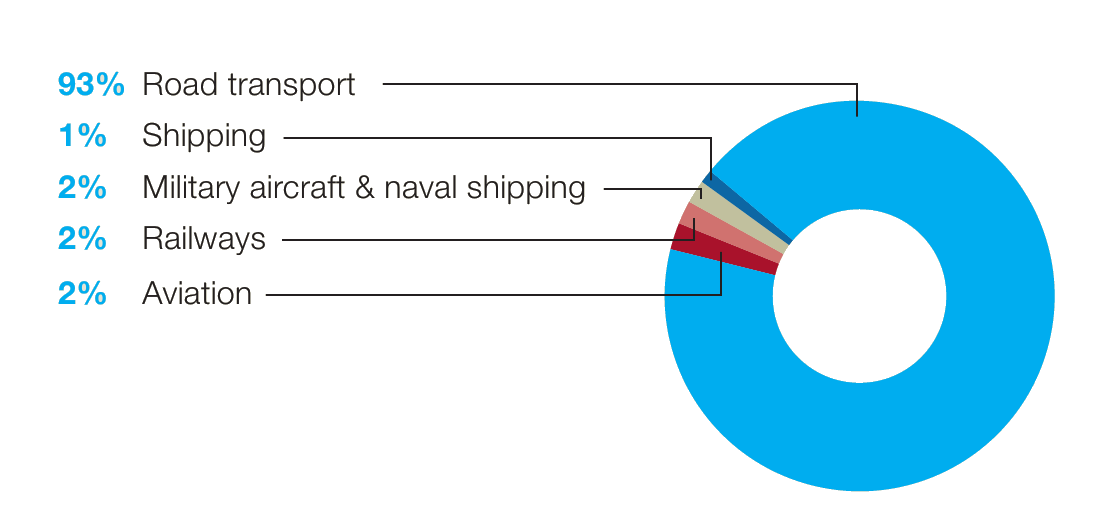
\includegraphics[width=14cm]{cc-trans.png}
 % cc-trans.png: 1113x529 pixel, 72dpi, 39.26x18.66 cm, bb=0 0 1113 529
 \caption{UK transport emissions by source in 2009 \citep{Decc2011t}.}
 \label{fig:cc-trans}
\end{figure}

An interesting feature of the UK's emissions reporting strategy is that
`transport' is generally presented as a monolithic category (e.g.
\citealp{Decc2010}), despite the wide variety of transport modes and purposes
presented in \cref{fig:cc-trans}. This makes it difficult to identify the
specific drivers of growth in UK transport emissions since 1970
\citep{Gasparatos2009} and stagnation since 1990 .
What is clear in
both cases is that energy use and hence emissions from transport have increased
(since 1970) or stagnated (since 1990) while those of other sectors have
declined. Between 1990 and 2010, transport was the only sector other than
housing in which emissions increased; transport now accounts for just over 20\%
of UK emissions (\cref{table:mtco2}, below). This research project quantifies
the contribution of commuting to this total in terms of energy use, and provides evidence
about which strategies may be effective for reducing the emissions due to
transport to work.

The UK's climate change commitments are unambiguous, agreed upon by all major
parties, and legally binding: emissions in 2050 must be below 20\% of their 1990
level \citep{ClimateChangeAct2008}. This means that the \emph{total}
permitted emissions in 2050 across all sectors are roughly equal to the emissions from
just the \emph{transport sector} today. This fact underlines the scale of the
proposed changes: transport to work represents a small but important component
of this challenge that affects millions of working people every day.


\begin{table}[htbp]
\caption[Top 5 UK sectors in terms of greenhouse gas emissions, 1990-2010]{Top 5
UK sectors in terms of greenhouse gas emissions, 1990-2010
(MtCO$_{2}$e). Data from \citet{Decc2011ff}}
\centering{
\begin{tabular}{lrrrrr}

 & 1990 & 2000 & 2010 & \multicolumn{1}{l}{\% change} & \multicolumn{1}{l}{\%
emissions (2010)} \\ \hline
Energy Supply & 273.4 & 220.1 & 204.3 & -25.3 & 34.8 \\ \hline
Transport & 121.5 & 126.7 & 121.9 & 0.3 & 20.7 \\ \hline
Residential & 80.8 & 90.1 & 89.9 & 11.3 & 15.3 \\ \hline
Business & 113.2 & 111.3 & 89 & -21.4 & 15.1 \\ \hline
Agriculture & 63.1 & 58 & 50.7 & -19.7 & 8.6 \\ \hline
Other & 117.4 & 65.8 & 32 & -72.7 & 5.4 \\ \hline
Total & 769.4 & 672 & 587.8 & -23.6 & 100.0 \\ \hline
\end{tabular}
}
\label{table:mtco2}
\end{table}

\subsubsection*{Emissions from transport to work}
% Something about transport being a challenging sector for emissions cuts
% Something about freight vs personal transport energy use and emissions
Of the 20\% of UK emissions that arise from transport, only a small fraction
are due to transport to work. How small? No official breakdowns of emissions are
provided by reason for trips, but estimates can be made by
analysing the make-up of the transport sector. As shown in 
\cref{fig:cc-trans}, 5\% of transport emissions can be accounted for by military
vehicles, aviation and shipping: none of these are usually involved in transport to
work. Also, 31\% of road transport emissions arise from goods vehicles (HGVs and
LGVs); the remaining 69\% arise from road vehicles for personal transport --
buses, motorcycles and cars \citep{DECC2011a}. From these figures, it is
possible to estimate that ~80 MtCO$_{2}$e result from personal travel in the UK.
19.5\% of passenger kilometres travelled by all personal transport modes in the
UK are due to travel to work \citep{DfT2011-why}. Transport to work
can be estimated to cause $\sim$16 MtCO$_{2}$e of emissions or around 3\% of the
UK's total. (In \cref{stotalcomp} a more refined estimate of commuter energy
use is presented, based
on geographically disaggregated data: commuting was found to account for
4.1\% of total energy use and 14.4\% of transport energy use.)

It is important to undertake such `back of the
envelope' calculations at the outset of research into emissions reduction
strategies or sustainable energy to ensure that time is not wasted on negligible
issues such as phone chargers \citep{MacKay2009}. David MacKay, Chief Scientific
Advisor at the Department of Energy and Climate Change (DECC), puts this
argument in lay terms by proposing a rule for
energy-saving interventions: ``A gizmo may be discussed only if it could lead to
energy savings of at least 1\% ... because the public conversation about energy
surely deserves to be
focussed on bigger fish'' \citep{MacKay2009-energyplates}. Applying this
reasoning more broadly to areas of energy use, transport to work clearly
deserves attention according to
this rule, although emissions cuts in commuting will have to be matched in all
other sectors for targets to be met. However, there are reasons to believe that
making cuts in the transport sector generally, and in transport to work in
particular, will be especially difficult, and therefore worthy of dedicated
investigation. These include:
\begin{itemize}
\item The transport sector is overwhelmingly dependent on petrol and diesel:
motorised transport (which accounts for most trips and the vast majority of the
distance travelled, as shown in \cref{Chapter5}) is 95\% %really!!!
dependent on refined oil products \citep{Woodcock2007}. This is problematic
because there are no commercially viable, low emissions alternatives to crude
oil for liquid fuels. Biofuels are the only `renewable' option on the table,
but their potential contribution is low \citep{Patzek2006,Michel2012}, they
can conflict with
food production \citep{Pimentel2009}, and currently used crops may increase
greenhouse gas emissions due to land use change \citep{Fargione2008}.
\item Linked with the previous point, low carbon technology is far less
promising in the transport sector than in other large emitting sectors.
% In electricity generation and residential heat demand, for example the %dad'd
For electricity generation and residential heating the technologies
for renewable alternatives are becoming more commercially viable \citep{Chu2012}.
By contrast,
the penetration of electric, hydrogen, and biofuel-powered cars may be slow,
largely due to their high cost \citep{Proost2011,AdamVaughan2011}.
\item The current transport system is built around road (and to a lesser extent
rail) infrastructure that took many decades and large capital investments to
complete. The dependence of society on the car is deeply embedded, yet a
low-energy (and hence low emissions) transport system may require a shift away
from personal ownership of automobiles altogether
\citep{MacKay2009,Moriarty2010}, something that will take decades to accomplish.
\end{itemize}
These difficulties make de-carbonising transport systems problematic
compared with the other large energy users --- electricity and heat
production.\footnote{These can convert more easily to renewable
sources --- e.g.~via stationary wind turbines
and solar hot water panels --- than can transport systems.
This is because transport systems are inherently mobile,
therefore requiring a high energy density power source.
Fossil fuels are unrivalled in terms of their energy density ---
almost 100 times greater than the best non-agrofuel commercial alternative:
lithium ion batteries. %!!!reference
Hydrogen fuel cells have been proposed as a solution, but these are
still far from commercial viability, and have been 
precluded by DECC's Chief Scientific Advisor on the
grounds that they are highly inefficient \citep{MacKay2009}.}
Despite these issues, transport is rarely framed in terms of energy use and
greenhouse gas emissions (\cref{Chapter2}). In addition to
its impacts on climate change via direct and indirect greenhouse gas emissions,
commuting is also vulnerable to the effects of climate change,
as discussed in \cref{s:uncertainties}.

\subsubsection{Climate change and energy}
Most studies looking at the impact of one aspect of the economy on climate
change do so through the emissions that it produces.
These studies generally measure environmental impact in terms of kilograms of
carbon or  CO$_2$ equivalent caused by different modes of travel.
This seems logical if one is concerned about climate change:
it is the greenhouse gases that trap the heat \citep{Houghton1990}.
However, others have suggested
that the best way to tackle the problem is from an energy perspective:
``climate change is an energy problem'', as a group of 18 prominent US
academics put it \citep[p.~981]{Hoffert2002}. What is meant by this is that
energy use and greenhouse gas emissions are currently two sides of the same
coin. More than 80\% of commercial total primary energy supply (TPES)
worldwide is provided by fossil fuels \citep{Smil2008} and in the
transport sector this is even higher.
It is true that not all forms of energy have the same emissions. Yet,
as illustrated in \cref{fgco2}, CO$_2$ emissions per unit energy are
in fact surprisingly similar across a wide range of transport fuels.
In addition, even if it were possible to decarbonise electricity
production in the near-term, the fact remains that uptake of low-energy sources
will almost certainly be gradual \citep{smil2010energy}. Another issue is
that technologies that have low emissions per unit of energy use during the
usage phase of their lifecycle often have an energy intensive production
phase. Because much modern food production depends upon fossil fuel energy,
the energy approach can also help in the
assessment of wide-boundary energy impacts.
Some environmental impacts of transport such as noise, road-kill and
the need to frequently resurface roads pummelled by powerful vehicles are not
included in most emissions estimates. Energy use can to some degree
encapsulate these additional impacts.

 \begin{figure}[htbp]
  \centerline{
    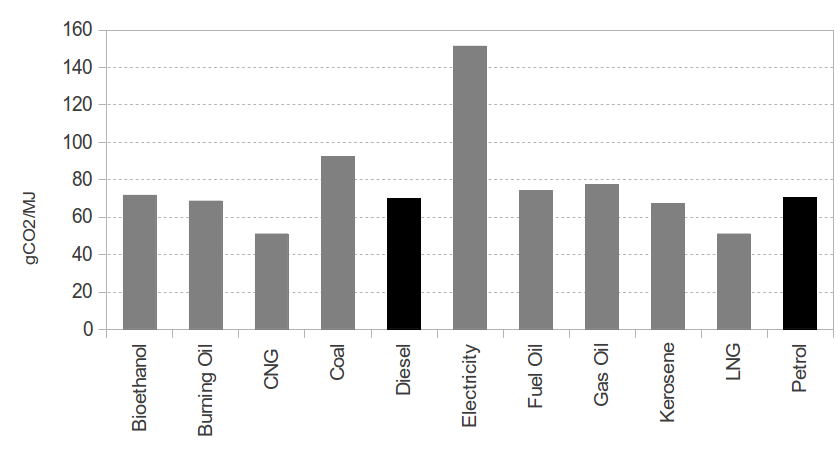
\includegraphics[width = 12 cm]{gco2}}
  \caption[The greenhouse gas emissions per unit energy of various fuels]
{The greenhouse gas emissions per unit energy of various fuels. Data
taken from \citet{Defra2011} (additional sources for
\href{http://www.ipcc.ch/pdf/special-reports/sroc/Tables/t0305.pdf}{\color{blue}electricity}
and
\href{http://www.biomassenergycentre.org.uk/portal/page?_pageid=75,163182&_dad=portal&_schema=PORTAL}{\color{blue}biofuel}
emissions were used)
and converted into SI units. The dominant
transport fuels are black for emphasis.  }
  \label{fgco2}
\end{figure}

The reasons for advocating a focus on energy use,
and not emissions directly, can be summarised as follows:
\begin{itemize}
 \item Emissions can be variable depending on the energy/fuel source, whereas
 energy is constant across fuel sources.
 \item If energy use is reduced overall, carbon-intensive forms can be phased out.
However, if emissions from one sector fall, they may well rise in another as
fossil energy resources are freed-up.\footnote{For
example, imagine if transport emissions rapidly dropped to zero
due to electrification and rapid uptake of renewables. The additional
load on the grid caused by this new user \citep{dyke2010impact} could
lead to an increase in the emissions stemming from space heating because
the total supply of renewable energy is fundamentally
limited by the laws of physics \citep{MacKay2009}. \citet{Berners-Lee2013}
describe this problem with emission reduction plans overall as squeezing
a balloon: savings in one area tend to bulge out in another.}
 \item Energy is the `master resource' from which all others (including more
energy) can be obtained; emissions are the end result of energy use.
 \item It can be argued that energy use is at the root of the linked `big picture'
problems mentioned in this chapter, not just climate change. Therefore
tackling the energy problem could have numerous co-benefits.
\end{itemize}
All this suggests that the climate debate should be much more closely
linked to the energy debate. Specifically, the carbon content of proven
fuel reserves should be compared with the carbon dioxide content that
can safely be burned. Doing this analysis, based on recently released
data on fossil fuel assets, has led to an alarming finding: ``for all the
talk about finite resources and peak oil, scarcity is resoundingly not the
problem. From the climate's perspective, there is far too much fossil fuel''
\citep[p.~29]{Berners-Lee2013}.
% In fact, to keep the chances of a
% global temperature increase below two degrees centigrade
% (the point beyond which many studies show would be dangerous),
% above 75\%, \citet{Berners-Lee2013} showed that humanity can burn only
% around a half of economically viable reserves.
\citet{Berners-Lee2013} show that for there to be at least a 75\% chance
that the global temperature increase remains below two degrees humanity can
burn only around a half of economically viable reserves.
In terms of personal transport, this means
phasing out petrol and diesel and avoiding carbon-intensive electricity sources:
a fundamental shift.

Most greenhouse gas emissions stem from fossil fuel use, and once
extracted, these fuels are invariably burned. This has led to the conclusion
amongst some that the solution must be top-down:
fossil fuel companies must be forced to leave most of their assets untapped.
This can be achieved 
either through plummeting prices of fossil fuels or through regulation.
The former case is currently highly unlikely due to the surge of fuel demand from
emerging economies, combined with the sheer utility of fossil
fuels.\footnote{However,
if governments, in coordination,
prioritise minimising energy use while maximising
uptake of renewable energy, the former possibility would become more feasible.
}
The latter also seems unlikely, following the failure of UN talks in
Copenhagen to arrive at a consensus on legally binding
and enforceable emission targets for the major emitter.
This research is relevant in any case: if fuel prices remain high there
is a strong economic incentive to reduce energy imports. If leaders worldwide
agree to tackle climate change through top-down or bottom-up
policies, there will clearly be a strong interest in how best to
reduce reliance on fossil fuels in every sector that is vital for
well-being. Regardless of the level of regulation (whether it
occurs at the point of extraction or use of fuel), it implies high consumer prices
for fuels, through policies such as taxes, a
`carbon cap' or even energy rationing.\footnote{Interestingly, high prices of fossil
fuels is also the end result of many scenarios of resource depletion, which
has historically been another major driver of research into energy and
transport \citep{Fels1973}.}
% At this stage, it is worth noting that some people,
% including a number of politicians, believe that
% anthropogenic climate change should not be a political priority. Climate
% contrarians, some funded by the fossil fuel industry itself,
% have managed to confuse large sections of the public.
Another pragmatic benefit of the energy approach is that even if one questions
the need to tackle climate change, the arguments to reduce dependence on
finite fossil fuels for other reasons are very strong.

\subsection{Peak oil and resource depletion}
In addition to the impacts of climate change,
depletion of our fossil energy resources is another non-negotiable
reason for transition away from fossil fuels, to a ``post-carbon'' economy
\citep{Heinberg2005, Heinberg2009, Heinberg2010, Kunstler2006}.
Oil is the most rapidly depleting resource yet motorised
transport is almost entirely dependent on liquid fossil fuels
derived from it \citep{Gilbert2008}.
Multinational personal transport industries tend to downplay or deny the risks
of peak oil, pointing to non-conventional oil resources and technological
advance as reasons not to worry. Prototype biofuels, electric cars and hydrogen
fuel cells are often cited as ways of overcoming high prices. This is ironic
because each technology is highly dependent on oil for resource extraction,
manufacture, distribution and waste disposal stages of their life-cycle: high
oil prices could make the batteries for electric cars, to take one example, even more
expensive, far out of the reach of the median global citizen.
%!!! income?
Each technology is still in the research phase of development,
relies on scarce public subsidies to be commercially viable and cannot operate
on the scale needed within modern transport infrastructures even if production
lines producing them were scaled up before a major oil shock. Biofuels, to take
the most heavily subsidised example, can only ever produce a small fraction of
current transport energy demand even if all available resources were exploited
to the maximum (\cref{f:biofools}).

 \begin{figure}[htbp]
  \centerline{
    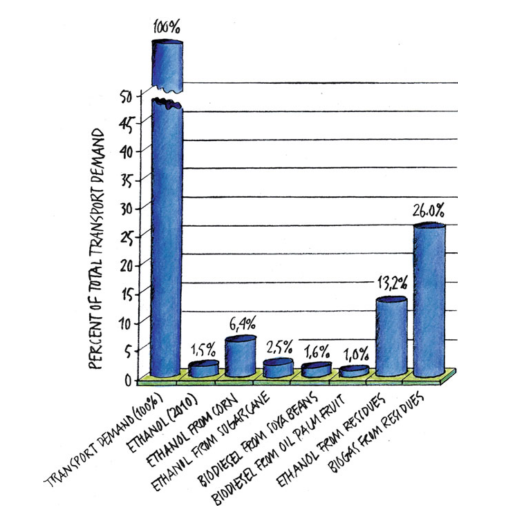
\includegraphics[width = 12 cm]{biofuels-cont}}
  \caption[Biofuels' contribution to global transportation energy use]
{Biofuels' current (2010) and potential contribution to
global transportation energy use \citep[p.~228]{Aleklett2012-peeking}.
Image used with permission of author. Data originally presented in
\citet{Johansson2010-ag-fuel+food}.}
  \label{f:biofools}
\end{figure}


For this reason peak oil is a major motivation for research into energy and
transport. How will transport systems operate beyond 2050,
when oil production will be a fraction of its current level? 
\citep{Aftabuzzaman2011}.
How will people get to work in the event of shortages?
\citep{Noland2006}. These are just a couple of examples of
the kinds of questions that are being asked in preparation for
declining oil supply. A parallel question
(explored in \cref{svul}) is: how will commuters be affected by
oil price shocks, depending on where they live and their socio-demographic
characteristics? The potential problems posed
by peak oil for motorised transport systems are severe and include
collapse of complex economic activity due to the
highly inter-dependent nature of the global economy \citep{Friedrichs2010,
Korowicz2011}.
For this reason an introduction to peak oil, and how it relates
to commuting, will help to place this research in the wider
context. \citet{Gilbert2008} provide a comprehensive reference
on the subject, from a North American perspective.

Peak oil is the point at which global oil production
enters terminal decline due to depletion of large oil fields
\citep{Greer2008}. It is an inevitable event during the 21$^{st}$
century, as oil is a finite resource, approximately half of which
has been used \citep{Aleklett2010}. However, there remains controversy
about the exact timing of the peak \citep{Smil2008}.
An in-depth review by the UK's Energy Research Centre \citep{UKERC2009}
found that the weight of evidence suggests a peak in the near-term,
before 2030. This is
well before the 20 years that the famous Hirsh Report \citep{Hirsch2005}
indicated would be needed to prepare for declining supplies of liquid fuel.
The implications are stark: if peak oil does occur before 2030, as
the evidence reviewed by \citet{UKERC2009} suggests, urgent preparations
must begin now.

As economists have long indicated \citep{Solow1974},
it is not only the amount of oil left in the ground
that directly affects peoples' lives. It is the \emph{price} of oil that
affects transport systems, with knock-on impacts on human lives.
Price is also affected by changes in demand and technologies for
extraction and substitution \citep{Perman2003}.
Over the past decade there has been increasing evidence that depletion
plays a major role in determining global oil prices, however,
with high and volatile prices likely in the future \citep{Aleklett2012-peeking}.
The price of crude oil during the past 20 years has shown both volatility
and (when a smoothed by a rolling average function) a near inexorable
upward trend \cref{fig:oilprice}. 


 \begin{figure}[htbp]
  \centerline{
    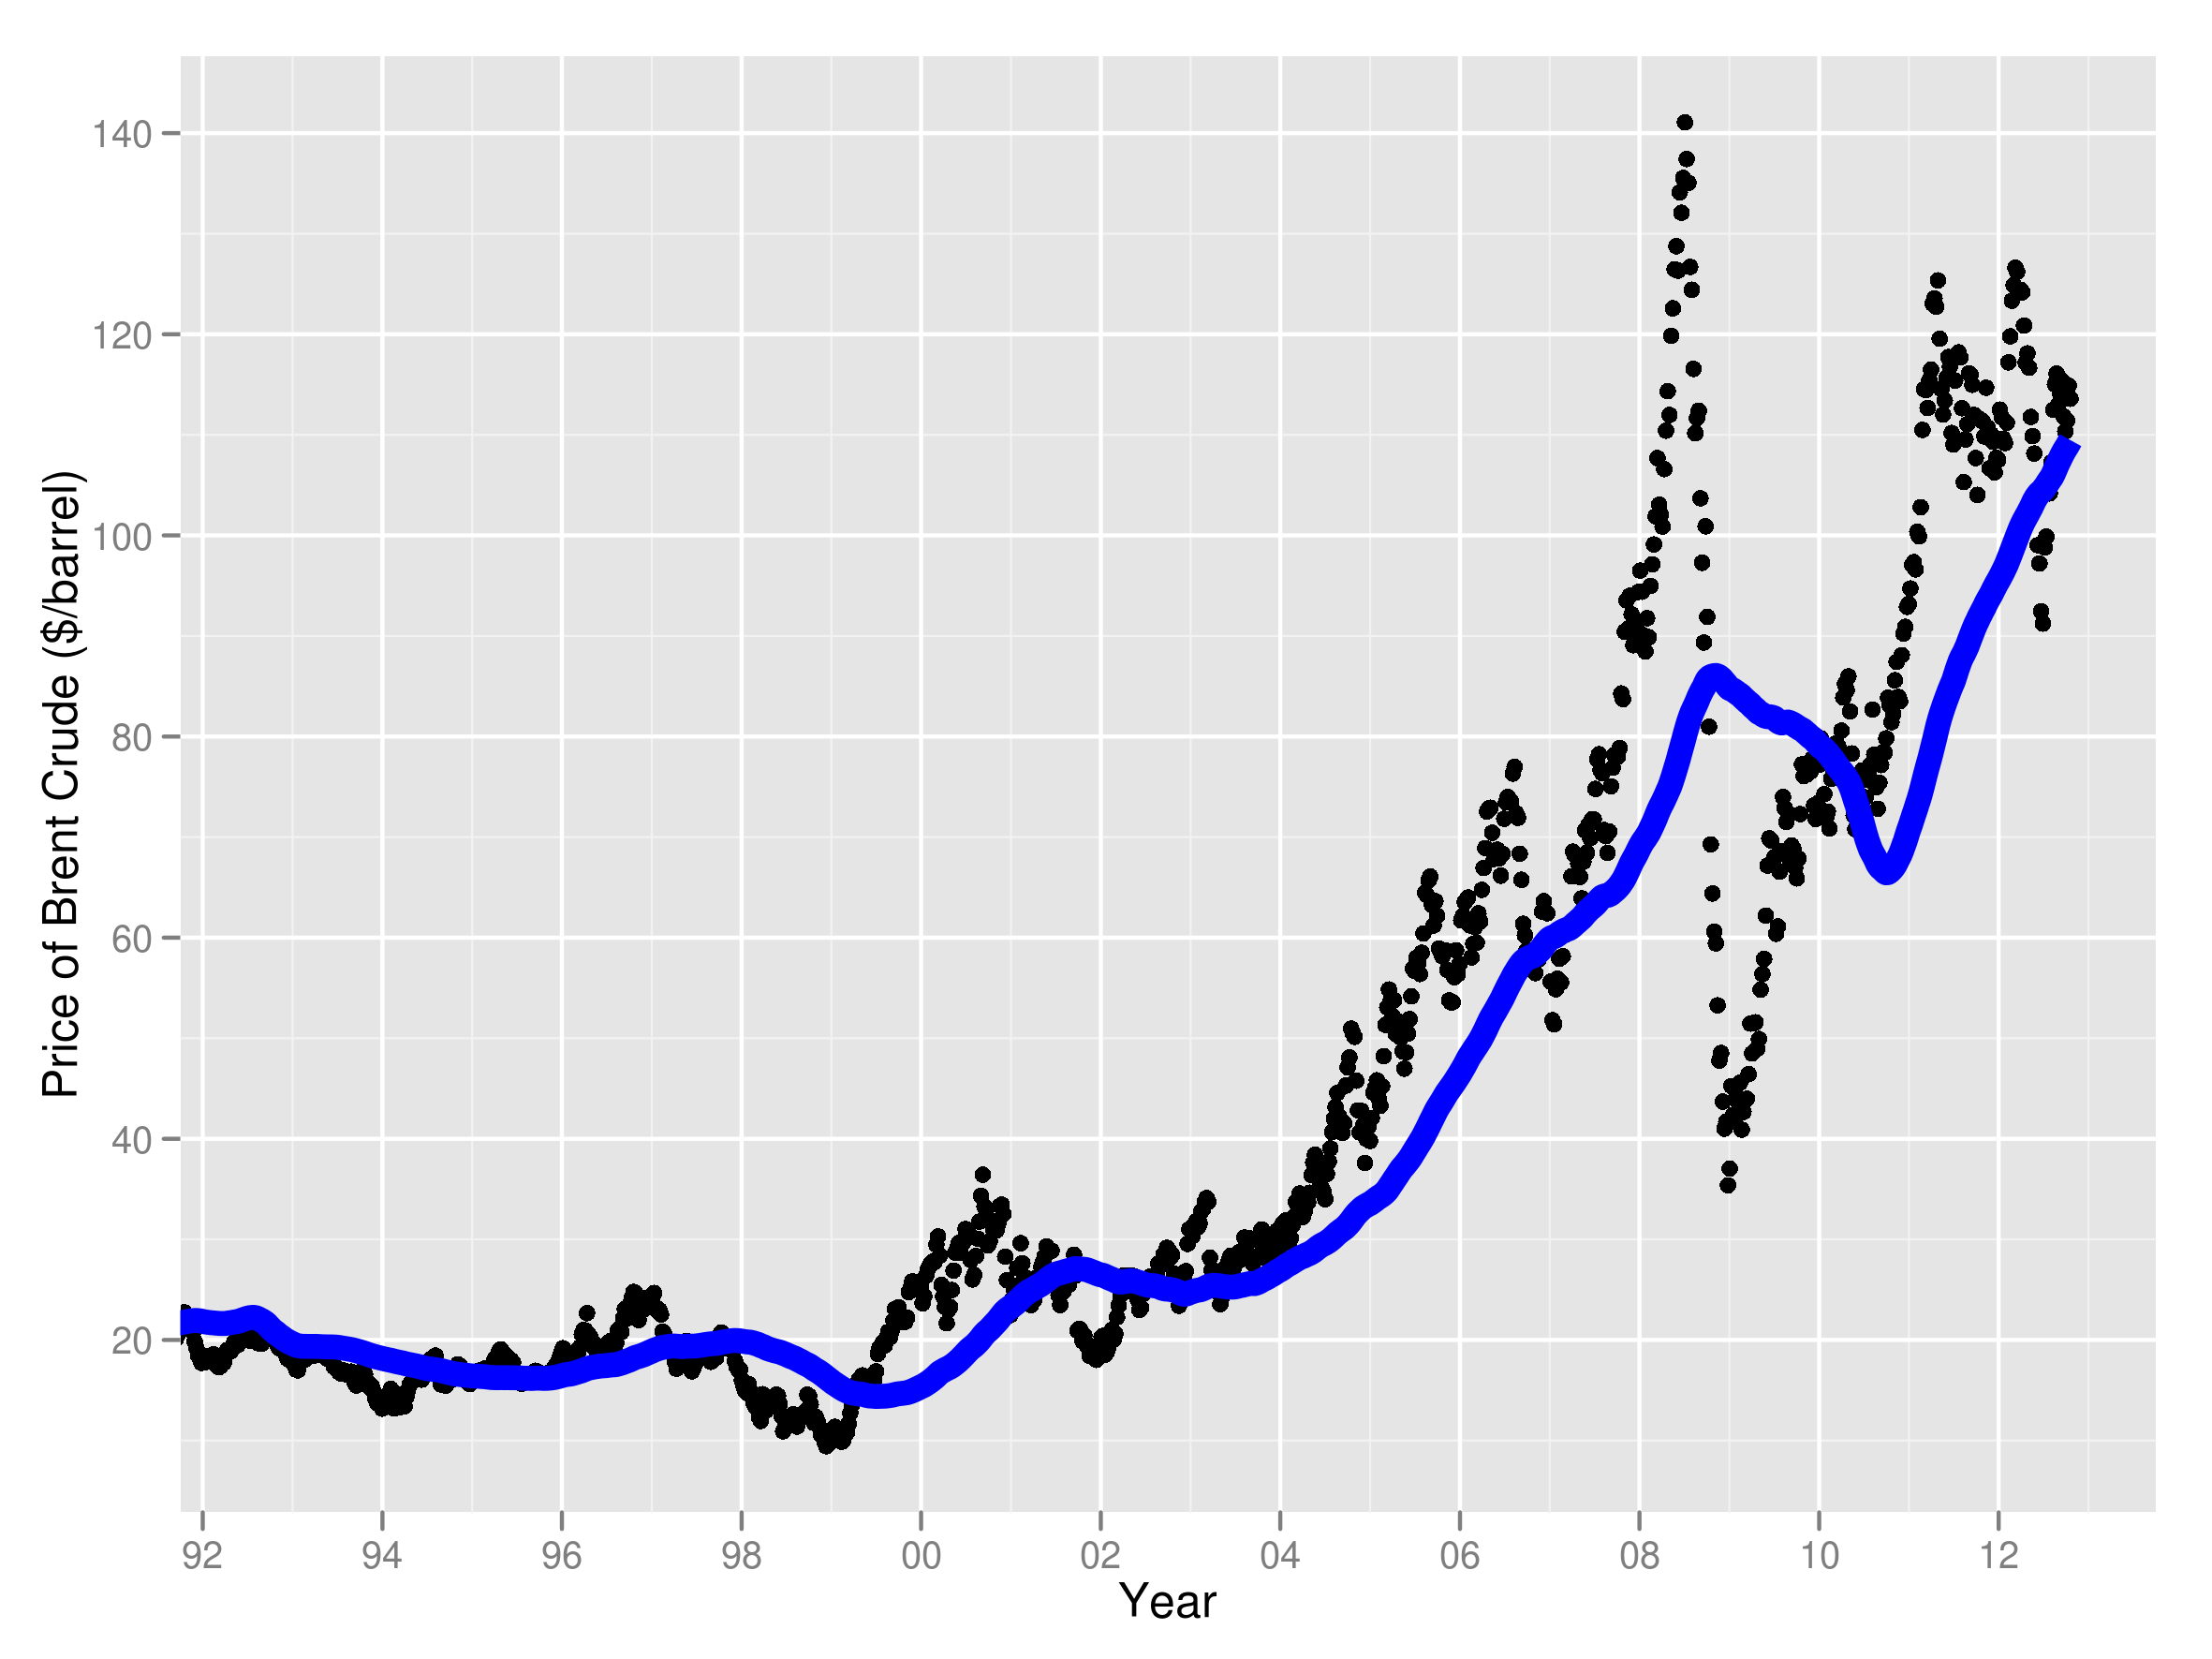
\includegraphics[width = 12 cm]{oilprices}}
    \rule{35em}{0.5pt}
  \caption[Average prices of Brent Crude oil spot prices, 1992 -- 2012]
  {Average prices of Brent Crude oil spot prices per week,
January 1992 until October 2012 (dots) and a 2 year rolling average
(blue line) Data from the U.S.~Energy
Administration (\url{http://www.eia.gov/dnav/pet/pet_pri_spt_s1_d.htm})
plotted using the R package ggplot2.}
  \label{fig:oilprice}
\end{figure}

Despite these upward trends, UK government energy policies
are still largely based on the assumption that oil prices will
remain below \$100 per barrel into the 2020s \citep{UKERC2010}.
Thus methods that estimate the oil-reliance of households based
on readily available commuter statistics could be highly relevant
to politicians and planners making long-term decisions. The ability to
quantitatively explore
the impact of high oil prices and other scenarios of change
at the individual level is an output of this
research that could have applications in transport policy evaluation and 
development. See \cref{Chapter7}.

\subsection{Inequality and well-being}
Peak oil and climate change are important because we
depend on the resources and processes of the natural environment to survive.
Humans also depend on the relationships between each other, not simply for
survival, but for quality of life. ``It is only in the backward countries of
the world'', wrote John Stuart Mill, ``that increased production is an
important object; in those most advanced, what is needed is a better
distribution'' (Mill 1857, in \citealt{Perman2003}: p. 6).

With more than 150 years of hindsight, Mill's statement seems all but
Utopian: economic growth is still the number one priority of most governments
worldwide, even in wealthy countries such as the UK where evidence
suggests that further growth may do more harm than good, for people and
the environment \citep{Latouche2008}.
To such an extent does economic growth dominate modern decision making,
regardless of consideration of how growth is distributed,
that authors such as Charles Eisenstein and John Michael Greer
refer to it as the founding story of our age \citep{Eisenstein2011, Greer2009}.
In contrast to this dogmatic growth focus, evidence suggests that
other things, including equality of economic and social opportunities, lead
to quality of life \citep{Jackson2008, Jackson2009}.

The growth-at-all-costs mentality, combined with our debt-based
capitalist economy\footnote{As explained by \citet{Eisenstein2011},
the very existence of positive interest rates ensures that those who
have money tend to have more. According to this view, growing
levels of economic inequality is built into the monetary system,
and can only revert back to low levels with crises such as
wars or depressions, planned debt annulments or
(preferably for Eisenstein) negative interest rates.}
has caused inequalities to grow worldwide
\citep{OECD2011}. The UK has one of the highest levels of
inequality in Europe (\cref{fig:ineqs}).

\begin{figure}[htbp]
  \centerline{
    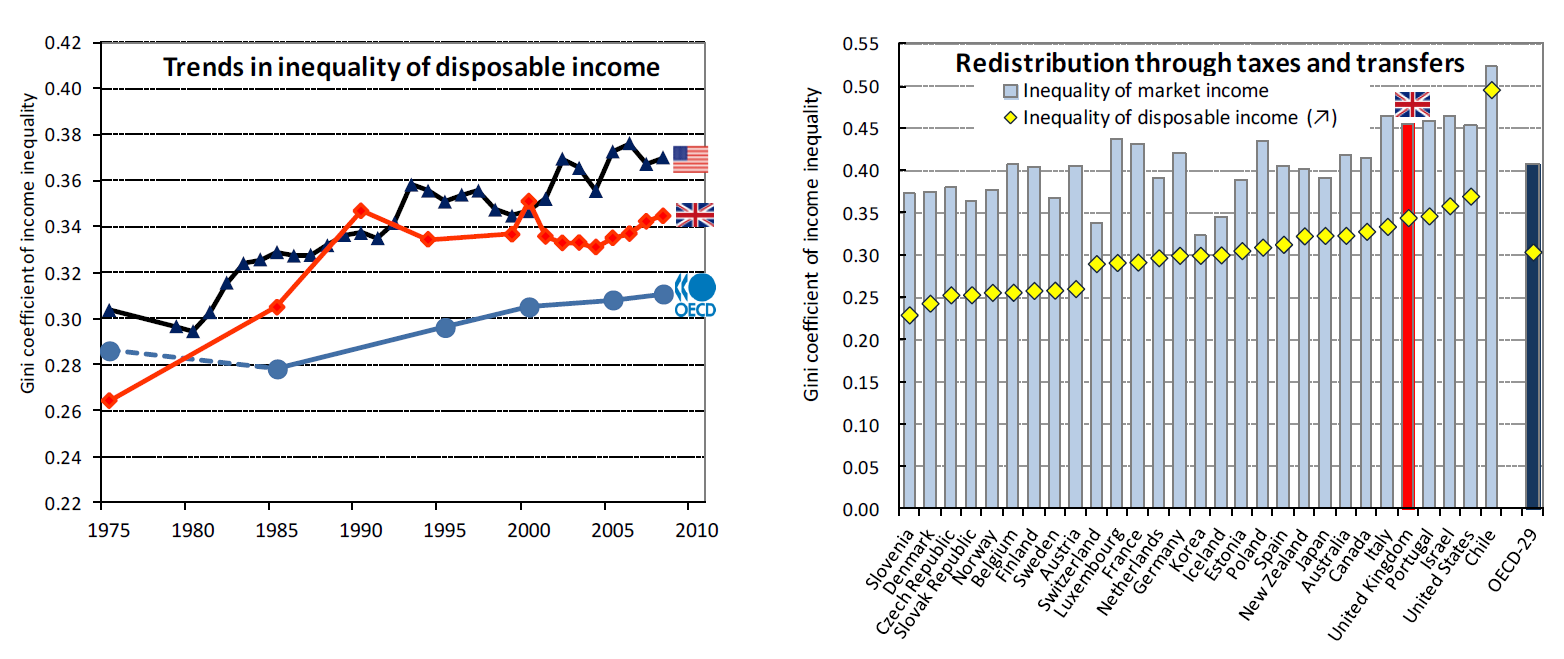
\includegraphics[width = 15 cm]{oecd}}
    \rule{35em}{0.5pt}
  \caption{UK Gini index for market and disposable income
  in context \citep{OECD2011}.}
  \label{fig:ineqs}
\end{figure}

This problem is important in the context of the energy costs
of commuting because employment opportunities are greatly
affected by one's ability to find and affordably travel to work.
Variable transport opportunities amplify social and economic
inequalities: 38\% of jobseekers say transport problems prevent
them from getting a job \citep{SocialExclusionUnit2002}⁠.  ``No jobs nearby'' and
``lack of personal transport'' were the first and second most
frequently cited barriers to getting or keeping a job in a survey
of young people in the UK \citep{Bryson2000a}⁠.

% \subsubsection*{Well-being}
% \label{s:well}
% In addition to the readily quantifiable impacts of commuting on climate change,
% rates of non-renewable resource depletion and (to a lesser extent) economic
% opportunities and inequality, the daily trip to work also has a direct impact
% on well-being. This body of literature can be divided into three main areas:
% commuting and physical health, psychological impacts and how the impacts
% of commuting vary between people, for example based on gender and class.
% Key papers in each of these areas are highlighted below.
% 
% Commuting involves a substantial amount of time, effort and expenditure. It
% is (for the xx\% of employed people in Britain who do not work at home)
% an essential component of daily economic life which.
% It is worth, at this stage, reflecting briefly on employment because if
% employment is an optional extra, the well-being impacts of commuting could
% simply be avoided by not working. However work appears to be integral
% to well-being for most adults.
Paid employment, and the
economic independence it brings, is a foundation for life satisfaction
\citep{Jahoda1982}. Work is ``a principal source of identity for most adults''
\citep{Tausig1999} and can promote good health (if the work is satisfying)
\citep{Graetz1993}. By corollary unemployment, the proportion of working-aged
people without a proper job, ``is a crucial indicator of the welfare and
economic performance of different areas'' \citep[141]{Coombes1982}. Yet without
accessible means of travelling to and from work each day, these benefits are
impossible to reach.

Given the importance of work, and the high proportion of work that is
undertaken outside the home, it should come as no surprise that
people will commute even if it an arduous task damaging to their health.
Taking a broad definition of health, these impacts range from those
narrowly associated with breathing urban air to more subjective consequences for
mental health including stress. From a human ecology perspective
commuting can be understood as a stressful relocation from one's
`domestic habitat' to a more hostile, hierarchical workplace. %%%%% ref!!!
The trip to get there will often coincide with thousands of other
commuters, all using the same road, railway or path. With these factors
in mind, the finding that, ``For most people,
commuting is a mental and physical burden'' should come as little surprise
\citep{Stutzer2007}.\footnote{The question
``how much of a burden'' is open to debate, however.
The finding of \citet{Stutzer2008}, that subjective well-being
declines proportionally with time, was not replicated in a
recent analysis of data from the BHPS \citep{Mumford2012}.}
The entrenched issue of inequality is tackled from
the perspective of commuting by measuring it in energy
(as opposed to purely monetary) terms (\cref{sindvar}) and providing
methods for assessing the distributional impacts of future
what-if scenarios (\cref{Chapter7} and \cref{Chapter8}).

% \subsection{Why energy?}
% The 

\section{Commuter energy use: everyday realities}
\label{s:realities}
The large scale processes of change mentioned above tend to be thought of in the
abstract, using inevitably simplified versions of reality. They are
often best represented through statistics, inherently simplified and
aggregated for visualisation. Seeing the issues quantitatively and
at `arms length' may be necessary to
gain an objective understanding of their evolution. Yet this may also lead to lack
of understanding of their local level manifestations and poor retention in memory:
although physical
reality may be best understood through numbers, human brains seem better able to
retain information that has emotional or personal content
\citep{Laird1982, Green2012}.
% \footnote{This enhanced recall for emotional information
% appears to be linked to emotional sensitivity in general
% which is generally higher for women:
% ``An individual’s level of emotional sensitivity
% was a stronger predictor of their emotional recall
% than their gender, suggesting that memory for
% emotional information is not determined by
% gender alone, but instead reflects a person’s
% sensitivity to emotional information in their
% environment. Thus, gender differences in memory
% for emotional information observed in the present
% study most likely reflect that women are, on
% average, more sensitive than men to the emotional
% aspects of their environment''
% \citep[p.~204]{Bloise2007}.
% }
When explaining my research to others, the following question
has been found to
effectively transform a purely academic and boring issue into something
interesting and relevant:
``What would a doubling of global oil prices mean for your family?''
For this reason, and to introduce some themes that
are used throughout this thesis in `layman's terms', this section is
based on a brief personal story: that of Chris Fisher.

Chris was born and bred in Weobley, a small town nestled between Hereford,
Leominster and Kington (\cref{fig:hereford}). Since finishing
at Weobley secondary school he has worked in a
wide range of jobs in the local area, including for Weobley's largest employer
(and sponsor of the village football team) Primasil and a local restaurant
called Joules. His current job, held for over 3 years now, is
to provide manual labour in Tyrrell's crisp factory.

\begin{figure}[htbp]
  \centerline{
    % 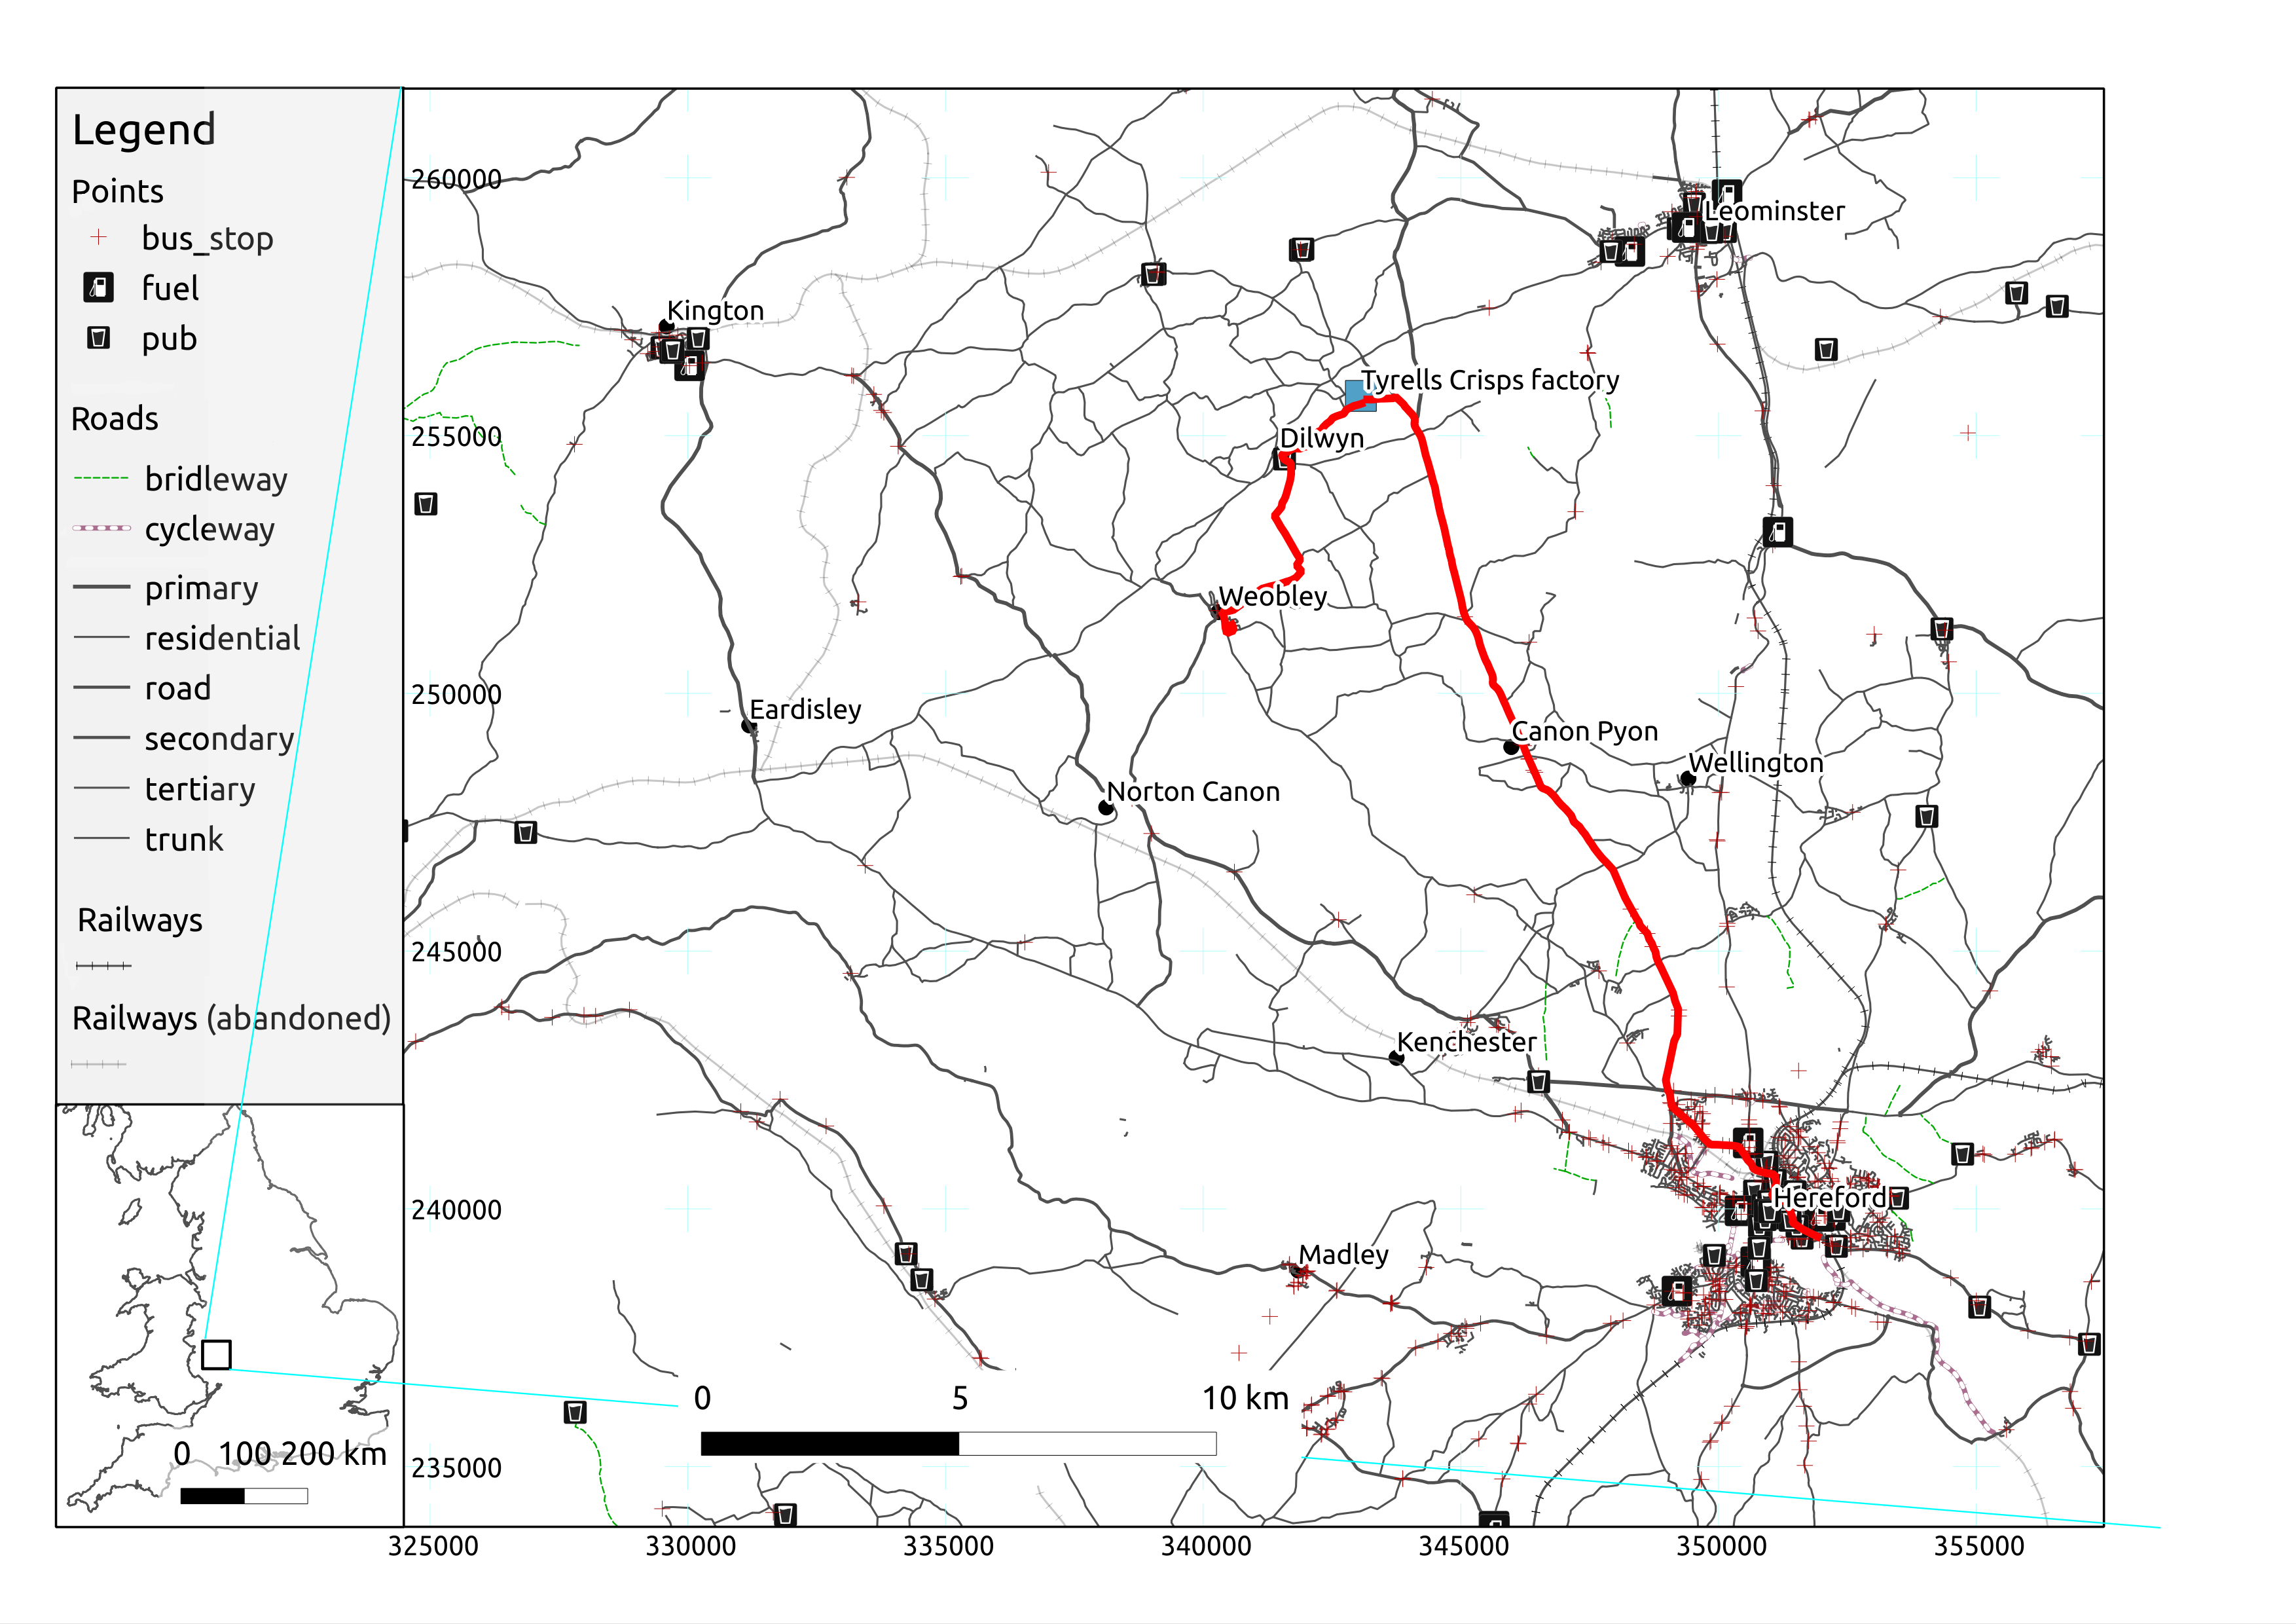
\includegraphics[width = 16 cm]{hnew}}
    \rule{35em}{0.5pt}
  \caption[Commuting options to Tyrrell's crisp factory]{Commuting options to
Tyrrell's crisp factory for Chris Fisher if he lives in Weobley (7 km one way)
or Hereford (13 km one way), as illustrated by the thick red lines.}
  \label{fig:hereford}
\end{figure}

Commuting and the economic cost it exacts has a large impact on Chris's life.
Ideally he would like to move to Hereford as that is where more of his
friends live and because there is more going on in the city than in Weobley.
However, Chris feels
bound to continue living with his mum in Weobley due to the costs of commuting.
The numbers work out like this: it's an 8 to 9 mile round trip to work from
Weobley, whereas the distance would approximately double if he lived in Hereford.
The location of his job also essentially forces car ownership: there are no buses
between Weobley and the Tyrrell's crisp factory, car sharing options are limited
and relying on a bicycle does not seem feasible for winter shifts that end at 6 am.
In addition to location, other downsides include long hours (12 hour shifts for
everyone, 4 days on, 4 days off), poor pay (\pounds8 per hour) and unpleasant
working conditions (the factory contains no windows, meaning that during
some day shifts you do not see the sun for 4 days in a row). For these reasons
Chris was tempted to quit when Tyrrell's decided to move towards 24 hour
production following increased demand from the USA: previous to this change
8 hour shifts were the norm; afterwards 12 hour shifts were implemented, broken up by
three 20 minute breaks.
% \footnote{This industrial regime is ironic given that
% part of Tyrrell's appeal is their `local' feel: on the company's website this is
% hammered home in the following blurb:
% 
% ``We're proud Herefordshirians [sic]
% (is that a word?), so we only use potatoes
% from local farmers, our favourites being Lady Rosetta and Lady Claire.
% They're the names of the potatoes, not the farmers.
% Just to be clear.''
% 
% In contrast to this artisan advertising, the management seem
% to treat the local employees as cheap labour rather than a treasured and
% unique group of people. For example, wage rises were promised following the
% implementation of 12 hour shifts but 6 months after the salary remains
% fixed at \pounds8 per hour, this time with no prospect of earning overtime.
% }


Despite these issues Chris has so far
decided to stay on at Tyrell's because
``if you live in Weobley, there are not many jobs.''
This context is important, because it illustrates how commuting
interacts with everyday life dilemmas, in this case
between moving house or staying put and
between quitting an exploitative job or finding a new one.
Ideally, Chris would like to sell his car, get a job in Hereford and be able
to walk to work each day. However, he's adapted to the new shifts, and
enjoys the 4 days of freedom he is allocated out of every 8, using them
to climb mountains, go to gigs and relax. The need to own a car
(on which 20\% of his income goes) and the expenditure on commuting
(5 to 10\% of his income) are disadvantages that can be endured for now.

Chris almost always drives to work. He has cycled a few times in nice weather
and would like to cycle to work more frequently. However, the
prospects for \emph{modal shift} are not great at present: his bike is not
much good, and the prospect of cycling 5-odd miles at 6 in the morning
after a physically punishing 12 hour shift is not attractive.
Chris is very interested in the cycle to work scheme, and believes he
would cycle more if he had a decent bike --- a friend was able to
get a \pounds900 bicycle through it. That's the semi-solution that
will be pursued in the short-term, and that goes well with Chris's
fitness hobbies.
When asked about the impact of the commute on his quality of life
Chris gave a short answer: ``not a lot really.'' For him commuting
is simply a means to an end --- to get to paid employment --- which
in itself is just a way to earn a living.

The sheer complexity of commuting on a national scale is well illustrated
by considering that Chris's commuting behaviour, plans and experiences
are just one data point out of hundreds of thousands. Subtleties of
his current behaviour,
% \footnote{For example he occasionally cycles and lived `car free'
% during 7 months last year.
% }
let alone the transient nature of his working
hours, shift patterns, home location and employment status are not
picked up by questions in the census or, to varying degrees, in the
national travel surveys (see \cref{Chapter4}). Nevertheless, the things that
Chris allocated importance to --- the distance to work, the time and money
costs of the commute and the availability of alternative modes --- indicate
that quantitative analysis of these aspects of the problem
of commuting is appropriate and relevant to everyday life.

There are certainly many unknown and highly varied individual circumstances,
such as Chris's that can never be squeezed into simple numerical models.
However, the variables about which good geographical data are available
(mode and distance) and the variables which can be calculated
with varying levels of uncertainty (e.g.~economic costs,
potential for modal shift), match the factors that held most
sway for Chris, except for the location of his friends.
% \footnote{Even this could in theory be estimated, based on central place theory.}

% \section{Commuting as a global phenomenon (dodgy)}
% Chris Fisher's experience illustrates the importance of distance,
% available modes of travel and economics in the humble journey to work for one
% individual. On the global scale, commuting is vast. It is a near ubiquitous
% indicator of a formal economy, and consumes huge
% amounts of time, resources, and money (fig. on country commuter distances
% would be mint here). A `back of the envelope' calculation suggests that ~ xxx TJ
% of primary energy are consumed worldwide during 2 billion daily commuter trips,
% excluding indirect energy costs such as vehicle production, fossil fuel
% extraction, and road maintenance.\footnote{
% %
% Add method here
% %
% }
%  To provide a sense of scale, this translates to 2\% of global primary energy
% use (xx EJ) and 4\% of oil consumption across the globe. Commuting is also
% complex, taking place in myriad contexts
% and by a plethora of different modes. Charcoal burners... ,
% Factory workers in ..., The challenges faced by Chris Fisher regarding his  8
% mile car trip to the Tyrrel's crisp factory in Herefordshire may not be
% representative of commuting worldwide, but its importance in everyday life and
% the problems it poses for welfare and sustainability found everywhere.
% 
% To reiterate, journeys to work are dynamic and
% diverse: their \emph{length}, \emph{mode}, and \emph{costs} vary depend on a
% range of range of factors that also change over time and space. These are the
% fundamental characteristics of commuting and the building blocks of this
% research. These three variables also determine another important characteristic
% of commuter trips: their energy costs. This abstract yet quantifiable variable,
% based in physical reality, is increasingly important in a world of emissions
% targets, environmental awareness, and depleting oil fields. A review of previous
% work on commuting indicates that its quantification is also often absent
% in transport and energy policy. For this reason the energy costs of transport to
% work is the main concern of this PhD: understanding its variability across
% space, time and between people and interpretting what these results may mean
% for future transport policies is the broad goal. Each section of this
% thesis contributes to this goal. Before describing the contribution of each
% chapter, it is important to understand a little about the case study region,
% and why it was chosen.
% 
% Could include section on Getting to work in a 'post carbon' future here.

\section{The importance of commuting} \label{snimportance}
The previous two sections have illustrated the importance of commuting
in terms of its impact at the individual level,
and in the global context. In many countries, however, the importance of
commuting can be investigated using a more detailed source of information:
national transport statistics. This section introduces
aggregate level travel to work statistics from the UK Census,
which form the foundation of analysis in the coming sections, and outlines
the variability of commuting patterns nationally.
Based on these statistics, it also illustrates the importance of
commuting in comparison with other reasons for travel.

% These statistics demonstrate that there is no single way to measure the relative
% importance of travel to work compared with other reasons for personal travel
% such as shopping and `the school run'.
% 
% The relative importance of commuting
% as a reason for trip will depend on how you value personal travel, whether number
% of trips, distance, time or energy use are considered as appropriate measures
% of ``importance'', or what constitutes `essential' travel.
% Do I mention each of these points?

% Overall, commuter flow data tends to be the most reliable
% source of personal travel statistics. This is because
% travel to work is regular and predictable in time and over space.
% Distance can also be estimated quickly, based only on matched
% home-work postcodes.

% These, and other defining characteristics of work travel such as
% rates of occupancy and  multi-purpose trips are also explored, towards the
% sections end. These national level data, placed in context, help to introduce
% commuting as a unique and important trip type and outline gaps in our knowledge.

\subsection{Trips}
Trips are the basic unit of travel, ``a one-way course of travel
with a single main purpose'' \citep[p.~6]{Dft2011-notes}. The data presented in
\cref{fig:trip-nums-gb} (and henceforth)
therefore counts the daily journey to work and
back as two trips. The value for commuting provided by this dataset
(150 trips per year) may therefore
seem surprisingly low, implying that people only work an average of 75 days per year
--- \citet{hall2011tourism} estimate that roughly
400 commuter two-way trips are made per capita
per year worldwide. However,
the National Travel Survey samples all citizens, including children and the
elderly; the average number of trips made by commuters --- the focus in this
thesis --- is estimated to be double this figure, around 320 (\cref{sfreq}).

\begin{figure}[htbp]
  \centerline{
    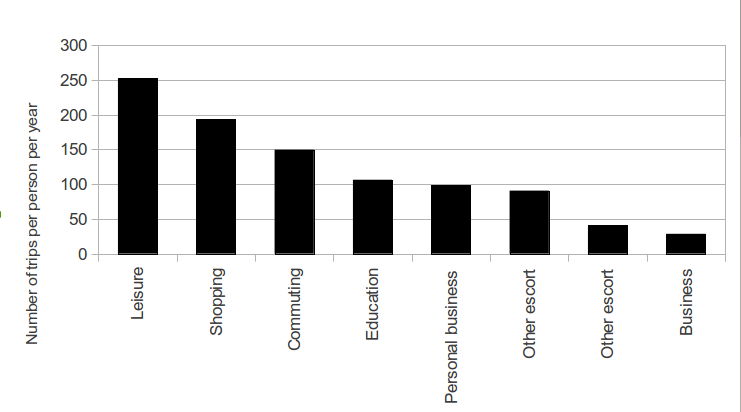
\includegraphics[width = 14 cm]{./Figures/trip-nums-gb}}
    \rule{35em}{0.5pt}
  \caption{Average number of trips per person per year across Great Britain.}
  \label{fig:trip-nums-gb}
\end{figure}

\subsection{Distance}
% The total distance of trips made by each trip type is equal to the number of
% trips made, multiplied by the average distance. Commuter trips averaged 14.2 km
% in 2009/10, slightly longer than the average trip distance for all trips Great
% Britain (11.3 km). Commuter trips are the third longest type of trips in the
% UK, following holiday and business trips, whose average values are greatly
% increased by flying. %Dad'd
The distance made by all trips is their number multiplied by their average distance.
Commuter trips averaged 14.2 km in 2009/10, slightly longer than the 11.3 km
average for all trips in Great Britain and the third longest,
following holiday and business trips. The average length of the latter
are greatly increased by flying.
This information
% , as well as the evolution over time,
are illustrated in \cref{fig:dist-trip-gb}.

\begin{figure}[htbp]
  \centerline{
    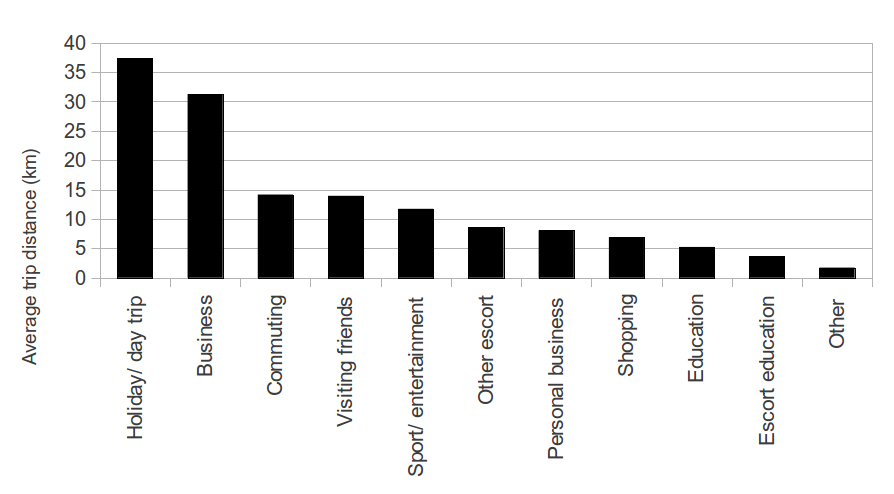
\includegraphics[width = 14 cm]{./Figures/dist-trip-gb}}
    \rule{35em}{0.5pt}
  \caption{Average trip length by purpose in Great Britain.}
  \label{fig:dist-trip-gb}
\end{figure}

The average distance of each trip helps characterise commuting as relatively
long-distance compared with other trip purposes such as shopping (6.9 km).
However, total travel distance is more important from an energy perspective:
long leisure trips, for example, are comparatively unimportant in energy terms if
they are infrequent. The data shows that leisure travel\footnote{Leisure
trips include holidays and social trips, in the 2010 National Travel
Survey \citep{Dft2011-notes}.} dominates trip distances, despite the sporadic
nature of international holidays. Commuting is in second place, responsible for
2160 km of personal travel each year for UK citizens, including those under 16.
For commuters, the average total distance of commute would be approximately
double this value (\cref{fig:dist-purp-gb}).

\begin{figure}[htbp]
  \centerline{
    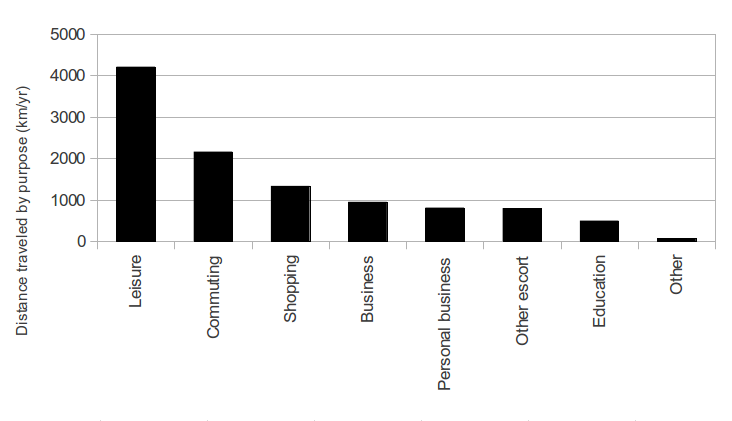
\includegraphics[width = 14 cm]{./Figures/dist-purp-gb}}
    \rule{35em}{0.5pt}
  \caption{Total distance travelled by mode in Great Britain.}
  \label{fig:dist-purp-gb}
\end{figure}

\subsection{Time}
\index{trip duration}
From the commuter's perspective, the number and distance of commuter trips made
may seem relatively unimportant: in the formal economy, time is money and
people are increasingly rushed to face up to professional and family
commitments \citep{Eisenstein2011}. Therefore, time is another measure of importance that
should receive attention in any introduction to commuting. Overall commuting is
the most time-consuming reason for personal travel in the UK, accounting
for 19\% of trip time, consuming 70 hours per year. Because both the numerator
and the denominator in this measure (hours per year) have time units, travel to
work can also be presented as the percentage of one's life spent travelling to
and from work\footnote{This
is a potentially poignant metric for those who
spend more than 5 hours per working day or more than 10\% of their life simply
getting to work and then turning around going home again!}
(\cref{fig:t-commuting}).

\begin{figure}[htbp]
  \centerline{
    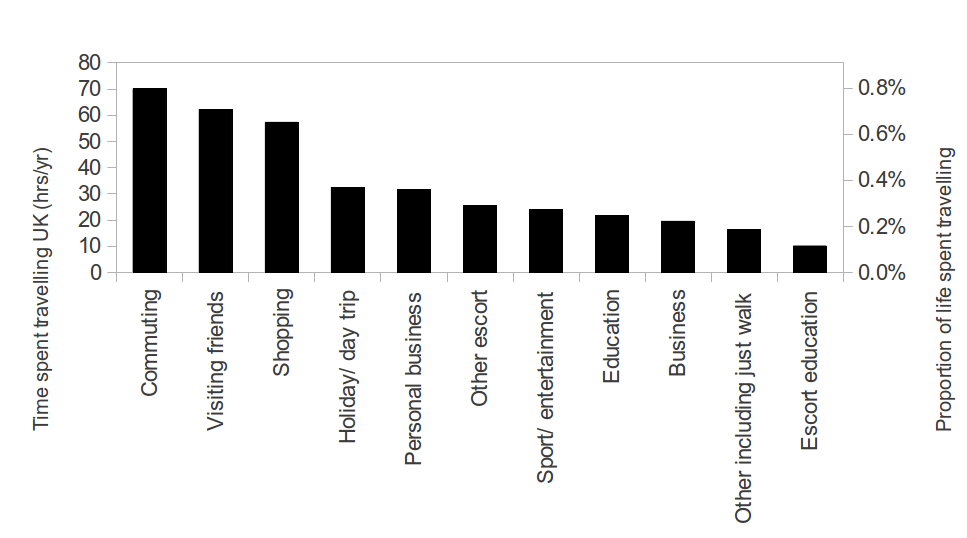
\includegraphics[width = 14 cm]{./Figures/time-commuting}}
    \rule{35em}{0.5pt}
  \caption[Time spent commuting in Great Britain]{The average time spent by
citizens of Great Britain travelling to work and back each year. The right hand
axis illustrates the same information, this time as a proportion (data
source: \citealp{NTS2012-time-travel}).}
  \label{fig:t-commuting}
\end{figure}

There is pronounced regional variation in the average time spent travelling to
work. This variation is linked to the average time per commuter trip (high
total work travel time values are influenced by how frequently people work),
the distance to workplace, and, of prime importance, levels of congestion.
% (\cref{fig:really?}).

% \subsection{Energy} % Include this!
% The energy costs of commuting is a complex subject with variability over
% time, space and from person-to-person. However, its relative importance
% compared with other sectors of the economy can be estimated rapidly,
% using simple `back of the envelope' calculations. 

% \subsection{How `essential'  is commuting?}
% The premise of this thesis is that commuting is essential for healthy
% functioning of modern civilisation, yet fundamentally unsustainable due
% to its use of energy. Certain trips for leisure and holidays are clearly
% discretionary, and could be discontinued with relatively minor
% consequences for the individual.
% Stopping travelling to work, in contrast, could result in unemployment ---
% with major impacts on well-being, as described in Section \ref{s:well}.
% However, one could equally argue that trips for shopping, the `school
% run' and to even to visit distant family members is essential for
% quality of life.
% Here, we consider different ways of classifying `essential trips' and
% the consequences for the importance of travel to work in the overall
% drive towards a sustainable national economy.
% 
% The simplest approach is to define commuting as essential and all other
% reasons for trips as superfluous. Based on this definition, travel to work,
% accounts for 100\% of essential trips in the UK. Under this (highly
% unrealistic) assumption, the best way to reduce the energy costs of
% personal transportation would be to reduce demand for other reasons for trips.
% Under this extreme scenario,
% children could be educated at home, food could be delivered by vans
% directed by internet transactions and communication with friends and family
% could occur online. Demand for trips to work, however ---
% seen as 100\% essential --- would remain unchanged.
% 
% Instead of this dichotomy (image of dichotomy!!!)
% 
% 
% 
% \section{The case study areas}


\section{Thesis overview}
The thesis is divided into 9 chapters which can be classified into four parts:
introduction, methods, results and conclusions.
Chapters 1, 2 and 3 provide background to the research. The present chapter
provides context. The purpose is to show how the thesis is motivated by
and informs some of the grand debates of the 21$^{st}$ century: environmental,
economic and social.
Chapter 2 is a more conventional academic literature review, focusing on the
research that is most closely related to the thesis topic rather than its wider
context. Chapter 2 tackles the following questions: what is the range of methods used
to investigate energy use in transport from a policy perspective? To what extent
is the literature coherent in its assessment of the reasons for energy intensive
transport behaviour and appropriate solutions? \Cref{Chapter3}
is the methodological literature review. It traces the various
incarnations and uses of spatial microsimulation and related methods.
The purpose is to illustrate
the reasons for choosing to apply the technique to the research questions
outlined in chapter 2.

Chapters 4 and 5 are methodological. The data available to analysts interested
in commuting are explained in detail in chapter 4, with reference to an ideal
dataset. Later in the same chapter, the underlying theory and computer code
developed and
used to generate spatial microdata is described in detail. The aim is to allow the
results to be replicated by anyone provided with the same input data as used in
the thesis. To this end numerous script files are provided which allow many
of the analyses performed to be re-run on any computer using free
software.\footnote{Sample code
and data used can be found here: {\color{blue}
\href{https://github.com/Robinlovelace/}
{github.com/Robinlovelace/}}
}
Chapter 5 describes and analyses the factors affecting energy use in personal
transport. Methods for converting CO$_2$ emissions data (the best official
source on the matter) into energy cost values per unit distance are described
and put to work on the best available data. \Cref{Chapter5}
culminates in a table summarising the best estimates for the
efficiency of each commonly used mode of travel to work.

The subsequent three chapters present the results and conclusions.
\Cref{Chapter6} harnesses the data and methods described in
previous chapters to
calculate the energy costs of travel to work at a range of levels, in England
and within the case study region of South Yorkshire. (A brief detour in
\cref{sinternational} compares English and Dutch commuter energy use
to illustrate the international applicability of the methods.) There is some discussion
of the links between energy use and other variables under investigation such as
home-work distance, mode of travel, age, sex and socio-economic class. However,
most of the results at this stage are descriptive: no
attempt is made here to evaluate political implications of the results. The
desirability of the commuting patterns that have been observed is more the
topic of \cref{Chapter7}, which discusses inequalities in commuter patterns.
% . The numbers are
% made to `speak for themselves' using a range of
% visualisation techniques.
In \cref{Chapter8} the attention is turned to the future. The analysis
is informed by `what if' scenarios made possible through spatial microsimulation
and a case study of `oil vulnerability' in Yorkshire and the
Humber.
The former creates quantitative scenarios to describe futures
of high cycling uptake and a shift to Finnish levels of telecommuting.
%!!! update this when c8 done!!!
Based on these assumptions, the total energy savings from each scenario is
estimated and the spatial and social distribution of the impacts
analysed. 
The latter investigates the likely impacts of high oil prices on
different social groups and places and is designed to show the policy-relevance
and usefulness of the methods.
% This links in with Chapter 7, which investigates
% inequalities in commuter energy use, and the related issue of oil
% vulnerability, in more general terms. These scenarios are
% based on evidence of reduced travel in a range of contexts, and how changing
% travel behaviours influence different sections of society.

Chapter 9 draws
together the various threads of the thesis to arrive at overall conclusions
about the energy costs of commuting: current patterns are not as simple
as first-impression thinking may indicate and neither are the solutions.
A particularly surprising result for the author was that cycling
can only make small savings in the current context compared with
the relatively overlooked options of telecommuting and car sharing.
% The methods allow
% other to check the results for themselves and tailor solutions to
% their specific situation.
% The aims and objectives that guide the thesis are as follows:

\section{Aims and objectives} \label{s:aims}
This chapter has argued that the energy costs of commuting is an
important and policy-relevant area of research, that links with
some of the major issues of the age.
This recognition of the potential applications of the research
is reflected in the aims and objectives. These, which have
helped to guide the research throughout, are as follows:

\subsection{Aims}
\begin{itemize}
 \item[A1] Investigate the energy cost of transport to work, its variability
at individual and geographic levels, drivers, and policy implications.
  \begin{itemize}
   \item[A1.1] Examine the variation of energy cost of trips to work, at
      geographic,	household and individual levels, and over time.
    \item[A1.2] Identify and explain the geographic and socio-economic factors
most closely  associated with high and low energy use.
    \item[A1.3] Formulate and analyse scenarios of change to inform decision
    makers about how commuter energy use can be reduced.
  \end{itemize}
  \item[A2] Explore and evaluate the potential of spatial microsimulation
models for the social and spatial analysis of the energy costs of commuting.
\end{itemize}

\subsection{Objectives}
\begin{itemize}
 \item[O1] Conduct a review of literature pertaining to the socio-economic and
geographical factors of
energy use and identify studies most relevant to the aims of this thesis.
  \item[O2]Calculate the energy costs of transport to work at different
geographic levels and interpret the results.
  \item[O3]Develop and use a spatial microsimulation model to simulate the
characteristics of different types of commuter and estimate the variability of
energy costs at the individual level.
  \item[O4] Identify the links between individual characteristics, geographic
variables and energy use
and analyse them further using the microsimulation model.
  \item[O5]Apply the energy use formula described by (Fels 1975) to individual
level commuting data to create estimates of the energy costs of transport to
work in Yorkshire (A1, O2).
  \item[O6] Formulate and test `what if' scenarios of future change in
variables
associated with commuter behaviour with the use of microsimulation and identify
the likely energy impacts of policy measures for commuters.
  \item[O7]Discuss the results in the context of high future energy prices and
the desire for reduced dependence on fossil fuels.
\end{itemize}

\subsection{Methods}
\begin{itemize}
 \item[M1] Descriptive statistics, time-series analysis, and GIS mapping (A1.1,
O2).
\item[M2]Development of a spatial microsimulation model (A1, A2, O3, O4).
\item[M3]Use the spatial microsimulation to investigate the impact of
change on commuter behaviour and energy consumption (A1.3, A2, O6, O7).
\end{itemize}







 % Introduction
%
% Chapter 2

\chapter{Personal transport, energy and commuting}
\label{Chapter2}
\lhead{Chapter 2. \emph{Personal transport, energy and commuting}}
% \lhead{Chapter 2. \emph{Commuting and its energy implications}} %
% \lhead{Chapter 2. \emph{The Energy Costs of Transport: A Review}}
\fancyhead[RO,LE]{Chapter 2. Personal transport, energy and commuting} %2side
\fancyhead[RE,LO]{\thepage}
%%% Really happy with this introductory text: reads nicely.
%%% Could I write this as a paper? May be worth it...

\begin{quote}
\textit{The traditional preoccupation with the supply side of transport policy
---
the provision of additional road, air and rail infrastructures --- is no longer
appropriate socially, economically and environmentally.}
\flushright{\citep[p.~5]{Peake1994}}
\end{quote}

Any review of research into the energy consumption of commuters is bound to
encounter wider issues such as transport infrastructure,
% --- which once in
% place, can affect transport flows for decades \citep{Whitelegg1987} ---
the spatial characteristics of labour markets \citep{Ballas2006}, population
densities of settlements \citep{Breheny1995}
and the price of oil \citep{Sexton2011}. Transport research is often
multidisciplinary \citep{Hoyle1992modern}. This element is even more important in
the present study because
commuting and energy use in transport are not academic disciplines, or even
established fields, of their own right. Rather they are issues, tackled from a
range of perspectives using various methods. 

As illustrated by the quote that opens this chapter,
research into energy in transport is
contested. Almost 20 years since it was written
there has undoubtedly been much more focus on the demand side;
social and environmental considerations have increasingly been
taken into account; and transport studies have become more
multi-disciplinary. Yet fundamental differences in the methods used by
researchers persist. Battle lines can be seen emerging in the literature,
for example, between those
who advocate a greater role for the social sciences \citep{Schwanen2011} and
those who advocate a scientific approach 
\citep{Simini2012, Marshall2008}. The transport-energy nexus has also received
attention from disciplines not traditionally associated with either issue,
such as computer science, physics and psychology.  It is therefore necessary to
impose some kind of order on the mass of work that is related to the topic.
With this aim in mind, the literature reviewed is divided into six sections:
\begin{itemize}
 \item the `sustainable mobility' paradigm (\cref{ssus})
 \item commuting research, at various scales   (\cref{s:commuting})
 \item energy use and emissions in personal transport generally (\cref{s:energy})
 \item energy impacts of commuting specifically (\cref{sdisciplines})
\item `tools of the trade' --- methods for studying energy and commuting
(\cref{s:tools})
\item key concepts in energy and commuting (\cref{skeyconcepts})
\end{itemize}
These sections initially deal with commuting and
transport energy use as separate entities,
because they have rarely overlapped. The studies that
do tackle the interface between these issues are generally conducted from
within pre-existing disciplines, such as economics or transport geography,
rather than adopting a completely multidisciplinary approach or attempting
to start a new field in `transport and energy', let alone
`energy use in commuting studies'.
\Cref{sdisciplines} therefore focuses on two studies
that deal with energy and commuting from two different perspectives:
transport geography and economics.
% have most to say in this
% regard, but drawing disciplinary boundaries in the field is probably
% not useful, so the section is structured by the research focus
% (life-cycle analysis, energy use of different modes etc.).
Because this
research area is quite specific, the section is the only one in which
comprehensive coverage is attempted. The other sections attempt
only to outline influential strands of research and highlight findings
of direct relevance to this project. \Cref{s:tools} provides
an overview of the techniques used in the research areas covered, and introduces
one of the main methods: spatial microsimulation.
(The spatial microsimulation literature is covered in more detail in
\cref{Chapter3}.)
The current chapter
concludes with a summary of important knowledge gaps in the area of
commuter energy costs, and promising research directions that
are related to the thesis (\cref{sc2sum}).
%%% This where we've hit the end (the section is only 1 paragraph long - Jan 2013)
%%% Ideally each section should be ~2,000 words long (10,000 / 4), less with images.

\section{The sustainable mobility paradigm} \label{ssus}
As outlined in \cref{Chapter1}, energy use in transport is bound up with a
number of issues --- climate change, energy, inequality.
Diverse as these are, they all fall within
the umbrella term of sustainability. It is not surprising, therefore, that much
of the work linking transport and energy use has been conducted within the context of
sustainability, especially since the 1990s when sustainability became a buzzword
in politics and academia. Here is not the place to discuss
of what sustainability does and does not mean.\footnote{See \citep{Pezzey1997} for an
attempt to define the term rigorously or \citep{Steg2005} for a discussion
of `sustainable transportation'.
}
For the purposes of this section, suffice to
say that sustainability relates to \emph{long-term} environmental, social and
economic well-being. According to \citet{Banister2008}, in a paper with the
same title as this section, sustainable mobility is an approach to transport
research and policy that differs from conventional transport planning priorities
in the following ways:
\begin{itemize}
 \item its focus on people and social outcomes rather than infrastructure,
 vehicles and traffic
 \item localised and specific in its approach to intervention, rather than large
 scale and homogeneous
 \item a focus on potential scenarios of the future rather than univariate `modelling'
 \item travel modes placed in a hierarchy with pedestrians and cyclists at the top,
 rather than a focus on motorised transport
 \item multi-criteria assessment methods used for project assessment
 rather than just economic valuation
\end{itemize}
On all counts, the world-view adopted in this research project
fits firmly into the sustainable mobility
paradigm, so this is the starting point for the literature review. Energy use
in personal transport may seem a technical consideration, suitable for consideration
only by traffic engineers and natural resource economists. Yet the energy intensity
of transport systems has a direct impact on resource depletion (and therefore
economic sustainability), the natural environment and, by amplifying inequalities
in access to physical and cultural resources, people's lives.
The energy costs of commuting are therefore of critical importance to
the ability of modern economies to sustain themselves.

Probably the most high-profile UK government report written from the perspective
of the sustainable mobility was published by the Sustainable Development
Commission (SDC) \citep{Kay2011}.\footnote{This report, incidentally, was
published just before the SDC was dissolved
by the coalition government in March 2011. No follow-up research
in the area has been conducted.
}
`Fairness in a Car
Dependent Society' takes
a broad perspective when analysing personal transport.
As advocated by \citet{Banister2008},
it focuses on people rather than traffic and infrastructure, while also mentioning
the potential for environmental and (long-term) economic gain.
The report urges the prioritisation of
``quality of life, safety and the environment'' for all members of society
affected by personal travel systems over the speed and convenience of
wealthy travellers \citep[p.~5]{Kay2011}. The report's findings are
especially powerful because it provided a very large body of evidence
to support its findings, rather than to simply repeat the `anti-car' mantra
expounded by some based on the strength of rhetoric, social theory and
a smattering of technical facts (e.g.~\citealp{Dennis2009}).
% An example of this insistence on evidence to support the argument
% is presented in \cref{fcrashnssec}: the simple visualisation
% vividly illustrates the problem in an politically neutral way, for
% maximum impact. Although traffic-related deaths and injuries are outside
% the scope of this PhD, the approach to quantitative evidence embodied in
% \cref{fcrashnssec} is something to which this thesis aspires.
% 
% \begin{figure}[htbp]
%   \centerline{
%     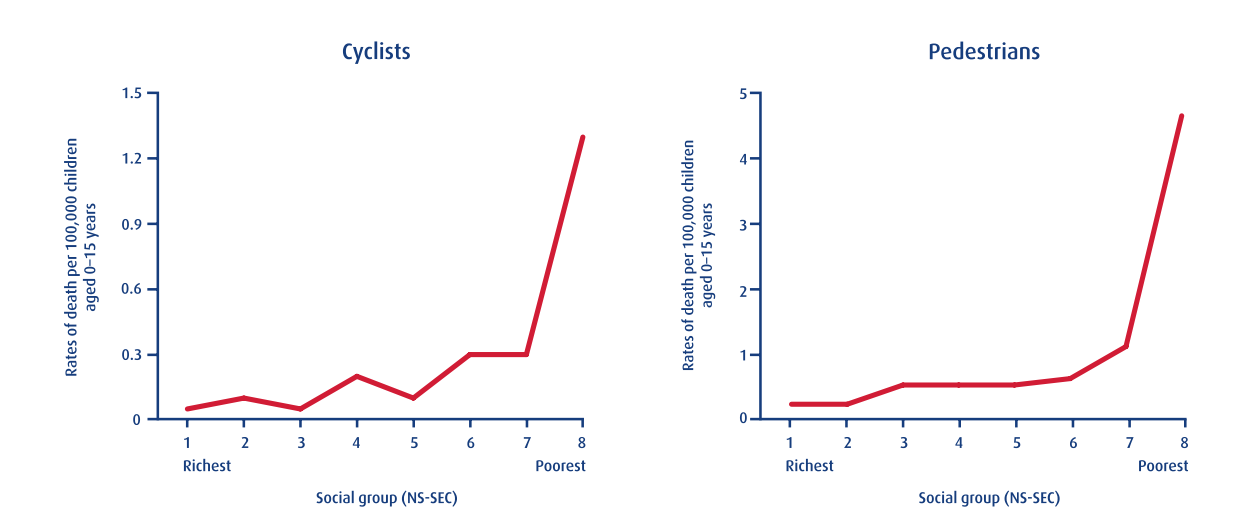
\includegraphics[width = 14 cm]{crashesnssec}}
%   \caption[The relationship between class and traffic-related deaths]
%   {The relationship between social class and traffic-related deaths
%   \citep{Kay2011}}
%   \label{fcrashnssec}
% \end{figure}

\citet{Kay2011} is also useful as a source of inspiration about
future interventions, as it provides %!!! mention kay in concs.
strong and specific policy recommendations. The most general of these, that 
can be applied to nearly every intervention affecting transport, is that a clear order
of priorities should be followed by transport policy-makers (\cref{fsdc}).
Incidentally, this is the same order of priorities that would be
followed if reducing energy use were the primary objective of
transport policy, as the evidence presented in chapter 1 suggests it should be.

This thesis is therefore closely related to the SDC study (and
the sustainable mobility paradigm more generally) in a number of ways.
It begins from the same world-view as \citet{Banister2008}, but
focuses on energy as a way to include all the various
factors affecting sustainability. The purpose of this research mirrors
that of \citet{Kay2011}:  to highlight the wider impacts of
personal mobility.
The methods are quite different, however: based \index{fairness}
on the knowledge that a range of social, economic and environmental ills are
associated with energy intensive transport highlighted in \cref{Chapter1}, the focus
is on
% not on the fairness and social outcomes favoured by \citet{Banister2008}
% and \citet{Kay2011}, but
energy use. This thesis does also
highlight the wider costs to society of personal travel advocated
in the `sustainable mobility paradigm', but indirectly,
via energy use, and with a focus on only one type of trip: commuting.

\begin{figure}[htbp]
  \centerline{
    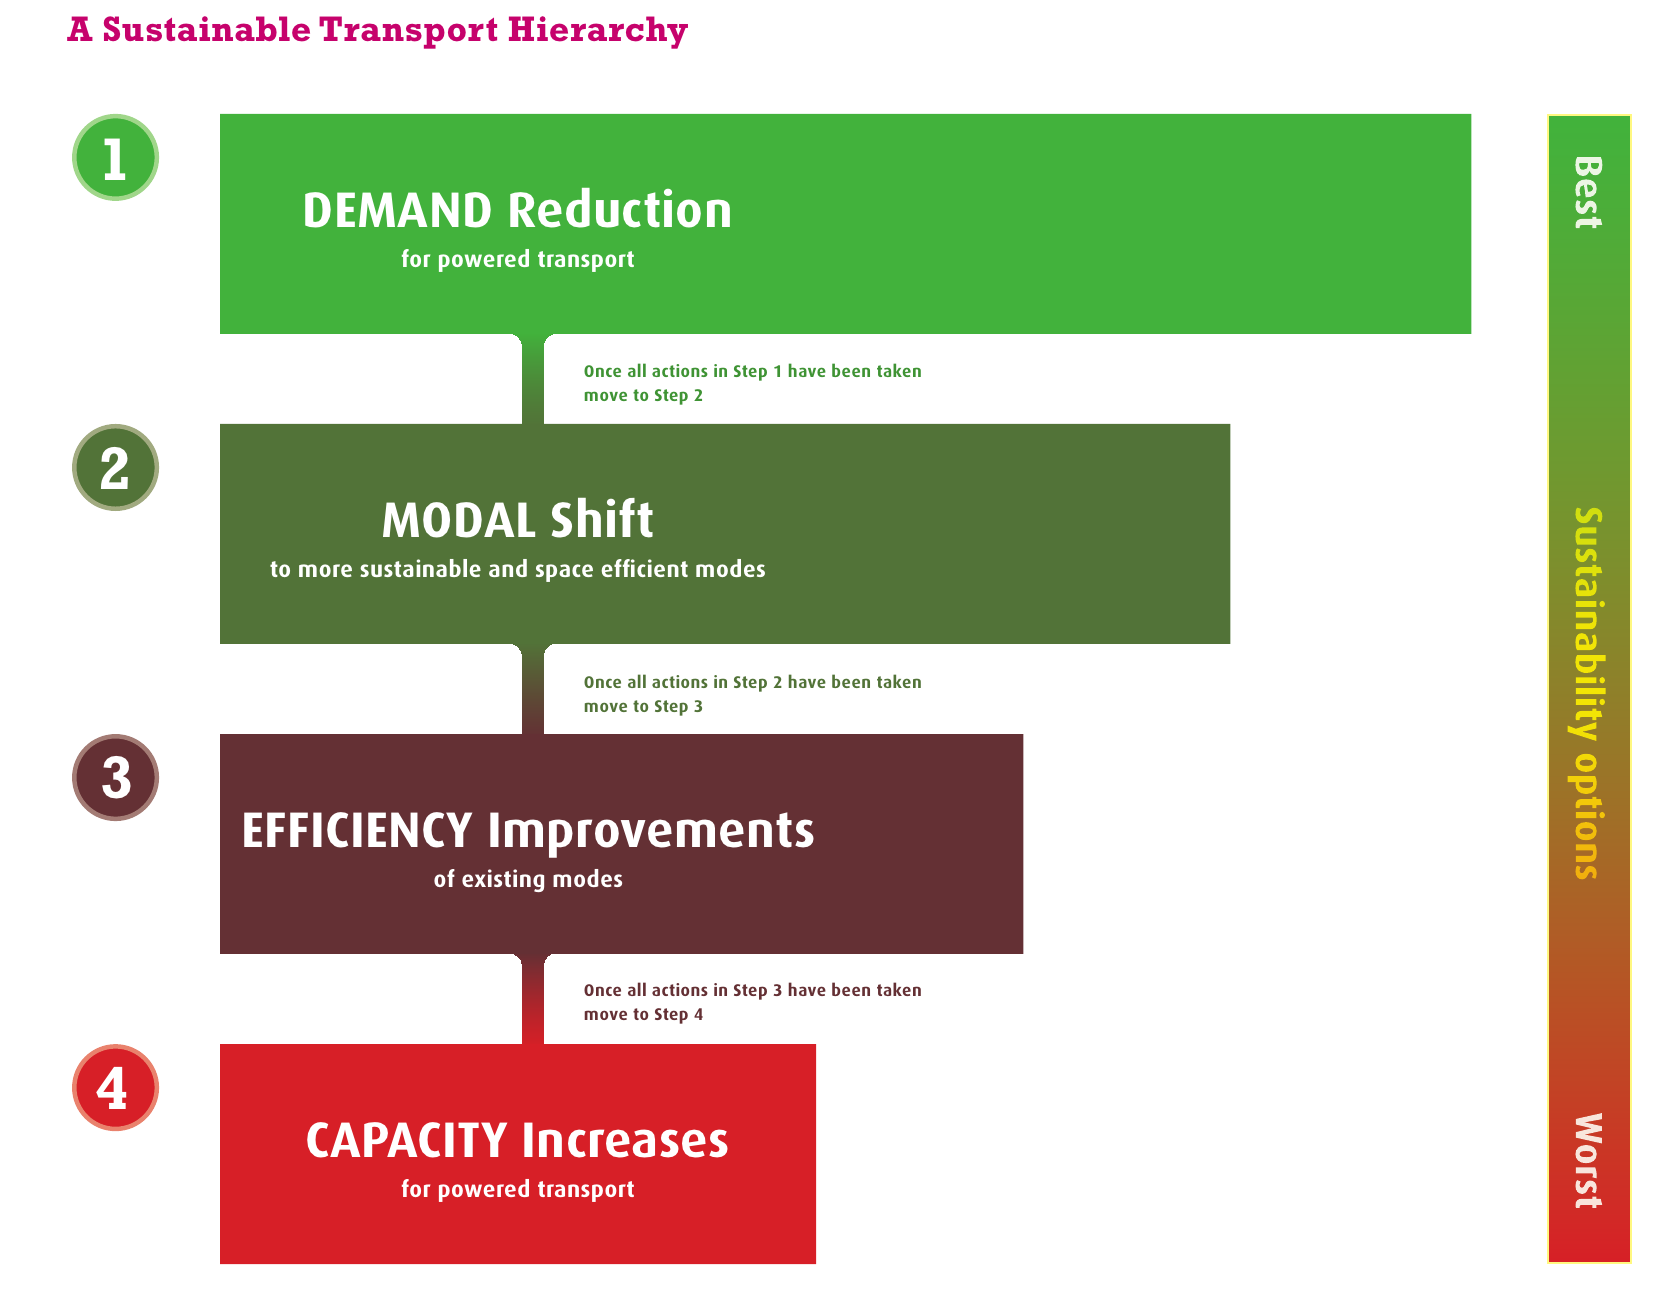
\includegraphics[width = 10 cm]{Sustainable-trans-hierarchy}}
  \caption{The sustainable transport hierarchy \citep{Kay2011}.} %%% could update with methods
  \label{fsdc}
\end{figure}

\subsection{Active travel} \label{sactive}
Although not always explicitly part of the sustainable mobility
paradigm, many of the studies from the loosely defined `active travel'
literature\footnote{This
area of
research has also been referred to `non-motorised transport', or simply
`walking and cycling'. The term `active travel' is preferred as it is more
concise and encapsulates all methods of travel to work that rely on human
muscles rather than mass-produced motors as prime-movers (see
\citealp{Smil2008} for more on the contrasts and surprising similarities between
the two). The rare but growing category of muscle-motor hybrid vehicles such as
electric bicycles is ambiguous is in this regard: as the ratio of motive energy
provided by personal exertion and inanimate energy sources will vary between
zero and infinity from case to case. The approach taken here is to exclude it
from active travel completely as motors and their energy supply must be
included for a realistic energy assessment.
%ref
}
make reference to the sustainability benefits of walking and cycling. For
the purposes of this literature review, research into non-motorised modes is
therefore considered as part of sustainable mobility,
although the term has been used in different
contexts.\footnote{Lawrence Burns, who directs the Program on Sustainable
Mobility at Columbia University's Earth Institute,
uses `sustainable mobility' primarily to describe shifts in
car technology and use, including driver-less cars and electrification \citet{Burns2013}.
\citet{Aftabuzzaman2011} uses the term to describe a transport system
resilient in the face of peak oil.
}
Much
of the active travel literature
has a clear health agenda (e.g.~\citealp{Jarrett2012}); here the focus is
on studies that also report energy and emissions implications.

\citet{Woodcock2007} investigated the links between transport, the environment
and health by projecting the rate of active travel up to 2030 in London.
The outcome of policies to encourage cycling were found to be wide ranging,
including positive impacts on road injury rates (a `neglected epidemic'), physical
inactivity and associated degenerative diseases, climate change and pollution,
`community severance', as well as difficult-to-measure impacts on energy
security and rates of transmission of infectious diseases. Clearly it is not
possible to accurately measure each of these impacts in a single study, but
it is useful to bear in mind the broader benefits of walking and cycling, which
are also particularly energy efficient. In a similar vein, \citet{Jacobsen2009}
provided evidence to suggest that as well as competing with healthier
and lower-energy active travel modes
for trips and space, motorised traffic also discourages walking and cycling
through perceived danger levels. Although their methodology was relatively
rudimentary (a review of statistics from the academic and policy literature),
\citet{Jacobsen2009} provide the basis for an interesting hypothesis:
that strategies to reduce
car use may be more effective than pro-active travel measures in terms of energy
and health outcomes. The case study comparing commuter energy use between
the UK and the Netherlands presented in \cref{sinternational} provides some
empirical support for this hypothesis.

With the emergence of newly available datasets from GPS devices, mobile phones
and bicycle rental schemes, more sophisticated methods have emerged in
the realm of active travel research. \citet{Ogil-cambridge2010}, for example,
provide details of how GPS measurements for individuals can be used
estimate both physical activity levels and CO$_2$ savings of active travel.
In-depth questionnaires were also used to estimate
``physical activity energy expenditure (PAEE) and total energy expenditure (TEE)''
\citep[p.~7]{Ogil-cambridge2010}. GPS data was combined with
accelerometer data by \citet{Cooper2010} to estimate physical activity. Although this
metabolic energy consumption of the human body is not
generally seen in the same light as energy use by vehicles, both can be measured
in the same units and compared directly. It is argued in \cref{Chapter5} that
this fact is a further benefit of the energy approach to commuting: substituting
motorised energy use with muscular energy has a direct impact on obesity and
chronic inactivity levels. Thus energy measurements can
encapsulate (to some degree) health as well as environmental impacts of travel.

In line with this new abundance of data, advances have been made in
characterising and 
modelling active travel patterns as well. \citet{Millward2013} used GPS
data to supplement survey findings on walking trip characteristics in a US
city. The combination allowed for accurate characterisation of both
quantitative variables such as speed, time and distance of travel as well
as qualitative information about the reason for the trip.
Of particular relevance to scenarios of
future change, is work looking at the `impedance functions' of active travel
modes with respect to distance under various conditions \citep{Iacono2010}.
Here, impedance refers to the disincentive to make trips by active travel per
unit distance.
Impedance influences $p$, the proportion trips that
take place between A and B made by walking or cycling. Due to the impedance or 
`resistance' to travel associated with these modes being highly dependent on distance
compared with faster and 
less physically demanding motorised modes, the proportion of trips made by them
can be expressed as a function of distance ($p = f(d)$). Based on this reasoning
$p$ should be high for the shortest
trips, dropping rapidly as the distance increases beyond a few kilometres
and levelling-off towards 0\%  after around 5 km for walking and 15 km for cycling. 
This hypothesis has indeed been born-out in practice.
Based on travel survey data, \citet{Iacono2010} calculated the rate
at which the proportion of trips made by bicycle and walking decreases
with increasing distance for different trip reasons, including shopping and
commuting \cref{fimpedance}.
The average proportion of trips ($p$) made by a particular mode in a particular context
(e.g.~bicycles for shopping in a given settlement) was found by \citet{Iacono2010}
to take the following functional form:
\index{impedance}
\begin{equation}
 p = \alpha \times e^{- \beta \times d}
 \label{eimpedance}
\end{equation}
where $\alpha$, the proportion of made for the shortest distances
and $\beta$, the rate of decay
are parameters to be calculated from empirical evidence. 
This equation is interpreted in \cref{Chapter8} as a proxy for the probability
of car-bicycle modal shift.


\begin{figure}[htbp]
  \centerline{
    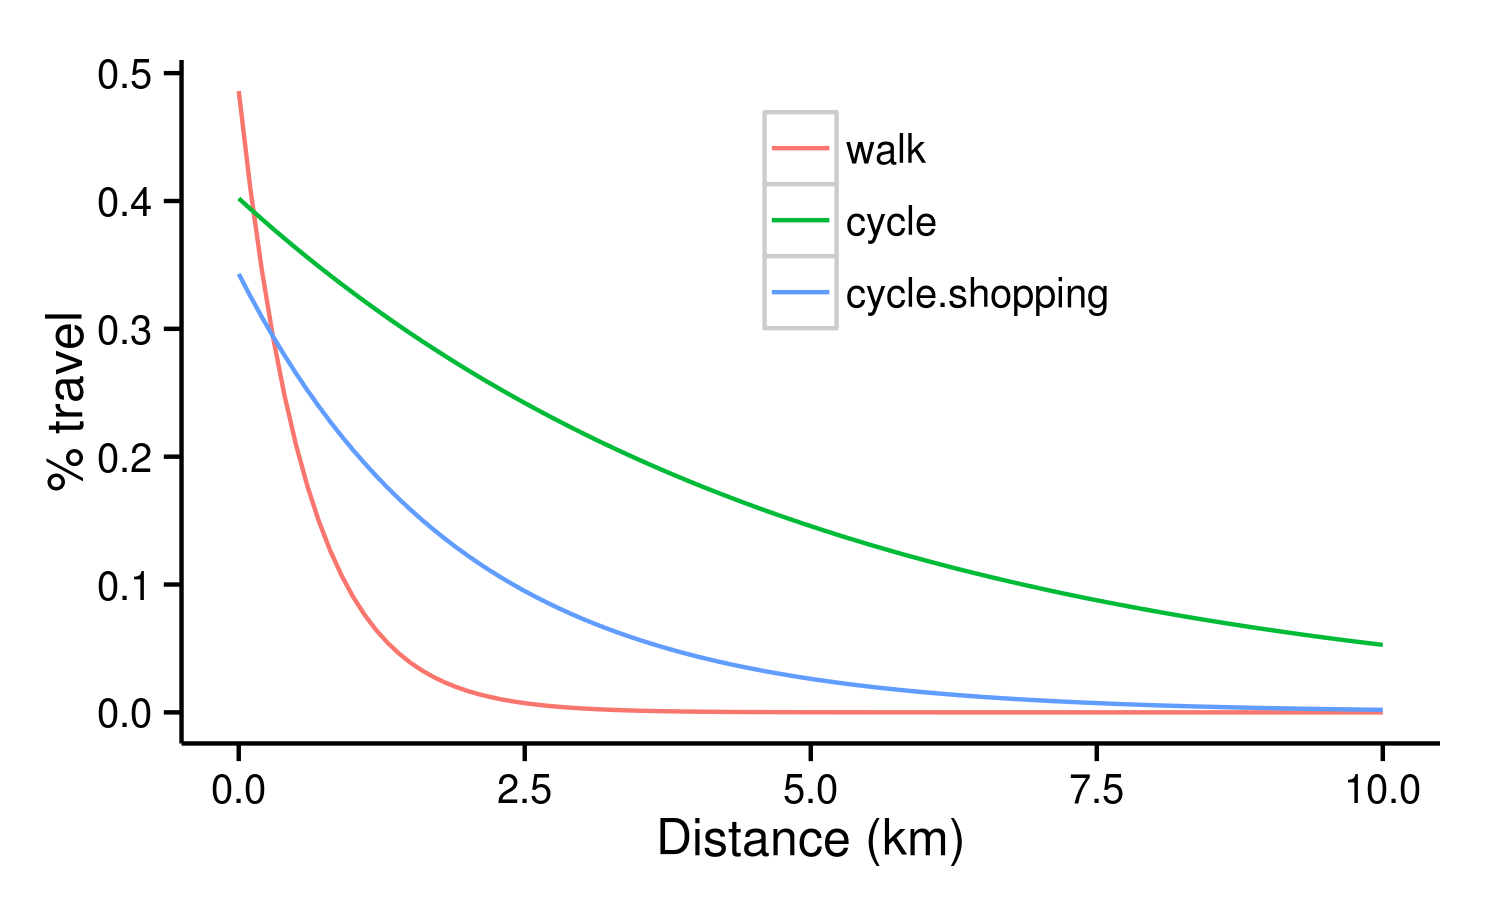
\includegraphics[width = 10 cm]{impedance}}
    \rule{35em}{0.5pt}
  \caption[Proportion of trips by active travel by distance and mode]
  {Proportion of trips made by active travel by distance and mode. Functional form
  from \cref{eimpedance}; parameter values taken from \citep{Iacono2010}.}
  \label{fimpedance}
\end{figure}

In summary, the sustainable mobility literature provides a strong foundation
for investigating energy costs in commuting. The emerging field of
active travel also has a strong interest in energy, although this is rarely
linked to the energy use of motorised modes. Sustainable mobility provides both
a world-view and methodological guidance for the thesis, yet is still only a
minor influence on commuting research overall, as shown in the subsequent section.

\section{Commuting research: individual to national levels} %%% only 1-2000 words
\label{s:commuting}
The energy costs of commuting depend on commuting behaviour.
As \citet[p.~297]{smith2011polycentricity}
put it regarding CO$_2$ emissions from travel to work, they are
``essentially a weighted combination of the mode-choice and travel distance
patterns.'' Understanding
the factors driving travel behaviour is key, therefore, to understanding
energy costs. `Behaviour' can be understood from a range of
perspectives, from the internal workings of the mind to the macro-economic
forces driving the type and spatial distribution of jobs
(\cref{fig:com-pyramid}). This section is structured to
reflect the multiple levels that affect commuter patterns.

Many important factors influencing the decision of whether, how and
how far to travel to work depend on the global economy, which is
largely beyond anyone's control \citep{Eisenstein2011}:
the price of crude oil, industrial
production\footnote{Production of
cars, trains and machinery, for example, is a prerequisite
for the construction and maintenance of transport infrastructure.
}
are all determined outside the sovereignty of any person or even
country, yet these factors, determined by the global economic system,
clearly have large knock-on effects on commuting patterns. National-scale
physical factors also play a role.
The transport network, shifting vehicle fleet efficiencies and the nation's
topography all help determine the ease with which
different commutes are undertaken, and their energy costs.
Large-scale political and
economic processes, such as congestion charges, fuel taxes
and house price gradients also affect commuting behaviour.
Zooming in on the local scale, the strength and nature of the local
economy will decide whether suitable jobs are available locally or
whether one's job search must go further afield.
Community and family ties could both make commuting distances shorter
(by providing support to family and friends searching for work --- the
``home-field advantage'' identified by \citealt[p.~100]{Simini2012}), or longer
(by creating a disincentive for people to move closer to where they
work \citealp{Green-1999-ld-commute}).
At the simplest level, however, the decision to get up in the morning
and commute to work is ultimately made by individuals \cref{fig:com-pyramid}).

\begin{figure}[htbp]
  \centerline{
    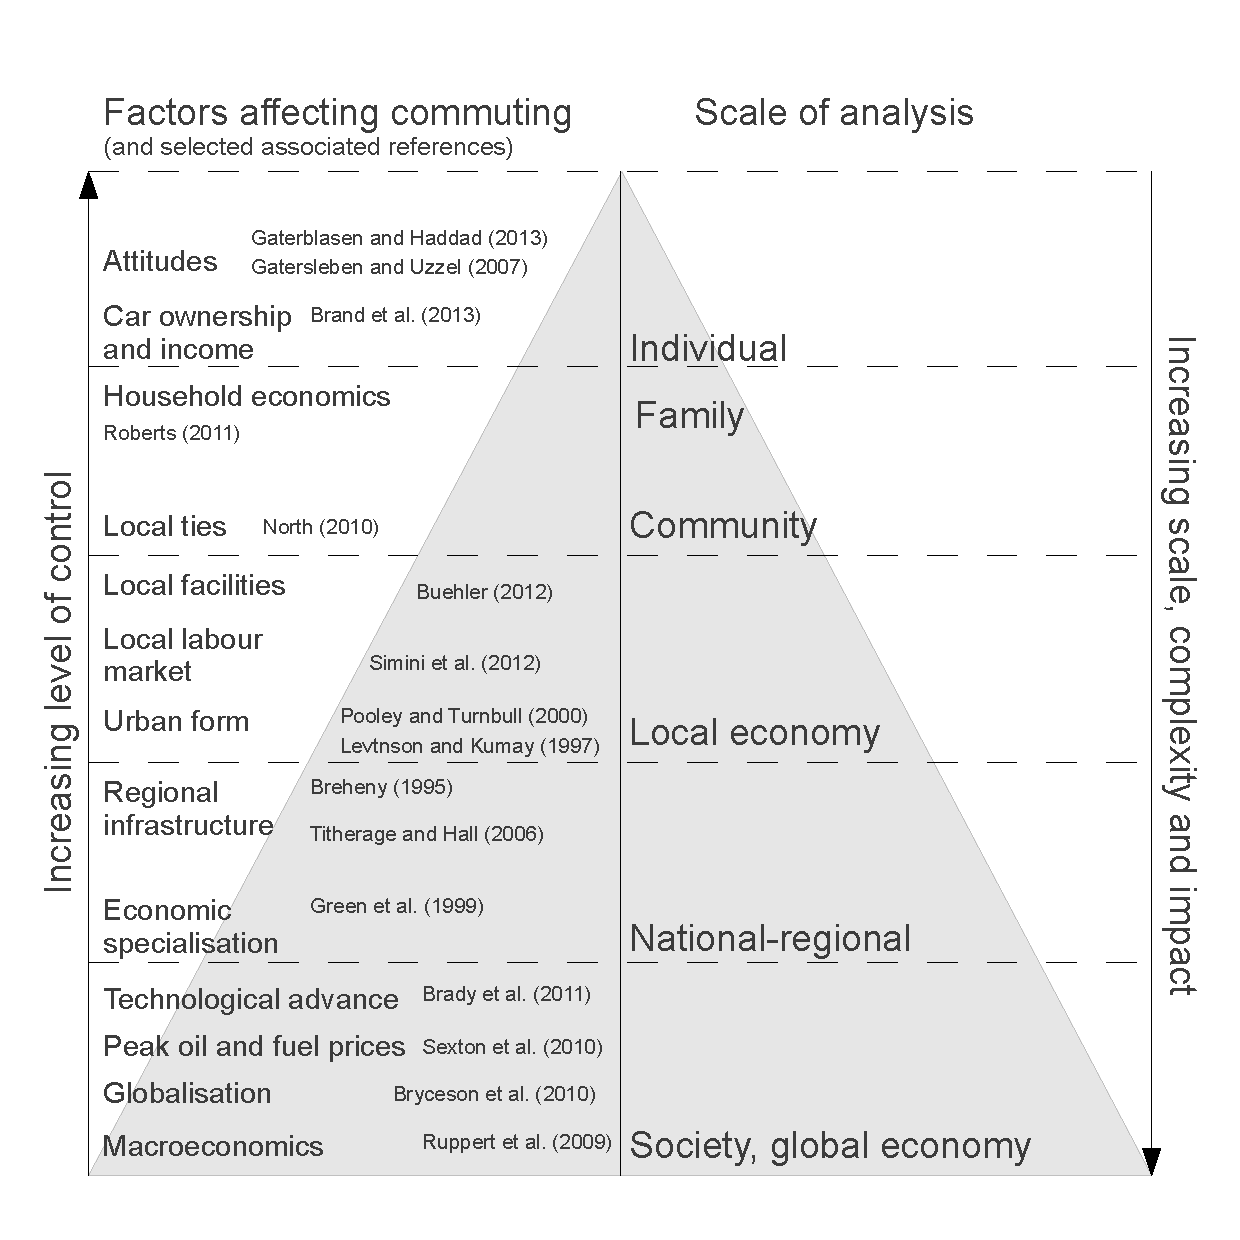
\includegraphics[width = 10 cm]{commuting-research-image2}}
  \caption{Schematic
for organising research commuting research by scale.} %%% could update with methods
  \label{fig:com-pyramid}
\end{figure}

\subsection{Personal factors: psychology, family and community}
As Chris Fisher's story demonstrated (\cref{s:realities}), human beings are not
merely economic machines motivated solely by money. We make decisions based on
a wide and interrelated range of factors \citep{Pinker1997}. Some are instinctive, others
are carefully planned \citep{Kahneman2012}. 
%Within this array of factors
%money tends to play an important role, as do family considerations
%and proximity to friends and one's home town.
While money plays an important role, it is within an array of 
factors along with family considerations and proximity to friends and home.

In some ways, long-distance commuting is the ultimate
manifestation of the conflict between
work and family life. If money were the only objective, people would be far more
mobile, willing to pack their bags and leave to live near better salaried jobs
whenever opportunities arrive. This is obviously not the case:
``job relocation almost always involves a move not only of one
individual's job, but also of his/her household's home and of jobs/schools for other
household members''
\citep[p.~52]{Green-1999-ld-commute}.\footnote{This
decision, to move for personal reasons rather than work,
is also well-expressed in everyday speech:
``I'd much rather
have a crap job and be with Richard than have a good job and be miserable'', as one
person told me (Emma, 2013, personal communication).
}
Over the past 50 years, perhaps due to the perceived social costs
of this upheaval, job relocation has increasingly
\emph{not} led to house relocation, but longer commutes instead
\citep{Green-1999-ld-commute, Nielsen2008}.

This trend has been labelled the `commuting paradox' due to the
seeming irrationality of the decision 
to spend much of one's time travelling to work and back \citep{Stutzer2008},
in face of evidence of negative impacts on well-being \citep{novaco1990objective}.
Approaching the problem at the individual level makes sense:
people are not economic machines,
yet assuming that people make a personal cost-benefit analysis for each
available option allows the powerful tools of microeconomics to be used. Applied to
commuting, each individual would evaluate all work-home (and
hence commuting) options and select the
best \citep{Stutzer2008}.\footnote{Mysteriously,
as the authors of the `commuting paradox' point out, this cost-benefit analysis is often
performed in a less that rational way, leading to commuting costs
(predominantly on unquantified well-being) that far outweigh the benefits
in many cases \citep{Stutzer2008}.
}

Research into commuting at the individual level generally uses psychology
(e.g.~\citealp{van1998social}) or microeconomic theory (e.g.~\citealp{van1999job}) to explain
\emph{why} people choose their commuting behaviours.
Yet the level of analysis is generally weaker when it comes to describing
\emph{how} commuting patterns --- the aggregate pattern of many individual flows ---
are configured and how much energy or other resources these patterns
use relative to other activities.
The relationship between commuting and larger scale processes
is generally not considered in individual level studies, although
there is a move towards more holistic understanding of individuals.
One study that analysed both environmental and psychological
determinants of individual level commuting behaviour found conclusive evidence
(from a sample of 130 university students) that ``cognitive variables play
a more important role in the prediction of active commuting than do environmental
variables'' \citep[p.~9]{Lemieux2009}. Because of the non-geographical nature
of this study and its small sample size, however, it provides little evidence
on the factors related to \emph{aggregate level} variability in commuter flow
patterns. Local, regional and national level studies are needed.

% The psychological literature on commuting sheds some light on
% this commuting paradox.
% \citep{Brand2013}
% \citep{Gatersleben2010}
% \citep{Roberts2011}
\subsection{Behavioural economics and its impacts on commuting}
Behavioural economics seeks to explain a large part of human behaviour in advanced
capitalist societies where making money is often (implicitly or otherwise) seen
as the number one \emph{raison d'etre} of life \citep{Eisenstein2011}.
The underlying assumption that human beings are rational beings
has of course come under attack from many quarters. To take one 
example, ``There is probably no other hypothesis about human behaviour [than
economic rationality] so thoroughly discredited on empirical grounds that still
operates as a standard working assumption in any discipline''
(Anderson, 2000; cited in \citealp[p.~34]{Exel2011-b-ec}). 
Despite these criticisms it is easier to create testable models in economics 
than the social sciences (Perman, 2003).
%Despite
%these
%criticisms, and the fact that the idea of an `economic man' is abhorrent to many
%people's better instincts, a clear advantage of economics over other social
%sciences is the possibility to formulate and test quantitative relationships,
%to evaluate the extent of the models' deviance from reality \citep{Perman2003}.

Indeed, many economists would be quick to point out that the term `economics'
has been conflated with what is in fact `neoclassical economics' in the public
consciousness and in other academic disciplines.
It has been argued that it is only with the recent
focus on money exclusively (instead of the physical reality that underpins
its value) that utility and profit have been conflated \citep{porritt2007capitalism,
Eisenstein2011}.
Clearly, it is not money per se that affects commuting energy costs, but
its indirect influence on behaviour. It is for this
reason that behavioural economics is the
branch of the discipline with most insight into travel to work patterns.
At its most tempered, modern behavioural economics completely accepts that much
of human behaviour follows a rationality other than the profit
motive. Many behavioural economists acknowledge the findings of Nobel
Laureate Daniel Kahneman, neatly summarised in the
book \emph{Thinking, Fast and Slow} \citep{Kahneman2012}, which
explains that humans are servants to both cool rational thought processes
(when `system 2' is dominant) and also to quick-fire decisions based on
spontaneous urges and heuristic reasoning (when `system 1' is dominant). The
caveat in the quantitative analysis underlying economic analyses
becomes ``when humans are acting
rationally, with the objective of maximising profit'' which is only some of the
time.
% (the rest of the time providing a convenient explanation for model errors).

If these limitations are understood, behavioural economics can provide a powerful
framework for explanation. The
framework is consistent with anecdotal evidence about the reasons behind travel
behaviours (e.g.~Chris Fisher's decision not to move to Hereford because
commuting to the Tyrrell's crisp factory would then become too expensive) and
the observed behaviour that people react predictably to price signals.
The framework can also be called upon to explain more general (and less
testable) trends, such as the increasing dominance of the car throughout the
20$^{th}$ century: ``One important reason for the automobile's increasing
dominance in passenger transport is that ... the price of car travel relative
to public transport has largely remained steady while the (system) quality of
car travel has considerably increased relative to public transport''
\citep[p.~149]{Exel2011-b-ec}. % p.149 in the book in case it's different
Far from assuming humans are soulless economic machines,
such explanations, taken as descriptors of aggregate behaviour,
% (not that of specific individuals),
assume citizens are simply careful with their cash.
Such explanations are supported by multiple studies of transport elasticity
(e.g.~\citealp{goodwin2004elasticities}).

\subsection{The local and regional economy}
The idea that localised environmental factors can
influence behaviour patterns has a strong tradition
in geography.
In terms of the impact of local factors on commuting, existing
research has focussed on transport infrastructure, the built
environment,\footnote{The
built environment is defined as ``equipment, facilities or infrastructures in
one's environment'' that influence travel behaviour by \citet[p.~2]{Lemieux2009}.
The built environment can thus be seen as a superset of transport infrastructure,
which includes features such as parks, street lights and even showers designed
to encourage running or cycling to work.
}
topography and local economies, as well as the more abstract concept of
`urban form'.

A common research strategy for exploring these links is to take aggregate travel
behaviour in different areas as the dependent variable and set-up a
multiple regression model to identify which factors can best explain its variation.
This strategy has provided a number of insights into commuting
behaviour and its dependence on geographical factors:
\begin{itemize}
 \item \citet{Buehler2012} ran a logistic regression model and found that
 the provision of showers and bicycle parking by employers (which
 had not previously been included in regression models of commuter behaviour)
 were significantly related to the chances of respondents cycling to work.
 The provision of bicycle lanes and free car parking also had large
 impacts on the odds ratio of a person cycling in the expected
 direction, supporting past literature on the matter. Significantly, this
 study also combined household level variables; it was found that a high number
 of bicycles (and low number of cars) per household member also increased the
 propensity to cycle, as did high income and `white' ethnicity.
 \item  \citet{Titheridge2006} used distance of commute as the dependent variable
 in their study of commuter patterns in the East of England. It was found that
 distance from London, social class and level of car ownership in each ward
 affected distance in the expected ways. Population density, which would
 be expected to be associated with lower energy costs based on the `compact
 city' concept, was positively associated with commuting distance in their model.
 This contrasts the idea that bunched-up living is a panacea for travel costs and
 was explained by \citet{Titheridge2006} in terms of accessibility to transport
 infrastructure.
 \item \citet{Muniz2005} performed a regression analysis exploring the impacts of urban form on
 the `ecological footprint' (which is closely related to energy use) of commuting
 in Barcelona Metropolitan Region. It was found that, for the 163 municipalities
 that constituted the case-study area, low population densities, high `accessibility'
 (which seems to have been defined simply as distance from central Barcelona)
 and high average income all were positively associated with the dependent variable.
 Although this study was conducted at only one scale (it may suffer from the
 ecological fallacy and does not prove causality), the authors concluded that
 factors relating to urban form ``have a greater capacity to explain municipal
 ecological footprints variability than other factors'' \citep[p.~511]{Muniz2005}.
\end{itemize}

Such studies, which use geographical zones as the unit of analysis,
have revealed some of the factors that are closely related to certain commuting
patterns. Some of these, such as propensity to cycle and distance to workplace,
have important energy implications. When the independent variables include
factors over which policy makers have some degree of influence, such as
employers' provision of showers investigated by \citet{Buehler2012}, the
findings can be used to predict changes resulting from new policies. Even in
cases where the independent variables are largely beyond anyone's control ---
such as population density and home-work distances ---
regression analysis can be useful: it can be used to identify anomalies
where commuting patterns differ greatly from what would be expected based on
explanatory variables alone. In these cases, it must be acknowledged that
other processes are in operation, which can lead to new avenues for research.
However, regression analysis used in this way is limited:
causality is not proved; relationships may not hold at different levels of
analysis; and standard regression does not take space into account
(spatially weighted regression can be used to tackle this problem).
Partly to overcome these limitations, a number of other strategies have
been used to explore the geographical determinants of commuting behaviour.

In a study of commuting behaviour in northern Sweden, descriptive statistics
and maps were used to characterise commuter patterns in the region \citep{Sandow2008}.
Making use of the abundant
anonymous spatial microdata made available by the Swedish state, an
individual level logit model, with long or short distance commute
set as the binary variable,
was used to explore the reasons for and impacts of the observed patterns.
It was found that people living in more sparsely populated areas
were more likely to travel far to work than those living in dense areas.
This was as expected (but in contrast to \citet{Titheridge2006}).
The individual level data allowed for the investigation of socio-demographic
variables: education and income were associated with longer commutes.
Interestingly (in contrast to UK data), commuting distance decreases
with every age group above the 16-25 band. Gender differences were also
apparent: men travelled further than women and the impact of marriage and
children on the probability of commuting far was greater on females. Thus
it was concluded that family
commitments ``constrain women to a higher extent than men''
\citep[p.~24]{Sandow2008}.

% Urban form: \citep{Pooley2000commuting}
% \citep{Levtnson1997}
% \citep{North2010585}
% The importance of infrastructure has been noted in a number of studies.
% \citep{Titheridge2006} 

\subsection{National and global considerations}
While regional approaches have tended to focus on detailed sub-regional factors
affecting commuting, national approaches tend to be broader. The large
quantity of data available (albeit often at a high level of spatial
aggregation and low temporal resolution) make the national level
well suited to analysing shifts over time and persistent patterns within commuter
flows. Larger study areas also shift attention towards universal concepts,
that should, in theory, apply anywhere with similar underlying conditions.

In the context of the compact city debate, an individual level regression
model involving 47,000 people across the US was undertaken by
\citet{Levtnson1997} to ascertain the impact of population density on
travel to work distance and time (and hence average speed also). A wide range
of individual and geographical
factors (the latter aggregated at the level of Metropolitan Statistical
Areas (MSA), roughly equivalent to county level in the UK) were
used as explanatory variables. These were
carefully selected based on theory and previous findings. They
included a measure of polycentricity (the number of `activity centres' --- meaning
employment centres --- in each MSA), population growth rate and three variables
to quantify the transport technology in use in each area. It was found that for
car drivers, travel speed and distance were negatively associated with density. Time,
which had received little attention in the compact city debate previously, was found to be
negatively associated  increased residential density up to a certain limit
and then actually increase above this threshold. It was concluded that
this indicates diminishing returns as the density of settlements increased 
if cars are the main form of transport, due to congestion. Public
transport users, by contrast, ``displayed a negative relationship between travel
time and density both above and below the 10,000 ppsm density threshold'',
suggesting that these modes are less affected by traffic (and hence more attractive)
in dense urban areas \citep[p.~168]{Levtnson1997}.

Building on these findings, \citet{Levinson2012}
returned to the question of the factors affecting commute time in US
MSAs with updated datasets and more sophisticated tools for analysis.
It was found that accessibility was the major determining factor of
travel to work characteristics at the MSA level, and had a strong negative
association with average time and mode share of cars. Accessibility
(a slightly refined version of which was used in the final model) was defined,
for given time thresholds, as follows:
\begin{equation}
 a_t = \pi \times \left[ \frac{V_n \times t}{Q} \right]^2 \times p_{emp}
\end{equation}
where $V_n$ is average network velocity, $Q$ is circuity ---
see page xix for definition and \cref{fig:routes} for illustration ---
and $p_{emp}$ is the urban density (measured in jobs per km$^2$). A number of other
mathematical entities were used to define the transport network, the most
influential of which were treeness (roughly speaking, the proportion of the network going to
new places), connectivity (measured in five metrics, from alpha to gamma) and
circuity. The relevance of \citep{Levinson2012} for this thesis is that it
provides strong evidence to suggest key aspects of the journey to work are
influenced by road and settlement factors, and a set of tools for measuring
and assessing the effects of these factors. These techniques are not
used in a model of commuter energy use in the case studies presented in
this thesis, but could be in the future.

% Also at the national scale, \citet{Turnbull2000} used retrospective
% questionnaires to assess the changing nature of travel to work over time.
% The sample size was small 

Commuting has been studied and understood from a wide range of
perspectives. For the purposes of this thesis, insights are taken from economics,
ecology, and transport geography. The first assumes commuters to
be free thinking utility maximisers \citep{Sexton2011}; the second sees humans
as ``mobile, interacting animals'' who ``are no different from our fellow
species'' \citep[p. 40]{Brockmann2012}. Transport geography tends to be
agnostic in its explanatory framework, taking insights from the spatial
structure of transport networks, supply and demand centres, and the physical
environment \citep{Rodrigue2009}.
Interestingly, considering the ubiquity of commuting worldwide, no
research into commuting as a global phenomenon could be found, let alone
systematic comparisons between nations.
This suggests that there is a research gap in the area of international
commuting studies, which may be partially filled by a comparison of the
UK and the Netherlands later in this thesis \cref{sinternational}, as
recommended in the conclusions (see \cref{sfurther}).

\section{Energy use and CO$_2$ in transport studies}
\label{s:energy}
The traditional reasons for interest in commuting and  personal transport
more generally include its links to urban structure, industrial location,
productivity of workers and  quality of life. Economic factors have
tended to be dominant in past research,
but energy use and its environmentally destructive impacts,
predominantly quantified in the form of greenhouse gas emissions,
% \footnote{The term
% `evil twin' is used here because emissions almost always result from
% energy use in transport, yet only the latter is seen as a `bad' thing.
% Energy use can be seen as a good thing when used as a measure of economic
% activity.}
are increasingly becoming a focus for transport researchers \citep{Chapman2007}.
Although CO$_2$ production is a direct result of energy consumption,
depending on emission factors (\citealp{Defra2011}; see \cref{fgco2}), some studies continue to
treat them as separate issues. \citet{Boussauw2009}, for example,
calculate the energy costs of commuting in Flanders, but nowhere does
the paper mention the link to climate change: results are also, in essence,
a map of CO$_2$ emissions due to commuting, relevant to EU targets.
On the other hand,
it is possible and equally valid (if one's primary concern is climate change)
to only quantify CO$_2$ emissions and acknowledge
that the results essentially show energy use \citep{smith2011polycentricity}.

\citet{Simonsen2011} harness the knowledge that energy use
and greenhouse gas emissions are two sides of the same coin to use the
same energy analysis model to quantify both. In their analysis of cars in Norway,
it was found that only electric vehicles powered by renewable
sources (hydro-electric plants in this case, which are bountiful in Norway)
performed well. The approach taken in this thesis follows
\citet{Simonsen2011} in seeing the link
between energy and emissions.
% but takes it even further: the former is seen
Moreover, it is assumed that the former is a close enough proxy of the latter
at the system level that only energy use needs to be
calculated to gain an understanding of
both.\footnote{`At
the system level'
in this context means emissions arising from knock-on impacts of
interventions in the transport system are taken into account.
For example, if rapid uptake of electric cars leads to slower phasing
out of fossil fuel fired power plants, this would constitute
additional emissions at the system level that are not included in
official emissions inventories.
}
This prevents the complexity of having to report two (very highly correlated)
sets of indicators for the energy and emissions impacts. They are assumed to
be essentially the same thing.

Underlying drivers of this interest in energy use in transport and
associated emissions include peak oil and climate
change (\cref{Chapter1}). This attention has led to 
methods and findings directly related to the thesis.
% The work described in the following section is therefore of practical use.
% Describing the methods of, and questions raised by, this body of literature are
% therefore priorities of the subsequent section.
Although there has been a recent proliferation of interest in the contribution of
transport energy use to climate change \citep{Schwanen2011}, the topic
has  received attention, intermittently, over many years. Interest seems to
have peaked during the 1970s,
following the major oil crises of that decade \citep{Greer2009}. Since then the
topic has largely been confined to the following fields:
\begin{itemize}
 \item Urban sprawl:
 the phenomenon of low density housing, also known as suburbia, is highly car
dependent and has attracted attention investigating its impacts on transport energy
use. The antithesis to this is the `compact city'. Investigation of continuum between
these two extremes has led to many insights on the impact of urban form on transport energy use.
\item The energy costs of transport modes: quantifying which modes of transport
use most, and least energy per unit distance, typically per passenger, vehicle or
tonne kilometre: $pkm$, $vkm$ or $Tkm$.
% \item The `compact city' debate, in which the hypothesis that high density
% settlements are more energy efficient, due largely to transport.
% \item Life cycle analysis (LCA) and studies of the relative importance of
% embodied energy in transport systems.
\item The climate impacts of transport, usually quantified through estimates
of the quantity of CO$_2$ directly emitted by vehicles.
% \item The field of `energy and equity', which investigates the impact of
% unequal access to powerful machines for personal travel and social inequalities.
\end{itemize}
Transport and energy use is a broad area of research, so it
is inevitable that not all of it fits neatly into these four categories. A fifth
category, miscellaneous studies on transport and energy, will emphasise this
diversity of approaches, and touch on the interdisciplinary nature of the work.

\subsection{The energy costs of urban form: urban sprawl and compact cities}
The links between urban form and consumption of fossil fuels (primary energy)
have been of interest since at least the 1940s, especially amongst utopian town
planners \citep{Steadman1977}. Of the various types of urban form under
consideration, from the fictional `City of Efficient Consumption'
\citep{Goodman1947} to the `compact city' \citep{Breheny1995}, none have
received more critical attention than that of urban sprawl \citep{Marshall2008}.
Urban sprawl has long been identified as an energy intensive settlement
pattern, with social and environmental knock-on effects: ``Urban sprawl not only
consumes more natural ecosystems and has a higher cost per unit of development
in both money and materials, but once completed it requires higher inputs of
energy and generates more air and water pollution'' \citep{Bormann1976}.

Such statements may seem obvious, yet without evidence questions about
the extent of the
problem, and how to mitigate it, remain unanswered. This is a key motivation
behind methods which seek to measure aggregate energy use over space, and
provide breakdowns of how much energy is used where, and insights into why.
% (Example of overall energy use)
One implicit assumption underlying much of this research is that
energy use is \emph{the} defining
variable of a settlement and hence requires most attention.
This reasoning was stated explicitly by
\citet{Marique2012}, who note that despite the primacy of the transport sector
in driving up energy use in sprawling suburbs, ``transport energy consumption
is rarely taken into account'' (p.~1). In response to this negligence, the authors
quantify the average transport energy costs in four settlements, based on travel
statistics. Their analysis shows commuting to be the most
important determinant of transport energy consumption in Belgium. Commuting
consumes more than double the amount of energy (4000 to 6000 kWh/p/yr) 
than the next largest transport energy user (trips to school)
\citep{Marique2012}. These findings lend support to the topic of this thesis and
encourage further analysis of energy use in personal travel overall.

Despite the use of census data, \citet{Marique2012} present their findings only
at high levels of aggregation, for entire settlements. The \emph{distribution}
of energy consumption within the areas is not considered. Nor are the
\emph{types} of people responsible for high energy use for commuting. These
gaps in their research suggest more detail would be welcome: providing a method
to calculate the energy costs of commuting at lower geographies that is capable
of providing breakdowns of energy use at the individual level would constitute
a step forward for this research.

\subsection{The energy costs of different transport modes}
The relative energy use of different ways of travelling per unit distance
or time has been of interest
to researchers at least since the 1800s when \citet{tredgold1835practical}
was taking measurements from railway engines to ascertain their coal
consumption. A more universal approach to energy use in transportation
was taken by \citet{Gabrielli1950}, who characterised the energy performance of
different modes, for given speeds and loads. This model included jet fighters,
helicopters and even a horse, as well as more traditional vehicles such as
cars, bicycles and trains. Although largely unnoticed by the academic
community (it has been cited 11 times according to Google Scholar), this
paper was seminal in its approach to comparing widely varying forms of
transport, and the findings still largely hold today (although efficiency
gains have been made) \citep{yong2005price}. An updated analysis, which uses
a simpler energy performance metric, kilogram-metres per Joule, multiplied
by speed ($kg*m^2/J/s$) applied the method
to a wide range of modern vehicles, confirming the relatively poor energy
performance of cars in comparison with trains and bicycles (\citealp{Radtke2008},
\cref{fgabrielli}). This is a recurring theme in \cref{Chapter5}.

\begin{figure}[htbp]
  \centerline{
    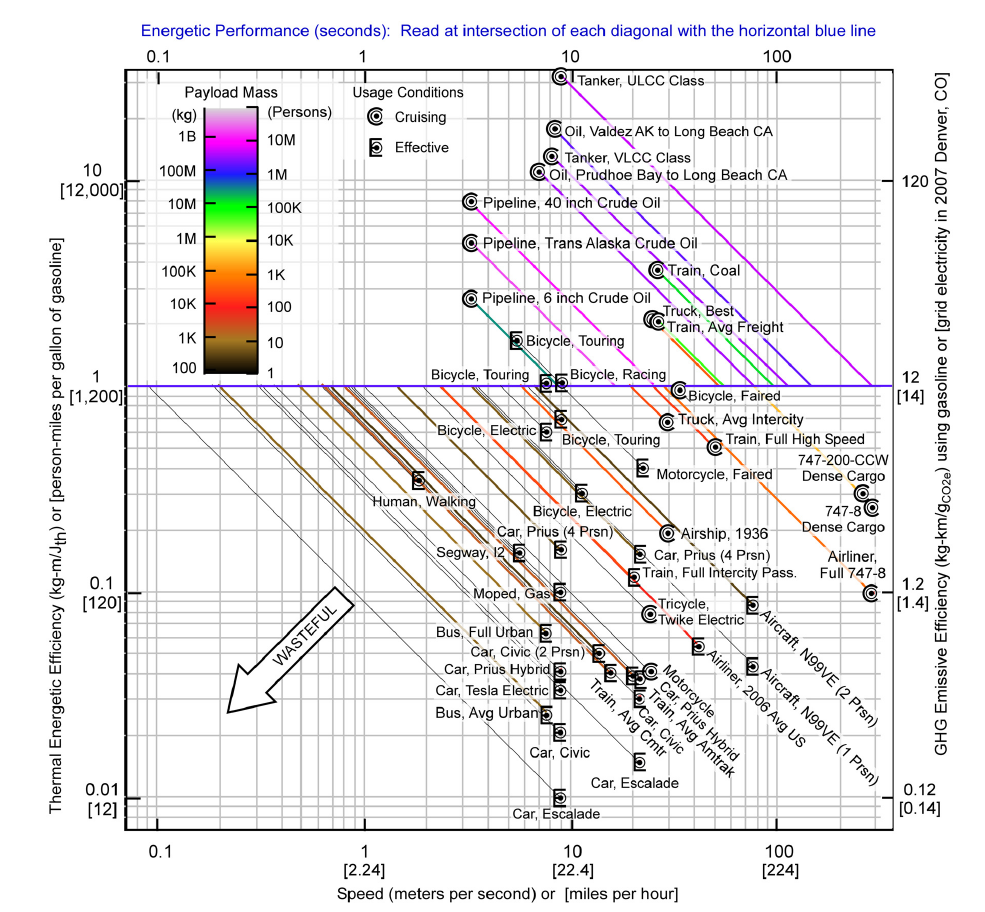
\includegraphics[width = 13 cm]{gabrielli}}
  \caption{Energy performance of different modes, from \citep{Radtke2008}.} %%% could update with methods
  \label{fgabrielli}
\end{figure}

\citet{Gabrielli1950} and their successors made large advances in understandings
of the relative energy costs of widely different transport modes.
It is therefore surprising that methods and findings stemming from this
work are not more frequently used in transport studies.
One limitation of the research area is that it omits indirect energy impacts from
the analysis.
This is problematic because vehicle and infrastructure manufacture obviously
require large amounts of energy: inclusion of direct energy costs only
``might lead to serious faults in estimating environmental impacts of new
infrastructure or modal shift policies'' \citep[p.~23]{Wee2005}.
A pioneering paper that sought to overcome this issue quantified
both the direct and indirect
energy costs per unit kilometre of the main US modes of personal travel shortly
after the 1973 oil shock \citep{Fels1975}.

In hindsight, Fels' research seems to have stood at the beginning of a
research area, dedicated to assessing the wide-boundary energy impacts of
personal travel. Key papers in this area include \citet{Lenzen1999}, who used
updated versions of Fels' early methodology to calculate the total energy and
emissions impacts of the Australian transport system and  \citet{Ramanathan2000}
used a new method (`data envelope analysis') to investigate
the relative energy costs of Indian road and rail transport.
% The analysis was
% novel in that it took into account both freight and passenger transit in
% the analysis, leading to the finding that rail efficiencies have continuously
% improved, while road transport efficiency has plateaued since the late 1980s.
Another group of researchers have researched essentially the same
issue, but with different methodologies and terminologies
(the `well-to-wheels' approach) from the
life cycle analysis (LCA) perspective (e.g.~\citealp{wang2002fuel};
see \cref{sfuelem}).
Because research rooted in LCA tends to be
concerned with emissions rather than energy use per se, it is
of slightly less relevance to this thesis.
Surprisingly, there seems to be
limited overlap between the well-to-wheels approach and the aforementioned
system level energy use studies.
Despite the activity of these research areas, 
there has been limited uptake of system level energy
cost estimates in transport studies overall. Direct emissions and
their climate impacts have received more attention.

\subsection{The climate impacts of transport}
Since 1985, when Professor James Hansen of NASA's Goddard centre testified
to the US congress about the threat posed by climate change, there has
been a growing concern about the issue from all quarters, including the media
\citep{Boykoff2007}. While media insistence on `balance' seems to have actually
led to bias in climate change reporting, providing excessive coverage to contrarian
views \citep{boykoff2004balance}, academia has largely risen to
the challenge in practical terms. A multitude of articles has been written on how to
reduce emissions in everything ranging from catering \citep{gossling2011food}
to the Indian cement industry \citep{kumar2010environmental}.
Acknowledging that transport is responsible for roughly a quarter of emissions,
researchers in the sector have been no exception.
Modelling scenarios of future change proposing new policies
for emissions reductions are now common themes in the transport literature
(see reviews by \citealp{Chapman2007} \citealp{ross2010analysis}).

Without delving further into this large and diverse body of literature,
a few generalised criticisms of it can serve to
highlight where improvements can be made. It is acknowledged that
these observations do not apply to all research into
transport and climate change. The reason for voicing these concerns,
summarised in the bullet points below, is that they
help focus attention on areas within the field lacking in
coverage.
% Their consideration has contributed to the energy approach
% to commuting presented in this thesis in the following ways:
\begin{itemize}
 \item Transport and emissions studies have tended to focus exclusively on
 direct emissions, to the detriment of understanding of the system level or
 `embedded' emissions resulting from transport policies,
 such as road construction and vehicle
 manufacture \citep{Lenzen1999, Wee2005}.
 \item Because of the focus on the national level, papers in the area
 could be argued as offering little in the way of support to local and regional transport
 planners. This is an important oversight because local and regional level
 transport planners vastly outnumber national policy makers (in staff, if not
 in terms of political influence).
 \item The various scenarios of the future often appear to be overly academic,
 arbitrary and unrealistic. This is
 problematic because impenetrable models and scenarios
 may prevent engagement and interaction with the
 possible futures presented, by either the public at large or policy makers.
 To overcome this issue, participatory models
 such as that published online by the Department of Energy and Climate Change
 (\href{http://2050-calculator-tool.decc.gov.uk/pathways/11111111111111111111111111111111111111111111111111111/primary_energy_chart}
 {\color{blue} 2050-calculator-tool.decc.gov.uk}) have been advocated
 \citep{fulton2012exploring}.
\end{itemize}

Despite these issues, this thesis fits within the field: although the emissions
benefits are not calculated explicitly, it is not a large jump from energy
costs to emissions (CO$_{2eq}$ output
would be easy to estimate, based on the
emissions factors present in \cref{Chapter5}). The efforts to estimate
system level energy costs of different modes presented in the same chapter
are aimed at overcoming the focus on direct emissions alone, prevalent in the
transport-climate change literature. Regarding scale, in some ways it makes
sense that many of the studies in the area operate at a large scale
because climate change is inherently a global issue.
The problem is that there is an excess of studies that operate only at the
national level, with relatively little work focussing on larger or smaller geographical
unit of analysis. The methods
presented in this thesis are well-suited to smaller geographical unit areas, although
they can also be applied to nations (\cref{Chapter6}).
The methods presented in this thesis are not participatory (unless one is
willing to learn to code in R and apply it to spatial microsimulation!).
However, effort has been made to make the code and data underlying the
models as accessible as possible.\footnote{See
\url{http://rpubs.com/robinlovelace}, which contains links to
reproducible result, via sample code and data. Github has also
been used to make some experimental analyses available.
}

% \subsection{Assessing the energy impacts of political intervention} \label{spintervention}
% !!!

\section{The energy impacts of commuting} \label{sdisciplines}
The intersection between these two study areas, each large in its own
right and with substantial interaction, is surprisingly small.
As described in the previous two sections, major advances in understanding
commuting behaviour and energy use in transport have been made.
The problem is that these insights into commuting are often not
translated into energy use
estimates.\footnote{This step is in fact
relatively straightforward, once the energy use of different modes is well-known
(\cref{Chapter5}).
}
Or, conversely, existing estimates of energy use of different modes and
other personal variables are not combined with readily available
commuting statistics. The energy cost of commuting is not a
`pure' research area, in the sense that it relies on combining data from
sources that often are not linked.

The study that most closely fits the title of this section
was based on aggregated census data from Flanders. Without relying on
regression analysis  or sophisticated statistics \citet{Boussauw2009}
provided a detailed account of the factors linked to areas with
high and low average commuter energy costs. By mapping average
energy consumption per person per day (ranging from almost zero
to above 30 kWh/p/d) for small administrative zones, the impacts of
modal split (minimal), distance (``paramount'') and urban morphology and
infrastructure on energy use for commuting were determined. These are new
and important findings that need to be tested in other countries
and at different scales
before they are accepted as `universal' relationships that can form the basis of
policies worldwide. It was concluded that
``the energy performance of the transport system is an important approximate
indicator for the sustainability of a spatial structure'' \citep[590]{Boussauw2009}.
This observation was a major motivation for the subject matter of this thesis.
%!!! requote this elsewhere???
The political implications of the research are wide-ranging: the prevailing
focus on mode-split in Belgium (and in many other countries, including the
UK where uptake of cycling has become a major political issue) seems to be misguided.
Governments should instead focus on enabling their citizens to live closer to their
place of work.

\citet{Boussauw2009} did not provide `further research' type conclusions. However,
the arguments made throughout for a greater role for energy-based metrics of
transport system performance and sustainability clearly imply that more
research measuring energy use in commuting is needed. The paper therefore
provides a strong intellectual foundation on which this thesis is built.
The methodological guidance was limited as the analysis was quite simple.
From this was taken the importance of seeing method as a means to an end,
rather than an end in itself, an issue that has been debated in academia for
many years. 
%% surely there's another study that fits here???!!! looking good though.

% \subsection{Energy use and transport poverty} 
% One of the earliest investigations into the
% links between energy intensive modes and social and economic disadvantage
% was Ivan Illich's book \emph{Energy and Equity}
% \citep{Illich1974}. Since then, the causes identified by Illich for growing
% inequalities in personal mobilities and `power' --- the ever increasing speed
% with which the economic elite can travel, powered by fast cars --- has grown
% and plateaued. % would like to re-add this, at some point!!!
% 
% \citep{Sustrans2012}. %

% Commuting is an inherently spatial activity, as its purpose is % valuable!!!
% to transport people from A, their home to B, work.
% This, combined with readily available official data sources
% on commuter flows, make the phenomenon well suited for study
% within the field of transport geography. This field aims
% to explain ``the socioeconomic, industrial
% and settlement frameworks within which transport
% networks develop and transport systems operate''
% \citep{Hoyle1992modern}. %%% Citation added.
% The focus on explanation rather than mere description
% makes the field a rich source of ideas about \emph{why} transport systems,
% and more specifically commuter patterns, are the way the are.
% Plough on with examples from the literature

% Commute minimisation \citep{Buliung2002}
% 
% The concept of `activity space' is another key concept
% used by transport geographers... \citep{Buliung2006}.

% Transport geography is inherently multidisciplinary,
% and has contributed to wider debates started in other fields.

% \citep{Marique2013}
% 
% Despite the theoretical bias in Transport Geography noted at the beginning of
% this section, there have been substantial methodological contributions to the
% analysis of commuter patterns. The methods to evaluate different
% types of estimate of route distance (GPS, shortest route algorithms via
% GIS and straight-line distance) presented by \citep{Stigell2011}.
% Their result that self-report distance is the least reliable provides
% useful background for assessing the reliability of the input data
% used in this PhD. (Census data are straight-line distances by
% postcode, the survey data is self-reported route-distance.)

% \subsection{Non-academic contributions to commuting research}
% The above research is based predominantly in the realm of academia, written by
% University scholars and published in academic journals. The advantages of this
% `academic model' of research are clear, and have been implemented throughout
% this thesis. These include:
% \begin{itemize}
%  \item Traceability of sources of information --- hence the inevitable in-text
% references and lengthy reference lists that accompany academic research.
% \item Reproducibility of results --- academic writers must clearly state what
% they have done, why and report the results in a way that could be replicated,
% given the correct conditions.
% \item Impartial writing style --- academic writing is different from more
% creative styles, in that ideas must be ordered logically and artistic elements
% minimised in favour of clarity \citep{oshima1997introduction}.
% \end{itemize}
% 
% Because commuting is such an important part of the daily routine for millions
% of people, it has received much attention from outside academia too.
% Literacy has improved worldwide and
% opportunities to publish (most recently with the emergence of paperless
% E-books) have multiplied, so it is impossible to hope to have encountered even
% a tiny fraction of the totality of material written about
% commuting.\footnote{This
% could be interpreted as an additional advantage of the academic publishing
% model: it is relatively cohesive self referential compared with the tangled
% mass of non-academic writing. The latter is not ordered into neat searchable
% databases that is connected by a formal reference system in the same way that
% academic papers are.}
% What follows therefore is a concise summary of `lay' works on
% commuting that have been discovered, usually by coincidence, and that
% contribute information or understanding to the topic energy costs of commuting.
% 
% \citet{Orloff2002-60-second-commute} provide a self-help guide on telecommuting
% for those wishing save time and money.

While \citet{Boussauw2009} were writing from the perspective of transport
geography, the primary concern being spatial variation of energy costs,
the issue of energy costs has also been tackled from the perspective of
mainstream economics. \citet{Sexton2011} set out to
test a hypothesis: that the 2008 sub-prime mortgage crisis was triggered
by high liquid fuel prices. The mechanism for this was commuting energy costs ---
those who live closer to their place of work were found to be less affected.
This was shown through a number of maps illustrating the change in average
house prices over space. Areas furthest from employment centres had the greatest
falls, whereas house prices in more central locations were relatively unaffected.
This study demonstrates the importance of energy costs of commuting,
not just in abstract terms of environmental impact or global resource depletion,
but in terms of direct impacts on peoples' lives. No attempt is made to
replicate the economic methods used by \citet{Sexton2011} in this thesis.
However, \cref{svul} was heavily influenced by the paper. It takes from
\citet{Sexton2011} the need to assess potential future impacts of high oil prices
on different social groups.

\section{Commuting and energy use research: tools of the trade}
\label{s:tools}
The previous section illustrates that energy use in commuting can be seen in 
at least two different ways: a dependent variable influenced by geography, or
an explanatory variable affecting household expenditure.
Many other ways of looking at commuter energy use are possible and each
would suit different methods for describing and explaining
energy use. While research methods
and explanations can be closely bound
together,\footnote{\citet{Simini2012}, for
example, harness a vast commuter dataset covering the USA to support their
general numerical model of commuting: the model to a large extent
contains explanation implicitly.
}
different research methodologies
can also be used to investigate the problem from a single perspective.
For this reason the methods discussed below
are considered separately from the other sections of this literature review.
Theories are hypotheses about how the world \emph{should be}, based on
experience, concepts and intuition, while
the methods help uncover facts about how the world \emph{is}. This is the
standard model of science, which progresses by falsifying ideas which fail to
explain observed reality, and leads to the acceptance of systems that have most
explanatory power \citep{Popper1959}.

In some ways, this scientific approach
can be seen as a tool of the trade in itself: it provides a framework within
which competing theories can be impartially compared, and provides a mechanism
to discard ineffective explanations, `sorting the wheat from the chaff' in terms of
ideas about the world. For this reason the scientific method, as it has been
intermittently applied to research into commuting, is discussed as the primary,
and most broadly defined, tool of the trade.
% Spatial statistics, %(which have
% %only emerged since large spatial datasets became available during the 20)
% travel diaries, interviews,
Visualisation techniques have progressed alongside advances in data availability
and analysis are considered as a key method in the research area.
Finally, the `data deluge' precipitated by the
widespread adoption of handheld GPS devices and traffic monitoring technology
is briefly considered. This source of information may, one day,
rival official commuting statistics as a dataset from which to understand the
energy costs of work travel.

\subsection{`Scientific' approaches to energy and transport}
Science is a contested concept but has undoubtedly had a large impact on
methods of researching energy use in transport. Rather than be restricted
to Popper's narrow definition of science (as any knowledge that can produce
falsifiable hypotheses), the literature is more usefully seen as falling into a continuum,
ranging from ``scientific'' on the one side, to ``not scientific'' on the
other. This is not to make a value judgement about which research is `better'.
(Indeed, one could argue that commuting is not a research area
that is amenable to true science at all, due to the complexity of human decision
making and the impossibility of controlled experiments.) It is simply
to say that some methodological approaches borrow more heavily from the
formalisation of theory and emphasis on quantification and testability of
science than others. 

A well-established `scientific' theory about commuter patterns is the gravity
law. The law is falsifiable (and has been falsified on numerous occasions!)
because it predicts the number of trips ($T$) from location $i$ to location $j$
using the following formula:
\begin{equation}
 T_{ij} = \frac{m_{i}^{\alpha} n_{j} ^{\beta}} {f(r_{ij})}
\label{eq:gravl}
\end{equation}
where  $m_i$ and $n_j$ are the populations of the start and
destination settlements respectively, $r$ is the Euclidean or `straight line'
distance of the
journey, and $\alpha$ and $\beta$ are parameters to be calculated based on
evidence. The functional form of the denominator is open to interpretation,
making the gravity law more of a modelling framework. Proponents have
claimed that the
framework can predict commuter flows between two settlements, once the
functional form of \cref{eq:gravl} has been learnt.

This is quite a sweeping statement. Clearly, the model cannot be correct all
the time because it is deterministic. It can, however, produce a
sufficiently close fit with reality, across a number of transport flows, that it
has become ``the prevailing framework with which to predict population movement,
cargo shipping volume and inter-city phone calls, as well as bilateral trade
flows between nations'' \citep{Simini2012}. The gravity law has been applied to
commuting on a number of occasions with results pertinent to energy use.
\citet{gargiulo2012} presented a spatial interaction model based on the
gravity law. It was configured using a single parameter ($\beta$ in \cref{eq:gravl}),
and was used to calculate the probability of individuals travelling
from their home to workplace zones. Although no energy implications were investigated
by \citet{gargiulo2012}, the model could be used to
predict energy costs via trip counts between different zones.
In a related paper, \citet{Lenormandplosone2012} presented results of
a model that calculates commuter flows between zones about which the number
of incoming and outgoing commuters is already known. From this input dataset
could be estimated the flow between each zone pair, to a high degree of accuracy.
The authors tested their results against the radiation model and
found that theirs ``yields significantly better results''
\citep[p.~6]{Lenormandplosone2012}. It is to
this radiation model, another scientific approach to commuting, 
that attention is directed below.

The gravity law has been recently criticised by
\citet{Simini2012}, who proposed an alternative that they refer to as a
`radiation model'. In this model, the flow rate between two zones is defined
probabilistically. The average flux is estimated as follows:
\begin{equation}
\langle T_{ij} \rangle = T_i \frac{m_{i} n_{j}} {(m_i + s_{ij})(m_i + n_j + s_{ij}) }
\label{eq:radi}
\end{equation}
where $s_{ij}$ is defined as the total population living within a circle, the
centre of which lies in the centroid of zone $i$ and the radius of which is
the distance between zones $i$ and $j$. Thus, the greater the population
living within the commute distance, the lower the estimated flow rate.
This is key to the radiation model: it accounts not only for the characteristics
of the origin and destination zones, but also the surroundings.
Not only does this model have strong theoretical underpinnings, it also
performed well against commuting data from US counties: the flow between
each county pair was predicted with a high level of accuracy, based solely
on the population of each. The potential utility of this model in
energy applications is considerable: it is highly flexible so could be used in its
raw state, before adding refinements to explain the impact of infrastructure.
Also, the concept of impedance (introduced towards the end of \cref{sactive})
could be used to create modified versions of \cref{eq:radi}
for each commonly used form of transport. With both modifications in place,
such a model should be able to predict the energy implications for commuters of both
new settlements and new infrastructure.

% Another `scientific' model for understanding commuter flows was presented
% by \citet{gargiulo2012}. In this modified version of the gravity law, with a single
% parameter ($\beta$ in \cref{eq:gravl}), each commuter is allocated a workplace
% probabilistically, using randomised sampling. The model is slightly less
% simple than that presented by \citet{Simini2012}, but could be used in the same
% way as a predictor of energy costs via modal split and distance.
% The stochastic interpretation of the gravity law has also been used by
% \citet{Lenormand2011} to simulate commuter flows.
% There are many other spatial interaction models based on the gravity law to
% predict flow rates. A challenge is knowing which one is most suitable for commuting,
% suggesting a need for cross-comparisons. My hypothesis would be that the new radiation
% model provides the best starting point, and this could be tested by UK commuter
% flow data. 

Another area where the mathematical formalisation of theory has been useful in
energy-transport research is in the creation of future scenarios.
\citet{Kohler2009} used an agent-based model to create scenarios of behavioural
change and uptake of new transport technologies between the years 2000 and
2050. The novelty introduced by their model was use of different `agents' ---
people (`consumers') interacting with higher level `niches' and `regimes' to
determine the final outcome. The modelling framework is flexible, and allowed
for complex dynamic behaviour to be simulated. A downside of the model was
that it depended heavily on user input to set initial parameters. These
parameters were set in a
``scenario storyline of a successful transition'' \citep[p.~2988]{Kohler2009},
in which hydrogen fuel
cell cars become widely available by the 2040s. Clearly, this scenario of the
future is more the product of human imagination than the scientific method,
and the future may take an entirely different technological path than that
imposed by the authors.
However, the sophistication of the approach shows that scenario creation
can go beyond simple population models \citep{Lovelace2011-assessing} or
user-defined snapshots of the future \citep{Akerman2006}.

\subsection{Visualisation methods}
People tend to think visually and often lack the concentration or ability
to read through long verbal descriptions or understand mathematical formulae.
For this reason visualisation is important:
``A picture really can be worth a thousand words, and human beings are very adept
at extracting useful information from visual presentations'' \citep[p.~4]{kabacoff2011r}.
A list of some of the main visualisation techniques for representing
is therefore timely at the outset, to provide context and justification
for the use of figures in this thesis:
\begin{itemize}
 \item Choropleth maps are very common in geographical commuting research,
 providing an insight into the areas where particular behaviours are most
 prevalent. A minor difference between the maps used in most previous
 research and this is the use of continuous colour scales in this thesis,
 instead of bins for communicating energy costs (see \cref{Chapter6}).
 This can be problematic if a distribution is highly
 distorted by outliers, in which case bins would be preferable, but can provide
 additional information to the reader if neighbouring zones have values at the
 opposite ends of a single colour bin.
 \item Geographical flow maps, with thickness of lines joining origin-destination
 pairs proportional to the flow (e.g.~\citealp{Smith2009}).
 This technique is employed in \cref{s:workdes} to illustrate the important of
 knowing \emph{where} commuters are travelling to for local transport decisions
 that consider commuter energy use. Often these maps lack direction, however,
 leading to the use of arrows or asymmetries in lines being added
 (e.g.~\citep{Nielsen2008})
 \item On-line visualisations have become increasingly common as software such
 as Processing, OpenLayers (for maps) and an R package called Shiny have become
 increasingly available and user friendly. Although no on-line visualisations
 have been created for the main thesis, `Google Fusion Tables' and `Geoserver'
 options were considered to make the results more
 accessible.\footnote{A presentation
 on this topic was given by the author at the FOSS4G (Free Open Source
 Software for Geospatial) annual conference 2013.
 The slides can be viewed
 {\color{blue} \href{http://robinlovelace.net/visualisation/open\%20source/conferences/presentation/2013/09/22/foss4g-presentation.html}
 {online}}.
 }
\end{itemize}

% \subsection{Travel diaries}
% 
% \subsection{Interviews and participant observation}

\subsection{Harnessing the `data deluge'}
The increasing market penetration of hand-held GPS devices, in dedicated
packages \citep{Oliver2010} and more recently embedded within `smartphones'
\citep{Gong2011}, has lead to an `overabundance' of spatial data which must be
filtered, prioritised, ordered, sorted and analysed to provide meaningful
results.\footnote{%%%%%%%%%%%%%%%%%%%%%%%%%%%%%%%%%%%%%%%%%%%%%%%%%%%%%%%%
%%%%%%%%%%%%%%%%%%%%
This was the topic of
the Sixth International Workshop on ``Geographical Analysis,
Urban Modeling, Spatial Statistics'', held in Salvador de Bahia, Brazil,
June 2012. The problem neatly summarised on the conference's web-page:
``During the past decades the main problem in geographical
analysis was the lack of spatial data availability. Nowadays the wide diffusion
of electronic devices containing geo-referenced information generates a great
production of spatial data. Volunteered geographic information activities (e.g.
Wikimapia, OpenStreetMap), public initiatives (e.g. Spatial Data
Infrastructures, Geo-portals) and private projects (e.g. Google Earth, Microsoft
Virtual Earth, etc.) produced an overabundance of spatial data, which, in many
cases, does not help the efficiency of decision
processes''
(\url{http://www.unibas.it/utenti/murgante/geog_an_mod_11/index.html}, accessed
February 2012).
%%%%%%%%%%%%%%%%%%%%%%%%%%%%%%%%%%%%%%%%%%%%%%%%%%%%%%%%%%%%%%%%%%%%%%%%%%%%%%%%
}
This `data deluge' is still in its early stages \citep{Bell2009}, yet is
already having an effect on approaches to geospatial data analysis
\citep{Jiang2011}. The data analysed come from more
conventional sources (primarily the Census and official surveys). However, it is
important to be aware of the potential for this research to contribute to
knowledge about commuter energy use.

% Studies using GPS tracking devices worn by study participants can measure
% location, velocity, and route planning (). This research is still in its
% infancy yet has already shed light on commuting (get to the point - lit review
% to the max!)

\section{Concepts in energy and commuting} \label{skeyconcepts}
% A wide range of research has been presented in this chapter, and some of it
% may seem unrelated under first impressions.
The diversity of research on energy and commuting is great, yet within this
body of work lies a set of concepts that appear repeatedly. The purpose of
this short section is to summarise some of these ideas
and to help tie together the literature reviewed in this chapter.
The first two will act as points of reference in later sections.
% Summaries of
% these concepts will be quantified where possible, as an explanation of the
% assumptions made in future chapters, and to provide material for the discussion
% of the results.
% !!! Provide summary table at end with range ???
\begin{itemize}
 \item \emph{Circuity ($Q$)}: This is the ratio of network distance to Euclidean
distance
between two places \citep{Levinson2009}:
\begin{equation}
 Q(i,j) = \frac{dE(i,j)}{dR(i,j)}
\end{equation}
Circuity is important due to its impact on energy use \citep{Levinson2012}
and because other metrics of the transport network's performance can be
derived from it \citep{Barthelemy2011}.
Circuity impacts energy use because in highly circuitous
networks, more energy must be expended to go the same distance. In addition,
if circuity is low for energy intensive modes (e.g. the route
between settlements joined by a motorway), these modes will be preferred.

Circuity is also important practically:
the distance bins used to disseminate UK census data measure Euclidean distances,
whereas the actual distance travelled depends on network distance: to
calculate energy use, the circuity factor $Q$, must be used to translate
between the two. The second reason for circuity's importance
is that other useful metrics of transport system performance can be derived from
it. These  include the \emph{accessibility} of a location
 (how circuitous is the average route to that place), and the
\emph{global efficiency} of the network. These additional concepts
which grew out of the understanding of circuity have strict mathematical
definitions and could be used to quantify the impact of network
structure on scenarios of the future, including the likely resilience of
different parts of the travel network under scenarios of natural disaster
\citet{Barthelemy2011}. This is a research area with great potential for
the future. In this thesis, however, circuity is the only quantitative
description of the transport network to be implemented: in \ref{scircuity}
circuity is described as a mechanism to map the Euclidean
distances reported in the census to the route distances reported in survey data.

\item \emph{Efficiency ($\eta$)}: Efficiency is an important concept in
transport and energy studies. As with its everyday use, often its meaning
is not strictly defined in the transport literature. ``This is not an
efficient use of time'' is a typical use of the term, meaning that the
benefits (outputs) are low considering the time input. 

Regarding energy use, the meaning is the same, although the mathematical
definition allows for precision:
\begin{equation}
 \eta = \frac{E_{out}}{E_{in}}
\end{equation}
Where $E_{out}$ is energy that is useful (e.g. electricity), and $E_{in}$ is
the primary energy input (e.g.\ calorific content of petrol). Of course, the
definition of `useful' is open to interpretation\citep{Patterson1996}, leading
to various measures of efficiency, ranging from pure thermodynamic definitions
\footnote{The efficiency of electricity production, for example.}
through to
economic-thermodynamic definitions\footnote{For example, the efficiency of
freight transport can be defined as tonne-kilometres per unit energy input
(tkm/MJ) \citep{Simongati2010}. This hybrid economic-thermodynamic measure is
more commonly expressed as fuel economy of freight, its reciprocal
(MJ/tkm).},
to purely economic definitions\footnote{This is measured as the proportion of
an activity's monetary cost that is spent on energy --- the proportion of bus a
bus fare that goes towards diesel costs, for example.}. The concept of
efficiency --- and related concepts of fuel economy and energy
intensity --- is well established in research on the energy requirements
of freight transport \citep{Kamakate2009}. It has rarely been used to compare
the performance of different transport modes, however \citep{Fels1975,
Lovelace2011-assessing}.

A general principal of energy efficiency measures is that they should reflect
the purpose of the process they describe \citep{Patterson1996}. In commuting,
the transport of \emph{people} is the aim, so the commonly used fuel economy
metric (l/100 km) is not an appropriate measure of the  performance of the
system \citep{MacKay2009}. The preferred energy metric for this research is
therefore energy intensity:
\begin{equation}
 EI = \frac{MJ}{pkm}
\end{equation}
The energy intensity of passenger transport modes are described
(after a large body of evidence on the matter is considered) in \cref{sfinal}.
In everyday speak when transport modes are described as `efficient' people
are generally referring to energy intensity rather than thermodynamic
efficiency. Following this convention, `efficiency' when used in this thesis
also generally refers to energy intensity.

In terms of the energy costs of commuting, the preferred metric is the average
energy costs per commuter per two-way commuter trip (MJ/trp).
This is similar to the units of kWh/p/day used by \citet{Boussauw2009},
but the denominator is the number of commuters in this study, not the number
of people (making the results impervious to variable unemployment rates) here.
To translate MJ into kWh, multiply by 3.6.
The energy per trip results are presented in \cref{Chapter6} at a variety of scales.

\item \emph{Resilience}: this is measure of a system's capacity to function
after enduring external shocks \citep{Holling1973}\footnote{The seminal
definition of resilience is that it is ``a measure of the persistence
of systems and of their ability to absorb change and disturbances'', while
maintaining their functionality \citep[p. 14]{Holling1973}.
}.
Despite its origins in Ecology, the concept is applicable to any complex
system, and is especially relevant to the relationships between the
economy and the natural environment \citep{Holling2001}. In the sustainability
literature, the term is rarely quantified (see \citealp{Bridge2010}). However,
there has been progress in defining resilience mathematically for 
networks, which could theoretically be used to calculate the impacts of
large collapses, such as blackouts, or, by corollary, failure of the transport
network \citep{Barthelemy2011}. At present however, this quantitative branch of
the resilience concept lacks empirical application. The term is harnessed to
discuss the long term sustainability of commuter systems and their capacity to
function in the event of oil shortages.

\item \emph{Inertia}: in its original physical definition, inertia is the
characteristic of mass by which it ``endeavours to preserve [itself] in its
present state, whether it be of rest or of moving uniformly forward in a
straight line'' \citep[p. 73]{Newton1848}. In the context of transport systems,
inertia is used to describe `lock-in' to the current
transport system in the short term, and its resistance to change:
``Transport systems and urban lay-outs have great inertia and take years to
change'' \citep[p. 365]{Chapman2007}.
\end{itemize}

\section{Summary of the literature} \label{sc2sum}
This chapter has highlighted the range of methodologies and disciplinary
diversity of studies investigating the energy costs and
greenhouse gas emissions of personal travel.
The sustainable mobility paradigm provides a useful label that can be applied to
much of this research, differentiating it from the traditional supply-side
approach bemoaned in the opening quote. The majority of the literature in
transport and energy is not concerned with such high level discussion, however,
generally preferring to `let the facts speak for themselves'. The area of
study is quite new (except for a flurry of work following the
1970s oil shocks, exemplified by \citet{Fels1975}), perhaps explaining why
geographical studies into energy use for transport are still
largely descriptive (e.g.~\citealp{Marique2013, Boussauw2009}), content to
explain spatial variability intuitively rather than with the use of a
predictive model. This thesis takes a similar approach and is primarily
concerned with \emph{describing} the variability of commuter energy costs
at geographic and individual levels. This appears not to have been done
before in the UK.

Transport and energy use has been investigated from a wide range of disciplinary
perspectives, from psychology and economics through to engineering and physics.
This is because energy use depends not only on the efficiency of transport
technologies, but also the behavioural factors that determine how they are used.
Following this diversity, the research presented in this thesis is also
explicitly multi-disciplinary: claiming allegiance to any one discipline
would likely be at the expense of another, potentially 
hindering understanding of the complexity of factors at work.

The energy costs of transport, and their underlying causes, have been explored at a
range of different scales. Individual factors including family
and career commitments have an important role to play, but whether or not
these can be modelled using quantitative data from surveys remains to be seen.
At the regional level, geographical factors influencing energy use in transport
have been explored with reference to the `compact city' hypothesis. CO$_2$
emissions and energy studies have tended to operate at large national or
regional levels, despite the fact that most transport planners and other decision
makers implement policies (especially in the realm of active travel) at the
local level. This suggests a gap in the literature and highlights the need
for energy and transport studies focussed more locally. Moreover,
because the factors affecting commuting behaviour operate at many levels,
there is a need for further development of methods that allow factors operating
at individual and geographical levels to be taken into account simultaneously.

% and have focussed
% on description and scenario modelling rather than explanation.
% Despite the fact that most   A research gap





% \section{Conclusions: knowledge gaps and research directions}


%  \citep{Ballas2005}
 % Literature review

% Chapter 3

\chapter{Spatial microsimulation and its application to transport problems}
\label{Chapter3}
% \lhead{Chapter 3. \emph{Spatial microsimulation and % Definitely worth writing
% % as a stand-alone paper
% its application to transport problems}} % Write in your own chapter title to set
\fancyhead[RO,LE]{Chapter 3. Spatial microsimulation} %2side
\fancyhead[RE,LO]{\thepage}

\begin{quote}
\textit{The modellers' task is to predict how people and organisations will live
in
`good' and `sustainable' cities; how the infrastructure will, or should, grow;
and how activities and traffic flows are, where appropriate, best managed,
priced and regulated.}
\flushright{\citep[p.~3]{Wilson1998-past}}
\end{quote}

Microsimulation can have variable meanings depending on whether you are a
geographer, transport planner, or economist
(see \citealp{Ballas2005b, Liu2006, Bourguignon2006} for examples).
This chapter reviews existing work that uses individual level data and modelling
techniques to investigate transport and related problems.
It also introduces static spatial microsimulation, a particular type of
microsimulation that is central to the thesis. The method enables
individual level and geographical variation in commuting behaviour
to be analysed in tandem. Operational definitions, based on
established research, are important for clarity, repeatability and to
show how the work presented here builds on past research. A number of key terms will be
frequently used throughout the thesis, so this chapter begins with
definitions.
This is followed by an overview of the history (\cref{s:history}) and current
state of the art (\cref{s:sotart}) of the technique as it relates to transport
issues such as travel to work.

As implied in the quotation above, transport does not happen in isolation from
other phenomena. It is part of the complex web of social relations, the environment,
infrastructures, economics, policies and decisions
that define modern settlements. From this
perspective, spatial microsimulation for transport applications is just one
branch of a long-standing tradition of urban modelling
\citep{Wilson1970, batty1976urban, batty2007cities}.
Other branches include dedicated transport modelling techniques
(e.g.~\citealp{SATURN2012}), integrated land-use transport  models
\citep{Wegener2009} and agent-based approaches \citep{Gilbert2008-abm}.
These research areas are related to the thesis and in some cases have
the potential to build on its results. In this chapter they
are grouped together under the broad term `urban modelling' and
discussed in \cref{s:urbanmodel}. The final section of
this chapter (\cref{s:bigdata-gps}) summarises the literature and
explains how it relates to methods implemented in the thesis.

% considers new research directions that have
% been made possible by  the availability of `big data' harvested from the
% internet or alternative sources such as GPS loans to survey participants.
% New approaches are already
% making substantial contributions to understandings of personal travel.
% Harnessed correctly, these new data sources have the potential to improve the
% energy use estimates resulting from microsimulation models and shed insight into
% the validity of assumptions made. %%%!!! Not any more!

\section{Definitions: what is spatial microsimulation?}
\label{s:defs}
\emph{Microsimulation}, as its name suggests, refers to the modelling of
individual units --- e.g.~people, household, companies --- which operate in a
wider system. Used in this sense, the term originates in economics, where it
signified a theoretical turn away from aggregate level analyses and towards a
focus on individual behaviour. ``This shift of focus, from sectors of the
economy to the individual decision making units is the basis of all
microsimulation work that has followed from Orcutt's work''
(\citealp[p.~145]{Holm1987}; see \cref{s:digirev} for further reference to
this work). Microsimulation overall therefore has a wide meaning, from
individual vehicles in a transport model \citep{Liu2006, Ferguson2012}
to the inventories of
competing firms over time \citep{Bergmann1990a}.
The term has a narrower definition in this
thesis, however, that is more concerned with modelling the distribution of
behaviours of individuals over space than over time. This thesis is predominantly
concerned with only one subset of microsimulation: spatial
microsimulation, modelling the distribution of individuals over
space. Within the category of \emph{spatial} microsimulation, different types
can be specified (\cref{types-msim}).

\emph{Spatial microsimulation} of the static kind can be formally
defined as
follows: the simulation of individual level variables within the geographic
zones under investigation \citep{ballas2003microsimulation-30-years, Ballas2007simb}.
The models that perform this operation have also
been referred to as `population synthesizers' \citep{Mohammadian2010}. This
term is useful in the context of transport applications, because small area
micro-population generation is only one stage of a wider process of
individual level transport modelling (\citealp{Pritchard2012}; \cref{f:msim-schematic}).

\begin{figure}[h]
 \centering
 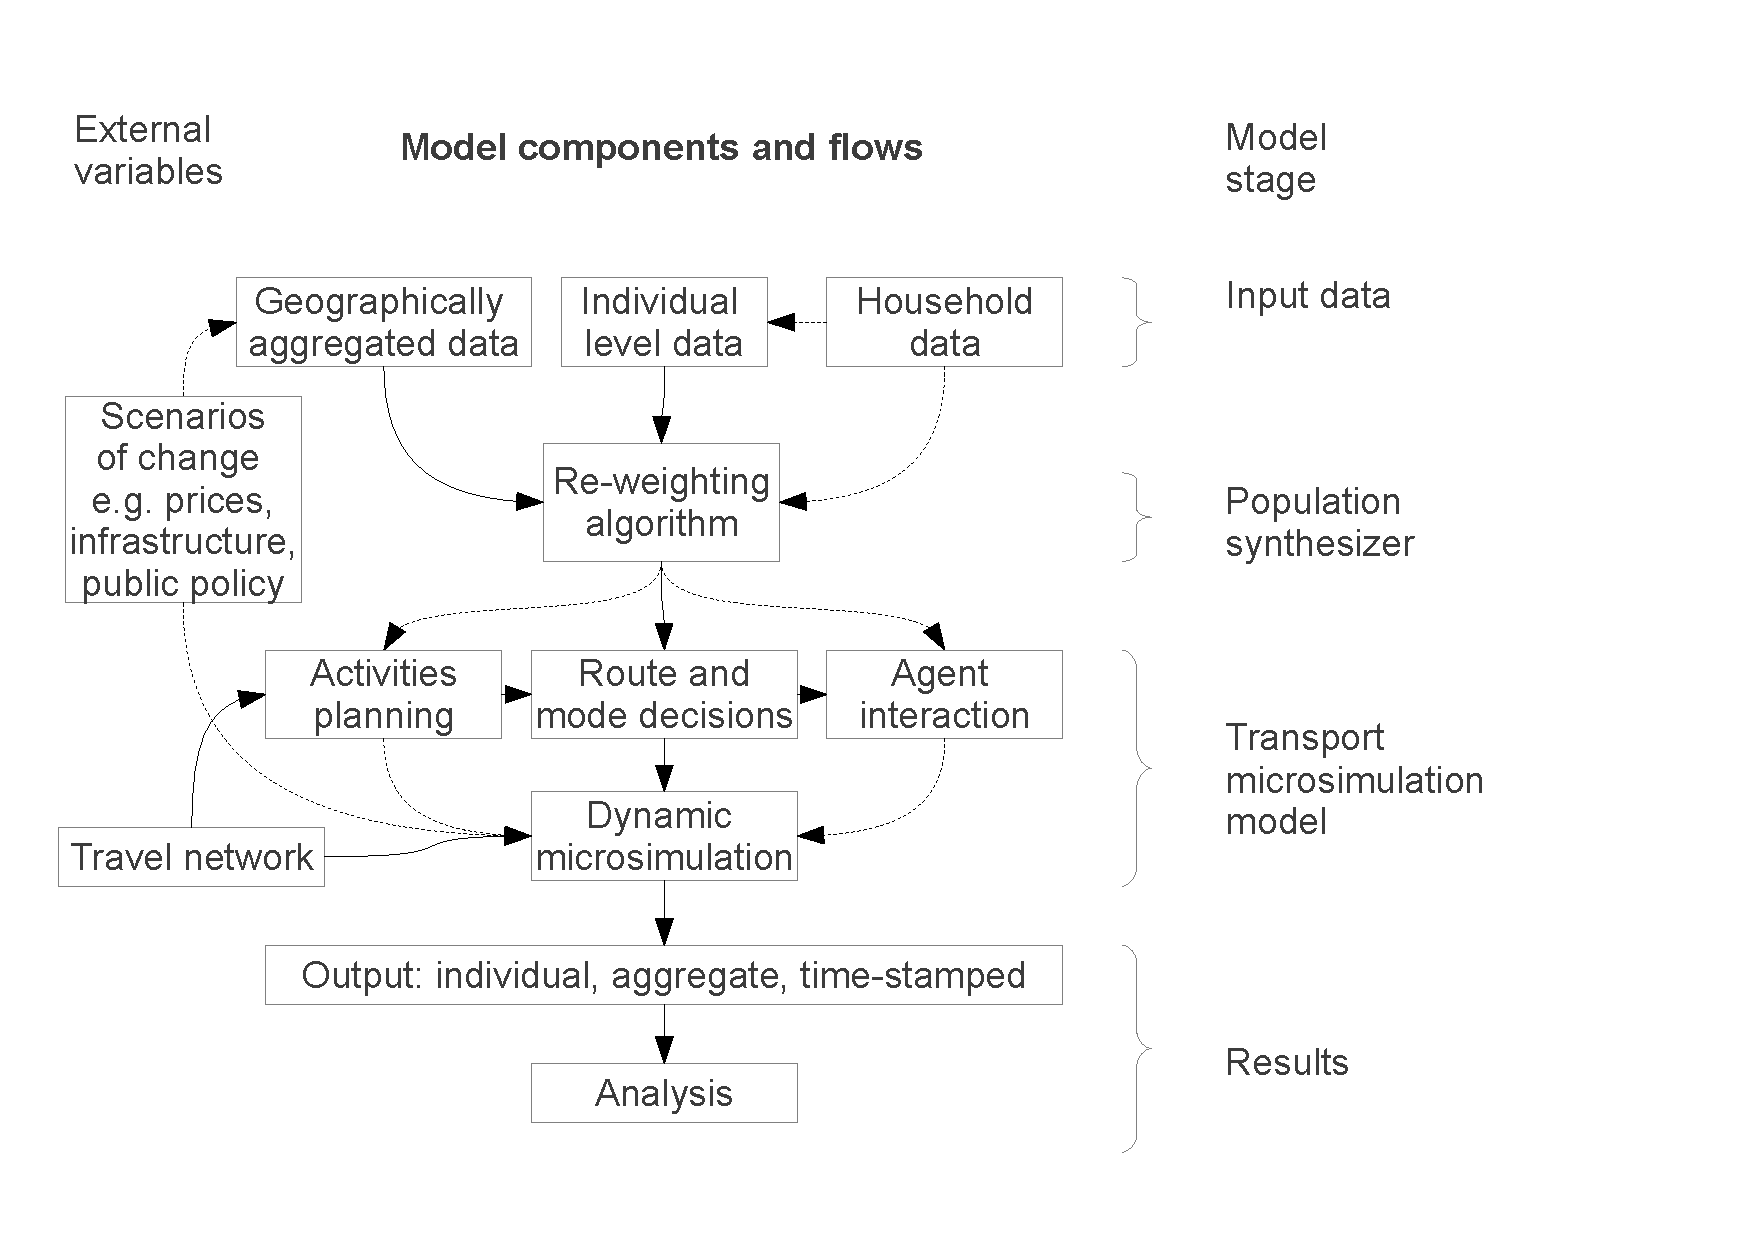
\includegraphics[width=16 cm]{msim-schematic}
 \caption[Schematic a transport simulation model]{Schematic
of the components of a complete transport simulation model such as
TRANSIMS, after \citet{nagel1999transims} and \citet{Mohammadian2010}.
This thesis is primarily concerned with the first two stages.}
 \label{f:msim-schematic}
\end{figure}

During static spatial microsimulation individuals are sampled from a non-geographical
dataset via  reweighting, based on what have become known as `constraint variables'
from early combinational optimisation work \citep{Williamson1998}. The key
feature of these variables is that they are present in
both individual level and geographically aggregated data
sets.\footnote{Constraint
variables must be categorical variables (such as
`male', `age: 16 to 19' or `works 0 to 2 km away from home')
that are shared between the micro level data and
known geographical aggregates, usually from the census.
Continuous variables have not been used in the microsimualtion
literature reviewed, although they could theoretically be
used, by constraining variables' spread, skewness
and central tendency.
}
% The next 2 paras are taken from ints3.tex
\Cref{f:msim-schematic} shows the technique in the wider context of
transport modelling. Spatial microsimulation
here refers to only the top two stages in the diagram. It represents a
computationally small but important (for social analysis at least)
part of the wider simulation process. It is important to clarify this
distinction, as the meaning of `spatial microsimulation' can be ambiguous.
It can refer
either to the process of population synthesis
\citep{chin2006regional, Ballas2005c, Hynes2008},
or the entire urban modelling process that
builds on the spatial microdata \citep{Wegener2011}.
Spatial microsimulation here refers to the former case. The results could
thus be harnessed as inputs into more complex dynamic models in which
individuals interact with each other and other entities in a wider urban model.
The terms \emph{dynamic spatial microsimulation} or \emph{agent-based models}
will be used to refer to the wider modelling process.

Static spatial microsimulation (generally and henceforth referred to simply as
spatial microsimulation) involves sampling rows of
survey data (one row per individual, household, or company) to generate lists of
individuals (or weights) for geographic zones that expand the survey to the
population of each geographic zone considered. The
problem that it overcomes is that most publicly available
census datasets are aggregated, whereas individual level data are generally
much more detailed \citep{ballas2003microsimulation-30-years}.
The ecological fallacy, whereby relationships found at one level are 
incorrectly assumed to apply to all others \citep{Openshaw1983}, for example, can be tackled
to some extent using individual level data allocated to geographical zones
\citep{Hermes2012a}. This `spatial' or `small area' microdata is the output
of spatial microsimultion.

Despite its ability to output geolocated individuals,
spatial microsimulation should never be seen as a
replacement for the `gold standard' of real,
small area microdata \citep[p.~4]{Martin2002}. From the perspective of social
scientists, it would be preferable for governments around the world to follow
Sweden's example and release such small area microdata anonymously. However, this
prospect is unlikely to materialise in the UK in the short term,
adding importance to the process
of model validation. In any case, the experience of spatial microsimulation
development and testing can help prepare researchers for the analysis of real
spatial microdata. Also, the technique's links to modelling make spatial
microsimulation useful for investigating the impacts of policy or other
changes in the real spatial microdata \citep{Holm1987}.
The method's practical usefulness (see \citealp{Tomintz2008})
and testability \citep{Edwards2009} are beyond doubt.

Assuming that the survey microdataset is representative of the
individuals living in the zones under investigation,\footnote{The suitability
of this assumption is further discussed in \cref{Chapter8}.} the
challenge can be reduced to that of optimising the fit between
the aggregated results of simulated
spatial microdata and aggregated census variables such as age
and sex \citep{Williamson1998}. These variables are often
referred to as `constraint variables' or `small area constraints'
\citep{Hermes2012a}. The term `linking variables' can also be used, as they
\emph{link} aggregate and survey data.
Based on the literature, the technique seems to have been used for five main
purposes, to:
\begin{itemize}
 \item model variables whose spatial distribution at the aggregate level is
otherwise unknown (e.g.~\citealp{Ballas1999}).
\item estimate the individual level distributions of variables within small
areas about which only aggregate counts or summary statistics are known (e.g.
distance travelled to work)
\item understand the spatial distribution of discrete behaviours
(such as visiting `stop smoking' centres --- \citealp{Tomintz2008})
and thus the likely local level effects of policy change \citep{Ballas2001}
\item project future changes at the local level, based on past trends
\citep{Ballas2005}
\item provide a foundation for agent-based models, which rely on
discrete individuals \citep{Ballas2007simb, Pritchard2012, Wu2010}
\end{itemize}
The main purposes of spatial microsimulation here are
related to bullet points one
and two above. However, elements from each will be harnessed at some
point.
In essence, spatial microsimulation merges individual level data (a list
of individuals, each with their own ID) with geographical data (a list of
zones, each with its own ID). It therefore relies on two types of input data:

The \emph{microdataset} is the individual level data from which individuals are
weighted or probabilistically selected. It is referred to as the survey
dataset \citep{Wu2008} or simply as `individual data' \citep{Simpson2005}.
The input microdata should be as representative of the zones being studied as
possible\footnote{For
example, the date of survey data collection should be
close to date of at which the zonal data was collected. Also, the survey data
should preferably be from the same geographic region as the zones under
investigation, or at least weighted so that individuals from the region under
investigation are more likely to be sampled \citep{Ballas2005-ireland}. An alternative
way of making the survey dataset more representative is to preferentially
sample individuals from areas with the same classification as the 
their zone being modelled.
}
and sufficiently diverse. %%%!!! More here!

The \emph{constraint variables}, `small area constraints' or `linking
variables' are the aggregate level variables that link the zonal and individual
datasets together. They must (for current methods, at least)
be categorical and the categories in the two
datasets must be the same (re-categorisations may be needed).

\emph{Target variables} are the variables that spatial microsimulation seeks
to estimate. Typically they are not reported at all at the small area level
(e.g.~income), leading to the term `small area estimation' being used
to describe spatial microsimulation when it is used to estimate the
average values of unreported variables for small areas. But spatial
microsimulation can also be used to simulate the distribution of variables that
are already known. Thus, although distance is a constraint variable in
our model, it is also in some ways a target variable: 
little is likely to be known about its distribution within each distance bin. 
Finally, counts of interaction
variables (e.g. male, over 50,
high social class and car driver) are typically not reported from the Census.
These can therefore also be referred to as target variables. Overall,
target variables is the term given to the information targeted for
estimation by the spatial microsimulation model.

\emph{Reweighting} is the process by which individuals are assigned a weight
for each of the zones under investigation. \citet{harland2012} provide
an overview of the methods available for this process, which is
also known as `population synthesis'. The higher the weight for a
particular area, the more representative is the individual of that area,
compared with the rest of the survey dataset. Combinational optimisation
and deterministic reweighting 
are the two main methods for reweighting \citep{Hermes2012a}.

\emph{Combinatorial optimisation} \index{combinatorial optimisation} is an
approach to reweighting that uses repeated randomised sampling to
repeatedly select individuals from the survey microdataset and allocate them to
zones \citep{Williamson1998, Voas2000}. Based on the fit between simulated
and known aggregate counts after each
iteration, the parameters of the resampling algorithm can be adjusted (e.g.~via
simulated annealing).

\emph{Deterministic reweighting} refers to non-random methods of allocating
weights to individual-zone combinations \citep{Ballas2007simb, Tomintz2008}.
Iterative proportional fitting (IPF)
is a widely used deterministic reweighting algorithm and is used in the
spatial microsimulation model throughout. Whole cases
are generated using integerisation.

\emph{Integerisation} is the process by which integer weights are generated
from the non-integer weight matrix (see \cref{s:integerisation}).

\emph{Cloned individuals} \index{cloning} are rows in the survey microdataset
that have been replicated more than once in the spatial microdataset for a
particular area \citep{Smith2009}.
The cloning of individuals can be represented by an integer
weight above one, or simply by repeating identical rows multiple times. In
practice these two forms of representing data are interchangeable; the latter
takes up more disk space \citep{Holm1996} but may make certain types of analysis
easier.


\section{The history of spatial microsimulation}
\label{s:history}
This section outlines the history of spatial microsimulation. It would
be easy to repeat past work here.\footnote{Readers interested in a
comprehensive history of the field are directed towards
\citet{Ballas2009-sage}.} To avoid this, the focus is on
developments that influence the way spatial microsimulation
is and can be used for transport applications. These include:
\begin{itemize}
 \item the influence of location on individual behaviour via
 transport costs 
 \item the question of data vs theory driven approaches
 \item converting a spatial microdataset into a behavioural model
 \item the impact of rapidly advancing computers and data sources
\end{itemize}
These themes are present throughout the section, which is ordered
roughly chronologically.

\subsection{Pre-computer origins}
The theoretical origins of spatial microsimulation stretch back to before the
turn of the 20$^{th}$ century. It was only with the emergence of large scale
data sets, methods of analysis and conventions of mathematical notation that
quantitative analysis of variables that vary over time and space could actually
occur \citep{Ballas2009-sage}.
Despite (or perhaps partly because of) the absence of these pre-requisites for
the analysis and simulation of large populations at the individual level, much
progress was made in thinking about how individuals behave within environments
that vary in predictable ways over space before computers were available.
Consideration of travel costs (which were much higher before most
people travelled by motorised modes) was integral to both Christaller's
central place theory and Von Th\"{u}nen's concentric agricultural zones.
Lacking reliable data with which to test their ideas, the
early quantitative geographers had to make do by
developing theories based on personal observation.
Some of these theories are still influential today \citep{Clarke1985}.
Ideas developed in the pre-computer age can be seen as the theoretical
forefathers of the microsimulation models of transport behaviour, and frameworks
for interpreting the results, that are in use today.

One explanation for the greater theoretical focus of pre-computer work
is that empirical data seldom fit into any neat model and therefore
distract from explanation.
This point was made as early as the 1970s, accompanied by the
warning that the
accelerating deluge of new datasets and quantitative methods was leading some
to conflate quantification with theory \citep{Wilson1972-theoretical}.
Much theoretical work has been done since this cautionary tale. Yet the
same problems of being blinded by new information (to the detriment of
deductive thinking) face modellers now, probably to a greater extent.
This, in combination with the fame enjoyed by early theoretical geographers
(as opposed to more recent empirical geographers who modified or
rejected their work), goes a long way to explain why researchers continue to cast back to
the pre-computer age for theoretical
insight. Two of the early theories that are most pertinent to
simulation of travel patterns are Von Th\"{u}nen's, on the
spatial distribution of
agricultural activity and Christaller's central place theory.

Von Th\"{u}nen's work in the early 1800s is a seminal example of this early
theoretical thinking. His model of concentric zones of agriculture was
described verbally and in the evolving language of mathematics but rarely tested
on real data \citep{Moore1895-thesis}.\footnote{For
example, ``although [Von
Th\"{u}nen] claims that his advantage over Ricardo consists in his ability to
reduce the co-operation of capital to terms of labour, the validity of that
claim has not been tested'' \citep[p.~126]{Moore1895-thesis}.
} 
Von Th\"{u}nen's work exerts a strong
influence, even in the 21$^{st}$ century (e.g.~\citealp{lankoski2008bioenergy}) 
due to its use of geographically defined variables, strictly 
defined assumptions and extensibility \citep{sasaki2003agent}. 
The approach describes individual units based in
Cartesian space, that can be seen both as discrete zones, or as
a continuous variable (as an input into the cost of travel)
\citep{Stevens1968a}. The model's insight into the variability of
individual level behaviour depending on their zone of habitation can therefore
be seen as a direct precursor to spatial microsimulation models. These also
seek to describe the characteristics and behaviour of individual units living in
geographical zones.
%%%!!! Please god give me time to make
% A general version of the Von Thunen model and place it on github -> rinseage
% Rinse this section; concise; go back if needed!!!

Walter Christaller's central place theory of the 1930s provided an integrated
theory of spatially variable behaviour (primarily shopping) and the location of
settlements of varying sizes \citep{matthews2008geography}. Based on the
assumption of a continuous and even geographical space ready for urban growth,
the theory proved fertile for hypothesis testing and extension to other sectors.
% based on increasingly complex mathematics .
Following Von Th\"{u}nen, Christaller
attempted a `scientific' explanation of the behaviour of individuals based on
where they live. The mechanistic nature of the approach has since been
superseded by more advanced and probabilistic models
yet central place theory continues to influence
many areas of spatial modelling \citep{Wilson1972-theoretical, Sonis2005,
Farooq2012-integreted}. Applied to commuting, the theory provides a ready made
model about where people travel to work: the settlement that can provide the
best pay, minus travel costs. Of course, both pay and travel costs vary greatly
depending on a number of individual and geographic variables that cannot be known
in every case. However estimates can be made (even in the absence of now
readily available data) and applied stochastically. 
This theoretical approach has subsequently helped
explain spatial distributions in travel to work patterns, using models based on
Christaller's ideas \citep{Tabuchi2006-commuting-costs}. Christaller was
a major advocate of explaining theories in
mathematics: ``the equilibrium of the location system ... can only be
represented by a system of equations'' (Christaller, 1933; quoted in
\citealp[p.~35]{Wilson1972-theoretical}).
More recent research suggests that urban systems are rarely in equilibrium
\citep{batty2007cities}. In any case, Christaller provided a hypothesis about
why some settlements grow more than others, attracting more people, trade and
commuters.
% Whether or not this statement is true,
% and its potential applicability to commuting patterns, is
% discussed in \cref{Chapter8}. % No, it's not!
More prosaically, Christaller's theory also helps explain why
long-distance commuting appears to be more common into large cities than small ones
(see \cref{Chapter6}).
% !!! REallly? + maybe more precisely located cross ref.

The preceding discussion provides only a small snapshot of pre-computational
spatial analysis, based on two influential thinkers. The
focus was on deductive reasoning, rather than inductive methods, whereby large
amounts of data are processed in the hope of finding some underlying pattern.
This emphasis can provide a lesson for the future: despite the clear
disadvantages faced by researchers before the digital revolution, one
advantage they seem to have had a clear theoretical focus and this may
have been due in part to absence of large and distracting datasets and
computers.
The danger that this historical perspective flags is that the masses of
micro level data now available could distract from explanation. As
\citet{Wilson1972-theoretical} emphasised, it is explanation and theory
development, not mere description, that enables a discipline to progress. 

Despite this risk, the emergence of powerful computers have allowed theories to
be developed and tested in ways that were previously impossible. The digital
revolution can thus be seen as the single most important event in the history
of spatial simulation.

\subsection{The digital revolution}
\label{s:digirev}
\begin{quote}
 At the present time, the speed and capacity
of electronic computers would still put economic limits on the number of units
that could be handled in the above fashion.
\flushright{\citep[p.~120]{Orcutt1957-new-type}}
\end{quote}

After World War II a number of factors drove interest in modelling human
behaviour and transport. Important among these were a couple of influential new
technologies: the mass produced car and electronic computers. The former
expanded rapidly in the West before the oil price shocks of the
1970s, during a sustained period of stability and economic growth. Nowhere
was this more apparent than in the USA, where the rapid uptake of the car was
forcing planners to reconsider city layouts in order to cope with the influx.
Linked to this pressure, the broadly defined art/science of `Urban Modelling'
also
began, originating in the USA \citep{batty1976urban} and continuing to this
day in a paradigm that can be described as the `science of cities' \citep{Batty2012}.

In the early phase of this research program, planning for the future
of cities in a resource-constrained world was a research priority for some,
even before the severity of environmental problems such as climate change was
fully understood \citep{Rouse1975}. The potential of numerical models to tackle
the mismatch between economic development and resource and energy issues was
not overlooked, although models were also used to investigate
how best to accommodate anticipated growth in populations, economies and
car use \citep{Irwin1973-simulation}.
Still, there were calls to harness these newly discovered methods
for consideration of the relative performance of
radically different options from first principles \citep{manheim1968search, TUI1972}.

Beyond changing mobility patterns (the impact of which was largely to provide
motivation, but not method), it was the appearance of computers that drove
forward and facilitated progress in the field. Although many now
take fast and efficient processors for granted, for example by using hand-held computers
to play `Angry Birds' and check Facebook accounts, computers increasingly are used in vital areas of
daily life, from
education to the design of traffic lights. The digital revolution should not
be seen as a single transformative event: it is an ongoing and accelerating
set of changes in the way information is stored, processed and communicated.
Combined with the internet, the digital revolution has ongoing
impacts on society \citep{Rushkoff2011}, including travel to work patterns
\citep{Orloff2003} and of course the methods available to investigate human
behaviour over space.

As with other areas of rapid technological progress, there is no
fixed point at which there is `enough' computing power to solve the
most pressing issues: an interesting phenomenon with computing power
is that, much like the problem of roads driving demand for driving up, the more
there is the more demand grows. Throughout the 20$^{th}$ century computing power
was often seen
as \emph{the} limiting factor preventing accurate simulation of social
systems.\footnote{This
is well illustrated by the quote that begins this section. To
put the quote into its proper context, consider the following: the
IBM 704 had the equivalent of 18,432 bytes of RAM. This was the first mass
produced computer and was
considered as the state of the art at the time of Orcutt's paper:
subsequently in the article it was referred to as a `powerful giant'
\citep{Orcutt1957-new-type}. Now one can purchase a laptop with 16 Gigabytes of
RAM for approximately 5\% of average UK wages (\pounds1,000). This is
1,000,000,000
times more memory than was available to the IBM, operating millions of times
faster and costing thousands of times less in real terms. Yet still people
complain about lack of computing power! In other words, as computing power has
advanced exponentially, approximately by Moore's law --- which accurately
predicts the exponential shrinkage of electronic components, by a factor of 0.7
every 3 years \citep{kish2002end} --- our hunger for more and faster processing
has increased even faster.
}
This is no longer the case: ``Modern computing is now sufficiently powerful to
deal with most [urban] models ... models based on individuals are
now feasible both in terms of their computation and their representation
using new programming languages'' \citep[p.~5]{batty2007cities}.


Regardless of our insatiable thirst for processing power, these external factors
--- the digital revolution and wider societal changes embodied in the
car --- undoubtedly drove forward research seeking to understand and model
transport systems in detail. The aim was to harness the marvel of computing
power to better understand the rapid shifts taking place.
This was most apparent in applied urban modelling: ``Increasing car
ownership during the 1940s and early 1950s led to the growing realisation
that cities with their traditional physical form could simply not cope
with the new mobility'' \citep[p.~6]{batty1976urban}. The new methods formed an
important tool for enabling planners to deal with this shift.
Some of the descendants of this early transport modelling work are described in
\cref{s:dedicated}.
%%% equations!
% after 3.2.3 drafted!

\subsection{Statistical methods for estimation}
In statistics too, more
sophisticated methods were being considered during and after World War II.
Increasingly large and complex
datasets were an additional driver of advancement here: the increased automation
and rigour of data collection led to new data management
problems. Placing his seminal work on iterative proportional fitting (IPF) in
context, \citet[p.~427]{Deming1940} provides the following example of this
data-driven methodological development:
``in the 1940 census of population a problem of adjustment arises from the fact
that although there will be a complete count of certain characters for the
individuals in the population, considerations of efficiency will limit to a
sample many of the cross-tabulations (joint distributions) of these
characters.'' In other words, IPF was developed not to simulate populations but
to fill in empty cells in situations where storing all possible cross-tabulations of
categorical data was not feasible or where internal cells needed to be
updated based on new marginal constraints:
``The iterative proportional fitting method was originally
developed not for fitting
an unsaturated model to a single body of data but for combining the information
from two or more sets of data'' \citep[p.~97]{bishop2007discrete}. To provide a
concrete example of this ``classical'' use of IPF, \citet{bishop2007discrete}
reproduce \citet{Friedlander1961-ipf} who updated cross-tabulations of
counts of women by age and marital status from the complete 1957 table by 1958
margins. More than 50 years later, IPF was still in use, to
tackle the same issue \citep{Jirousek1995}.

\index{entropy maximisation}
Parallel to these developments the concept of `entropy maximisation' emerged.
This method aims to ``produce the maximum-likelihood estimate --- the distribution [of cell
values] that is most likely to occur given no other constraints [on their
marginal totals] than those imposed'' \citep[p.~95]{johnston1985geography}.
Originally proposed and formalised mathematically in the field of statistical
mechanics \citep{jaynes1957information}, the concept was used to estimate
probability distributions that satisfy all conditions without making any
further assumptions about the data. ``Mathematically, the maximum entropy
distribution has the important property that no possibility is ignored; it
assigns positive weight to every situation that is not absolutely excluded by
the given information'' \citep[p.~623]{jaynes1957information}.
This definition is very similar to the maximum likelihood estimate attained
through iterative proportional fitting. The mathematics underlying entropy maximisation
is complex,
% (for a geographer at least!),
involving Lagrangian multipliers and
a series of interrelated equations containing exponentials
\citep{jaynes1957information}. Its relevance here is that it is a way of
estimating unknown probability distributions, based on a limited set of
constraints. In the language of spatial microsimulation, this means calculating
internal cell values based on marginal constraints. Thus entropy maximisation
can be used to estimate the maximum likelihood of individual level attributes
for areas about which only counts are available. Because of this, iterative
proportional fitting has been shown to be a specific form of
entropy maximisation \citep{Beckman1996, ye2009methodology, Rich2012}.

It was not until the
1990s
that IPF (and, often unconsciously, entropy maximisation) was discovered by
human geographers and
`put on the researcher's desk' \citep{Norman1999a} for spatial
microsimulation.\footnote{There
were a few earlier exceptions, including its application to
model the diffusion of Dutch Elm disease in the UK \citep{sarre1978diffusion}.
}
An early advocate was \citet{Wong1992}; early applications that produced
spatial microdata included \citet{Birkin1988}, who used IPF in combination with
Monte Carlo sampling to create completely synthetic microdata.
\citet{Ballas1999} used IPF to allocate individual level survey data to
areas. \citet{Mitchell2002} used IPF to create cross-tabulations
of categorical marginal totals to investigate the changing geography of health
inequalities in the UK.

Deming's methodological innovation was not especially outstanding in the context of
rapidly advancing 1940s statistics, but it is worth considering in more detail. The
IPF procedure that it was built upon (Deming, 1940) 
is now frequently used in spatial microsimulation models
 for automatically allocating individuals from a survey
dataset to the zones for which they are most representative.
New applications and refinements to Deming's method continued in the
proceeding years within statistics
\citep{stephan1942iterative,Friedlander1961-ipf}, although the term `iterative
proportional fitting' was only used to describe it after
\citet{Fienberg1970}. Since then, IPF has continued to be refined and applied to
various statistical problems involving the estimation of missing data, but
these advances are generally contained in a literature that is separate from
the body of work that is the focus of this
chapter.\footnote{As
a relevant
aside, history of IPF provides an interesting example of fragmentation in
academic research, as the statistical community continued to use Deming and
Stephen's method of estimating internal cell values based on known marginal
subtotals,
but using a totally different name: ``The methodology became known as `raking'
and found widespread application in sampling, especially at the US Census Bureau
and other national statistical offices''  \citet{Fienberg2007}. It is important
to note this divergence, as the statistical uses of IPF (or `raking') have the
potential to aid the technique's usage in spatial microsimulation.
}
The reasons for using IPF instead of combinatorial optimisation or other related
methods of discrete multivariate analysis described
in \citet{bishop2007discrete} include 
speed of computation, simplicity and
the guarantee of convergence \citep{Deming1940, Mosteller1968,
Fienberg1970, Wong1992, Pritchard2012}.
\citet{Rich2012} endorsed IPF over alternatives in the context of transport modelling.
Summarising past literature, they state that IPF can arrive at the same
(maximum likelihood) result as other maximum entropy (ME) approaches,
but faster: ``The popularity of the IPF is therefore mainly due to the
fact that it provides a solution which is equivalent to that of the ME approaches,
but attained in a much more computationally efficient way'' \citep{Rich2012}.

It was only with the intervention of Guy Orcutt that such methodological
advancements were combined with new computing capabilities to provide new
possibilities for social science, based on the simulation of individuals.
Although Orcutt is often cited as one of the founders of social simulation,
arguably his most important contribution was to place computerised methods in a
wider conceptual framework of policy analysis. Instead of using a
single `representative agent' with averaged values, the microsimulation method
enabled the evolution of multiple micro units to be traced, under different
scenarios \citep[p.~176]{mitton2000microsimulation}.
This helps explain why Orcutt (\citeyear{Orcutt1957-new-type,
orcutt1961microanalysis}) is frequently cited as one of the founding fathers of
the field
(e.g.~\citealp{Clarke+Longley1989-UK-housing-sim,Wu2008,
Ballas2013-4policy-analysis}). Granted, he successfully exported the concept of
manipulating individual level variables based on estimated
probabilities of change, but Orcutt was not particularly interested in
spatial analysis.\footnote{Although
Orcutt was instrumental in advocating and demonstrating
micro level methods for policy evaluation, he was more concerned with time than
he was with
space. %%%!!!referred
Neither IPF nor combinational optimisation, two of the main tools used for
generating spatial microdata in spatial microsimulation research today,
%!!!verify
are mentioned in his seminal works
\citep{Orcutt1957-new-type,orcutt1961microanalysis}.
Instead, he laid down the tantalizing possibilities of simulating society, in
very general (and seldom validated) terms, using the newly available
mainframe computers. The following is a typical example of the clarity,
enthusiasm and sense of purpose of his vision: ``The following method is
feasible, readily comprehensible and may serve to illustrate still further the
proposed model. Using this approach the model would be simulated on a large
electronic machine, such as the IBM 704 or the UNIVAC II, or some improved
successor to these powerful giants'' \citep[p.~119]{Orcutt1957-new-type}.
}
Building on Orcutt's methods, simulation grew popular in the
increasingly quantitative social sciences. Uptake was
greatest in economics, where the technique
gained a strong following as a method for evaluating the impact of
changing policy and economic conditions at the individual level
(see \citealp{Merz1994} for an overview).
The branch of microsimulation associated with spatial problems emerged later
\citep{Tanton2013-intro}, although it has clear links with earlier shifts
towards modelling within the wider field of quantitative geography
(e.g.~\citealp{Clarke1985}).

The shift to the practical application of microsimulation to explicitly
\emph{spatial} problems was not to happen until around 30 years after the
1960s applications. This can partly be attributed to the
computational limits emphasised by Guy Orcutt at the outset of this chapter, but
partly also to a disinterest in quantitative models on the part of geographers.
A seminal paper \citep{Holm1987} reviewed the limited experience of
microsimulation models for
spatial applications up to that point. The authors warned of ``the
possibility of the method being reinvented by different
researchers independently'' if the new techniques continued to be ignored by
geographers \citep[p.~145]{Holm1987} and provided a coherent argument in favour
spatial microsimulation, culminating in the following conclusion:
``With micro-modelling it is possible to use and formulate theoretical concepts
and hypotheses about social action on at least the same level of detail as
sometimes found in other social sciences  without neglecting the apparent and
important elements of spatial interdependence seldom found in studies outside
geography'' \citep[p.~163]{Holm1987}.
Thus the gauntlet was laid down to future
researchers entering this emerging field: develop spatial microsimulation models
to take advantage of newly available computers, programming languages and
datasets. Since then ``the speed of development has gathered
pace''\citep[p.~259]{clarke2013conclusions}. Spatial microsimulation is now a
field of social and spatial analysis in its own right, with an expanding range
of applications. 

\subsection{Modern spatial microsimulation}
Geographers are not generally taught computer programming.
This, and the `erosion of quantitative literacy' \citep{ESRC2013}
helps explain why spatial microsimulation has been limited to a
small field within geography and related disciplines. Spatial
microsimulation now constitutes ``a relatively small
community'' that can be considered a field in its own right
(Wilson, in \citealp[p.~vi]{Tanton2013}).

This community can roughly be identified as those with links
to the International Microsimulation Association (IMA), 
who publish spatial microsimulation work in peer reviewed
journals\footnote{The following journals are common places for the
publication of spatial microsimulation research:
\emph{Computers, Environment and Urban Systems},
\emph{The international Journal of Microsimulation},
\emph{Journal of Artificial Societies and Social Simulation} and
\emph{Environment and Planning A}. Applied spatial microsimulation
research is also published in a wide range of regional science
and geography journals.
}
and whose work is referred to in recent overviews of the field
\citep{Tanton2013, O'Donoghue2013}.
In summary, spatial microsimulation has emerged
from pre-computer origins and mid 20$^{th}$ century theoretical quantitative
geography to tackle the research challenge set out by
\citet{Holm1987}. Since powerful computers became available at the turn
of the 21$^{st}$ century, methods and applications have
proliferated and accelerated. Spatial microsimulation now
provides small-area estimates
of individual level variables and projections of future change.
Transport, along with a number of other phenomena, has been
identified as an area for future application of the modelling framework
\citep{clarke2013conclusions}.
% yet there is much scope for
% Microsimulation models clearly had great potential yet many of the researchers who
% could benefit most from them lacked the skills to `get stuck in' and build
% spatial microsimulation models from scratch. Even if scripts were made available, it
% would have been difficult to find suitable computers and programming expertise to
% run them until the turn of the century, by which time approaches to spatial microsimulation
% were moving on. Spatial microsimulation is undoubtedly a fast moving field, in which
% a number of key papers have had a large effect on subsequent studies. To gain an understanding
% of the reasons behind the current state of the art \cref{s:sotart}, seminal papers that
% have helped to consolidate and define the field are presented below:
% \begin{itemize}
%  \item \citet{Holm1987}
%  \item \citet{Williamson1998}
%  \item \citet{}
% \end{itemize}
% 
% \citep{Birkin1989}
% \citep{ballas2003microsimulation-30-years}
% % Tell a story: it started in Africa, uptake by geographers
% \citep{Wong1992}
% \citep{Johnston1993}
% 
% The first national dynamic spatial microsimulation model was the System for
% Visualising Economic and Regional Influences in Governing the
% Environment (SVERIGE) \citep{vencatasawmy1999building}. This model, unlike the
% static approach used in this PhD, is fully dynamic and includes modules which
% calculate fertility, mortality, employment and other life events including
% migration. SVERIGE focuses on agent life events, rather than the geographical
% distribution of their individual level attributes and how they were allocated to
% different
% places.\footnote{In fact, SVERIGE did not need to allocate any individuals from
% an a-spatial dataset to zones based on linking variables. This is because a
% micro level dataset containing all Swedish individuals is available to
% researchers \citep{Ballas2005-ireland}. This removes the need for
% spatial microsimulation via reweighting as defined above. 
% 
% } The dynamic nature of 
% SVERIGE and its basis in real microdata make it a powerful tool for evaluating
% the impacts of national policy changes \citep{ Ballas2013-4policy-analysis}
% 
% an early spatial agent-based model (see
% \cref{s:agent-based}), rather than as an early example of dynamic spatial
% microsimulation as described by .

\section{Spatial microsimulation: state of the art}
\label{s:sotart}
Spatial microsimulation can now be seen as a field in its own right, with roots
in Economics, Geography, Statistics and Regional Science.  It is
evolving, so any rigid definition of the `state of the art' is likely to become
obsolete quickly. Instead, the scope of spatial
microsimulation is explained below in terms of the types and applications of models
in use, the variety of reweighting algorithms and recent transport applications.

\subsection{Types of spatial microsimulation models} %%% Add applications 
\label{types-msim}
%%% Taken directly from ints paper
The wide range of methods available for spatial microsimulation can be divided
into static, dynamic, deterministic and probabilistic approaches (Table
\ref{typology}). Static approaches generate small
area microdata for one point in time. These can be classified as
either probabilistic methods which use a random number generator and
deterministic reweighting methods, which do not. The latter produce
fractional weights. Dynamic approaches project small
area microdata into the future. They typically involve modelling of
life events such as births, deaths and migration on the basis of random
sampling from known probabilities on such events \citep{Ballas2005c,
Vidyattama2010}; more advanced agent-based techniques, such as spatial
interaction models and household level phenomena, can be added to this basic
framework \citep{Wu2008, Wu2010}. There
are also `implicitly dynamic' models, which employ a static
approach to reweight an existing microdata set to match
projected change in aggregate level variables
(e.g.~\citealp{Ballas2005-ireland}).

\begin{table}[h]
\centerline{}
\caption{Typology of spatial microsimulation methods}
\vspace{0.25 cm}
\footnotesize{
\begin{tabular}{p{1.6cm}p{2.4cm}p{3.5cm}p{3.0cm}p{2cm}}
\toprule
{Type} & {Reweighting technique} & {Pros} & {Cons} &
{Example} \\ \midrule
\multirow{3}{2cm}{\vspace{0.3cm} \\ Determ-  inistic\\\vspace{0.3cm}
Re-\\weighting} & Iterative proportional fitting (IPF) & Simple, fast, accurate,
avoids local optima and random numbers & Non-integer weights &
\citep{Tomintz2008}⁠⁠ \\ \cmidrule{2- 5}
& Integerised IPF & Builds on IPF, provides integer
weights & Integerisation reduces model fit & \citep{Ballas2005c}⁠ \\
\cmidrule{2- 5}
&  GREGWT, generalised reweighting
& Fast, accurate,
avoids local optima and random numbers & Non-integer weights  &
\citep{Miranti2010}⁠ \\ \midrule
\multirow{2}{2cm}{ \\ Probab- ilistic  Combin-
atorial optim-
isation} & Hill climbing approach & The simplest solution to a combinatorial
optimisation, integer results & Can get stuck in local optima, slow &
\citep{Williamson1998}⁠ \\ \cmidrule{2-5}
& Simulated annealing & Avoids local minima, widely
used, multi level constraints & Computationally intensive
& \citep{kavroudakis2012}⁠  \\ \midrule
\multirow{2}{2cm}{\vspace{0.3cm} \\ Dynamic} & Monte Carlo
randomisation to simulate ageing  & Realistic treatement of stochastic
life events such as death & Depends on accurate estimates of life event
probabilities & \citep{Vidyattama2010}⁠ \\
\cmidrule{2- 5}
& Implicitly dynamic & Simplicity, low
computational demands & Crude, must project constraint
variables & \citep{Ballas2005b}⁠ \\ \bottomrule
\end{tabular}
}
\label{typology}
\end{table}

In practice, the typology presented in \cref{typology} is an
oversimplification. The spatial microdata generated during the same spatial
microsimulation project can be used for both static and dynamic applications and
different reweighting algorithms can be applied to the same dataset with
similar results. Spatial microsimulation can thus be seen as an evolving
process rather than a `once-through' analysis. A typical spatial microsimulation
project, for example, may involve some or all of the following four steps
(the first four are from \citealp{ballas2003microsimulation-30-years}):
\begin{itemize}
 \item construct a micro-dataset, usually from surveys
 \item reweight the individual level data to create a spatial microdataset
 \item static what-if scenarios (implicitly dynamic scenarios in
\cref{typology}) to assess the impact of instantaneous change
 \item agent-based modelling, to better understand how the individuals in each
zone interact with the environment and each other
\end{itemize}

% The applications of spatial microsimulation can also be usefully categorised
% to inform discussion on the method's expanding range of uses.
% 
% \citet{van2012multifunctional} harnessed a spatial microsimulation model
% to provide input data for a logit model of shopping preferences.
% This modelling exercise provided estimates of the
% impact of new a supermarkets on surrounding stores: it was calculated
% how much more or less would be spent in each. This novel use of
% spatial microsimulation for scenario-testing is highly policy-relevant
% (and politicised), and could be made more so by calculating distributional
% impacts.

\subsection{Reweighting algorithms} %%% Could easily put the IPF paper here
\label{sreweight}
To run a spatial microsimulation model, a prerequisite is a mechanism by
which individuals from the survey are selected to `populate' the areas under
investigation. For the technique to be worthwhile, it is vital that individuals
who are in some way representative of each area should be selected
\citep{Ballas2005}⁠. Doing this manually is clearly not feasible, so a number
of computerised techniques have been developed to create weight matrices
automatically. This section provides an overview of the reweighting techniques
that have been used in published research; the findings fit directly into the
choice of microsimulation model used in this research. %(Illustration here???)

Reweighting algorithms allocate individuals counts or weights for target
areas based on a number of matching or linking variables that are shared between
area and survey datasets. A number of options are available and these can be
broken down into the following categories:
deterministic/randomised, integer/ratio and count/weight.
The option used in this thesis is deterministic
sampling based on IPF. This reweighting procedure was
chosen due to the repeatability of the
results,\footnote{``One
advantage of a deterministic model is that the estimated population
distributions will be the same each time the model is run'' \citep{Smith2009}⁠.
Thus, the results of any model to be replicated
without the need to ``set the seed'' of a known list of
Pseodo-random numbers \citep{Robert2009}: this makes results easier to
test and update when new data emerges.}
relative simplicity and past experience with
the technique.

Randomised (combinatorial optimisation) sampling strategies have the advantage
of robustness against local
optima, which may mean that deterministic models may not always arrive at the
optimal solution \citep{Williamson1998}.
Also, a combinatorial optimisation sampling strategy has the inherent advantage of
keeping individuals as integers (as opposed to deterministic reweighting,
which results in fractional weights). This makes it easier to
understand the simulated population, analyse the results 
(e.g.~ the Gini Index calculation
is more straightforward if integer weights are used) and select
subsets of the simulated population with certain characteristics.
In addition, integer weights are needed for agent-based models. On the other
hand, integer results can be associated with large differences between simulated
and actual cell values \citep{Ballas2005}⁠.

In order to calculate the probabilities of survey individuals appearing in
statistical areas, iterative proportional fitting (IPF) has been used. By
altering the cell values in a 2 dimensional matrix, IPF is used to match
``disaggregated data from one source with the aggregated data from another''
\citep[p.~1]{Norman1999a}⁠. This is done iteratively: each iteration brings the column and
row totals of the simulated dataset closer to those of area in question.

Another, more fundamental, disadvantage of IPF is its inability to simulate
individuals based on data at multiple levels, for example household and
individual: ``it can control either for agent level or for group level
attributes but not for both simultaneously'' \citep[p.~5]{Muller2010}.
This problem has long challenged researchers because ``working at the
household/family and person levels simultaneously can introduce conflicts
between the competing goals of achieving good fit at both levels''
\citet[p.~694]{Pritchard2012}. \citet{Pritchard2012} have tackled this problem
by matching either individuals to known family attributes, for example 
based on conditional probabilities of the spouse sharing given
attributes (age, level of education). These results offer the promise of allowing
family level microdata generation from deterministic reweighting algorithms
such as IPF.

Despite the wide range of reweighting options available and even wider
range of implementations, there has been relatively little work comparing
different approaches. Most model experiments evaluate goodness-of-fit for
only a subset of reweighting algorithms, changing just one or two variables
at a time \citep{Voas2000, Smith2009, Rahman2010}. Another problem is the
wide range of evaluation tools on offer, leading to confusion about
which method is appropriate for a given application:
``Different researchers use different methods to test the
reliability of their results. This makes it more difficult for `outsiders'
to evaluate the value of a model or set of artificial population data''
\citep[p.282]{Hermes2012a}. This issue is tackled with respect
to the problem of integerisation in \cref{s:integerisation}
and discussed in more general terms in \cref{meval}. One group
of `outsiders' that could benefit from more accessible code and
reproducible testing of it is the transport community, who are increasingly
turning to spatial microsimulation to meet the need to include
social factors in scenario evaluation.

\subsection{Transport applications}
%%% This is the section I need to write next 4 this chap. First I'd like some results.
It was mentioned in \cref{s:defs} that `population synthesis' is a synonym for
(static) spatial microsimulation. The term is used by transport modellers
to describe the
process of generating individuals as inputs into wider transport models.
Thus spatial microsimulation is used in transport applications.
Whether to classify any given transport study as spatial microsimulation for
transport analysis, or a transport model with spatial microsimulation
`bolted on', is a question of semantics not dwelt on
here.\footnote{\citet{Ballas2013-4policy-analysis}
treat activity-based
transport models as an add-on to spatial microsimulation methods.
The approach taken here is to deal with 
spatial microsimulation models that have some transport
considerations added-on (this section) separately from
dedicated transport models  that also simulate individuals
(\cref{s:dedicated}).}
In any case, there is clearly a
large degree of overlap between
the two approaches. This section describes transport research that focuses on the
individual (human, not vehicle) level, primarily through spatial microsimulation.
\Cref{s:dedicated} outlines dedicated transport models, which can also harness
spatial microsimulation data as an addition to assess social impacts.

Transport modelling has a long history with strong links to engineering
,\footnote{The strength of engineers'
influence is emphasised in the following passage: ``If the main brief
of the planners is to recommend the `shape' of cities,
then it is usually left to the engineers to design, build and manage the
transport systems. Engineers,
therefore, can use models as design tools: for predicting loads ...
network optimisation ... they will have concerns with project
appraisal'' \citep[p.~16]{Wilson1998-past}.}
strategic planning \citep{Wilson1998-past} and hence large contracts.
Aggregate economic return on income has thus played a central role in
project evaluation and has become a focus of various modelling efforts
\citep{Masser1992}.
Perhaps due to this narrow technical and economic heritage, traffic models
have tended to omit people from the analysis. Technical
questions, such as `how much congestion will intervention x alleviate?',
predominate, rather
than social questions more common in spatial microsimulation research
such as `which groups will benefit most from intervention x?'.
Thus it has been rare for socio-economic variables to be included in
the model-based evaluation of transport projects, although
social impacts are increasingly considered \citep{Masser1992, Tribby2012}.
This explains growing interest
in spatial microsimulation for transport applications.
It is in this context --- a divide between the transport community, with its focus
on traffic and aggregate economic performance and the spatial microsimulation
community, with its focus on distributional impacts and public policy --- that these
studies are conducted. 


\citet{Pritchard2012} advocated harnessing spatial microsimulation
for methodological reasons, including the computational benefits of sparse data storage
for transport models.\footnote{Sparse storage here refers to data structures
whereby only non-zero values are stored and replication
weights are used instead of repeating statistically identical individuals multiple
times. This also avoids problems associated with arbitrary categories, e.g.~for
age: ``Complete array storage is proportional to the number of categories used
for each attributes, while the sparse storage scheme is not affected by the
categorization of the attributes'' \citep[p.~691]{Pritchard2012}.} These
efficient % could add table 1 from here - cool!!!
data structures have origins in early spatial microsimulation
research \citep{Holm1987, Williamson1998} and have the additional benefit
of providing ready-made inputs into agent-based transport models such as
ILUTE (see \cref{s:dedicated}).


\emph{PopGen} is a program used
to generate spatial micro-data on the characteristics of individuals
living, and using transport services, in the study region
\citep{Ravulaparthy2011}. It \index{PopGen}
is essentially a static spatial microsimulation model that combines non-spatial
survey data with `marginal tables'
(constraint variables). Three input files can be used at each level ---
individual, household and optional `groupquarters'
(these are generally students living away from home) --- leading to a high level of
detail. The use of iterative proportional updating (IPU) is key to the
ability of PopGen to simultaneously match individual and household level
characteristics, during the process of allocating individuals to household
\citep{ye2009methodology}. PopGen is made freely available to
anyone from Arizona State University and has been used as a population
synthesizer for other tranpsort studies \citep{pendyala2012application}.

\emph{Popgen-T} is a different (albeit confusingly similar in name) population
synthesiser developed specifically for the purpose of analysing the
distributional impacts of new transport schemes such as congestion charges
\citep{Bonsall2005}. The method uses IPF to combine data from a very wide range
of sources, although the exact mechanism is not
explained.\footnote{In the 2005 paper, the following information on
data sources was provided: ``The data sources used in this application include the
Household Census, the National Travel Survey, the Journey to Work Census,
the Household Income Survey, The Household Expenditure Survey,
the New Earnings Survey and a number of local travel surveys'' \citep[p.~410]{Bonsall2005}.
The data are further explained in a 2002 working paper, but this could not
be found.} Since the 2005 paper, no further implementations of the Popgen-T method
could be found.




\section{Microsimulation in urban modelling}
\label{s:urbanmodel}
Urban modelling goes beyond the estimation of individual level
characteristics, as performed in spatial microsimulation.
It attempts to include influential factors from the entirety of
urban experience, from house prices and the labour market to
the transport network and land-use. It is therefore inherently
an ambitious project, that could claim to encapsulate transport models
and explain travel to work patterns in their wider context.
Only recently have data and computational power emerged to
make this `dream' reality; many of the approaches to urban
modelling are related to this research. The most relevant are outlined below.

Five entities central to any urban model have been identified
% by Wilson (2000),
by \citet{wilson2000complex} and
it is the interaction between these that determines
the final model outcome. The importance of each
for influencing commuter flows, level of data availability and
ease of incorporation into quantitative models is presented in
\cref{t:entities}. Ultimately, these considerations should determine
whether, and at what stage, each of these entities are included in urban models.
\begin{table}[htbp]
\caption{Five entities central to urban modelling, after Wilson (2000)}
\begin{tabular}{p{2cm}p{3.5cm}p{3.5cm}p{3.5cm}} \toprule
Entity & Data availability & Importance for commuter flows & Ease of model inclusion \\ \midrule
People & High: commuting data collected in the Census and surveys & High: personal behaviour & High: individuals are basic unit of analysis \\
Organisations & Low: rapid change (especially in private sector operators) and poor accountability in many cases & Medium: councils and companies influence travel patterns & Low: organisations often
diffuse bodies \\
Commodities, goods, services & Low: petrol sales and bus ticket data not publicly available & Medium: travel is effected by price of fuel & Medium: can be defined by price of oil; depends on
elasticity \\
Land & High: maps of terrain and land use readily available & Medium: network distance and terrain alter travel behaviour & Medium: via influence of topology and distance \\
Infrastructure & Medium: Open Street Map and Ordnance Survey data & High: personal travel depends on infrastructure & Medium: can influence local travel decisions \\
\bottomrule
\end{tabular}
\label{t:entities}
\end{table}
Based on the basic multi-criteria analysis presented in
\cref{t:entities}, the following
hierarchy of entities for inclusion was established, in descending
order of priority:

$people > infrastructure > land > commodities > organisations$.

This priority list was considered when 
compiling the data in \cref{Chapter4},
although only the first and second are
included in the methods of this thesis. Due to the importance of road network
planning, much of the research in the broader field of urban modelling is
dedicated to the development of dedicated transport models, which focus on
the second element of Wilson's (2000) list.
% The available data are therefore presented in this order, after a
% brief discussion of an additional data source that is
% vital to the research problem: energy use in transport.

% \subsection{Agent based models} %!!! Add this at some point
\label{s:agent-based}
\subsection{Dedicated transport models}
\label{s:dedicated}
Transport modelling is a large field within the wider framework of
urban modelling. It has a long history, but has undergone a rapid
evolution in the last decade, largely due to the emergence of the
internet, which allows large collaborative software projects to flourish.
Three dedicated transport models, of increasing levels of sophistication
have been selected from the
vast array of options to illustrate the state of transport modelling
and its relation to this thesis
(see \citealp{Rasouli2012} for a technical review).

\emph{SATURN} is a commercial transport model, originally
developed at the University of
Leeds \citep{boxill2000evaluation}. Its current incarnation
is version 11, a stable package running only on Windows \citep{SATURN2012}.
The SATURN model is a mature tool for determining traffic loads on road
networks given a known origin-destination flow matrix,
and is used for this purpose in local authorities in the UK
\citep{boyce2005urban}.

\emph{OpenTraffic} addresses many of the issues arising from commercial,
closed-source traffic simulation models such as SATURN: ``Most commercial
traffic simulation packages primarily offer only ready-to-use
functionality and do not facilitate the addition of new
functionality by users or provide a transparent picture of how the
underlying components are implemented'' \citep[44]{Tamminga2012}.
This recently developed simulation framework has a modular design
and is therefore useful in a wide range of applications, from
`car follow' to activity planning \citep{Tamminga2012}.

\emph{MATSim} is a more mature open source transport model that improves
on previous transport modelling programmes in a number of ways
\citep{rieser2007agent}. \index{MATSim}
The model allows individual attributes to be maintained throughout
agent-based simulation and ensures that trips made throughout the
day are realistically inter-dependent (see \cref{fmatsim-schema} for the
model's structure). For example, being late for one trip
will have an impact on the start-time of the next \citep{Balmer2009}.
Since the project was first made available as a free open source project
in 2006 (see \href{http://sourceforge.net/projects/matsim/files/MATSim/}{sourceforge.net}),
uptake has been rapid with applications ranging from agent-based
modelling of trips for leisure and shopping \citep{horni2009location}
to intensive
performance testing, in which MATSim is shown to accurately
model real world travel patterns \citep{balmer2008agenta, gao2010comparison}.
MATSim has also been used to model commuter patterns in Pretoria, South Africa,
incorporating previously omitted trip-chaining behaviours \citep{van2011agent}.

\begin{figure}[hb] \centerline{
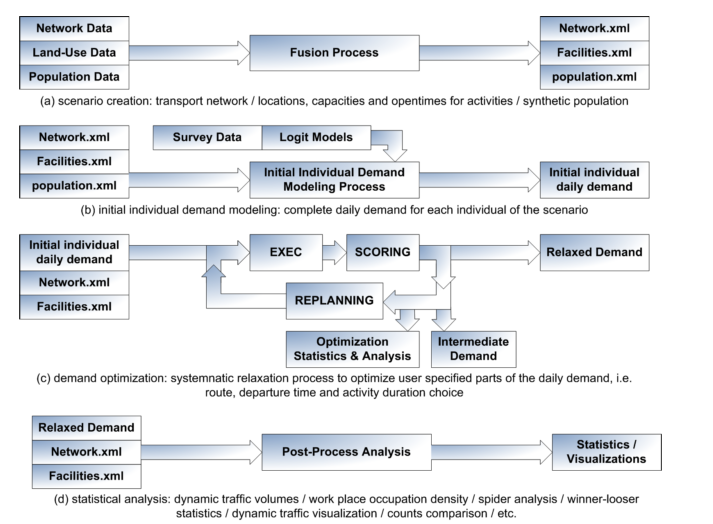
\includegraphics[width=14cm]{matsim-schema}}
\caption[MATSim schema (permission: Michael Balmer)]{Schema of the MATSim
model \citep{Balmer2009}. Thanks to Michael Balmer for permission.}
\label{fmatsim-schema}
\end{figure}

Because MATSim builds on Kai Nagel's experience as a computer scientist, who
also developed the highly successful TRANSIMS model (described below),
it has several advantages over competitors. These include:
\begin{itemize}
 \item ``MATSim is consistently constructed around the notion that travellers
 (and possibly other objects of the simulation, such as traffic lights) are `agents',
 which means that all information for the agent should always kept together in
 the simulation at one place'' \citep[p.~9]{Balmer2009}. This allows demographic
 data on each traveller to be instantly available, rather than being completely
 unavailable (as in most transport models),
 or available in a fractured file system (as in TRANSIMS).
 \item MATSim is fast to run in comparison with other transport
 models with similar specifications.
 \item Strong user community. As of May 2013, there is a comprehensive
 new tutorial on how to install and use MATSim (see
 \href{http://www.matsim.org/docs/tutorials/}{MATSim.org's tutorials site}),
 and daily commits to the source
 code (see \href{http://sourceforge.net/apps/trac/matsim/timeline}{sourceforge.net}).
\end{itemize}
For these reasons, and due to its accessibility to anyone with a modern computer,
MATSim has been identified as the most appropriate pre-existing model for
interacting with the data and methods presented in this thesis. MATSim
was carefully designed from the ground up to be the most powerful, user-friendly
and fast agent-based transport model available. It is important to recognise
that in order to avoid trying to `re-invent the
wheel'.\footnote{See \cref{s:workdes}
for a crude attempt to integrate the road network in the spatial microsimulation
--- a MATSim implementation may have been more appropriate given sufficient
time.
}
% Insert here an image of MATSim (Balmer2009) and where my model fits in 

\subsection{Land-use transport models}
% ``The first generation urban models were designed and implemented in
% North America mainly during the years 1959-68, years which coincided
% with the launching of large-scale land-use-transportation studies in major
% metropolitan areas.''
Researchers now have decades of experience modelling individual agents
\citep{Ortuzar1982},
transport flows \citep{Wilson1970} and the land-uses that lead personal
transit to take place \citep{batty1976urban}.
Of course, each of these elements depends to some extent on the others, so
integrated land-use transport models have long been regarded as the holy grail
in urban modelling. It is only recently that the computational
requirements of this task have been
available.\footnote{The memory requirements alone of storing a detailed
transport network in RAM are large. Combining this with complex polygons
defining administrative zones, a detailed microdataset and then performing
calculations defining how each model object changes from one moment to the next
in high temporal resolution is clearly a taxing computational task.
}
Despite the daunting complexity and data and computational requirements of such
models, their design and implementation has been theorised and attempted
since the 1960s, with limited levels of success
\citep{timmermans2003saga}. The author of this critical review went so far as
to suggest that the costs invested in ambitious land-use transport models
generally outweigh the benefits.
% ``There seems insufficient support for
% such investment, especially because the field has not succeeded
% in commercialising the short-term forecasts of traffic flows''
% \citep[p.~3]{timmermans2003saga}.
On the other hand, some have argued that it is only with modern computers and software
that integrated land-use transport models can move from a mere
`dream' \citep{timmermans2003saga}  into reality: ``recently,
the development of large-scale integrated land-use and
transportation microsimulation systems such as ILUTE ... ILUMASS
... and UrbanSim has generated a new excitement in the field'' \citep[p.~935]{Pinjari2011}.
These models, and TRANSIMS, are outlined below.

% A number of integrated models have been developed
% \emph{RAMBLAS}

\emph{ILUTE} \index{ILUTE} represents the `third wave' of transport-land use
models based on individual level data:
``[it] represents an experiment in the development of a
fully microsimulation modelling
framework for the comprehensive, integrated modelling of urban transportation-land use
interactions and, among other outputs, the environmental impacts of these interactions''
\citep[p.~15]{timmermans2003saga}. Thus ILUTE can be used to analyse a wide range
of phenomena: it is an integrated urban model in the fullest sense of the word
and has been even been used to analyse the distribution of house prices
in and large city over time \citep{Farooq2012-integreted}.

%\emph{TRESIS}
\emph{UrbanSim}, like ILUTE, is a micro level integrated land-use transport
model, aimed at \index{UrbanSim}
``incorporating the interactions between land use, transportation, the economy,
and the environment'' (\href{http://www.urbansim.org/Main/WebHome}{urbansim.org}, 2012).
The source code (written in Java and Python)
is open source and remains under continued development \citep{Nicolai2012-matsim}.
Perhaps because the software is free for anyone to download, use and modify,
it has been used for a range of applications including as a tool
to aid planners in the evaluation of transport projects \citep{Borning2008}.
Although UrbanSim does not contain an advanced transport module,
work has been done to integrate the dedicated transport MATSim model (see
\cref{s:dedicated}) into it,
via a plug-in \citep{Nicolai2012-matsim}.

\emph{TRANSIMS} \index{TRANSIMS} was developed at the Los Alamos National
Laboratory with an
ambitious objective mirroring that of ILUTE:
``to model all aspects of human behaviour related to
transport in one consistent simulation framework''
\citep[p.~1]{nagel1999transims}.  The model, which is based on cellular
automata, has been given a public licence (the NASA Open Source Agreement
Version 1.3), is cross-platform (with Windows and Linux binaries) and has been
widely adopted.\footnote{``TRANSIMS''
was cited 166 time in Google
Scholar in 2012 publications, many of which implemented the model for their own
applications.}
% It would be good to have ``n. times cited, 2012'' as a variable in comp. tab.
The encouragement of community contributions and an experienced development team
has led the model to be extended various ways. For example, TRANSIMS can be
configured to take advantage of parallel processing (in which one CPU is
allocated to each area being modelled) \citep{nagel2001parallel}, or external
programs for the visualisation of results
(http://sourceforge.net/projects/transimsstudio). The sub-modules of TRANSIMS
include a micro level population synthesizer, a trip generator, route planner
and microsimulator (which determines the location and behaviour of each
individual at each time step). The model is being increasingly adopted by
Municipal Planning Organizations (MPOs) in the USA \citep{lawe2009transims,
ullah2011travel} and has successfully simulated the entirety of Swiss travel
flows (around 10 million trips), using a `Beowulf cluster' of parallel computers
\citep{Raney2003}.

The modular design of TRANSIMS means it can be used in conjunction with the
spatial microsimulation methods presented in this paper. The small area
microdata could, when allocated home-work pairs, be used as an input forming
the baseline situation at time zero. The potential for combining the spatial
microsimulation methods presented in this thesis with additional modelling
tools is described in chapter 8.
% !!! Include this !!!

\section{Summary: research directions and applications}
\label{s:bigdata-gps}
Over time the uses of spatial microsimulation, in its broadest sense,
have expanded from a way of
providing quantitative geographers and others with individual level data, into a more
general modelling strategy harnessed to tackle many problems.
In this thesis, however, a narrower definition is used:
spatial microsimulation here refers to the process of generating spatial
microdata, analogous to `population synthesis' in transport models.
As in many fields, the
rate of change has also increased, due to increased availability of
sophisticated software, large datasets and powerful
computers. One could make the argument that the
uses of spatial microsimulation, as defined above, have become more specialised
as it is adopted by various fields for their own purposes, sometimes under
different names. This fragmentation is aggravated by the fact that
many do not make the code used for their analysis available, a
practice prevalent across the sciences \citep{Ince2012}.
However, there are also signs of integration. With the continued growth of
open source software and the greater dissemination of code
(e.g.~through sites such as Github), a kind of evolutionary process can be observed:
winners are picked and then generalised to be applied to a range of
problems.\footnote{A
good example of this positive-feedback process of picking winners, whereby
the most promising projects receive much new attention and then grow most
rapidly as a result (of peer feedback and new collaborators), is MATSim.
Released as an open source project in 2006, the project has rapidly gained
users, contributors and policy applications. MATSim also illustrates the
wide appeal of microsimulation software, finding applications as ranging from
a `plugin' to pre-existing urban simulation models to a framework for
modelling leisure and shopping trips \citep{Nicolai2012-matsim, horni2009location}.
}
% \citep{Clarke2013-concs}

The rate of change is fast, yet it is important to make use of more than 30 years
. Looking back, it is possible to reflect
on what works and what does not work so well in spatial microsimulation
research. Summarising a large body of experience,
\citet[p.~197]{Holm2013-design-principles} created the following `wish list' of
factors that future spatial microsimulation researchers should consider
when creating new, or updating existing, models:
\begin{itemize}
\item  use the most modern software
\item  use standard methods, shared by many users
\item  backward compatibility (so keeping our old models and subsystems running)
\item  avoid relearning
\item  develop solutions that are theoretically well designed
\item  transfer knowledge and know-how to new colleagues
\end{itemize}
It is interesting to note that this list could have been as applicable 30 years
ago as it is now, indicating key areas of continuity in the field.
Effort has been invested throughout to comply with these
principles. It is hoped that the focus on the final point, dissemination of methods,
will enable spatial microsimulation to be used by policy
makers.\footnote{To
this end, experiments to improve the performance of IPF and some other
script files that may be of use to others
have been put online via the dissemination portals www.rpubs.com/robinlovelace
and www.github.com/robinlovelace . Knowledge transfer was also behind the
publication of a user manual alongside \citet{Lovelace2013-trs}.
}
Indeed,
its potential for policy evaluation, at individual and local levels, was
one of the major reasons for choosing the spatial microsimulation approach
to tackle the problem, helping to fill the `scale gap' between academic
studies and policy interventions described in \cref{Chapter2}.

The literature summarised in this chapter should make it clear that
the methods used are not new: researchers have been modelling
transport problems at the individual level over two decades \citep{Ortuzar1982},
and developing the theory behind individual level behaviour for even longer
\citep{Wilson1970}.
The novel
contribution made in this thesis is the practical \emph{application} of
the existing method of spatial microsimulation to the problem of unsustainable
commuting. Approaching the issue from a quantitative geography and spatial
microsimulation perspective allows the focus on spatial
variability and social inequalities in transport energy use, highlighted in
\cref{Chapter6} to \cref{Chapter8} of this thesis. This is in contrast to the 
transport modelling perspective, which is still largely traffic-orientated.
Before proceeding to apply
the method, however, it is vital to understand precisely how the
spatial microsimulation model used in this thesis works and the input data.
That is the task of the next chapter.



%!!! include these!!!
% \subsection{`Big data'}
% \subsection{GPS-loan surveys}
% \subsection{Applications for model validation and enhancement}
\label{s:applications}

%%%%%%%%%%%%%%%%%%%%%%%%%%%%%% Deshets
% In economics, spatial microsimulation has been used to \citep{Cullinan2011}
 % Msim introduction

% Chapter 4: coming along nicely. Be concise

\chapter{Data and methods} % Write in your own chapter title
\label{Chapter4}
% \lhead{Chapter 4. \emph{Data and methods}} % Write in your own chapter title
\fancyhead[RO,LE]{Chapter 4. Data and methods} %2side
\fancyhead[RE,LO]{\thepage}
\section{Introduction} 
% this thesis is a data-driven exploration of the energy costs of commuting.
To fully describe and understand the energy used in travel to work, a large
amount of data is needed. Behavioural, technical, infrastructural and even
economic data would be required at a high level of spatial and temporal
resolution over a wide area and a long timespan to provide a complete
picture of the flows within the transport-to-work energy system. %!!! Make this
The ideal dataset would also contain grid references of both the origin and
destination of every trip to and from work, the
route distance (which may change from one day to the next), the specifications
of the primary vehicle used and, ideally, measurement of the food or fuel
consumed as a result.

It is worth briefly considering what this giant dataset would look like: the
methods can be seen as an attempt to approximate a simplified version this
omniscient information source, through modelling. \Cref{fdata-ideal} illustrates
the numerous connections to additional datasets not traditionally included in
travel surveys that would be needed for the most detailed view.
The thought experiment led to the imaginary Comprehensive
Commuting-Energy Database (CCED). This main dataset would be part of a wider
`data schema' of connected tables \citep{Obe2011} as it would depend on
detailed additional
information about individuals, the vehicles they drive, up-to-date
information on where they live and work, as well as detailed information on
every single trip to work they make for an accurate assessment of energy costs
and the factors influencing them. To gain an understanding of the complexity of
this dataset, let us picture its size for the UK. Assume that 30 million people
are employed,\footnote{During
the 3$^{rd}$ quarter of 2012, there were 29.86 million
employed
people in the UK according to the
\href{http://www.ons.gov.uk/ons/dcp171778_292911.pdf}{Office for National
Statistics}}
making, on average, 200
home-work round trips per year. This would mean the CCED would need to contain
12 billion rows of data each year. Even ignoring the complexities added by the
linked datasets,\footnote{The CCED would need to link to the constantly changing
home-work
locations (currently untracked by the government, except during the census),
household composition, energy use data and vehicle ownership datasets. This
would require constant, probably automated monitoring and computer
infrastructure that is currently beyond most local authorities to store, analyse
and interpret. Large data management
organisations such as Google and Facebook have shown that such vast
`live' databases are possible, however. A state-controlled online
data-logging system, which harnesses near-total smart-phone penetration, could
conceivably move towards this vision. } keeping this dataset updated live would
be far beyond the government's current official data collection capabilities.
The largest microsimulation run performed for this research was of $\sim$2 million
commuters in Yorkshire and the Humber, over 3 orders of magnitude smaller that
the CCED for a single year. Given that the analysis was unwieldy, it seems such
a large dataset would pose major problems to current mainstream computer
hardware.

\begin{figure}
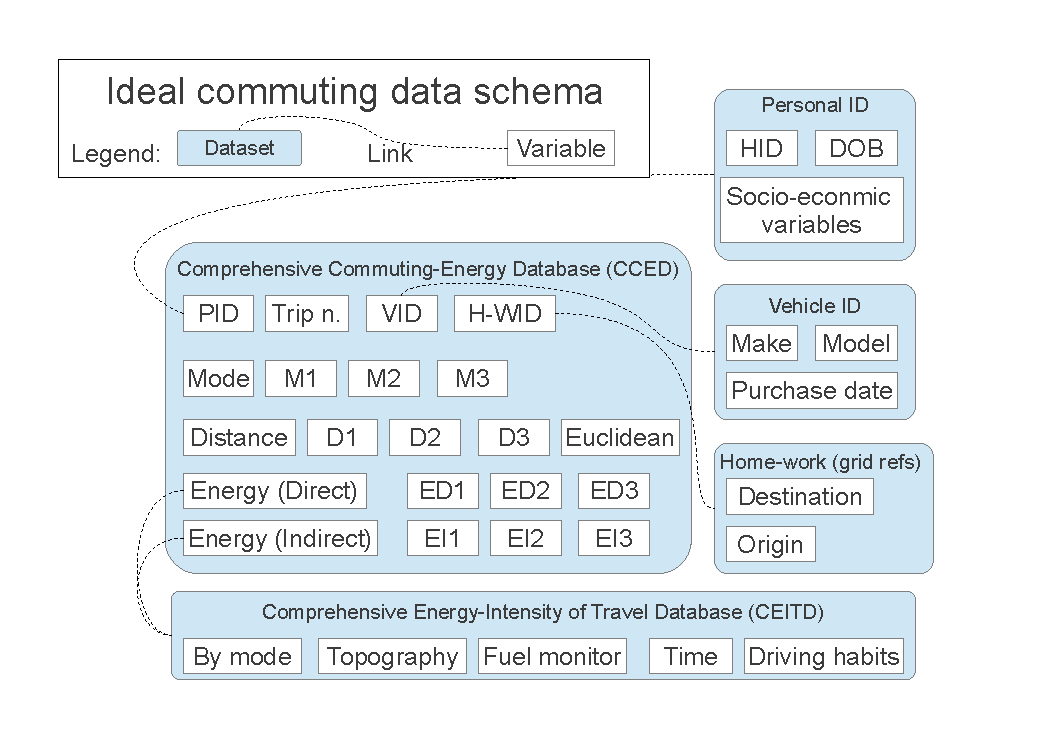
\includegraphics[width=14cm]{data-ideal}
\caption[Idealised data schema for studying energy use in commuting]{Idealised
data schema for studying energy use in commuting. The imaginary CCED database
would need to link to other, equally detailed datasets to work.}
\label{fdata-ideal}
\end{figure}

Of course, the available datasets do not match the detail of the imaginary CCED.
Budgets for data collection, confidentiality and technical
considerations combine with the practical
difficulties of monitoring the energy used by hundreds of thousands of unique
vehicles. Based on these difficulties, one could argue that the data
limitations are insurmountable and that more qualitative approaches are needed.
This research is based on the opposite view: that the inherent data limitations
mean that the datasets that \emph{are} available are
absolutely critical. Systematically collected data has a much better chance of
meeting the research aims, as set-out in \cref{s:aims} than purely qualitative
information. Without good statistics, one would have to resort to personal
observation and anecdote, sources that are unlikely to be
representative of the system as a whole \citep{Rubin1987}. Because the available
datasets cannot be
changed, whereas the methods used to analyse and model them can, the approach
taken here is \emph{data-driven} (as opposed to model driven)
\citep{anselin1989special}: the starting-point is the available data.
After the introduction, this chapter describes the input
datasets (\cref{senergyusedata} to \cref{sadditional}) and then
explains the methods used to process them and evaluate the outputs (\cref{setsim} to
\cref{smeval}). The final section explores methods for generating
integer results, which are useful in agent-based applications (\cref{s:integerisation}).

Due to its policy relevance, the methods 
are treated primarily as means rather than ends in themselves throughout
the majority of the thesis. In this chapter the emphasis reverses, and the methods
(and the datasets on which they depend) become the focus. It would be an
exaggeration to say that the data and
methods are seen here as ends in themselves, as they all contribute towards the
aims. Yet effort has been made to explain them in general terms. An
additional aim of this chapter is to illustrate clearly how the methods
were implemented, allowing others to replicate the results. It should also be
clear by the end of this chapter that the methods could be harnessed for
purposes other than assessment
of the energy costs of travel to work. They could be used
for a more conventional economic evaluation of work travel, as the basis of
agent-based models of employee behaviour (see
\cref{s:integerisation} on integerisation) or for the analysis
of individual level processes based on aggregate data more generally.

As discussed in \cref{Chapter3}, reproducibility of methods is one of the
cornerstones
of scientific advancement yet it is often missing in spatial microsimulation and
related fields. Therefore, this an important chapter from an academic perspective:
it allows others build on the analysis, by applying the methods to new datasets
and extending or modifying the methods for their own purposes. 
There have been some methodological advancements ---
such as a new algorithm for the integerisation of IPF weights and
the allocation of origin-destination co-ordinates to individuals
simulated using spatial
microsimulation.\footnote{Individuals
have been allocated locations and other characteristics in
existing micro level transport models such as
MATSim (\cref{Chapter3}). However, these models focus on transport:
individual level attributes provide an optional add-on.
The methods presented in this thesis operate the other
way around: micro level characteristics generated by spatial microsimulation
form the foundation; transport patterns are the add-on.
}
% and development of flow mapping visualisations using the R package
% ggplot2. %!!! add this back in when flow mapping section is included
However, much of the work simply applies existing methods in a
new context.

The advantages of spatial microsimulation over purely aggregate or
individual level analyses are described in general terms in the previous
chapter. The reasons behind the choice of spatial
microsimulation for this particular application relate to the available
datasets, and should become clearer as they are described. Essentially, there is
no single, comprehensive dataset on travel to work patterns in the UK and its
energy implications, such as the imaginary CCED described above. Various
datasets are available, each with its own
advantages and disadvantages. Spatial microsimulation can be used to combine the
main
official and un-official sources of data, and provide individuals whose travel
patterns can be modelled. The main datasets used in this thesis are:
\begin{itemize}
 \item transport energy use data % Yes
 \item the 2001 Census of UK population % Yes - not all working... - should add other censuses!
 \item the Understanding Society dataset (USd) % Check: UKDA2
 \item the 2002-2008 National Travel Survey (NTS) % Yes - data large
 \item transport infrastructure from Open Street Map (OSM) and
other sources % Yes - not local though
\end{itemize}
The first data source to be described is on direct energy use in transport,
in \cref{senergyusedata}, as good energy data are vital to
the results chapters. Although energy use can be calculated based on
mode, distance and other variables, this official source provides energy
data directly. Because of the limitations of these official energy use data
(in terms of coverage of modes, lack of disaggregation by reason for trip
and course geographical resolution), good data on commuting
\emph{behaviour} are needed to calculate energy costs indirectly.
This information is reported in \cref{ssocialsurveydata}.
Social survey data are made available both as geographically aggregated
counts from the census (\cref{sgeoaggdata}) and more detailed individual level
variables from  nationwide surveys which take a representative sample of
the UK population (\cref{sUSD} and \cref{snts}). The final type of data
considered
provides geographical context --- the location of roads, railways and other
infrastructures, as well as information about elevation and other
geographical variables. These datasets are described in \cref{sadditional}.

Each data source has advantages and disadvantages.
The census dataset is the most geographically comprehensive 
(covering virtually every commuter in the country) but is limited in terms of
the number of variables on offer (mode and linear distance of home-work
travel) and the fact that it is geographically aggregated count data, providing
little sense of individual level variation. This can be supplemented by datasets
that operate at household, individual and (in the NTS) trip, stage and
vehicle levels. The Understanding Society dataset (USd) is a general purpose
national survey, so it has a wide range of socio-economic and attitudinal variables
that are useful in explaining observed commuter patterns. It is also
longitudinal, and provides some information on car ownership, so could be
useful for assessing how commuting patterns evolve over time and relate to car
ownership at the individual
level. The National Travel Survey (NTS) is the other individual level dataset
used. It is
much more focussed on transport and
provides detailed information on trip distance, duration, mode and the
reasons behind travel. Because this dataset is based on
week-long travel diaries, and provides information collected over all seasons
over the course of 7 years, it allows assessment of commuter habits over time,
on weekly, seasonal and inter-annual time-scales. Additional datasets are
geographical, with accurate co-ordinates allocated to physical features and
elements in the transport network. Including these
in the analysis is challenging, but provides useful insight into the possible
underlying environmental reasons behind variation in commuting habits.

\section{Energy use data} \label{senergyusedata}
Energy use in transport is, in
general, uncertain, due to the various system boundaries, conflicting sources
and multiple definitions of what actually comprises energy (e.g.~the distinction
between direct and indirect energy use). Official data on the subject therefore
provides a useful benchmark against which calculations of energy use can be
compared.
(Estimates of energy use by mode, as opposed to
the official datasets presented in this chapter, are described and discussed in
detail in \cref{Chapter5}.) %!!! Opportunity for validation!
The uncertainty arises because
energy costs of personal travel and hence commuting are not recorded in
the same way as
household energy use (available at MSOA level from Neighbourhood Statistics) or
sub-regional fuel statistics \citep{Decc2008}. Cars, for example,
are mobile energy users that
can refuel anywhere, so tracking their use of fuel is not currently
feasible.\footnote{This
has the potential to change with the emergence of
in-car fuel use monitoring. Technologies range from the simple and cheap
(FuelLog is a smartphone app which costs under $\pounds2$) to the expensive
and complex (e.g. Scanguage --- a retrofitted fuel monitor).
Some models now come with fuel efficiency monitors pre-installed
(e.g. all Nissan Micra models, since 2007). Despite these advancements
and the acknowledged important of fuel consumption Department for Transport
currently has no plans to record fuel use alongside other data such as
odometer readings which are routinely taken during the MOT (Rachel Moyce,
DfT employee, personal communication).
}
Similar
problems exist for public transport, where officially reported aggregate values
are often the only source of data (see \citealp{LondonUnderground2007}).
Worse, the estimated energy costs of walking and cycling  vary widely from study
to study and are subject to a high level of uncertainty
\citep{Coley2002, Brand2006, Lovelace2011-assessing}.

As indicated in \cref{Chapter1}, %???,
the energy costs of commuting have not been previously analysed in detail.
There is little direct evidence about the energy costs of transport to
work, let alone its geographic variation: fuel use can be estimated for
motorised transport vehicles, but regional statistics do not provide break-downs
by trip reason, distance, socio-demographic category or low (sub Local
Authority) levels geographic aggregation. One dataset \citep{Decc2008-tcons,
Decc2013-regcons} does
provide direct estimates of transport energy use (\cref{t:deccdata}).
% Due primarily to the lack of
% dis-aggregation the available data do not provide an
% adequate basis for decision makers tasked with getting people to work more
% sustainably.
% The subsequent chapters therefore describe how energy use of
% commuter transport systems can be calculated, and explain the factors that lead
% to uncertainty and variability in these estimates. For now, we present the
% official data that is available.

\begin{table}[h]
\centerline{}
\caption[Sample of regional transport energy consumption statistics]
{Sample of the regional transport energy consumption statistics released by
\citet{Decc2013-regcons}. 2010 data shown: available each year from 2002.}
\begin{tabular}{llrrrr}
\toprule
\multicolumn{1}{c}{} & \multicolumn{1}{c}{} & \multicolumn{ 4}{c}{Energy consumption (Thousand tons of fuel)} \\
\cmidrule{3-6}
\multicolumn{1}{c}{LAU1 Code} & \multicolumn{1}{c}{LAU1 Area} & \multicolumn{1}{c}{Buses} & \multicolumn{1}{c}{Diesel Cars} & \multicolumn{1}{c}{Petrol Cars} & \multicolumn{1}{c}{Motor-cycles} \\
\midrule
UKL1605 & Blaenau Gwent & 0.9 & 5.6 & 9 & 0.1 \\
UKL1705 & Bridgend & 3.1 & 21.2 & 30.6 & 0.3 \\
UKL1604 & Caerphilly & 3.2 & 18 & 28.8 & 0.3 \\
UKL2207 & Cardiff & 8.3 & 48.8 & 75.1 & 0.6 \\
% Could you not include another line: uk total???!!!
\bottomrule
\end{tabular}
\label{t:deccdata}
\end{table}

The data presented in \cref{t:deccdata} is useful for providing an overall
picture of the spatial variability of energy use within the UK. (The units are
easily converted into Joules, the energy unit used here using the
following conversion factor: $1~Toe = 42~GJ$ or $1~MToe = 42~PJ$). The dataset
also includes estimates of the energy consumption by light and heavy goods
vehicles (LGVs and HGVs respectively). This allows for personal travel to be
placed in the wider context of overall travel: energy use for freight is just over
half (55\%) that of energy used for personal travel modes. This shows that
energy in transport
studies should not be limited to personal travel alone; moving goods
uses over a third of the total energy use (35.3 $GToe$). In addition to these
benefits, the data are temporal: it would allow changes in the geographical
distribution of energy use in transport overall to be compared with shifting
patterns of energy use for travel to work estimated from census data.

The data does have limitations, however. First, there is no breakdown of the
data by reason for trip, so the fuel consumed by travel to work (as opposed to
other types of trips such as leisure) must be estimated as a proportion of the
total. A simple way of doing this is to simply multiply all fuel use values
by 0.195, the proportion of total passenger kilometres attributable to
commuting \citep{NationalTravelStatistics2012}.\footnote{Commuting is jointly
the greatest reason for person-kilometres in the UK (to the nearest percentage
point) along with ``visiting a friend'' (19.7 \%) and ``other leisure'' (20.4
\%). This dataset is from 2010 and can be found in Table NTS0402 from
\citet{NationalTravelStatistics2012}.
}
The most obvious problem with this approach is that the proportion of
distance travelled by each reason for trip varies greatly from place to
place, %!!! by how much? Write this up at the LA level.
so such a crude estimate will be highly innacurate. More sophisticated
methods of translating the total into commuter energy use only could be used,
but these rely on datasets from which energy use estimates can be produced
directly anyway. Therefore the main strength of the dataset is that allows
commuter energy use to be compared with total energy use for personal travel at
the LA level.%!!! where???

Another problem with the \citet{Decc2008-tcons} dataset is that it includes only
road-based traffic. Walking, cycling, trains, trams and the underground, which
make up almost 1/4 of trips to work in the UK, are
omitted from the analysis. This is especially problematic for use of the
dataset in what-if scenarios, as these are precisely the modes that would
need to grow fastest in a low energy future. In terms of distance travelled,
the omission could be justified as the three main road-based modes (car
drivers, car
passengers and bus) accounted for 84\% of passenger kilometres in 2010
\citep{NationalTravelStatistics2012}. In terms of energy use, non-road modes
are even less important, as they consume a fraction (specifically, less than
one twentieth) of the energy per unit
distance than cars and buses. The final problem with the dataset is its coarse
geography: it would be of little use for local decision making processes. This
coarseness is put in perspective \cref{t:agdata} and \cref{f:scales} below.
 
% \section{Commuting data}
\section{Social survey data}
\label{ssocialsurveydata}
The best source of commuting data in terms of coverage in the UK
is the national census, which must be answered by every household. The dataset is
released a year or so after
each census, which has taken place every 10 years (except 1941)
since 1801. Dating back to at least 1971 (the earliest date for which travel to
work data are available via the census data dissemination portal Casweb), there
has been a question on mode of travel to work \cref{fq33} (left).
This dataset is provided for a 10\% sample before 2001, which is
problematic in small areas.\footnote{The dataset is provided down to enumeration
district (ED) level, each of which contained $\sim$500 residents since 1971, and
down to the output area level ($\sim$300 residents) since 2001.} Since 2001,
the data has also provided breakdowns of travel to work by distance, crucial to
constraining estimates of energy use for travel to work. (Distance is not
reported directly by respondents, but calculated as the Euclidean distance
between the area centroids of home and work postcodes --- see \cref{fq33}
(right).) For all time periods, the data can be cross-tabulated by social class.
This is important for understanding how commuting energy costs vary across
social class and the likely distributional impacts of change. 

\begin{figure}[h]
 \centering
 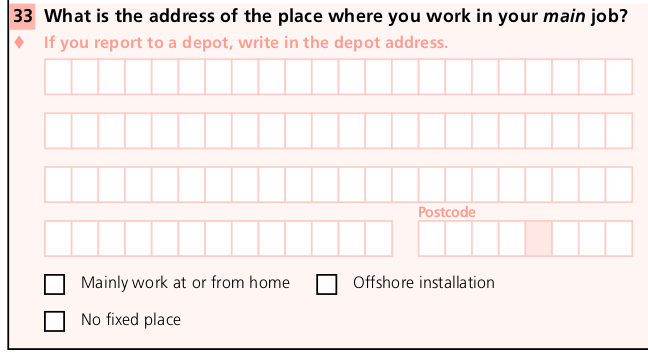
\includegraphics[height=5cm]{q33}
 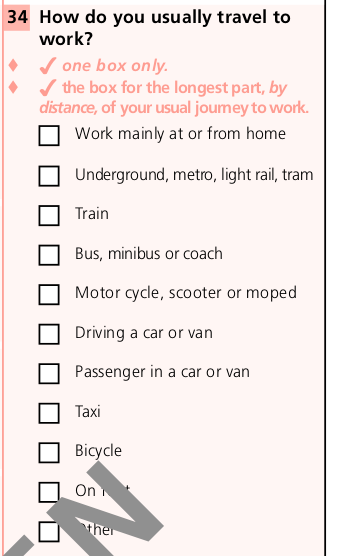
\includegraphics[height=7cm]{q34}
 % cc-trans.png: 1113x529 pixel, 72dpi, 39.26x18.66 cm, bb=0 0 1113 529
 \caption[Questions 33 and 34 of the 2001 UK Census]{Questions 33 and 34 of the
2001 UK Census, which provide information
on mode (left) and distance (right) travelled to work, respectively.}
 \label{fq33}
\end{figure}

These data are available at the individual level through the Sample of
Anonymised Records (SARs) for 1 and 2\% samples of the entire survey.
For the purposes of this study, however, alternative sources of individual
level commuting data were used, to provide additional variables. The main
use of census data, therefore, was as a source of `small area constraints'
(described in \cref{s:defs})
for spatial microsimulation, at various levels of geographic aggregation. 
The main disadvantage of the census
dataset is that it only provides information about a small number of variables
compared with more specific surveys that have lower samples sizes. Only 57
questions were asked in the 2011 Census. By contrast, the number of variables
in the NTS and the USd datasets runs into several hundred.

\subsection{Geographically aggregated data} %Add what's available from 2011!!!
\label{sgeoaggdata}
Census data on commuting is disseminated by Casweb at a range of geographic
scales (\cref{f:scales}) and with a variety of cross-tabulations. Before
forging ahead and describing how the datasets are used, it is worth taking stock
of the scales of geographical aggregation at which they are available.
Consideration of the range
of options at the outset is especially important because research
findings can depend on the size and shapes of geographic zones,
the `areal units' of analysis \citep{Horner2002, Openshaw1983}. Selecting zones
that are too small relative to the study \index{scale} \index{geographic
aggregation}
area can lead to long processing times, messy maps and over-complexity.
Analyses based on overly large zones, on the other hand, can gloss over
spatial variability by presenting space in extensive, homogeneous blocks.
Regardless of the scale of analysis selected, it is important to remember that
\emph{all} analysis based on geographically aggregated data may be susceptible
to the modifiable areal unit problem (MAUP) \citep{Wong2009}.
% {\color{red} (Previous
% paragraph about MAUP deleted --- Robin)}

\begin{figure}
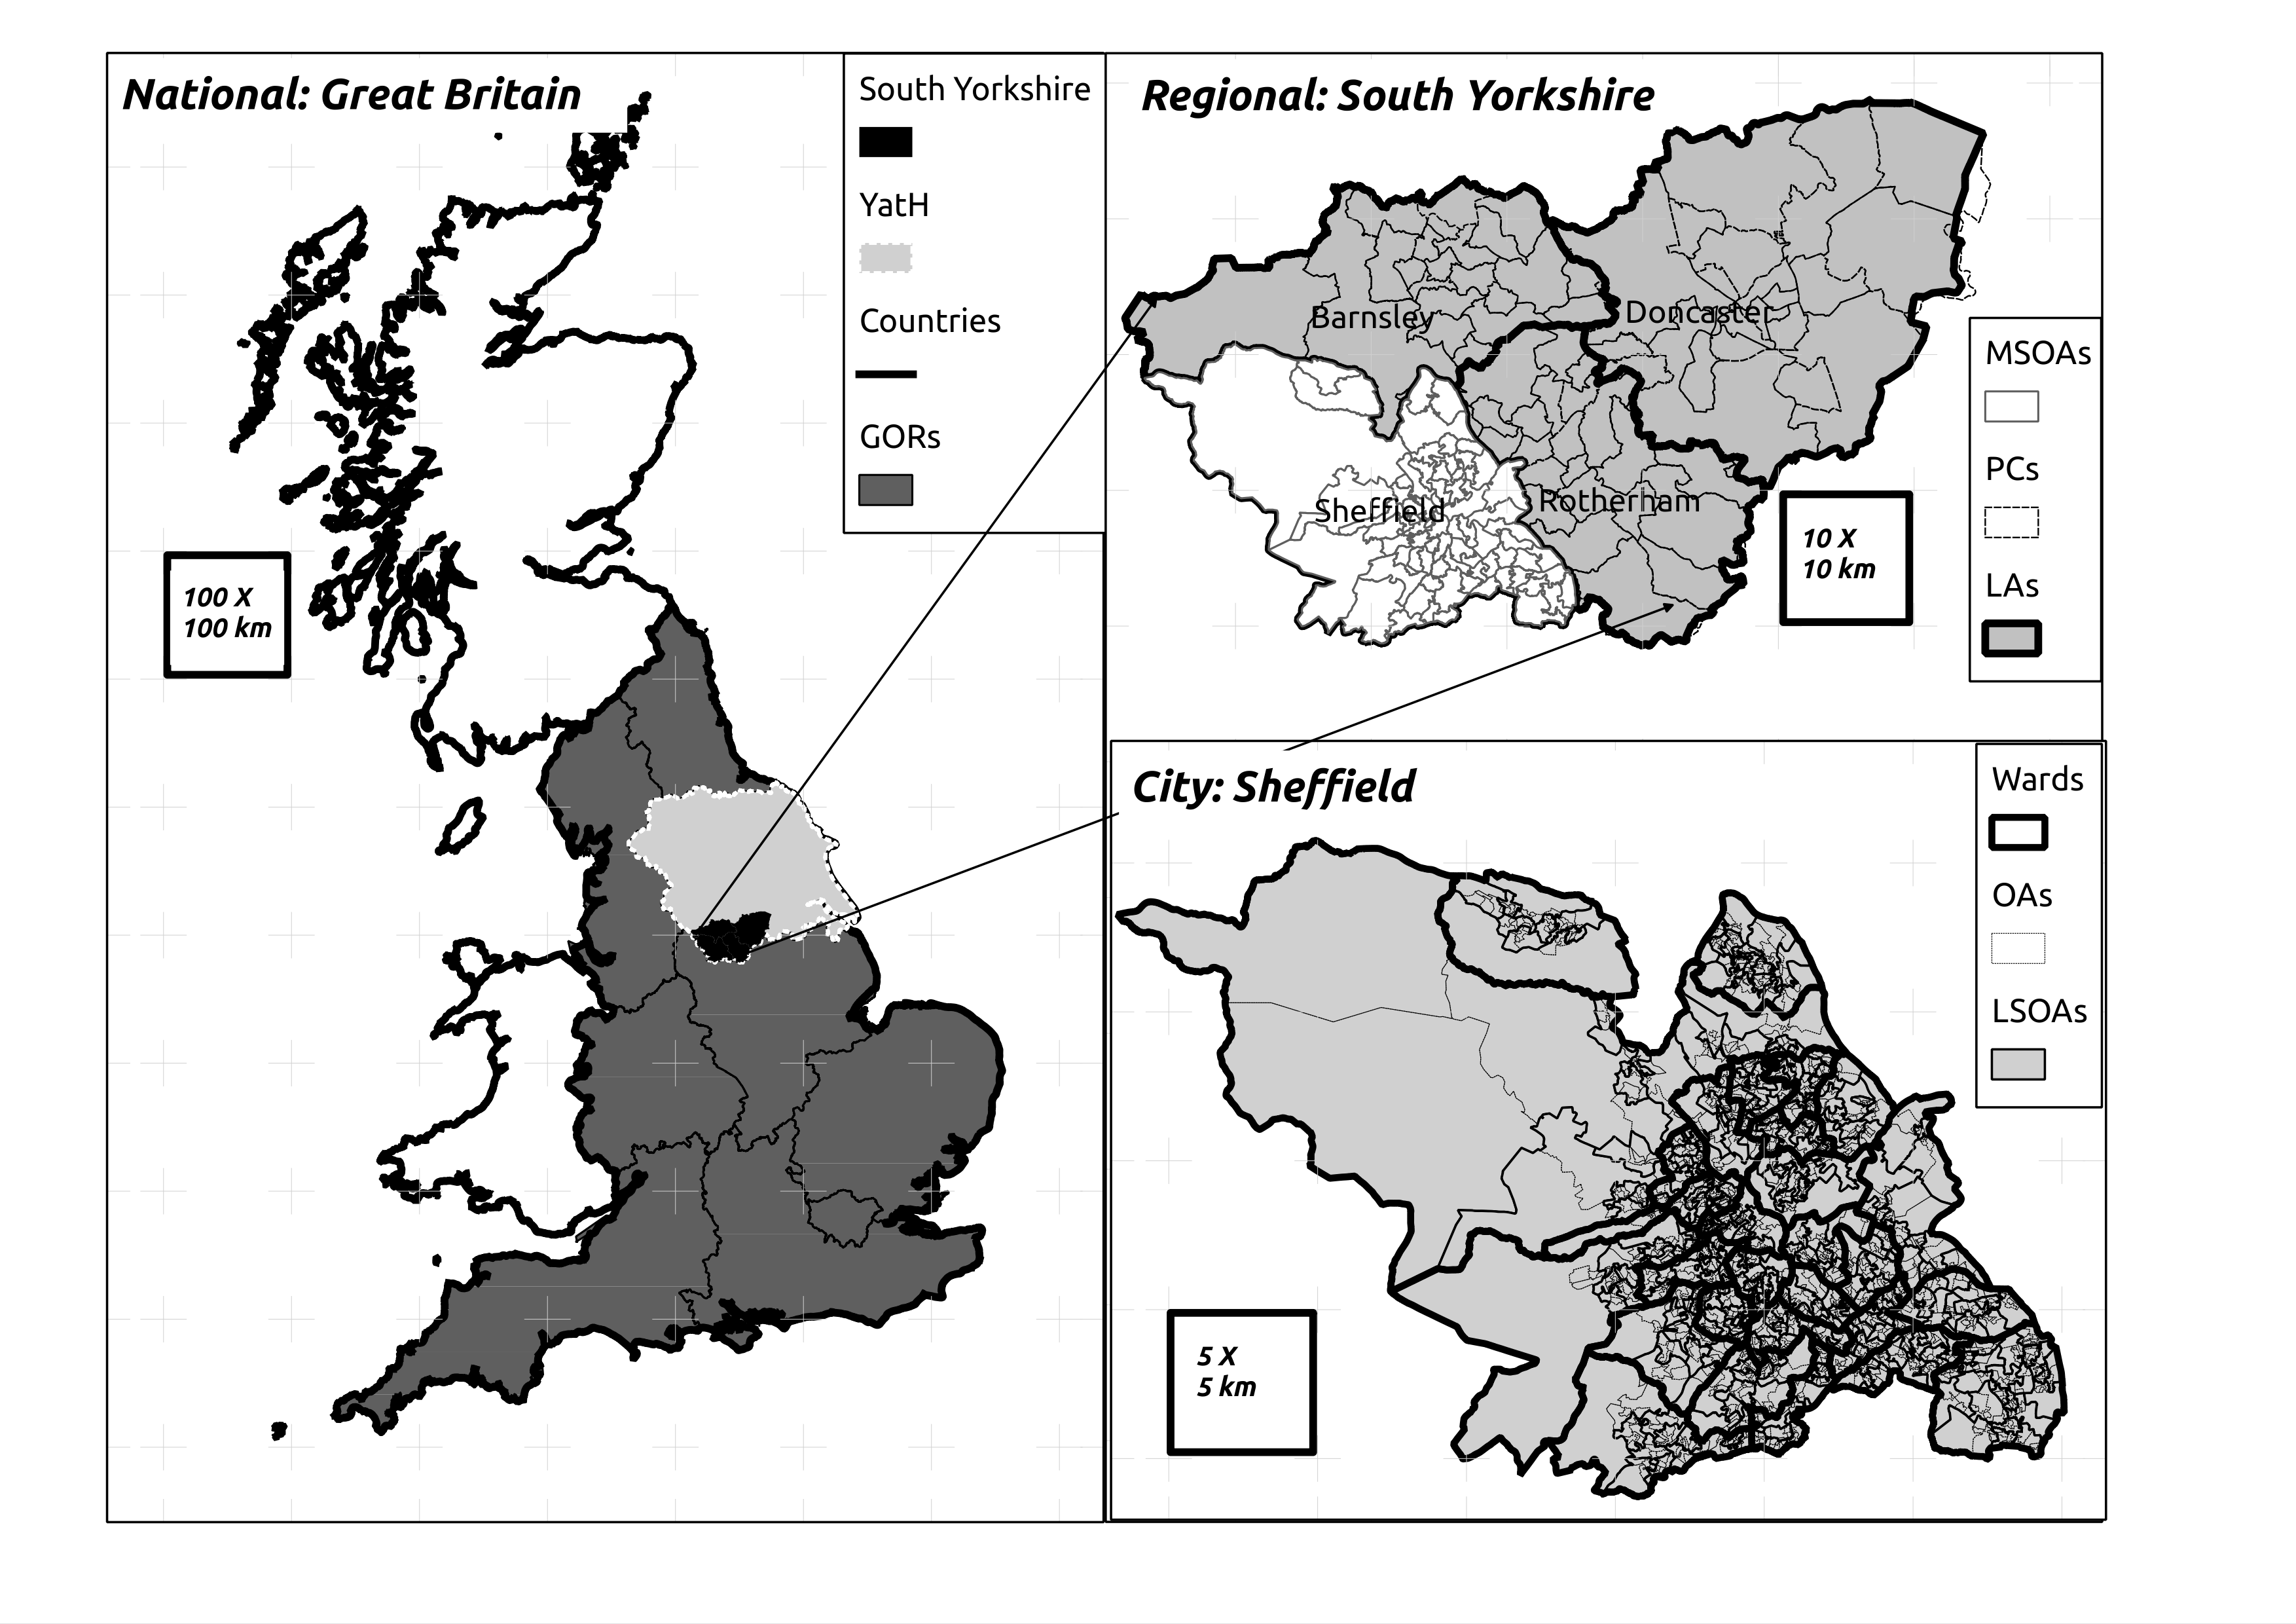
\includegraphics[width=14cm]{scales-map}
\caption[National, regional and city-wide scales of analysis]{National, regional
and city-wide scales of analysis, as illustrated
by a range of administrative boundaries. Yorkshire and the Humber (left),
South Yorkshire (top right) and Sheffield (bottom right)
are the study areas used for this section.}
\label{f:scales}
\end{figure}

% Understanding of the potential impacts of the
% MAUP, and methods for dealing with the problem have improved greatly since the
% 1980s \citep{Sui1999}. However, many studies within
% transport geography continue to follow the tendency of human geographers to
% ``opt for one level of analysis exclusively, without considering the range of
% alternatives'' \citep{Watson1978}. Geographical research on commuting is no
% exception \citep{Horner2002, Li2012}, tending to use only ``a single
% set of analytical [areal] units'' for each case study \citet[p.~40]{Sui1999}.
One of the advantages of spatial microsimulation is that it facilitates
`frame-independent' (scale independent) analysis \citep{Horner2002}. The
results for any particular region --- a table of geo-located individuals equal
in population to the commuting population of the region --- should be roughly
the same in terms of the size of the output file and distributions of
individual level variables, regardless of the scale of analysis. It is
still important to choose an appropriate scale, as lower
geographies will provide more localised information, yet be harder
to analyse and visualise. 
Spatial datasets related to commuting in the UK, and their scales of
dissemination, are outlined
in Table \ref{t:agdata}.\footnote{The administrative acronyms OA, LSOA,
MSOA, and LA refer to Output Areas (which contain $\sim$300 people),
Lower Super Output Areas ($\sim$1600 people), Medium Super Output Ares
($\sim$7000 people) and Local Authorities (more than 100,000 people)
respectively.}

\begin{table}[htbp]
\begin{threeparttable}
\caption[Aggregate data on energy costs of commuting by
scale]{Aggregate data related to the energy costs of transport to
work and the scales at which they are available for South
Yorkshire. The slash symbol (e.g.~in ``Mode/distance'')
represents cross-tabulation. Source: Casweb, unless otherwise stated.}

\begin{tabular}{|l|l|l|l|l|l|}
\hline
Variable & OA & LSOA & MSOA & ST Ward & LA \\ \hline
N. zones in South Yorkshire & \multicolumn{1}{r|}{4278} &
\multicolumn{1}{r|}{845} &
\multicolumn{1}{r|}{173} & \multicolumn{1}{r|}{59} & \multicolumn{1}{r|}{4} \\

Average population & \multicolumn{1}{r|}{296} & \multicolumn{1}{r|}{1450} &
\multicolumn{1}{r|}{7320} & \multicolumn{1}{r|}{21500} &
\multicolumn{1}{r|}{317000} \\
Mode of transport to work & Y\tnote{a} & Y & Y & Y & Y \\
Average distance & N & Y & Y & Y & Y \\
Distance categories & Y\tnote{a} & Y \tnote{c} & Y\tnote{c} & Y & Y \\
Mode/Distance & N & N & N & Y & Y \\
Car access\tnote{b} & Y & Y & Y & Y & Y \\
Domestic energy use\tnote{d} & N & N & Y & N & Y \\
Transport energy use\tnote{d} & N & N & N & N & Y \\
Total energy use\tnote{d} & N & N & N & N & Y \\ \hline
\end{tabular}
\begin{tablenotes}
\begin{footnotesize}
 \item [a] Output area statistics are often unreliable because values less than
3 are randomly allocated the value of 0 or 3. This is problematic for sparsely
populated categories such as those who travel 60 km or more to work.
\item [b] `Car access' refers to the census dataset `cars or vans' which
provides counts for the number of houses with access to no cars, one car etc,
and total number of cars in each area. This is for estimating reliance on
public transport.
\item [c] Data provide by Nomis government data portal, providing various
cross-tabulation options (\url{https://www.nomisweb.co.uk/Default.asp}).
\item [d] Data provided by the Department of Energy and Climate Change (DECC,
from
\url{http://www.decc.gov.uk/en/content/cms/statistics/energy_stats/regional/}).
\end{footnotesize}
\end{tablenotes}
\label{t:agdata}
\end{threeparttable}
\end{table}

As well as being available at different administrative geographies, the datasets
presented in Table \ref{t:agdata} are variable in terms of reliability, their
origin, and times of collection.
Following the `confidentiality principle' of
census data release \citep{Rees2002}, small numbers (3 or below) are allocated
as either 0 or 3 for census data.
This makes cross-tabulated datasets of unusual categories such as `cycles to
work' unreliable at the smallest Output Areas (OA) level.
Census data are the `gold standard' in terms of accuracy
and geographical coverage \citep[p.~4]{Martin2002}.
% : completion rates
% and levels of truth-telling are high for census surveys
% and its completion is a legal obligation for every UK citizen
% .
However, as mentioned earlier, the census lacks details covered by more
specific surveys. Of relevance to energy use, there is no information about the
type of car that car commuters used, or the route distance to work each of
which can have a large impact on overall energy use. The fact that census datasets
are only released every 10 years is a major disadvantage for dynamic analyses
compared with rolling surveys such as the NTS and the USd. It should be noted
that while the data provided by Casweb and Nomis are essentially the same,
% originating from analyses of census data,
the DECC data on energy use was collected in a different way and at a different
time, running from 2005 to 2010, as opposed to 2001.

\emph{Cross-tabulated counts}

Cross-tabulated count data refers to categories which are split up into
subsections. The cross-tabulation mode/distance, for example would contain the
number of car drivers who travel 0-2 km to work, 2-5 km etc.~and the same
sub-categories for every mode of transport. The number of variables (and hence
cells) multiplies with each additional cross-tabulation. To provide another
example, CAS119 (from Nomis) presents mode of travel to work (car, bus etc.) as
cross-tabulated by two other variables --- age and sex.
This provides the potential for more accurate microsimulation (by constraining
by more, cross-tabulated, variables) and a foundation for
validation. Disadvantages of Nomis include the increased likelihood of
empty cells in cross-tabulated data
% % Could mention here that Nomis data is randomised to protect anonymity
% However, priority now is to keep it short and sweet.
and `information overload' for the researcher: it is difficult to analyse and
visualise a 3 way cross-tabulated dataset including more than 100 variables,
such as CAS119, using standard methods of spatial data analysis.

\begin{figure}
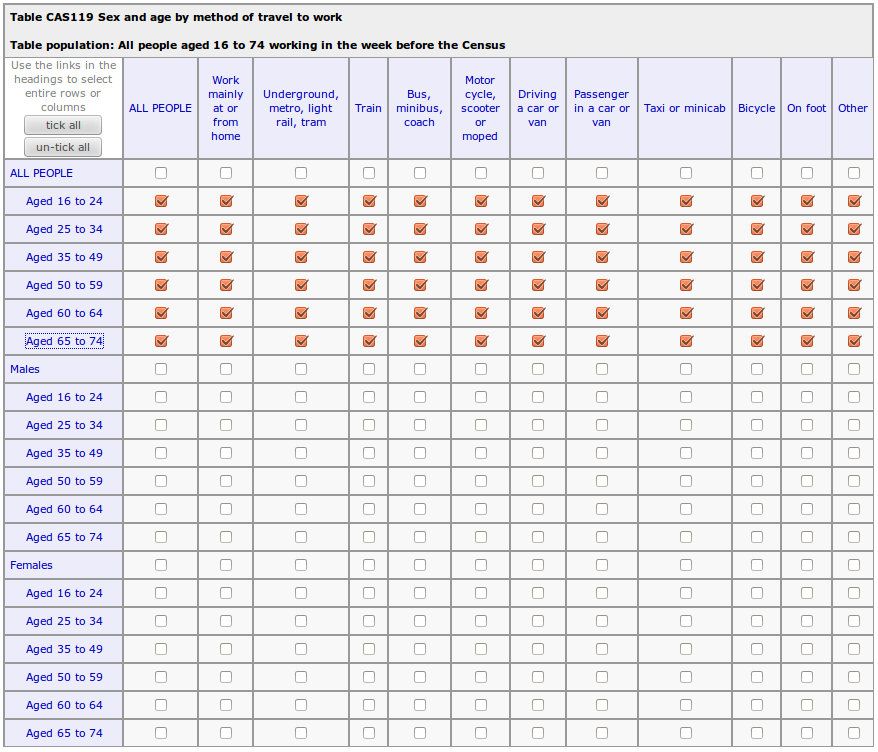
\includegraphics[width=13cm]{cas119}
\caption[Cross-tabulated dataset containing mode/age/sex
variables]{Cross-tabulated dataset containing mode/age/sex variables from Nomis
(dataset CAS119).}
\label{fig:cas119}
\end{figure}
Data size can be a problem: the selected variables presented in
Fig.~\ref{fig:cas119} represent 308,016 cells at the output area for
South Yorkshire\footnote{6 age categories multiplied by 12 mode
categories multiplied by 4,278 output areas.}
and takes up almost a megabyte of
hard-disk space just for Yorkshire and the Humber. All variables, downloaded for
the entirety of England (165,665 OA areas), would take up $\sim$80 Mb of hard
disk space and require a powerful computer for spatial analysis and mapping.
Larger administrative boundaries within a smaller case study area such as South
Yorkshire present no such problems, however, for cross-tabulated data.

Additional cross-tabulated datasets of relevance to commuting are provided by
Nomis and Casweb (the latter via `Census Area Statistics') at each of the
spatial scales presented in Table \ref{t:agdata}, and a few others.\footnote{The
complete set of Geographies at which these data are available via Casweb
is: Country, GOR, 	County, 	Unitary Authority, 	District,
ST Ward, CAS Wards, 	OA.
} A
selection of these cross-tabulated datasets, and an explanation of how they
relate to commuter patterns, is presented below:
\begin{itemize}
 \item  CAS118: Number of employed persons in household/mode/numbers of cars
or vans in household. Useful for investigating rates of intra-household car
sharing, links between car ownership and employment, and household level
microsimulation.
\item CAS120: Sex/age/distance travelled to work. Investigation of the
demographics of people who depend on long-distance commuting.
\item CAS122:	NS-Sec/mode of travel to work. Allows investigation of the
interaction between class and mode of transport to work.
\item CAS121	Sex/distance/mode of travel to work. Which modes are used for
long and short distance trips in each area?
\end{itemize}

\subsection{The Understanding Society dataset} \index{British Household Panel
Survey}  \label{sUSD}
The aggregated census data described above form a solid foundation for analysing
commuting patterns. However, they omit a number of relevant variables
and mask intra-zonal variability.
To perform any kind of microsimulation study, a micro level dataset must
always be found as a starting point: ``Before any attempts can be made at
simulation the first requirement is for a population sample to be obtained
at the micro level'' \citep[p.~147]{Holm1987}. This sample
can be based on a pre-existing
survey data-set, a bespoke survey tailored to the demands of the model, or,
if these options are unavailable, from synthetic populations based on Monte
Carlo sampling techniques. Data on commuting is collected by the government in
surveys, so the first option is used here. 

Table \ref{t:indata} illustrates some important individual level `target
variables' (defined in \cref{s:defs}) that are available through a
single dataset: the
Understanding Society dataset \index{Understanding Society dataset}
(USd).\footnote{Understanding
Society replaces the British Household Panel
Survey (BHPS) as the UK's largest national governmental survey (see
www.understandingsociety.org.uk). The Department for Travel's National Travel
Survey and the Living Costs and Food Survey provide additional options for
individual level variables related to commuting. The USd is the most
comprehensive (with a longitudinal sample size of 50,000), so was the first
option that was used.
}
Many more variables, covering many aspects of life are also available in this
dataset. The most important ones, from the perspective of spatial
microsimulation are the most basic ones: age, sex, socio-economic class, number
of cars in household, hours of work and house tenure. These provide a link to
the aggregated census variables described above via constraint (or `linking')
variables. %%% To be discussed later in the chapter !!! %%%

Crucially for this research, the USd also contains data on travel to work.
In the British Household Panel Survey (BHPS), that preceded the USd, mode of
travel to work and time of travel were the only variables
available, and contained nothing on distance.\footnote{These
variables resulted from the following questions: ``About how much time does it
usually take for you to get to work each
day, door to door?'' and ``And what usually is your main means of travel to
work?''
(\href{
https://www.iser.essex.ac.uk/bhps/documentation/pdf_versions/index.html}{
www.iser.essex.ac.uk/bhps }).
}
% Link to BHPS-in-R.r!!!
However, from 2011 onwards the USd (which replaced the BHPS) contained a
question on distance travelled, resulting in the variable ``workdis''
\citep{ESDS2011}, which is the route distance reported by the respondent, to
the nearest mile. This is the first time distance has been included in any major
British longitudinal survey (Buck, 2011, personal
communication).\footnote{Prof. Nick Buck, director of the UK Longitudinal
Studies Centre, by telephone, 05/10/2011. The National Transport Survey (NTS,
2009) also contains some information on transport to work but is only available
to the public in aggregate forms, and is not comprehensive because it
provides little on non-transport characteristics.
}
However, the
variable has only a 47.2\% completion rate among those who travel to work,
meaning the sample size is reduced from 10,681 to 5,043.
% (See Appendix x on cleaning data, taken from BHPS-in-R.r).
Including the dropping of respondents who do not travel to work (48.0\%), the
cleaning process reduced the sample size of the Understanding Society
dataset by 3/4 from its original value of 22,265 employed people.

\begin{table}[htbp]
\caption[Selected individual level variables related to commuting]{Selected
individual level variables related to commuting,
available from the Understanding Society dataset.}
\begin{tabular}{|p{2.5cm}|p{2.5cm}|p{4cm}|p{4cm}|}
\hline
Attribute & Variable & Measurement & Comment \\ \hline
Type of car & Household variable 146 & Engine size of cars: \hspace{1cm} $< 1.4
,
1.4-1.9 $, or $\ge 2 l$  & Data on additional cars also available \\
\hline
Household income & Household variable 193 & Net household income,
\pounds/month & Equivalised income must be calculated \\ \hline
% Car sharing potential & indresp: envhabit10 & Frequency of car sharing: 5
point
% scale from “always” to “never” & Subjective \\ \hline
Telecommuting potential & Individual level variable 953 & 7 point scale from “no
access”
to “everyday” & Must be linked with type of work \\ \hline
Ease of moving home & Household variable 171 & Number of children (aged 15 or
under) in household   & One indication of how settled household is \\ \hline
\end{tabular}
\label{t:indata}
\end{table}

It should be noted that the USd variables described in Table \ref{t:indata} are
\emph{proxies} of the attributes assigned to them: therefore they should be
interpreted with caution. The propensity of households to move (linked to
commuting via job mobility), for example, does not just depend on the number of
children:\footnote{To
provide another
example, the USd provides three categories of car engine size rather than
describing the exact make and model, a substantial oversimplification from the
perspective of energy use.
}
 it also depends on other factors such as the ownership status of the house,
years left on mortgage, time spent at current location and satisfaction with the
local community \citep{Charlotta2011}. Some of this information is in fact
provided by the USd (in variables `hsownd' and `mglife', at the household level
and `mvyr' and `lkmove' in the individual questionnaire): Table \ref{t:indata}
represents only a snapshot of the available variables. For more detailed
information about personal travel (but less more general data) the
National Travel Survey was analysed.

\subsection{The National Travel Survey} \index{National Travel Survey}
\label{snts}
More detailed information on commuting behaviour is provided by the 2002-2008
National Travel Survey (NTS). This household and individual level survey was
commissioned by the government to better understand transport issues. A
stratified random sample of $\sim$8,000 households each year took place,
resulting in detailed travel diary data for 152,344 (un-weighted) individuals
or $\sim$20,000 in each of the 7 sample years.

The household level dataset is most useful at providing insight into people's
perceptions of their surroundings from a transport perspective. Issues probed
within the 165 variables of the 63,952 row dataset include:
\begin{itemize}
 \item The accessibility of public infrastructure nodes (e.g.~ variable H13,
``Walk time to bus stop'' or H15, ``walk time to railway station'').
\item Quality of the travel network (e.g.~h122: ``Rate the frequency of local
buses'' and  ~h127: ``Rate the provision of local cycle lane/paths [on a 5 point
Likert scale]'').
\item Ownership and availability of vehicles (e.g.~Number of bicycles or
cars/vans (h35a and h55) and h57: ``Household vehicle availability'').
\item Importance of travel in quality of life (e.g.~ variable H148, ``Importance
of public transport in choice of home'').
\item Proximity of essential services:
Journey time to nearest GP, hospital, shopping centre, school, post-office
etc (variables h160 to h168).
\end{itemize}
These variables are not used directly in the spatial microsimulation model
presented here. They could, however, be useful for evaluating the
impact of
environmental factors and household possessions on transport energy use and for
comparing energy use for travel to work with energy use for other types of
transport at the household level. 

At the individual level, the NTS also provides a range of useful
variables, many of which are not available in other surveys. These include basic
social and demographic
details: age, sex, employment status (self employed vs employee), economic
status (full time, part time, unemployed etc.). In addition, via links to the
household level dataset, tenancy, household income (in three bands), social
class (of household representative) and car ownership can also be allocated at
the individual level.
These basic variables are also collected by the Census. This would enable
the NTS to be used as an input micro-dataset for spatial microsimulation models.

The individual level dataset consists of 175 variables which contain more
detailed information about travel habits than any other major British survey.
These interrogate many aspects of individuals' travel experiences, from
expenditure on public transport to driving experience and from frequency of
flights to where they cycle. A selection of the most relevant questions (which
are not directly related to
commuting) are summarised below.
\begin{itemize}
 \item  Variable i182A --- Driving licence (yes, no or provisional): this may
 help separate those who
 do not drive because they \emph{cannot} from those who do not drive out of
choice (although some may choose not to own a driving licence).
 \item I203 --- Access to car (with answers falling into the following 5
categories: company car, main driver, not main driver of household car, car
available but non driver, driver but no car): enables use of car to be linked
to car accessibility.
 \item I283 --- Method of school travel (and many questions about the reasons
for this): enables investigation of the links between mode of travel to work to
be linked with mode of school commute, at different distances.
 \item Frequency of walking and cycling --- would allow researchers to
investigate the link between walking and cycling to work and for other reasons.
If one replaces the other, the energy impact of shift to these modes may be
more positive.
\end{itemize}

As with the household level variables, the main utility of these is adding
subtleties, quantifying uncertainties and demonstrating the complexity of
variables that interact with travel behaviour overall. None of the NTS variables
mentioned so far deal with travel to work directly, however. Commuting data are
provided by variable I180 (``usual means of travel to work'') and I92 (``work
place'', which provides four categories about their work location: a single
location, 2 places (visiting each at least twice per week consecutively),
different places or mostly from home). The main drawback of the NTS dataset
from a commuting perspective is that it does not provide information on the
distance between home and
work directly.\footnote{Data
on trip commuting trip distance is
provided in a separate NTS database entitled `commuting-trips', a small subset
(38 Mb, in .sav format) of the larger (225 Mb) complete `trips' file. Variable
jd provides the most precise data on the responses to this question, to the
nearest tenth of a mile and jdungross provides the rounded average.
Variable j34 provides this data as relatively fine categorical data. 12
variables are provided: ``under 1 mile'', ``1 to under 2 miles'' ... ``200 miles
and over'', with further bin breaks at 3, 5, 10, 20, 15, 25, 35, 50 and 100
miles. This trips provides 44 variables in total on the origin, destination
duration time, distance and (for public transport) costs, with one row allocated
per trip. } %%% More on this pleeease! And add a plot comparing distance dists.
An individual level ``distance to work'' variable can be calculated based on
the
%%% was it??? or no???
trips database, which would enable the NTS dataset to be used as a complete
replacement for the USd dataset in terms of constraint variables.


The main strength of the NTS dataset, that \emph{is} directly related to
commuting and provided directly at the individual level, is its provision of
detail about travel behaviour. Used in addition to the more general USd, it
allows complexities of travel to work to be examined quantitatively.
Quantitative information about travel to work usually oversimplifies of
reality --- person X travels to work by mode of transport Y. Yet in the real
world things are rarely that simple.
% Luke's case study goes here
The NTS
tackles this issue at both individual and trip levels. At the individual level
questions probe the extent to which the same trip to work is a regular event.
Variable I309 provides a binary yes/no answer to the question: ``Possible to
work at home?''. Variable I310 adds subtly to this by providing seven
categorical answers to the question: ``How often work at home?'' ranging from
``3 or more times per week'' to ``less than once a year or never''. The
prevalence of each answer (\cref{ffreq-nts}) becomes useful during attempts to
improve the accuracy of relatively crude energy cost estimates %%% section???
and discussions of the \index{work from home} \index{home working}
reliability of the results. %%%???section
To provide another example, the extent to which mode of travel to work varies
can be explored with the variable i316: ``Journey to work another
way'', which is rated on a 5 level scale from very easy to very difficult.
Subsequent questions ask what the greatest problem with travelling to work by
another mode is (e.g.~cost of public transport) and main reason for using/not
using the car for the daily commute. Each of these questions helps to
understand the likelihood of modal shift away from the car and the factors
impeding this shift in scenarios of the future.
\begin{figure}
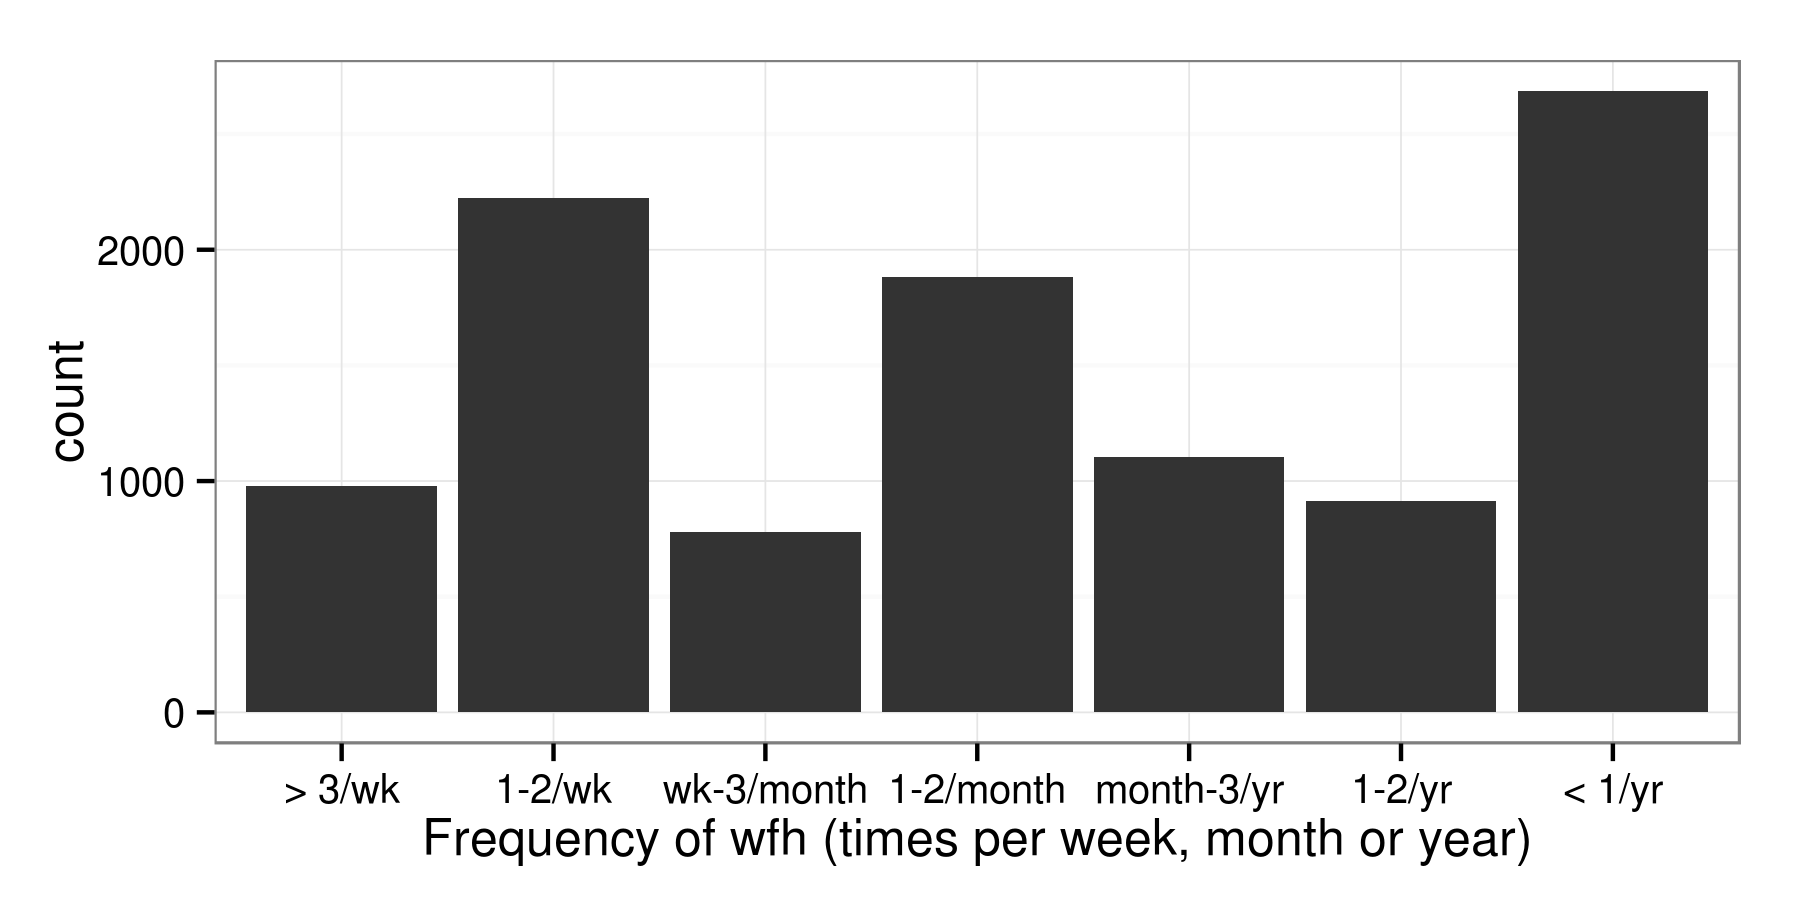
\includegraphics[width=14cm]{freq-nts}
\caption[Bar-plot of frequency of working from home]{Bar-plot of frequency of
working from home (wfh) in the NTS, 2002-2008. Note: only 7\% of the
individual level sample answered this question; around half of the
non-respondents do not work.}
\label{ffreq-nts}
\end{figure}

At the trip level, the NTS contains the following data that can add subtlety
and complexity to our understandings of travel to work. A selection of the
variables that do this are:
\begin{itemize}
 \item D1, J31 and J31A: Journey day and time. This can provide information
about likely level of congestion of work trips on average, and compared with
other trips.
 \item J23: Number of stages. This data mitigates against the simplistic idea,
reinforced by many questionnaires, that all trips consist of only one stage and
one form of transport. The prevalence of multi-stage trips can be investigated
using this variable and, in even finer detail, using the `stages' dataset which
breaks every trip up into its constituent stages.	
 \item JTOTCOST: Total cost of public transport trips. This variable provides
an insight into the costs of public transport and, if the costs of alternative
modes are estimated, the changes that would make more efficient modes more
efficient than driving financially. 
\end{itemize}

`Zooming in' in even further, data on the individual stages taken and vehicles
used for each trip is provided by the NTS in separate files, linked by multiple
(e.g.~household, individual) IDs. The `stages' file 
provides 2.2 million rows of data (only 5\% more than the trips dataset, as
96.7\% of trips taken consist of just a single stage) on occupancy, parking and
even the cost of parking. Clearly, this dataset is invaluable for identifying
the types of multi-stage trip in travel to work, and how these impact on the
energy cost estimates calculated via the assumption that all trips to or from
work consist of just one stage. The `vehicles' dataset contains only 5 types of 
motorised vehicle, including cars, motorcycles/scooter/moped,
``landrover/jeep'', ``light van'' or other. The type of bicycle used to travel
to work is not included, making it impossible to accurately estimate the
embodied energy costs of cycling to work based on the NTS dataset.
Surprisingly, details on the engine size is not provided, although this is not
an issue from an energy use perspective as the CO$_{2}$ band of the vehicle
(which can be converted into energy efficiency estimates) %%%??? Where
is included (in variable V164b). Other relevant variables from the vehicle
dataset include annual mileage (V46), annual commuting mileage (V140) --- these
could be used to determine the extent to which people are dependent on their
cars for commuting, compared with other reasons for trips --- and age of car
(V91a).

The final feature of the NTS dataset to consider is its geographic coverage. It
is a stratified sample within Great Britain. It does contain some geographic
information at the household level, about the type of area in which the
household is based (variable h154a).\footnote{The following 6 categories are
provided:
 Met built-up areas,
 Other urban over 250K,
 Urban over 25K to 250K,
 Urban over 10K to 25K,
 Urban over 3K to 10K,
 Rural.}
Also, the region of each respondent can be inferred by linking individual and
household ids to variable J57G (GOR of trip origin) of the trips dataset.
The NTS dataset has an impressive response rate to key question which tend to
have a lot of NA values, and are very patchy. This would allow an
additional constraint variable to be used for individual level NTS data as an
input into a spatial microsimulation model.

\subsection{Other commuting datasets}
Internationally, the availability of commuting data varies greatly.
This is important, because it can frustrate attempts to compare commuting
patterns across nations. However, if the methods
are to make a major contribution, it should be possible to implement them
worldwide. This depends on access to appropriate data.
Using the aforementioned UK data as a benchmark, Dutch and Colombian datasets
will be evaluated in terms of their suitability for the spatial microsimulation
methods set out below. These datasets were selected because they represent
very different levels of detail, aggregation and availability.

The Dutch data (shown in \cref{sdutchdata}) is provided to the
public\footnote{See {\color{blue}\href{http://statline.cbs.nl/StatWeb/publication/?DM=SLNL&PA=81129ned&D1=0-1,3&D2=0&D3=a&D4=1&D5=0-12&D6=a&HDR=T&STB=G1,G2,G3,G4,G5&VW=T}{http://statline.cbs.nl}},
(full link embedded in the pdf version of this thesis.)} at a
very high level of aggregation. The following attributes are provided for
each mode of transport for each area to two decimal places:
\begin{itemize}
 \item the proportion of all commuters travelling by each mode
 \item average distance of trip
 \item average time per trip
\end{itemize}
The Netherlands data publication policy can be characterised as providing
a very high level of accessibility, but for quite low quality data: it would
not be possible to use this dataset as the basis of a spatial microsimulation
model because, even if socio-demographic constraints were obtained, the
information is provided as averages, telling us nothing about the distribution
of trip distances in each area.
For more detailed geographically aggregated, one would have to
manually aggregate the Dutch equivalent of the National Travel
Survey.\footnote{Piet Rietveld, personal communication.
In fact, there is a plan to do precisely this to provide data to help
explain the differences between English and Dutch energy use, described in
\cref{sinternational}.}
However, the Dutch data does allow for calculation of energy costs, as both
mode, distances and proportions are available (\cref{sinternational}).

On the other extreme, many geo-referenced micro level datasets on
commuting behaviour have been collected. These are generally small in geographical
coverage (at
least relative to the nationwide aggregate level commuting datasets
collected through national censuses) and sometimes in scope also (for example,
it is very common for large organisations to conduct travel surveys of their
staffs' travel patterns). In many cases, a precise geo-reference is allocated
to each individual participating in the survey, although this dataset is generally
not released due to its
sensitivity.\footnote{A
potential case study for this thesis was to take data from the Ordnance Survey's
travel survey as the basis for assessing the energy impacts of organisation level
change. This did not materialise in part due to time constraints and in part
due to concern over access to the geo-referenced individual level data.
}
A very large and detailed example of a geo-referenced individual level dataset
is the \emph{Encuesta de Movilidad de Bogota 2011} \citep{bogota2012}, in which 16,157 `valid'
questionnaires were collected. In addition to questions about travel
(mode, distance and frequency of travel to work and other places), a
range of socio-economic details were collected, including type of housing,
social class, income, `motorisation' (access to cars, motorbikes and bicycles)
and level of education. Unsurprisingly this dataset is not available publicly,
but is available to Colombian researchers with international collaborators
(Ana Moreno Monroy, personal communication). To some extent such a rich dataset
would render the process of generating spatial microdata unnecessary
(although such datasets could be very useful for validation and testing of
these methods). However, the methods of analysis used to interpret the
datasets presented in the latter sections of this chapter and in \cref{s:workdes}
could well be applicable to these valuable micro level datasets.

\section{Geographical data: infrastructure and environment} \label{sadditional}
The datasets presented so far, on energy use of personal travel and commuting
behaviour, are sufficient to calculate the energy costs of commuting at
individual and aggregate levels. The scope of this work extends beyond mere
description, however. Additional input information is required to explain \emph{why}
commuting costs are as they are and to determine the factors likely to
influence the energy costs of commuting beyond those considered so far. These
additional data are classified into infrastructure and topography,
%  geographically inferred data about accessibility
and
remoteness.
%%% May want to say something about additional individual level vars too.

% \subsection{Socio-economic variables} % Add this later
\subsection{Infrastructure}
As discussed further in \cref{scircuity}, the Euclidean distances reported in
the census constraint variable categories (0 - 2 km; 2 - 5 km etc.) are often
not the same as the actual distance travelled to work. This is due to many
reasons, many of them behavioural.
Trip chaining (e.g.~taking a detour on the return journey from
work to do the shopping or on the way there to `drop off the kids'), habitual
use of a certain non-optimum route to work or even preference for
certain parking spaces can all affect circuity. However, infrastructure also
has a large, probably dominant, role to play in determining
how far people \emph{actually} travel to
work relative to the linear distance between home and work. In most cases it is
physically
impossible to travel from A to B in a straight line across an urban area due to
various impassible objects that lie in the way, such as building, fences and
rivers (for all modes of transport) and one-way streets, pedestrianised zones,
prohibitive congestion charges and bollards (for cars). Public transport is the
most constrained geographically, as buses and railed vehicles can only follow
pre-defined paths. Thus, although trains (and to a limited extent buses, when
dedicated bus lanes are present) tend to take more direct routes into the
centre of cities, this does not guarantee that trips by these modes will be
less circuitous than car travel.

Theoretically, the infrastructure on which every mode of transport can usefully
be thought of as a set of points and one-dimensional lines that overlay the
2D geographical surface. %%% Add figure here. And systems of infrastructure
This is reflected in available data on transport
networks: they are
a complex interacting masses of lines (representing the guideways) and points
(intersections between these lines, places to enter the network such as
train and bus stations and motorway link roads). In order to differentiate
between the different transport systems, they can be represented as
completely separate (implicitly non-interacting) layers
(\cref{fnetworks-schematic}). Alternatively,
attributes can be assigned to each
line and point on the entire transport network that includes all nodes and
lines from all networks. These attributes (when present) can be used to
determine the modes that
are able to travel on each, the size of the pathway, information about speed
of travel and, in some cases, direction of travel and other qualities.
With the growth of internet-connected monitoring systems, %% ref
`live' attributes are increasingly feasible (although not yet available in any
dataset the author knows of), such as frequency and destination of departures
and congestion.

\begin{figure}[h]
 \begin{center}
 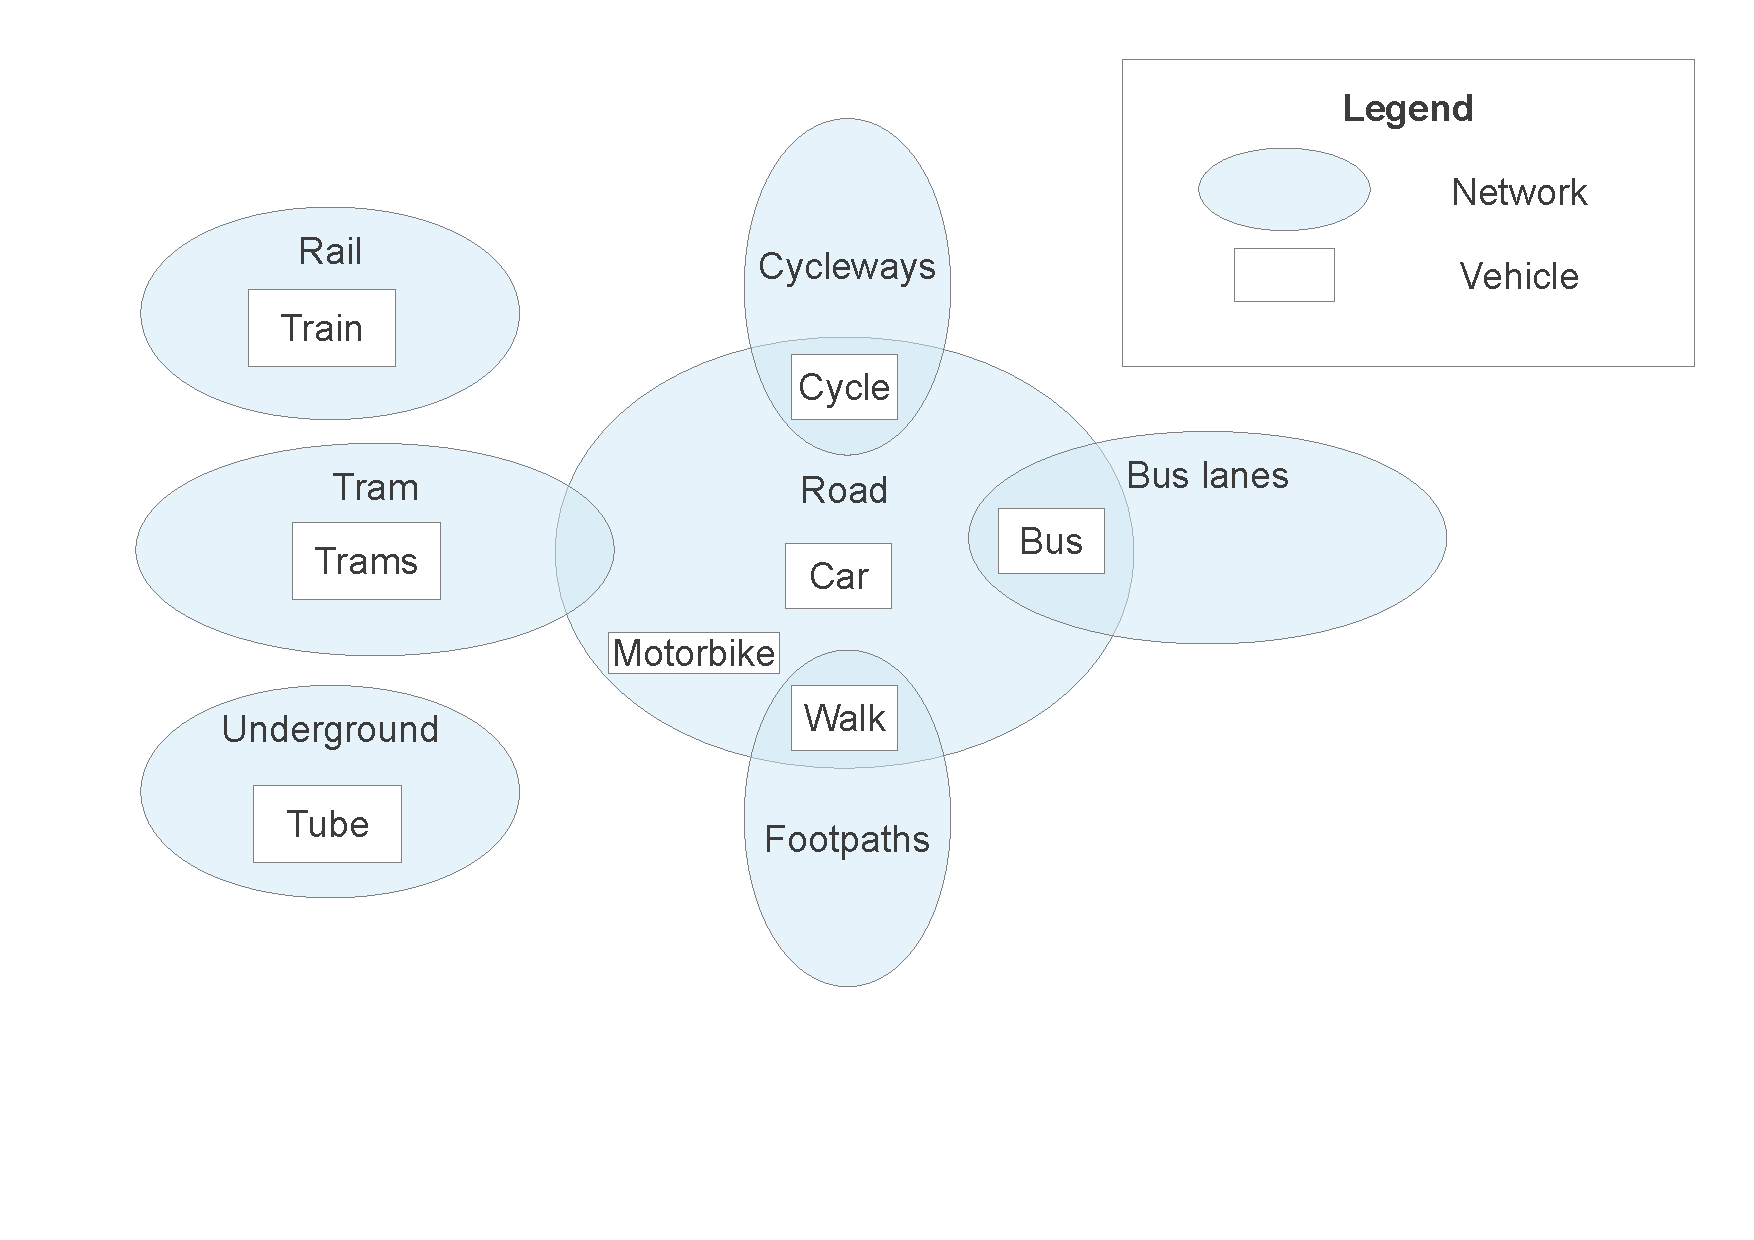
\includegraphics[width=15 cm]{networks-schematic}\end{center}
 % cc-trans.png: 1113x529 pixel, 72dpi, 39.26x18.66 cm, bb=0 0 1113 529
 \caption[Schematic of transport networks and vehicles]{Schematic of main
transport networks used for personal travel and the vehicles that can use them.
Diagram based on \citet{Bolbol2013}.}
 \label{fnetworks-schematic}
\end{figure}


Clearly, this is a complex body of information, and different datasets deal
with it differently (\cref{tnets}). %%% Table on datasets of transport inf.
Only the top three data sources in \cref{tnets} are available free for academic
purposes; these are illustrated in \cref{fosm-trans} to \cref{fitn-master}.
Each of these data sources has its advantages and disadvantages, the most
relevant of which (for the purposes of analysing energy use in personal travel)
will be briefly discussed.



\begin{table}[htbp]
\caption{Comparison of data sources for travel networks}
\begin{tabular}{lp{2cm}p{6 cm}l}
\toprule
Network data source & Networks covered & Key attributes & Availability \\
\midrule
Open Street Map & All & Frequent updated, routing-compatible, official and
unofficial & Free \\
Meridian 2 & Road, rail & Lightweight ($<$ 1 Gb for all UK), national coverage &
Via Edina \\
Mastermap ITN & Road, pedestrian & Large ($\sim$100 Gb for all UK), detailed
with routing & Via Edina \\
ITN Urban Paths & Pedestrian, cycle & Large, detailed map of UK's urban paths
and cycleways & Priced \\ \bottomrule
\end{tabular}
\label{tnets}
\end{table}

\begin{figure}[h]
 \begin{center}
 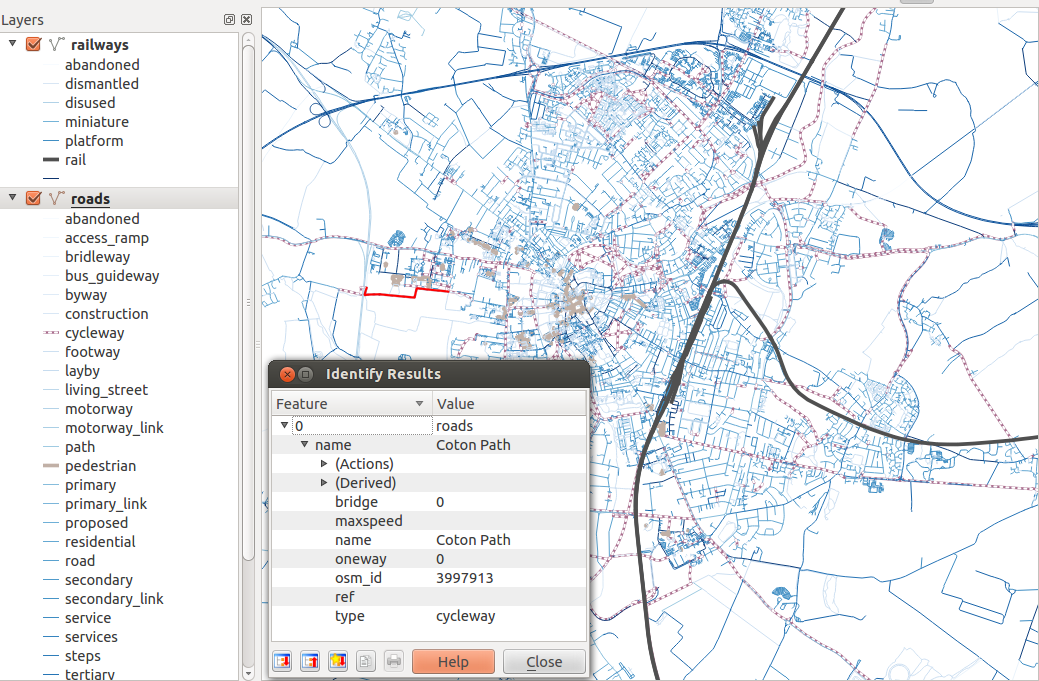
\includegraphics[width=15 cm]{osm-trans}\end{center}
 % cc-trans.png: 1113x529 pixel, 72dpi, 39.26x18.66 cm, bb=0 0 1113 529
 \caption{Visualisation of the OSM data source of the transport network.}
 \label{fosm-trans}
\end{figure}

\begin{figure}[h]
 \begin{center}
 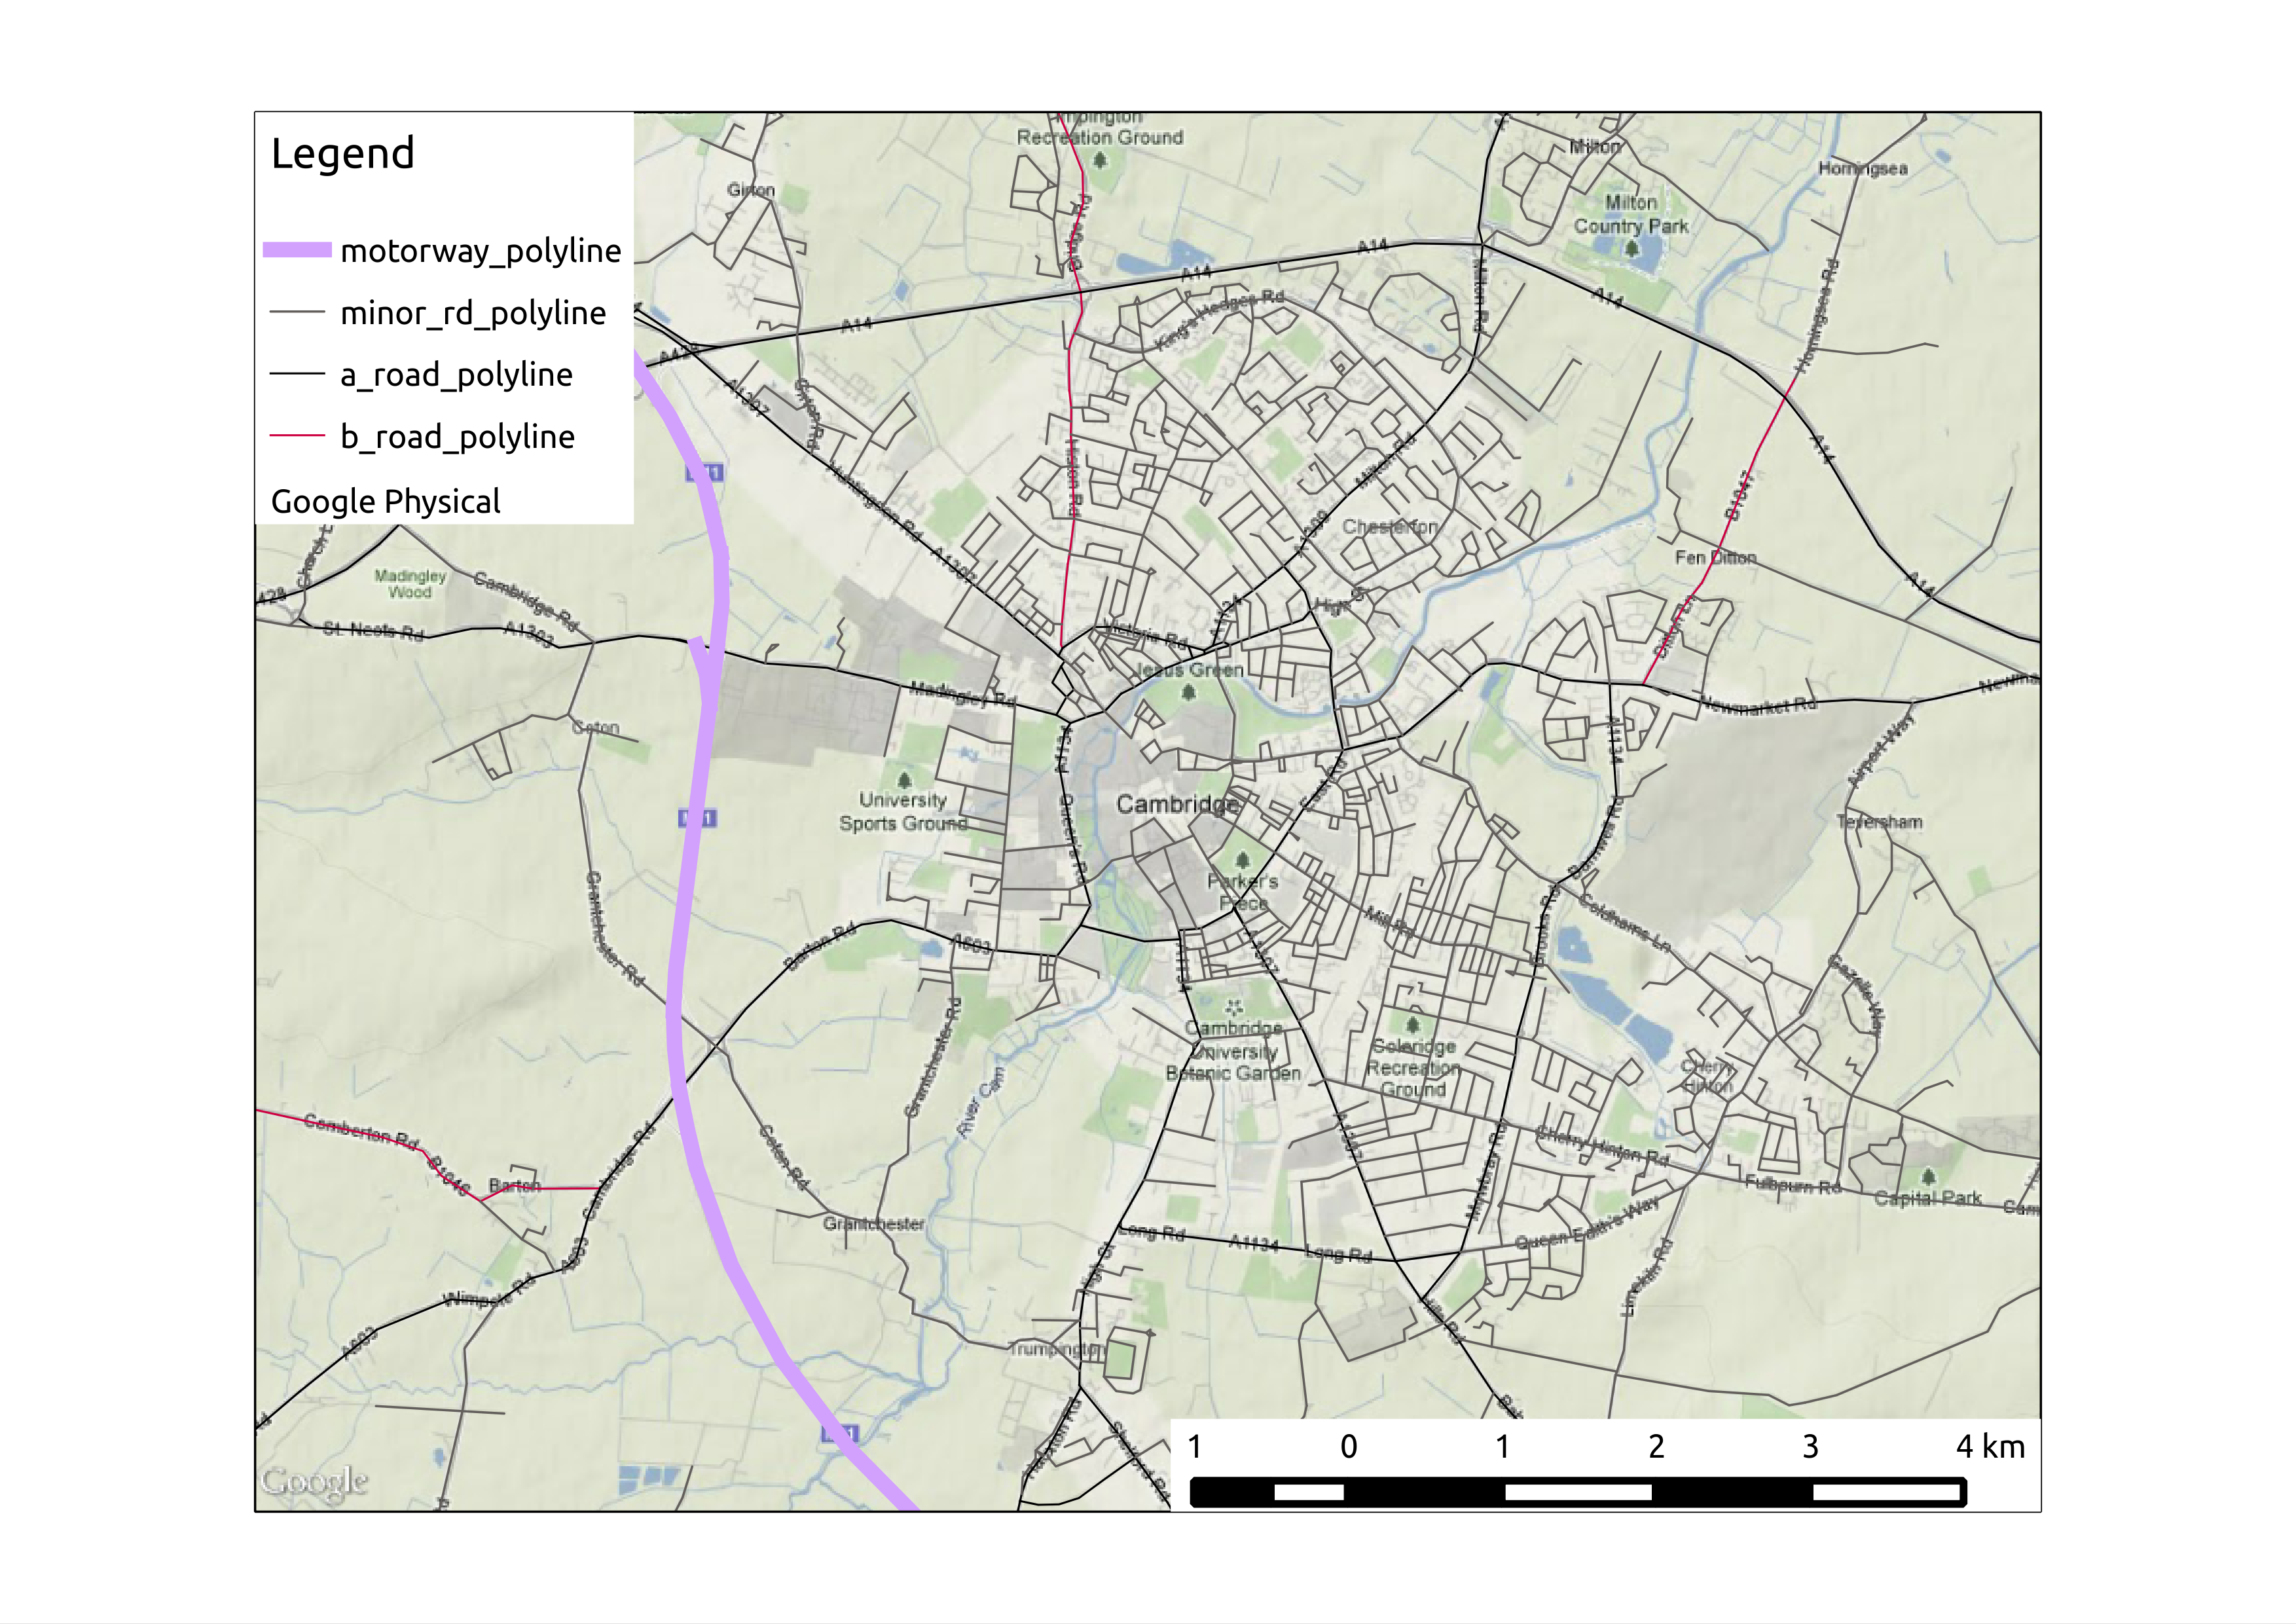
\includegraphics[width=15 cm]{cam-merid2}\end{center}
 % cc-trans.png: 1113x529 pixel, 72dpi, 39.26x18.66 cm, bb=0 0 1113 529
 \caption{The Meridian 2 transport network dataset.}
 \label{fcam-merid2}
\end{figure}

\begin{figure}[h]
 \begin{center}
 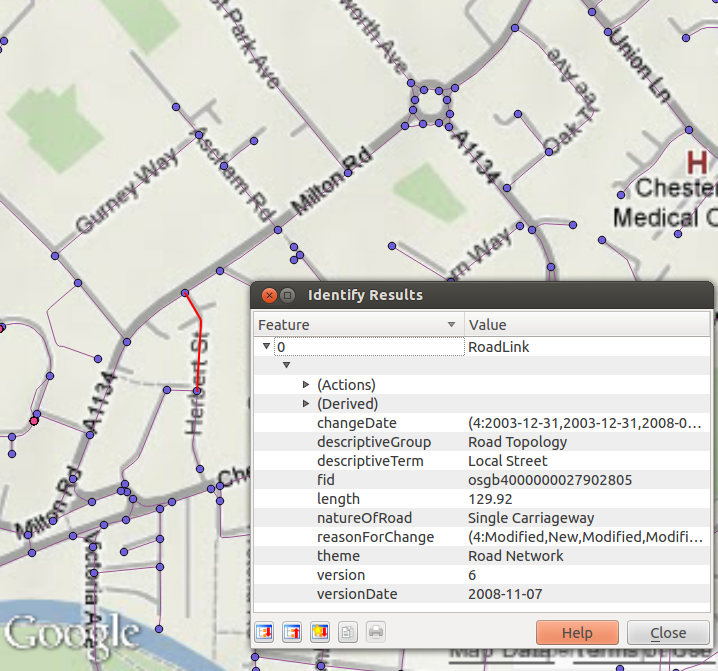
\includegraphics[width=15 cm]{itn-master}\end{center}
 % cc-trans.png: 1113x529 pixel, 72dpi, 39.26x18.66 cm, bb=0 0 1113 529
 \caption{The Ordnance Survey's Integrated Travel Network dataset.}
 \label{fitn-master}
\end{figure}

The Open Street Map dataset is the most suitable `on paper' due to its coverage
of all transport systems in a single file, its level of detail (between the two
free Ordnance Survey offerings: not so large as to make it unwieldy; not too
small to lack detail) and frequent rate of update. Another major advantage of
the OSM dataset is its global coverage: this means that analyses conducted on
it for one country can easily be replicated anywhere in the world. This is not
the case with the Ordnance Survey datasets, as they are proprietary (not
available to non-academic or foreign users) and unique to the UK.

The Ordnance Survey datasets do offer some advantages, however. These can be
summarised as reliability, stability and links to policy makers. All data
entries into the Ordnance Survey system are conducted by professionals who have
been formally trained, and operate to carefully defined standards. OSM data, by
contrast, can be added by anyone with an internet connection. This
`democratisation' of data offers various auxiliary benefits to its participants
\citep{Foresman2008} but also raises issues of data quality. How can one trust
the location and attributes of pathways on a map if they were entered by
amateurs? This is not a question that will be tackled here, but the interested
reader is directed towards the University of Nottingam's OSM-GB (Open Street
Map Great Britain) project\footnote{This project combines OSM data with
information from official sources aims to measure and improve the
quality of the OSM database. See http://www.osmgb.org.uk/ for more detail and
to see their map.} and an academic paper on the subject \citep{Haklay2010}.
\citet{Haklay2010} notes the lack of systematic studies comparing the quality
of traditional and open source (referred to as `volunteered geographic
information') approaches to maps, and sets-out to fill the research gap. It
was found that datasets derived from OSM are generally accurate, especially for large
infrastructures such as motorways, which had an 80\% overlap with the Ordnance
Survey data for 2008 data. However, inconsistencies in the quality of OSM data
were also noted, with rural and deprived areas tending to be more poorly represented in
terms of the existence of objects and the accuracy of their attributes.
Quality of digitisation ranged from ``fairly sloppy in the area of Highgate''
to ``consistent and careful in South Norwood'' \citep[p.~699]{Haklay2010}.
Large errors were far rarer than small ones and overall the OSM
dataset was evaluated as being of `very good' quality.

The second major concern is stability: because the OSM dataset is
continually being updated, it is in constant flux. While most of these changes
are small, and unlikely to alter the results of a particular routing operation,
larger changes do sometimes occur. This is because every aspect of OSM is open
to debate and change. There are, for example, around 5,000 object categories and
growing for OSM objects and users are continuously adding new ones and debating
the structure of the database.\footnote{See
\href{http://wiki.openstreetmap.org/wiki/Map_Features}{
http://wiki.openstreetmap.org/}.} The same issue also applies to the
centralised Ordnance Survey datasets, although these update in a more
systematic manner.

The final point to consider is usability. While OSM datasets are available
worldwide, it is not the standard dataset in use by local planning departments,
which generally have institutional access to Ordnance Survey data. The 
OSM data source is generally also more difficult for non-expert users to find and
download.\footnote{The
OSM transport dataset presented in \cref{fosm-trans}, for example, was not
accessed directly as the .osm file in which the dataset is typically
stored due to problems with downloading, extracting and loading the files in
QGIS. Instead, pre-processed shapefiles, derived from the original OSM data
were downloaded from
{download.bbbike.org}{
http://download.bbbike.org/osm/bbbike/Cambridge/}. Geofabrik.de, and cloudmade
also offer OSM data in forms that are more user friendly for desktop GIS users.
(OSM is well suited to use in geo-databases such as PostGIS.)} Therefore,
one could argue, analyses conducted using the official datasets will be more
likely to be used officially. Of course, this point will vary from organisation
to organisation and methods applicable to one network dataset are generally
applicable to others. In OSM's favour, public administrations in the UK have
recently been recommended to use open source alternatives wherever possible, so
the perception that only official sources are valid may
fade.\footnote{These
recommendations were published in the Government Service Design Manual, as
reported in the story ``New UK government manual for public administrations
promotes open source'' by \href{https://joinup.ec.europa.eu/}{
https://joinup.ec.europa.eu/news/new-uk-government-manual-public-administrations
-promotes-open-source}.}

Consideration of these points led OSM to be the favoured source for most
applications due to its comprehensive coverage of transport networks in a
single file and wide range of attributes for every transport path and node. The
Meridian 2 dataset seems to be best suited for road coverage over large areas
and is ideal for investigating road accessibility of different locations and
network distances by car, as it is available in a handful of polygons for the
entire country. Finally, Ordnance Survey's ITN and Urban Paths layers should be
useful for low level analysis of likely routes of non-motorised modes. However, the
former was found to be difficult to use
% \footnote{97 tiles were downloaded
% for the wider Cambridge area to investigate this dataset. Loading the .gml file
% in QGIS took over a minute and eventually crashed the computer.}
and the latter appears to be unavailable under an academic licence.

\subsection{Topographic data}
Topography is potentially useful both as an explanatory variable of
non-motorised travel and an input into calculations of energy use, due the
addition energy use of driving
uphill compared with driving on the flat.\footnote{This
energy could theoretically
be regained via regenerative breaking. This technology is currently available
in  only a handful of models, and their ``charge/discharge capabilities are
limited'' \citep{Clarke2010}. Due to the added cost and complexity of
regenerative braking systems, their commercialisation for cars and other
vehicles is deemed to be long-way off (if it ever takes off).
}
The extra mechanical energy use of vertical displacement is the same as the
potential energy (PE, measured in Joules) gained by climbing:
\begin{equation}
 PE = mgh
\end{equation}
which is determined by the mass of the vehicle ($m$, in kg), the gravitational
constant ($g$ --- $\sim$10 m/s$^2$ on Earth) and height gained ($h$, in meters).

Topographic datasets for the UK are available from the following sources,
ranging from the coarsest to the finest:
\begin{itemize}
\item The Advanced Spaceborne Thermal Emission and Reflection Radiometer
(ASTER) sensor mounted on the Space Shuttle has produced a dataset that has been
analysed by the Japanese and US space agencies. This has resulted in the Global
Digital Elevation Model Version 2 (GDEM V2). The GDEM has global coverage, a 30
meter resolution, and is free to download from a handful of 
websites, providing a user account and reason for download are
provided.\footnote{See the
following hyperlinks: \href{http://gdex.cr.usgs.gov/gdex/}{cdex.cr.usgs.gov},
\href{http://reverb.echo.nasa.gov/reverb/}{http://reverb.echo.nasa.gov} and
\href{http://www.jspacesystems.or.jp/ersdac/GDEM/E/index.html}
{http://www.jspacesystems.or.jp}. A digital elevation dataset was successfully
downloaded from the first site.} The dataset forms the basis of digital
elevation model used by Google Earth and other Google products.
\item The Ordnance Survey provides height data, either as contour lines or as
interpolated points, for the entirety of the UK and Ireland. The former has a 5
m vertical resolution with an error margin of 2.5 m; the latter has a spatial
resolution of 10 m and an accuracy that depends on the complexity of the
terrain from with points are interpolated.
 \item To improve its flood analysis capabilities, the Environment Agency paid
for a private company to produce high quality LIDAR (light detection and
ranging) data for the majority of the island of Great Britain. The data can be
ordered from the Geomatics website at 25 cm, 50 cm, 1 m, and 2 m resolution, as
either a digital terrain model (DTM, with buildings and vegetation included) or
as a surface model (DSM, representing the `bare' surface). The coverage
increases from less than 1\% for the 25 cm data (for areas most at risk from
flooding) to around 95\% for the 2 m data. The data can be downloaded
commercially for \pounds100 per square kilometre, or free for non-commercial purposes.
\end{itemize}
These datasets were not used directly in the thesis.
Their inclusion could, however, provide background and interesting avenues
for further research for example as a predictor of
the rate of cycling and walking or as a local modifier of energy economy estimates.
% !!! Change this is you use topo data !!!

% \subsection{Estimating accessibility} \label{sgeoinf}
% Some individual level data can be inferred  based on aggregate level data.
% The number of people who commute in the same direction, for example, can be
% derived from commuting flow data provided by Nomis.
% %\footnote{Where to find this
% %data... }
% % by allocating workplace basec on this information.
% This additional level of detail, about \emph{where} people travel to and from
% may well be relevant for decision makers. Simulation of the potential for
% trip sharing or for the increased uptake of non-motorised modes along
% frequently used home-work corridors, for example, could harness this data. The
% `where' question also has strong practical applications, as new infrastructure
% projects such as new bicycle paths rely on data on where people travel from and
% to. The inclusion of direction of commute, via flow data, is tackled in
% \cref{sflow}. This is the type of geographical inference discussed in this
% section, but applied to variables other than those covered by flow--data and
% spatial microsimulation.
% 
% Many variables related to the energy costs of commuting are not
% provided `off the shelf' in official data such as census aggregates. Many of
% these variables (e.g.~average distance to bus stops) have a spatial element, and
% can therefore be inferred from geographic data using computerised calculation.
% Spatial microsimulation performs such inference for individual level variables
% % (hence its alternative name: small area \emph{estimation})
% by combining geographical data, such as that presented in table
% \ref{t:agdata}, with non-geographical microdata (e.g.~see Table \ref{t:indata}).
% This is a central method of the PhD, and is
% described in detail in \cref{setsim}.
% The methods of geographic inference described in this section are simpler. To
% take one example, let us consider the example of proximity to bus stops. As
% mentioned, this is a variable provided at the national level by the NTS, but
% lacks any geographic coverage. Taking an arbitrary Local Authority (data and
% analysis at the national scale would be unwieldy) the input data is available
% from two sources. Open Street Map (OSM) data provides a dynamic yet not
% comprehensive list of bus stops over any area on Earth (Table x). The official
% dataset is more reliable (Table x, Fig. x).
% %%%!!! Priority level: not high. Really good test of speed and skill as qgeo!
% 
% % Other examples: accessibility rank of cycle schemes; public transport
% % Also, 'remoteness' etc sure fit into this section.
% !!! \emph{Here the intention is to highlight explanatory variables and
% quantitative methods} !!!

\subsection{Remoteness} \index{remoteness} \label{sremotness}
% Or area classifications and remoteness or geographically inferred ...
In addition to the transport infrastructure of each area, remoteness was
expected to influence
commuter energy use, primarily via distance travelled and car dependence.
% As outlined in \cref{chapter2}, past literature also supports this hypothesis
% \citep{x,yz}.
%%%! REALLY??? add in cross-ref here.
Intuitively, remote areas are likely to have high energy costs simply by virtue
of the average distance to jobs. Distance to nearest urban centre is a
potentially useful proxy to measure this type of remoteness. This, and
related classification of areas, form the basis of this section.  
The example described applies to medium super output areas (MSOAs) in Yorkshire
and the Humber; the same method could just as easily be applied other
geographies or regions.

The starting point for this is analysis to consider the opposite of remoteness:
living within a city centre. City inhabitants are clearly not isolated in terms
of amenities and social connection, but living in a city does not
actually guarantee proximity to good jobs.\footnote{A good
example of this is Hull, which has the highest unemployment rate of any UK city:
8.7\% ofthe adult population was receiving unemployment benefit as of March 2013
\citep{SimonRog}.
}
To tackle this issue the concept of `employment centre', meaning an area 
with a high concentration of jobs,  was used
against which to measure remoteness. In order to calculate the remoteness of
each MSOA area from employment centres,
it was first necessary to define what constitutes an employment centre and what
does not. Of course, the availability of jobs is not determined by the
Euclidean distance to one dimensional points on the map: employment density
varies continuously over space depending on the location of businesses, schools
and other major employers (\cref{flows2bigemps}). However, employment centres
can provide a neat simplification of reality, a model to simplify and help
understand the complexity of the labour-market commuting interaction.

\begin{figure}[h]
 \begin{center}
 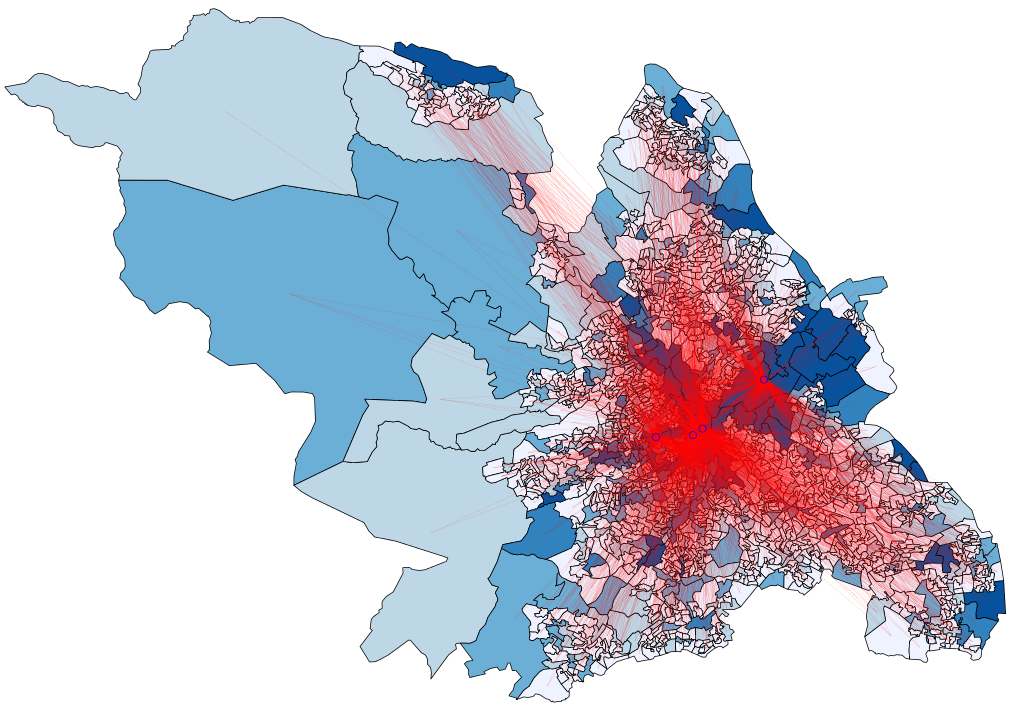
\includegraphics[width=16 cm]{flows2bigemps}\end{center}
 % cc-trans.png: 1113x529 pixel, 72dpi, 39.26x18.66 cm, bb=0 0 1113 529
 \caption[Distribution of employment in Sheffield]{Distribution of employment
in Sheffield, based on flow data from Nomis.
% \cref{sflow}.
Blueness is
proportional to the number of jobs; red lines represent the home-work trips of
people who work in the four Output Areas that employ the most.}
 \label{flows2bigemps}
\end{figure}

Initially, settlements were selected based on their populations. However, the
selection of a threshold population will inevitably be arbitrary and would not
necessarily reflect the employment opportunities of the
area. (On the contrary, one could argue that jobs in some high population areas
would be harder to get and more fought-over than in prosperous countryside
areas.) To overcome this problem, the government's official travel to work areas
(TTWAs) were used. These are defined as geographically contiguous areas within
which 75\% of the population both lives and works \citep{ONS2011-ttw}. They are
named according to the main economic centre(s) within each. In some cases the
TTWAs two main employment centres, as reflected in their name, for example
Malton \& Pickering.

To use these TTWA centres as the basis for distance to work calculations, points
were allocated to the named employment centre(s)
within each TTWA (see the white stars in \cref{fig:dist-ttw-cent}) using
Ordnance Survey's Strategic vector layer of place names. The
next stage was to convert the MSOA areas into points. Care was taken to use the
population-weighted centres of each area, rather than the more commonly used
area-weighted centroids, to reflect distances for typical commuters in each
MSOA. The use of population-weighted centroids reduced the average distance to
employment centres. This is illustrated clearly in the case of ``Ryedale 002''
in North Yorkshire, which extends more than 10 km North of Pickering town centre
(located above the ``i'' in ``Malton and Pickering'') while its population
centre is located less than 2 km from the employment centre, hence the blue
colour.

The algorithm to calculate the distance to the nearest neighbour in a separate
layer is available in QGIS using the Ftools plugin. However, this produced
erroneous results, so the analysis was transferred to R where the function
\verb nncross \ %a
from the package spatstat was used to produce the correct
output. These results were converted back into the vector geographic 
file format of shapefiles using QGIS for plotting. 
The resulting Euclidean distances are depicted in
\cref{fig:dist-ttw-cent}. The variable is interpreted as `distance from
employment centre' and a proxy for remoteness.

\begin{figure}[h]
 \begin{center}
 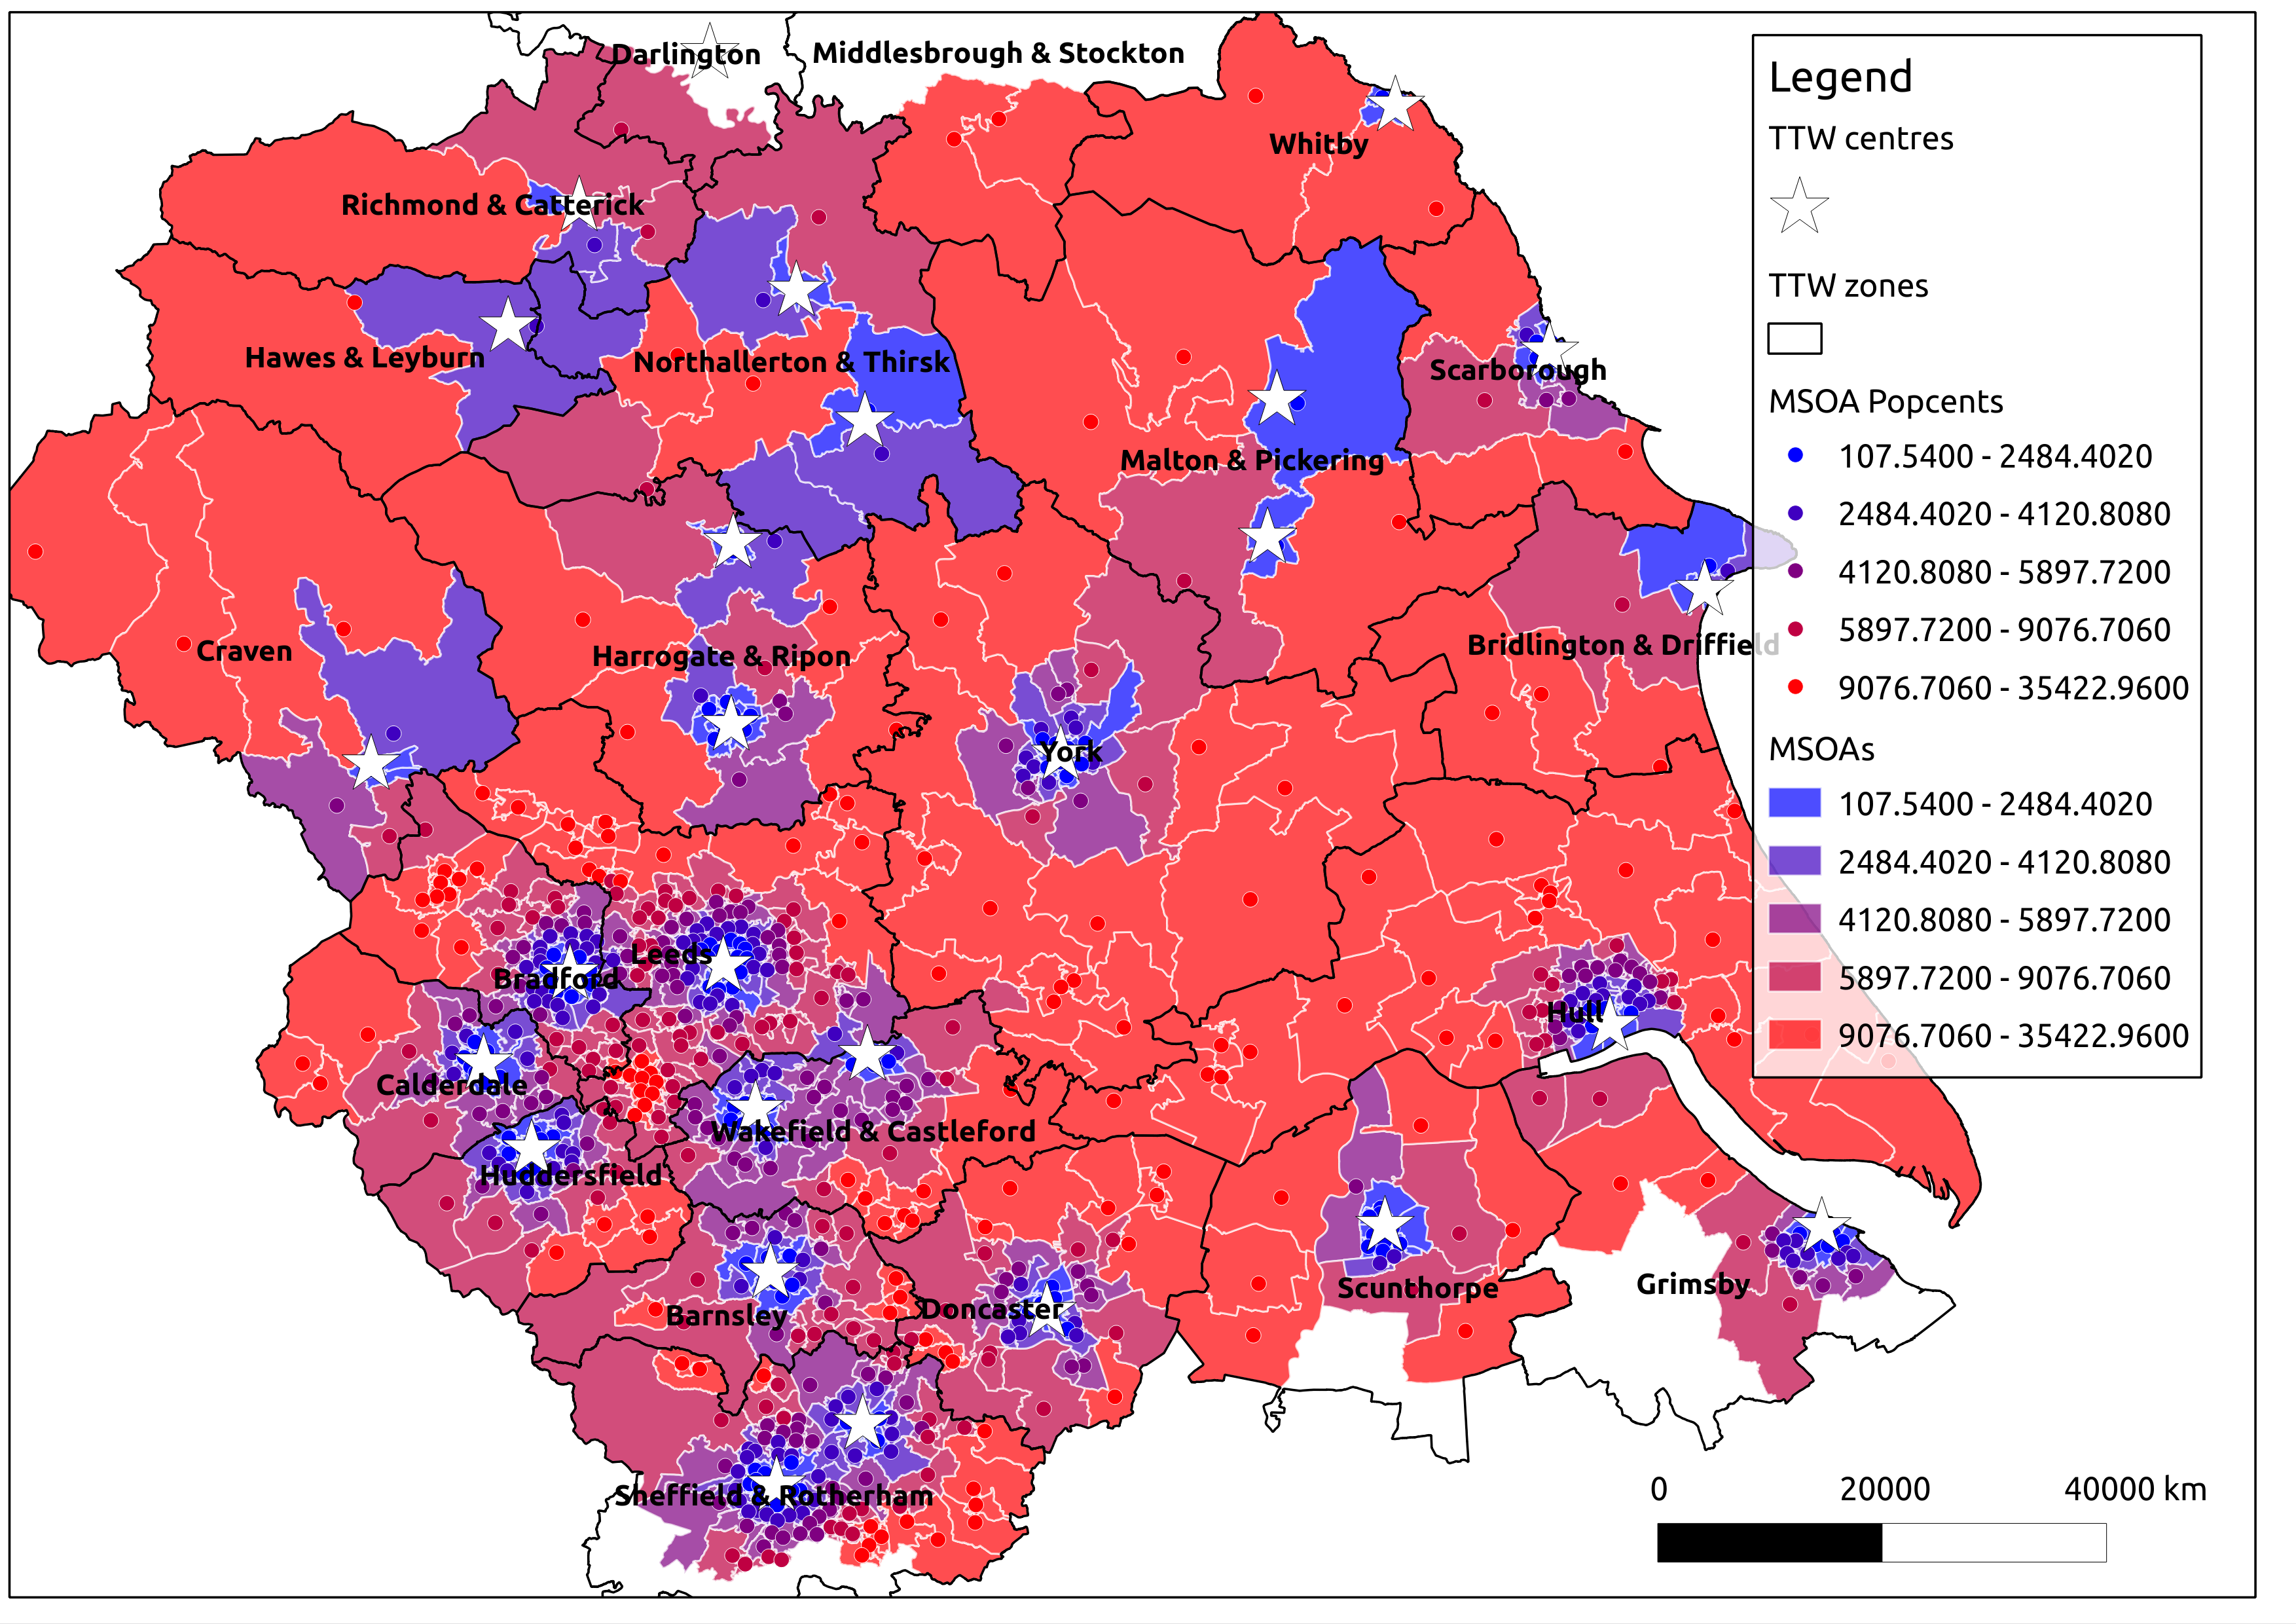
\includegraphics[width=16 cm]{dist-TTW-cent.png}\end{center}
 % cc-trans.png: 1113x529 pixel, 72dpi, 39.26x18.66 cm, bb=0 0 1113 529
 \caption{Illustration of how distance to employment centre was calculated.}
 \label{fig:dist-ttw-cent}
\end{figure}

% !!! Something here about the link between remoteness, rurality and IMD. !!!

\section{Building a spatial microsimulation model in R} \label{setsim}
The previous sections have established the availability of high quality data
on commuting behaviour at geographic and individual levels. Associated
variables such as remoteness and proximity to key transport networks and nodes
can also be inferred based on good geographic data. The challenge now from a
modelling perspective is to join all these elements together.
% Yes but you have not explained how topography/remoteness is included via msim
% methods!!!
Travel to work is
clearly an activity that occurs at the individual level. Overall patterns of
commuting can be expected to be closely related to larger scale processes ---
such as the nature of labour and housing markets, cultural norms and the main
sectors of local economic activity. However, commuting \emph{behaviour} is
always undertaken by individuals making decisions over which they have
some degree of control. %%%!!! Something about agency-structure here?
From short-term choices about at what time to get into work (increasingly
common due to `flexi-time') to strategic decisions about where to live and
work, individuals influence their commuting patterns.

The critical next step, therefore, is to generate spatial microdata on
commuting: individual level data allocated to spatial areas. This is where
spatial microsimulation comes in, to combine the aggregate level commuting
data with the individual level data presented in the previous section.
The technique used in this thesis is Iterative Proportional Fitting (IPF), which
is described in \cref{Chapter3}. The IPF algorithm allocates a weight to each
individual for each area under consideration. If the individual is highly
representative of the area (relative to the individual level dataset) the
weight will increase; if the individual is not representative of the area in
question (or is not present), the weight will decrease.  

As discussed in \cref{Chapter3}, computer hardware has long influenced, and even
\emph{determined} the types of analysis that can be conducted at the individual
level. Hardware limitations are far less of a constraint than they used to be,
elevating the importance of software. As \citet{Holm1987} made clear more than
20 years ago,
% in a section entitled `programming languages',
the choice of software also
has a major impact on the model's flexibility, efficiency, reproducibility and
ease of coding. It was noted that ``little attention is paid to the
choice of programming language used'' \citep[p.~153]{Holm1987}, an observation
that appears to be as true now as it was then. % Search for languages? no.???
For this research, a conscious decision was made early on to use R, and this
has had an impact on the model construction, features, analysis and even design
philosophy. It is at this stage, therefore, that R as a platform for undertaking
spatial microsimulation is discussed in some detail. The theory is discussed in
\cref{s:theory}

\subsection{Why R?}
The majority of the quantitative analysis conducted for this thesis, and the
entirety of the spatial microsimulation model used, was written in R. This was
a deliberate choice made at the outset rather than an arbitrary decision based
on predecessors. This section briefly explains the importance of choosing
appropriate computer software in academic research in general, with respect to
reproducibility, a cornerstone of science. The choice of R in particular is then
described. R was chosen for its virtues, which are summarised well in
\citet{Matloff-R}:

\begin{itemize}
\item ``a public-domain implementation of the widely-regarded S statistical
language; R/S is the de facto standard among professional statisticians
\item comparable, and often superior, in power to commercial products in most
senses
\item available for Windows, Macs, Linux
\item in addition to enabling statistical operations, it's a general programming
language, so that you can
automate your analyses and create new functions
\item object-oriented and functional programming structure
\item your data sets are saved between sessions, so you don't have to reload
each time
\item open-software nature means it’s easy to get help from the user
community''
\end{itemize}

\citet{Matloff-R} also provides five
examples of the type of people who would be interested in programming in R,
rather than using it as a quick and easy tool for graphing and numerical
analysis. Of particular relevance to this thesis is the second of Matloff's 
categories of people for whom R is recommended:
``Academic researchers developing statistical methodology that is either new or
combines existing methods into an integrated procedure that needs to be codified
for usage by the general research community'' \citep[p.~xiii]{Matloff-R}.

The quote also suggests some of the potential advantages of writing multi-use
scripts in R rather than a collection of unrelated functions: by its
very nature modelling is an iterative exercise, so it is important to be able
to invoke specific chunks of code (e.g.~using the \verb source() ~command) that
are modular. While this capability is not unique to R, the range of statistical functions that
can be performed within a unified environment is. The
rapidly growing use of R for spatial data analysis was another factor that
makes it well-suited to spatial-microsimulation and other types of geographic
modelling (e.g.~\citealp{Singleton2013-school}). R overcomes the need to switch
between several different programs (e.g.~one for analysis, one for graphing,
one for mapping), increasing simplicity and (eventually) productivity.

Despite all these advantages, R has a number of weaknesses itemised below along with techniques and projects which mitigate them:
\begin{itemize}
 \item R loads everything into RAM. This can be problematic when querying
 large datasets, of which only one part needs to be accessed at a
 time.\footnote{ This is especially common with geographical analysis, which often focus
 on a small area of a large map at a time \citep{Obe2011}.
 }
 There are numerous tools
 that overcome this constraint by querying databases (stored on the hard-disk) from within R, including
 RMySQL \citep{james2012rmysql} and Rattle \citep{Williams2009}. \citet{Singleton2013-school}
 queried a PostGIS database from within R to estimate the route taken by school
 commuters, for the estimation of associated CO$_2$ emissions.
 \item R can be slow, for example running for loops and when used as a general programming
 language which is not R’s main purpose. R being an
 interpreted language there are times when the performance advantages of a compiled language such as 
 C/C++ are needed.
 To this end the RCPP package was developed, which provides
 ``Seamless R and C++ integration''  \citep{eddelbuettel2011rcpp}. Packages are also available
 to integrate R with Java (rJava), Python (rpy2) and text markup languages such as Markdown and
 \LaTeX (knitr). Also, the base installation of R provides an inbuilt C compiler for doing the
 `heavy lifting' tasks such as kernel density estimation \citep{peng2002introduction}.
 These links to other languages could be useful for porting pre-existing algorithms
 for spatial microsimulation into R (e.g.~\citealp{Williamson2007, Ballas2007simb}).
 \item R's base graphics are unattractive and unintuitive. This problem has been
 tackled most comprehensively in a PhD thesis by Hadley Wickham \citep{Wickham2008}.
 The aim was to implement the `grammar of graphics' \citep{wilkinson2005grammar},
 a comprehensive and coherent approach to data visualisation, into an existing
 open-source statistical programming language. The result is ggplot2,
 which has a very active user and developer community \citep{wickham2011ggplot2}.
 ggplot2 has been used throughout this thesis for plotting with help from key
 references \citep{wickham2011ggplot2, chang2012r}.
 \item R's visualisations are not dynamic. This problem has been partly
 overcome in the realm  of GIS with two QGIS plugins: ManageR and Home range.
 For dynamic web applications, the R package Shiny provides similar interactive
 functionality as Google's Fusion tables project. There is also a nascent
 interface between R and Processing (rprocessing), an abstraction of Java
 ideal for dynamic
 visualisations of geographic data (e.g.~\citealp{wood2010visualisation}).
\end{itemize}


\subsection{IPF theory: a worked example} \label{s:theory}
In most modelling texts there is a strong precedence of theory over
application: the latter usually flows from the former. The location 
of this section after a description of the programming language
R is therefore a little unconventional but there is a logic to this order. 
Having demonstrated the power and flexibility of the programming language in
which the model is written, the next stage is to analyse the task to which it
is to be set. More importantly for reproducible research, this theory section
is illustrated with a simple worked example that culminates in
a question to the reader, to test his or her understanding.

IPF is a simple statistical procedure, ``in which cell counts in a contingency
table containing the sample observations are scaled to be consistent with
various externally given population marginals'' \citep{mcfadden2006testing}. In
other words, and in the context of \emph{spatial} microsimulation, IPF produces
maximum likelihood estimates for the frequency with which people appear in
different areas. The method is also known as `matrix raking' or the RAS
algorithm, (\citealp{Birkin1988, Muller2010,
Simpson2005, Kalantari2008, Jirousek1995}) and has been described as one
particular instance of a more general procedure of `entropy maximisation'
\citep{Johnston1993, blien1998entropy}.
The mathematical properties of IPF
have been described in several papers
(\citealp{Bishop1975, Fienberg1970, Birkin1988}).
Illustrative examples of the procedure can be found in
\citet{Saito1992}, \citet{Wong1992}
and \citet{Norman1999a}. \citet{Wong1992} investigated the reliability of IPF
and evaluated the importance of different factors influencing the its
performance. Similar methodologies have since been employed by
\citet{Mitchell2000}, \citet{Williamson2002} and
Ballas et al.~\citeyearpar{Ballas2005c, Ballas2005}
to investigate a wide range of phenomena.

% As \citet{Birkin1988} point out, IPF undertakes the basic task of
% generating a vector of individual characteristics, $x = (x_1, x_2, ..., x_m)$ on the
% basis of a joint probability distribution $p(x)$. Once the probability distribution
% for such a vector is generated, representative
% individuals can be synthesised or extracted from a pre-existing survey dataset.
% However, when information is not available for the full joint distribution, there
% is a need to construct a product of conditional and marginal probabilities,
% by building one attribute at a time, so that the probability of certain attributes
% is conditionally dependent on existing attributes \citep{Birkin1988}:
%
% \begin{equation}
% p(x) = p(x_1)p\left( \frac{x_2}{x_1}\right) p\left( \frac{x_3}{x_2}, x_1\right) \times
%  ... \times p\left( \frac{x_m}{x_{m-1}},...,x_1\right)
% \end{equation}
%
% IPF can be used to model the joint probability distribution
% $p(x_1, x_2, x_3)$ subject to known probabilities
% $p(x_1, x_2)$ and $p(x_1, x_3)$. Following \citet{Birkin1988} and \citet{Ballas2007simb},
% if $p(x_1, x_2, x_3)$ is the $i^{th}$ approximation to the three-attribute joint probability
% vector then:
% \begin{equation}
%  p^1(x_1, x_2, x_3) = \frac{1}{N_1 N_2 N_3}
% \end{equation}
% where $N_j$ is the number of possible states associated with the attribute vector $x$.
% The vector can then be adjusted in \emph{proportion} to the following known constraints:
% \begin{equation}
% p^2(x_1, x_2, x_3) = p^1(x_1, x_2, x_3) \frac{p(x_1, x_2)}
% {{\displaystyle \sum^{}_{x_3}{p^1(x_1, x_2, x_3)}}}
% \label{eq:p2}
% \end{equation}
% \begin{equation}
% p^3(x_1, x_2, x_3) = p^2(x_1, x_2, x_3) \frac{p(x_1, x_3)}
% {{\displaystyle \sum^{}_{x_2}{p^1(x_1, x_2, x_3)}}}
% \label{eq:p3}
% \end{equation}
% IPF involves iterating through equations \ref{eq:p2} and \ref{eq:p3}
% until a \emph{fitted} distribution is obtained, when the probabilities
% are convergent within some acceptable limit \citep{Birkin1988, Fienberg1970, Ballas2007simb}.
% This procedure can be generalised to a larger number of attributes \citep{Birkin1988}:
% if we let $Z_k(x)$ be a subset of the set of attribute vectors
% $E(x)$ for which marginal joint probabilities are known and let $W_k(x)$ be
% the complement of $Z_k(x)$, that is $W_k(x)= E(x) - Z_k(x)$, then:
%
% \begin{equation}
%  p^1(x) = \frac{1}{\displaystyle{\prod^{m}_{i=1}{Ni}}}
% \end{equation}
% \begin{equation}
%  p^2(x) =  p^1(x) \frac{p[Z_1(x)]}{\displaystyle{\sum^{}_{W_1(x)}{p^1(x)}}}
% \label{eq:six}
% \end{equation}
%
% {\centering
% .
%
% .
%
% .
%
% }
%
% \begin{equation}
%  p^{k+1}(x) =  p^k(x) \frac{p[Z_k(x)]}{\displaystyle{\sum^{}_{W_k(x)}{p^k(x)}}}
% \label{eq:seven}
% \end{equation}
%
% IPF iterates through equations \ref{eq:six} and \ref{eq:seven} until convergence
% \citep{Birkin1988}. An extensive discussion of the mathematical properties of
% IPF can be found in \citet{Fienberg1970}.

To illustrate how IPF works in practice, a simplified example is described below.
This is a modified version of a simpler demonstration from
\citet{Ballas2005}.\footnote{In \citet{Ballas2005}
the interaction between the age and sex constraints are assumed to be known.
(Their equivalent of \cref{t:s2} contains data for every cell,
not question marks.) This results in IPF converging instantly.
However, in Census data, such cross-tabulation is
often absent, and IPF must converge over multiple constraints and
iterations. This latter scenario is assumed in the worked example below. Other
worked examples of the principles are provided in \citet[Appendix
3]{johnston1985geography} (for entropy maximisation), \citet{Norman1999a} and
\citet{Simpson2005} (using the proprietary statistical software SPSS).
}
Table \ref{t:w}  describes a
hypothetical microdataset comprising 5 individuals, who are defined by two
constraint variables, age and sex. Each has two categories.
Table \ref{t:s} contains aggregated data
for a hypothetical area, as it would be downloaded from census dissemination
portal Casweb. \Cref{t:s2} illustrates this table in a different form,
which shows our ignorance of interaction between age and sex.


\begin{table}[h]
\centering
\caption[A hypothetical input microdata set]{A
hypothetical input microdata set (the original
weights set to one). The bold value is used subsequently for
illustrative purposes.}
\begin{tabular}{llll}
\toprule
{Individual } & {Sex} & {Age-group} & {Weight} \\
\midrule
1 & Male & Over-50 & 1 \\
2 & Male & Over-50 & 1 \\
3 & {Male} & {Under-50} & \textbf{1} \\
4 & Female & Over-50 & 1 \\
5 & Female & Under-50 & 1 \\
\bottomrule
\end{tabular}
\label{t:w}
\end{table}
\vspace{1cm}


\begin{table}[htbp]
\centering
\caption{Hypothetical small area constraints data ($s$).}
\begin{tabular}{cllll}
\toprule
Constraint $\Rightarrow$ & \multicolumn{2}{c}{$i$}& \multicolumn{2}{c}{$j$}\\
Category $\Rightarrow$ & $i_1$ & $i_2$ & $j_1$ & $j_2$ \\
Area $\Downarrow$  & Under-50 & Over-50 &  Male & Female\\
1  & 8 & 4 & 6 & 6\\
\bottomrule
\end{tabular}
\label{t:s}
\end{table}
\vspace{1cm}

\begin{table}[htbp]
\centering
\caption[Small area constraints expressed as marginal totals]{Small
area constraints expressed as marginal totals, and the cell
values to be estimated.}
\begin{tabular}{cllll}\toprule
Marginal totals&  & \multicolumn{2}{c}{$j$} & \\
& Age/sex & Male & Female & T\\ \midrule
\multirow{2}{*}{$i$} & Under-50 & \textbf{?} & ? & 8\\
& Over-50 & ? & ? &4 \\
& T & 6 & 6 &12\\
\bottomrule
\end{tabular}
\label{t:s2}
\end{table}

Table \ref{t:m} presents the
hypothetical microdata in aggregated form,
that can be compared directly to Table \ref{t:s2}.

\begin{table}[htbp]
\centering
\caption[The aggregated results of the weighted
microdata set]{The aggregated results of the weighted
microdata set ($m(1)$).
Note, these values depend on the
weights allocated in Table \ref{t:w} and therefore
 change after each iteration}

\begin{tabular}{cllll}\toprule
Marginal totals&  & \multicolumn{2}{c}{$j$} & \\
& Age/sex & Male & Female & T\\ \midrule
\multirow{2}{*}{$i$} & Under-50 & \textbf{1} & 1 & 2\\
& Over-50 & 2 & 1 &3 \\
& T & 3 & 2 &5\\
\bottomrule
\end{tabular}
\label{t:m}
\end{table}

Using these data it is possible to readjust the weights of the hypothetical
individuals, so that their sum would add up to the totals given in Table
\ref{t:s2} (12). In particular, the weights can be readjusted by multiplying them by
the marginal totals, originally taken from
Table \ref{t:s} and then divided by the respective marginal total in \ref{t:m}.
Because the total for each small-area constraint is 12, this must be
done one constraint at a time. This
can be expressed, for a given area and a given constraint ($i$
or age in this case), as follows:

\begin{equation}
w(n+1)_{ij} = \frac{w(n)_{ij} \times sT_{i}}{mT(n)_{i}}
\label{eq:ipf}
\end{equation}
where $w(n+1)_{ij}$ is the new weight for individuals with characteristics $i$
(age, in this case), and $j$ (sex),  $w(n)_{ij}$ is the original
weight for individuals with these characteristics, $sT_{i}$ is element
marginal total of the small area constraint, $s$
(Table \ref{t:s}) and $mT(n)_{i}$ is the marginal total of category
$j$ of the aggregated results of the weighted
microdata, $m$ (Table \ref{t:m}). $n$ represents the iteration number.
Although the marginal totals of $s$ are known, its cell values
are unknown. Thus, IPF estimates the interaction (or cross-tabulation)
between constraint variables.
(Follow the emboldened values in the tables
to see how the new weight of individual 3 is calculated for the sex constraint.)
Table \ref{t:new-weights} illustrates the weights that result. Notice that the
sum of the weights is equal to the total population, from the constraint variables.

\begin{table}[htbp]
\centering
\caption{Reweighting the hypothetical microdataset in order to fit
Table \ref{t:s}.}
\begin{tabular}{lllll}
\toprule
{Individual} & {Sex} & {age-group} & {Weight} &
{New weight, w(2)} \\ \midrule
1 & Male & Over-50 & 1 & $1 \times 4/3 = \frac{4}{3}$ \\
2 & Male & Over-50 & 1 & $1 \times 4/3 = \frac{4}{3}$ \\
3 & Male & Under-50 & 1 & $\textbf{1} \times
\textbf{8}/\textbf{2} = 4$ \\
4 & Female & Over-50 & 1 & $1 \times 4/3 = \frac{4}{3}$ \\
5 & Female & Under-50 & 1 & $1 \times 8/2 = 4$ \\
\bottomrule
\end{tabular}
\label{t:new-weights}
\end{table}

After the individual level data have been re-aggregated (\cref{t:m2}),
the next stage is to repeat \cref{eq:ipf} for the age constraint to generate a
third set of weights, by replacing
the $i$ in $sT_{i}$ and $mT(n)_{i}$ with $j$ and incrementing the value of n:

\begin{equation}
w(3)_{ij} = \frac{w(2)_{ij} \times sT_{j}}{mT(2)_{j}}
\label{eq:ipf2}
\end{equation}

To test your understanding of IPF, apply \cref{eq:ipf2} to the information above
and that presented in \cref{t:m2}.
This should result in the following vector of new weights, for individuals 1 to 5:
\begin{equation}
%  w(3) = (\frac{6}{5}, \frac{?}{?}, \frac{18}{5}, \frac{?}{?}, \frac{9}{2})
  w(3) = (\frac{6}{5}, \frac{6}{5}, \frac{18}{5}, \frac{3}{2}, \frac{9}{2})
\end{equation}
As before, the sum of the weights is equal to the population of the area (12).
Notice also that after each iteration the fit between the marginal
totals of $m$ and $s$
improves. The total absolute error (TAE, see \cref{etae} below)
from $m(1)$ to $m(2)$ improves from
14 to 6 in \cref{t:m} and \cref{t:m2} above. TAE for $m(3)$ (not shown,
but calculated by aggregating $w(3)$) improves even more, to 1.3.
This number would eventually converge to 0 through subsequent
iterations, as there are no empty cells in the input microdataset;
a defining feature of IPF.


\begin{table}[htbp]
\centering
\caption[Aggregated results after constraining for age]{The
aggregated results of the weighted
microdata set after constraining for age ($m(2)$).
}

\begin{tabular}{cllll}\toprule
Marginal totals&  & \multicolumn{2}{c}{$i$} & \\
& Age/sex & Male & Female & T\\ \midrule
\multirow{2}{*}{$j$} & Under-50 & 4 & 4 & 8\\
& Over-50 & $\frac{8}{3}$ & $\frac{4}{3}$ & 4 \\
& T & $6\frac{2}{3}$ & 5$\frac{1}{3}$ & 12\\
\bottomrule
\end{tabular}
\label{t:m2}
\end{table}

The above process, when applied to more categories (e.g. socio-economic class)
and repeated iteratively until a satisfactory convergence occurs, results in a
series of weighted microdatasets, one for each of the small areas being
simulated. This allows for the estimation of variables whose values are not
known at the local level (e.g. income) \citep{Ballas2005}. An issue
with the results of IPF (absent from combinatorial optimisation methods),
however, is that it results in non-integer weights: fractions of individuals
appear in simulated areas. As described in the introduction, this is not ideal
for certain applications. Integer weights allow the results of spatial
microsimulation to be further processed using dynamic microsimulation and agent
based modelling techniques \citep{Pritchard2012}.


% A key benefit from a policy perspective is that
% IPF and other spatial microsimultion techniques
% can provide estimation of variables whose values are not
% known at the local level (e.g. income).
Spatial microsimulation can also provide insight into the likely
distribution of individual level variables about which only
geographically aggregated statistics have been made available.
An issue
with the results of IPF (absent from combinatorial optimisation methods),
however, is that it results in non-integer weights: fractions of individuals
appear in simulated areas.

\subsection{Implementing IPF in R} \label{simplementing}
The above example is best undertaken by hand, probably with a pen and paper
to gain an understanding of IPF, before the process is automated for 
larger datasets. This section explains how the IPF
algorithm described above was implemented in R, using a slightly more
complex example.
% This section is based on ``Spatial microsimulation in R: a
% beginner’s guide to iterative proportional fitting (IPF)'', a tutorial
% written to accompany a methods paper on integerisation
\citep{Lovelace2013-trs}.\footnote{This tutorial is available from Rpubs, a site dedicated
to publishing R analyses that are reproducible. It uses the RMarkdown
mark-up language, which enables R code to be run and presented within
documents. See http://rpubs.com/RobinLovelace/5089 \label{fnrpub} .}

\emph{Loading in the data}

In the full model the input datasets are stored as .csv files, one for each
constraint and one for the input microdata, and read in with the command
\verb read.csv . For the purposes of understanding how the model works,
the dataset is read line by line, following the
example above. The following code creates example datasets,
based on the same hypothetical survey of 5 individuals described above,
and 5 small areas. The spatial microsimulation model will select individuals
based on age and sex and mode of transport (mode of transport
is also used on the larger online example described in footnote \ref{fnrpub}).
For consistency with the (larger) model used for the paper, 
the individual level data will be referred to as USd (Understanding Society dataset)
and the geographic data as all.msim (for all constraint variables).
The code to read-in the individual level data are presented in code sample \ref{cusd}.
When called, the data are then displayed as a table (see listing \ref{cout}).
\begin{lstlisting}[float=h, caption={Manual input of individual level data
in R}, label=cusd]
# Read in the data in long form (normaly read.table() used)
c.names <- c("id", "age", "sex")
USd <- c(       1, 59, "m",
                2, 54, "m",
                3, 35, "m",
                4, 73, "f",
                5, 49, "f")
USd <- matrix(USd, nrow = 5, byrow = T) # Long data into matrix
USd <- data.frame(USd) # Convert this into a dataframe
names(USd) <- c.names # Add correct column names
USd$age <- as.numeric(levels(USd$age)[USd$age]) # Age is a numeric
\end{lstlisting}
\begin{lstlisting}[float=h, caption={Output of the USd data frame}, label=cout]
USd # Show the data frame in R
##   id age sex
## 1  1  59   m
## 2  2  54   m
## 3  3  35   m
## 4  4  73   f
## 5  5  49   f
\end{lstlisting}
The same procedure applies to the geographical data (listing \ref{cgeo}).
\begin{lstlisting}[float=h*, caption={Geographic data input}, label=cgeo]
 category.labels <- c("16-49", "50+" # Age constraint
             ,"m", "f" # Sex constraint
             # more constraints could go here
             )
all.msim <- c(  8, 4,    6, 6,   # Original aggregate data
                2, 8,    4, 6,   # Elderly
                7, 4,    3, 8,   # Female dominated
                5, 4,    7, 2,   # Male dominated
                7, 3,    6, 4    # Young
                )
all.msim <- matrix(all.msim, nrow = 5, byrow = T) 
all.msim <- data.frame(all.msim) # Convert to dataframe
names(all.msim) <- category.labels # Add correct column names
\end{lstlisting}

IPF relies on the assumption that all constraint variables will contain the
same number of people. This is logical (how can there be more people classified
by age than by sex?) but can cause problems for constraint variables that use
only a subset of the total population, such as those who responded to questions on
travel to work. To overcome this problem, it is possible to normalise the
constraint variables, setting the total for each to the one that has the most
reliable total population. This worked example simply checks whether
or not they are (listing \ref{ccheck}).

\begin{lstlisting}[float=h, caption={R code to check the constrain populations
match}, label=ccheck]
 # Check totals for each constraint match
rowSums(all.msim[,1:2]) # Age constraint
## [1] 12 10 11  9 10
rowSums(all.msim[,3:4]) # Sex constraint
## [1] 12 10 11  9 10

rowSums(all.msim[,1:2]) == rowSums(all.msim[,3:4])
## [1] TRUE TRUE TRUE TRUE TRUE
\end{lstlisting}

\emph{Reweighting the survey dataset}

Iterative proportional fitting determines the weight allocated to each
individual for each zone to best match the geographically aggregated data.
A weight matrix is therefore created, with rows corresponding to individuals
and columns to zones, as described in \cref{s:theory}. In
R, this, and the creation of the aggregated results matrix,
is done with code presented in listing
\ref{cws}).\footnote{In subsequent
versions of the model, single, multi-dimensional weight and
aggregated result matrices are used,
to reduce the length of the scripts.
} 

\begin{lstlisting}[float=h, caption={Creating arrays of weights in R},
label=cws]
weights0 <- array(dim=c(nrow(USd),nrow(all.msim)))
weights1 <- array(dim=c(nrow(USd),nrow(all.msim)))
weights2 <- array(dim=c(nrow(USd),nrow(all.msim)))

weights0[,] <- 1 # sets initial weights to 1

USd.agg <- array(dim=c(nrow(all.msim),ncol(all.msim)))
USd.agg1 <- array(dim=c(nrow(all.msim),ncol(all.msim)))
USd.agg2 <- array(dim=c(nrow(all.msim),ncol(all.msim)))
colnames(USd.agg1) <- category.labels
\end{lstlisting}

It is important to note that in real survey data, the variables are not
always neatly categorised into the same bins as the levels of the aggregate
data. Age, for example can be classified in many different ways.
Also, a wide form is useful for subsequent steps.
Therefore, it is necessary to convert the `thin' survey dataset
into a wider form, by converting a single column such as age or sex into
multiple columns corresponding to the number of categories. Sometimes the
cut-off points of the categories can be decided (as with age), or categories
can be merged (when many different NA options are available, for example).
The code that performs this important process for our example dataset is
presented in listing \ref{ccat}.

\begin{lstlisting}[float = h, caption={R code to convert the survey
dataset into binary form}, label=ccat]
USd.cat <- array(rep(0), dim=c(nrow(USd),
			  length(category.labels !=0)))

USd.cat[which(USd$age < 50),1] <- 1 # Age, "< 50"
USd.cat[which(USd$age >= 50),2] <- 1 # "50+"
USd.cat[which(USd$sex =="m"),3] <- 1 # Sex constraint: "m"
USd.cat[which(USd$sex =="f"),4] <- 1 #"f"
sum(USd.cat) # Should be 10
\end{lstlisting}

Another important step shown in \cref{s:theory} was that of converting the
`long' survey dataset into a form that can be compared directly with the
aggregated constraint variables. Listing \ref{cconv} shows how this is done
in R, and the code needed to view the results. (Notice that the first row
of all.msim is the same as those displayed in \cref{t:s})

\begin{lstlisting}[float=h, caption={R code to aggregate the survey dataset},
label=cconv]
 for (i in 1:nrow(all.msim)){ # Loop creating aggregate values 
  USd.agg[i,]   <- colSums(USd.cat * weights0[,i])
}

# Test results
USd.agg

##      [,1] [,2] [,3] [,4]
## [1,]    2    3    3    2
## [2,]    2    3    3    2
## [3,]    2    3    3    2
## [4,]    2    3    3    2
## [5,]    2    3    3    2

all.msim

##   16-49 50+ m f
## 1     8   4 6 6
## 2     2   8 4 6
## 3     7   4 3 8
## 4     5   4 7 2
## 5     7   3 6 4

plot(as.vector(as.matrix(all.msim)),
  as.vector(as.matrix(USd.agg)), xlab = "Constraints",
    ylab = "Model output")
abline(a = 0, b = 1)
\end{lstlisting}

With the data loaded and processed into comparable formats, one is in a
position to start comparing how well our individual level survey dataset
fits with the aggregate constraints (see listing \ref{cconv}). Note that for USd.agg,
the results are the same for every zone, as each individual has a weight of 1
for every zone. Note also the very poor fit between the variables at the
aggregate level, as illustrated by poor correlation between the constraint and
microdata variables (r = 0.05), and a plot of the fit presented in \cref{fct1}.
The next stage is to apply the first constraint,
to adjust the weights of each individual so they match the age constraints
(listing \ref{ccon1} --- note that the top row USd.agg1 is the same as
\cref{t:m2}). After this operation, the fit between the constraint
variables and the aggregated microdata are far better (r = 0.67), but there
is still a large degree of error (\cref{fc1}).

\begin{figure}[h]
 \begin{center}
   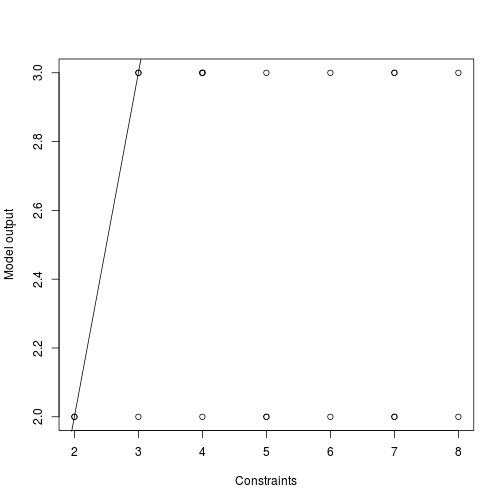
\includegraphics[width = 10cm]{unnamed-chunk-5}
 \end{center}
\caption[Scatter plot of the fit between census and survey data]
{Scatter plot of the fit between census and survey data. This plot
can be re-created using the plot command in listing \ref{cconv}.}
 \label{fct1}
\end{figure}

\begin{lstlisting}[float=h, caption={Reweighting of first constraint
and testing of results}, label=ccon1]
for (j in 1:nrow(all.msim)) {
 weights1[which(USd$age < 50),j] <- all.msim[j,1]/USd.agg[j,1]
 weights1[which(USd$age >= 50),j] <- all.msim[j,2]/USd.agg[j,2]
}
# Aggregate the results for each zone
for (i in 1:nrow(all.msim)) {
 USd.agg1[i,] <- colSums(USd.cat * weights0[,i] * weights1[,i])
}
# Test results
USd.agg1
##      16-49 50+     m     f
## [1,]     8   4 6.667 5.333
## [2,]     2   8 6.333 3.667
## [3,]     7   4 6.167 4.833
## [4,]     5   4 5.167 3.833
## [5,]     7   3 5.500 4.500

plot(as.vector(as.matrix(all.msim)),
 as.vector(as.matrix(USd.agg1)), xlab = "Constraints",
 ylab = "Model output")
abline(a = 0, b = 1)
\end{lstlisting}

\begin{figure}[h]
 \begin{center}
  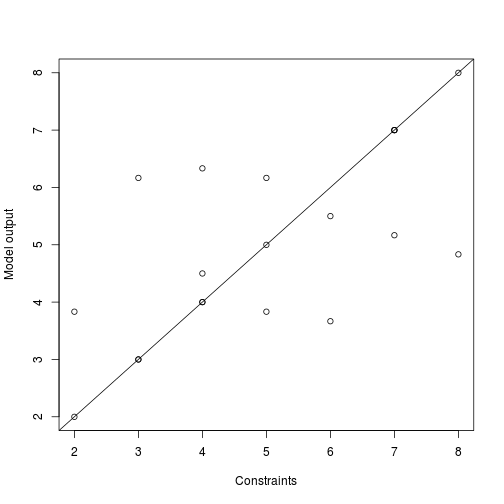
\includegraphics[width=10cm]{unnamed-chunk-6}
 \end{center}
\caption{Scatter plot showing the fit after constraining by age.} \label{fc1}
\end{figure}

We will perform the same checks after
each constraint to ensure our model is improving.
To see how the weights change for each individual for each area,
one simply types \verb weights1 , for constraint 1 (listing \ref{cmat}).
Note that the first column of weights 1 is the same as \cref{t:s}.
\begin{lstlisting}[caption = {The new weight matrix. Previously all weights were set to one.},
label =cmat]

##       [,1]  [,2]  [,3]  [,4] [,5]
## [1,] 1.333 2.667 1.333 1.333  1.0
## [2,] 1.333 2.667 1.333 1.333  1.0
## [3,] 4.000 1.000 3.500 2.500  3.5
## [4,] 1.333 2.667 1.333 1.333  1.0
## [5,] 4.000 1.000 3.500 2.500  3.5
\end{lstlisting}

To further improve the fit, one next constrains by the second aggregate constraint:
sex (listing \ref{con2}). To check that our implementation in R produces the
same results as the hand-calculated example, the resulting weights where queried.
As shown by \verb weights3[,1] , these are the same as
those calculated for $w(3)$ above.

\begin{lstlisting}[float=h, caption={Code to constrain the weights by
sex}, label=con2]
for (j in 1:nrow(all.msim)) {
    weights2[which(USd$sex == "m"),j] <-
		  all.msim[j,3]/USd.agg1[j,3]
    weights2[which(USd$sex == "f"),j] <-
		  all.msim[j,4]/USd.agg1[j,4]
}

weights3 <- weights0 * weights1 * weights2
for (i in 1:nrow(all.msim)) {
  USd.agg2[i,] <- colSums(USd.cat * weights3[,i])
}

weights3[,1]

## [1] 1.2 1.2 3.6 1.5 4.5
\end{lstlisting}

The model fit improves greatly after constraining for sex (r = 0.992).
However, to ensure perfect fit more iterations are needed. Iterating
just once more, as done on the online version of this
section\footnote{See
\href{http://rpubs.com/RobinLovelace/6193}{rpubs.com/RobinLovelace/6193}
}
results in a fit that is virtually perfect (\cref{fexits}). More iterations
are needed for larger datasets with more constraints to converge.

\begin{figure} \begin{center}
 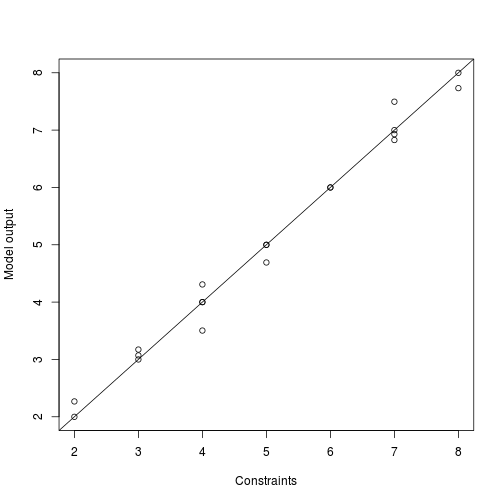
\includegraphics[width = 6cm]{unnamed-chunk-8}
 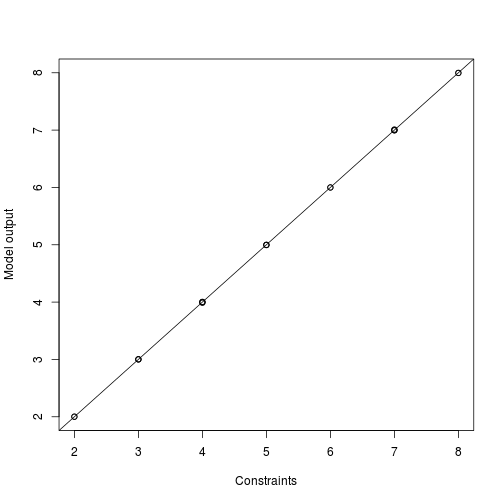
\includegraphics[width = 6cm]{unnamed-chunk-11}
 \end{center}
 \caption[Improvement of model fit with iterations]
 {Improvement of model fit after constraining by sex (left)
 and after two complete iterations (right).} \label{fexits}
\end{figure}

The worked code example in this section is replicable.
If all the code snippets are entered, in order, the results
should be the same on any computer running R. There
is great scope for taking the analysis further:
some further tests and plots are presented on the on-line
versions of this section. The simplest case is contained in
Rpubs document \href{http://rpubs.com/RobinLovelace/6193}{6193} and a more
complex case (with three constraints) can be found in Rpubs document
\href{http://rpubs.com/RobinLovelace/5089}{5089}. The preliminary checks
done on this code are important to ensure the model is understood
at all times and is working correctly. More systematic methods
for model checking are the topic of the following section.

\section{Model checking and validation} \label{smeval}

The R scripts that implement the methods described in \cref{setsim} and
\cref{s:integerisation} contain over 1000 lines of code.
This means that making mistakes while writing the code was almost inevitable,
from time to
time.\footnote{
A couple of examples serve to illustrate this point: during the construction of
vulnerability metrics based on the individual level output from the spatial
microsimulation model, the estimated expenditure on commuting was divided
by equivalised household income (a proxy of disposable income). 
One issue was that trip cost estimates are per year
while the income estimates are supplied per month in the USd. It took several
more alterations and runs of the model before the cause of the high proportion
of income spent on commuting (sometimes over 100\%) was realised. Another
example is simple typing errors while writing the code. The results are
presented in \cref{fig:error}, and are described below.
}
The large size of
the output files (approximately 250 Mb for 10 iterations of the spatial
microsimulation model for Yorkshire and the Humber) means that it would
be easy to miss fundamental errors. Hence the need for a
systematic strategy of checking the output. Beyond checking the model's
internal validity, it is necessary to test its external validity. This process,
validation, is inherently limited by lack of real spatial microdata.
Validation is a crucial step to take before the results are
presented, discussed and used as the basis of policy guidance. To make an
analogy with corporate food safety standards, it is important be open about and
highlight times when things do go wrong, in order to achieve high standards
\citep{Powell2011}. Transparency is needed in modelling for similar reasons
\citep{Tamminga2012}. This section is therefore an overview of the methods used
to find fault in the model, rather than assuming that everything is working
perfectly as the rest of the thesis does. It is divided into two halves: first
the process
of comparing the model results with knowledge of how it \emph{should}
perform \emph{a-priori} (model checking). Second, the
internally consistent model results are compared with external
empirical data (validation).
Validation is also discussed in the context of a single case study
in \cref{s:valid}.

\subsection{Model checking}
A proven method of checking that data analysis and processing is working
is wide ranging and continual visual exploration of its output
\citep{janert2010data}.
This strategy has been employed
throughout the modelling process, both to gain a better understanding of the
behaviour of the underlying R code, and to search for unexpected
results. These were often precursors to error identification.

An example of this, that illustrates the utility of ad-hock checks, is the
continual plotting of model inputs and outputs to ensure that they
make sense. The R commands \verb summary() \ and \verb plot() \ are ideal for
this purpose. The former provides basic descriptive statistics; the latter
produces a graphical display of the object. Both are \emph{polymorphic},
meaning that command adapts depending on the type of object it has been asked
to process \citep{Matloff-R}. Thus, to check that
the number of people in each age and sex category in the input and output
dataset made sense overall, the
following command was issued, resulting in the plot illustrated in \cref{fasp}:

\begin{lstlisting}
plot(cut(USd$age, breaks=(seq(0,100,20))), USd$sex)\end{lstlisting}
% TAKEN FROM ~/Dropbox/vul-meth/etsimY

\begin{figure}[h]
 \begin{center}
   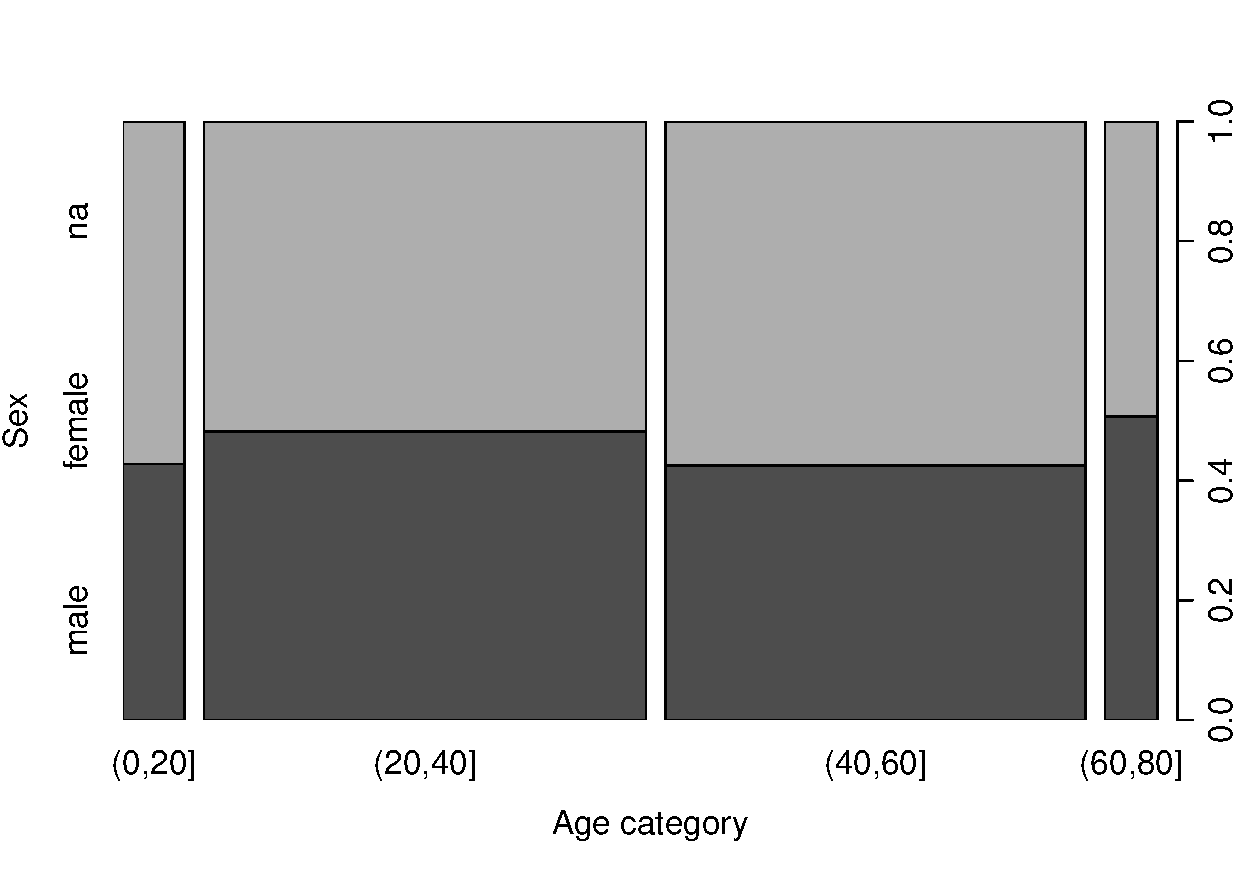
\includegraphics[width = 12cm]{age-sex-plot}
 \end{center}
 % cc-ems.pdf: 792x612 pixel, 72dpi, 27.94x21.59 cm, bb=0 0 792 612
\caption[Diagnostic plot to check the sanity of age and sex inputs.]{Diagnostic
plot to check the sanity of age and sex inputs. (Square brackets
indicate that the endpoint is not included in the set --- see
International Organization for Standardization
\href{http://www.iso.org/iso/catalogue_detail?csnumber=31887}{(ISO) 80000-2:2009},
formerly \href{http://en.wikipedia.org/wiki/Interval_(mathematics)}{ISO 31-11}
on ``mathematical signs and symbols for use in physical sciences and technology'').}
 \label{fasp}
\end{figure}
These common-sense methods of data checking may seem overly simplistic to warrant
mention. Yet such basic sanity tests are the `bread-and-butter' of
quantitative analysis. They ensure that the data are properly
understood \citep{Wickham2008}. Had the input data represented in \cref{fasp}
contained an equal proportion of people under 20 as over 20, for example,
one would know that the input data for commuters was faulty.
This approach, whereby major
problems are revealed early on in frequent tests, is preferable to waiting
until the results of the full spatial microsimulation are analysed. Hours were
saved, and understanding of the input datasets was improved.\footnote{The
use of the
same command to check model output was crucial to the identification of
important errors, including a small mistake in the code which led to large
errors in the synthetic microdata output for the distance constraint variables.}

The basic tenet of spatial microsimulation is that simulated and actual data
should match at the aggregate level \citep{Ballas2007simb}.
This knowledge led to the
continual plotting of census vs simulated results in the early stages of the
model construction, and the development of more
sophisticated plots (see \cref{fig:IPF-4c}).
Still, the humble scatter plot was used frequently for
preliminary analysis. To provide an example, after the model was run for
Yorkshire
and the Humber region for 20 iterations, I was confident the results were
correct: the results had been tested for Sheffield, and everything
\emph{seemed} to be working as expected.

Knowledge of how model-census fit should look started alarm bells
ringing when an imperfect plot was discovered:
% (largely by luck, as I was looking at the fit
% between only some of the variables, and happened to think the number of people
% taking very short trips could be subject to higher than normal levels of
% error). % What does this contribute? Nowt.
\cref{fig:error} (A) was cause for concern, not only for the low
correlation between the two variables (which was still greater than 0.8), but
because the direction of the error: the model had \emph{always} overestimated the
number of people travelling short distances to work in past runs.
This seemed suspicious, and the relationship was plotted for earlier constraints
to identify where the problem was variables were plotted.
\cref{fig:error} (B) was the
result of this, after constraining by distance.
Something had clearly gone wrong because no people who work
from home had been registered in the aggregate output. These issues led to
a re-examination of the code contained
within the file cats.r. It was found that a faulty placement of an
equals sign (such that values ``greater than or equal'' to 0 were accepted as 0
- 2 km travel to work). The problem was solved, and the model correlation
improved as a result (\cref{fig:error} (C)).

The two examples described above provided insight into how the model was
performing by its own standards. The more challenging stage is to validate
the model against factors external to it. % This is further discussed !!!

\begin{figure}[h]
  \begin{center}
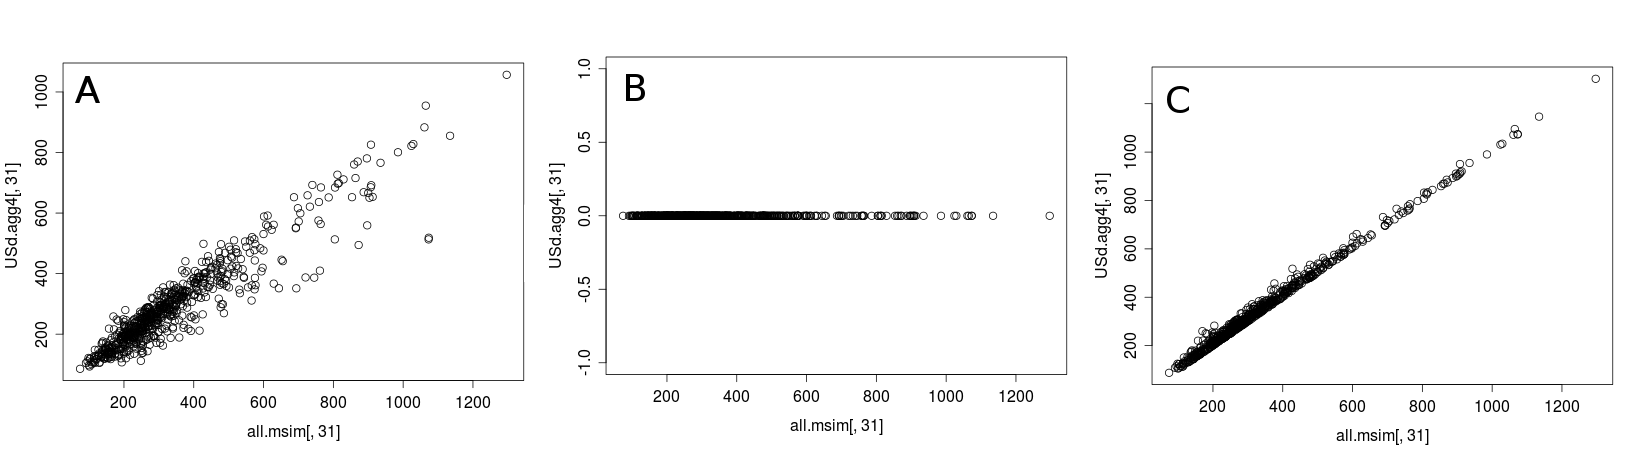
\includegraphics[width=15cm]{errors3-1}      \end{center}
 % cc-trans.png: 1113x529 pixel, 72dpi, 39.26x18.66 cm, bb=0 0 1113 529
 \caption[Diagnostic plots to identify model error]{Three diagnostic plots used
to identify a code error in the spatial microsimulation model (for the
distance category `travels 0--2 km to work'). The x-axis is
census data, the y-axis is the simulated result. A) First plot
analysed (for iteration 20); B) second plot, which illustrated the source of the
problem, in the distance constraint; C) satisfactory diagnostic plot,
after the problem had been resolved.}
 \label{fig:error}
\end{figure}

\subsection{Model validation}
\label{meval}
% {\color{red} Should this section be in a later chapter?} !!!
Beyond `typos' or simple conceptual errors in model code, more fundamental
questions should be asked of spatial microsimulation models. The validity
of the assumptions on which they are built, and the confidence one should have
in the results are important. This is especially true of models designed to inform
policies which have the potential to influence quality of life. Yet
evaluation and `validation' are
 problematic for any models that attempt to explain extensive, complex
systems such as cities or ecosystems. The urban modelling approach, of which
spatial microsimulation of commuters is a subset, has been grappling with this
problem since its infancy. Lacking a crystal ball, time-machine or settlements
on which controlled experiments can be performed, the difficulty of model evaluation can
seem intractable: ``only through time can a model be verified in any
conventional sense of the word'', by comparing the range of projected futures
with the reality of future change in hindsight \citep[p.~15]{batty1976urban}.

Why do urban models pose such a problem? Previously unknown knock-on impacts
cannot be ruled out due to the vast number of links between system
elements.\footnote{It is, of course, impossible to know how every resident of
an area interacts with every other, let alone predict the future impacts of
this interaction, even in the era of ubiquitous digital communications.
}
Rigorous real-world testing is usually impossible due to the scale of the system
and ethics involved with intervening in peoples' lives for the sake of research.
Controlled experiments cannot be performed on real settlements in the
same way that experiments can be performed in the physical sciences and, even if
two similar settlements could be found on which to apply different
interventions, there is no guarantee that all other factors will be held
constant throughout the duration of the experiment. %%% Refs!!!
% Going off on a bit of a waffle to be fair

Additional evaluation problems apply to spatial microsimulation models in
particular for a number of reasons, including:
\begin{itemize}
 \item The aggregate values of categorical `small area' constraint variables are already known from the Census, 
 so should be accurate. Checking the distribution of continuous variables such as 
 age and distance travelled to work against these crude categories is 
 problematic.\footnote{For example, if 50\% of
commuters in a particular area travel 2--5 km to work according to the Census,
does that mean that there is a normal distribution of trip distances with the
mean focussed on 3.5? Or is it more likely that there is a single large
employer located somewhere between 2 and 5 km from the bulk of houses in the
area, which accounts for the majority of these jobs and leads to a skewed
distribution of home-work distances. In every event, spatial microsimulation
will ignore such subtleties and smooth out extreme skewness by approximating the
national distance trends within each distance bin.
}
  \item Target variables are not generally known as geographic
aggregates. Therefore checking their validity for small areas is 
difficult: new surveys may be needed.
  \item Spatial microsimulation results in long lists of individuals for each
zone. With thousands of individuals in each zone and hundreds of zones, the
datasets can become large and unwieldy.
\end{itemize}

Regarding the target variables, inaccuracies can be expected because they are
determined entirely by their relationships with constraint variables. Also
it can be expected these relationships will not remain constant for all places:
perhaps in one area the number of female drivers is positively correlated to
distance travelled to work, yet there may be a different strength of
correlation, or the variables may be unrelated in another.

As mentioned above, validation of target variables is especially problematic
due to lack of data. To overcome this problem, two techniques were employed.
First, the interaction between constrained variables and unconstrained
variables was tested using data from the Census. Second, an additional dataset
from the UK's National On-line Manpower Information System
(Nomis) was harnessed to investigate the
correlation between unconstrained `interaction' variables --- those
composed of two or more constraint variables such as `female driver'.

The first approach tested the model's ability to simulate income. Although
income data are lacking for small areas, Neighbourhood Statistics
provides estimates of net and gross household incomes at the MSOA level. For the purposes of
this study, equivalised net income was used. The fit between the Neighbourhood
Statistics and simulated values are displayed in \cref{fig:income-test}.

\begin{figure}[h]
 \centering
 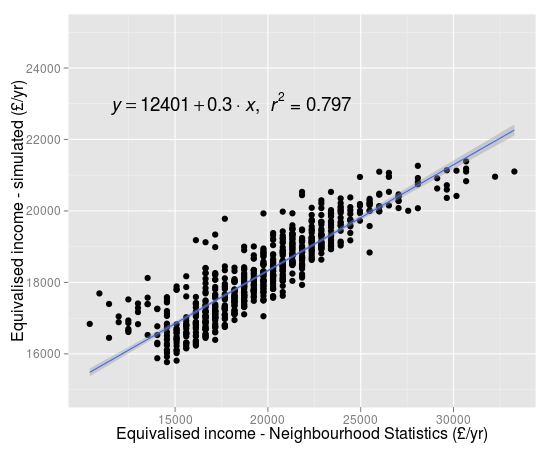
\includegraphics[width=12cm]{Income-check-morevars}
\caption[Scatter plot of simulated vs official estimated income]{Scatter plot
illustrating the correlation between mean
income simulated from the model and official estimates at the MSOA
leve.}
 \label{fig:income-test}
\end{figure}

The results show the microsimulation model could be used to predict income
(modelled income), accounting for almost 80\% of the variation in the
Neighbourhood Statistics data using an ordinary least squares (OLS) regression
model.
This is impressive, given that the aim of the model is not to simulate
income but energy costs of work travel, based on mode, distance, age/sex
and class. Of these socio-economic class is the only constraint
variable traditionally thought to be closely associated with income.
The main problem with the income estimates generated through spatial
microsimulation is the small range of estimates simulated:
the standard deviation was
\pounds1,194 and \pounds3,596 for the simulated and National Statistics data
respectively. (Note the
differences in the x and y axis scales in \cref{fig:income-test}.)
This underestimation of variance can be explained because social class,
distance and modes of transport are not sufficient to determine the true
variability in household incomes. Constraining by car ownership and tenure
variables would be likely to improve the fit.

The purpose of this fitting exercise is not so much to provide accurate income
estimates at the local level but to evaluate the
performance of the spatial microsimulation model. In terms of income, a variable
that is unconstrained in the model yet available from the survey data, the
spatial microsimulation model has worked well. The results suggest that the
values of unconstrained variables will not simply repeat the national average
for every small area, but will vary based on how their variation at the
national level is related to the constraint variables. In this case, the
assumption that the relationships between the target variable (income) and
constraint variables at the local level (in Yorkshire and the Humber) are
similar to the relationships between these variables at the national level,
receives support. How well does the model simulate other target variables such
as environmental habits, domestic energy use and levels of deprivation?
These are interesting
questions that merit further attention based on available data.

The second approach relies on Nomis, which provides cross-tabulations of census
variables, for example transport mode by class. The downside is that the data
are randomised, as stated at the bottom of each of their small-area census
tables: ``Figures have been randomly adjusted to avoid the release of
confidential data'' (this phrase appears in many of Nomis's tables.
One example can be found here:
\href{http://www.nomisweb.co.uk/livelinks/4652.xls}{http://www.nomisweb.co.uk/livelinks/4652.xls}).

In order to harness Nomis data to test the accuracy of the microsimulation
model for calculating, it was first necessary to establish how accurate Nomis
data are. How much have Nomis data been randomised, and in what way? 
This question is relatively easy to 
answer because of the census variables shared between those published 
by Nomis and by Casweb at the MSOA level. Scatter plots
suggest Nomis data are faithful to the original census results:

\begin{figure}[h]
 \centering
 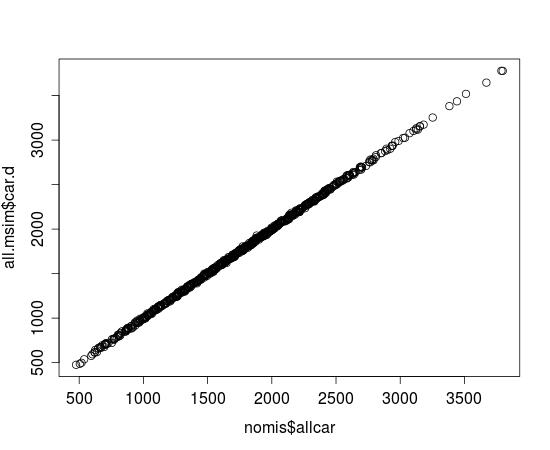
\includegraphics[width=6.6cm]{nomis-vs-cens-car}
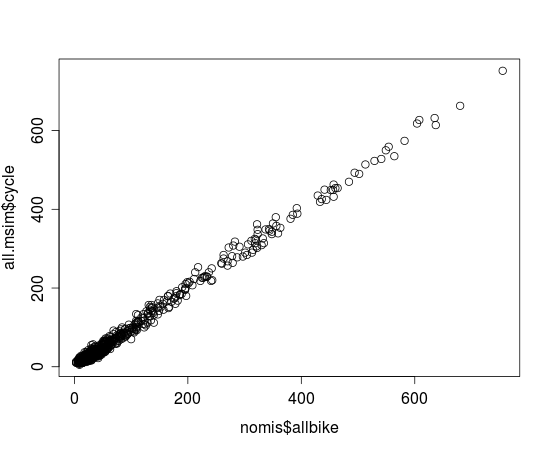
\includegraphics[width=6.6cm]{nomis-vs-cens-bike}
 % Graph-line.pdf: 516x363 pixel, 72dpi, 18.20x12.81 cm, bb=0 0 516 363
 \caption[Scatter plot of error introduced in Nomis data]{Scatter graphs
illustrating the fit between Nomis
and Casweb versions of the same census variables. The correlation (Pearson's r)
is 0.9998 and 0.9969, for the number of car drivers and number of cyclists in
each MSOA respectively.}
 \label{fig:nomis-vs-cens-car}
\end{figure}

From \cref{fig:nomis-vs-cens-car} it is interesting to note that the
correlation decreases for cyclists. This, it was inferred, could represent
an increase in the signal-to-noise ratio for variables with small values
to a fixed randomising factor.  To test this, the errors were plotted for
variables with large (car drivers) and small (cyclists) totals. The results
indicate that the noise added by randomisation is equal for each variable,
regardless of the cell count (\cref{fig:nomis-ers}).

 \begin{figure}[h]
 \centering
 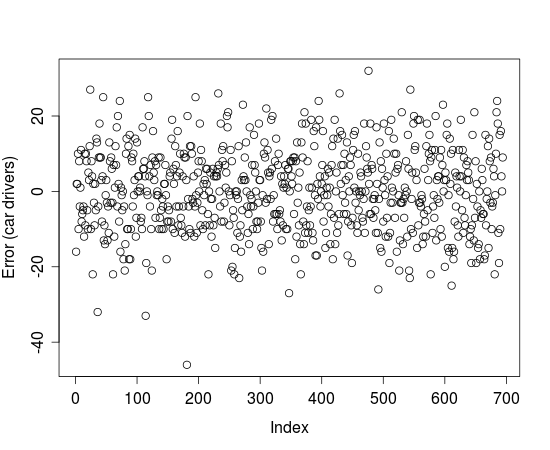
\includegraphics[width=6.6cm]{car-ers}
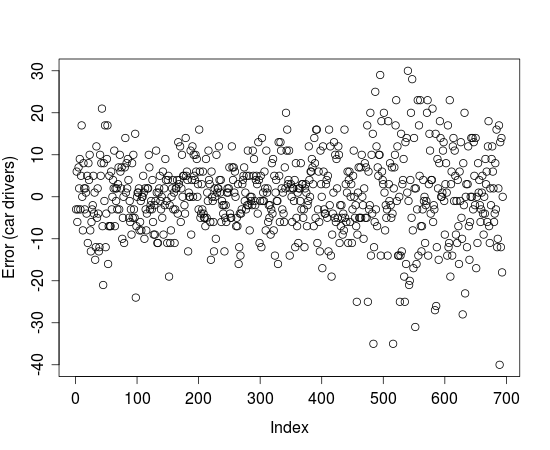
\includegraphics[width=6.6cm]{bike-ers}
 % Graph-line.pdf: 516x363 pixel, 72dpi, 18.20x12.81 cm, bb=0 0 516 363
 \caption[Errors associated with Casweb census variables]
{Errors (Casweb values -- Nomis values) associated with car driver
(right) and bicycle commuter (left) census variables.}
 \label{fig:nomis-ers}
\end{figure}

The errors seem to be similar, with a range of approximately 70 and a mean of
zero. This observation is confirmed by descriptive statistics for each set of
errors (standard deviation = 11.01, 9.47; mean = 0.15, 0.23) for car driver and
cyclist variables respectively. We can therefore conclude that the error added
by randomisation is constant for each variable and this was confirmed by plotting
the errors for additional census variables. Q-Q plots --- which compare the 
quantile values of one distribution against another, in this case those of 
the errors against those of the normal distribution --- suggest that the
distribution of error is approximately normal.

These exploratory methods provide confidence in the Nomis data, but only for
relatively large cell counts (the signal-noise ratio approaches 1:1 as the cell
count approaches 20): therefore evaluations based on Nomis data are better
suited to cross tabulated categories that have high cell counts, for example car
drivers. In our microsimulation model, both gender and mode of
transport are constrained, but not simultaneously, so the fit between the Nomis
cross-tabulation and the cross-tabulation resulting from our model provides
some indication of accuracy. The results are presented in
\cref{no-vs-sim-mcar}. Interestingly, the accuracy of this `partially
constrained' simulated target variable appears to be worse than that of the
completely unconstrained income variable (compare \cref{no-vs-sim-mcar}
and \cref{fig:income-test}). In both cases, the correlation is reasonably strong
and positive (0.47 and 0.80 respectively). However, as with the income
estimates, the \emph{distribution} of estimates arising from the model
is less dispersed than actual data: the standard deviation for the former (0.30)
is substantially less than for the latter (0.44). This illustrates the tendency
of spatial microsimulation models to underestimate the extent of spatial
variation. %%% citep{} ???

\begin{figure}
 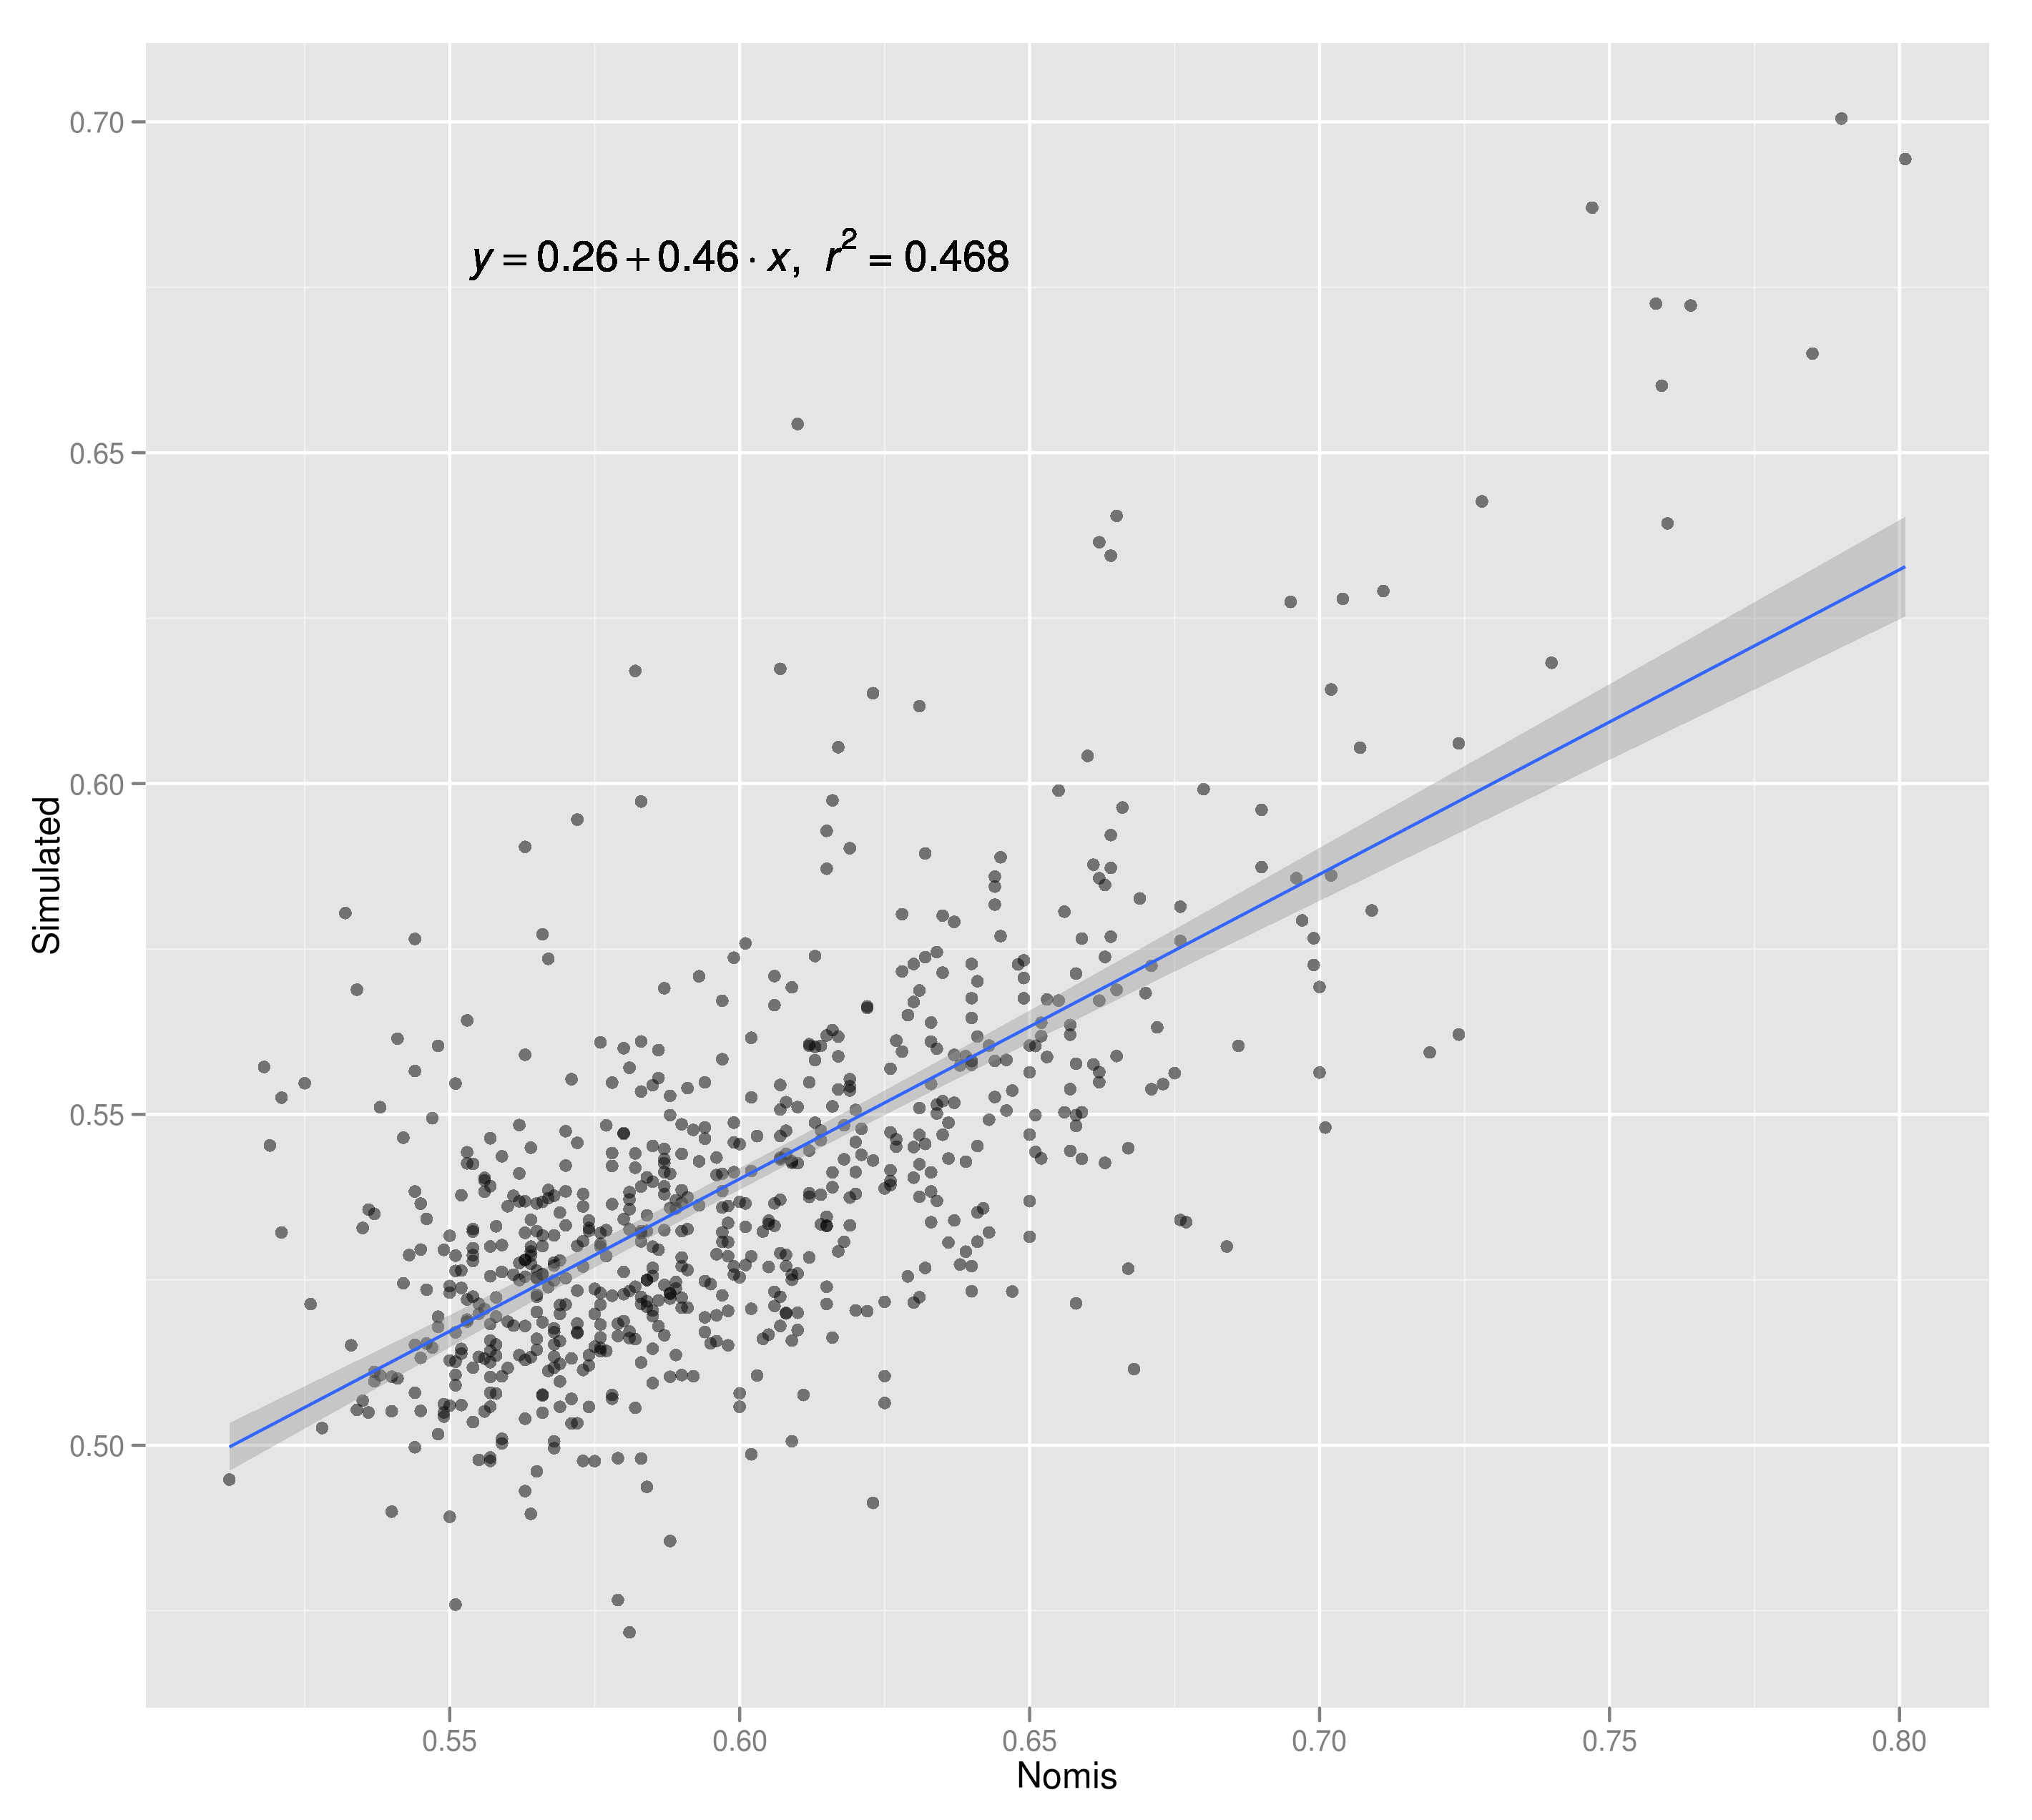
\includegraphics[width = 12 cm]{no-vs-sim-mcar}
\caption[Scatter plot of the proportion of male drivers]{Scatter plot of
the proportion of male drivers in each MSOA area in
Yorkshire and the Humber according to simulated and Nomis data.}
\label{no-vs-sim-mcar}
\end{figure}

\subsection{Additional validation methods}
The methods described above illustrate the techniques used to prevent
model errors and ensure that the results were compatible with external data
sources. But they only scratch the surface of what is possible in terms of
model validation. This section will not go into detail. Its
purpose is to draw attention to
additional methods that could be conducted as lines of future research
and discuss the merits of each. Specifically, the following additional validation
methods could (given sufficient resources) be implemented:
\begin{itemize}
 \item Primary data collection of target variables at the individual level
 in specific areas to  validate the spatial microdata locally.
 \item Comparing of the spatial microdata over entire region with a
 survey data that specifies home region of resident.
 \item Aggregating local model outputs to coarser geographical levels at which
 cross-tabulated data are available.
 \item Comparison of mode and distance data with external correlates of personal
 travel (e.g.~MOT data on distance travelled and bus usage data).
\end{itemize}

Other than the sanity check of age-sex ratios presented in \cref{fasp},
the evaluation methods considered above operate at the level of geographically
aggregated counts. However, the unique feature of spatial microsimulation is
its simulation of individuals. Evaluation techniques should therefore operate
at the individual level as well.
% The potential for evaluation of the simulated
% spatial microdata outputs is limited by the availability of official spatial
% microdata. As a result this section is short and, for the most part,
% purely theoretical.
%
% The available datasets were introduced with reference to an idealised
% `perfect' dataset on commuting \cref{fdata-ideal}. In the same way, we will
% describe methods of evaluating the microsimulation model at the individual
% level with reference to the ideal of unlimited data. This will inform the
% discussion of how best to use the individual level data that is available
% for model evaluation...
Because simulation, almost by definition, estimates something that is not
otherwise known, it is hard to find reliable individual level
data against which the estimates can be evaluated. For this reason
individual level surveys could be conducted in a specific area where
spatial microdata have been generated. To take one example, a randomised
sample of households could be taken in a single ward. Respondents would be
asked the mode of travel to work, distance and frequency of trip and
other variables. This would allow the model to be evaluated
not only in terms of the correlations that it outputs between different categories,
but also for the evaluation of the assumptions on which the energy calculations %??? where
are based.

One of the main advantages %cited where???
of spatial microsimulation over just using aggregated data is that it provides
insight into the \emph{distribution} of continuous variables within each zone,
rather than just counts of categories which are often rather coarse. T-tests and
Analysis of Variance (ANOVA) tests could then be used to check if the
mean and variance of the simulated and survey data are statistically likely
to be from the same population. However, the raw results of IPF are not
conducive to such tests at the individual level because they do not contain
whole individuals. Integerisation of the weight matrices is needed.


\section{Integerisation} \index{integerisation}
\label{s:integerisation}
An important advantage of spatial microsimulation models is their ability
to model individuals. Yet, as shown in the previous section, the IPF
procedure does not result in whole individuals, but fractions of individuals.
This is not a problem if the aim of spatial microsimulation is \emph{small area
estimation} \citep{Ballas2005b}. However, the potential to model individual
people using agent-based modelling techniques can make spatial microsimulation
much more powerful. One way to tackle this issue is by using a different
reweighting strategy to select representative individuals for each area.
An alternative is to convert the results of IPF into
integer results. \citet{Lovelace2013-trs} tackled this issue in detail and
developed a new method of integerisation. The following section is therefore
based on \citet{Lovelace2013-trs} and repeats much of the content.

The aim of IPF, as with all spatial microsimulation methods, is to  match
individual level data from one source to aggregated data from another.
IPF does this repeatedly, using one constraint variable at a time: each
brings the column and row totals of the simulated dataset closer to
those of the area in question (see \citealp{Ballas2005b} and
Fig.~\ref{fig:IPF-4c} below).

Unlike combinatorial optimisation algorithms, IPF results in non-integer
weights. As mentioned above, this is problematic for certain applications.
In their overview of methods for spatial microsimulation
\citet{Williamson1998} favoured combinatorial
optimisation approaches, precisely for this reason:
%It should be noted that only integer reweighting schemes are to be considered
``as non-integer weights lead, upon tabulation of results, to fractions of
households or individuals'' (p.\ 791). There are two options
available for dealing with this problem with IPF:
\begin{itemize}
\item Use combinatorial optimisation microsimulation methods instead
\citep{Williamson1998}. However, this can be computationally intensive
\citep{Pritchard2012}.
\item Integerise the weights: Translate the non-integer weights obtained
through IPF into discrete counts of individuals selected from the original
survey dataset \citep{Ballas2005c}.
\end{itemize}
We revisit the second option, which arguably provides the
`best of both worlds': the simplicity and computational speed of deterministic
reweighting and the benefits of using whole individuals rather than fractions.
%allows for the
%use of simple IPF models to deterministically provide the best possible fit
%between
% As with any model, spatial microsimulation models are rough approximations
% of an infinitely complex reality and, as with any model, they rely on
% assumptions about how the world works. In this case the founding assumption is
% that the relationships between the constraint variables and the target
%variables
% are the same for individuals in the survey as for individuals in the
% areas under investigation. Using the example of income, its dependence on age
%is
% assumed to remain constant in each area. If young people earn less money in
%the
% survey, an area containing a high proportion of young people will be expected
%to
% have a low income relative to an area containing a low proportion of young
% people, all other factors being equal. The technique makes the assumption
% that relationships between socio-economic variables remain constant over space
% \citep{Cullinan2011}.
% composed of scattered points whose
%characteristics vary are ubiquitous in Geography,
%or `integer reweighting', as it also called \citep{Ballas2005},
%Examples of why integerisation is useful

IPF is an established method for combining microdata
with spatially aggregated constraints to simulate  target variables whose
characteristics are not recorded at the local level. Integerisation translates
the real number weights obtained by IPF into samples from the original
microdata, a list of `cloned' individuals for each simulated area.
Integerisation may also be useful conceptually, as it allows
researchers to deal with entire individuals. The next section
reviews existing strategies for integerisation.

\subsection{Method}
\label{strategies}
Despite the importance of integer weights for dynamic spatial microsimulation,
and the continued use of IPF, there
has been little work directed towards integerisation. It has been noted that
``the
integerization and the selection tasks may introduce a bias in the synthesized
population'' \citep[10]{Muller2010}, yet little work has been done to find out
\emph{how much} error is introduced.

To test each integerisation method, IPF was used to generate an
array of weights that fit individual level survey data to
geographically aggregated census data (see Section \ref{worked-eg}). Five
methods for
integerising the results are described, three deterministic and two
probabilistic. These are: `simple rounding', its evolution into the `threshold
approach' and the `counter-weight' method and the probabilistic methods:
`proportional probabilities' and `truncate, replicate, sample'. TRS
builds on the strengths of the other methods, hence the order in which they are
presented.

The application of these methods to the same dataset and their implementation in R allows
their respective performance characteristics to be quantified and compared.
Before proceeding to describe the mechanisms by which these integerisation
methods work, it is worth taking a step back, to consider the nature and
meaning of IPF weights.

\subsubsection{Interpreting IPF weights: replication and probability}
It is important to clarify what is meant by `weights' before proceeding to
implement methods of integerisation: this understanding was central to the
development of the integerisation method presented in this section.
The weights obtained through IPF are real numbers ranging from 0 to hundreds
(the largest weight in the case study dataset is 311.8). This range
makes integerisation problematic: if the probability of selection is
proportional to the IPF weights, as is the case with the `proportional
probabilities' method,
the majority of resulting selection probabilities can be very low.
This is why the simple rounding method rounds weights up or down to the nearest
integer weight to determine how many times each individual should be
replicated (Ballas et al., 2005a). This ensures that replication weights do not differ
greatly from non-integer IPF weights. However, some of the information contained
in the weight is lost during rounding: a weight remainder of 0.501 is treated
the same as 0.999.

This raises the following question: Do the weights refer to the number of times
a particular individual should be replicated, or is it related to the
probability of being selected? The following sections
consider different approaches to addressing this question, and the
integerisation methods that result.


IPF weights do not merely represent the probability of a single case
being selected. They also (when above one) contain information about
repetition: the two types of weight are bound up in a single number. An
IPF weight of 9, for example, means that the individual should be replicated
9 times in the synthetic microdataset. A weight of 0.2, by contrast, means
that the characteristics of this individual should count for only 1/5 of their
whole value in the microsimulated dataset and that, in a representative
sampling strategy, the individual would have a probability of 0.2 of being
selected. Clearly, these are very different concepts. As such, the TRS approach
to integerisation isolates
the replication and probability components of IPF weights at the outset, and
then deals with each separately. Simple rounding, by contrast, interprets IPF
weights as inaccurate count data.


\subsubsection{Simple rounding}
The simplest approach to integerisation is to convert the non-integer
weights into an integer by rounding up if 
the decimal is 0.5 or above or down otherwise.
Rounding alone is inadequate for accurate results, however. As illustrated in
Fig.~\ref{fig:histws} below, the distribution of weights obtained by IPF is
likely to be skewed, and the majority of weights may fall below the critical 0.5
value and be excluded. As reported by \citet[25]{Ballas2005c}, this results in
inaccurate total populations. To overcome this problem
\citet{Ballas2005c} developed algorithms to `top up' the simulated
spatial microdata with
representative individuals: the `threshold' and `counter-weight' approaches.

\subsubsection{The threshold approach}
\citet{Ballas2005c} tackled the need to `top up' the simulated area
populations such that $Pop_{sim} \geq Pop_{cens}$. This is done by creating an inclusion
threshold ($IT$) set to 1 which iteratively
reduced. This samples additional individuals with
incrementally lower weights.\footnote{A 
more detailed description of the steps
taken and the R code needed to perform them iteratively can be found in the
Supplementary Information, Section 3.2.}
Below the exit value of $IT$ for each zone, no individuals can be included
(hence the clear cut-off point around 0.4 in Fig.~\ref{fig:threshweights}).
In its original form, based on rounded weights, this approach over-replicates
individuals with high decimal weights.
To overcome this problem, the truncated weights were taken as the starting
population, rather than the rounded weights. This modified approach improved the
accuracy of the integer results and is therefore the meaning of
the `threshold approach' henceforth.\footnote{An
explanation of this improvement can be illustrated by considering an individual
with a weight of 2.99. Under the original threshold approach described by
\citet{Ballas2005c}, this person would be replicated 4 times: three times after
rounding, and then a
fourth time after $IT$ drops below 0.99. With our modified approach they would
be replicated three times: twice after truncation, and again after $IT$ drops
below 0.99. The improvement in accuracy in our tests was substantial, from a TAE
(total absolute error, described below) of 96,670 to 66,762. Because both
methods are equally easy to implement, only to the superior
version of the threshold integerisation
method is used.}

The technique successfully tops up integer populations yet has
a tendency to generate too many individuals for each zone.
This oversampling is due to duplicate weights --- each unique weight was
repeated on average 3 times in our model --- and the presence of
weights that \emph{are} different, but separated by less than 0.001.
(In our test, the mean number of unique weights falling into
non-empty bins between 0.3 and 0.48 in each area --- the range of values
reached by $IT$ before  $Pop_{sim} \geq Pop_{cens}$ --- is almost two.)


\subsubsection{The counter-weight approach}
An alternative method for topping-up integer results arrived at by simple
rounding was also described by \citet{Ballas2005c}. The approach was labelled
to emphasise its reliance on both counter and a weight variables. Each
individual is first allocated a counter in ascending order of its IPF weight.
The algorithm then tops-up the integer results of simple rounding by iterating
over all individuals in the order of their count. With each iteration the new
integer weight is set as the rounded weight plus the rounded sum of its decimal
weight plus the decimal weight of the next individual, until the desired total
population is reached.\footnote{This process is described in more detail in the
Supplementary Information.} %%% Now do it!

There are two theoretical advantages of this approach: its more accurate
final populations (it does not automatically duplicate individuals with equal
weights as the threshold approach does) and the fact that
individuals with decimal weights down to 0.25 may be selected.
This latter advantage is minor, as $IT$ reached below 0.4 in many cases
(Supplementary Information, Fig.~2) --- not far off.
A band of low weights (just above 0.25)
selected by the counter-weight method can be seen in
Fig.~\ref{fig:threshweights}.

The total omission of weights below some threshold is problematic for all
deterministic algorithms tested here: they imply that someone with a weight
below this threshold, for example 0.199 in our tests, has the same sampling
probability as someone with a weight of 0.001: zero! The complete
omission of low weights fails to make use of all the information stored in
IPF weights: in fact, the individual with an
IPF weight of 0.199 is 199 times more representative of the area (in terms of
the constraint variables and the make-up of the survey dataset) than the
individual with an IPF weight of 0.001. Probabilistic approaches to
integerisation ensure that all such differences between decimal weights
are accounted for.

\begin{figure}[t]
 \centerline{ 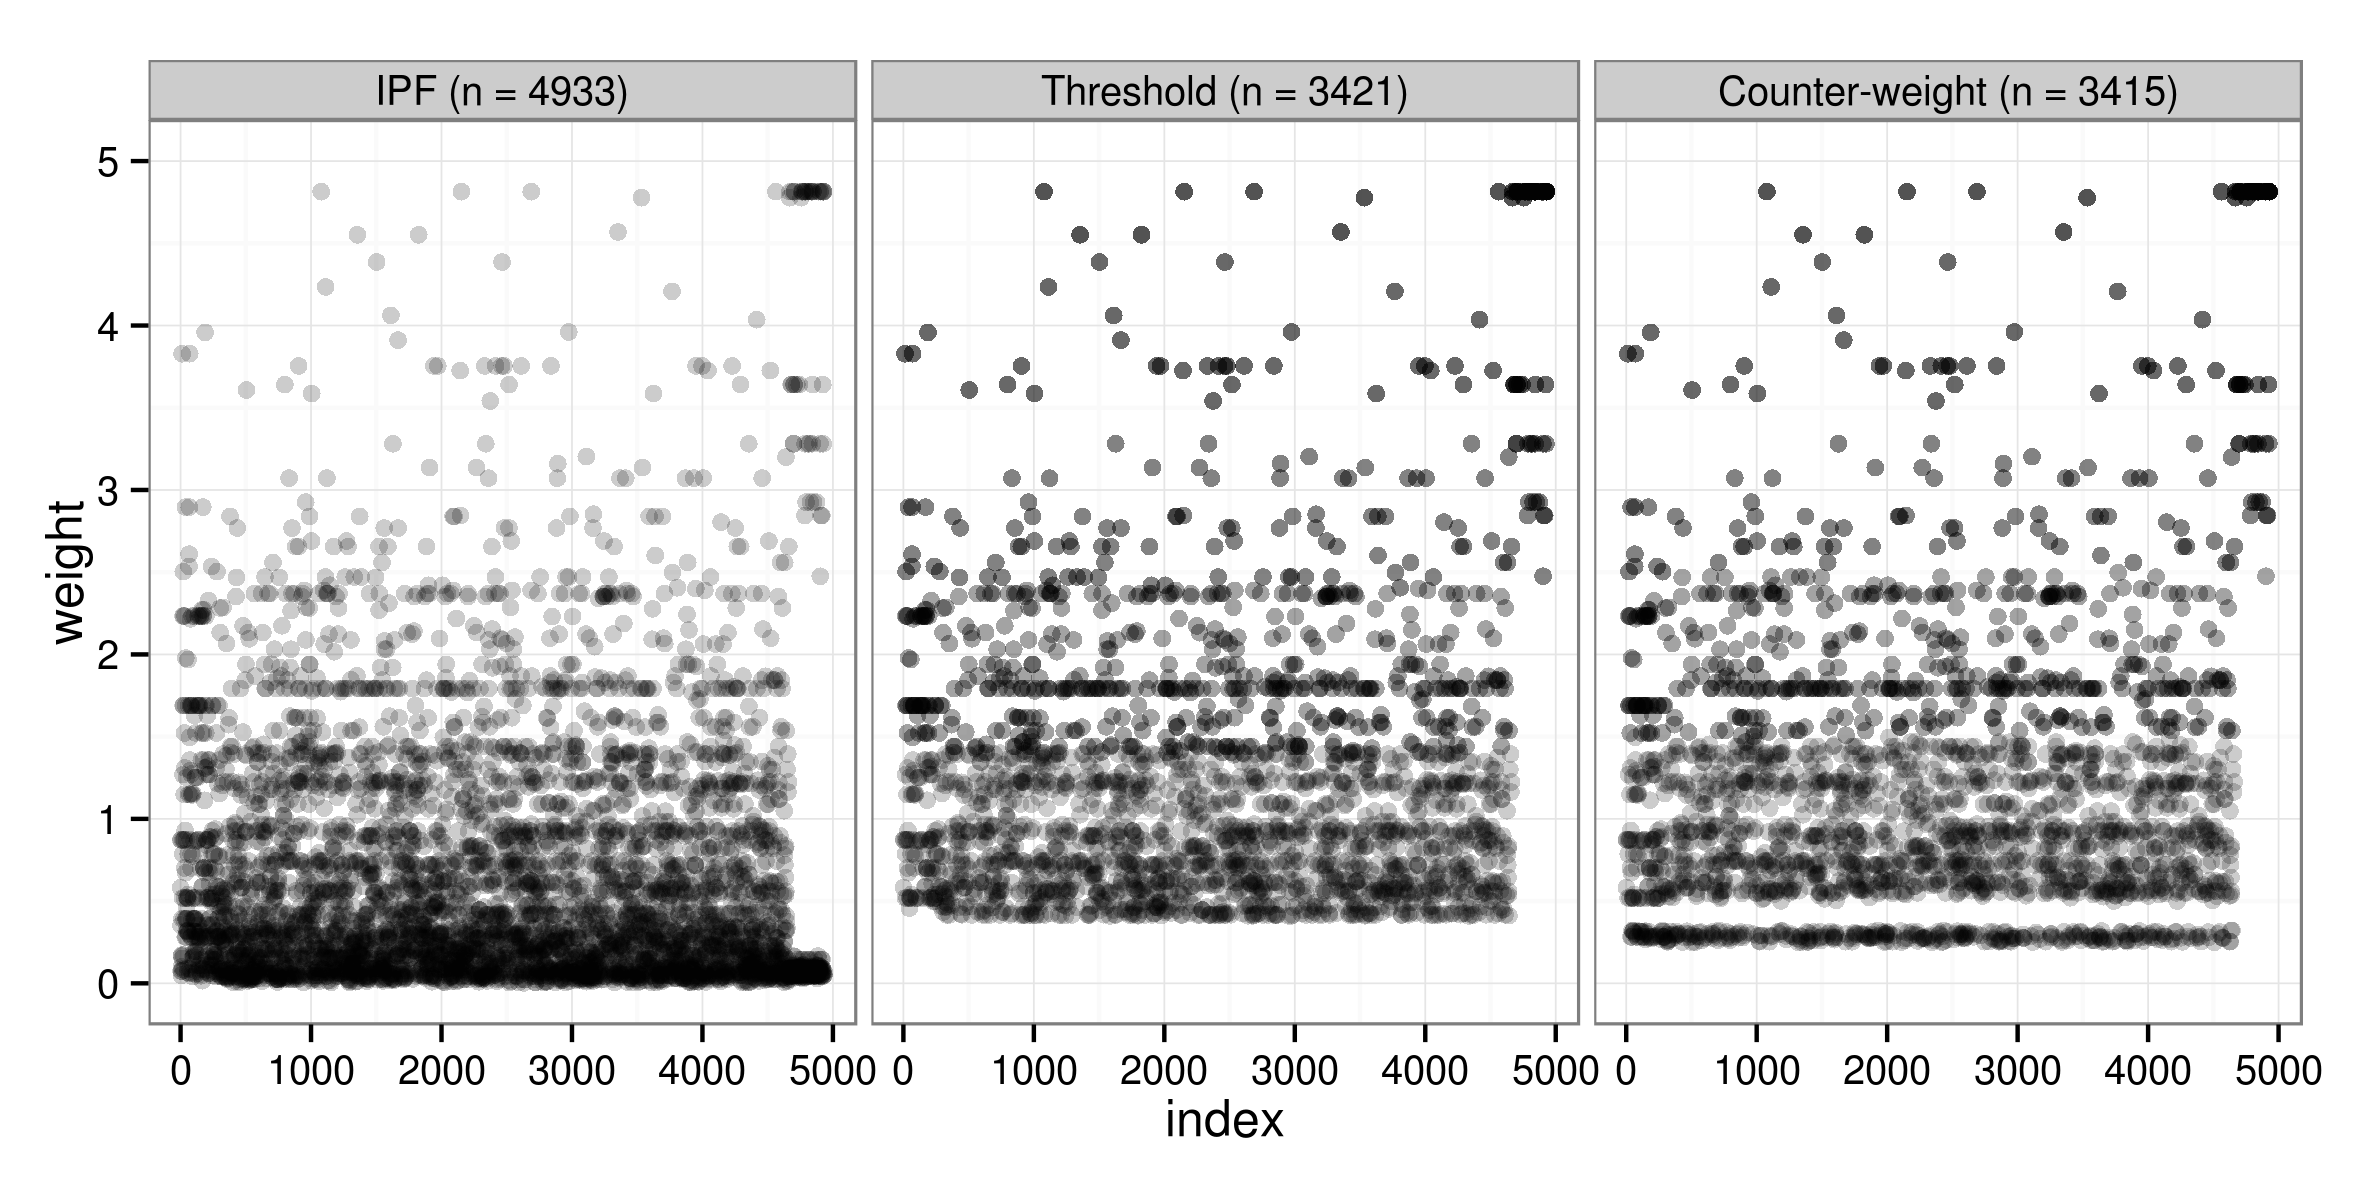
\includegraphics[width=14 cm]{IvW3}}
 % meths-scat.pdf: 792x612 pixel, 72dpi, 27.94x21.59 cm, bb=
 \caption[Overplotted scatter graph showing the distribution of IPF
weights]{Overplotted scatter graph showing the distribution of weights and
replications after IPF in the original survey (left), those selected
by inclusion thresholds for a single area (middle), and those selected
by the counter-weight method (right) for zone 71 in the
example dataset. The lightest points represent individuals who have been
replicated once, the darkest 5 times.}
 \label{fig:threshweights}
\end{figure}

% \begin{figure}[t]
%  \centerline{ 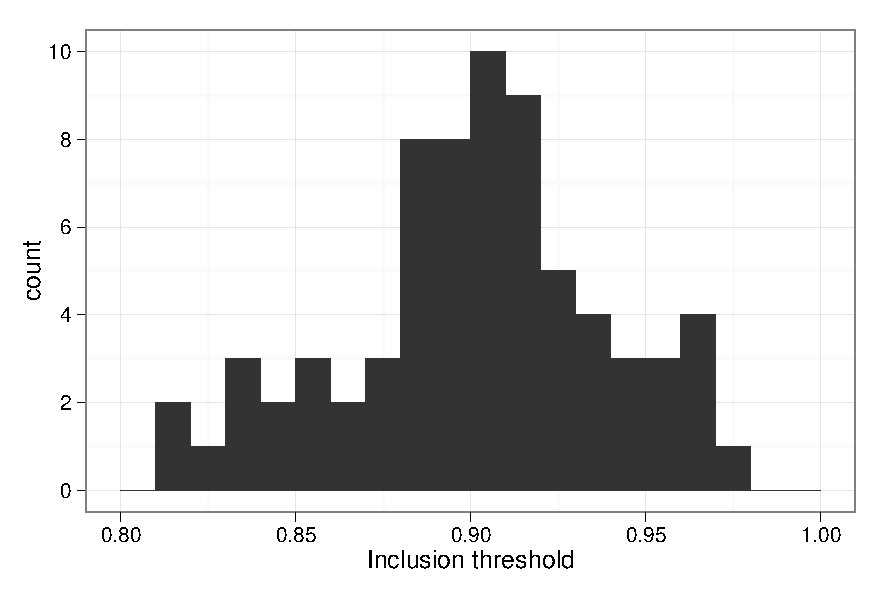
\includegraphics[width=14 cm]{Inclusion-hist2.pdf}}
%  % meths-scat.pdf: 792x612 pixel, 72dpi, 27.94x21.59 cm, bb=
%  \caption{Histogram of the inclusion thresholds ($IT$) reached in order
% to `top-up' individuals selected by simple rounding. (n = 71 zones.)}
%  \label{fig:Inclusion-hist}
% \end{figure}

\subsubsection{The proportional probabilities approach}
This approach to integerisation treats IPF weights as probabilities.
The chance of an individual being selected is proportional to the IPF
weight:
\begin{equation}
 p = \frac{w}{\sum{W}}
\end{equation}
Sampling until $Pop_{sim} = Pop_{cens}$ \emph{with replication} ensures that
individuals with high weights are likely to be repeated several times
whereas individuals with low weights are unlikely to appear.
% Due to the law of rare events, the probability that an individual with
% weight $w$ will appear  $X \in \mathbb{N}$ times in the integerised results
% follows
% the Poisson distribution:
% \begin{equation}
% p\left( X \right) = \frac{{e^{ - w } w ^X }}{{X!}}
% \end{equation}
The outcome of this strategy is correct from a theoretical perspective,
yet because all weights are treated as
probabilities, there is a non-zero
chance that an individual with a low weight
(e.g.~0.3) is replicated
more times than an individual with a higher weight (e.g.~3.3). (In this
case the probability for any given area is $\sim$ 1\%, regardless of the
population size). Ideally, this should never happen: the individual with weight
0.3 should be replicated either 0 or 1 times, the probability of the latter
being 0.3. The approach described in the next section addresses these issues.

\subsubsection{Truncate, replicate, sample}
\label{s:trs}
The problems associated with the aforementioned integerisation strategies
demonstrate the need for an alternative method.
Ideally, the method would build upon the simplicity of the
rounding method, select the correct simulated population size (as attempted by
the threshold approach and achieved by using `proportional probabilities'),
make use of all the information stored in IPF
weights \emph{and} reduce the error introduced by integerisation to a
minimum. The probabilistic approach used in `proportional probabilities'
allows multiple answers to be calculated (by using different `seeds').
This is advantageous for analysis of uncertainty introduced by the
process and allows for the selection of the best fitting result.
Consideration of these design criteria led us to
develop TRS integerisation, which interprets weights as
follows: IPF weights do
not merely represent the probability of a single case being selected. They
also (when above one) contain information about repetition: the two
types of weight are bound up in a single number. An IPF weight of 9, for
example, means that the individual should be replicated 9 times in the
synthetic microdataset. A weight of 0.2, by contrast, means that the
characteristics of this individual should count for only 1/5 of their whole
value in the microsimulated dataset and that, in a representative
sampling strategy, the individual would have a probability of 0.2 of
being selected. Clearly, these are different concepts. As such, the
TRS approach to integerisation isolates the replication and probability
components of IPF weights at the outset, and then deals with each separately.
Simple rounding, by contrast, interprets IPF weights as inaccurate count data.
The steps followed by the TRS approach are  described in detail below.

\emph{Truncate}

By removing all information to the right of the decimal point, truncation
results in integer values --- integer replication weights that
determine how many times each individual should be `cloned' and placed into the
simulated microdataset. In R, the following command is used: \begin{verbatim}
count <- trunc(w)
\end{verbatim}
% This command is identical to integer division by 1 \begin{verbatim}
% x %/% 1
% \end{verbatim},
where \verb w \ is a matrix of individual weights.  Saving these values (as
\verb count ) will later ensure  that only whole integers are counted. The
decimal remainders (\verb dr ), which vary between 0 and 1, are saved by
subtracting the integer weights from the full weights:\begin{verbatim}
dr <- w - count
\end{verbatim}
This separation of conventional and replication weights provides the
basis for the next stage: replication of the integer weights.

\emph{Replicate}

In spreadsheets, replication refers simply to copying cells of
data and pasting them elsewhere. In spatial microsimulation, the
concept is no different. The number of times a
row of data is replicated depends on the integer weight: an IPF
weight of 0.99, for example, would not be replicated at this stage
because the integer weight (obtained through truncation) is 0.

To reduce the computational requirements of this stage, it is best
to simply replicate the row number (\verb index ) associated with
each individual, rather than replicate the entire row of data. This
is illustrated in the following code example, which appears
within a loop for each area (\verb i ) to be simulated:
\begin{verbatim}
 ints[[i]] <- index[rep(1:nrow(index),count)]
\end{verbatim}

Here, the indices (of weights above 1, \verb index ) are selected
and then repeated. This is done using the function \verb rep() .
The first argument (\verb 1:nrow(index) ) simply defines
the indices to be replicated; the second (\verb count )
refers to the integer weights defined in the previous subsection.
(Note: \verb count \ in this context refers only to the
integer weights above 1 in each area).
 Once the replicated indices have been generated, they
can then be used to look up the relevant characteristics of
the individuals in question.

\begin{figure}[h]
 \centerline{ 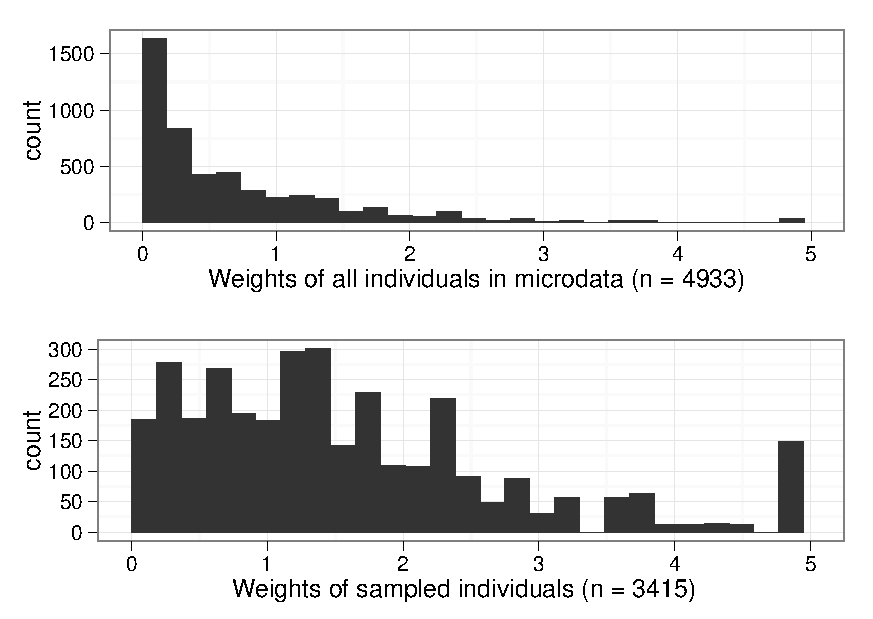
\includegraphics[width=14 cm]{hist-weights2.pdf}}
 % hist-weights.pdf: 792x612 pixel, 72dpi, 27.94x21.59 cm, bb=0 0 792 612
 \caption[Histograms of original microdata and integerised weights]{Histograms
of original microdata weights (above) and sampled microdata after TRS
integerisation (below) for a single area --- zone 71 in the case study data.}
 \label{fig:histws}
\end{figure}

\emph{Sample}

As with the rounding approach, the truncation and replication stages alone
are unable to produce microsimulated datasets of the correct size. The problem
is exacerbated by the use of truncation instead of rounding: truncation is
guaranteed to produce integer microdataset populations
that are smaller, and in some cases much smaller than the actual (census)
populations. In our case study,
the simulated microdataset populations were around half the
actual size populations defined by the census. This under-selection of
whole cases has the following advantage: when using truncation there
is no chance of over-sampling, avoiding the problem of
simulated populations being slightly too large, as can occur
with the threshold approach.

Given that the replication weights have already been included in steps 1 and 2,
only the decimal weight remainders need to be included. This can be done using
weighted random sampling without replacement. In R, the following function is
used:
\begin{verbatim}
  sample(w, size=(pops[i,1] - pops[i,2]), prob= dr[,i])
\end{verbatim}
Here, the argument \verb size \ within the \verb sample \ command is set as the
difference between the known population of each area (\verb pops[i,1] ) and
the size obtained through the replication stage alone (\verb pops[i,2] ). The
probability (\verb prob ) of an individual being sampled is determined by the
decimal remainders. \verb dr \ varies between 0 and 1, as described above.

The results for one particular area are presented in Fig.~\ref{fig:histws}.
The distribution of selected individuals has shifted to the right, as
the replication stage has replicated individuals as a function of their
truncated
weight. Individuals with low weights (below one) still constitute a large
portion of those selected, yet these individuals are replicated fewer times.
After TRS integerisation individuals with high decimal weights are relatively
common. Before integerisation, individuals with IPF weights between 0 and 0.3
dominated. An individual-by-individual visualisation of the Monte Carlo
sampling strategy is provided in Fig.~\ref{fig:index-weight-TRS}. Comparing
this with the same plot for the probabilistic methods
(Fig.~\ref{fig:threshweights}), the most noticeable difference is that the TRS
and proportional probabilities approaches
include individuals with very low weights. Another important difference is
average point
density, as illustrated by the transparency of the dots: in
Fig.~\ref{fig:threshweights}, there are shifts near the decimal
weight threshold ($\sim$ 0.4 in this area) on the y-axis.
In Fig.~\ref{fig:index-weight-TRS}, by contrast, the transition is
smoother: average darkness of single dots (the number of replications)
gradually increases from 0 to 5 in both probabilistic methods.

\begin{figure}[h]
 \centerline{
 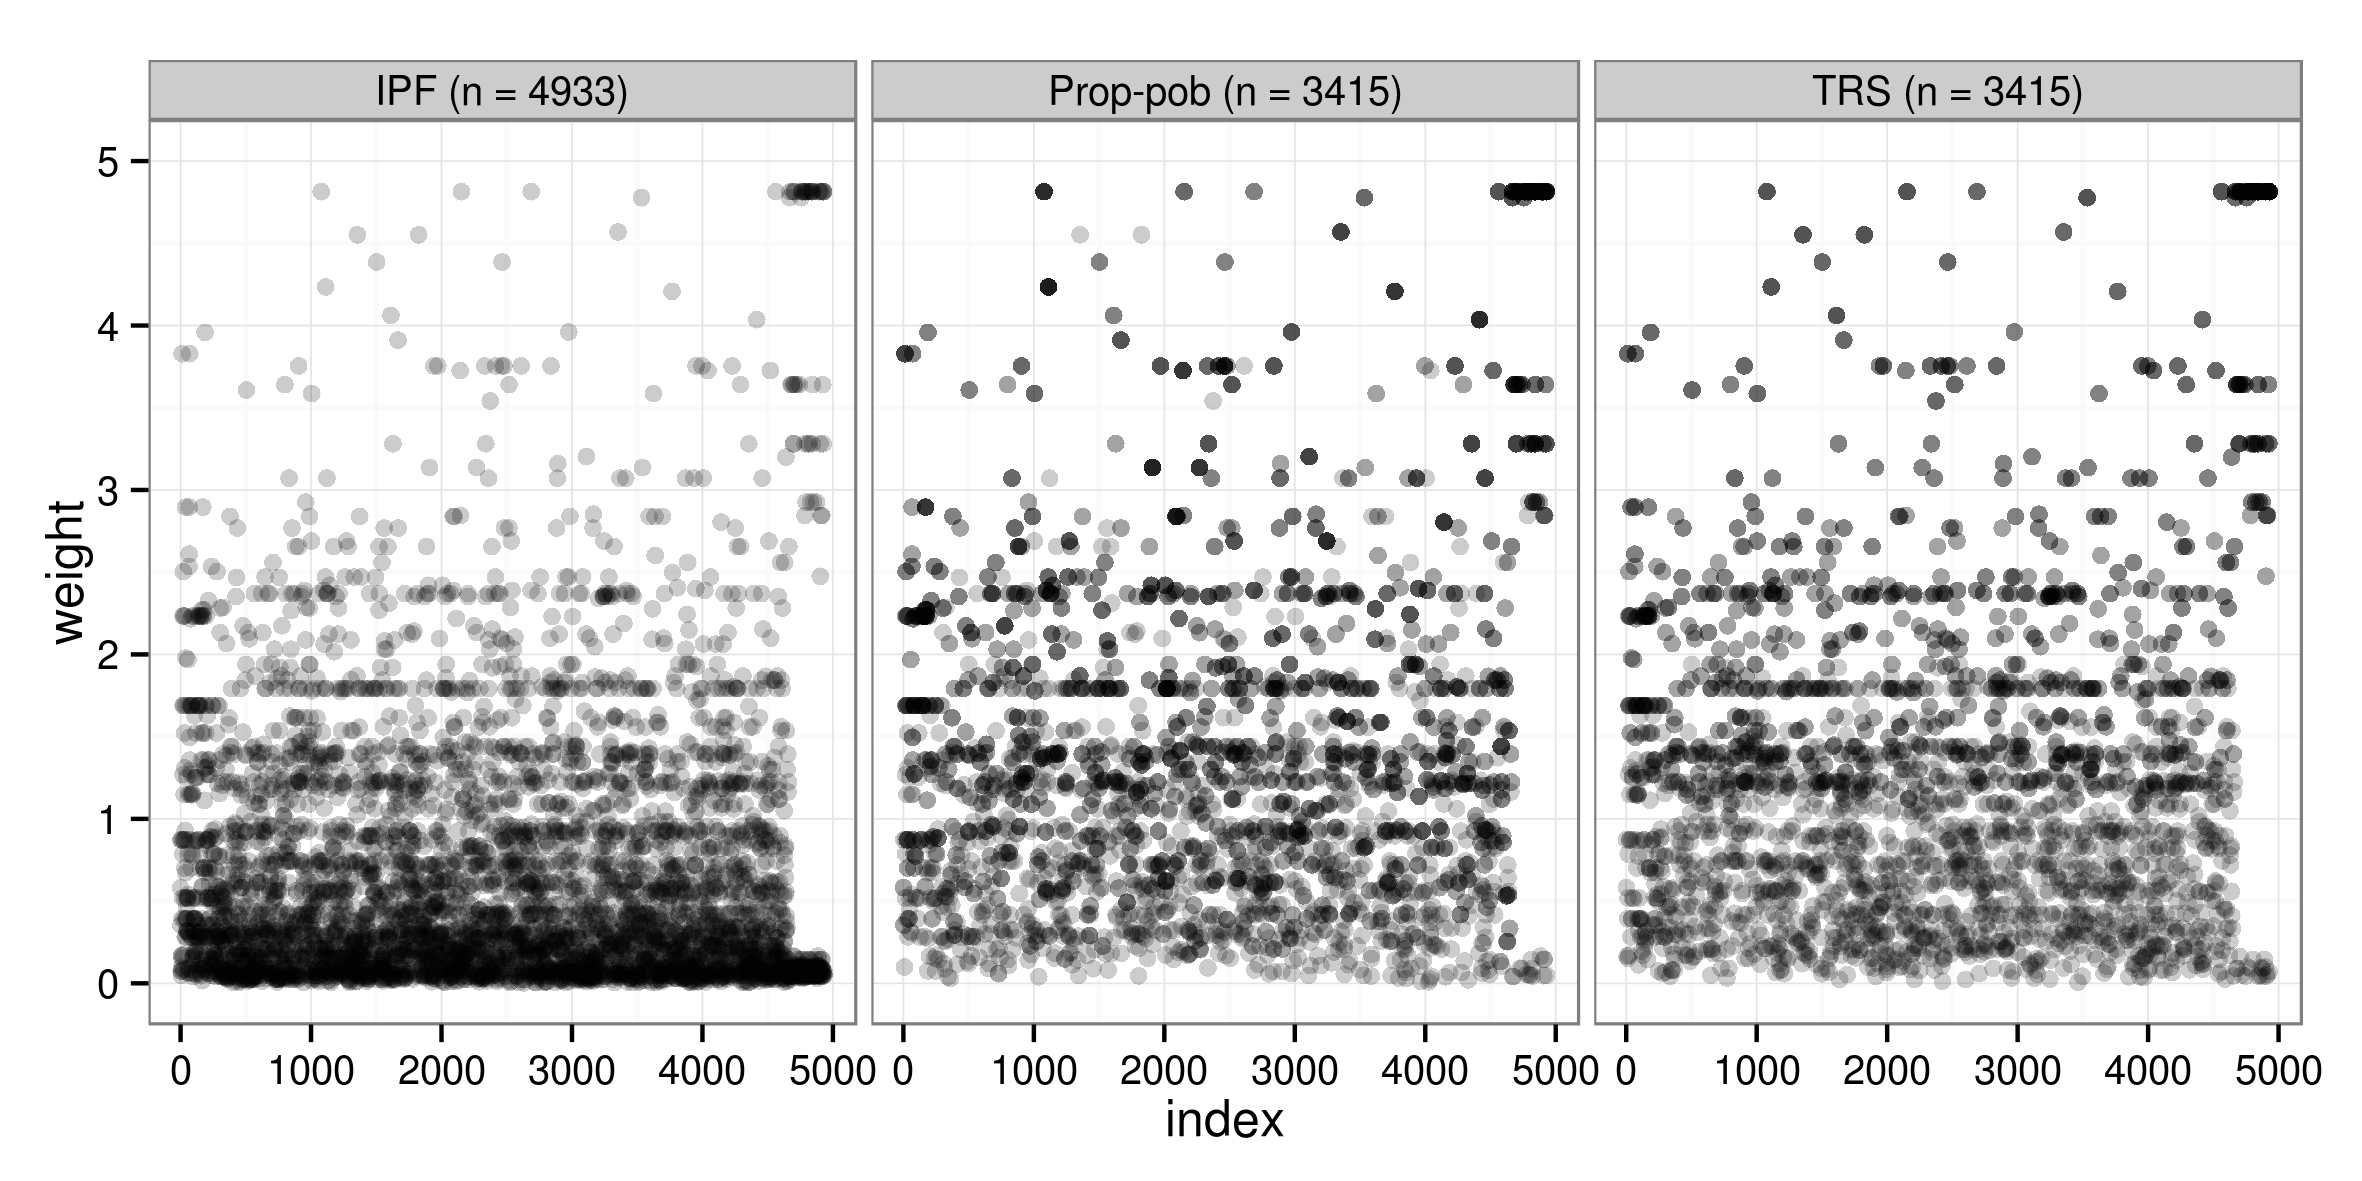
\includegraphics[width=12 cm]{IvW2}}
 % hist-weights.pdf: 792x612 pixel, 72dpi, 27.94x21.59 cm, bb=0 0 792 612
 \caption[Overplotted scatter graphs of index against weight]{Overplotted
scatter graphs of index against weight  for the original IPF weights (left) and
after proportional  probabilities (middle) and TRS (right) integerisation for
zone 71. Compare with Fig.~\ref{fig:threshweights}.}
 \label{fig:index-weight-TRS}
\end{figure}

Fig.~\ref{fig:index-TRS} illustrates the mechanism by which the TRS sampling
strategy works to select individuals. In the first stage (up to x = 1,717,
in this case) there is a linear
relationship between the indices of survey and sampled individuals, as the
model iteratively moves through the individuals, replicating those with
truncated weights greater than 0. This
(deterministic) replication stage selects roughly half of the required
population
in our example dataset (this proportion varies from zone to zone).
The next stage is probabilistic sampling
(x = 1,718 onwards in Fig.~\ref{fig:index-TRS}): individuals are selected from
the entire microdataset with selection probabilities equal to weight remainders.


\begin{figure}[h]
 \centerline{
 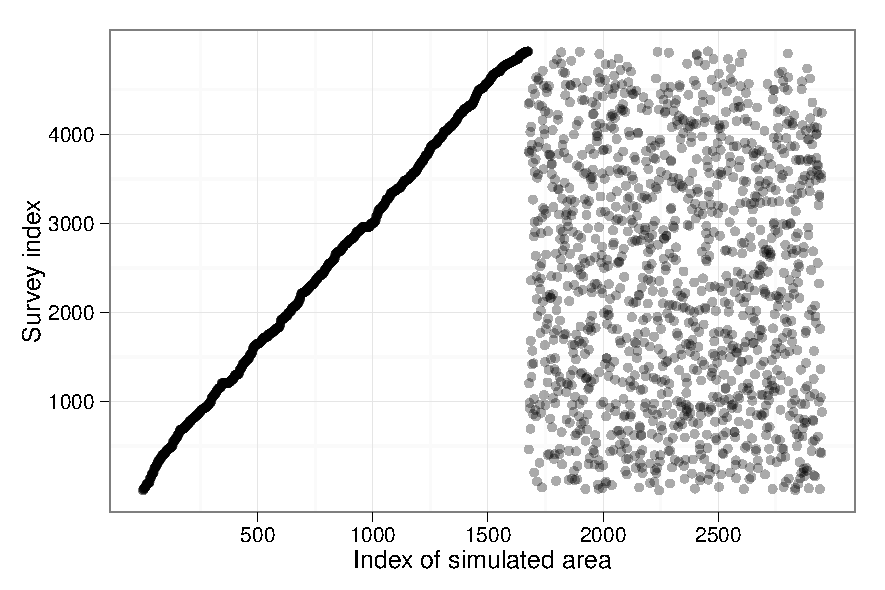
\includegraphics[width=12 cm]{indexes.pdf}}
 % hist-weights.pdf: 792x612 pixel, 72dpi, 27.94x21.59 cm, bb=0 0 792 612
 \caption[Scatter graph of the index values of individuals]{Scatter graph of the
index values of individuals in the original sample and their indices following
TRS Integerisation for a single area. }
 \label{fig:index-TRS}
\end{figure}

\subsubsection{The test scenario: input data and IPF}
\label{worked-eg}
% In order to test integerisation techniques, they were tested on a real world
% example. This section serves two functions: to illustrate the utility of
% integerisation techniques when modelling continuous variables using spatial
% microsimulation, and to describe how the integerisation
% techniques were tested.
The theory and methods presented above demonstrate how five integerisation
methods work in abstract terms. But to compare them quantitatively a test
scenario is needed. This example consists of a spatial microsimulation model
that uses IPF to model the commuting and socio-demographic characteristics
of economically active individuals in
Sheffield. According to the 2001 Census, Sheffield has a working
population of just over 230,000. The characteristics of these
individuals were simulated by reweighting a synthetic microdataset based on
aggregate constraint variables provided at the medium super output area (MSOA)
level. The synthetic microdataset was created by `scrambling' a subset of the
Understanding Society dataset (USd).\footnote{See
http://www.understandingsociety.org.uk/. To scramble this data, the continuous
variables (see Table \ref{t:data}) had an integer random number (between 10 and
-10) added to them; categorical variables were mixed up, and all other
information was removed.} MSOAs
contain on average
just over 7,000 people each, of whom 44\% are economically active
in the study area; for the less sensitive aggregate constraints, real data were
used. These variables are summarised in Table \ref{t:data}.

\begin{table}[htbp]
\caption{Summary data for the spatial microsimulation model}
\begin{center}
\begin{tabular}{lrlll}
\toprule
 & \multicolumn{ 2}{c}{\textbf{Aggregate data}} & \multicolumn{
2}{c}{\textbf{Survey data}} \\
 & \multicolumn{ 2}{c}{71 zones, average pop.: 3077.5} & \multicolumn{
2}{c}{4933 observations} \\ \midrule
Variable & \multicolumn{1}{l}{N. categories} & Most populous  & Mean  &
Most populous \\ \hline
Age / sex  & 12 & Male, 35 to 54 yrs & \multicolumn{1}{r}{40.1} & - \\
Mode  & 11 & Car driver & - & Car driver \\
Distance  & 8 & 2 to 5 km & \multicolumn{1}{r}{11.6} & - \\
NS-SEC  & 9 & Lower managerial & - & Lower managerial \\ \bottomrule
\end{tabular}\end{center}
\label{t:data}
\end{table}

The data contains both continuous (age, distance) and categorical (mode,
NS-SEC) variables. In practice, all variables are converted into categorical
variables for the purposes of IPF, however. To do this statistical
bins are used.
Table \ref{t:data} illustrates similarities between aggregate
and survey data overall (car drivers being the most popular mode of travel to
work in both categories, for example). Large differences exist between
individual zones and survey data, however: it is the role of iterative
proportional fitting to apply weights to minimize these differences.

IPF was used to assign 71 weights to
each of the 4,933 individuals, one weight for each zone. The fit
between census and weighted microdata can be seen
improving after constraining by each of the 40 variables
(Fig.~\ref{fig:IPF-4c}).
The process is repeated until an adequate level
of convergence is attained (see Fig.~\ref{fig:ipf-scat}).\footnote{What
constitutes an `adequate' level of fit has not been well defined in the
literature, as mentioned in the next section. In this example, 20
iterations were used.}
\begin{figure}[h]
 \centerline{
 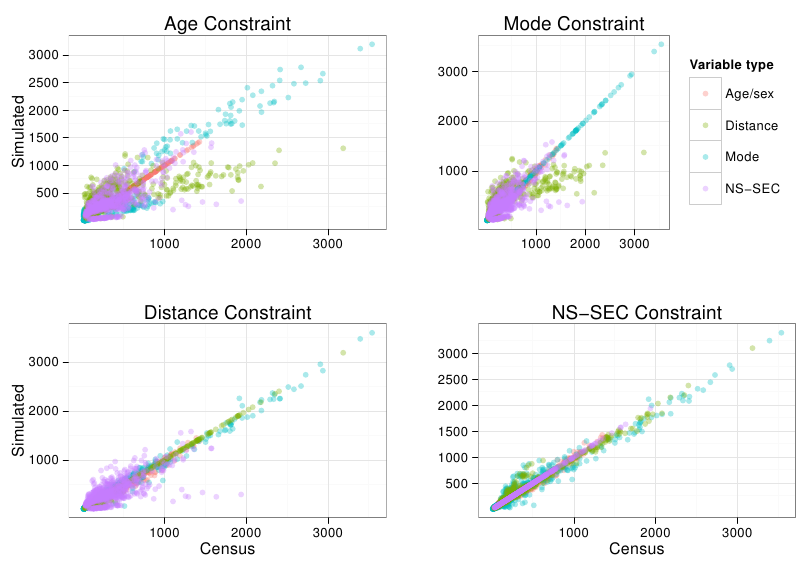
\includegraphics[width=14 cm]{IPF-4c2}}
 % hist-weights.pdf: 792x612 pixel, 72dpi, 27.94x21.59 cm, bb=0 0 792 612
 \caption[Visualisation of IPF method]{Visualisation of IPF method. The graphs
show the iterative
improvements in fit after age, mode, distance and finally NS-SEC constraints
were applied (see Table \ref{t:data}). See footnote 4 for resources on how IPF
works.}
 \label{fig:IPF-4c}
\end{figure}
The weights were set to an initial value of
one.\footnote{An initial value must be selected for IPF to create new weights
which better match the small area constraints.
It was set to one as this tends to be the average weight value in social surveys
(the mean Understanding Society dataset interview plus proxy individual
cross-sectional weight is 0.986).}
The weights were then iteratively
altered to match the aggregate (MSOA) level statistics.

\begin{figure}[h]
 \centerline{
 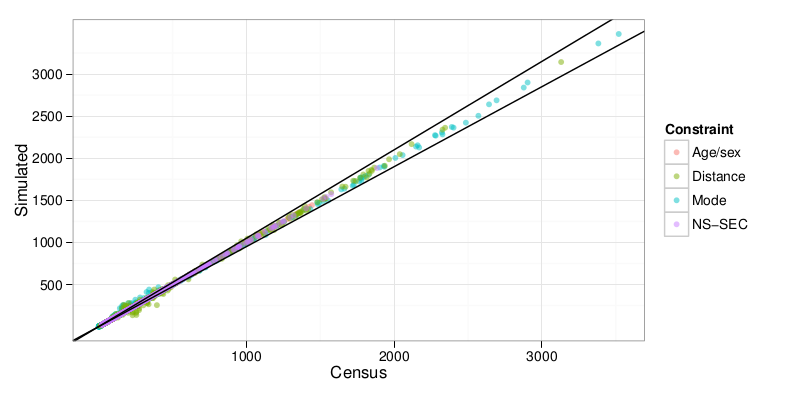
\includegraphics[width=13 cm]{ipf-scat2}}
 % hist-weights.pdf: 792x612 pixel, 72dpi, 27.94x21.59 cm, bb=0 0 792 612
 \caption[Scatter graph illustrating the fit between census and simulated
aggregates]{Scatter graph illustrating the fit between census and simulated
aggregates after 20 IPF iterations (compare with Fig.~\ref{fig:IPF-4c}).}
 \label{fig:ipf-scat}
\end{figure}

Four constraint variables link the aggregated census data to the survey,
containing a total of 40 categories. To illustrate how IPF works, it is useful
to inspect the fit between simulated and census aggregates before and after
performing IPF for each constraint variable. Fig.~\ref{fig:IPF-4c}
illustrates this process for each constraint. By contrast to existing
approaches to visualising IPF (see \citealp{Ballas2005b}), Fig.
\ref{fig:IPF-4c} plots the results for all variables, one
constraint at a time. This approach can highlight which constraint variables
are particularly problematic. After 20
iterations (Fig.~\ref{fig:ipf-scat}), one can see that distance and mode
constraints are most problematic. This may be because both variables depend
largely on geographical location, so are not captured well by UK-wide
aggregates.

Fig.~\ref{fig:IPF-4c} also illustrates how IPF works: after reweighting for
a particular constraint, the weights are forced to take values such that the
aggregate statistics of the simulated microdataset match perfectly with the
census aggregates, for all variables within the constraint in question.
Aggregate values for the mode variables, for example, fit the census results
perfectly after constraining by mode (top right panel in Fig.
\ref{fig:IPF-4c}). Reweighting by the next constraint disrupts the fit
imposed by the previous constraint --- note the increase scatter of the (blue)
mode variables after weights are constrained by distance (bottom left).

However, the disrupted fit is better than the original. This leads to
a convergence of the weights such that the fit between simulated and known
variables is optimised:
% The fit after each complete iteration can be formally measured in
% absolute and relative terms. The latter case is illustrated in Fig.~\ref{}
Fig.~\ref{fig:IPF-4c} shows that accuracy increases after weights are
constrained by each successive linking variable.
% % %\ref{fig:ints-errors},
% % %which shows how accuracy (measured as the proportion of simulated results
% % %falling beyond 5\% above or below the census value, as illustrated in
% % \ref{fig:4hists}, which shows continual improvement in model fit: the
% % distribution of residuals tend to 0 with each successive iteration.
% %
% % The results also show, however, that
% % some variables create more error than other --- the results of reweighting
% % the constraint ``mode'' are always worse than obtained by reweighting by the
% % other variables. This is significant because it means that the final results
% of
% % IPF models may depend more on the order of the constraint variables than on
% the
% % number of iterations.
%
% %  \begin{figure}[t]
% %  \centerline{
% %  \includegraphics[width=14 cm]{its-errors.pdf}}
% %  % hist-weights.pdf: 792x612 pixel, 72dpi, 27.94x21.59 cm, bb=0 0 792 612
% %  \caption{Proportion of results that fall beyond 5\% of the census values
% after
% % reweighting by each constraint variable over 10 complete iterations.}
% %  \label{fig:ints-errors}
% % \end{figure}

\subsection{Results}
\label{results}
This section compares the five previously describe approaches to
integerisation --- rounding, inclusion threshold, counter-weight, proportional
probabilities  and TRS methods. The results are based on the 20$^{th}$
iteration of the IPF model described above. The following metrics of
performance were assessed:
\begin{itemize}
 \item speed of calculation
\item accuracy of results
\begin{itemize}
 \item sample size
%: does the integer microsimulation sample size match the actual population?
\item Total Absolute Error (TAE) of simulated areas
\item anomalies (aggregate cell values out by more than 5\%)
\item correlation between constraint variables in the census and
microsimulated data.
\end{itemize}
\end{itemize}

Of these performance indicators accuracy is the most problematic.
Options for measuring goodness-of-fit have proliferated in the last two decades,
yet there is no consensus about which is most appropriate \citep{Voas2001}.
The approach taken here, therefore, is to use a range of measures, the most
important of which are summarised in Table \ref{acc-results} and Fig.
\ref{fig:3scat}.

\begin{figure}[h*]
 \centerline{
 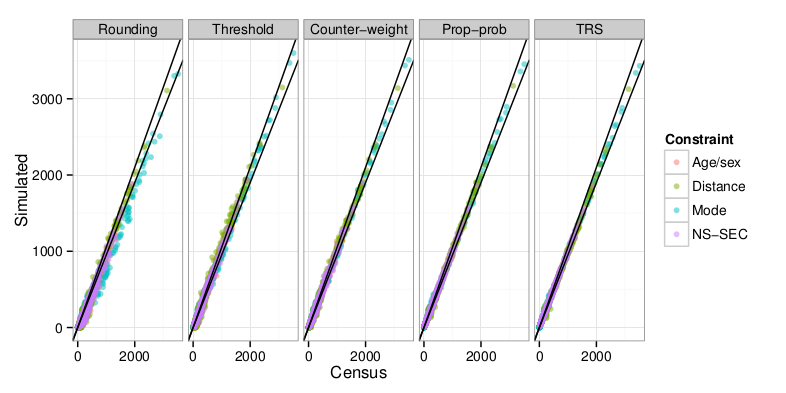
\includegraphics[width=13.5 cm]{ints-5scat-ab}}
 % hist-weights.pdf: 792x612 pixel, 72dpi, 27.94x21.59 cm, bb=0 0 792 612
 \caption[Scatterplots of actual (census) and simulated population
totals]{Scatterplots of actual (census) and simulated population totals for four
integerisation techniques. The black lines represent 5\% error in either
direction. }
 \label{fig:3scat}
\end{figure}

\subsubsection{Speed of calculation}
%With modern desktop computers, computational requirements is less frequently
The time taken for the integerisation of IPF weights was measured on an Intel
Core i5 660 (3.33 GHz) machine with 4 Gb of RAM running Linux 3.0.
The simple rounding method of integerisation was unsurprisingly the fastest, at
4 seconds. % Add c-w time
In second and third place respectively were the proportional probabilities
and TRS approaches, which took a couple of seconds longer for a single
integerisation run for all areas.
Slowest were the inclusion threshold and counter-weight techniques, which took
three times longer than simple rounding. To ensure representative results for
the probabilistic approaches, both were run 20 times and the result with the
best fit was selected. These imputation loops took just under a minute.

The computational intensity of integerisation may
be problematic when processing weights for very large
datasets, or using older computers. However, the results must be placed in
the context of the computational requirements of the IPF process itself. For the
example described in Section \ref{worked-eg}, IPF took approximately
30 seconds per iteration and 5 minutes for the full 20 iterations.

\subsubsection{Accuracy}
In order to compare the fit between simulated microdata and the zonally
aggregated linking variables that constrain them, the former must first be
aggregated by zone. This aggregation stage allows the fit between linking
variables to be compared directly (see Fig.~\ref{fig:3scat}). More
formally, this aggregation allows goodness of fit to be calculated using a range
of metrics \citep{Williamson1998}. We compared the accuracy of integerisation
techniques using 5 metrics:
\begin{itemize}
\item Pearson's product-moment correlation coefficient ($r$)
\item total and standardised absolute error (TAE and SAE),
\item proportion of simulated values falling beyond 5\% of the actual values,
% This is the standard measure
% of correlation and requires no further explanation here \citep{Rodgers1988}.
\item the proportion of Z-scores significant at the 5\% level
\item size of the sampled populations
\end{itemize}

The simplest way to evaluate the fit between simulated and census results
was to use Pearson's $r$, an established measure of association
\citep{Rodgers1988}.
The $r$ values for all constraints were 0.9911, 0.9960, 0.9978,
0.9989 and 0.9992 for rounding, threshold, counter-weight, proportional
probabilities and TRS
methods respectively. IPF alone had an $r$ value of 0.9996. These correlations
establish an order of fit that can be compared to other metrics.

TAE and SAE are crude yet effective measures of overall
model fit \citep{Voas2001}. TAE has the additional advantage of
being easily understood:
\begin{equation}
 TAE = \sum\limits_{ij}|U_{ij} - T_{ij}|
 \label{etae}
\end{equation}
where U and T are the observed and simulated values for each linking variable
($j$) and each area ($i$).
% Change 34 (symbol: % Change): converted TEA to TAE
SAE is the TAE divided by the total
population of the study area. TAE is sensitive to the number of people
within the model, while SAE is not. The latter is seen by \citet{Voas2001} as
``marginally preferable'' to the former: it allows cross-comparisons between
models of different total populations \citep{Kongmuang2006-thesis}.

\begin{table}[]
\caption{Accuracy results for integerisation techniques.*}
\small{
\begin{center}
\begin{tabular}{llrrrr}
\toprule
Method & Variables & \multicolumn{1}{l}{TAE} & \multicolumn{1}{l}{SAE (\%)} &
\multicolumn{1}{l}{E $>$ 5\% (\%)} & \multicolumn{1}{l}{$Z{m}^{2}$ (\%)} \\
\midrule
IPF & Age/sex & 9 & 0.0 & 0.0 & 0.0 \\
 & Distance & 4874 & 2.3 & 13.7 & 4.9 \\
 & Mode & 4201 & 2.0 & 6.4 & 4.2 \\
 & NS-SEC & 0 & 0.0 & 0.0 & 0.0 \\
\textbf{} & \textbf{All} & \textbf{9084} & \textbf{3.1} & \textbf{4.5} &
\textbf{2.1} \\
\midrule
Round- & Age/sex & 26812 & 12.5 & 81.5 & 39.8 \\
 ing& Distance & 31981 & 14.9 & 80.1 & 65.1 \\
 & Mode & 30558 & 14.2 & 81.4 & 48.9 \\
 & NS-SEC & 27493 & 12.8 & 76.5 & 57.1 \\
 & \textbf{All} & \textbf{116844} & \textbf{13.6} & \textbf{80.1} &
\textbf{51.3} \\
\midrule
Thresh- & Age/sex &  11076 & 5.1 & 49.2 & 8.1 \\
 old& Distance & 27146 & 12.6 & 82.4 & 57.7 \\
 & Mode & 14770 & 6.9 & 68.6 & 33.9 \\
 & NS-SEC & 13770 & 6.4 & 55.2 & 24.1 \\
 & \textbf{All} &  \textbf{66762} & \textbf{7.8} & \textbf{62.5} & \textbf{28.7}
\\
\midrule
Counter- & Age/sex & 10242 & 4.8 & 47.7 & 6.6 \\
weight& Distance &  17103 & 8.0 & 70.2 & 39.3 \\
 & Mode &  10072 & 4.7 & 60.4 & 21.6 \\
 & NS-SEC & 11798 & 5.5 & 49.6 & 17.1 \\
 & \textbf{All} & \textbf{49215} & \textbf{5.7} & \textbf{56.1} & \textbf{19.6}
\\
\midrule

Propor- & Age/sex & 9112 & 4.2 & 48.0 & 3.1 \\
tional & Distance & 8740 & 4.1 & 47.4 & 10.4 \\
proba- & Mode & 8664 & 4.0 & 60.8 & 9.0 \\
bilities & NS-SEC & 7778 & 3.6 & 37.6 & 3.3 \\
 & \textbf{All} & \textbf{34294} & \textbf{4.0} & \textbf{49.0} & \textbf{6.2}
\\
\midrule
TRS &Age/sex & 5424 & 2.5 & 27.9 & 0.4 \\
 & Distance & 10167 & 4.7 & 48.8 & 16.4 \\
 & Mode & 7584 & 3.5 & 56.1 & 6.7 \\
 & NS-SEC & 5687 & 2.6 & 24.9 & 1.1 \\
 & \textbf{Total} & \textbf{28862} & \textbf{3.4} & \textbf{39.2} & \textbf{5.5}
\\
\bottomrule
\end{tabular}
\end{center}
}
\label{acc-results}
\begin{tablenotes}
      \footnotesize
      \item * The probabilistic
results represent the best fit (in terms of TAE) of 20 integerisation runs
with the pseudo-random number seed set to 1000 for replicability --- see
Supplementary Information.
    \end{tablenotes}
\end{table}

The proportion of values which fall beyond 5\% of the actual values is a simple
metric of the quality of the fit. It implies that getting a perfect fit is not
the aim, and penalises fits that have a large number of outliers. The precise
definition of 'outlier' is somewhat arbitrary (one could just as well use 1\%).

The final metric presented in Table \ref{acc-results}
is based on the Z-statistic, a standardised measure of
deviance from expected values, calculated for each cell of data. We use $Zm$, a
modified version of the Z-statistic which is a robust measure of fit for each
cell value \citet{Williamson1998}. The measure of
fit is appropriate here as it takes into account absolute, rather than just
relative, differences between simulated and observed cell count:
\begin{equation}
 Zm_{ij} = (r_{ij} - p_{ij}) \Bigg/ \left(\frac{p_{ij}(1 -
p_{ij}))}{\sum\limits_{ij}U_{ij}}\right)^{1/2}
\end{equation}

where

\begin{center}
\begin{math}
  p_{ij} = \frac{U_{ij}}{\sum\limits_{ij}U_{ij}} \qquad and \qquad r_{ij} =
\frac{T_{ij}}{\sum\limits_{ij}U_{ij}}
\end{math}
\end{center}

To use the modified Z-statistic as a measure of overall model fit, one simply
sums the squares of $zm$ to calculate $Z{m}^{2}$. This measure can handle
observed cell counts below 5, which chi-squared tests cannot \citep{Voas2001}.

The results presented in Table \ref{acc-results} confirm that \emph{all}
integerisation methods introduce
some error. It is reassuring that the comparative accuracy is the same across
all metrics. Total absolute error (TAE), the simplest goodness-of-fit
metric, indicates that discrepancies between simulated and census data increase
by a factor of 3.2 after TRS integerisation, compared with raw
(fractional) IPF weights.\footnote{In the case of a sufficiently diverse input
survey dataset, IPF would be able to find the perfect solution: TAE would be 0
and the ratio of error would not be
applicable.}
Still, this is a
major improvement on the simple rounding, threshold and counter-weight
approaches to integerisation presented by \citet{Ballas2005c}: these increased
TAE by a factor of 13, 7 and 5 respectively.
The improvement in fit relative to the proportional probabilities method
is more modest. The proportional probabilities method increased TAE by a factor
of 3.8, 23\% more absolute error than TRS.

The differences between the simulated and actual populations ($Pop_{sim} -
Pop_{cens}$) were also calculated for
each area. The resulting differences are summarised in Table 5, which
illustrates that the counter-weight and two probabilistic methods resulted
in the correct population totals for every area. Simple rounding and threshold
integerisation methods greatly underestimate and slightly overestimate the
actual populations, respectively.

\begin{table}[h*]
\begin{center}
\caption{Differences between census and simulated populations.}
\vspace{0.25 cm}
\begin{tabular}{lrrr}
\toprule
Metric & \multicolumn{1}{l}{Rounding} & \multicolumn{1}{l}{Threshold} &
\multicolumn{1}{l}{Others (CW, PP, TRS)} \\ \midrule
Mean & -372 & 8 & 0  \\
Standard deviation & 88 & 11 & 0 \\
Max & -133 & 54 & 0 \\
Min & -536 & 0 & 0 \\
Oversample (\%) & -13 & 0.3 & 0 \\
\bottomrule
\end{tabular}
\end{center}
\label{t:pops}
\end{table}




\subsection{Discussion and conclusions}
\label{discuss}
The results show that TRS integerisation outperforms the other methods of
integerisation tested in this section.
At the aggregate level, accuracy
improves in the following order: simple rounding,
inclusion threshold, counter-weight, proportional probabilities and, most
accurately, TRS. This order of preference remains unchanged, regardless of which
(from a selection of 5) measure of goodness-of-fit is used. These results
concur with a finding derived from theory --- that ``deterministic rounding of
the counts is not a satisfactory integerization''
\citep[p.~689]{Pritchard2012}.
Proportional probability and TRS methods clearly provide more accurate
alternatives.

An additional advantage of the probabilistic TRS and proportional probability
methods is that correct population sizes are guaranteed.\footnote{Although
the counter-weight method produced the correct population sizes in our tests, it
cannot be guaranteed to do so in all cases, because of its reliance on simple
rounding: if more weights are rounded up than down, the population will be too
high. However, it can be expected to yield the correct population in cases
where the populations of the areas under investigation are substantially
larger than the number of individuals in the survey dataset.}
In terms of speed of calculation, TRS also performs well. TRS takes marginally
more time than simple rounding and proportional probability methods,
but is three times quicker than the threshold and counter-weight
approaches. In practice, it seems that integerisation processing time is
small relative to running IPF over several iterations. Another
major benefit of these non-deterministic methods is that probability
distributions of results can be generated, if the algorithms are run multiple
times using unrelated pseudo-random numbers. Probabilistic methods could
therefore enable the uncertainty introduced through integerisation to be
investigated quantitatively
\citep{Beckman1996, Rubin1987} and subsequently illustrated using error bars.

Overall the results indicate that TRS is superior to the
deterministic methods on many levels and introduces less error than the
proportional probabilities approach.
We cannot claim that TRS is `the best' integerisation strategy available though:
there may be other solutions to the problem and different sets of test weights
may generate different
results.\footnote{Despite these caveats, the order of accuracy
identified in this section is expected to hold in most cases.
Supplementary Information (Section 4.4), shows the same order of
accuracy (except the threshold method and counter-weight
methods, which swap places) resulting from the integerisation of a
different weight matrix.
}
The issue will still present a
challenge for future researchers considering the use of IPF to generate sample
populations composed of whole individuals: whether to use deterministic or
probabilistic methods is still an open question (some may favour
deterministic methods that avoid psuedo-random numbers, to ensure
reproducibility regardless of the software used), and the question of whether
combinatorial optimisation algorithms perform better has not been addressed.

Our results provide insight into the advantages and disadvantages of
five integerisation methods and guidance to researchers wishing to
use IPF to generate integer weights: use
TRS unless determinism is needed or until superior alternatives (e.g.~real small
area microdata) become available. Based on the code and example datasets
provided in the Supplementary Information, other are encouraged to use, build on
and improve TRS integerisation.

A broader issue raised by this research, that requires further
investigation before answers emerge, is `how do the integerised results of IPF
compare with combinatorial optimisation approaches to spatial microsimulation?'
Studies have compared non-integer results of IPF with
alternative approaches \citep{Smith2009, Ryan2009, Rahman2010, harland2012}.
However, these have so far failed to compare like with like: the integer results
of combinatorial approaches are more useful (applicable to more types of
analysis) than the non-integer results of IPF. TRS thus offers a
way of `levelling the playing field' whilst minimising the error introduced to
the results of deterministic reweighting through integerisation.

In conclusion, the integerisation methods presented in this section make
integer results accessible to those with a working knowledge of IPF. TRS
outperforms previously published methods of integerisation. As such, the
technique offers an attractive alternative to combinatorial
optimisation approaches for applications that
require whole individuals to be simulated based on aggregate data.

% \section{Visualisation techniques} \label{svis}
% Dump a load of R code and unused figures in here

% \section{Methods of including geography} %!!! include later!!!???
% 
% \section{Assigning work location} %Taken from vul-meth
% \label{s:workdes}
% \label{sflow} \index{flow data}
% So far the methods presented have been concerned primarily with
% individual level attributes such as mode (including type of car ownership),
% distance and class, despite the availability of additional geographical data
% (\cref{sadditional}). Other than chloropleth maps based on zonally aggregated
% data, the work has been largely
% non-geographical, as the spatial microdata
% %%% add a cross-ref to a table describing the data?
% are simply allocated to
% zones via an individual level `zone' variable, rather than being placed
% specifically on the map. Worse, the location of commuters' place of work is not
% considered at all in the preceding discussion.
% % Yet it is clear that % Include other geographic factors later
% % topography, congestion, driving habits and local employment
% % markets all affect the energy costs of commuting, and the impacts of its
% % variability.
% This section describes methods of incorporating this geographical
% knowledge into our models.
% % This will help enhance understanding of geographical
% % variation in the energy impacts.
% 
% % \subsection{Assigning work location} %Taken from vul-meth
% % \label{s:workdes}
% %  Original intro: weak
% % What is the spatial distribution of energy intensive commuter patterns? What
% % types of places are conducive to low-energy modes such as walking and cycling?
% % Intuition would suggest an urban-rural divide, and that transport
% % infrastructure would influence commuter patterns over space.
% % This subsection provides more rigorous methods to investigate the spatial
% % correlates of energy intensive commuter patterns.
% The spatial microsimulation model results in a large dataset containing
% hundreds of individuals for each zone under investigation. For micro level
% spatial analysis, origin-destination pairs are needed: simulated
% places of home and work need to be geotagged. The simplest solution
% to this problem is to allocate all individuals in each zone home coordinates
% corresponding to the zone's population-weighted centroid. Likewise, work
% coordinates can be assumed to be the nearest employment centre, as described in
% \cref{sremotness}. This method allows for simple analyses such as the proxy for
% geographic isolation presented in Fig.~\ref{fig:dis-msoa}.
% 
% \begin{figure}
% \begin{center}
%   \includegraphics[width = 13 cm]{distances-msoa2}
% \end{center}
% \caption[Average distance to employment centre in South Yorkshire]{Average
% distance to employment centre in South Yorkshire. The
% left-hand map illustrates how distance was calculated (using the command
%  nncross() in the R package `spatstat'). The right-hand map illustrates
% the results --- Sheffield and Rotherham are grouped together in the same
% travel to work zone.}
% \label{fig:dis-msoa}
% \end{figure}
% 
% Rather than assuming that work centres are always located in the city
% centre, a more realistic approach is to acknowledge that a variety of
% employment centres exist, and that the relative importance of each varies from
% place to place. This is illustrated in Fig.~\ref{fig:sflow}, a flow diagram of
% the work locations of commuters based on the outskirts of Sheffield. Although
% Barnsley is the closest city centre to Stocksbridge (see
% Fig.~\ref{fig:dis-msoa}), this analysis makes it clear that Sheffield is the
% primary non-home workplace.
% 
% \begin{figure}
% \centering{
%  \includegraphics[width = 10 cm]{sflows}}
% \caption[Flow diagram illustrating popular commuter destinations for citizens
% of Stocksbridge]{Flow diagram illustrating popular commuter destinations for
% citizens
% of Stocksbridge. The thickness of the lines is proportional to the number of
% people who travel there (for reference, 661 people travel to
% the centre of Sheffield --- illustrated by the thickest line ---
% and 2036 people work in Stocksbridge --- illustrated by the dot
% from which all lines radiate. n = 6,338).}
% \label{fig:sflow}
% \end{figure}
% 
% The analyses presented in both Fig.~\ref{fig:dis-msoa} and Fig.~\ref{fig:sflow}
% both greatly oversimplify trip routes. The straight lines underestimate travel
% distance, completely ignoring the transport network. A more
% realistic method is to randomly allocate each individual to a unique home
% location based on
% % data on houses, and work
% % locations based on commuter flow data and the distance they travel to work
% population density (or, potentially, local area classification) and estimate
% the route taken using shortest trip algorithms dependent on the mode of
% transport used (\cref{fig:agent}). This latter method allows for the
% calculation of route distances by mode, but is more complex and difficult to
% implement over large areas.
% %\footnote{?}
% The method used to model the home-work flows presented in \cref{fig:agent},
% following the transport network, was as follows:
% \begin{itemize}
%  \item Allocate home locations to individuals in each ward. This was done
% by a stratified sample allocating individuals to smaller OA zones. Simple
% random sampling, using QGIS, created points within each zone.\footnote{This
% technique is not ideal for a couple of reasons. First, output areas do not all
% have the same working population, so it is not strictly true to say that the
% probabilities of inhabiting any of them is the same. (The mean and standard
% deviation of the working population of all 165,665 OAs in England in the 2001
% Census is 136 and 43, respectively and ranges from 0 for an area in East Dorset
% to 2121 in an area in Telford.) This problem could be easily be overcome by
% setting the number of points sampled for each OA proportional to their commuting
% population. A more severe problem for extensive OAs is that the selected points
% are unlikely to be actual houses; people could be allocated home coordinates in
% forests, mountains or even rivers as OAs provide contiguous geographical
% coverage. Methods for allocating individuals to residential building layers,
% instead of anyway, are being developed (as of December 2013) at the University
% of Southamption (Alan Smith, 2013, personal communication.)
% }
% \item Allocate a work destination for each individual. This was done by: 1)
% allocating the destination work location to concentric rings surrounding the
% ward centroid (\cref{fig:agent}); 2) randomly allocating the
% destination to a destination whose centroid lies within the allocated distance
% band, with the probability set proportional to the flow to that destination
% (from Nomis flow data); and 3) randomly selecting a point from the destination
% ward.\footnote{Work location could be allocated more precisely using the same
% technique, but harnessing the OA flow data illustrate in \cref{flows2bigemps}.}
% \item Calculating the route distance using the QGIS ``Road graph'' plugin. The
% network data for pedestrians and cars was loaded from a PostGIS database of OSM
% data; pedestrians and cyclists used the pedestrian part of the network; all
% other users used the road network.\footnote{Ideally, an automated
% batch-processing of shortest route would be used instead of the GUI of Road
% graph. This would allow more than 20 routes to be calculated. The route-planning
% Routino software was designed for use on the OSM network, so would be ideal for
% this purpose.}
% \item Save the results in an individual level variable.
% \end{itemize}
% The penultimate step in this process was the most problematic. It took a long
% time to import the OSM route network into a format that Road graph could
% understand, and each shortest route calculation took around 10 seconds (far
% longer than Google's routing service). Also, the two-way division of the
% transport network is not realistic: bicycles cannot follow all pedestrian paths
% and trains can clearly not follow roads. In addition, evidence from GPS traces
% suggests that in many cases the shortest route is not in fact the one taken
% (e.g.~\citealp{Ehrgott2012}). None of these difficulties are intractable,
% especially as the OSM transport network and software to handle it continue to
% improve.\footnote{The trip planning platform
% \href{http://opentripplanner.com/}{OpenTripPlanner} is a good example of this
% as it is rapidly developing multi-mode trip planning capabilities worldwide,
% base on the OSM and local authority data. The capability of this software can
% be tested on the \href{http://london.optitrans.net/}{Optitrans} website, a
% London-based multi-mode routing service.}
% Due to time constraints and the immaturity of some of the software used to
% batch process optimal routes, however, routing was omitted from the central
% calculation of energy costs. The impact of route choice on energy costs are
% further discussed in \cref{Chapter6}.
% 
% % \footnote{This analysis results from 20 randomly selected
% % individuals (2 of
% % whom worked at home) from the spatial microsimulation model output for
% % Stocksbridge and allocated origin-destination points based on known distance
% % bands, ward-ward commuter flows, and the population density distribution of
% % Stocksbridge.
% % }
% 
% \begin{figure}
%  \includegraphics[width = 13 cm]{agents4}
% \caption[Simulated route choice for 20 randomly selected individuals]{Simulated
% route choice for 20 randomly selected individuals
% from the spatial simulation model. Destinations were determined by 1) subsetting
% destination wards by distance from Stocksbridge centre, 2) assigning
% probabilities of working in each ward for each distance band (based on flow
% data presented in Fig.~\ref{fig:sflow}) and 3) randomly selecting points
% within the resulting destination wards. (Workplaces of 2 people who work from
% home are not mapped).}
% \label{fig:agent}
% \end{figure}
% 
% % \subsection{Visualising flow data} % Should be in visualisation section!!!
% 
% 
 % Data and methods

 \chapter{Energy use in personal travel systems} % Could it be a paper?
% Keep it short and clean, culminating in the numbers used next section
% Something about WTT, WTW and TTW terminology
\label{Chapter5}
% \lhead{Chapter 5. \emph{Energy use in personal travel systems}}
\fancyhead[RO,LE]{Chapter 5. Energy use in personal travel systems} %2side
\fancyhead[RE,LO]{\thepage}
% \begin{quote}
% In 1992, UK gross mass movement was equivalent to each woman, man and child
% driving a fully loaded 38-tonne goods vehicle 1.4 km each day. Only 22\% of
% this mass movement was the actual productive movement of people and goods, the
% remainder being the incidental mass movement of [the] transport carriers
% themselves.
% \flushright{\citep[p.~xi]{Peake1994}}
% \end{quote}
The previous chapter described the data and methods needed to model the
diversity of commuting behaviours at individual and geographical levels.
This chapter shows how the results of spatial microsimulation can be
translated into information about energy use. Before any numbers are
presented, however, this chapter takes a brief detour to consider what
energy actually is, and how it gets `used' in personal transport
(\cref{sfundamentals}). This will ensure that the energy use estimates
presented later on are
interpreted correctly (and not oversimplified). Physical considerations also
help understand the potential for and limitations of technological advance
to reduce energy use into the future\citep{MacKay2009}. Future
efficiency gains, important in what-if scenarios, are tackled in \cref{s:eff-imps}.

As stated in the previous chapter, good official estimates of the energy costs of personal
travel overall, let alone for travel to work exclusively, are in short supply:
they are limited in terms of the modes covered, geographical resolution and
temporal coverage.
The approach used here, therefore, is to infer
energy use based on
behaviour:\footnote{The
alternative is to use energy use statistics directly.
Official data is limited here and unofficial, privately owned
data on the subject is also limited. Petrol
station data, for example,
has the potential to inform us about overall energy use in
general areas, but is limited by the fact that consumers can many miles to
access the cheapest fuel, long-distance refuelling, the impossibility
of disaggregating by reason for trip and the public inaccessibility of petrol
station sales data. There is, however, much potential for using this data
source more, as no energy-transport studies could be found that do.
}
the mode, distance and frequency of
travel to work. Of course, this requires good estimates of vehicles' energy use
per unit distance to convert the distance travelled into energy use. The best
official data source for this task are the CO$_2$ `emission factors'
compiled by the government department Defra which (bizarrely) appear
to be outside the remit of
the Department for Energy and Climate Change (DECC).
These emission factors, and the calculations that convert them into
energy units, are described in \cref{sdirecte}. The subsequent section presents
data and equations for estimating energy use at the system level, to include
the additional energy costs of fuel, road and vehicle production
(\cref{ssystemlevel}). Deeper analysis reveals that the energy use per mode
estimates presented in the preceding two sections
(e.g.~that buses use 2.13 MJ/pkm on fuel) are rather gross oversimplifications
of reality: there is strong evidence of substantial variability in energy use
for different \emph{types} of vehicle, driver, trip and road/guideway
conditions. Assumptions about frequency of trips to work each year also
have a large impact on estimated annual energy use due to commuting.
Evidence on these issues is reported, and their inclusion in the models
of energy use discussed, in \cref{svariable}. Building on this evidence-base,
\cref{s:eff-imps} and \cref{seffspace} discuss and attempt to quantify
changing `fleet efficiencies' of cars over time and space. %!!! just cars right?

% % Removed reference to sreale as it's a disctraction from finishing the PhD.
% % Also, didn't I refer to best, worst middle ests?
% Of course, even once all these factors are taken into account, there
% is still an element of uncertainty, especially given the limited 
% evidence on which the assumptions are based.
% This is the topic of \cref{sreale}, which explains the differences
% between real and reported efficiencies and concludes that upper, lower and
% central estimates of each energy use component should be reported, rather than a
% single answer. (Some of the underlying reasons for the inherent uncertainty
% of our energy use estimations are reported in \cref{sfundamentals}.)
% Does it?!!!
Finally, \cref{sfinal} concludes the chapter by reporting our best
estimates of energy use by mode,
which result from factors considered in the preceding sections. These
values are provided a section of their own, as they are used in subsequent
sections and are critical to the results of the model. Before looking at these
issues in detail, a few comments on complexity and the dominance of the car are
in order.

An idea that any naive reader should dispel immediately is that energy use in
transport is simple. It is complex, more so than energy use in industrial and
domestic settings, so energy use values must be treated with care.
There is no single `right', global or final answer to questions such as
``how much energy does a
person use per unit distance travelled?'' As with many such simplistic questions
asked of complex systems, the answer is `it depends', on how the question
is defined and a number of other factors, even before
considering spatial and temporal variation
\citep{Agency2005, Fels1973, Lenzen1999}. In rough descending order of importance, these
include the following, each of which is considered below:
% maybe add sections!!!
\begin{itemize}
 \item the make, model, and condition of the vehicle in use
 \item behavioural factors such as propensity to accelerate (which are in
 turn influenced by legal, cultural and economic factors, as well as obstacles such as traffic lights)
 \item the nature of the physical and road environment such as road surface, topography and traffic
 \item ambient conditions including temperature and wind
 \item circuity and straightness of roads
\end{itemize}
Because of the complexity of these interacting factors,
effort has been made to make it simple to update existing estimates of energy
use (or refine them by adding geographical variability) if and when better
energy use estimates emerge. (It is hoped that the estimates presented in this
section could spur better energy-in-transport reporting by government agencies.)
Another factor, not included in the above bullet points, that cross-cuts all
of them, is the system boundaries of energy analysis: energy use will increase
(in some cases substantially) as the indirect costs of fuel,
vehicle, road/path construction and even unquantifiable knock-on impacts of
our transport systems are included. This becomes apparent when
the fundamentals of energy use in transport (\cref{sfundamentals}) are
considered. This is another reason for producing several estimates
% (which depend on where the
% system boundaries are drawn)
for each mode of transport when calculating energy
use in transport models, allowing sensitivity
analysis and scenarios of the future that incorporate the indirect energy costs
of transport.
% Footnote possible here on how this is recommended - up by 20% including
% consumption

The final introductory comment is that this chapter dedicates more attention to
cars than to other modes. This is a deliberate decision: cars totally dominate
the energy costs of commuting, using over 20 times more energy than all other modes
put together. \index{car}
% !!! cross-reference this

\section{Fundamentals of energy use in transport} \label{sfundamentals}
\index{energy}
Energy is an objective and quantifiable concept that spans the sciences.
Frequently the term is defined loosely as the `ability to do work', but this
raises the question: work on what? and fails to convey the importance of energy
for both the physical sciences and modern life \citep[p.~99]{Rouse1975}:
\begin{quotation}
 As we view the physical world, we find that energy is one of the most
fundamental and important concepts in science. Energy is essential to our
everyday experience. From the time we turn off the electric alarm clock to the
time we jump into our automobiles, ... until we sit down to the evening meal,
the use of energy in various forms is a central feature of our daily activity.
\end{quotation}
This quote reinforces the reasons set out for the energy focus laid-down in the
introduction, and adds a new one: we depend on energy. How different would
daily life be in the absence of continuous flows of concentrated energy?
The above quote illustrates how embedded external (and often invisible)
energy sources have become in our life. Later in the book, \citet{Rouse1975} urge
others to shed light on energy costs of different processes, in the context of
the 1970s oil crisis. In the context of 21$^{st}$ century environmental change
and fossil fuel depletion, this thesis --- by focussing the method on
energy use --- seeks to follow in the footsteps
of other researchers who sought to use energy as a yardstick against which to quantify
and evaluate complex processes.\footnote{Other pioneers of energy-in-society
research include \citet{Soddy1933, Soddy1935}, \citet{Odum1971, Odum2001},
\citet{Steadman1977} and \citet{Smil1993, Smil2005, Smil2008}.
}

Another physics textbook describes energy as ``natural money''
\citep[p.~269]{Knight2007}. This description is apt, amalgamating all the
types of energy into a single concept that conveys its importance as the
enabler of change. A value is placed by the laws of physics on
every type of physical phenomenon, and this value can be approximated.
Transport, like everything else, must abide by the laws of
thermodynamics:
\begin{enumerate}
 \item Energy cannot be created or destroyed, just converted from one form to
another.\footnote{If energy cannot be destroyed, the frequent use of the
terms ``energy use'' and ``energy consumption'' in this
thesis and other studies of energy in transport could be criticised for
contradicting the laws of thermodynamics. Based on literal, physical
interpretations of energy the objection is entirely justified, and terms such
as ``consumption of low-entropy energy resources'' or simply ``fossil fuel
use'' may be more appropriate. However, these alternative terms have their
own problems, of long-windedness and inaccuracy (not all low-entropy energy
resources worth conserving are derived from fossil fuels). Therefore the term
``energy use'' is used throughout, based on the assumption that readers will
interpret energy in this sense to refer to high quality (low entropy) energy
resources such as fossil fuels, food and electricity.}
\item When energy is converted from one form to another in a closed
system, the amount of useful energy always decreases (entropy increases).
\end{enumerate}
The second law of thermodynamics is critical here, because it means that only
certain types of energy allow us to do useful work; the rest is just background
heat \citep{Soddy1912}. Although the Earth is not a thermodynamically closed
system in which net entropy \emph{always} increases, it is a materially closed
system almost entirely dependent on the sun for its energy supplies. From this
understanding stems the realisation that humanity is essentially spending its
capital stock of energy: approximately 90\% of all commercial energy use
(meaning energy conversion, staying true to the first law of thermodynamics)
comes from the burning of fossil fuels which took millions of years to
accumulate in the Earth's crust and can never be replaced on human time-scales
\citep{Smil2008}. Our reliance on fossil fuels, combined with understanding of
the second law of thermodynamics, leads to the realisation that our economy is
fundamentally unsustainable as it will eventually run out of low-entropy
resources, primarily fossil fuels. This, when considered alongside the
diffuseness and low energy-densities of renewable sources \citep{MacKay2009},
provides a powerful argument to reduce to energy use in the medium-term.
Even more urgently, the best available evidence suggests that
no more than \emph{half} of commercially viable fossil fuel resources can be
burned to avoid `dangerous' (2$^\circ$ C) climate change
\citep{Berners-Lee2013}. % Loosing focus: hasn't this been stated in Ch. 1?!!!
% \footnote{The
% urgency of the situation is not well conveyed by language of science,
% which must be used to provide an unbiased account of the climate change
% problem. More direct (but less scientifically defensible)........}

\subsection{The factors driving energy use in transport}
With these laws in mind, let us return to the physical reasons for
low-entropy energy use (henceforth and beforehand shortened to `energy use') in
transport. Transport must obey the laws of thermodynamics
whilst ``using up'' energy, but where does all the energy actually go?
In a narrowly defined transport system (in which the system boundary
includes only the vehicle and its immediate surroundings --- see
\cref{f:sysbound}), all energy use in transport is dedicated to overcoming
inertia (acceleration) and friction (e.g.~wind resistance).
When the system boundary is expanded to accept the full complexity of transport
systems and their dependence on myriad sub-processes, many more energy flows
are added. Still, knowledge of
thermodynamics\index{thermodynamics} can be used to understand
how transport degrades high quality energy resources into heat and
ephemeral kinetic energy. The latter is also eventually converted into low-grade
heat through braking or other sources of friction (\cref{fig:trans-schema}).

\begin{figure}[h]
 \begin{center}
 \includegraphics[width=7 cm]{schematic-energy}\end{center}
 % cc-trans.png: 1113x529 pixel, 72dpi, 39.26x18.66 cm, bb=0 0 1113 529
 \caption{Schematic diagram of the factors causing energy use in transport.}
 \label{fig:trans-schema}
\end{figure}

\subsection{System boundaries} \index{system boundaries}
As emphasised in \cref{Chapter1}, transport does not happen in isolation from
the wider world. External considerations such as friends, family and quality of
life all affect the commuter patterns people follow. The same is true of
energy use. Let us consider a car journey as an example: does one only include the
chemical energy stored in the petrol burned in the pistons? Or do we also
include the primary energy consumed in getting the fuel out of the ground and
into the petrol tank?\footnote{The extraction costs include
searching for the oil, the embedded energy in the pipelines, drilling rigs,
personnel and refinery processes. The distribution costs include diesel or
electric pumps to force the oil to flow, shipping and trucking costs and even
the embedded energy of the roads and ships needed to enable these systems to
function.}
Do we include the energy costs required to feed active travel modes? Cooking
requirements? The embodied energy in vehicles, roads, footpaths and railways?
The costs of decommissioning disused vehicles, or the net energy they save
through recycling?
The list could go on and on, to include seemingly distant energy costs such as
washing machine and shower usage, influenced by whether the transport mode is
active or passive. Taken to its extreme, it could even include knock-on impacts
through society, such as shopping patterns, holiday destinations, health and
the reshaping of social space \citep{Illich1974}.
% Could add a footnote for each!!!

What is clear from the above is that the energy costs of transport is not the
simple hard-and-fast science that it appears at the outset. It is complex. A
conceptual framework is needed to deal with this complexity and help decide
which factors to include in the analysis and which ones to leave out.
A useful analogy of this comes from economics: the price of goods can
vary depending on whether the additional costs incurred by ownership
are taken into account, let alone externalities such as pollution,
bureaucracy and disposal \citep{Perman2003}.
The costs of personal transport can be divided into variable and
fixed costs, which in turn are sub-divided (\cref{fcar-patterned}).
The precise proportion of the total cost attributable to each of these
is variable depending on the type of car and the regulatory framework
in the country in which the car is
used.\footnote{In The USA, for example,
fuel accounts for roughly one sixth of the overall lifetime cost;
in the European Union and Japan, higher taxes push this up, to over a
third \citep{Smil1993}.
}
However, because only a couple of these costs are highly
visible to consumers
(the initial price of the car and the petrol), the wider system costs are often
forgoten. The same is true of energy costs. 

\begin{figure}[h]
 \begin{center}
 \includegraphics[width=12 cm]{car-patterned}\end{center}
 % cc-trans.png: 1113x529 pixel, 72dpi, 39.26x18.66 cm, bb=0 0 1113 529
 \caption[Relative importance of fixed and variable costs
of car ownership]{Rough approximation of relative importance of fixed and
variable costs of car ownership in the USA, based on
 \citet[p.~114]{Smil1993}. Car image from openclipart.org.}
 \label{fcar-patterned}
\end{figure}

A systematic method for analysing system level energy costs is
provided by the framework of \emph{system boundaries}
\citep{Ekvall2004-lifecycle}. 
The system boundaries determining the energy costs
of personal transport can be visualised as a set of concentric components,
whose magnitude tends to reduce, but become less certain, from the centre to
the edges \cref{f:sysbound}. The order of components in \cref{f:sysbound} has
been selected to reflect their ease of quantification and uncertainty (these
tend to increase from the inner component of direct fuel use to the outer
category of vehicle disposal). This order of energy-use components has
influenced the decision of which ones to include in the analysis: vehicle
disposal costs are small and difficult to calculate, so probably not worth
calculating. The indirect energy costs of fuel, vehicle and road production are
larger and probably easier to estimate, so more attractive for inclusion in
energy analyses of the transport. (This explains why these indirect energy
costs are quantified in \cref{ssystemlevel}, while others were not.) Still, it
is important to remember that most energy analyses of transport
systems include only the direct energy costs, so any expansion of energy cost
estimates beyond this single component should be advocated.
The direct energy cost of fuel use is always the easiest, and usually the
largest, energy use component, however. For this reason it is considered first.

\begin{figure}[h]
 \begin{center}
 \includegraphics[width=9 cm]{sysbound}\end{center}
 % cc-trans.png: 1113x529 pixel, 72dpi, 39.26x18.66 cm, bb=0 0 1113 529
 \caption{Schematic of physical system boundaries in personal
 transport systems.}
 \label{f:sysbound}
\end{figure}

\subsection{Early quantifications of energy use in transport}
% \subsection{Fuel/food use per unit distance}
The energy costs of different travel modes have been investigated since the
advent of motorised travel, in the form of
railways.\footnote{Engineer Thomas Tredgold, for example,
went to great
lengths to calculate the efficiency of the steam engines of the day, expressing
the result not in terms of `energy' (a term which was still more commonly
used to describe individual enthusiasm and mental effort) but in terms of
coal use. His intuitive and practical unit of choice for efficiency
was lbs of coal used for a day's horse work.
% !!! convert this into mj per km??? would love to
The results of his investigations show an early interest in
efficiency and wastage:
``From the various causes of loss of effect, the quantities we have given
may be increased about 30 percent, making the coals equivalent to the
day's work of a horse 123 lbs. in the best locomotive engines likely to be
invented.

As for the engines on the Newcastle rail-roads, they at an average consume
at least twice the last quantity to do the same work''
\citep[p.~82]{tredgold1835practical}.
}
Since then there have been
a number of estimates and a great deal of speculation about which forms of
travel are most efficient. However, there still remains little hard data
about real-world performance of different modes.

The first comprehensive study into the energy impacts of personal travel
that could be found was \citet{Fels1975}. This detailed paper built on earlier
work that investigated the energy costs of automobile manufacture
\citep{Fels1973}. The study was pioneering
in its inclusion of a wide range of indirect energy costs, and in the 1975
paper, these were calculated for the main US modes of transport. \Cref{t:fels}
shows the results. This has been used (although not as much as one may have
expected, given the importance of transport) as an input in subsequent
studies (e.g.~\citealp{Fels-referal-1985}). Although seriously outdated by
now, this research provide a benchmark against which more recent estimates
and methods can be compared.

% \begin{table}[h]
% \centerline{}
% \caption{The direct and indirect energy costs of personal travel
% \citep{Fels1975}.}
% \begin{tabular}{p{2.1cm}rrrrrrrrl}
% \toprule
%  Mode $\Rightarrow$ & \multicolumn{1}{c}{Car} & \multicolumn{1}{l}{} &
% \multicolumn{1}{l}{} & \multicolumn{1}{l}{} & \multicolumn{1}{c}{Taxi} &
% \multicolumn{1}{l}{} & \multicolumn{1}{l}{} &
% \multicolumn{1}{l}{} & \\
% Contribution (kWh/m) $\Downarrow$ & \multicolumn{1}{l}{Big} &
% \multicolumn{1}{l}{Small} & \multicolumn{1}{l}{City bus} &
% \multicolumn{1}{l}{Rail} & \multicolumn{1}{l}{Petrol} &
% \multicolumn{1}{l}{Diesel}& \multicolumn{1}{l}{Moto.} & \multicolumn{1}{l}{Bike}
% & Walk \\
% \midrule
% Operation  & 3.19 & 1.63 & 9.57 & 16.7 & 5.23 & 2.71 & 0.6 & 0.042 &
% \multicolumn{1}{r}{0.063} \\
% \midrule
% Vehicle manufacture & 0.39 & 0.21 & 0.3 & 0.4 & 0.54 & 0.82 & 0.05 & 0.042 &  \\
% Guideway manufacture & 0.03 & 0.03 & 0.09 & 0.7 & 0.05 & 0.05 & 0.03 & 0.014 &
% \\
% \midrule
% Total per vehicle mile & 3.61 & 1.87 & 9.96 & 17.8 & 5.82 & 3.58 & 0.68 & 0.098
% & \multicolumn{1}{r}{0.063} \\
% \bottomrule
% \end{tabular}
% \label{t:fels}
% \end{table}

\begin{table}[h]
\centerline{}
\caption[The direct and indirect energy costs of personal travel
\citep{Fels1975}]{The direct and indirect energy costs of personal travel
\citep{Fels1975}. (Original values  converted into SI units
(1 $kWh/mile$ = 2.237 $MJ/km$).}
\begin{tabular}{p{2.1cm}rrrrrrrrl}
\toprule
 Mode $\Rightarrow$ & \multicolumn{1}{c}{Car} & \multicolumn{1}{l}{} &
\multicolumn{1}{l}{} & \multicolumn{1}{l}{} & \multicolumn{1}{c}{Taxi} &
\multicolumn{1}{l}{} & \multicolumn{1}{l}{} &
\multicolumn{1}{l}{} & \\
Contribution ($MJ/km$) $\Downarrow$ & \multicolumn{1}{l}{Big} &
\multicolumn{1}{l}{Small} & \multicolumn{1}{l}{City bus} &
\multicolumn{1}{l}{Rail} & \multicolumn{1}{l}{Petrol} &
\multicolumn{1}{l}{Diesel}& \multicolumn{1}{l}{Moto.} & \multicolumn{1}{l}{Bike}
& Walk \\
\midrule
Operation  & 7.14 & 3.65 & 21.41 & 37.36 & 11.70 & 6.06 & 1.34 & 0.09 & \multicolumn{1}{r}{0.14} \\
Vehicle manufacture & 0.87 & 0.47 & 0.67 & 0.89 & 1.21 & 1.83 & 0.11 & 0.09 & - \\
Guideway manufacture & 0.07 & 0.07 & 0.20 & 1.57 & 0.11 & 0.11 & 0.07 & 0.03 & - \\
Total per vehicle mile & 18.06 & 9.36 & 49.84 & 89.07 & 29.12 & 17.91 & 3.40 & 0.49 & \multicolumn{1}{r}{0.32} \\
\bottomrule
\end{tabular}
\label{t:fels}
\end{table}

The main problem with Fels' estimates is that they do not match the current
transport system in either space of time. Manufacturing techniques have
advanced drastically in the intervening 40 years and it is clear that the UK
fleet and roads are different from those of the USA, where things are larger.
Therefore the numbers presented in \citet{Fels1975} are
used only for comparison with more recent energy use data.

\section{Direct energy use: published estimates} \label{sdirecte}
\index{energy use!direct}
Official UK data on the energy costs of transport were not easy to find.
Because of this issue, the initial approach was to search for published
estimates of energy costs of each mode, one by one. This resulted in a
`patchwork' of results, with a different source for each mode (\cref{tmodes}).
There are numerous inconsistencies of date, place and method of data collection
in this dataset, but it was the best that could be found throughout the
majority of the thesis. The planned approach to this data quality issue was to
follow \citet{Lovelace2011-assessing} and accept the uncertainty of the estimates and
take them into account using sensitivity analysis. %!!! DB says incorporate into PhD!

\begin{table}[t]
\caption{Direct energy use of selected modes}\centering{
\begin{tabular}{lr}

Mode & Ef (MJ/vkm)\\ \hline

Bicycle & 0.093$^a$  \\
Bus & 7.34$^b$  \\
Car & 2.98$^c$  \\
Metro & -- $^d$  \\
Motorbike & 1.87$^e$ \\
Train & 63.4$^b$ \\
Walking & 0.13$^a$ \\

\end{tabular}}
\label{tmodes}
\begin{footnotesize}

\vspace{1cm}
 a: \citep{Coley2002}, b: \citep{Hansard2005}, c:
\citep{MacKay2009}, d: \citep{DfT2011-commuting}, d:
\citep{LondonUnderground2007}, e: \citep{ORNL2011}
\end{footnotesize} %!!! Make this more diferent from table:modes!!!
\end{table}


In early 2013 a better data source was discovered
\citep{Defra2011}.\footnote{Thanks to Alex Singleton, who mentioned the dataset
during a talk on the CO$_2$ emissions from the school commute at the `GISRUK2013'
conference. This dataset was also used by \citet{smith2011polycentricity},
to calculate the CO$_2$ emissions from travel to work at the geographical
level of administrative wards.
}
Although the Defra dataset is primarily concerned with greenhouse gas
emissions with the aim of complying with the 2008 Climate Change Act,
CO$_2$ and energy use are two sides of the same coin. In fact,
emissions factors of different fuels per unit energy are contained within the
same report. This allows
for direct conversion into energy costs, without needing to pass
through the usual intermediary stage of volume, when the type of fuel is known.
The emissions allocated
to each major mode of motorised transport (excluding cars)
and some sub-divisions are presented in \cref{tghgfactors}.
This dataset is extremely useful, as it already takes into account
variations in occupancy and vehicle specification, allowing average numbers to be used.
Also, geographic variation
is accounted for to a limited extent through the distinction between sub-modes
(i.e.~light rail/tram vs Underground, local bus vs London bus and regular taxi
vs black cab, the latter of which dominate in London).

\begin{table}[htbp]
\caption[Direct greenhouse gas emissions by mode]{Direct greenhouse gas
emissions associated with different forms of
personal transport \citep{Defra2011}.}
\begin{tabular}{llrrrr}
\toprule
\multicolumn{1}{c}{Mode $\Downarrow$} & \multicolumn{1}{c}{\textbf{kg~CO$_2$
eq./pkm $\Rightarrow$}} & \multicolumn{1}{c}{\textbf{CO$_2$}} &
\multicolumn{1}{c}{\textbf{CH4}} & \multicolumn{1}{c}{\textbf{N2O}} &
\multicolumn{1}{c}{\textbf{Total}} \\
\midrule
Taxi & Regular Taxi  & 0.14626 & 0.00004 & 0.00126 & 0.14756 \\
 & Black cab & 0.15587 & 0.00003 & 0.00118 & 0.15709 \\
Bus & Local bus  & 0.12269 & 0.00013 & 0.00098 & 0.12380 \\
 & London bus & 0.08201 & 0.00007 & 0.00055 & 0.08263 \\
 & \textbf{Av. local bus} & \textbf{0.11097} & \textbf{0.00012} &
\textbf{0.00086} & \textbf{0.11195} \\
 & Coach & 0.02810 & 0.00007 & 0.00057 & 0.02874 \\
Rail & National rail & 0.05501 & 0.00005 & 0.00312 & 0.05818 \\
 & International rail  & 0.01502 & 0.00001 & 0.00009 & 0.01512 \\
 & Light rail/tram & 0.06709 & 0.00003 & 0.00041 & 0.06753 \\
 & Underground & 0.07142 & 0.00004 & 0.00044 & 0.07190 \\
Ferry & Foot passengers & 0.01912 & 0.00001 & 0.00015 & 0.01928 \\
 & Car passengers & 0.13216 & 0.00004 & 0.00101 & 0.13321 \\
 & \textbf{Average} & \textbf{0.11516} & \textbf{0.00004} & \textbf{0.00088} &
\textbf{0.11608} \\
 \bottomrule
\end{tabular}
\label{tghgfactors}
\end{table}

Further breakdowns of this data (by car model, bus region and
occupancy level of trains, for example) are contained within 
this report.\footnote{Notable
examples of the level of breakdown include the type of train: national rail,
international rail (Eurostar), light rail and tram and London Underground
are each included. Converting CO$_2$ emissions into energy use in the
electrified cases rely on best estimates of the carbon intensity of grid
electricity.
}

In terms of car energy use,
energy costs can be broken down to the level of
emission tax band, from A (``mini'') to I (``MPV'') for diesel and petrol
cars and if the fuel type of the car is unknown. Emission factors
convertible into energy are also provided for cars with the following
alternative fuel types: hybrid, LPG (Liquified Petroleum Gas)
and CNG (Compressed Natural Gas). (Interestingly, no emissions estimates
are provided for battery-electric vehicles (BEVs) or electric
bicycles, which are both growing in market share and have been touted for
their energy performance.) \index{bicycle!electric}

The most important categorisation of cars from the perspective of the Understanding
Society dataset (USd), the primary source of individual level microdata in this project,
is into small, medium and large cars. These categories are used
to classify vehicles at the household level (variable ensize1 in the USd).
The three bands are deemed to be a suitable level of simplification to model and improve
understanding of energy use in transport, and can account for variations
in the vehicle fleet in different areas. No fuel type is specified in
the USd, so the average energy use ($Ef$) of each engine band was calculated.
The following equation was used:
\begin{equation}
\overline{Ef} (MJ/vkm) = \displaystyle{\sum_{ft}}
P_{ft} \times
\frac{kg~CO_{2}}{vkm}_{ft} \times \frac{MJ}{kg~CO_2}_{ft}
\label{eqmjco2}
\end{equation}
where $ft$ represents fuel type (in this case only petrol or diesel, although
more fuel types could be included as their market share increases), $P$ is the
market share of the fuel type, and $\frac{kg~CO_{2}}{vkm}_{ft}$ and $\frac{MJ}{kg~CO_2}_{ft}$
represent the known emissions per kilometre and energy release per kg~CO$_2$ released
of the particular fuel type in question,
respectively.\footnote{The
first two arguments of this equation are displayed
in \cref{tdefracar}. The CO$_2$ emissions resulting per unit of energy use
are provided by \citep[Table 1c]{Defra2011} as 0.23963 and 0.24989
kg~CO$_2$ / kWh for petrol and diesel respectively. To convert this into
MJ per kg~CO$_2$ emitted, the final argument of \cref{eqmjco2}, take the inverse
and multiply by 3.6 (the number of MJ in one kWh): 15.0 and 14.4 MJ/kg~CO$_2$
for petrol and diesel respectively. Values for ``100\% mineral petrol''
and ``100\% mineral diesel''
were used rather than biofuel blends as the undiluted product still dominates
the market and is less susceptible to variability over time.
}
The closeness of the average energy costs of driving reported by \citet{MacKay2009}
(presented in \cref{tmodes}) and our own estimates calculated through \cref{eqmjco2}
and presented in \cref{tdefracar} (2.98 and 3.02 MJ respectively) provide confidence
in the suitability of our method.
 

\begin{table}[htbp]
\caption[Conversion table from emissions to energy use by size of car]
{Conversion table from emissions (kg CO$_2$/km,
presented in the first three columns of data) to energy use by size of car,
based on \cref{eqmjco2}.
Emissions data and conversion tables from \citet{Defra2011}.}
\begin{center}
\begin{tabular}{llrrrrr}
\toprule
\multicolumn{ 2}{l}{Engine size $\Downarrow$ Fuel $\Rightarrow$} & \multicolumn{1}{l}{Petrol} & \multicolumn{1}{l}{Diesel} & \multicolumn{1}{l}{Unknown} & \multicolumn{1}{l}{$P_{Petrol}$} & \multicolumn{1}{l}{Energy use} \\
Units $\Rightarrow$  & &\multicolumn{3}{c}{Emissions (${kg ~CO_{2}}/{vkm}_{}$)} & (\%) & ($MJ/vkm$) \\
\midrule
\multicolumn{ 2}{l}{Small ($<=$ 1.4 l)} & 0.170 & 0.143 & 0.166 & 83.3 & 2.47 \\
\multicolumn{ 2}{l}{Medium (1.41 to 2.0 l)} & 0.211 & 0.179 & 0.200 & 65.9 & 2.97 \\
\multicolumn{ 2}{l}{Large ($>$ 2.0 l)} & 0.298 & 0.242 & 0.268 & 46.8 & 3.95 \\
\multicolumn{ 2}{l}{Weighted average} & 0.208 & 0.192 & 0.203 & 72.7 & 3.02 \\
\bottomrule
\end{tabular}\end{center}
\label{tdefracar}
\end{table}

Because larger cars are more likely to have diesel engines, it is not adequate
to assume that the petrol/diesel split (which is roughly 3:1)
remains constant over all car classes. \citet{Defra2011} do not state
explicitly what proportion of cars are diesel in each category, so this
information was calculated using the following re-arrangement:
\begin{equation}
 \overline{Ef} = P_{ft1} \times E_{ft1} + P_{ft2} \times E_{ft2}
\end{equation}
\begin{equation}
  P_{ft1} = \frac{\overline{E} - E_{ft2}}{E_{ft1} - E_{ft2}}
\end{equation}
where $E$ are the emissions per unit distance and $P$ is the proportion of cars
in each fuel type ($ft$). The results, also shown in \cref{tdefracar}, show that
it is dangerous to assume that the 3:1 petrol:diesel split remains constant over
all car classes and in all areas.

The methodology to convert the CO$_2$ costs presented \cref{tghgfactors} for
buses, trains, trams and taxis is simpler
than that used for cars because there are fewer sub-divisions within the other
modes of transport.
Also, a single fuel type can be assumed in most cases.\footnote{The
dataset is less useful for trains because the emissions of trains combine
both electric and diesel power sources. A separate government document
states that ``CO$_2$
emissions from diesel trains make up almost 90\% of rail GHG emissions''
\citep[p.~13]{DfT2011-train90}. Electric trains have only marginally
lower emissions --- between 20 and 35 percent \citep{Hickman2012-trains} ---
and some trains still rely on coal and gas oil (pushing emissions in
the opposite direction) \citep{DfT2011-train90}. These facts suggest that
assuming all national trains are powered by diesel would provide a reasonable estimate
of the overall average energy costs.
The energy costs of international rail is a different matter not tackled here
as few people commute internationally by train.
}
A major difference between the energy cost estimates for cars and other
modes is occupancy: the figures presented in \cref{tdefracar} apply per vehicle
whereas those calculated for other forms of transport apply per person.
This is a major advantage of using the Defra data rather than the variety of
sources referenced in \cref{tmodes}: occupancy has already been carefully
factored in based on UK conditions by Defra, reducing the need to identify
occupancy figures at the national level and then decide which are the most
reliable.\footnote{Clearly
occupancy also varies from region to region and depending on the
time of travel. For the purposes of modelling energy use, however,
a single national number is a good place to start.
}

\begin{table}[htbp]
\caption[Emissions data and calculated energy use of motorised
modes]{Conversion of CO$_2$ emissions data to energy use for motorised
modes of transport. Data from \citep{Defra2011}}
\begin{center}
\begin{tabular}{lrlp{1.8cm}p{1.8cm}p{1.8cm}}
\toprule
Mode & Emissions & Fuel type & Carbon content & Energy content & Energy use \\
Units $\Rightarrow$ & $\frac{kg CO_2}{pkm}$ & - & $\frac{kg CO_2}{kWh}$ &$\frac{MJ}{kg CO_2}$ &
$\frac{MJ}{pkm}$ \\
\midrule
Bus (local) & 0.14754 & Diesel & 0.25 & 14.41 & 2.13 \\
Coach	& 0.03000 & Diesel &	0.25	& 14.41 &	0.43\\
Motorbike & 0.11606 & Petrol & 0.24 & 15.02 & 1.74 \\
Taxi & 0.21040 & Diesel & 0.25 & 14.41 & 3.03 \\
Train  & 0.05340 & Diesel & 0.25 & 14.41 & 0.77 \\
Tram & 0.07101 & Electricity  & 0.45 & 8.08 & 0.57 \\
\bottomrule
\end{tabular}\end{center}
\label{tdefra2}
\end{table}

With estimates of the energy costs of different modes, the next stage is to
calculate the energy costs per trip. The average
direct energy used per trip ($ETf$) is a simple function of the fuel
energy use of the mode in question multiplied by the distance:
\begin{equation}
 ETf(i,j) = 2 dR(i,j) \times Ef
\label{eq:et}
\end{equation}
where $Ef$ is the fuel energy used per kilometre by mode and $dR(i,j)$ is
the route distance between points i and j. The value is multiplied by two
because trips to work are two way. \Cref{Chapter6} %!!! yes
describes how this equation can be used as the basis for estimating total
energy costs over the course of the year. The next stage, however, is to
look into the indirect energy costs of personal travel.

\section{Calculating system level energy use} \label{ssystemlevel}
As described in \cref{sfundamentals}, transport consumes energy through a
wide range of pathways, only the most obvious of which ---
energy directly consumed in vehicle engines for propulsion --- is covered by official
statistics\footnote{Even
in terms of direct energy use of transport the governments statistics are limited.
As described in the previous section, geographical breakdowns do not extend
below the coarse Local Authority level, or to non-road modes. There is no
initiative to report energy or emissions by reason for trip, making it hard
for transport planners and other decision makers to know where to focus
mitigation strategies. Also, energy use is not reported directly but as emissions.
This means that
researchers interested in energy must convert
emissions factors into energy use, as was done in the previous section.
}
and the majority of energy-transport
research (e.g.~\citealp{schipper1992energy, Wohlgemuth1998, Hickman1999, Brand2013}).
The discussion presented in \cref{sfundamentals} makes it clear that not all
indirect energy impacts can be realistically quantified. Therefore only a subset of
the indirect energy costs of commuting is included in this section. The three most
important and easily quantified costs are:
\begin{itemize}
 \item the energy costs of fuel and food production ($Efp$)
 \item the energy costs of vehicle manufacture ($Ev$)
 \item the energy costs of guideway manufacture (e.g.~roads and railways) ($Eg$)
\end{itemize} 

For the purposes of simplicity, it can be assumed that the system level energy
costs equal the sum of these indirect energy costs and direct energy costs:
\begin{equation}
 Esys = Ef + Efp + Ev + Eg
 \label{eqesys}
\end{equation}
This formula requires that all arguments are provided in the same units.
The direct energy costs of personal transport are calculated above in SI
units of megajoules per passenger kilometre (MJ/pkm). Yet the energy costs of
producing a car or building a road is generally reported as a single energy
expenditure (e.g.~$\sim$300 GJ per car) and not per unit distance.
The first paper that formalised this problem in the context of system level
energy costs of transport was by \citet{Fels1975}, so the calculation of
energy costs in this thesis is strongly influenced by this paper.
Formally, the total (system level) energy use for each trip ($Esys$) can be
defined, for each mode ($m$), as follows \citet{Fels1975}:
\begin{equation}
Esys_m =  Ef_m +  \frac{EMv_m}{Lv_m} + \frac{EMg_m}{Lg_m}
\label{eq:esys}
\end{equation}
where $EMv$ and $EMg$ are the `one-off' embodied energy costs of
vehicles and guideways and
$Lv_m$ and $Lg_m$ are their lifespans,
measured in kilometres and vehicle-passes (the number of passing vehicles a road
can take before it needs to be replaced), respectively.
It should be instantly clearly that \cref{eqesys} is a simpler and
more generalised version
of \cref{eq:esys}, and indeed it is derived from Fels' work, where
\begin{equation}
 Ev = \frac{EMv}{LV} \hspace{3cm} and  \hspace{3cm} Eg =
\frac{Emg}{Lg}.
\end{equation}
\citet{Fels1975} did not include the energy costs of fuel production, despite
the size of this component.

The above equations can be used to calculate
system level energy costs for single trips to work and back ($ETsys$):
because $Esys$ is provided in the same units as $Ef$, one simply replaces the
latter with the former in \cref{eq:et}. %!!! DB:reword
However, the calculation of
system level energy costs is rarely undertaken, and merits further comment
before
discussing the data that enable system level energy costs to be estimated. 

Fels' framework for calculating system level energy costs has been available
to researchers for almost 40 years. Despite this, most researchers
continue to use only direct energy
costs in their analysis (notable exceptions include
\citealp{Treloar2004, Lenzen1999, MacKay2009, Lovelace2011-assessing}). %!!! again...
This reluctance to engage with system level energy
costs can be attributed to a variety of factors, the most important
of which are probably the invisibility of indirect energy costs,
the tendency to favour simple, easy energy calculations and uncertainty.
Uncertainty is the most critical of these: it is fine to have formulae
that \emph{can} work out
system level energy costs, but this is only useful if the input data is
sufficiently reliable. The bulk of this section is therefore dedicated
to describing the evidence that is available on indirect energy costs of food
and fuel production, vehicle manufacture and the infrastructure these
vehicles rely upon. It is acknowledged that this adds complexity to the energy
analysis, but the complexity can be justified: indirect
energy costs of vehicle production and road construction can have a large
impact on total energy use calculations
\citep{Lovelace2011-assessing, Lenzen1999, Wee2000}, with associated impacts
for climate change and energy security. The ultimate aim is to provide
estimates of indirect energy costs per passenger kilometre (pkm) of
different modes. These estimates serve as inputs into energy use
calculations based on distance and mode, allowing the user to choose whether
to focus attention on direct or indirect energy use (\cref{screengrab-final-e}).
The results of these equations are given after evidence on
the magnitude of indirect energy costs has been presented, in \cref{tfinale}.

\begin{figure}[t]
 \begin{center}
 \includegraphics[width=14 cm]{screengrab-final-e}
\end{center}
 % cc-trans.png: 1113x529 pixel, 72dpi, 39.26x18.66 cm, bb=0 0 1113 529
 \caption{Screen shot of the spreadsheet used to calculate system level energy
 costs.}
 \label{screengrab-final-e}
\end{figure}

% Note that the above equations measure energy use per vehicle trip, yet
% commuting is measured as person trips.\footnote{
% This is a subtle difference because, in many cases, $Etv$ and $Et$ are the same
% thing (i.e. the vehicle has one occupant). However, it is important to
% distinguish the two because average occupancy is greater than 1 in cars due to
% trip sharing, and much greater than one in public transport.}
% The energy costs per vehicle trip ($Etv$) are converted into estimates per
% passenger trip ($Et$) by dividing by the occupancy rate (p). Average values of
% the the variables presented in \cref{eq:et} and occupancy ($Oc$) are
% presented in Table \cref{table:modes}:
% The above formulae allow
% meaning to be extracted from otherwise incommensurable energy values by making
% sense of, adding context to and converting into a single (per unit distance)
% comparable unit the various indirect energy cost estimates presented below.

\subsection{The embedded energy of fuel} \index{energy use!fuel production}
\label{sfuelem}
In the context of multi-mode transport energy costs, `fuel' here refers not
only to petrol and diesel, but to electricity and food as well. It is all too easy
to assume that vehicles only use the energy released by the degradation of
these low-entropy resources. However, each of these fuel sources require very
large energy inputs before they are available at the point of use.

\subsubsection{Liquid fuels} \index{fuel}
Liquid fuels, which dominate transport energy costs, consume a huge amount of
energy even before they are burned in the oxygen-rich atmosphere. In fact,
``the oil and gas industry is traditionally the most energy-using industry'',
at least in the USA \citep{Guilford2011}. Most of these
inputs are hidden from public view: consumers only interact with the end
product and even then it is kept out of sight by petrol pumps and hidden fuel
tanks. Energy is used during every stage however: in prospecting, drilling,
pumping, refining, transport and, increasingly, enhanced oil recovery (EOR),
horizontal drilling and bitumen processing techniques. In layman's terms,
previous estimates include ``only the energy in the
petrol, not the energy used at the oil refinery that makes the petrol, nor the
energy used in trundling the oil and petrol from A to B''
\citep[p.~104]{MacKay2009}. The transformation of
crude oil from a far-flung deposit of variable quality into a finished product
is difficult to follow. Its energy costs are therefore variable over time and
space \citep{Cleveland2005}; the same would apply to food or any other `fuel',
all of which require energy to produce. The aim in this section, therefore, is
to find best estimates of energy costs, rather than exact answers. The
few studies that are dedicated to these costs tend to use round numbers and
avoid error bars, emphasising that the level of uncertainty in their estimates
is unknown.
% Image of oil industry system

Estimates of the energy costs of producing liquid fuels products have been
undertaken by a number of researchers. \citet{Cleveland2005} aimed \index{EROEI}
at estimating the energy return on energy investment (EROEI) of American crude
oil production over time, based on data from the Census of Mineral Industries.
This is an unusually detailed dataset, which ``reports the quantities of fuel
and electricity used in the petroleum sector at 5 year intervals from 1954 to
1997'' \citep[p.~777]{Cleveland2005}. The findings show that oil is
energy intensive to produce and that these costs have increased
over time, rising from 1/20$^{th}$ to 1/11$^{th}$ (EROEI values of 20:1 and 11:1) of
the overall quality-adjusted energy content of crude oil between the 1970s and
1990s. Building on this study, \citet{Guilford2011} employed new datasets and
methods to update the EROEI estimates into the 21$^{st}$ century. They also found
long-term increases in oil production energy costs, reaching 1/10$^{th}$ of the
energy content of the crude oil by 2007.
Such detailed datasets of oil industry energy use are not available for the UK,
let alone worldwide, so the study should be used as guidance only. There has,
however, been one preliminary study of the energy costs of global oil
production, which broadly supported Cleveland's findings. In it, the
EROEI of crude oil production was found to have dropped from
26:1 in 1992 to 18:1 in 2006: clear evidence of increasing indirect energy
costs \citep{Gagnon2009}.

It is important to
remember that the aforementioned EROEI studies focussed only the energy costs
of crude oil production: refining, distribution and
other costs are omitted, so the `well-to-wheel' costs would be substantially
higher. This problem is tackled in the life cycle analysis (LCA) literature
for biofuels (e.g.~\citealp{cherubini2009energy}), but no study dedicated to the
EROEI (or simply EROI as it is sometimes called) could be found
for the main transport fuels, petrol and diesel. Yet it would make little sense
to use values for crude oil production at the well head when in fact cars use
much lighter products at the petrol pump. The latter require far more complex
and energy intensive processes than pumping the oil alone. More research is
needed into the energy costs of liquid fuel production overall. However, this
is not the place to conduct such an overdue energy analysis. Instead, 
`best' (most reliable and broadly accepted in the
academic community) estimates from the literature must be relied upon.
This seems to be the approach taken by Professor David
MacKay also, who uses an EROEI value of 2.5 for
transport fuels taken from a previous study. He provides the following
justification: ``It’s been estimated
that making each unit of petrol requires an input of 1.4 units of oil and
other primary fuels (Treloar et al., 2004)''
\citep[p.~30]{MacKay2009}.\footnote{This
estimate
is in fact based on an earlier study: ``a primary energy factor
of 1.4 was assumed for all liquid fuels, as it takes 1.4 GJ of oil
and other primary fuels to make 1 GJ of petrol \citep{Treloar1997}''
\citep[p.~46]{Treloar2004}. The 1997 article (which is highly cited)
could not be accessed, however, so the opinion of David MacKay that this
estimate is reliable was deferred to in this case. The search for this number
reveals a wider question: how can such an important number be so little
researched and so hard to find?
}
This estimate is neither up-to-date nor based on UK data. However, in the
absence of comprehensive \emph{well-to-wheel} energy analyses for diesel and
petrol production, it appears to be the best source available, implying that
$Efp$ = $Ef \times 0.4$ for modes that burn petrol and diesel. More up-to-date
estimates should be included as soon as they emerge.

\subsubsection{Food} \index{food} \index{bicycle}
Bicycles and walking are sometimes portrayed as `zero emission' travel options.
This statement is clearly misleading, on several levels. Bicycle and shoe
manufacture (unless second-hand bicycles or shoes are used) take energy,
even though the implied emissions would be a tiny fraction of that emitted
from the energy costs of manufacturing a car.
In terms of direct emissions, the phrase appears, at face value, to be correct:
no pollution can be seen emanating from an accelerating bicycle, and the human
power source can be assumed to require food and drink inputs regardless of his
or her activity levels \citep{Brand2006}.
The possibility of limited correlation between food consumption and physical
activity is further supported by evidence of a worldwide `obesity epidemic'
\citep{caballero2007global}, which
implies an excessive consumption of food, and therefore energy,
amongst some of the least active members of society \citep{Michaelowa2008}.

On the other hand, it has been observed that exercise tends to increase food
consumption, although not in a linear or entirely predictable way \citep{Melzer2005}.
Given these uncertainties and caveats, past literature is relied upon.
\citet{Lovelace2011-assessing} assumed a linear %!!! include?
relationship between cycling and food energy use for the purpose of simplicity,
and this approach is continued here.
This assumption is based on the best evidence that could be found on the
subject of energy use correlates of walking and cycling,
from a widely cited paper published in \emph{Energy Policy}
\citep{Coley2002}. (The place of publication
is relevant in this case, because most literature related to energy intake and
physical activity is published in health journals, so is not directly
applicable to energy analysis.)
\citet{Coley2002} analysed this issue in detail, and concluded that it
is a mistake not to provide emission factors for walking and cycling in the
same way that they are included for motorised forms. The work estimated the
average energy intake for different activities, with the aim of providing
recommendations to overcome this shortfall.
The chemical and embodied energy of additional food used by
cyclists was calculated be 94\,kJ/km and 539\,kJ/km respectively,
assuming a fixed embodied:chemical energy ratio of 5.75.
For walking, the estimated energy costs are approximately 50\% greater:
129 and 740 kj/km respectively.
It is assumed that the change in food demand from driving is negligible.%
%%
\footnote{One
could argue that driving increases one's marginal food intake in
a similar way, but it seems that driving requires no more energy than average,
everyday activities such as housework and shopping, based on an inventory of
activity types and metabolic rate \citep{Ainsworth2000}. In fact the relative
metabolic rate of ``driving at work'' (MET = 1.5) is lower than that of many
other common activities such as ``childcare'' (MET = 2.5 - 3) and ``putting
away groceries'' (MET = 2.5) \citep{Ainsworth2003}.
}
%%\footnote{One could question the assumption that this ratio is the same for cyclists and car drivers, although quantifying such differences is currently not an option as the links between consumptive and `environmental' behaviours are far from understood \citep{Gatersleben2010}.}

These values are far from the final word on the matter, as the study failed
to account for differences in diet and food behaviours.
Cyclists, for example could be assumed
to have a more environmentally aware diet as many identify with an environmentalist
identity \citep{Gatersleben2007}. Amplifying this effect could be the issue of
food wastage: from an environmental perspective it is not the food eaten
that causes indirect energy use and emissions, but the act of purchasing the
product that drives demand. It is, of course, impossible to estimate how much more
(or less) food walkers and cyclists waste compared with those who travel by other
modes.\footnote{Data
from the Living Costs and Food Survey (LCFS) could potentially be used to
analyse the varying food buying habits of cyclists compared with non-cyclists
as it contains questions on cycling.
}
The system boundary surrounding the energy costs of food consumption could
expand even further, to include the transportation energy costs of buying the
food, which have been found to be of critical importance \citep{Coley2009}.
Again, however, this
knock-on impact is very hard to estimate and is therefore excluded from the analysis.
This explains why Coley's estimates are used here: as with the EROEI question of
liquid fuel production, the best estimate from the literature is used.
Taking Coley's (2002) values, $Efm$ for food can be assumed to be 5.75 $\times$
$Ef$ 0.74 and 5.4 MJ/pkm for walking and cycling respectively. 

\subsubsection{Electricity} \index{electricity}
The final energy source used for transportation is electricity. Currently the
share of passenger kilometres powered by the national grid is low in the UK,
amounting to just over 1\% of the total (\citealp[p.~104, table
18.3]{MacKay2009}, \cref{fdirecten}).

\begin{figure}[t]
 \begin{center}
 \includegraphics[width=12 cm]{direct-en}
\end{center}
 % cc-trans.png: 1113x529 pixel, 72dpi, 39.26x18.66 cm, bb=0 0 1113 529
 \caption[UK transport energy consumption by mode and energy source]{UK transport energy consumption by mode and primary energy source in
2006 \citep[p.~104]{MacKay2009}.}
 \label{fdirecten}
\end{figure}

Currently, electricity use for personal travel is limited to electric
rail and a few hundred electric cars (unless telecommuting is counted as
personal travel, which it is not in this thesis),
% \footnote{} % !!! How many?
although the proportion is forecast to grow into the future \citep{Skea2010}.
Even ignoring the future energy use of electric cars, the indirect energy costs
of electricity production must be estimated if \index{car!electric}
tram and underground trips are to be treated the same as other modes in the
system level energy cost calculations: to produce 1 kWh (3.6 MJ) of electricity
at the point of use actually requires much more than that in terms of fossil
fuels due to efficiency losses during generation and distribution. Energy
security and climate change, the underlying issues driving this research, are
both affected by these efficiency losses, so it is important to include the
fossil fuel energy consumed by electricity production for fair evaluation.

As with food and liquid fuels, the production costs of electricity vary widely
over time and space. As more renewable energy sources (which are generally
assumed to be 100\% efficient, but which do have a heavy reliance on fossil
fuels for their construction) and next-generation power plants come online,
the fossil energy costs will surely decline. Yet the power generation sector is
notoriously slow-changing, so today's estimates should be approximately valid
for the next few years. As with the energy costs of liquid fuel production,
there are also questions about the system boundary of the analysis: should only
the energy content of the input fuels (primarily coal and gas) be considered,
or should the energy costs of extraction be included also? One study on the
life-cycle emissions from British coal-fired power stations calculated indirect
emissions arising from transportation and mining: they were small ($\sim$2\%)
compared with the direct emissions of burning the coal \citep{Odeh2008212}.
Based on this estimate, and knowing that carbon dioxide emissions are roughly
proportional to energy use, it can be said that the energy costs of fossil fuel
extraction for electricity production are unlikely to have a major impact on
the final result: only the energy content of the fuel is considered.

In 2012, the largest sources of electricity were coal (39\% of electricity
output) and gas (28\%) \citep{Decc2013-elec}. The rest was mostly produced by
nuclear (19\%) and renewables (11\%). However, these proportions shift around
on an annual time-scale, depending on demand and the price of different fuels:
in 2011 40\% of electricity was produced by gas alone. Of course, each of
these sources has different efficiencies that can be defined in different ways.
It therefore makes little sense to allocate precise values to the energy costs
of electricity production when they are so variable: efficiencies shift around
even during the day, as (generally inefficient) plants come
online to meet the afternoon peaks. A full estimation of the energy costs of
electricity production for transport would take all these factors into account,
for example by comparing the usage times with the load profile of the national
grid.

The purpose of this section is not accuracy or precision, however; it is to
gain insight into the approximate impact of indirect energy costs of
transportation on the overall system level energy costs of transport to work.
Therefore, simplifications are made that should be
approximately right over a long time, rather than a single precise value that
is correct for one very specific moment in time. So, following
\citet{MacKay2009}, a `back-of-the-envelope' calculation is made, based on the
best available evidence.

Loosely speaking, electricity generation can be divided into thirds, with coal,
gas and nuclear/renewables each providing roughly equal input. Efficiencies of
typical UK coal and gas power plants are known: 35\% and 50\% respectively
\citep{Ecofys2006}.
Reliable numbers on the energy inputs into nuclear power plants
(and they would be much lower, excluding decommissioning)
are lacking, so these are omitted from the
analysis for simplicity. The total fossil energy input required for 1 kWh of
electricity can therefore be calculated as:
\begin{equation}
1/3 \times (1/\eta_{coal} + 1/\eta_{gas}) \approx 5/3\, kWh
\end{equation}

To avoid double-counting, the energy that has
already been included as energy used directly in the electric motors of the
trams, trains and electric cars is subtracted\footnote{In
practice, the efficiency of car batteries are not 100\%, so this would be
included in an assessment aiming for high precision; another simplification.
}
(1 kWh): $Efp$ $\approx 2/3 Ef$ for electric modes.

\subsection{Vehicle manufacture} \index{energy use!vehicle manufacture}
How much energy does it require to manufacture a car? This question has been
asked before, and a handful of estimates has been provided. These numbers
are usually reported in abstract energy
units that bear little relation to everyday life for most people. (Reported in
megajoules, they can be used as inputs the system level energy cost
calculations described above).
Before describing these numbers, this section begins with a more intuitive
way to understand the energy costs
of car manufacture: to inspect, in detail, the workmanship that goes into a
modern engine
(\cref{f:car-engine}). The following thought experiment serves this purpose
well: first, study in detail an iron ore
deposit or mine, then spend an equal amount of time studying a car
engine, and imagine the processes that must occur for the former to
turn into hundreds of thousands of the latter. The vast difference between the two
should provide a qualitative insight into the energy requirements of car
manufacture that is more powerful than only knowledge of the numbers.
\begin{figure}[t]
 \begin{center}
 \includegraphics[width=12 cm]{ore-mine}
 \includegraphics[width=12.5 cm]{car-engines}\end{center}
 % cc-trans.png: 1113x529 pixel, 72dpi, 39.26x18.66 cm, bb=0 0 1113 529
 \caption[Iron ore mine and 3D CAD images of two modern car engines]{
 Iron ore mine and 3D CAD images of two modern car engines. The iron
ore mine is located in Pilbara, western Australia (http://tinyurl.com/bde9y56).
The 3D CAD images are of two modern car engines. These 6 (left) and 8 (right)
cylinder Porsche engines may be larger than typical car engines, but are not
much more intricate, and share the same basic design as all modern internal
combustion engines for cars \citep[p.~1043]{grote2009springer}.}
 \label{f:car-engine}
\end{figure}
% This section should be in fundamentals!!!
Categorising and quantifying these processes is a difficult task.
The organisational supply chain that transforms
low quality (high entropy) natural resources into a
complex and highly accurate vehicle component such as an engine is long
and complex. Tracing the manufacturing processes, technologies and
material and energy consumption is even harder; this is the subject matter
of life cycle analysis (LCA), an academic field in its own right, with a
substantial branch dedicated to energy life cycle analysis \citep{kuemmel1997life,
cornelissen2002value}. It should come as little surprise, therefore that
``the literature shows a large variation in estimates of the energy needed to
manufacture a car (Moll, 1993)''
\citep[p.139]{Wee2000}.\footnote{The original 1993 dissertation, entitled
``Energy counts and materials matter in models for sustainable development,
dynamic life-cycle modelling as a tool for design and evaluation of long-term
environmental strategies'' is available on the University of Groningen's
website, but only as a scan of the introduction.
}
As with the energy
costs of fuel production, this is an uncertain science, and `best estimates'
from the literature must be used, combined with some common
sense and reason. Some estimates of the energy costs of cars are presented in
\cref{tcaren}. The range of methods and vehicles analysed is reflected in
the range of estimates: the highest (272 GJ) is more than \emph{three} times
larger than the smallest. At this stage the following dilema presents itself:
do we select the estimate that seems: Most authoritative? Most recent?
most related to the UK car fleet? Do we use this as the basis for best
and worst-case scenarios? Or do we take some kind of average?

Presented with these choices, it was decided to follow \citet{MacKay2009} and
place comprehensibility over accuracy: 100 GJ is a round number
that, to some degree, summarises the estimates presented in
\cref{tcaren}, and will be used as the central estimate of $EMv$.
This `rough estimate' is a deliberate
departure from previous work published by the author
\citep{Lovelace2011-assessing}, in which the most
`authoritative' figure was selected (the 272 GJ estimate used by the
authority figure, Professor David MacKay, so was assumed to be
`correct'). The reasons for selecting using the 100 GJ value is that the
variability in previous estimates suggests that the true value is
only really known to one significant figure. In place of using an
estimate that inspires confidence with its precision (e.g.~ 272 MJ),
this estimate acknowledges that the energy costs of car manufacture are highly
uncertain and variable over time, and require updating with more evidence. As
with the energy costs of fuel production, any estimate that is overly precise
risks being outdated very quickly.

To account for the fact that large cars require
more natural resources and hence energy to produce, 
\citet{Mikkola201023} assumed that embodied energy costs of manufacture
are roughly proportional to weight. Following this approach, the next stage is
to allocate the car categories that are provided in survey data (small, medium
and large) to average weights, and adjust the energy use estimate accordingly.
In fact, weight data on the UK car fleet was found to be elusive, especially
cross-tabulated with the 3-way categorisation of size used in the Understanding
Society and National Travel Survey datasets. The best source of information
on the weight bands of different cars that could be found was an appendix
of \emph{Cars Fit for Their Purpose}
\citep{plowden2008cars}.\footnote{Another
source of information considered was a joint
report by national transport research consultancies for the European Union
tackling the issue of safety \citep[appendix 2]{gail2006improver}.
They report the weights of 3 types of passenger vehicle specified by
the British Standard on crash tests, EN 1317-1:
825, 1300, and 1500. These last two values seem
representative compared with other figures,
but the first is far lower than cars in the supermini class.
}
Five categories of `conventional' cars, representative of the British car fleet,
were selected for comparison with
`eco cars': supermini, lower medium, upper medium, executive and multi-purpose
(4 X 4s and people carriers); with the follow weights: 1096,
1175, 1440, 1735, and 1674 kg. To match these to the
3 categories supplied by survey data, it is assumed that the `small' car
category corresponds to the supermini class. For the `medium' and `large'
categories, the average of lower medium and upper medium,
and the average of executive and multi purpose vehicles are taken respectively.
This results in the following weights: 1.1, 1.3 and 1.7 tonnes.
Thus, small and large cars are assumed
to be 15\% and 30\% lighter and heavier than the fleet average,
respectively.\footnote{These rounded values
were attained by using the medium-sized car weight
((1440 + 1175) / 2 = 1307.5)
as the denominator: 1096/1307.5 = 0.838 was rounded up
to 15\% lighter for simplicity; (1735 + 1674) / (1440 + 1175)
= 1.304.
}
Although these values are not considered to be
accurate,\footnote{The
definitions used to define small, medium and large cars
are not defined in terms of weight in the survey questionnaire,
precluding any hope of precision.
}
they do coincide with other weight figures
(e.g.~ those presented in \citep[appendix 2]{gail2006improver}, who quote an
average weight for the EU's fleet as 1376 kg.), reflecting the fact that
the weight distribution of cars is positively skewed and providing
intuitively easy to remember values providing no false sense of accuracy.
These average weights will be used to
adjust the 100 GJ $Ef_{car}$ value.

\begin{table}[h]
\caption{Estimates of the energy costs of car manufacture (EMv)}
\begin{center}
 \begin{tabular}{p{3cm}rrp{6cm}}
 \toprule
 Source	& EMv (GJ)	&MJ/kg	&Comments\\
  \midrule
\citet{burnham2006development}	&110	&	&Typical US car, assumes materials are recycled\\
\citet{MacLean1998}	&	&86.6	&Detailed, widely referenced study\\
\citet{Mikkola201023}		&81.2	&134&Data presented in MJ/kg from a large (1.6 tonne) car\\
\citet{Simonsen2011}	&85.56	&	&VW Golf (VW estimate)\\
\citet{sorensen2004total}	&87	&	&Toyota Camry\\
\citet{sorensen2004total}	&88	&	&VW Lupo, production and materials\\
\citet{sorensen2004total}	&178	&	&DaimlerChrysler F-Cell\\
\citet{Treloar2004}	&272	&	&Economic-based calculation, used in MacKay (2009)\\
\citet{Uson2011-eco-eff}	&114.3	&	&Used commercial life cycle analysis software\\
\bottomrule
 \end{tabular}\end{center}
 \label{tcaren}
\end{table}

% Similarly rough estimates have been used to characterise the energy costs
% of the manufacture of other vehicles although, as with cars, extensive literature
% searches were first conducted in order to inform and corroborate our estimates.
% As illustrated in \cref{tven}, our estimates acknowledge the uncertainties
% in current life cycle analyses and are justified with reference to the
% literature as well as intuition. % Removed as it adds little and contains
% reference to a table that does not exit!

No research directly tackling the energy costs of bus manufacture could be found.
However, an article looking at agricultural machinery approached the
problem by focussing on weight \citep{Mikkola201023}. The same approach is
taken here: it is assumed that the energy inputs per kilogram will be the same
for cars as for larger vehicles. From a
search of bus specifications, it was discovered that buses tend to weigh
a little more than 10 tonnes.\footnote{Alexender Dennis's
Enviro200, ``the world's \label{fnbuses}
most popular midi bus'' weighs 13.1 tonnes
(\href{http://www.alexander-dennis.com/uploads/files/e200_spec_sheet.pdf}
{alexander-dennis.com}); the Enviro300, also very common
in the UK, weighs 14.4 tonnes
(\href{https://en.wikipedia.org/wiki/Alexander_Dennis_Enviro300}{Wikipedia});
the double-decker Wrightbus NB4L, common in London, weighs 12.65 tonnes; the
Cummins engine 23-34 passengers inner city bus weights 12 tonnes.
At the top end of the range, the Alexender Dennis  Enviro35OH,
an electric-hybrid bus (i.e.~with additional weight due to batteries)
weighs 19 tonnes.
These weights were supported by a paper comparing the fuel use of three
`state of the art' buses \citep{pelkmans2001emissions}:
they each weighed between 11 and 14 tonnes. Incidentally, each of these
boasts new and improved fuel use, due in part to their light weight.
}
Inter-city coaches are heavier, due to their additional size (for seating capacity
and luggage space) and the fact they do not need to accelerate as
frequently as buses so are less dependent on
weight for fuel consumption: they were assumed to be on average 20
tonnes, or approximately 15 times the weight of a typical
car.\footnote{The Volvo 9700, for example, weighs 18 tonnes
(volvobuses.com).}
Based on these weights, the energy cost of coach and bus manufacture was
estimated to be $EMv_{car}$ multiplied by 10 and 15 respectively.

A similar logic was used to estimate the embodied energy of bicycles:
a typical bicycle weighs $\sim$12 kg, 100$^{th}$ the weight of an average
car so the energy costs of its manufacture are assumed to be 100 times less
as well.
% \footnote{This corroborates with pasts studies...} !!!
Similar techniques could be used to estimate the embedded energy costs of
trains, trams and even walking (due to the energy costs of new shoes).
However, given the relatively small proportion of trips made by these
`vehicles', coupled with the lack of evidence about their embodied energy
costs, $EMv$ was not calculated for these modes.

As Fels' formula (\cref{eq:esys}) shows, the average vehicle lifespan
($Lv$) is
needed to convert these embodied energy costs into costs per unit distance.
The best available estimates that could be found of 
$Lv$ were 150,000, 750,000 and 20,000 km for cars, buses and bicycles
respectively.
% \footnote{Definitely needed here!!!}


\subsection{Guideway manufacture} \index{energy use! road construction}
\index{roads}
Returning to the thought experiment conducted for vehicle manufacture, it
should be clear that it can be taken further. Imagine the car in isolation
from the rest of society: placed into the pre-industrial natural environment,
it would be of little use, even if petrol were available.
It is only with supporting infrastructure including roads and the flat,
compressed ground that they depend on, petrol stations, garages, bridges
etc.~that cars can move people. All of these objects require large one-off
energy inputs to be created, and continual energy inputs for maintenance. By
considering the natural environment next to the
man-made environment for cars, another, longer-term energy cost becomes clear:
without incessant energy inputs the built environment would tend to degrade,
gradually returning to its natural
state.\footnote{Post-collapse Soviet settlements
and parts of Europe most seriously affect by the post-2008 recession
(e.g.~Southern Spain)
illustrate this process well: tree roots eventually crack and rupture roads;
weeds overtake abandoned petrol stations and bridges eventually fail without
regular maintenance.
}
The concept of entropy may be helpful here: roads and other built objects
can be seen as having a lower level of entropy than their surroundings, an
imposition of straight edges and surfaces on a largely stochastic and fractal
landscape. Yet the second law of thermodynamics states that entropy always
increases in closed dynamic systems; this explains why motorised transport
infrastructure not only requires large energy inputs at the outset, but also
commits future generations to future inputs if they want them to work.

The above discussion makes it clear that road and rail construction is a
highly energy intensive activity. However, only one recent study could be
found that quantified the energy costs of road construction.
\citet{Treloar2004} conducted a very detailed `hybrid life-cycle analysis',
attempting to convert the full range of processes and materials
--- including the embodied energy contained in concrete, steel and cement, as
well as the processes of construction and financing needed to make the
contract happen --- into energy units. Eight estimates of embodied energy
were presented for eight different road types, ranging from `granular'
tracks (42 TJ for 5 km, with a lifespan of 20 years) to heavy duty
`full-depth asphalt' roads (195 TJ for 5 km, lifespan of 40 years).
For their main case study, of `continuously reinforced concrete' roads,
the energy costs of construction were found to be 136 TJ for a 5 km stretch
(27.2 GJ/m). Adding maintenance energy costs of 4\%  per year, the total
cost increased by a factor of 4.6. This is equivalent to 35,000 kWh/m
overall.\footnote{27.2 
$\times$ 4.6 = 125 GJ/m. 125 $\div$ 3.6 = 35 MWh/m.
}

\citet[p.~90]{MacKay2009} used these estimates as the basis of his estimates
of road energy costs in the UK, per person: ``Let’s turn this into a ballpark figure
for the energy cost of British roads. There are 28,000 miles of trunk roads
and class-1 roads in Britain (excluding motorways). Assuming 35,000 kWh
per metre per 40 years, those roads cost us 2 kWh/d per
person.''\footnote{This 
result was independently verified as follows:
35,000 $\div$ (40 $\times$ 365) = 2.40 kWh/m/d.
2.40 $\times$ (28,000 $\times$ 1.61 $\times$ 1000) m = 108,000,000 kWh/d.
108 $\div$ 60 million people = 1.8 kWh/p/d.
}
Given that roads are used for 500 billion pkm each year \citep{Mills2011},
this translates into
an average energy cost of $EMg_{road}$ = 0.3
MJ/pkm.\footnote{125000 MJ/km $\times$ (28000 * 1.61 * 1000) = 5.64 PJ for all
road transport over 40 years. 5.64 PJ divided by the number of pkms
travelled by UK citizens over that time (500 $\times$ 10\textasciicircum9 $\times$ 40)
provides this answer. The raw calculation using computer arithmetic in MJ,
is as follows:
(125000 * (28000 * 1.61 * 1000) ) / (500 * 10\textasciicircum9 * 40) = 0.282.
}

Of course, this value would vary greatly depending on a number of factors.
It is entirely feasible, for example, that larger cars cause more energy costs
due to road maintenance and that motorcycles cost less per pkm in terms of
road repairs. However, this estimate is so crude that adjusting it to account
for such factors (which appear not to have been sufficiently explored in the
LCA literature) would be presumptuous. As with the estimates of the
energy costs of fuel and car manufacture, round numbers are used to emphasise
our uncertainty in the result.

The availability of data required for the calculation of
$EMg$ for railways is even worse, so this value is applied to road-based modes
(which account for $\sim$98\% of commuting pkms) only.
The energy costs of bicycle lanes and footpaths would also be hard to
calculate and, in any case, would probably be negligible in comparison
with the energy costs of roads.

Of course, the values presented above vary from person to person and
over time and space, depending on a number of
factors. This `intra-mode' (within vehicles of the
same type) variability is the subject of the next three sections.

\section{Additional factors affecting energy use} \label{svariable}
% Or just additional factors
% This section should just get to the point: what are the numbers used,
% where they come from
Of the factors causing energy use in transport described in the first
section of this chapter, only the mode of travel has been analysed in
detail so far. Granted, mode of travel incorporates to some degree many
other factors such as mass, speed, acceleration and aero
dynamics\footnote{These,
in combination, help explain why the direct energy use of bicycles is
approximately 30 times less than that of cars per kilometre.} and the indirect
impacts of guideway and vehicle construction. However, there are a number of other
factors that are mostly or completely omitted by simple average values over
all annual passenger kilometres which are seldom included in estimates of
energy use \citep{Schipper1993}. Factors not yet considered, in rough
descending order of importance, include the following:\footnote{Other factors
could have been included on this list such as the diet of active travellers,
speed limits and demographics. These undoubtedly play a role, the scope of the
analysis is limited, to avoid trying to cover everything at
the risk of covering nothing in detail. Another important factor is
technological: recent and well-maintained vehicles tend to use less energy
than old and poorly maintained ones. This issue is partly covered (for cars)
in \cref{seffspace}.
}
\begin{itemize}
 \item Frequency of trip: the majority of this section assumes that distance
 is already known, and this is true a large extent on a per trip basis.
 However, cumulative distance travelled each year depends on how frequently
 the journey to work is made, including holidays. 
 \item Occupancy: full vehicles use less energy per pkm than empty ones.
 \item Trip distance: the average energy use per vkm varies greatly depending
 on the trip's distance: short trips tend to involve more frequent acceleration
 events per unit distance and therefore entail higher energy intensities.
 \item Circuity, a concept first encountered in \cref{Chapter2}, impacts on energy
 use directly when distances are estimated based on known Euclidean distances, and
 indirectly through the likelihood of twists and bends associated with circuitous
 routes.
 \item Traffic jams and general congestion are frequent in many settlements, and
 entail much higher energy intensities per pkm than the open road.
 \item Behaviour clearly affects the energy performance of vehicles, although
 measuring its impact is extremely difficult.
 \item Environmental conditions such as temperature, topography, road roughness
 and precipitation all affect vehicle energy use in a variety of ways.
\end{itemize}
It is the impact of these factors on energy use, and their implications
for the accuracy of our energy cost estimates over time and space, to which
our attention is now directed.
% 
% 
% \subsection{Sub-mode variations in efficiency}
% % tree graph of different modes
% 
% 
% 
% 
% %%% Not really sure what to do with this section - where does it fit?
% 
% % These will be returned to in the
% % evaluation of the results (Chapter x). % will they???!!!
% These factors can be classified as:
% \begin{itemize}
%  \item Technological: newer and smaller cars can are generally more efficient. The
% efficiency of cars, trams, trains, metro services and bicycles also vary, with
% newer designs often offering efficiency gains. Of these, variable fleet
% efficiencies of cars is the only one that will be quantified in this PhD.
%  \item Environmental: Transport in hilly areas will always require more energy per unit
% of horizontal distance. This is because the energy associated with moving mass
% against gravity is wasted on the downward slope (often as low grade heat
% generated through braking). It would be interesting to measure the impact of
% topographical and other (e.g. road surface) factors in transport efficiency, but
% this goes well beyond the scope of this PhD.
%  \item Behavioural: Efficiency is not merely a technological concept (Patterson 1996)⁠.
% The amount of energy used to get from A to B varies greatly depending on
% behaviour, whether you are on foot, cycling, or driving a car or public
% transport vehicle.
% \end{itemize}
% The nature of these factors vary from person to person,
% which helps explain the focus in this PhD on calculating energy costs
% at the individual level. Direct energy use is a function of distance
% travelled and mode; these are outputted at the individual level by the
% microsimulation model. These estimates are considered to be representative as
% they are constrained by census statistics. Re-aggregating the individual level
% data provides regional estimates of energy use. Thus, intra-mode variations
% in efficiency could theoretically be included using the spatial microsimulation
% method used in this PhD.
\subsection{Frequency of trip} \label{sfreq}
This chapter has, until now, made the implicit assumption that
travel to work distance is known, or can at least be estimated reliably based on
census statistics. This is indeed the case for estimates of usual one-way trip
distance, with a few exceptions. However, if the energy costs of travel to work
are to be compared with other energy uses, it is vital that they have the same
denominator: not energy use per trip to work, but something more common such as
energy use per year.

The translation of energy use per trip ($Etrp$) into energy use per ($ETyr$)
year is simple in theory:
\begin{equation}
 ETyr = ntrps \times Etrp
\end{equation}
where $ntrps$ is the number of return trips made to work each year. This number
clearly has a large effect on our estimates of annual energy use for commuting,
as it is directly proportional to $ETry$ so it is important that good estimates
are made.

On the individual level, the factors that affect
$ntrps$ are the type of job (part time or full time), holidays
(how many weeks per year multiplied by the number of trips usually made per week)
and days off sick or working from home. There is good data on each of these
variables (except duration of holidays) from the National Travel survey;
Understanding Society contains variables on number of hours worked
(an imperfect proxy for number of days) and whether the job is part or
full-time.\footnote{The variable
`a\_pjbptft' reports whether the current job is part-time or full-time;
`a\_jbhrs' reports the number of hours normally worked per week.
}
The number of trips made to
work and back each week can be extracted directly from the National Travel
Survey, counting the number of work trips made by individuals.
This information is plotted in \cref{fn-trips-hist}, which shows the distribution
of trip frequency by mode of travel to work.

\begin{figure}[h]
  \centerline{
    \includegraphics[width = 13 cm]{n-trips-hist}}
  \caption[Frequency of trips to work each week, by distance]
  {Frequency of one-way trips to work each week, by route distance (bin
  width = 2). Source:
  National Travel Survey 2002-2008.}
  \label{fn-trips-hist}
\end{figure}

The most common frequency of trip represented in \cref{fn-trips-hist} is 10
return trips per week, the standard for a 5 day working week, as would be
expected. However, people who make 9 to 11 trips per week (around 1/3 of
respondents, bizarrely, report travelling on one-way trips to work and back
an odd number of times) account for only 30\% of all commuters.
The average number of work trips made each week is actually substantially
lower, 7.3 per week, due largely to the influence of part time workers.
Based on this information, it could be assumed that this average value is
representative
of all commuters and applied to all individuals: it accounts both for the
effect of part time work, and the fact that many commuters work from home
some of the time (see \cref{ffreq-nts} in the previous chapter).
However, it is clear that
shorter trips are likely to be made more frequently than longer trips
(\cref{fn-trips-hist-prop}), which reduces the annual energy use estimates.
% The impact of this effect only becomes large for very frequent trips
% (which are dominated by short trips, presumably accounting for short shifts and
% trips home for lunch)
% so this effect was not included in the trip frequency estimates.
To take this effect into account at the individual level, a simple
regression model was run to find the relationship between average trip
distance and trip frequency, based on the information plotted in
\cref{fntripsdist}. It was found that the relationship was
approximately linear (despite the non-linear appearance
of \cref{fntripsdist}, due to varying bin sizes on the x axis),
and the following formula could account for the majority
(adjusted R-squared =  0.87) of the variation in
average trip frequencies:\footnote{The
R code to produce this result is available in the file
{\color{blue} \href{https://github.com/Robinlovelace/thesis-reproducible/blob/master/trip-plots.R}
{``trip-plots.R''}}
in the {\color{blue} \href{https://github.com/Robinlovelace/thesis-reproducible}
{thesis-reproducible}} Github repository.
}
\begin{equation}
 f = 7.9 - 0.023 dR
\end{equation}
where $dR$ is the route distance in km.
At the aggregate level, this information is more useful as a table of
bin-wide averages, calculated after converting miles into km and route distance into
Euclidean distance (\cref{tdistable}). For aggregate level calculations,
these frequencies can be multiplied by the number of people travelling
in each distance band, before multiplying by the number of working weeks
per year (assumed to be 44, account
for holidays and periods between jobs).

\begin{table}[htbp]
\caption{Average frequency of trips for Euclidean distance bins}
\centering{\begin{tabular}{lllllllll}
\toprule
D (km, Euclidean) & (0,2] & (2,5] & (5,10] & (10,20] & (20,30] & (30,40] & (40,60] & (60,200] \\
\midrule
F (trips/wk) & \multicolumn{1}{r}{7.2} & \multicolumn{1}{r}{7.6} & \multicolumn{1}{r}{7.4} & \multicolumn{1}{r}{7.3} & \multicolumn{1}{r}{7.0} & \multicolumn{1}{r}{6.9} & \multicolumn{1}{r}{6.5} & \multicolumn{1}{r}{4.3} \\
\bottomrule
\end{tabular}}
\label{tdistable}
\end{table}

\begin{figure}[h]
  \centerline{
    \includegraphics[width = 12 cm]{ntripshistprop}}
  \caption[Proportion of trips by distance for different trip frequencies]
  {Proportion of distance bands in for each frequency of one-way trips
  to work each week (bin  width = 1). Source:
  National Travel Survey 2002-2008.}
  \label{fn-trips-hist-prop}
\end{figure}

\begin{figure}[h]
  \centerline{
    \includegraphics[width = 9 cm]{ntripsdist}}
  \caption[Relationship between trip frequency and distance]
  {Number of trips made to work per week as a function of distance. Source:
  National Travel Survey 2002-2008.}
  \label{fntripsdist}
\end{figure}

Another way of encapsulating these
factors, harnessing data that is available in the Understanding Society dataset,
is to express the number of trips made as a function of hours worked.
This makes sense for a number of reasons: it accounts for the fact that
`full-time-ness' and `part-time-ness' are not the binary categorical variables
that census data claim, but a continuum between working all day every day to
working a couple of hours per week. In addition, it harnesses information that
is available in the Understanding Society survey dataset (variable `a\_jbot'
hours worked per week) and produces more realistic distribution of
trips per year, that depend on social attributes,
than the single values per distance proposed above. (Also, one could
add a part-time/full-time constraint based on geographic census data,
although this has not been done).
The difficulty here is to account for holidays and variable shift
lengths.\footnote{20
hours worked per week, for example, could
imply 2 home-work trips for long 10 hour shifts or 4 journeys if each
shift is 5 hours long, the latter using double the energy of the former.
}
It was assumed that the average shift length was 6 hours, based on
``conventional working hours'' being 09:00--17:00 (8 hours)
\citep{harrington2001health}, combined with the knowledge that typical shifts
in hotels and restaurants are closer to 4 hours, and the fact that some people
travel home during lunchtimes or work half days during the weekend (each
factor making the working day shorter).
Further, it was assumed that 6 weeks of holiday were taken per year,
meaning 44 weeks of work per year.
This assumption follows a similar logic as that employed to estimate
the duration of an average working day: the mean number of weeks worked per
year by British adults is 47.5, but this number was reduced to account for
the fact that people change jobs (leaving a period of unemployment) and
do not always travel to work on `work days' due either to time off sick
or working from home.

To include these crude estimates into our estimates of annual energy costs,
the following R code was used.
\begin{lstlisting}[float=h, caption={Code used to
translate hours worked per week into number of trips per year}, label=ctrpyr]
# Assuming 8 hr days, 44 weeks/yr (8 holiday)
trips <- round(all[[i]]$a_jbhrs / 8 * 44  ,digits=0)
# Preventing people travelling to work more than 365 times/yr
trips[which(trips > 365)] <- 365
# Assuming part-time work or telecommuting (no response in survey)
 trips[which(trips < 10)] <- 100
\end{lstlisting}

Of course, these estimates of number of trips per year are not at all
accurate and therefore introduce a large amount of uncertainty into our
energy use estimates. For this reason, for the majority of the analysis
presented in the subsequent chapter, energy use is represented in units of
energy use per trip ($Etrp$). However, the ability to transfer these
estimates into energy use per year estimates proves useful when developing
metrics of vulnerability, or comparing the relative importance of
commuting with other energy-using activities. 

\subsection{Occupancy}
Occupancy ($Occ$) is defined as the number of people travelling in a vehicle, and
is often presented as an average value, aggregated over large expanses of time
and space. Although occupancy is already factored in to the energy-use
calculations mentioned above (and is implicit in census statistics for cars,
which discriminate between passengers and drivers) it can vary widely, with
large energy impacts.
Occupancy is roughly inversely proportional to energy use per person,
meaning that a single passenger in a car can halve its energy use per pkm
compared with the driver being the sole occupant, whereas a single additional
traveller on a bus containing 20 people will only result in a 5\% energy
saving.\footnote{These values
assume that no extra energy is required of the vehicle in question,
which is not strictly true. Assuming that energy use is proportional to
mass (in fact the relationship would be `sub-proportional' as extra weight
has no impact on air or rolling resistance, the other two critical forces
in driving), a 1.3 tonne car carrying an extra 80 kg of person and luggage would
use 6\% more energy, which is treated as negligible. The marginal
impact on a 12 tonne bus would be even less.
}

An alternative way of expressing occupancy is the concept of
\emph{load factor},\footnote{Some
authors have used the term `load factor' interchangeably with the concept
of occupancy (e.g.~\citealp{Jennings2013}), which could lead to confusion.}
\begin{equation}
 Lf = \frac{Occ_{average}}{Occ_{max}}
\end{equation}
the observed average occupancy divided by the mode's ``practical maximum''
\citep[p.~562]{Jackson1975} capacity under ideal conditions.
This metric is used primarily to standardise occupancy rates for public
transport modes (to account for the fact that maximum occupancy varies),
and has since been deployed to analyse energy use in public transport
\citep{Pisarski1975, Schafer1999}. Load factors have also been applied to
cars occasionally, resulting in the conclusion that empty seats
in cars represent a vast waste of resources \citep{Jackson1975}.
The main advantage of load factors, for all modes, is that they relate to the
vehicles \emph{potential} energy efficiency and its actual efficiency.
% This gap is greatest for cars, the occupancy rates of which we discuss first.

Based on both measures of occupancy, it is clear that small variations in
low occupancy modes can have
a relatively large impact on energy use, whereas small variations in public
transport occupancies will make of less of a difference overall. With this characteristic
in mind, this section proceeds to discuss car occupancy primarily before
tackling bus, rail and coach occupancy rates. 

The average occupancy of cars is reported at the national level and has tended
to decline over time in Britain, following trends in household occupancy,
although the rate of decline in occupancy rates is small compared
with those reported for the European Union as a whole and Ireland
(\cref{foccupancy}). Car occupancy also varies substantially depending
on reason for trip, as shown in \cref{toccupancy}. In fact, commuting is
the type of trip associated with the lowest rate of occupancy (1.2) and highest
proportion of single-occupant journeys (86\% of car trips to work contain
only a single person), joint with
business travel. The historical fall in occupancy rates, combined with
the very low rates of car sharing for the trip to work suggest there is much
room for improvement here.

\begin{figure}[h]
  \centerline{
    \includegraphics[width = 13 cm]{carocc}}
  \caption[Average car occupancies over time in three regions]
  {Average car occupancies over time in three regions.
  GB data from \citet[table 0905]{NationalTravelStatistics2012},
  EU and Ireland data from \citep{Jennings2013}.}
  \label{foccupancy}
\end{figure}

\begin{table}[htbp]
\caption[Average occupancy of car journeys by reason for trip]
{Average occupancy of car journeys by reason for trip.
Data from \citet[table 0906]{NationalTravelStatistics2012}.}
\begin{center}
\begin{tabular}{lrr}
\toprule
{Purpose} & Average occupancy & Single occupancy rate \\ \midrule
Commuting & 1.2 & 86 \\
Business & 1.2 & 86 \\
Education & 2.0 & 36 \\
Shopping & 1.7 & 50 \\
Personal business & 1.4 & 68 \\
Leisure2 & 1.7 & 53 \\
Holiday/day trip & 2.0 & 40 \\
Other including just walk & 2.0 & 35 \\
Total & 1.6 & 61 \\
\bottomrule
\end{tabular}\end{center}
\label{toccupancy}
\end{table}

In terms of our energy calculations, these statistics make little difference.
That is because the Census sensibly treats driving to work separately from
taking a lift in someone else's car. Therefore, the energy savings of
car sharing show up as a result of fewer people driving or travelling by
other forms of transport. The alternative would be to merge ``car driver''
($car.d$) and ``car passenger'' ($car.p$) into the single category of
the car, and set its average
energy costs as follows:
\begin{equation}
 Ef_{car} = \frac{car.d}{Occ_{car}}
\end{equation}

This option adds extra complexity to the energy use calculations,
however, hence our reporting of car drivers and passengers as different modes.
This approach also allows for the calculation of the occupancy rate of
commuter car trips in different areas:
\begin{equation}
 Occ = 1 + \frac{car.p}{car.d}
\end{equation}
This formula, used in conjunction with origin-destination flow data by mode,
could be useful for identifying areas in which could benefit most from
car sharing schemes.

\subsection{Efficiency impacts of trip distance}
The European Union certified test cycle involves two separate tests of energy
and emissions performance for different driving scenarios. This, and the
combined fuel economy measure that results, reflect the understanding that
more energy is used per unit distance during short trips (which predominate in
urban areas) than during long trips (generally inter-city). It would therefore
seem sensible to refine the estimates of $Ef$
presented in \cref{tdefra2} by the disaggregating them based on trip
distance. If most car trips are short, for example, our overall estimate could
be optimistically low.

Some research has been conducted in this area, although there seems to be a
 reluctance to make generalised statements about the relationship between
distance and fuel economy for different modes. This is because, as with so many
things in transport systems, the results will be context-dependent. In areas
where long-distance car trips are associated with very high speeds (e.g. between
two towns connected by an unregulated fast-flowing motorway), the fuel economy
could in fact rise above the average because energy use per unit distance rises
rapidly above around $\sim 90 kph$
(\cref{f:speeding-car}). As a general trend, however, short car trips
tend to be less fuel economical due to the stop-start nature of urban traffic
\citep{Anas2012-price-gas}.

\begin{figure}[h]
  \centerline{
    \includegraphics[width = 13 cm]{fuelec1997}}
  \caption{The impact of car speed on efficiency, from
\citep{Anas2012-price-gas}.}
  \label{f:speeding-car}
\end{figure}

The best multi-mode quantitative evidence that could be found on the matter was
\citep{bouwman2000tracking}. Using a micro level model written in
Matlab, simulated data recording the impacts of infrastructure, congestion,
and vehicle fleet on total energy use across 8 modes, as part of a PhD thesis
\citep{bouwman2000tracking}. The results, which are
normalised (by dividing the values by the all-distance average for each mode)
for a clear visualisation of how the issue affects each
mode differently, are presented in \cref{f:mirjan}. Bouwman's
\citeyear{bouwman2000tracking} model results in relatively small
shifts in fuel use as distance increases, declining by only 10\% between the
shortest trips and the least efficient trip distance, which was deemed to be 10
to 20 km. The calculations made in the model are not described in sufficient
detail Bouwman's thesis to comment on the likely reliability of the results, and
could not be accessed elsewhere. An additional problem with these estimates is
that they were developed for the Dutch transport system specifically, so may
not be applicable to the UK, even if there were high confidence in
the estimates. Therefore, taking these issues into account, it was decided not
to include Bouwman's (2000) estimates in the final
energy cost calculations: better evidence is needed on the matter.

\begin{figure}[h]
  \centerline{
    \includegraphics[width = 15 cm]{Mirjan-distance-ei}}
    \rule{35em}{0.5pt}
  \caption[Line graph of energy intensity vs trip distance]
  {Line graph of energy intensity vs trip distance. Data from
\citet{bouwman2000tracking}.}
  \label{f:mirjan}
\end{figure}

In the event of discovering better national (or even localised) estimates of
the relationship between distance and average energy usage, the method of
calculation is ready to accept these values.
% the energy use estimates presented
% in \cref{Chapter6} are calculated by Census distance bands (0-2 km, 2-5 km
% etc.) so it would be straightforward to weight these values based on the
% impact of distance on average efficiency in bands.

\subsection{Circuity} \label{scircuity} \index{circuity} \index{Euclidean
distance} \index{route distance}
In practice, the
network of roads, paths and other guideways of the transport system
rarely lead from a to b (or rather
i to j, in our notation) directly. Instead they
form a more or less circuitous path (\cref{fig:routes}). Previous work on this has
been conducted with respect to transport to work. There is strong empirical
evidence that circuity ($Q$) is \emph{not} constant, but varies depending on
the length of trip \citep{Levinson2009} and the structure of the transport
network \citep{parthasarathi2012network}, which varies between countries
\citep{Ballou2002} and continuously over space \citep{Barthelemy2011}.

\begin{figure}[h]
 \centering
 \includegraphics[width=7 cm]{EuclideanDistance}
  \includegraphics[width=7 cm]{NetworkDistance}
 \caption[Schematic of Euclidean and network distances]{Schematic of
 Euclidean and network distances. Thanks to David Levinson, who licensed this
 work, originally published in \citet{Levinson2009} with a Creative Commons licence.}
 \label{fig:routes}
\end{figure}

Regarding
typical values, $Q$ values between 1.21 and 1.23 have been reported for
walking trips to rail stations in Calgary, Canada \citep{O'Sullivan1996}.
\citet{Levinson2009} analysed the circuity of 5,000 home-work trips in and
around Portland, USA, and found an average circuity of 1.18 overall. In the
same study, it was also confirmed that
circuity is highly dependent on the distance travelled: for 50,000 random
point-pairs, circuity decreased from 1.58 to 1.2 as the distance increased from
5 km and less to over 45 km. Based on these results, a preliminary analysis
suggests that the relationship is logarithmic (\cref{fig:circuity}). In
the UK specifically, typical values of circuity were found to be
1.2 to 1.6 in a 1968 textbook \citep{bosco2012circs},
although the reliability and
coverage of this estimate is
questionable.\footnote{This estimate
was published over 40 years ago by \citet{cole1968quantitative},
``with the calculations done by having
students trace roadways on paper maps'' \citep[189]{bosco2012circs}.
The original is not cited in the quote because a hard copy of the book
could not be found. Therefore the quotation, from \citet{bosco2012circs}
is used.
}
\citet{Ballou2002} found an average circuity of 1.4 for England
as a whole, based on a sample of 37 points. Other than \citet{Levinson2009},
none of these studies
included the impact of distance on average circuity
values, instead reporting single values for entire areas.
\citet{Levinson2009} provide strong evidence to suggest that
circuity, taken as an average value over hundreds of measurements,
actually declines with distance, in a way that would be compatible
with all the previously mentioned estimates of circuity.

\begin{figure}[h]
 \centering
 \includegraphics[width=14 cm]{circuity.pdf}
 % circuity.png: 550x450 pixel, 72dpi, 19.40x15.88 cm, bb=
 \caption[The decay of circuity with distance travelled]{The decay of circuity
with distance travelled. Data from
\citep{Levinson2009}, plotted here with a logarithmic decay ($y = a +
b*log(x)$), where $a$ = 1.72 and $b$ = -0.14. Coefficients calculated using the
command nls in R.}
 \label{fig:circuity}
\end{figure}

Analysis of the results from \citet{Levinson2009} suggest that $Q$ decays
logarithmically with increasing distance (see \cref{fig:circuity}):
\begin{equation}
Q = a + b \times log(dE)
\label{eq:circ}
\end{equation}
where a and b are coefficients calculated to be 1.72 and -0.14, respectively,
based on the \citet{Levinson2009} paper. Of course, using the results of
a US study as the basis for assumptions in the UK is no guarantee that the
assumptions will hold in practice, especially when
$Q$ varies from country to country (and almost certainly at lower levels also,
depending on the local road network and proximity of impassable obstacles
such as rivers, railways and motorways). There is additional support
for $Q$ decaying with increasing $dE$ from 
theoretical sources \citep{Barthelemy2011}.
The evidence reviewed suggests that, if one must
assume that $dR = f(dE)$ (as is the case here, as only Euclidean distances are
provided in the census data), \cref{eq:circ} is likely to
provide a more accurate description of reality than assuming that $dR = dE$.
The principle of Occam's razor states that the simplest solution that
fits the data should generally be preferred. In this case
recent evidence shows that $dR = dE$ simply
does not fit the data, so $Q = 1.7 + -0.14 \times log(dE)$
is used here. If a single circuity factor is required, Ballou's (2002) estimate
of 1.4 for the UK is recommended, especially as this coincides
with the circuity value interpolated in \cref{fig:circuity} around the 10 km
mark, roughly the median distance travelled to work in the UK.

Of course, circuity is affected by many other variables in addition to
Euclidean distance. In addition, it is wrong to assume that
more circuitous paths are always more energy intensive, as a complex
range of factors combine to determine the most energy efficient path
to take at any particular time \citep{Ericsson2006}. There are also large
inter-modal variations in circuity: pedestrians
and cyclists have been found to have particularly low $Q$ values \citep{Iacono2010}.
It can be expected that public transport users must endure longer route lengths
due to the need to get to and from train stations, bus stops and other
nodes to join the network, whereas cars and cycles can join almost anywhere.
In addition, it would be possible to weight $Q$ area by area, based on local
estimates of \emph{global accessibility} (see \cref{skeyconcepts})
that can could be computed by calculating the difference between $dR$ and
$dE$ for randomly (or intelligently) selected origin-destination pairs.

Beneficial as this process would be, yet these factors still omit
the impact of car park proximity, car sharing,
and multi-mode trips: in a more complex (potentially agent-based) model these
could conceivably be included.
For the time being it is assumed that \cref{eq:circ} holds for
all trips of the same distance: quantitative evidence of the impact of other
factors is scarce. If more data to weight $Q$ by other factors such
as mode emerges, the model should be updated.

\subsection{Efficiency impacts of congestion}
% As described in \cref{sdirecte}, the main official and publicly available
% source of information about fuel use is the EU's driving cycle test.
% As with much else in this chapter, these figures should not be accepted as face value.
% and real world values have been found to deviate substantially from their
% findings for many vehicles. To better evaluate the usefulness of the EU test
% data, we will explore the emissions testing process. The procedure for the
% urban part of the test is illustrated in \cref{f:testcycle}.
%%!!! Re-instate this at a later date!!!

The increased energy use of inner city driving compared with the rarely
realised (but frequently advertised) ideal of driving on open roads is
well established.
It is a result of far higher frequencies of acceleration/deceleration
events, due to the increased number of obstacles (e.g.~traffic lights) on
urban roads and the stop-start nature of congested traffic.
The impacts of this are reflected in the European Union's test cycle
requirements, that are used as the basis of CO$_{2}$ and fuel consumption
values that must be displayed by law on all car adverts (\cref{f:testcycle}):
two efficiencies are calculated --- urban and extra-urban. According to
\citet{Pelkmans2006}, urban driving uses around 30\% more energy per unit distance
than extra-urban driving in a Skoda Octavia TDi. Another paper reporting
real-world tests found that ``fuel consumption was about two times higher
[in city traffic] than for ring roads, which generally gave the lowest values''
\citep[p.~4649]{Vlieger2000}.

\begin{figure}[h]
  \centerline{
    \includegraphics[width = 13 cm]{testcycle}}
  \caption[EU test cycle]{EU test cycle. Up to the 800 second mark,
  the car is in the `urban' part of the test. Beyond that point,
  the `extra-urban' stage begins.(This test cycle design explains
  why car adverts contain 2 or 3 mileage values.)}
  \label{f:testcycle}
\end{figure}

Part of the difference between the increased energy use of city driving
reported in  \citet{Pelkmans2006} and \citet{Vlieger2000}
is illustrated in \cref{fcarplot-urb}, which shows that the
difference between inner
city and rural driving is not constant across all cars. Of the randomly
selected sample of models plotted, the extra energy use of driving in
cities is on average 78\% higher than the average energy costs of driving
in the countryside, as measured by the (imperfect) European test
cycles (\cref{f:testcycle}). The efficiency impact ranges from a
34\% increase for the
Citroen C4 to more than double the energy use for the heavier
Audi A6 and Ford Mondeo models.

\begin{figure}[h]
  \centerline{
    \includegraphics[width = 13 cm]{carplot-urb}}
  \caption[Urban and extra-urban energy use of selected models]
  {Urban and extra-urban energy use of selected models.
  Data from \href{http://www.vcacarfueldata.org.uk/downloads/latest.asp}
  {the Vehicle Certification Association}.}
  \label{fcarplot-urb}
\end{figure}

Because of this variability, and the fact that it is not known which models
predominate in different areas, it was decided not to include the
energy impacts of city driving into the model.
(It would have been possible to simply double the energy use for
short trips in urban areas, but it was felt that there is not sufficient
evidence for this additional layer of complexity in the energy
efficiency calculations at this stage.)
In any case, the energy impacts of congestion and city driving
more generally undoubtedly has a very large impact on energy use for personal
transport overall and commuting in particular, so attempts to quantify the effect
should be included in future work. The reason why commuting trips are
more likely to suffer from the effects of traffic jams than other
types of trips is illustrated in \cref{frushhour} and can be summarised
in two words: rush hour. The timing of commuter trips could therefore be
an additional factor influencing overall energy use estimates. No attempt to
quantify this effect is made here, however: there is no geographical data on
the timings of commuter trips. Rush hour traffic is the culmination of many
individual decisions. As shown below, these behavioural factors are difficult
to quantify.

\begin{figure}[h]
  \centerline{
    \includegraphics[width = 13 cm]{rush-hour}}
  \caption[The commuting `rush hours']
  {The concentration of commuter trips into morning
  and afternoon `rush hours'. Data source: the National Travel Survey.}
  \label{frushhour}
\end{figure}

\subsection{Behaviour}
The perceived impact of behaviour on vehicle energy use is demonstrated
by Energy Saving Trust's endorsement of `smart driving' to reduce fuel use
 and the AA's `eco-driving' recommendations to ``Save more than 10\% on
 fuel''.\footnote{See
 \href{http://www.energysavingtrust.org.uk/Travel/Driving}{energysavingtrust.org.uk}
and \href{http://www.theaa.com/motoring_advice/fuels-and-environment/drive-smart.html}
{theaa.com/motoring\_advice}
for further details on this advice.
}
A review of the literature to date supports the AA's claim:
\citet{Barkenbus2010} found that the handful of studies conducted
on the matter supported the view that promotion of environmentally conscious
driving could reduce fuel use by 10\%, although values ranged from 5 to 25\%
and more research is clearly needed on the topic.

This understanding could be harnessed in scenarios of the future, yet is of limited
use in determining the impact of variability in driving habits on \emph{current}
energy use. It is feasible, for example, that young males are less efficient drivers
due to faster speeds \citep{fleiter2007choosing} and harder acceleration
of this socio-demographic group. But this hardly translates into a
solid foundation from which to allocate certain socio-economic groups
to different efficiency bands, although this would be possible with the
spatial microdata. That is not to take away from the importance of driver
behaviour on energy use: 
empirical data from five passenger cars equipped with
logging equipment in Sweden \citep{Ericsson2001a} suggests that
fuel use per kilometre can vary widely depending on the driving style:
the standard deviation of average efficiency measurements was 50\%
of their mean value ($\sim$10 L/km). If sufficient evidence were available
it would, in theory, be possible to weight our efficiency estimates
by a range of variables known to be correlated with efficient and
inefficient driving styles. However, sufficient information does
not appear to exist anywhere, let alone for the UK at present.
Even if such a study \emph{did} exist at the national level,
there would be no guarantee that the relationships found would apply in the
same way to all areas.

Based on the evidence presented above, behaviour seems to be an important factor
to consider when estimating the energy costs of personal transport.
The complexity of the issue and lack of real world behaviour-energy use
measurement mean that it cannot be quantified and included in our model.
Behaviour is one more variable that adds uncertainty to our estimates,
and further research will probably be needed to reduce this uncertainty.

\subsection{Environmental conditions} \index{topography}
The impacts of environmental conditions on transport energy use is
a large and complex area about which relatively little empirical work has been
done (compared with the amount of work on the potential energy impacts of
projected technological change such as electric cars, for example).
The aim of this section is not to provide a comprehensive analysis of the
subject --- which could probably constitute a PhD
topic in its own right. The approach from the outset has been to acknowledge that
it is unrealistic to accurately quantify environmental impacts but flag what seem
to be the most important and easily modelled issues for discussion and
possible future research. `The environment' in itself is a vast domain,
ranging from the chemical composition of micro-climates to the soil
permeability. Many of these would have an impact on the energy use of
personal travel.\footnote{It is
likely, for example, that vehicle operating in areas with high levels
of particulate pollution would have increased energy use because
of clogged air filters, although the impact is likely to be negligible
compared with other factors. Similarly, one could argue that soil permeability
affects energy use indirectly through altered chances of flooding.
Again, the impact of this environmental factor is so slight and so hard
to measure that any accuracy benefits would likely small in comparison with
the costs of added complexity and the addition of untested assumptions.
}
For brevity, the focus is on environmental variables
which have been found to have an impact on transport energy use and
can realistically be studied using existing techniques. These are described 
in rough descending order of urgency of inclusion (a combination of ease
of accurate quantification and impact on energy use).


Topology has a large influence on energy use because extra
 energy is required to push vehicles and their occupants up hills. Without
 regenerative braking systems (which can never recover all the energy in
 any case), there is no way to restore this potential energy back into forms
 useful in the human economy, unless
 one is able and willing to roll down the hill every morning into work.
 Topology varies very little over time (unlike other environmental variables),
 has a large impact on energy use and there are high quality and ever-improving
 (due to the diffusion of low-cost remote sensing technologies such as LiDAR)
 datasets on its spatial variability. Despite this, there appears to be
 (based on searches of the academic literature) very little research on the
 impact of topology on transport energy use.

 \citet{Park2011} suggest that topology is the most important determinant of
 fuel use on the road network. In an earlier study, \citet{park2006energy}
 found that just a 1\% road incline could lead to an 18 \% increase in
 car energy use compared with flat roads and that a 6\% gradient,
 not uncommon in some UK cities, could lead to a 94\% increase in fuel
 consumption. This study was model-based. It would require
 real-world validation before the results were used to modify energy use calculations.
 It appears that many researchers do have a high level of confidence in their
 estimates of the energy impacts of topology, however. This is illustrated in
  studies investigating the potential for including
 topology in route-planning algorithms to maximise fuel economy
 \citep{minett2011eco, ahn2011eco}. This area therefore has great potential
 both to improve descriptions of current energy use and for creating
 scenarios of change. The Newtonian physics that describe the influence of
 topology on energy use should also make this issue fairly straightforward to
 include in high resolution geographical models of energy use.

Weather also has a major impact on fuel use, most notoriously through the
phenomenon of `cold starts', whereby cold temperatures affect the performance
of internal combustion engines due to a range of factors including cold
(and hence viscous) lubricants and fuels and catalysts.
In this matter, \citet[2422]{Weilenmann2009cold} found that
``fuel consumption increases almost linearly as a function
of decreasing temperature'' in the range of -20 to 20 degrees Centigrade,
with fuel use doubled at the low end of the scale. This effect is only
momentary however, lasting for $\sim$200 seconds according to one
paper \citep{Singer1999coldstartemissions200}. Therefore, the overall impact
of cold starts is likely to be negligible.

Temperature and other weather variables such as precipitation, sunshine
and wind also affect energy costs indirectly, via impacts on behaviour.
There is strong evidence of seasonal variability in car use linked to cold
weather, and \citet{Schipper1993} suggest that the seasonal impact could be
10\% or greater in northern countries. The modes of transport most exposed to
weather (walking and cycling) are also the lowest energy users, another reason
for expecting energy use to be higher in areas with, or during periods of
particularly inclement weather.

As with topography, there are readily available data about how key weather variables
vary over space, with the added complexity that these variables also change
continuously over time. The data collection, processing and matching to
discrete travel events would pose a major challenge to
researchers wanting to include weather as an input variable into energy use
calculations. However, provided strong empirical evidence of the
direct and indirect impacts of weather phenomenon (currently lacking) emerge,
these challenges are not intractable. This area of future research will
benefit from advances in computer hardware and software that will make it
easier to process and make sense of the `big data' contained within
the continuously variable time-space phenomenon that is weather.

Road roughness, including potholes, bumpiness and other irregularities
from the ideal of a perfectly smooth and flat motorway, like weather, have
both direct and indirect effects on energy use. The direct impact is primarily
on tire rolling resistance, about which there is strong evidence for
``substantial and measurable increases in energy losses'' due to
rough roads \citep{velinsky1980vehicle}. Increased energy use of up to
20\% are reported in this study. More recent work has been done on the topic,
but no conclusive impacts, that would be amenable to inclusion in a
large scale transport model, could be found from the literature.
This may be due partly to the complexity of the models employed to
estimate the energy costs of power dissipation through vibration
\citep{smith2011power}.

An indirect (yet somehow more tangible) impact of poor road quality on
transport energy use is that it can discourage people from buying
a low powered and energy efficient car.
This applies to the selection of sub-mode vehicle
type\footnote{For example,
a powerful 4 by 4 would be
preferred to a supermini in areas with very poor road conditions; a
mountain bike would tend to be used over a road bike if the path is
very rough.
}
as well as the more obvious inter-mode choice such as a
preference for driving over cycling
in areas where the cycle paths are relatively rough and potholed.
(On the other hand, extremely bad road conditions could encourage
walking and cycling if motor vehicles physically cannot pass, although
this is unlikely to be a common scenarios in developed Western economies
such as the UK). 


\section{Variability over time} % Variability by time
% could possibly split this into 3 subsections: fleet effs, mode shift + future
\label{s:eff-imps}
\subsection{The improving fleet efficiency of cars}
The previous section illustrates that fuel economy should not be seen simply as a
fixed number, such as 3 MJ/km for cars. Even at the aggregate level, the
average efficiency changes, depending on the year or 
geographical area of interest. Constant changes in technologies and
the range of models made available by car manufacturers, combined
with consumer trends such as the rush to ``4 by 4s'' in the early 2000s
drive these changes.\footnote{This has
been illustrated in a `gas guzzler' map by the author.
This time series choropleth map, uploaded to youtube
(see \url{http://www.youtube.com/watch?v=1r3joV82AuQ} ) ,
shows the proportion of
vehicle sales falling into the tax bands M and L in Yorkshire and the
Humber from 2002 to 2010. It is clear that this has had a major
(but as yet unquantified) energy impact.
}
Regulation is important too. In this context,
the European Union is instrumental: it is a legal
requirement that fuel economy and CO$_2$ emissions
are displayed alongside car adverts (presumably affecting buying patterns).
Perhaps more importantly, the European Commission has implemented
(struggling) legislation stating that the fleet-wide efficiency of
all cars must reach 130 gCO$_2$/vkm by 2015 \citep{Fontaras2010}, equating to
1.9 MJ/km.\footnote{Assuming an energy content of 14.6 MJ/kgCO$_2$,
which was calculated based on a 3:1 petrol:diesel split and
emission factors of 14.4 and 15 MJ/kgCO$_2$ respectively.
}
Because energy efficiencies are constantly shifting, it is important
to allocate times to our energy use estimates. The values presented in
\cref{sdirecte} were published in 2011, so are presumably valid for that
year. This is problematic when one considers that the constraint variables
taken primarily from the 2001 Census.
(Fleet energy efficiency dropped from 2.89 to 2.46 MJ/km between 1999 and 2009,
implying a 20\% improvement in fleet efficiency within that decade,
according to calculations from \citet[table 2.8]{Decc2011t}, a substantial issue).
It is not the purpose of this section, however, to apply modifiers to previously reported
energy efficiency estimates. This is because the values presented so far
come from a single source for all modes; altering the values for
one mode whilst leaving the others unchanged would not be consistent.
The purpose is to flag the issue and to
illustrate, in general terms, how fleet efficiencies have shifted and
how these changes can be accounted for.

Time-series statistics on energy use in transportation are
reported in \citet{Decc2011t}, which is based on a range of secondary data
sources over the past 40 years. Energy efficiency is reported in
the preferred European fuel economy units of l/100 km.
These values were translated into energy costs using a fixed conversion
factor of
33 MJ/l.\footnote{This
average energy content per litre of transport fuel was calculated
assuming a petrol:diesel split of 3:1 and volumetric energy densities
of 32 and 36 MJ/l for each fuel respectively \citep{Mj322010}.
}
The results show near constant improvements in new car energy performance
since at least the late 1970s, as illustrated in \cref{fig:etime}.
The average fleet-wide (including new and
old cars) efficiency can also be derived from \citet{Decc2011t}, based on
information on total vehicle kilometres travelled and energy used by cars.
% Describe the Decc dataset in a little detail, then the Schipper/Dft one, then
% a bit comparing both of them and comments on rates of change. Simple!
The pattern of fleet efficiencies relative to new car efficiencies
presented in \cref{fig:etime} is arguably predictable, as the former
appears to have more `inertia', trailing the latter
by a few years, and falling by an average of 1.7\% year over the last 10
years.\footnote{Between 1999 and 2009 the fleet
efficiency of British cars fell by 15\%, from 2.89 to 2.46 MJ/km. The largest
annual change was  between 2008 and 2009, in which time energy use
per unit distance dropped by 2.9\%.
}
Improvements in new cars have happened more quickly, averaging 2.5\% per year
over the same period. The inertia of the existing fleet has been reduced
somewhat by the UK's subsidised `scrappage scheme', although it still has
major impacts for projections of energy efficiency into the future. 
\begin{figure}[h]
  \centerline{
    \includegraphics[width = 14 cm]{etime.png}}
    \rule{35em}{0.5pt}
  \caption[Fleet efficiency of UK vehicles over time]{Energy consumption of new
cars, the entire car fleet, and the energy intensity of road passengers
transport kilometre over time. Data: \citep{Decc2011t}.}
  \label{fig:etime}
\end{figure}

The above time-series data can be corroborated by a more recent statistical
release from the Department for Transport \citep[table VEH0256]{Df2013licencing}.
In this dataset, the number of car sales in each emission band (from
``up to 100'' to ``over 255 g/km'') is reported every quarter since Q1 2003
until Q1 2012, alongside estimates of the average emissions of new car sales
each year. Using the same conversion technique described in \cref{sdirecte},
this was converted into average efficiency values in SI units. The results
inspire confidence: the values are within 7\% of those derived from
the \citet{Decc2011t} data. The accelerating downward trend continues for new cars,
falling by an average of 2.7\% per year between 2002 and 2012 and by over
4\% per year since 2007, as illustrated in \cref{fnatefic}.
The dramatic acceleration in the rate of efficiency improvement
seems less impressive when placed in the broader perspective (and with a
y axis that starts at the origin):
\citet{Df2013licencing} and \citet{Decc2011t} figures are compared in
the same graph in \cref{fnatefficall}, which also shows historical data from the USA
and the UK \citep{Schipper1993}. It is interesting to note from this graph
that rapid improvements in energy efficiency can be achieved through regulation:
following the aggressive implementation of the
Corporate Average Fuel Economy (CAFE) standards in the wake of the 1970s oil
crises, the average fuel use of new cars dropped on average by more than 5\%
per year in the decade following 1973, before levelling out during the
1980s.


\begin{figure}[h]
  \centerline{
    \includegraphics[width = 14 cm]{natefic}}
    \rule{35em}{0.5pt}
  \caption{Comparison of UK car fleet efficiency estimates over time \citep{Df2013licencing}.}
  \label{fnatefficall}
\end{figure}


\begin{figure}[h]
  \centerline{
    \includegraphics[width = 14 cm]{natefficall}}
    \rule{35em}{0.5pt}
  \caption[Fleet efficiencies of new cars in the UK and USA, 1977-2012]
  {Fleet efficiencies of new cars in the UK and USA, 1977-2012.
  Data calculated from 
  \citet{Schipper1993} (UK1, USA), assuming an energy content of fuel of
  32 MJ/l, and the Department for travel
  \citep[table VEH0256]{Df2013licencing}, assuming a conversion factor
  of 14.4 between kg of CO$_2$ and MJ.}
  \label{fnatefic}
\end{figure}

The imperfect match between the estimates of energy efficiency over
time from two independent official sources (both of which are
more than 10\% below the 3 MJ/km figure calculated from
\citet{Defra2011} in \cref{sdirecte}), combined with the difficulty of `measuring'
energy economy in
practice
\citep{Schipper1993},\footnote{CO$_2$
emissions tests, from which
DECC's $Ef$ estimates are derived, are conducted in laboratory conditions on
new cars. Therefore, the resulting data may not be 100\% applicable to reality.
Cold starts, driving behaviour, and congestion all influence $Ef$, meaning its
variability is probably much greater than that illustrated here
}
suggest that
the \citet{Decc2011t} estimate of $Ef$ should be treated as a ``best estimate''
rather than an exact value that is set in stone. As highlighted throughout
\cref{svariable}, the performance of vehicles varies greatly depending
on a range of factors, so it is unlikely that even rigorous tests that
try to emulate real world driving match perfectly from actual figures.
This point is emphasised by the ``real mpg'' project hosted by
www.honestjohn.co.uk, whereby drivers are encouraged to enter their
vehicles' fuel economy data and compare the results with official values.

% Over the last 3 decades, transport to work in the UK, and in many other
% developed economies, has been dominated by %!!! add later???
% cars. Walking, buses, and trains/metro are, in descending order, the next most
% popular forms at the national level. Within the region of Yorkshire and
% the Humber (YatH), the overall pattern is the same, although buses are used more
% than the national average. This may be due to relatively low usage of railways
% in the region. These similarities and differences are illustrated here by the
% 2001 Census (Table x), and are persistent over time (evidence).

% Table x: Proportion of trips made by different transport forms at national and
% regional levels, from the 2001 Census. Note the proportions exclude the ~8\% who
% work from home.
\subsection{Modal shift}
Because the differences of energy use between modes are greater than the
differences within modes (amongst current, commercially viable and desirable
models at least),
modal shift probably has the greatest potential to alter energy costs of commuting
over time. The spatial microsimulation approach to estimating energy costs used
here assumes that mode and distance categories are already known from the
census --- these constrain the spatial microsimulation model and thereby form
the basis of our energy calculations. This a-priori knowledge about the key attributes
of commuting behaviour allow us to focus on the more technical aspects influencing
the energy costs of travel to work. This is useful, and represents a step forward
in terms of method (there would be little point in attempting to quantify
impact of many variables if not even the commonest modes and distance bands
were known). However, it also brings the risk that mode and distance, which ultimately
determine the energy costs of work travel, are taken for granted.
It is this issue to which our attention now turns. The focus is on past modal
shifts  to provide understanding about the scale of the
shift in our travel to work patterns that have happened over the past 100 years.
(Speculation about and scenario building for future shifts are tackled
in a later chapter.)

Increasing car dominance is the most striking feature of 20th Century transport
to work. Data from a large (n=1010) survey extending back to the 1890s
illustrates this shift (\citealp{Turnbull2000}; \cref{fturnmode}).
The sampling technique used in
this longitudinal survey (self selection) and lack of national data for
corroboration before 1971 mean that these historical data may not precisely
match the national picture. However, the close match between the results and
recent surveys suggest that these issues ``have not unduly distorted the picture
of commuting'' \citep[p.~13]{Turnbull2000}⁠.  The data also show that commuter patterns can
shift quickly in times of rapid economic and technological change: between 1940
and 1960, for example, the proportion of respondents  driving to work increased
from 6 to 36\%, a 6-fold increase in 20 years! When this modal shift data is
converted into energy use estimates, based on the (unfounded but useful)
assumption of fixed distances and efficiency of each mode taken from recent
data, the results are striking (\cref{flongip}): it appears that current
commuter energy costs are around an order of magnitude greater than they were
at the beginning of the century, with almost all the growth attributable to
the rise to dominance of the car.

\begin{figure}
 \centerline{\includegraphics[width=15 cm]{longi}}
 \caption[Mode of transport to work, 1890-1990]{Mode of
 transport to work, 1890-1990, from a self-selected sample of
1010 respondents (data from Turnbull, 2000).} \label{fturnmode}
\end{figure}

\begin{figure}
 \centerline{\includegraphics[width=15 cm]{longip}}
 \caption[Estimates of energy use per commuter trip, 1890-1990]
 {Estimates of energy use per commuter trip, 1890-1990.}
\label{flongip}
\end{figure}

Recently, rates of modal shift at the national level
have been much slower, however, as illustrated by \cref{fbhps}.
\begin{figure}[htbp]
    \includegraphics[width=12cm]{BHPS-long}
  \caption[Modal split of travel to work over two decades]
  {Modal split of travel to work over time, from the BHPS and
  (for wave A*) the USd.} %%% could update with methods
  \label{fbhps}
\end{figure} %!!! re-add?
% The shifting geography of commuting in Yorkshire and the Humber
Knowledge of the spatial distribution of transport patterns, and how they have
changed, is prerequisite to understanding geographical variation in the energy
costs of work travel. Rather than merely taking a snapshot of current patterns
overall, time-series maps can illustrate how the geography of
different modes has shifted over time, in addition to the non-geographical
aggregate shifts.
Cars have clearly risen to dominate the
UK's work travel (\cref{fturnmode}), but this has not happened uniformly over
space. This is dramatically illustrated by plotting the number of areas in which
driving a car (as opposed to being a car passenger) is a more common form of
commuting than all other commuter modes put together (\cref{f1981}).

\begin{figure}[htbp]
  \centerline{
    \includegraphics[width=16cm]{1981-2001}}
  \caption[The growing dominance of the car, 1981 to 2001]
  {Areas in which driving to work accounts for more than half of all
  commuter trips in Yorkshire and the Humber. Ward level data from
  Casweb.} %%% could update with methods
  \label{f1981}
\end{figure}

The maps show that, although car drivers were already by far the most common
type of commuter by 1980, they still only constituted more than 50\% of the
total, excluding those who work from home, in just over ~1/3 of administrative
areas (241 of 635 wards). Also of interest is the fact that many of these areas
were urban, such as Ecclesall in central-west Sheffield, and city centre wards
in Harrogate, Leeds and York. By 2001 car dominance was greater. Car drivers
outnumbered all other commuters combined in 81\% of MSOAs (563 of 694 areas).
However, the trend for relatively high urban car use had reversed by this stage.
This is clear from the patches of white which are almost exclusively limited to
densely populated urban centres in 2001 \cref{f1981}.
% This shift in car dominance from an urban to a rural phenomenon can be
% illustrated by plotting the proportion of trips made by car against population
% density (Fig. X still to do...).


\subsection{Future efficiency improvements}
A range of technological options exist to make cars `fit for their purpose'
in the short term \citep{plowden2008cars} and remove their dependence on
fossil fuels in the long term by electrification. However, when talking
about technological change in transport, there is a tendency to
idealise and exaggerate the rate of change possible.\footnote{A
good example of this tendency is illustrated by an article published
by the British Broadcasting Corporation (BBC) seriously
touting the possibility of flying cars catering for personal travel needs in
the future: ``As motorways become more and more clogged up with traffic,
a new generation of flying cars will be needed to ferry people along skyways''
\citep{BBCNews}.
If even the well-respected BBC could place sensation before evidence,
there is no reason to suggest that media or funding-hungry academics
could not do the same.}
In reality, the energy requirements of moving a large metal (or perhaps
plastic, carbon fibre or other material yet to be commercialised)
box around at high speed are constrained by Newtonian
physics, and are always going to be high compared with walking, cycling or
the best public transport modes \citep{MacKay2009}.
Focussing on the technologies that have been proposed and are receiving
serious funding for development, it is clear that there are no `golden
bullets' to dramatically improve the efficiency of cars
(the same would apply to other modes). This is illustrated in \cref{faltves}.

\begin{figure}
 \includegraphics[width=14cm]{altves}
 \caption[Fuel energy use of future car technologies]
 {The fuel (or `tank to wheel', TTW) energy use of a selection of
 the most promising future car technologies as they currently stand, from
 \citet{Baptista2012} alongside our own figure for the bicycle, for comparison.
 The acronyms are
 as follows: EV (electric vehicle), FC-HEV (fuel-cell hybrid electric vehicle),
 PHEV (plug-in hybrid electric vehicle), ICE (internal combustion engine) and
 NG (natural gas).} \label{faltves}
\end{figure}

Some of the new technologies presented in \cref{faltves} seem quite promising,
with a few currently offering 3 fold energy savings compared with conventional
cars. However, in all four cases which require below 1.5 MJ per kilometre, a
glance at the energy source reveals the problem: each relies on either
electricity --- which requires around double
the energy content in fossil fuels to produce as is stored in the car's
battery (\cref{ssystemlevel})
--- or hydrogen, which is a very long way from being (and may never be)
commercially viable.\footnote{Hydrogen
is very wasteful of energy to produce \citep{Smil2008}. It
is difficult and energy intensive to store --- due to high pressure and low temperature
requirements --- so is rejected as a realistic option to transition away from
fossil fuels by some scientists \citep{MacKay2009, kreith2004fallacies}.
This judgement is followed here, avoiding the potential distraction of the
`hydrogen economy' advocated by some researchers (e.g.~\citealp{Kleijn2010}).
}
Still, pending the rapid roll-out of new renewable and nuclear generating
capacity \citep{dyke2010impact},
battery electric vehicles (BEVs) clearly have huge
potential to reduce energy costs due to the very high efficiencies of
electric motors ($>$90\%), if their worst problems can be overcome.
These include:
\begin{itemize}
 \item Reliance on rare earth metals for the motors and electronics.
 \item Additional strain on an ailing electricity grid \citep{dyke2010impact,
 webster1999can}.
 \item The fact that electric cars are
more expensive than comparable conventional cars due primarily to the costs of
high quality lithium-ion batteries.
\item Poor range and (discounting a few models) performance.
\end{itemize}
Each of these factors have contributed to
the poor UK sales of electric vehicles observed in 2011
\citep{AdamVaughan2011} and 2012 \citep{DavidCornis, Massey2013elecmail}.
In combination, these factors are likely to limit the penetration rate of BEVs below
more optimistic projections (e.g.~\citealp{Shepherd2012}).\footnote{Sales
in the USA and Germany, two of the world's largest and most lucrative car
markets, have also been poor \citep{Hepker, Mihalascu}.}

The more realistic alternative replacement to the conventional car are hybrid
models which contain both electric and internal combustion engines. However,
as illustrated in \cref{faltves} these options offer only minor improvements
on the internal combustion engine. It would seem that these benefits are
outweighed by the energetic disadvantages of hybrids:
added weight and complexity of dual transmission systems imply greater
acceleration and servicing energy costs, and
the manufacturing requirements of  the electrical
power supply implies increased system level energy costs.

Assessing the literature on technological change in cars, it seems that
probably the most viable option in the short to medium term is to better
regulate conventional cars powered by the internal combustion engine.
This is the argument made powerfully by \citet{plowden2008cars}, who present
strong evidence to suggest that manufacturers could rapidly reduce the
energy and environmental costs of new cars, now, based on pre-existing,
well established technology. Their lighter, lower-powered and more
aerodynamic `eco cars' were found, in a physics-based model, to emit
around 30\% less CO$_2$ per km than conventional cars in five classes of
car. These savings could be further enhanced in the short-term if the `eco car'
models were rolled out alongside policies to reduce speed, increase occupancy
rates and discouraging the purchase and use of the most energy intensive
car classes \citep{plowden2008cars}.

In terms of modelling future efficiency shifts, it seems that cars are sufficiently
long-lived to discount the possibility of major non-linearities or
`step changes' in overall fleet efficiencies, barring fuel shocks
\citep{Lyons2002} or drastic political intervention such as fuel rationing.
(Both events are possible, but very difficult to model.)
Based on this understanding of gradual change, there
are two broad approaches to modelling future fleet efficiencies, and both
of them produce neat (potentially misleadingly simplistic) curves of energy efficiency
shifts. The first is showcased in \citet{Baptista2012}, which involves selecting
a range of technologies, assessing their stage of commercialisation, and
proceeding to create scenarios of the future based on plausible (based on
past evidence) rates of change. In a recent development, an addition to this
approach has been suggested by \citet{Zuo2013}. In this conference paper,
a micro-simulation model, analogous to demographic models, was proposed,
in which vehicles are `born' (are produced), `work' (transporting people
and goods) and then `die'. This approach would add a level of realism to
the approach by explicitly considering the impacts of fleet longevity which,
as illustrated in \cref{fig:etime}, can greatly slow the rate of change compared
to the average efficiency of new
cars.\footnote{The inertia
of the car fleet to change may be greater than previously expected,
based on three factors that are potentially exacerbated by new technologies:
1) Cars become less energy efficient over time (this applies especially to
any cars that rely on a battery for motive power, as batteries
wear out rapidly after a certain number of life cycles). 2) More robust
vehicles (which are generally heavier and more energy intensive)
tend to last longer than fragile ones: many cars boasting the latest
technology may need to be replace more quickly than `tried and tested'
conventional models. 3) There is an argument to suggest that intensive models
are used for longer trips than `eco car' models (which tend to be aimed at
purely intra-city travel), so the shift in average fleet efficiency
may be greater than the \emph{distance weighted} fleet efficiency. The latter
is most useful when modelling trips at an aggregate level.
(This issue is to some extent overcome in the spatial microsimulation
approach, as long-distance drivers would be more likely to be
allocated large cars if the phenomenon is present historically at the national
level, which it should be.) Each of these factors could be accounted for in
the approach suggested by \citet{Zuo2013}.
}

The second option is simpler: it avoids the complexity of
evaluating all the various available technologies and their level of
commercial viability by approaching the problem from the `top down'. This
means simple extrapolations of existing fleet efficiency data, perhaps
combining the impact of trends in new car efficiencies based on the past
relationship between new and overall fleet efficiencies. Which of these
approaches to projecting fleet efficiencies is most is context specific and
depends on the aims of the research:
if aggregate national averages are preferred, then the simpler option would
probably suffice. If the aim is accuracy and detail, and provided the
its large appetite for data is satisfied, the more complex `bottom up'
approach could be preferable. This leaves open the intriguing possibility of
modelling car fleets at the micro level. 

The potential efficiency gains of public transport modes has received less
attention in the academic literature, but could have large energy impacts
in some scenarios that include investment in public transportation.
From the government's official figures, coaches are the most efficient
form of long-distance personal travel. Yet coaches too could become
more efficient by converting to electric drive chains, reducing losses
in the engine. One example of this potential that is already in production
is a 12 metre rapid transit bus powered by new Iron-Phosphate batteries.
These, which are developed in China but already exported internationally,
boast 24 hour continuous operation and an 88 kph cruising speed
\citep{BreakingTravelNews}. On the other hand, rail energy efficiencies could
decrease if the High Speed rail network (HS2) is implemented, as
rail efficiencies decrease rapidly with increasing speed of the trains.
Buses have also become lighter and more
energy efficient in recent years.


\section{Variability over space: local fleet efficiencies}
\label{seffspace}
% Chapter in its own right???!!! (NO...)
The above analysis is explicitly
non-geographical, taking national averages and best estimates of the different
energy costs of the main commuter modes. It is clear that this national
homogeneity does not translate into reality, as regional bus operators,
train services, and taxi companies will have different `fleet efficiencies'
depending on a number of factors. It may be assumed that human-powered transport
modes (walking and cycling) are less variable over space, as physiological
differences between places are relatively small \citep{hayter1992variability,
Shetty2007}. However, regional differences in
diet, in topography, and even behaviour can be expected to lead to
variations in the energy efficiencies of human-powered transport over space
(e.g.~due to different traditional diets), time-space (as diets and fitness
levels change in different areas) and at the individual level. Quantifying
such variability across all modes is a major challenge: publicly
available and geographically disaggregated data on the matter is lacking for
most modes. Thus geographical variability in energy use of modes other
than cars is outside the scope of the PhD. It is fortunate that the best data
exists for cars because, as emphasised throughout this chapter, this mode
accounts for
% more than 95\% %old
the vast majority of the energy costs of personal travel. 
% the scope of this PhD. (Varying fleet efficiencies of cars and buses are
% considered in subsequent sections.)

% Before we look  it is worth considering the major factors
% affecting the intra-mode variability of energy use of transportation.
% To deal with the variability, a method weight $Ef$ for individuals in
% each area was developed. This method, which is based on aggregate
% fleet data provided by the DfT  is described in section !!!. For now, however,
% we will follow a general principle of modelling, which is to start from a
% greatly simplified version that captures key processes, and then add
% progressive layers of complexity \citep{Harte1988, MacKay2009}. To that
% end, let us remove time from the analysis (although an ultimate target is to
% calculate energy costs per year, to allow comparison with electricity and gas
% consumption), and focus on the energy costs of a single trip from home (point
% i) to work (j). Assuming our worker travels through Euclidean space, the
% solution is stated simply in \cref{eq:et}.
% % !!! re-add this!
% The is also variation over space, with the lowest average value at the MSOA
% level (2.65 MJ/km) 38\% smaller than the highest (4.28) in Yorkshire and the
% Humber. 

% The factors contributing to high or low transport efficiency are evidently
% varied, complex, and therefore difficult to quantify. There is one important
% factor that can be quantified using official data, however, and that is the
% fleet efficiency of cars. 
The efficiency of any given car is highly variable depending on
factors about which data is available: emission band, make,
model and age condition. It also varies due to factors about which
less is known, such as
behaviour and occupancy, discussed in \cref{svariable}). There is therefore a
strong argument that using single `best estimates' for each mode is a
substantial oversimplification.
This is the reasoning of \citet{Leith2007}, in which weighting
factors were applied to different makes and models of cars to address the issue.
Of course,
the issue applies to all modes: an old, rusty bicycle requires more effort
to ride than a shiny new one and new buses tend to be lighter and therefore
less energy intensive. However, this section is focussed on cars, favouring
depth for one dominant form of transport over breadth covering all.
The geographical scope of this section is also limited, to Yorkshire and the
Humber, to make the analysis of the large vehicle datasets more manageable.
Before describing how fleet efficiencies vary over space, it is worth
considering the data sources for which these estimates can be made.

% !!! waffle deleted !!!
% As illustrated in the previous chapter, cars dominate commuting in the UK, in
% terms of distance and modal split. Cars are also the least efficient mode of
% transport to work
% % (link to where this is described)
% so their impact on energy
% use and energy security at the national level is large (UKERC 2010)⁠. For these
% reasons variations in cars' average efficiency are important for this research,
% as they may minimise or exacerbate geographical variations in energy use. Fleet
% efficiency is also of importance to the government.

% \subsection{Emission bands data}
\label{semdata}
% !!! refer to this later on
Car efficiencies became a pressing political concern in the wake of the 1970s
oil price shocks. Since then, climate change regulations from Europe have
forced manufacturers to record the emissions from their vehicles in tests;
this data is stored by the government for every car registered since March
2001 in a geographically disaggregated dataset. This dataset, which forms the
basis of our estimates of the spatial variability of fleet efficiencies,
is ultimately based on the measurement and classification of emissions bands,
described in \cref{ttaxrate}.

\begin{table}[htbp]
\caption[Vehicle emissions bands of registered vehicles since 2001]
{Vehicle emissions bands of registered vehicles since 2001 and 2011 tax rates}
\begin{center}
\begin{tabular}{lrrrr}
\toprule
Band $\downarrow$ & CO2min & CO2max & CO2mean & Tax \\
Units $\rightarrow$ & gCO2/km & gCO2/km & gCO2/km & £/yr \\
\midrule
\textbf{A} & 80 & 100 & 90.0 & 0 \\
\textbf{B} & 101 & 110 & 105.5 & 20 \\
\textbf{C} & 111 & 120 & 115.5 & 30 \\
\textbf{D} & 121 & 130 & 125.5 & 95 \\
\textbf{E} & 131 & 140 & 135.5 & 115 \\
\textbf{F} & 141 & 150 & 145.5 & 130 \\
\textbf{G} & 151 & 165 & 158.0 & 165 \\
\textbf{H} & 166 & 175 & 170.5 & 190 \\
\textbf{I} & 176 & 185 & 180.5 & 210 \\
\textbf{J} & 186 & 200 & 193.0 & 245 \\
\textbf{K} & 201 & 225 & 213.0 & 260 \\
\textbf{L} & 226 & 254 & 240.0 & 445 \\
\textbf{M} & 255 & 400 & 327.5 & 460 \\
\bottomrule
\end{tabular}\end{center}
\label{ttaxrate}
\end{table}

The 13 tax bands, from A to M, are defined by the car's CO$_2$ emissions, measured
during tests in controlled conditions, ``carried out either by independent test
organisations or by the manufacturers or importers themselves at their own test
facilities'' (Vehicle Certification Agency 2001)⁠.\footnote{Quote taken from
\href{http://www.dft.gov.uk/vca/fcb/the-fuel-consumption-testing-scheme.asp}
{http://www.dft.gov.uk/vca/fcb/the-fuel-consumption-testing-scheme.asp}.
}
These tests are designed to reflect typical driving
conditions. However, the data comes with the following caveat: ``The fuel
consumption figures quoted in this guide are obtained under specific test
conditions, and therefore may not necessarily be achieved under `real life'
driving conditions. A range of factors may influence actual fuel consumption''
\citep{VehicleCertificationAgency2011}.
% (Vehicle Certification Agency 2011)⁠.
Some of these factors are outlined
in \cref{svariable}.
This caveat, and the fact that the data is only available since 2001, are major
disadvantages of the dataset. However, the dataset provides insight into
the geographical variation costs because tax band data can be
converted energy efficiency values, as shown in
\cref{sdirecte}: combustion of 1 MJ's worth of fuel emits
73
grams of CO$_2$ for petrol and 75 g for diesel \citep{Dimitriou2009}.
% (Dimitriou Gakenheimer 2009: 125)⁠.
Taking these values for carbon intensity of petrol and diesel fuels
(intp and intd, respectively), and an assumed fleetwide petrol split (sp) of
70\% in 2001 (diesel's share has steadily risen since the 1970s, reaching 40\% of
new car sales by 2008 \citep{Bonilla2009}⁠), it is possible to estimate the average
energy efficiency of each tax band:
% (check this with VCA)
\begin{equation}
 Ef = CO2 \times intp \times sp + CO2 \times intd \times (1-sp)
 \label{ebands}
\end{equation}

Applying this equation to the data presented in \cref{ttaxrate} results in estimates of
energy efficiency, presented in \cref{tefbands}. Using the proportion of cars in each tax band
(regs02 for 2002 data) to weight the data, it is possible to directly compare
fleet efficiencies estimated using this method with previously published
estimates of fleet efficiencies:

\begin{table}[htbp]
\caption[Average energy usage of cars by
tax band]{Estimates of average energy usage of cars by
tax band in light of \cref{ebands} }
\begin{center}
\begin{tabular}{lrrrr}
\toprule
Band $\downarrow$ & ef$_p$ & ef$_d$ & ef$_{band}$ & Proportion of 02 registrations \\
Units $rightarrow$ & MJ/km & MJ/km & MJ/km & \% \\
\midrule
\textbf{A} & 1.23 & 1.20 & 1.22 & 0.0 \\
\textbf{B} & 1.45 & 1.41 & 1.43 & 0.3 \\
\textbf{C} & 1.58 & 1.54 & 1.57 & 1.9 \\
\textbf{D} & 1.72 & 1.67 & 1.71 & 1.3 \\
\textbf{E} & 1.86 & 1.81 & 1.84 & 10.9 \\
\textbf{F} & 1.99 & 1.94 & 1.98 & 13.6 \\
\textbf{G} & 2.16 & 2.11 & 2.15 & 23.9 \\
\textbf{H} & 2.34 & 2.27 & 2.32 & 10.3 \\
\textbf{I} & 2.47 & 2.41 & 2.45 & 7.8 \\
\textbf{J} & 2.64 & 2.57 & 2.62 & 10.1 \\
\textbf{K} & 2.92 & 2.84 & 2.89 & 9.1 \\
\textbf{L} & 3.29 & 3.20 & 3.26 & 6.8 \\
\textbf{M} & 4.49 & 4.37 & 4.45 & 4.1 \\
\bottomrule
\end{tabular}\end{center}
\label{tefbands}
\end{table}

% Table x: Analysis of tax bands and DfT data in light of equation x.
% 	Fig. X: Barpolt of 2001 car registrations
% (England and Wales, data from
% DfT).

\begin{figure}
\centering{ \includegraphics[width = 9 cm]{ebandsperc}}
 \caption[Barpolt of 2001 car registrations by emission band]
 {Barpolt of 2001 car registrations by emission band
(England and Wales). Raw data from DfT).} \label{febandsperc}
\end{figure}

From this analysis, the energy use of vehicles in England and
Wales in 2001 calculated as 2.40 MJ/vkm. This is almost 20\% lower than the figure
calculated for the 2011 fleet (which should be \emph{more} energy efficient)
in \cref{sdirecte} and the figure of used by \citet{MacKay2009}.
The value is slightly closer to the fleet efficiency estimates based on
\citet{Decc2011t} for 2001 (2.89 MJ/vkm).
% Footnote here??? no
As alluded to by the Vehicle
Certification Agency (2011), such differences are not unexpected: real world use
(reported in \citet{Decc2011t})
is different from controlled tests. Another explanation for the low energy use
value is that the average efficiency of new cars has been improving over time
so a lower value for cars registered since 2001 is to be expected, compared
with cars registered before 2001, for which no emissions data is available:
the data presented in \cref{febandsperc} represents new cars sold in 2002, and do not
include any of the car fleet that was on the road during 2001. The use of this
data as a proxy for 2001 fleet efficiencies may be justified, however, by the
relatively high correlation between estimated fleet efficiencies of wards, from
year to year (\cref{ffleetscat}, \cref{tfleetscat}).

\begin{figure}
\centering{ \includegraphics[width = 14 cm]{fleetscat}}
 \caption[Scatterplots of estimated fleet efficiencies at MSOA level]
 {Scatterplots of estimated fleet efficiencies at MSOA level in England
and Wales (MJ/km, both axes). Note the declines in correlation over time.
See appendix DFT data for details on the construction of this graph.)
} \label{ffleetscat}
\end{figure}

\begin{table}[htbp]
\caption[Correlation matrix of estimated fleet efficiencies, 2002-2010]
{Pearson's correlation matrix of fit between estimated efficiencies,
2002-2010, based on DfT data at the MSOA level in England and Wales. Some years
omitted for simplicity.}
\begin{center}
\begin{tabular}{rrrrrrr}
\toprule
& \textbf{2002} & \textbf{2003} & \textbf{2004} &
\textbf{2006} & \textbf{2008} & \textbf{2010} \\
\midrule
\textbf{2002} & 1.00 & 0.85 & 0.81 & 0.77 & 0.70 & 0.61 \\
\textbf{2003} & 0.85 & 1.00 & 0.86 & 0.81 & 0.72 & 0.64 \\
\textbf{2004} & 0.81 & 0.86 & 1.00 & 0.84 & 0.74 & 0.64 \\
\textbf{2006} & 0.77 & 0.81 & 0.84 & 1.00 & 0.77 & 0.67 \\
\textbf{2008} & 0.70 & 0.72 & 0.74 & 0.77 & 1.00 & 0.71 \\
\textbf{2010} & 0.61 & 0.64 & 0.64 & 0.67 & 0.71 & 1.00 \\ \bottomrule
\end{tabular}  \end{center}
\label{tfleetscat}
\end{table}

In light of these considerations, the regional emissions band data seem to be
better placed as a way of providing weights for adjusting the
national average fleet efficiency, rather than absolute estimates of
fleet efficiency. Caution should be used when interpreting the results,
acknowledging the fact that the 2002 data is much more sparse on
emissions estimates because the majority of cars in the vehicle fleet
were registered before emission bands were introduced.
% energy analysis will be done with and without efficiency considerations.
The raw
data on which MSOA level fleet efficiency estimates are based was provided by
the DfT in 5 variables (\cref{tefraw}).\footnote{Thanks to Daryl Lloyd,
who created the bespoke dataset
used for this purpose.
% (See Appendix \ref{ap:fleetcalc}).
}

\begin{table}[htbp]
\caption[The first 5 rows of the raw DfT emissions band data]
{The first 5 rows of the raw DfT emissions band data. All 1.3 million
rows are available online at \href{http://ubuntuone.com/6inKDTsdhLkFQNat0O6QOK}
{http://ubuntuone.com/6inKDTsdhLkFQNat0O6QOK}}
\begin{center}
\begin{tabular}{llrlr}
\toprule
MidSOA & BodyType & \multicolumn{1}{l}{Year} & CO2Group & \multicolumn{1}{l}{N} \\
\midrule
E02004277 & CARS & 2005 & Band C: 111 - 120 & 21 \\
E02001092 & CARS & 2007 & Band I: 176 - 185 & 6 \\
E02005251 & OTHERS & 2011 & non-cars & 4 \\
E02005506 & CARS & 2004 &  & 3 \\
E02003897 & CARS & 2007 & Band F: 141 - 150 & 26 \\
\bottomrule
\end{tabular} \end{center}
\label{tefraw}
\end{table}

Once this data had been re-arranged into a more manageable form, converted into
an efficiency estimate using \cref{ebands}, and re-weighted to reflect the nation-wide
average fleet efficiency of 3 MJ/vkm,
% (Appendix DftData – the same as the one with
% time correlations),
a subset including only 2002 registrations from MSOAs within
Yorkshire and the Humber was taken. These calculations suggest the region's car fleet is more
efficient than the national average, although only by 3\% (2.9 vs 3.0 MJ/km, respectively).
Plotted at the regional scale, these estimates coincide with the expected trend for rich
and rural areas to have relatively inefficient car fleets (\cref{fig:espace}).
% (hence the ``gas guzzlers'' stereotype).
% (ref, + which is more important, wealth of rurality? => correlation) (Fig. x).

\begin{figure}[htbp]
  \centerline{
    \includegraphics[width = 14 cm]{espace.png}}
  \caption[Car fleet efficiencies in Yorkshire and the Humber in 2001]{Car fleet
efficiencies in Yorkshire and the Humber in 2001. Data from DfT.
% Method of calculation described in  \cref{ap:fleetcalc}
}
  \label{fig:espace}
\end{figure}

Vehicle efficiency is clearly an important determinant of the energy costs of
personal transport, and \cref{fig:espace} demonstrates that it does vary over space in a
(more or less) predictable way. However, it is important to keep the relative
ranges of these variations in context. The deviation from the mean of the most
and least efficient car fleets at the MSOA level is only 25\% and 27\% respectively. This
variability is far less than the difference between the efficiencies of
different transport modes (see \cref{ffinale} below,
where 30 and 10-fold differences exists between the
fuel requirements of cars and bicycles for direct and system level fuel use
respectively) and less than variability in the distances that people travel
to work. Due to the risk of `double counting' the impact of fleet efficiency
(through the size of car variable and these fleet efficiency estimates),
the fact that these fleet efficiencies are not distance weighted and
the relatively minor variability of fleet efficiencies overall,
this spatial dimension was not initially included in the energy cost
calculations presented in the subsequent section.
A method for including local fleet efficiencies has been demonstrated
and this could be of use for policy makers developing locally targeted
transport interventions, researchers aiming to create more
spatially aware scenarios of the future and even businesses and 
3$^{rd}$ sector organisations marketing and advocating low-energy
transport solutions. %!!! footnote for each!!!
% (where an xx\% difference exists between the areas that commute least, and most
% far, compared with the average )(ref).\footnote{Thanks to Daryl Lloyd,
% who created the bespoke dataset
% used for this purpose.
% (See Appendix \ref{ap:fleetcalc}).
% }

% % Removed as it's not necessary, but is time consuming re-add elsewhere???
% \section{Real vs reported efficiencies} \label{sreale}
% The above efficiency calculations depend on the assumption that the EU tests
% from which official energy efficiency data is derived apply to the real world.
% However, this idea has been criticised by a number of sources.%!!! sources
% Most recently, a large (n > 30,000, and growing) self-selected survey of actual
% fuel consumption on British roads has been undertaken by the motoring website
% honestjohn.co.uk. The findings suggest that cars' fuel economy (measured in
% miles per gallon) may, on average, be only 88\% of their official stated values
% \citep{Brignall2013-careff}.

\section{Final energy use estimates} \label{sfinal} \index{energy use}
This final section concludes the chapter on energy costs of personal travel
with our final ``best estimates'' of energy costs. Four types of energy
costs are included: direct energy use of the vehicle ($Ef$, calculated
in \cref{sdirecte}), and three indirect components of system level energy
use ($Esys$): the energy used in fuel production ($Efp$) and the embedded
energy of vehicles and guideways ($Ev$ and $Eg$, see \cref{ssystemlevel}).
The results are presented in \cref{tfinale}. Due to the importance of these
estimates for the results of our model, these results are also presented
visually, in \cref{ffinale}. It is interesting to compare these estimates
with estimates of fuel use of different modes made independently of this
study, over 20 years ago (\cref{fmjpkm1991}).

\begin{table}[htbp]
\caption[Final estimates of the direct and indirect energy use of 8 modes]{Final
estimates of the direct and indirect energy use of the eight
most common modes of travel to work (10, including three car types),
presented in MJ/pkm, under average occupancy rates for Great Britain
(except for cars, which have units of MJ/vkm).}
\begin{center}
\begin{tabular}{lrrrrr}
\toprule
Mode & \multicolumn{1}{l}{Ef} & \multicolumn{1}{l}{Efp} & \multicolumn{1}{l}{Ev} & \multicolumn{1}{l}{Eg} & \multicolumn{1}{l}{Esys} \\
\midrule
Bicycle & 0.09 & 0.541 & 0.05 & \multicolumn{1}{l}{-} & 0.7 \\
Bus (local) & 2.1 & 0.85 & 0.15 & 0.30 & 3.4 \\
Car (small) & 2.5 & 0.99 & 0.57 & 0.30 & 4.3 \\
Car (average) & 3.0 & 1.21 & 0.67 & 0.30 & 5.2 \\
Car (large) & 3.9 & 1.58 & 0.87 & 0.30 & 6.7 \\
Coach & 0.43 & 0.17 & 0.08 & 0.30 & 1.0 \\
Motorbike & 1.7 & 0.70 & 0.33 & 0.30 & 3.1 \\
Train  & 0.77 & 0.31 & \multicolumn{1}{l}{-} & \multicolumn{1}{l}{-} & 1.1 \\
Tram & 0.57 & 0.38 & \multicolumn{1}{l}{-} & \multicolumn{1}{l}{-} & 1.0 \\
Walking & 0.13 & 0.75 & \multicolumn{1}{l}{-} & \multicolumn{1}{l}{-} & 0.9 \\ 
\bottomrule
\end{tabular}\end{center}
\label{tfinale}
\end{table}

\begin{figure}[h]
 \centering
 \includegraphics[width=14cm]{finale}
 % cc-trans.png: 1113x529 pixel, 72dpi, 39.26x18.66 cm, bb=0 0 1113 529
 \caption{Final energy use estimates, from a range of sources.}
 \label{ffinale}
\end{figure}

\begin{figure}[h]
 \centering
 \includegraphics[width=14cm]{mjpkm1991}
 \caption[Fuel energy use of UK transport modes, 1991]
 {Estimated fuel energy use of UK transport modes, from \citet{Hughes1991149}.}
 \label{fmjpkm1991}
\end{figure}

These values provide the $EI$ values by mode that are fed into the model
to calculate energy costs by trip. Although the larger system level energy costs
are deemed more realistic, the majority of the analysis presented in \cref{Chapter6}
to \cref{Chapter8} include only direct energy costs. This decision was made
because the direct energy costs are more certain, come from official data sources and
currently coincide with the UK's reporting of transport emissions
Direct energy use should thus be more relevant to transport planners needing to meet energy and climate
targets in the short-term.\footnote{In
the UK and the European Union as a whole, this legislation
comes primarily from the EU's 20/20/20 targets: 20\% reduction
in emissions, 20\% of final energy delivered from renewable sources and
a 20\% increase in energy efficiency.
}
Longer-term scenarios 
are less constrained by such reporting conventions, so the scenarios
presented in \cref{Chapter8} use system level energy use estimates.
Overall, the impact estimating energy use at the system level
including system level on relative energy use is minor, as it scales
proportionally with direct energy use for all modes of transport.


% Short section of tables summarising the energy use input data
% Build on .odf file of this section.
% Abrupt end !!! % Experiment 2
% %
 % Chapter 6

\chapter{The energy costs of commuting}
\label{Chapter6}
%The volatility of oil prices \cref{fig:oilprices}).
% This is the money shot chapter: maps of behaviour culminating in energy maps
% generated by msim
% Compare energy use estimates derived through msim vs agg methods (it allows
% estimates at a small geo. scale right???!!!)
% Put national maps in national section
% \lhead{Chapter 6. \emph{The energy costs of commuting}}
\fancyhead[RO,LE]{Chapter 6. The energy costs of commuting} %2side
\fancyhead[RE,LO]{\thepage}
The preceding two chapters have demonstrated that there are both detailed
data (at various levels) on travel to work in the UK \emph{and} methods
that can be used to convert this information on behaviour
into estimates of energy use. Based
on these foundations, this chapter illustrates the main results, in terms
of overall energy use. 
Estimates of
energy use at national (\cref{snational}), regional (\cref{sregional}) and
in comparison with other sectors (\cref{stotalcomp}) levels are presented.
The approach follows the
principle of Occam's razor, whereby additional complexity is only added when
necessary, in contrast to agent-based approaches, where complexity is inherent at the
outset \citep{batty2012perspectives}.
Therefore the high level results are based on the simpler
aggregate level methods. Results that emerge from spatial microsimulation
(and which would be inaccessible using aggregate level methods alone) are presented
later on, for a smaller case study region. South Yorkshire is used here
as the case study region here and in subsequent chapters for consistency
(\cref{sindvar}).\footnote{The
reasons for choosing this case study area explained in \cref{soyoref}.
}
In this section the spatial distribution of energy use for commuting is
illustrated at a low level. Indicators of how the energy use
in each zone is distributed between different members of society are also
presented.
The international applicability of the
methods for calculating the energy costs of work travel
is tested in \cref{sinternational}, which
compares the energy intensity of commuting in England and the Netherlands.
% Estimates of changes in the energy costs of work travel over time
% are presented in \cref{stime}.
% 
% After presenting these estimates, attention is directed towards
% factors accounting for the variability observed at all levels.
% \Cref{sexplanation}, explores possible causes of energy intensive
% commuter patterns with reference to the literature, the energy use estimates
% present in this chapter and 
% additional data sources. The aim here is to move beyond description and
% towards explanation, to
% % so \cref{sexplanation} sets !!! re-add
% set out the scene for policy implications:
% it is the \emph{understanding} of an issue that allows it to be tackled
% successfully, rather than mere knowledge of its existence
% (see \citealp{Berners-Lee2013}).
In the final section the results are discussed with
reference to the debate on energy use and urban form, introduced in
\cref{s:energy}. %!!! really?
% \section{Commuting behaviour}
% Although available transport technologies and infrastructure affect the energy
% use of travel to work patterns over space and time, as presented in
% \cref{Chapter5}, it is behaviour that determines how much energy using devices
% are used. This section therefore analyses the aggregate level transport to work
% data, to guide the subsequent analysis of energy costs.

\section{Commuter energy use at the national level} \label{snational}
Based on the data and discussion of it presented until now, we are
well-placed to perform a preliminary estimate of energy use at the aggregate level.
This approach, starting simple to understand the fundamentals and most important
factors influencing the system before later adding details, follows the
recommendation of \citet{batty1976urban}.

Having considered the limitations of the data, and weighed up the
costs and benefits of complexity, it was decided to
primarily calculate $ET$ at the aggregate level,
as a function of only two parameters: mode and distance travelled.
(These are the cross-tabulated categorical variables provided as geographically
aggregated count data at administrative levels down to ST Wards ---
see \cref{t:agdata}). This can be expressed for any particular area as
\begin{equation}
 ET = \sum_m \sum_d{2dR_{(d,m)} \times E_m}
 \label{eqet1}
\end{equation}
where ET is the total work-day energy costs for all commuter trips that happen
in that area, d and m are distance and mode categories, dR is the mean average
route distance inferred from the mode-distance combination and E an
estimate of the
energy cost per unit distance (direct or indirect), presented for each mode
in \cref{tfinale}.

An alternative way to express this would be based on commuter flow data.
If one know the approximate origins (i) and destinations (j) of every commuter
trip, this can be expressed in a different way:
\begin{equation}
 Et_i = \sum_j \sum_m {n_{(i,j)} \times 2Q \times dE_{(i,j)} \times Ef_m}
 \label{eqet2}
\end{equation}
where $Q$ is the circuity factor which translates the Euclidean distance between
two places into an approximation of the network distance, defined by \cref{eq:circ}.
Summing Et for all the origin areas in the region of interest would provide
an overall estimate of energy costs.

Clearly, neither \cref{eqet1} nor \cref{eqet2}
tell the entire story, as they omit frequency of travel: how many days
per week people travel to work (this is covered in \cref{sfreq}).
They also omit a number of other complicating factors that are discussed in
the previous chapter.  However, they are enough to begin with, to create maps
that capture the spatial variability of energy costs of commuting at
a coarse geographical resolution.
The approach summarised by \cref{eqet1} is used, because the input data
is much simpler, smaller and easier to manage. (\Cref{eqet2} could be used
to verify the estimates.)

The input variable into \cref{eqet1} that has not yet been quantified is
dR. Route distance by mode and distance band
is needed to account for the fact that Census data on distance is presented in
categories (with breaks at 2, 5, 10, 20, 30, 40 and 60 km), whereas distance
itself is continuous. The simplest way around this problem would be to
assume that route distance sits in the centre of the bins (i.e.~1, 3.5, 7.5, ...
km). However, this would be a very gross simplification because the route distance
is certain to be greater than the Euclidean distances calculated from
home-work postcode pairs. Also, because each mode has a different
distance-frequency distribution,
% !!! figure???
it is safe to say that the average route distance will also vary depending
on the mode of travel.\footnote{One would, for example,
expect people who walk 2 to 5
km in Euclidean distance to travel on average less far than those who drive
between 2 to 5 km, as `impedance' of walking rises rapidly after the first
kilometre whereas the additional personal effort of driving
an extra kilometre or two is much lower
\citep{Iacono2010}, discussed in \cref{Chapter2}.
}
To take this into account, distance data from Understanding Society was used.
% !!! major *** should have used NTS --- do after = priority!
First, the values were converted into estimates of Euclidean distance and
split into the Census bands. Next, these were re-converted into the original
route distances, and the average was taken for each distance band/mode
combination. The results, which are presented in \cref{tdboxes} and visualised in 
\cref{fdboxes} and \cref{fdboxes2} for motorised and non-motorised modes,
provide strong evidence of inter-mode variation in distance travelled within
the same distance band. However, these results are problematic due to the
low quality of the input data (n = 5,000 but less than 5 individuals
were present for unusual
categories such as people walking more than 5 km to work) and were not entirely
as expected. The anomalies are summarised as follows:
\begin{itemize}
 \item Bus journeys appear to be longer than the equivalent journeys by train,
 which was expected to be associated with the longest trips (although train
 journeys are in second place).
 \item The average bicycle trip was expected to be longer than walking trips
 in all cases. This did apply in the 0-2 and 2-5 km categories, but after that
 the trend reversed. This can be explained by sample size: a few unusual people
 walk far to work, whereas cyclists, as expected, tend to cluster around the lower
 ends of the 5-10 and 10-20 km bins.
 \item The `inverse U' shape of the bottom graphs in both cases were unexpected.
 This could be explained by the tendency of people to round to 10: the
 average distance travelled in the 30-40 km bin was the closest to the upper
 bound in all cases, perhaps a result of people rounding to 25 miles for many
 trip distances in the 20s (just under 40 km in Euclidean distance).
\end{itemize}
It would be desirable to corroborate these findings with other individual level
data on travel to work. For the purposes of assessing the relative energy
costs of commuting in different areas, however, these estimates suffice:
the concepts and code behind the estimates would produce slightly different
values given different input data, but, at present, this is not our concern.
With evidence-based estimates of $dR_{(d,m)}$ in place,
we can proceed to estimate the relative energy costs of commuting in different
places. 

\begin{table}[htbp]
\caption[Average distance travelled by mode and distance band]
{Average distance travelled by mode and distance band (km),
from USd data. `card', `carp', and `moto' refer to
car driver, car passenger and motorbike respectively.}\label{tdboxes}
\begin{center}
\begin{tabular}{lrrrrrrrr}
\toprule
Upper limit & 2.0 & 5.0 & 10.0 & 20.0 & 30.0 & 40.0 & 60.0 & 250.0 \\ \midrule
card & 1.6 & 3.9 & 7.9 & 15.0 & 26.0 & 35.8 & 50.3 & 102.6 \\
carp & 1.5 & 3.9 & 7.9 & 15.2 & 26.5 & 36.4 & 48.0 & 95.0 \\
moto & 1.4 & 4.1 & 7.0 & 15.2 & 23.5 & 36.0 & \multicolumn{1}{l}{NA} & \multicolumn{1}{l}{NA} \\
bus & 1.8 & 3.8 & 7.7 & 13.9 & 27.7 & 40.0 & 56.0 & 110.5 \\
train & 1.5 & 4.2 & 8.1 & 15.1 & 26.4 & 37.6 & 53.2 & 98.8 \\
metro & 1.7 & 4.0 & 8.1 & 14.7 & 25.8 & \multicolumn{1}{l}{NA} & \multicolumn{1}{l}{NA} & 65.0 \\
cycle & 1.5 & 3.9 & 7.5 & 11.5 & \multicolumn{1}{l}{NA} & \multicolumn{1}{l}{NA} & \multicolumn{1}{l}{NA} & \multicolumn{1}{l}{NA} \\
walk & 1.2 & 3.5 & 8.0 & 13.7 & 25.0 & \multicolumn{1}{l}{NA} & \multicolumn{1}{l}{NA} & \multicolumn{1}{l}{NA} \\
other & 1.0 & 4.3 & 7.6 & 13.5 & 27.8 & 37.5 & 42.0 & 130.0 \\
taxi & 1.7 & 3.0 & 9.0 & 12.0 & \multicolumn{1}{l}{NA} & \multicolumn{1}{l}{NA} & \multicolumn{1}{l}{NA} & \multicolumn{1}{l}{NA} \\
\bottomrule
\end{tabular}
\end{center}
\end{table}

\begin{figure}[htbp]
\begin{center}
    \includegraphics[width=9cm]{dboxes}\end{center}
  \caption[Distance bands and average distance travelled for motorised modes]
  {Distance bands and average distance travelled for motorised modes, expressed
  as the relationship between lower bound and average distance (top)
  and that between lower bound and the ratio of upper bound to average distance
  (below), from Understanding Society data. `card' and `carp' refer to
car driver and car passenger respectively.} %%% could update with NTS!!! should have used centre...
  \label{fdboxes}
\end{figure}

\begin{figure}[htbp]
\begin{center}
    \includegraphics[width=9cm]{dboxes-walk}  \end{center}
  \caption[Distance bands and average distance travelled for active modes]
  {Distance bands and average distance travelled for non-motorised modes, expressed
  as the relationship between lower bound and average distance (top)
  and that between lower bound and the ratio of upper bound to average distance
  (below).} %%% could update with NTS!!! should have used centre...
 \label{fdboxes2}
\end{figure}

% As a result, it can be assumed that the number of commuter occupants in each
% car is 1 (so $EI_car$ = 2.98, not 2.4) for all those who
% ticked the option ``...'': Those who car share will be captured in option x:
% car passenger trips are counted a unique mode of transport to work. Calculated
% at the individual level, a sample of the input data and resulting values
% for Et are illustrated in table xx and xx for xxx, the first MSOA area in
% the input dataset.
% 
% Even if more accurate results can be obtained by, and assumptions behind, the data
% used to calculate energy costs per trip

Based on these categories, and the values of Ef reported in the previous section,
the 99 distance-mode variables of the cross-tabulated
census table ST121 can each be allocated an average energy
costs.
% !!! figure here right!
Originally the energy cost associated with the number of people in
each distance/mode category was calculated using the LibreOffice Calc
spreadsheet software. However, this soon became unwieldy so the analysis
was transferred into R. The main script file used to convert the raw
count data (\cref{frcount}) into energy estimates is available in the
{\color{blue} \href{https://github.com/Robinlovelace/thesis-reproducible}
{thesis-reproducible}} folder associated with this
thesis.\footnote{Code %!!! make available!!! - in intro!
and output were also embedded in RMarkdown, to show the output from R.
Every step of this process is illustrated on the author's RPubs website
(\href{http://rpubs.com/RobinLovelace/7178}{rpubs.com/robinlovelace)}.}
The benefit of this script is that it can take input data of the type
displayed in \cref{frcount}, regardless of the number or scale of the
geographic units.
% Starting at the largest (regional) geography, the results
% are displayed in \cref{fgoren} to \cref{fwarden}.

At the national level, the distribution of trips by mode and distance is
displayed in \cref{fengmodedis}. This graph shows the
dominance of car drivers for all trip distances, except for the 0-2 km bin.
As expected, bicycle and walking trips are dominant in the lowest
distance categories and tail off to essentially zero after the 20 km mark.
Another result that was expected was the tendency of train journeys to
be longer, probably due to the possibility of working on the train and
the use of this mode by high-income workers travelling to London.

\begin{figure}[htbp]
    \centering{\includegraphics[width=12cm]{England-ttw-mode-distances}}
  \caption[Mode and distance categories of commute in England]
  {Mode and distance categories of commuter trips in England, 2001.}
  \label{fengmodedis}
\end{figure} %!!! re-add? (hopefully!)

According to the methodology described above,
this data was translated into energy costs at the national level of
Wales and England (the data table ``ST121'' is unavailable for Scotland and
Northern Ireland). As illustrated in \cref{few}, the energy costs of commuting
in Wales are higher per trip, by 10\% (34.5 MJ in England, 38.0 in Wales).
In practice, it is probably not worth plotting this information geographically,
as there is very little geographical information to report:
the values are aggregated over a very wide area, so a choropleth map
of the results makes little sense. However, the purpose of  \cref{few}
is primarily to introduce the subsequent geographical plots, which
are of increasingly small geographic zones.

\begin{figure}
 \centering{
 \includegraphics[width=8cm]{ew} }
 \caption{Comparison of commute energy costs between England and Wales.}
 \label{few}
\end{figure}



\section{Regional and sub-regional patterns} \label{sregional}
The average energy costs of commuter trips in England
are illustrated at the regional level in \cref{fgoren}, to provide an
overall impression of its spatial variability at the coarsest geography.
The high degree of geographical aggregation masks much of the variability,
yet there is still a substantial difference between regions. As expected,
London is the region with the lowest energy costs per commute at
20.8 MJ per one-way trip or 40\% below the average for all regions.
Excluding London, energy costs were lowest in the North West
and highest in the East of England (closely followed by the South East).
The variability between these regions was less noticeable:
they were 10\% below and 12\% below the national average respectively.


\begin{figure}[htbp]
\begin{center}
    \includegraphics[width=10cm]{goren}  \end{center}
  \caption[Average energy use per trip (Etrp, in MJ) in English regions]
  {Average energy use per trip (Etrp, in MJ) in English regions, based
  on cross-tabulated distance/mode geographically aggregated count data.}
 \label{fgoren}
\end{figure}

\begin{figure}[htbp]
\begin{center}
    \includegraphics[width=13cm]{rawcount}  \end{center}
  \caption[Raw count data of commuters by mode and distance.]
  {Raw count data of commuters by mode and distance, the first 5 columns of
  regional level data, from Casweb table ST121. Data displayed in RMarkdown
  format, illustrating the reproducibility of the results (see
  \href{http://rpubs.com/robinlovelace}{www.RPubs.com}).}
 \label{frcount}
\end{figure}

To gain more insight into the spatial pattern of commuter energy costs,
the same data was re-plotted at lower geographical scales, down to the ward
level for the nation. \Cref{fcountyen} shows the distribution of energy costs
at the county level, constituting 88 polygons (42 counties and an additional 46
Local Authorities to make-up areas not covered by counties). This is a useful
level for identifying case study cities and areas that have unusually high
or low levels of energy use, given their surroundings. As a general pattern,
large and high-density urban areas tend to have lower energy use, with
the three largest built-up areas in England (Inner London, Greater Manchester
and the West Midlands built-up area) all having average commuter energy costs
below 30 MJ (the mean is 36). Another pattern that emerges is the relationship
between the very low energy costs of commuting in London, and the relatively high
costs of areas within a $\sim$100 km radius surrounding the centre: commuters in Bedford, Essex and
Kent, all of which contain `commuter belts' feeding London, for example, use
on average 45 MJ per trip to work. The highest and lowest (outside London)
values are found in Rutland (the geographic centroid of which is located 109
km from central London, and which was the last county in England to have
a direct trainline to London) and the City of Kingston upon Hull, respectively.
Comparison of these two counties could make an interesting case study
to explore the reasons for underlying reasons behind high and low
energy costs of commuting in England.

\begin{figure}[htbp]
\begin{center}
    \includegraphics[width=13cm]{countyen}  \end{center}
  \caption[Average energy use per commuter trip at the county level]
  {Average energy use per commuter trip at the county level. The
  letter strings are abbreviations of the full county names (e.g. Dv is Devon).}
 \label{fcountyen}
\end{figure}

The results for districts, of which there are 308 in England,
are presented in \cref{fdistricten}.
As is apparent from the large and relatively homogeneous
area of bright green in London (and
knowing its high population density), the districts with the lowest
commuter energy costs are found in the capital. In fact,
9 out of 10 of the districts with the lowest energy costs per
commuter trip are located in London (the lowest is found in the
Isles of Scilly, with an average of 7.6 MJ/trip). The district with the
highest energy use per commuter trip (60 MJ/trip, 10\% more than the second
highest zone) is South Northamptonshire, visible
in \cref{fdistricten} as the red zone in the far south corner of the
East Midlands. The standard deviation of average energy use per trip at
this level of geographic aggregation was 9.0 MJ, 50\% higher than the
6.0 MJ/trip standard deviation observed at the regional level.

\begin{figure}[htbp]
\begin{center}
    \includegraphics[width=13cm]{districten}  \end{center}
  \caption[Average energy use per commuter trip at the district level]
  {Average energy use per commuter trip at the district level.}
 \label{fdistricten}
\end{figure}

The same results are presented in \cref{fengplotnm}, at the ward level.
Here, much greater variability is apparent (note the increased range of
values represented in the colour scale). The standard deviation is 11.6
and values range all the way from 5.1 to 88 MJ per trip.
It is interesting to note where these extreme values are found:
the former is located in the central London ward of
Portsoken, where walking is the most common mode of travel to work,
followed closely by catching the tram. The latter was
found in Park Farm North,
a suburban ward located in the far South East of England, just south of
Ashford, where car drivers account for 68\% of all commutes. The complex
patchwork of average  commuter energy costs displayed in \cref{fengplotnm}
suggests that regional level assessments, such as those
presented in \cref{fgoren}, are not able to capture the full geographical
variability of the variable at all well: there is much more variability
within zones than between them. One pattern that stands out from the ward level
analysis is the tendency of settlements to be directly surrounded by green areas
associated with low energy costs. Although only large cities (those with
populations in excess of 100,000) are displayed in
\cref{fengplotnm}, it seems that many towns and cities are immediately surrounded
by areas of low commuter energy costs. Haverhill (located in the East of
England, roughly half-way between Cambridge and Chelmsford),
Hereford (in the south-west of the West Midlands) and a number of coastal
towns such as  Sheringham ($\sim$40 km north of Norwich) and Scarborough
(in Yorkshire and the Humber) are examples of this.
%%% Link here to analysis showing cor between remoteness and ecosts
\begin{figure}[htbp]
\begin{center}
    \includegraphics[width=16cm]{engplotnm}  \end{center}
  \caption[Average energy use per trip (Etrp, in MJ) in English wards]
  {Average energy use per trip (Etrp, in MJ) in English wards.
  The black dots are large (100,000 people or more) cities (from
  \citet{Brownrigg2013}).}
 \label{fengplotnm}
\end{figure}

The method used to calculate energy costs creates estimates
that are disaggregated by mode and distance. This allows the
aggregate energy use result in each area to be subdivided.
A policy-relevant example of this would be those areas in which
short-distance car journey constitute
a large proportion of the energy costs of work travel (these areas
may benefit from improved walking and cycling infrastructure). Another example
is the proportion of commuter trip energy use
in each area used by trains. The result is interesting in itself, and
provides confidence that the calculations are working correctly:
it is clear from \cref{ftrainen} that there is a tendency for
areas located close to railways
to be associated with a high proportion of per trip energy
use to be composed of rail travel. Also as expected, areas with fast rail
connections to London seem to have high energy use for this mode of travel.

\begin{figure}[htbp]
\begin{center}
    \includegraphics[width=15cm]{trainen}  \end{center}
  \caption[Proportion of energy use caused by train trips]
  {Proportion of energy use caused by train trips, plotted alongside the rail
network (black lines). Only areas above the national average (3\%) are
plotted.}
 \label{ftrainen}
\end{figure}

\section{Total commuting energy use and comparisons with other sectors}
\label{stotalcomp}
In \cref{Chapter5}, reasons and methods for calculating commuter energy use
on an annual level were laid out. In this section, total energy use
for commuting is presented, based on the average frequency counts presented
in \cref{tdistable} and the assumption that people work on average for
44 weeks per year. As acknowledged in \cref{sfreq}, these are quite crude
assumptions that could be updated if the true distribution of part and
full time jobs in each area were known and using spatial microdata.
However, geographical breakdowns of energy use from other sectors are
provided only at coarse levels of aggregation, so using the spatial
microsimulation approach in this case seemed unnecessary. Moreover, total
energy use for commuting is something that would be useful to estimate at
the national level, something which the spatial microsimulation methods
described in \cref{Chapter4} cannot
handle.\footnote{If small samples of the
spatial microdata were used (e.g. a 1\% sample), a spatial microsimulation
model would be possible for the whole of England, although the loss of
information from sampling may negate the benefits.
}

Using the script file `districten-yr', the total energy costs of commuting
across all of England in 2001 was estimated to be 220 PJ, or 61 TWh.
To put these large numbers into context, total electricity usage in the UK
(not just England) is 400 TWh \citep{MacKay2009}. Overall, this represented
4.1\% of total energy in England from all sectors and 14.4\% of total transport
energy use, based on the DECC's 2003 NUTS level 4
estimates.\footnote{This
dataset is available from {\color{blue} \href{https://www.gov.uk/government/statistical-data-sets/total-final-energy-consumption-at-regional-and-local-authority level-2005-to-2010}{https://www.gov.uk/government/statistical-data-sets/}}
and includes breakdowns of energy use by sector (industry \& commercial, domestic and transport)
and primary energy source (from coal to renewables).
Because the national level commuting dataset I was using operated at the
Local Authority level, while the DECC data was presented as NUT 4 zones,
which are slightly different. Joining by zone name, 16 of the 354 Local
Authorities were left blank, as shown in \cref{fpropten}.
}
As expected, commuting was found to be a large energy user.

Because commuter energy use scales with population, it was decided to represent
total energy use not in absolute terms, but relative to total energy use,
in each area. \Cref{fpropten} illustrates the spatial distribution of
the proportion of energy use across England. It shows that although the
average is just over 4\%, in some areas it approaches 10\%. Four areas
were identified in which commuter energy use accounted for over 9\% of total
energy use: Castle Point (a wealthy area in South
Essex),\footnote{Hints to its high commuter energy use, relative to its total
can be found on its Wikipedia page:
``Levels of home and car ownership in Hadleigh and Canvey are very high,
social deprivation is relatively low.'' `Commuters' are also
identified as a major economic group in the area {\color{blue}
\href{http://tinyurl.com/qfkb9ta}
{(see wikipedia link embedded in pdf)}}.
}
Maldon (another wealthy zone in Essex),
Rushmore (East Hampshire) and Tamworth (an urban area on the Northern
outskirts of Birmingham). Whether or not these areas can be classified as
`commuter belts' or if there are other reasons for their high energy use was
not explored and remains an interesting question for future research.
The only two Local Authorities in which commuting was found to account
for less than 1\% of total energy use were both in Central London.
A similar picture is painted when the proportion of total transport
energy use consumed by commuting is plotted (\cref{fproptrans}).
It inspires confidence that when total transport energy use was plotted
against commuter energy use, there was a strong positive correlation
(r = 0.75). This correlation was slightly higher than when
the simpler energy use per trip (Etrp) metric was used.
This correlation increased slightly when compared with
total road energy use. Surprisingly, the correlation
was even greater between total commuting energy use and total energy use
(r = 0.82). No explanation for this finding could be found.

\begin{figure}
 \centering{
 \includegraphics[width=15 cm]{prop-total-energy}}
 \caption[Proportion of total energy use in the UK consumed by commuting]
 {Proportion of total energy use in the UK consumed by commuting.
 Grey areas represent zones for which the DECC `NUTS 4' level did not coincide with
 Local Authorities from the census.
 }
 \label{fpropten}
\end{figure}

\begin{figure}
 \centering{
 \includegraphics[width=15 cm]{prop-trans-energy}}
 \caption{Proportion of transport energy use in the UK consumed by commuting.}
 \label{fproptrans}
\end{figure}


It is also interesting to compare the energy use estimates presented in the
previous section with official emission data, which have recently been
released as 2005 estimates (the closest to 2001 available) at the Local Authority
level.\footnote{These datasets can be accessed from {\color{blue}
\href{https://www.gov.uk/government/publications/local-authority-emissions-estimates}
{https://www.gov.uk/government/publications}}.
}
It was found that the total per trip costs were closely correlated to the
official estimate of total transport energy (r = 0.78) and that emissions
from minor roads were most closely correlated (\cref{tco2cor}). 
It is interesting to note that the variable most highly correlated
with per person energy commuter energy costs was transport emissions
from motorways. This can be explained by considering that areas near to
motorways tend to have longer commutes. There was also a fairly strong
positive correlation (r = 0.48) between per capita commuter energy use
and per capita transport use.

\begin{table}[htbp]
\caption[Correlation matrix of energy use for commuting and emissions]
{Correlation matrix of energy use for commuting and emissions at the Local
Authority level in England. ET and EAV are total and per capita commuter energy
costs, respectively.}
\begin{tabular}{lrrrrrr}
\toprule
 & \multicolumn{1}{l}{ET} & \multicolumn{1}{l}{EAV} & \multicolumn{1}{l}{A roads} & \multicolumn{1}{l}{M ways} & \multicolumn{1}{l}{Minor roads} & \multicolumn{1}{l}{Trans. Total} \\
 \midrule
ET & 1 &  &  &  &  &  \\
ETrp & 0.06 & 1 &  &  &  &  \\
A roads & 0.62 & 0.13 & 1 &  &  &  \\
M ways & 0.36 & 0.25 & 0.16 & 1 &  &  \\
Minor roads & 0.85 & -0.08 & 0.55 & 0.25  & 1 &  \\
Trans. Total & 0.78 & 0.18 & 0.71 & 0.74 & 0.74 & 1 \\
\bottomrule
\end{tabular}
\label{tco2cor}
\end{table}

In the policy context, commuter energy use has been
quantified at the national level and disaggregated by Local Authority.
It appears to be closely correlated with official data on transport energy
use and emissions. In the intuitive units recommended by \citet{MacKay2009},
commuting has been found to use, on average, 7.9 kWh/p/d for each commuter or
3.7 kWh/p/d for every man, woman and child living in England. In terms of
the total energy use figures developed by David MacKay (which includes
embodied energy and services such as defence), this equates to
only 1.9\% of per capita energy use. (The system boundaries in the
DECC analysis are far narrower, accounting for the differences between
MacKay's figures and theirs.) Even without including the system level
energy costs of commuting described in \cref{Chapter5}, this is a large
energy user for something that is so integral to a functioning society as
getting to work. However, the aggregate level is limited, and masks the
large differences that exist within statistical zones.
For this reason, the next section investigates the variability of commuter
energy costs at the individual level.


\section{Local and individual level variability} \label{sindvar}

As with any research in which geographical zones are the unit of analysis,
the maps of energy use presented above mask individual level variability within
zones. If interpreted incorrectly, conclusions resulting from such analyses
may be `ecological fallacies', where knowledge generated
at one level of understanding is incorrectly applied to another.
To provide an example, the strength of the correlation between wealth and the energy
costs of work travel at the ward level is unlikely to be the same as the
strength of the correlation at the level of individuals. The process of
geographic aggregation smooths relationships, often making correlations seem
greater and simpler that they really are \citep{Openshaw1983}. 

Spatial microsimulation can also be used to generate estimates of
geographically aggregated variables such as income, hence the use of the term
`small area estimation' used to describe some spatial microsimulation models
(see \cref{Chapter3}). Regarding the energy use of travel to work, spatial
microsimulation can help overcome a major data constraint at some geographical
levels: energy use is roughly a function of mode and distance of travel, yet
in some cases no cross tabulations on this matter are provided.
Even if average distances of travel to work are provided, it may be
impossible to know which modes of travel are responsible for high values.
When distance band and mode of travel are known but no cross-tabulations
are provided between them (as is the case with Super Output Area administrative
geographical levels from the data portal Casweb),
spatial microsimulation can be used to `fill in the gaps'.


A final potential issue with the ward level analysis of the entire nation, as presented
above, is the assumption that relationships are constant over space.
In many cases this assumption may justified (e.g. for the relationship between
population density and travel-to-work distance, which can be assumed to be
more-or-less universal), but sometimes relationships vary
substantially from place to place. This is a central motivation behind
geographically weighted regression \citep{Fotheringham2002}.

\subsection{A case study from South Yorkshire} \label{soyoref}
To illustrate the results of the spatial microsimulation model
in terms of energy use, a case study of South Yorkshire is used.
This county case study is used rather than the entirety of England because
processing time and memory demands were found to be problematic for
larger areas.\footnote{The
model was run for
Yorkshire and the Humber, which contains just over 2 million commuters.
Results were generated (as shown in \cref{svul}), but the time between
IPF iterations, and the tendency of the computer to lock-up after all
available RAM had been used --- on a computer with 12 Gb ---
led to a smaller case study region being selected.
}
The reasons for selecting South Yorkshire over other counties included the
clearly defined cities of Sheffield and Barnsley, as well as the region
between Sheffield, Rotherham and Doncaster that may be described as
the `South Yorkshire conurbation' \citep{barker1978perthes} --- it has
a diverse range of settlements from rural to urban and suburban.
In addition, social inequalities are quite clearly inbuilt into South Yorkshire's
geography. One can see, for example, where traits associated
with wealthy (to the west of Sheffield city centre, bordering
the Peak District) and more deprived (in the South-East of Sheffield,
for example) are located by visual inspection. The final reason
is that the author is well-acquainted with this area of England,
although a different case study region could equally have been used:
the purpose is to show the kinds of result that the
spatial microsimulation method can generate.
For continuity, 
South Yorkshire is also used as a case study region in the subsequent chapters.
% Because the majority of the analysis was done in R (with the R's
% improving geo-spatial data handling packages, all of the analysis
% could be done in this environment), some of the results are
% reported as listings, to illustrate how the results are accessed. %wtf?

After running the spatial microsimulation model outlined in
\cref{Chapter4}, constraining by age/sex, mode, distance of commute and
social class, an R object called a list is created. The list is a collection
of data tables, one for each administrative zone; each contains a number of
rows corresponding to the number of commuters in the area of interest.
The results for the first six individual in the first MSOA area
in South Yorkshire in the list (``Barnsley 001'') are displayed in
\cref{tintallh}.

\begin{table}[htbp]
\caption[Sample of the spatial microsimulation model output]
{Sample of the spatial microsimulation model output for South
Yorkshire. The table was saved as a comma-delimited file with the command
``intall[[1]]'', which refers to the data table corresponding to the
first zone in Sheffield. In total, the R object
``intall'' contains 532,130 individuals from 176 MSOA zones.}
\begin{tabular}{rrrrlrrlllr}
\toprule
\multicolumn{1}{l}{} & \multicolumn{1}{l}{a\_hidp} & \multicolumn{1}{l}{a\_pno} &
\multicolumn{1}{l}{pidp} & sex & \multicolumn{1}{l}{age} & \multicolumn{1}{l}{dis}
& mode & nssec8 & urb & \multicolumn{1}{l}{ncars} \\
\midrule
18 & 68041483 & 2 & 68041491 & male & 35 & 71 & Car (d) & Other & rural & 2 \\
18 & 68041483 & 2 & 68041491 & male & 35 & 71 & Car (d) & Other & rural & 2 \\
200 & 68303283 & 1 & 68303287 & male & 41 & 125 & Car (d) & Other & urban & 1 \\
200 & 68303283 & 1 & 68303287 & male & 41 & 125 & Car (d) & Other & urban & 1 \\
219 & 68323003 & 1 & 68323007 & male & 53 & 71 & Car (d) & Other & urban & 1 \\
219 & 68323003 & 1 & 68323007 & male & 53 & 71 & Car (d) & Other & urban & 1 \\
\bottomrule
\end{tabular}
\label{tintallh}
\end{table}

From the household and personal ids (a\_hidp and a\_pidp) can be joined a
wide range of additional variables (\cref{tintcar}).
Binding the information representing
in \cref{tintallh} for all 176 zones (using the command \verb do.call() )
results in a single table representing all five hundred thousand commuters
in South Yorkshire. From here, energy use data can be produced for each
individual, using the same technique described for the calculation of
aggregate energy use. The additional refinement added at this individual level
was the size of car: large cars were allocated a higher value (3.9 MJ/km)
than small cars (2.5 MJ/km).\footnote{13.6\% of
responses to this question were ``inapplicable'' or some other `NA' value,
even amongst those who drove a car. In these cases the energy costs were
set equal to those of a medium-sized car.}
\begin{table}[htbp]
\caption[Sample of individual level spatial microsimulation output]
{Sample of individual level microsimulation output. The number of cars
in the individuals' household and the engine size of their primary car
are extracted using the merge() ~function applied to the ID codes,
that are also present in \cref{tintallh}}
\begin{tabular}{rrrrrlr}
\toprule
\multicolumn{1}{l}{} & \multicolumn{1}{l}{a\_hidp} & \multicolumn{1}{l}{a\_pno} & \multicolumn{1}{l}{pidp} & \multicolumn{1}{l}{N.~cars} & Engine size & \multicolumn{1}{l}{Et} \\ \midrule
18 & 68041483 & 2 & 68041491 & 2 Sheffield& medium engine - 1.4 - 1.9999 & 312.3 \\
18 & 68041483 & 2 & 68041491 & 2 & small engine - 1.0 - 1.3999 & 268.3 \\
200 & 68303283 & 1 & 68303287 & 1 & inapplicable & 743.8 \\
200 & 68303283 & 1 & 68303287 & 1 & small engine - 1.0 - 1.3999 & 471.7 \\
219 & 68323003 & 1 & 68323007 & 1 & inapplicable & 423.0 \\
219 & 68323003 & 1 & 68323007 & 1 & medium engine - 1.4 - 1.9999 & 312.3 \\
\bottomrule
\end{tabular}
\label{tintcar}
\end{table}

The impact of car engine size on the relative average energy use of each
zone was found to be very small and the correlation between values calculated
that did not take car size into account and values that did was very high
(r = 0.9985). The resulting spatial distribution of energy costs of
commuting at the MSOA level is plotted in \cref{fsoyoen}. This illustrates how
spatial microsimulation can be used to create estimates of energy use at the
aggregate level when cross-tabulated distance/mode data is unavailable.
At the individual level, the standard deviation in per trip
energy use is much greater than at the geographical level in this
case study: 95 MJ between individuals compared with only 11 MJ between
MSOA areas. This reflects the impact of geographical smoothing and also
provides an indication of the high level of inequality in energy use for
work travel between commuters living in the same area.

\begin{figure}[htbp]
\begin{center}
    \includegraphics[width=14cm]{soyoen}  \end{center}
  \caption[Commuter energy use in South Yorkshire.]
  {Energy use (direct and indirect) per commuter trip at the
  MSOA level in South Yorkshire.}
 \label{fsoyoen}
\end{figure}

\begin{figure}[htbp]
\begin{center}
    \includegraphics[width=14cm]{prop20-top}  \end{center}
  \caption[Proportion of energy used for commuting by the top 20\%]
  {Proportion of energy used for commuting by the top 20\% of commuters.
  Highest and lowest areas labelled for future reference.}
 \label{fineq20}
\end{figure}

The individual level results are well-illustrated by plotting the proportion
of energy use consumed by different groups. The example plotted in
\cref{fineq20} represents the proportion of energy use for commuting
consumed by the 20\% most energy-intensive commuters, which is also a
proxy for inequality. This plot shows a very clear spatial pattern,
with city centres being associated with the most unequal distribution
of commuter energy costs. We will return to this point in the subsequent
chapter --- for now suffice to say it is an interesting result.
To illustrate the method's ability to disaggregate
by socio-economic categories, \cref{ftopprop} shows the ratio of energy
used for commuting by the top social classes (1.1 and 1.2) compared with
the average energy cost per commute in each area. It is interesting to
note that in all areas the value is above 1.4, reaching more than 3 times
the average in some areas.

In fact, one can use the simulated spatial microdata
to cross-tabulate any combination of variables within any area.
This is illustrated in \cref{tindenergy}, which shows the
link between socio-economic class and commuter energy use
for 3 geographical zones: South Yorkshire overall, as well as the same
relationships in the most and least unequal areas, defined in \cref{fineq20}.
The results indicate that in the centre of Sheffield (`Sheffield 031'),
the lowest classes tend to work closer to home, on average, than the averages for
their class overall and that distance travelled is highly unequally distributed.
In North Stocksbridge (`Sheffield 001'), by contrast, there is much less
difference between different classes. It is also interesting to note that
the average energy intensity of trips in the city centre is lower for all
classes than in Stocksbridge. This can be explained by the proximity to
tram and rail stations and the higher proportion of walking and cycling.
We build on these insights in \cref{Chapter7} to further explore the
inequalities in commuting and commuter energy use in the study region.

\begin{table}[htbp]
\caption[Commuter energy use in South Yorkshire areas by class]
{Average commuter energy use (MJ/trip), distance (km) and energy intensity (MJ/km)
in South Yorkshire (SOYO) by socio-economic class.
The three areas are SOYO and the most and least
unequal zones in terms of the distribution of individual energy use (see
\cref{fineq20})}
\begin{tabular}{rl|rrr|rrr|rrr}
\toprule
\multicolumn{2}{c}{Area $\rightarrow$} &  \multicolumn{3}{|c|}{SOYO}  & \multicolumn{3}{c}{Shef 031} & \multicolumn{3}{|c}{Shef 001} \\
\multicolumn{1}{l}{} & Employment class & \multicolumn{1}{l}{Etrp} & \multicolumn{1}{l}{Dis} & \multicolumn{1}{l}{EI} & \multicolumn{1}{|l}{Etrp} & \multicolumn{1}{l}{Dis} & \multicolumn{1}{l}{EI} & \multicolumn{1}{|l}{Etrp} & \multicolumn{1}{l}{Dis} & \multicolumn{1}{l}{EI } \\
\midrule
% 1 & other & 62 & 14.5 & 4.3 & 87 & 21.0 & 4.2 & 60 & 15.2 & 3.9 \\
 & large employers  & 111 & 27.5 & 4.1 & 141 & 39.6 & 3.6 & 119 & 28.4 & 4.2 \\
 & higher professional & 73 & 17.8 & 4.1 & 102 & 27.3 & 3.7 & 86 & 19.9 & 4.3 \\
 & lower management  & 56 & 14.5 & 3.8 & 66 & 21.9 & 3.0 & 59 & 16.3 & 3.6 \\
 & intermediate & 29 & 8.1 & 3.6 & 17 & 7.5 & 2.3 & 47 & 12.1 & 3.9 \\
 & lower supervisory  & 39 & 10.5 & 3.7 & 16 & 8.8 & 1.9 & 58 & 14.8 & 3.9 \\
 & semi-routine & 20 & 8.4 & 2.4 & 10 & 11.1 & 0.9 & 28 & 13.7 & 2.0 \\
 & routine & 26 & 8.1 & 3.2 & 9 & 5.8 & 1.6 & 42 & 12.7 & 3.3 \\
 \bottomrule
\end{tabular}
\label{tindenergy}
\end{table}

More detailed analysis at the individual
level is presented in \cref{Chapter7}. The results presented in this section
demonstrate that individual level variability in commuter energy use
is important and in some cases potentially more so than inter-zone variation.



\begin{figure}[htbp]
\begin{center}
    \includegraphics[width=14cm]{topprop}  \end{center}
  \caption[Relative energy use by top social classes]
  {Relative energy use by top social classes in South Yorkshire.}
 \label{ftopprop}
\end{figure}

\section{A comparison of commuter energy use in England and the Netherlands}
\label{sinternational}
In order to demonstrate that the methods can be used internationally,
this section provides a short case study, comparing the energy costs
of home-work travel in England and the Netherlands. These countries
were chosen for the following reasons:
\begin{itemize}
 \item Geographically aggregated data could be found for both.
 \item There are reasons to expect the Netherlands to have commuting energy costs
 substantially different from those in England. The working hypothesis we
 set out to test was that the Netherlands would have lower energy costs, primarily
 due to the high uptake of cycling, for which the nation is famous.
 \item The countries are similar `on paper', in terms of population density,
 GDP per capita and culture.
\end{itemize}
The final point is illustrated in \cref{tcompare}, which shows the extent to
which England and the Netherlands are similar according to a handful of basic
measures. One major difference between the two countries is in terms of
income inequality, with England being substantially more unequal.
If only \cref{tcompare} were considered, one would assume that the energy
costs of commuting would be roughly the same in the two countries. However,
a couple of factors led to the hypothesis that commuting in the Netherlands
would be less energy-intensive: its relative size (42,000 km$^2$ vs 130,000 km$^2$
for England) and its famously high rate of cycling, which account for
27\% of trips nationwide and above 50\% of trips in some cities
\citep{Pucher2008}.

\begin{table}[htbp]
\caption{Comparison of basic national attributes in England and the Netherlands}
\begin{center}
\begin{tabular}{llrl}
\toprule
Attribute & England & \multicolumn{1}{l}{Netherlands } & Units \\
\midrule
Population density & \multicolumn{1}{r}{407} & 406 & ppl/km2 \\
GDP & \multicolumn{1}{r}{50000} & 46000 & \$/capita \\
Income inequality & 34 (UK) & 31 & Gini Index \\
Wellbeing & 0.875 (UK) & 0.921 & UN HDI \\
\bottomrule
\end{tabular}\end{center}
\label{tcompare}
\end{table}

\subsection{Data, method and results} \label{sdutchdata}
The input dataset for the Netherlands came in a different form from
that of England. The English data, downloaded from the Census,
provided 88 key columns from which energy values were generated:
8 distance bins for 11 modes of transport. Based on average route distances
estimated for each of the 8 Euclidean distance bins for the 8 modes whose
energy costs are described in \cref{sfinal}, the energy costs per one-way
trip were calculated for each cell in all of the 88 columns. The values in
each of the cells of the English data are people counts, constraining the
number of people in each distance/mode category.
The Dutch dataset, on the other hand, provided proportions, average distances
and average times for 8 modes of transport in a wide format (\cref{tdutch}).
The first challenge upon receiving this dataset was to understand the
table's structure and translate the column headings into English.
Another issue was finding geographical data for Dutch provinces and their
populations (this allowed for the energy costs per province to be weighted,
to provide an accurate estimate of average energy costs per commuter trips
nationwide). This data was provided by the open-data initiative
Natural Earth.\footnote{\href{http://www.naturalearthdata.com/}
{http://www.naturalearthdata.com/}
}

\begin{table}[htbp]
\caption[Sample of the raw Dutch commuting data]
{Sample of the first 4 columns of the raw Dutch commuting data. A further 54
columns on the proportions travelling by and average time and distances of
trips by 9 modes of transport are not shown.}
\centering{\begin{tabular}{lrrr}
\toprule
Perioden & 2010 & 2010 & 2010 \\
Vervoerwijzen & \multicolumn{1}{l}{Totaal} & \multicolumn{1}{l}{Auto (bestuurder)} & \multicolumn{1}{l}{Auto (passagier)} \\
Regio's & \multicolumn{1}{l}{aantal} & \multicolumn{1}{l}{aantal} & \multicolumn{1}{l}{aantal} \\
\midrule
Nederland & 0.48 & 0.25 & 0.03 \\
Groningen (PV) & 0.44 & 0.22 & 0.03 \\
Friesland (PV) & 0.45 & 0.24 & 0.02 \\
Drenthe (PV) & 0.46 & 0.29 & 0.03 \\
Overijssel (PV) & 0.48 & 0.26 & 0.03 \\
Flevoland (PV) & 0.51 & 0.28 & 0.04 \\
Gelderland (PV) & 0.47 & 0.26 & 0.03 \\
Utrecht (PV) & 0.5 & 0.23 & 0.03 \\
Noord-Holland (PV) & 0.48 & 0.22 & 0.03 \\
Zuid-Holland (PV) & 0.49 & 0.23 & 0.03 \\
Zeeland (PV) & 0.47 & 0.27 & 0.03 \\
Noord-Brabant (PV) & 0.47 & 0.28 & 0.04 \\
Limburg (PV) & 0.46 & 0.28 & 0.03 \\
\bottomrule
\end{tabular}}
\label{tdutch}
\end{table}

Finally, the commuting dataset was matched to the geographical shapefile
data in %!!! add reference of the files where this is done.
R.\footnote{Initially
this stage was problematic, as was discovered when the regions were
plotted with their name codes highlighted: the names were not associated
with the correct geographical areas. The R code used was reviewed at
each stage and it was discovered that the error was introduced through
the ``merge()'' function, which allocated the tabular data to the
geographical data by matching the zone codes. It was found that the
default (silent) default argument of ``merge()''~is ``sort=TRUE'' .
This meant that the function was re-ordering the geographical data
alphabetically. Adding ``sort=F'' ~into the command solved the problem.
}
Despite these data preparation issues, the Dutch dataset
was in fact easier to convert into average energy costs per trip than
the UK data, as it was simply the product of mode efficiency ($Ef$), average
route distance ($dR$) and modal split ($p$) for each mode:
\begin{equation}
 Etrp = \sum_m p_m \times Ef_m \times \bar{dR}_m
\end{equation}
This formula was applied to Dutch regional data, and aggregate energy costs
were calculated for England using the method described in \cref{snational}.
The results, illustrated in \cref{fdutchen}, came as a surprise:
energy use for commuting is \emph{higher} in the Netherlands, which is relatively
small, bicycle-friendly and has a low GDP, than in England. The difference
is not as great as that represented in \cref{fdutchen} (a 14\% difference,
when energy use per trip is averaged across all zones), because the zones
are not of equal population or size. When commuter energy costs are
weighted by population, the overall average energy cost per commuter trip
is still higher in the Netherlands, but less so --- 8\%:
37.5 MJ/trip in the Netherlands against 34.5 MJ/trip in England.

\begin{figure}
\centering{
\includegraphics[width=12cm]{dutchen}}
 \caption[Comparison of commuter energy use in England and the Netherlands]
 {Comparison of commuter energy use in England and the
Netherlands.} \label{fdutchen}
\end{figure}
\subsection{Explaining Dutch commuter energy use}
To explore this non-intuitive result, the first stage was to look at the modal
split of commuting in England and the Netherlands (\cref{fdutchmode}).
As expected, Dutch commuters are far more likely to travel to work by bicycle.
However, they are also less likely to travel to work by walking, as a car
passenger or by metro (due primarily to the London Underground) --- all low-energy
modes --- than UK commuters. The proportion of people travelling by car,
the most energy-intensive personal travel mode, is  only slightly lower in the
Netherlands (57\%) than in England (60\%) despite the 27\% of trips made by
bicycle. Modal split cannot account for
unexpectedly high Dutch commuter energy costs.

\begin{figure}
\centering{
\includegraphics[width=12cm]{envsnl-modesplits}}
 \caption[Modal split of commuter trips in England and the Netherlands]
 {Modal split of commuter trips in England and the
Netherlands.}\label{fdutchmode}
\end{figure}

The next variable explored was distance. The average Dutch
commute for the major forms of transport %%% The overall average is 17.6km!!!
is 1 km further than the English average at 15.5 km, from the data.
This may seem like a small amount, yet it is almost 7\% further, accounting for
most of the variability in energy use. When we
break this figure down by mode, as in \cref{favdistnl}, it becomes clear that
car trips are the reason for the increased distance of travel to work
in the Netherlands: all other modes are associated with shorter trip distances,
whereas the average commuter trip by car, the most energy intensive transport
mode, is \emph{30\%} further than in England (24.6 km in
the Netherlands, compared with 18.7 km). It therefore seems that
the prevalence of one particular trip type --- long car trips --- explains why
commuter energy use in the Netherlands is greater, per person, than in the UK.

To explore the underlying reason for these high-distance car commutes,
the length of motorway in each country was found. In the Netherlands
there are 2631 km of motorways whereas in the
England there are 3673 (Eurostat, 2013, via the UK Data Service). These
values equate to roughly 150 km of motorway per million people in the Netherlands,
compared with only 70 km per million in England, less than half. Despite this
advanced road network, and the bicycle infrastructure for which Holland is
famous, road congestion is a known problem \citep{OECD2010}. The average time for commutes
in the Netherlands is longer than for any other nation in the Organisation for
Economic Cooperation and Development, something that has been attributed to
high population density and a rigid housing market: ``more than just transport
policies are required to solve these problems'' \citep[p.~8]{OECD2010}.
% !!! spatial distribution???

\begin{figure}
\centering{
\includegraphics[width=12cm]{avdist-nl-en}}
 \caption[Distance of commuting by mode, England and the Netherlands]
 {Average distance of commuter trip by mode in England and the
Netherlands.}\label{favdistnl}
\end{figure}

Regarding the spatial distribution of energy-intensive commuting,
there is no clear pattern at this coarse level of geographical aggregation.
A pattern does emerge when energy use is plotted against
population density (\cref{fepdensnl}), which shows a strong negative correlation
(r = -0.7, p $<$ 0.001) between the two variables. The two clear outliers in
terms of energy use are London (20.8 MJ/trip) and Flevoland (54.8 MJ/trip),
which are also on opposite ends of the population density scale.
\Cref{fepdensnl} is also useful as it shows there is a large amount of
overlap in commuter energy between the two countries, even at this high
level of geographical aggregation. Three English regions
(the South East, East of England and the East Midlands) have average
commuter energy costs above the Dutch national average; interestingly
each of these zones is quite wealthy, with strong links to London
(implying commuting to London may be a cause of high energy use here).
The only Dutch province with average commuter energy costs below the
English average is Zuid (meaning South) Holland. This area has a very high
population density and includes large cities including the Hague and
Rotterdam.

\begin{figure}
 \centering{\includegraphics[width=12cm]{epdensnl}}
 \caption[Population density against commuter energy use]
 {Population density against commuter energy use, in Netherlands and England.}
 \label{fepdensnl}
\end{figure}

\subsection{Data inconsistencies and caveats}
A problem with the preceding national level comparison is that the
data come from different years, 2001 and 2010 for England and the Netherlands
respectively. One could argue that this is not an issue
from the perspective of demonstrating the international applicability of the
methods. However, it is a major problem if the aim is to use the empirical results
to inform policy.
for example to argue that a focus on modal split alone may not be  effective at
increasing the sustainability of personal travel, if distance is not considered
as well. %!!! add a link here
That energy use per commute is greater in the Netherlands
than in England is an interesting result in itself and merits
corroboration with additional data to confirm this result.

\Cref{fcommuterdistime} shows that the length of commuter trips in Great
Britain (including Wales and Scotland) has remained steady over
time. It increased by only 5\% between 1995/1997 and 2009 and only by
1\% between 2002 (the closest data point to 2001) and 2009. In addition,
\cref{fmode-time-dft2011} demonstrates that the modal split of commuter trips
has also been relatively steady, with slight declines in car use suggesting that
energy use may have even declined. 

\begin{figure}
 \centering{\includegraphics[width=12cm]{commuter-trip-dis-time}}
 \caption[Average commuter trip distance over time in Great Britain]
 {Average commuter trip distance over time in Great Britain. Data from
 \citet[table 9]{DfT2011-commuting}, n $>$ 15,000 for every year.} \label{fcommuterdistime}
\end{figure}

\begin{figure}
 \centering{\includegraphics[width=12cm]{mode-time-dft2011}}
 \caption[Modal split of commuter trips, Great Britain 1995 - 2009]
 {Modal split of commuter trips, Great Britain 1995 - 2009. Data from
 \citet[table 9]{DfT2011-commuting}, n $>$ 15,000 for every year.} \label{fmode-time-dft2011}
\end{figure}

Another issue is data quality. While both datasets
are from official sources, the Dutch data is far less detailed and provides
only two significant figures for the proportions of people travelling by each
mode (e.g. 0.01). Thus, error up to 0.5\% in these figures is possible.
Further, average distances were not provided for all modes of transport in all
areas, in which case the mode's average figure for the areas that were reported
were used to fill in the gap. Finally, the figures for the proportion of people
travelling by train seemed very low, given that the Netherlands has an
advanced rail network. As outlined in \cref{Chapter4}, %!!! really???
there are also issues with the UK dataset. The translation of
Euclidean distance
categories into average route distances is a particularly risky
activity and may introduce error in excess of the difference between
Dutch and English average commuter trip energy costs reported above.

In light of these caveats, it is concluded that a 
more robust dataset from the Netherlands is needed to resolve the
enigma of high Dutch commuter energy use. The basic method used to calculate
energy costs has been shown to be applicable to another country,
although more refinements (e.g.~alterations in the average energy
intensity of Dutch cars) will be needed if this result is to be
seen as robust. If it holds up to further investigation, it is an interesting
and policy relevant result: it would illustrate that promotion of urban
cycling alone is not enough to reduce the overall energy costs of personal
transport nationwide.


% \section{Changes over time}
% % \section{Changes in energy use over time} \label{stime}
% % Mothballed for now - now that interesting, and not needed atm
% As seen in the gradual improvements in car fleet efficiencies reported in
% \cref{Chapter5}, the rate of energy use in transport systems is in constant
% flux due to changing technologies. While efficiency improvements tend
% to be gradual and predictable (due to regulation, and the long lead times
% in car model development), human behaviour is not. It can respond rapidly
% and unexpectedly to external factors, such as the oil price
% spike of 2008 \citep{Sexton2011} and can be shifted
% by emergency measures such as food rationing, conscription and
% enforced agricultural and mine labour policies in World War II.
% 
% More mundane shifts in behaviour have affected the energy costs of commuting
% in recent years, including the rise of `telecommuting', `flexi-time', increased
% labour mobility and the tendency of people to start families far from their
% home. Over the last 300 years the most important change
% in commuting behaviour has been its emergence as a common activity:
% before the industrial revolution and
% the emergence of centralised factories,
% many people worked in `cottage industries' at home. A common arrangement in rural
% areas in the
% 1800s, for example, was for the men to work long hours (50 + per week) on
% neighbouring farmland, while women worked at home \citep{groves1949sharpen}.
% From the historical literature
% it is clear that the energy costs of transport to work
% before the industrial revolution were very low indeed, consisting primarily of
% people walking a mile or two to work and a relatively small number of
% horse-drawn carriages for the wealthy whilst the majority of
% of the population worked from or very near to home.
% 
% To gain insight into commuting energy use before the advent of
% large official databases on work and travel to work
% behaviour, anecdotal and archival evidence must be relied upon. Over the
% past 100 years there has been a trend towards official
% data collection, analysis, storage and dissemination. In the last 50 years,
% this tendency has been greatly accelerated and automated by the `digital
% revolution', as mentioned in \cref{Chapter3}.
% Still, before 1971 (when travel to work is first made available as a
% Census variable) the best source of commuting data that could be
% found was from a retrospective survey of elderly people, asked about their
% past travel to work habits. %!!!
% The longest available dataset on commuting that could be found was collected by
% \citet{Turnbull2000}, in a retrospective questionnaire about commuting habits over
% the past 100 years...

% \section{Explaining high and low energy use} \label{sexplanation} %!!! re-add
% \index{decomposition framework}
% Regardless of technology and the various complicating factors discussed
% in \cref{svariable}, the primary determinants of the energy costs of
% personal transport are mode and distance. Focussing simply on one or the other
% (as other authors have done) omits a substantial part of the picture because it
% is the combination of an energy intensive mode and an energy intensive trip that
% leads to high energy costs. In England as a whole, the most energy intensive
% form of transport (single occupancy cars) is the most common form of transport
% to work for all but the shortest trips \cref{fengmodedis}.

% The aggregate estimate of energy use is interesting in itself, allowing
% commuting energy used to be placed in context of other phenomena.
% % It should be clear that commuting is more important than many other
% % ``energy issues'' such as the efficiency of lights and solar panels,
% % which have received relatively more attention from an energy perspective from
% % policy makers and academicis. !!! put commuter energy use in perspective - fig
% However, one of the aims (A1.2, \cref{s:aims}) was also to explain why energy
% use in transport to work is as it is. As illustrated in previous literature
% \cref{Chapter2},
% many factors contribute to the total energy use in transport systems.
% To recap, these include number, distance and frequency of trips, occupancy,
% mode, fleet efficiencies, infrastructure impacts and behavioural factors such
% as driving style. %!!! refs.
% 
% This section will formalise these considerations using a framework: the
% decomposition framework \citep{}. In terms of total energy use in the economy,
% three main factors (activity, structural and energy intensity effects)
% can be modelled to explain and project growing or declining energy use
% \citep{farla2000physical}.
% This framework can be applied to the decomposition of energy use in, as
% illustrated in \cref{f:components}. Starting with decomposition by mode, the
% formulae to describe each element of the decomposition analysis are formalised
% in equations \ref{e:component1} to \ref{e:componentn}.
% 
% \begin{equation}
%  Etot = {\displaystyle \sum^m_{m=1}
% N_{trips,m} \times \overline{d}_{R,m} \times \overline{E}_{F,m}}
% \end{equation}  


% \section{Uncertainties and complications} \label{suncertainties}
% 
% ``correctness is usually expensive, and high correctness is often
% \emph{disproportionately} more expensive'' \citep[p.~153]{janert2010data}.

% !!! Links with section in ch.4.

% \subsection{The relevance of flow data for the energy costs of travel to work}
% The route taken by a given vehicle can have a large impact on its energy use.
% This can be illustrated by considering cases of bus travel, on various
% locations of the energy efficiency spectrum:
% \begin{itemize}
%  \item dhf
% 
% \end{itemize}
% 
% On one hand,  extreme example could be the
% comparative efficiency per person of an old London bus carrying 20 people
% through clogged streets c

\section{Discussion}
In this chapter the methods and data presented in
\cref{Chapter4} have been combined with the estimates of energy use by mode presented in
\cref{Chapter5} to calculate the energy costs of commuting at a range of scales.
The main unit of measurement used to present these results is
energy use per one-way commuter trip. This is a useful measure, as it is
robust to variations in the employment rate and makes no assumptions about
frequency of trip. If the aim is to compare commuting with other energy-using
activities, however, the results would be more usefully presented as energy
costs per person per day. This approach was undertaken
by \citet{Boussauw2009}, which would allow
direct comparisons between commuter energy use and other `essential'
energy costs such as electricity and gas use in the house and (depending on
data availability), other travel costs. %!!! Add here results of e.use/zone!!!

Despite these limitations, the findings are still useful in their own right.
From inspection of the district and ward level maps, it is clear that dense
urban areas tend to have lower average commuting costs than the countryside.
London is the extreme manifestation of this tendency, and has achieved
commuting energy costs below the national average throughout most of its
wards. However, many of the areas within roughly 100 km but outside
Greater London have unusually high  average energy costs per commute.
This is likely to be due to long-distance commuters and `commuter belts'
which serve London's vast service sector. It is concluded from this
pattern that citywide personal transport costs should not be evaluated
only in terms of the internal flows within them: flows from the surrounding
areas should also be considered.

The results presented in this chapter provide much scope for further research.
The pattern of London as a centre of relative commuting sustainability surrounded by
a ring of high energy costs, for example, raises the following question:
are cities, overall, associated
with lower commuting energy costs than rural settlements, once long-distance
commuting has been taken into account? This question feeds into the ongoing
debate about compact cities and urban forms that are conducive to reduced energy
use \citep{Levinson2012}. Moreover, the descriptive results require explanation.
Is there a model that can successfully explain the variability in energy
use observed, based solely on population distribution and infrastructure?
If so, this would have implications for planning policy, as the energy impacts
of new settlements (e.g.~housing estates) and transport infrastructure could
be predicted.

This potential for policy relevance leads on to the tentative
finding that Dutch commuter trips are, on average, more energy intensive than
English ones. This, if it was confirmed, would strongly suggest that simply
trying to emulate the Netherlands in terms of rates of urban cycling
would not guarantee environmental and other benefits of lowered energy use.
The finding supports the conclusion of \citet{Boussauw2009}, that
interventions aiming to reduce the distance between
home and work may be more effective than those aimed at changing
modal split.

Before exploring some of these broad policy-relevant questions 
in \cref{Chapter8}, the next chapter zooms-in, to a single case-study area.
This is to illustrate the ability of the spatial microsimulation approach to
explore local commuting patterns and evaluate specific transport interventions.

 % Results and Discussion

% Chapter 7

\chapter{Social and spatial inequalities in commuter energy use} % Write in 
\label{Chapter7}
% \lhead{Chapter 7. \emph{Social and spatial inequalities in commuter energy
% use}}
\fancyhead[RO,LE]{Chapter 7. Social and spatial inequalities} %2side
\fancyhead[RE,LO]{\thepage}
% Latest plan (May) --- add complete vulnerability paper in here to save time
\begin{quotation}
\textit{ There  are many options open  for manipulation of the transportation
system,
and many  impacts on different groups which must
be considered. Prediction of the impacts associated with
a particular set of options requires prediction of the corresponding
pattern of flows which will occur in the multimodal transportation
network, using a complex system of models.}
\end{quotation} {\flushright \citep{manheim1968search}}

\section{The importance of distributional impacts in transport studies}
At the sub-national level, the relative costs and benefits of climate change-related
policies are highly uneven. It has been calculated, for example that the bottom
10\% of households by income will benefit least from the government's domestic
energy policies such as those contained in the Green Deal \citep{JRF2013-distributions}.
This, the authors point out, is unfair on three levels: poor people are least
able to deal with the impacts of climate change; they pay proportionally more for the
mitigation strategies; yet they have contributed least to the problem: the top
10\% emit 3 times more emissions than the bottom 10\%, excluding indirect emissions
caused by the products and services they consume.

At the aggregate level, literature shows that behaviour varies depending
on a range of factors including distance to employment
centres,
transport infrastructure and the number of local employment opportunities.
Social characteristics are also closely linked with commuting behaviour,
as illustrated by DfT data on the average distance travelled to work
by mode, cross tabulated by household income (\cref{fig:income-dis}). Transport
modelling, and especially the related discipline of transport engineering, have
tended to be `hard' subjects, focussed only on the technological performance of
transport interventions. However, as implied by the quote that begins this
chapter, \emph{all} transport interventions will have some kind of
distributional impacts, either favouring certain places more than others or
certain groups of people.

The dangers of omitting such social considerations from the analysis were
recognised early in the history of transport and urban modelling. In fact,
ignorance of distributional impacts was implicated as
one of the reasons for the perceived failure of the first generation of urban
models in the 1960s: ``disillusionment with technology began to grow as
planners and politicians began to realise that long-term planning of
transportation and land use [which the models focussed on] had little or nothing
to do with more immediate problems of poverty and inequality''
\citep[p~10]{batty1976urban}. This problem continues today (see
\citealp{Tribby2012} for one example), providing a strong remit for this
chapter and its focus on including social factors in the evaluation of travel
patterns and future interventions. Before moving on to the core results of this
chapter --- a case study of inequalities in commuting patterns and energy used
in South Yorkshire --- it is worth considering a few national statistics on
the relationship between socio-economic variables and transport to work, for
context.

\begin{figure}[htbp]
  \centerline{
    \includegraphics[width = 14 cm]{./Figures/Income-dis-GB}}
    \rule{35em}{0.5pt}
  \caption[Trip distance and mode by household income]{Average
distance of commute by mode by income quintiles in Great Britain
in 2009. Data: \citep[Table 6]{DfT2011-commuting}.}
  \label{fig:income-dis}
\end{figure}

\Cref{fig:income-dis} illustrates that social inequalities are manifested
not only in income and material goods but also in terms of the
daily trip to work. Workers in the top 20\% of households by income
commuted on average 8 times further during 2009 than those from the
bottom 20\%. From one income quintile to the next, average distance
almost doubles in every case, with the difference slowing only slightly towards
the
top quintiles.\footnote{Distance
travelled to work increased by a
factor of 1.8, 2.0, 1.5 and 1.4 between Q1 and Q2 in the
first instance to Q4 and Q5 in the last.
}
It is notable from \cref{fig:income-dis} that wealthier people
also tend to use more energy-intensive modes. However,
the variability in mode of transport is far lower than the
variability in distance (\cref{income-heatmap}).

\begin{figure}[htbp]
  \centerline{
    \includegraphics[width = 14 cm]{./Figures/income-heatmap}}
    \rule{35em}{0.5pt}
  \caption[Heatmap of mode of travel by income group]{Proportions
of trips made by mode of transport in Great Britain, 2009.
Data: \citep[Table 6]{DfT2011-commuting}.}
  \label{income-heatmap}
\end{figure}

These overall findings provide a strong message to policy makers:
policies encouraging behavioural change may be most effective
if they target particular groups of commuters.
This differs from blanket policies such as efficiency-related
tax bands which inherently assume commuter patterns are homogeneous.
At sub-national level, such variability depending on socio-economic
status should also be taken into account by local planners.
However, in many cases, the data or analysis capabilities are
not available to target particular groups living in particular areas.

With these motivations, the present chapter builds on the kind of breakdowns in
commuter behaviour
by socio-economic variables illustrated in \cref{fig:income-dis}, but
at lower levels. This is where the simulated individuals provided by
spatial microsimulation really come into their own, as aggregate data tell
us little about the socio-economic attributes of the individuals
that make up aggregate commuter patterns.

The following presents results which tackle these issues.
Because the spatial microsimulation model assigns characteristics to every single
working person in the study area, the analysis becomes unwieldy when applied to
very large areas. (The IPF model took 30 minutes per iteration when applied
to the 2 million commuters of Yorkshire and the Humber on an Intel i5 `Sandy
Bridge' computer with 12 Gb RAM). Age/sex, mode,
distance and social class categories were used as the constraints, from which
a wide range of simulated results were generated.

% \section{A case study of commuting in South Yorkshire}
%%% Try inserting all JTRG paper here - done (ish) how do I reference this???
As noted in chapters 1 and 2, commuting is a major reason for personal travel,
and a broad research area within transport geography. In many cases zonally
aggregated census statistics --- often the most reliable source of
information about spatial variation in commuter patterns --- form the basis of
geographical commuting research
\citep{Horner2002,Titheridge2006}.
Advances in data availability
and computational methods  have facilitated
the analysis at the individual level, as outlined in \cref{Chapter4}.
This trend --- towards micro level social and spatial analysis
--- has several potential benefits
for decision makers. It is the aim of this section to highlight these benefits
and provide useful insights into the link between socio-economic attributes
and commuter behaviour. The case study region of South Yorkshire is the same
as that used in \cref{Chapter6}, for continuity. The results showcase the
potential benefits of spatial microsimulation:
\begin{itemize}
 \item the ability to target specific \emph{types} of commuters
\item the possibility of modelling the impacts of small scale interventions
(e.g.~a new bicycle path or bus lane) on individuals living in the local area
\item higher spatial resolution than is provided by aggregate data for certain
cross-tabulated variables (e.g.~mode and distance). This could provide insight
into the impacts of change on network usage (e.g.~identify likely points of
congestion)
\item a foundation for agent-based and dynamic microsimulation models.
\end{itemize}
% Maybe add refs here.

The shift towards micro level analysis also has some potential
disadvantages. These limitations,
and strategies to overcome them, can be summarised as follows:
\begin{itemize}
 \item The individual level results are simulated, and are unlikely to be
 totally representative of the zones in question. We can have confidence
 in the constrained variables (although large bin sizes for continuous
 attributes such as age may not fully capture unusual
 distributions),\footnote{The
 distance bins presented in Table \ref{t:constraints}, for example,
 are quite widely spaced. In a situation where many people
 travelled a distance close to the edges of one of these bins --- for example
 due to a factory located 11 km from an employment centre --- the results,
 which would represent an even distribution of
 all individuals in the sample who 10 to 20 km to work, would
 be inaccurate.}
 but the target variables are simply the result of their relationship with
 constraint variables at the national level. This can be tackled through
 validation methods (see \citealp{Edwards2009}, and
 below) or, in the long run, through increased access to real spatially
 disaggregated
 microdata.\footnote{For example, a dataset of geo-coded
individuals and their workplaces provided by Finnish government allows
destination/origin analysis and insights into the directions of flow
\citep{Helminen2007}
}
In fact, awareness of the policy insights offered to researchers
by spatial microdata could encourage the release of real
geographically disaggregated microdata (see \citep{Lee2009}).
% \item Better energy data - limitations with EU ways of measuring things,
% discrepancies between DfT data and DECC data.
\item Lack of accurate distance travelled estimates in the main model
(currently broad distance categories are used). This could be overcome by creating
more accurate origin-destination pairs for individuals. Lower level commuter
flow data (compared with the data presented in Fig.~\ref{fig:sflow}) is
available to do this.\footnote{Commuter flow
datasets of the type presented in Fig.~\ref{fig:sflow} are available at the much
smaller Output Area level
(from
\href{http://www.ons.gov.uk/ons/guide-method/census/census-2001/data-and-products/data-and-product-catalogue/origin---destination-statistics/output-areas/index.html}
{the Office of National Statistics}). However, the data are available only on a DVD, with the following proviso:
``analysis [of the Output Area commuter flow data] requires the use of
specialist software, which is not supplied with the product, but which is
available from intermediary organisations (for more information contact Census
Customer Services).''
}
Also, undertaking network analysis of roads, railways, and walkways (see
Fig.~\ref{fig:agent} for an example) for all individuals could allow more
accurate estimates of route distance. However, this is computationally
challenging, although increasing feasible \citep{gao2010comparison}.
\item Omission of explanatory variables such as car parks, the quality of paths,
and even the provision of showers for cyclists at work destinations. These
variables can be included by appropriate survey questions \citep{Buehler2012}
or analysis of environmental variables \citep{Rietveld2004}.
\end{itemize}
Each issue presents a major methodological challenge, but none
of them invalidates spatial microsimulation as a modelling tool to
better understand travel behaviour. These issues are partly tackled in
Section \ref{s:valid} and their implications discussed in the final section of
this case study.

These include greatly increased computational requirements for
analysis, lack of available software or expertise, and the pitfalls of
overcomplexity. As \cref{Chapter3} shows, new techniques for spatial
microsimulation, which model individual characteristics and behaviour,
can overcome the majority of these problems.
A more fundamental barrier preventing the use of micro level
methods in many contexts is that accurate, geocoded
microdata are simply unavailable. In the UK, for example, census-derived
microdata are made available only as a Sample of Anonymised Records (SARs) at
coarse geographical levels
\citep{Dale2002}.\footnote{The
SARs are divided into two parts: the 2\% SAR, which
allocates each individual to a geographic region with a population
size of at least 120,000 (narrowing-down the results to one or more Local
Authorities), and the 1\% sample, which allocates each individual
to countries \citep{Dale2002}.
}
More specific surveys (such as the UK's National Travel Survey) can provide
further insight into travel patterns at the
individual level but these also omit high resolution geographical
information to protect participants' anonymity.
% \footnote{The Understanding Society
% dataset referred to in this paper, for example, only provides detail on the
% region in which each individual lives.}
% 
% Spatial microsimulation techniques, of the type described
% in this paper, hold great potential benefits for transport planners and
% policy makers who lack access to official, geocoded microdata (individual level
% data allocated to small areas).
% With such `spatial microdata', new analysis options are created, including
% route choice between origin destination pairs, localised intervention evaluations
% and cross-tabulated contingency tables. These applications should also be
% of use in the rare (yet increasingly common) situations
% where official geolocated microdata are provided.
% In the UK, as in many other countries, spatial microdata must be simulated, as
% reliable secondary data sources are limited to 1) zonally aggregated census data,
% and 2) non-geographical, individual level ‘microdata’ from national surveys.
% % This raises the following question: how can micro level analyses of
% % commuter behaviour be conducted under such data constraints?
% This paper builds on the pioneering theoretical work on spatial microsimulation
% and applies it to the issue of commuting.


% The spatial microsimulation model used in this paper is described
% in detail in \citet{Lovelace2013}. The code is written in the open source
% statistical language R \citep{R2013}, so the results are
% reproducible.\footnote{Provided the same input data and
% suitable computer, the results presented in this paper can be reproduced by anyone.
% Supplementary datasets are not published alongside the paper in this case, however,
% due to conditions of
% use. People wishing to reproduce the results presented in this paper are
% therefore asked to contact the authors by email. Reproducibility has
% huge potential to increase not only the transparency of academic research,
% but also that of the planning process. Testing of the methods is also
% encouraged for educational purposes.
% }
% The methods are illustrated using a case
% study from South Yorkshire in the UK.
% The aim
The more practical aim of this section is to bring micro level analysis
within reach for transport planners and
researchers already acquainted with aggregated census data on commuting.
Detailed non-geographical microdatasets on commuting already exist,
but many analyses for evaluating the
impact of commuting policies require \emph{spatial} microdata. As indicated
above, there are a number of  reasons why such spatial microdata may be
needed: planning for more sustainable commuting is a complex problem that
operates on a range of scales, including that of individuals
\citep{Vega2012, Verhetsel2010}. In the words of \citet[p.~313]{Li2012}, ``a more spatially
disaggregated method is needed''. To summarise the research problem,
tools to aid the design and evaluation of policies affecting commuters are needed.
These tools should be flexible, able to operate at a range of
levels and shed light on various issues, from the potential of telecommuting
(where internet access facilitates working from home, saving transport fuel)
to levels of access to public transport, walkways and cycle paths.

% The remainder of this chapter is organised as follows:
% % Section \ref{s:litrev} reviews relevant literature on commuting,
% % transport modelling and
% % spatial microsimulation, highlighting the  potential benefits of incorporating
% % individual level socio-demographic data into transport studies.
% % ; it also briefly introduces spatial microsimulation and highlights the
% % potential for applications in transport.
% Section \ref{Methods} outlines the data and methods required to fulfil this
% potential, and and shows how spatial microsimulation has been implemented
% in this chapter. Section \ref{results} presents some outputs from the
% spatial microsimulation model. The purpose is to illustrate the new types
% of analysis opened-up and policy relevance of distributional impacts.
% Finally, in Section \ref{discuss-jtrg}, these results are discussed
% and placed in the context of current practice in transport planning and
% policy evaluation.
% 
% \subsection{Literature} \label{s:litrev}
% % \subsection{Understanding commuting} !!!delete this section?
% Commuting has been a topic of research for many decades,
% reflecting its role in relation to economy, to
% individual and household well-being and, increasingly, to environment.
% From this extensive literature, it is apparent that commuting should, in theory,
% be relatively easy to model. This is because journeys to work tend to be:
% \begin{itemize} %!!! Maybe re-add these bullet points - still, it's lit rev.
%  \item Regular, occurring on a near-daily basis for most people and following
% predictable hourly, weekly and annual patterns \citep{Akkerman2000}.
% \item Non-discretionary --- work trips, unlike trips made for socializing
% and holidays, are an essential part of daily working life. In
% other words, the demand for commuter travel is non-elastic, and responds slowly
% to changes in the cost of travel \citep{Depalma2012}.
% \item Destination-constrained. It is often challenging to change one's
% work location (e.g.~after moving house), as embodied in the common
%  assumption of fixed workplaces \citep{Vega2009}.
% \end{itemize}
% These characteristics mean that commuting flows should follow more regular
% patterns over space and time than travel for other purposes, such as holidays
% or shopping. In addition, commuting statistics are widely available from
% national censuses, which often contain a question on travel to work.
% This data availability and relative predictability has made commuting
% well-suited to academic research, and a number of methodological advances
% have been demonstrated using travel to work statistics.
% 
% This is well illustrated by comparing the methods of \citet{Ibeas2012}
% with those employed 16 years earlier by \citet{Forrest1996}. In the
% former, four (increasingly complex) spatial econometric models were harnessed to
% investigate links between house prices and commuter accessibility.
% The latter used a single linear regression model to explore the house-price
% accessibility relationship with respect to a case study of Metrolink,
% a light rail scheme in Manchester. Increased range and complexity of
% methodologies can also be seen by
% comparing the descriptive methods used by \citet{Knowles1996} with the
% statistical tests employed by
% \citet{Senior2009} for exploring the transport impacts of the same
% scheme.\footnote{The former study harnessed
% descriptive statistics based on primary data and hand-crafted maps to
% investigate the transport impacts of Metrolink. The
% latter employed multiple regression and chi-squared tests of survey data to
% identify longer-term changes in behaviour attributed to the light rail system.}
% 
% The most recent major methodological advance to use commuting data is the
% radiation model \citep{Simini2012}. Based on census-derived
% inter-county commuter flow data
% across the USA, \citet{Simini2012} developed a probabilistic method of
% predicting the flows between any two zones, based only on knowledge of
% population and employment. If the claims stand up to further tests, this
%  could represent
% a step forward in the modelling capabilities of transport geographers
% \citep{Brockmann2012}, for example by allowing individual trips to be
% predicted and by providing realistic estimates of commuter flows in
% areas where no flow data is available.
% In general, however, methods for investigating commuting have advanced
% gradually, in-line within the `normal science' of transport geography.
% In addition, most modelling efforts have been constrained to the geographical
% scale at which data is made available.
% 
% Despite the advances outlined above many geographic approaches
% for analysing commuting patterns
% operate only at a single level of analysis. This is often the lowest geographical
% level for which the required data are available. Indeed, prior to the 21$^{st}$
% century, personal transport
% models tended to be simplistic, assuming `mono-centric' cities
% (see Fig.~\ref{fig:dis-msoa}) and taking little or no account of
% geographic factors beyond distance \citep{Akkerman2000, Horner2002}.
% This was problematic for practitioners aiming to evaluate interventions,
% the impacts of which may be geographically heterogeneous and highly localised
% (e.g.~bicycle paths) or focused on
% specific socio-economic groups (e.g.~telecommuting).
% Due to data, software and computing limitations, evaluations of the
% impacts of policies affecting personal transport have tended to be
% over-simplistic, considering only a single scale of
% analysis.\footnote{See, for example, \citet{Lovelace2011-assessing} for
% a non-geograhical example of city level aggregation,
% and \citet{Li2012} or \citet{Titheridge2006} for analyses that use
% only a single geographical level of analysis.
% }
% Ideally, however, macro
% (geographic) \emph{and} micro (individual level) factors would be
% included. The efforts towards such an approach ``that integrates [spatial]
% demographic microsimulation with urban simulation and travel demand'' are
% making progress and could signify a major step forward for personal transport models
% for policy evaluation \citep[p.~4]{Ravulaparthy2011}.
% % \citep{Vega2011}
% Increasingly, newly available micro level datasets are being incorporated
% into geographical analyses of personal travel and commuting in particular
% (the next section provides examples of this work).
% 
% \subsection{Incorporating the micro level}
% % This micro level section needs a bit of work mate (5th Sept)
% % E.g. make GPS stuff hang with previous paragraph with next...
% \label{s:lit}
% % At the global level, dynamic models of transport-related energy use have been
% % developed. These take advantage of the fact that, at high levels of
% % aggregation, transport behaviour is relatively predictable proportion. For
% % example, it has been found that 15 to 20\% of income is spent on personal
% % travel in most industrialised nations; in poorer countries with reduced access
% % to cars, the proportion drops to 3 to 5\% \citep{Schafer1999}. This knowledge
% % allows transport energy costs and emissions to be projected, and broken-down
% % world region, based on future income estimates. The averaging effect of large
% % scale aggregation has also been used to calculate the future energy use of
% % existing infrastructure overall \citep{Cald2010}; transport infrastructure
% % contributes $\approx$ 23\% to the total (2/3 of this due to roads). A more
% % complex model, based on assumptions about the costs and availability of
% % next-generation fuels and vehicles, implies that climate change mitigation in
% % the transport sector requires policy intervention \citep{Gul2009}. In each
% % of these studies the geographic variability of transport systems is
% % noted\footnote{The stagnating tendencies for transport demand in the West
% % contrast with the rapid rates of car ownership and transport-related energy use
% % in the developing world.} yet lower level factors such as international
% % variation in work-home distance are not considered. No global model quantified
% % the variability in the main reasons for personal transport demand (e.g.~the
% % large impact of leisure travel and flying in high income nations). Studies
% % investigating the energy implications of commuting begin only at the
% % national level.
% As described in \cref{Chapter4}, modern computers facilitate the simulation of
% hundreds of thousands
% of simultaneous trips. A good recent example illustrating this
% is the work of \citet{Ferguson2012}, who used microdata on
% company location in combination with the road network to produce
% traffic simulations at high spatial and temporal resolutions. A major advantage
% of such detail is the opportunity to test our understanding of transport systems
% directly, through prediction and corroboration. The close fit between simulated
% and independent observations made of commercial vehicles by
% \citet{Ferguson2012}, in both space
% and time dimensions, illustrates the potential of combining microdata with
% geographical inputs for policy analysis. In the realm of public transport,
% \citet{Tribby2012} combined demographic data of small areas with bus and
% walking networks for Albuquerque, New Mexico. The results
% of this study (which is further discussed in section \ref{discuss-jtrg})
% were used to evaluate the accessibility impacts
% of new bus routes. It was found that the impacts varied greatly between
% neighbourhoods and, crucially for social justice, that
% disadvantaged groups benefited \emph{least} from the intervention.
% From a methodological perspective, \citet{Tribby2012} used the study to
% highlight the importance of geographical \emph{and} socio-economic
% disaggregation of results. While the preceding literature is new, it
% is worth noting that the benefits of including spatial and non-spatial
% factors in personal travel analysis have been expounded since the 1970s
% \citep{Horowitz1986}. What is new is the
% widespread availability of data, computers and software to meet the challenge.
% 
% A couple of national level studies serve here to illustrate the utility of
% analysing spatial microdata for the geographical investigation of commuting
% patterns. \citet{Helminen2007} investigate the relationship
% between distance from workplace and telecommuting in Finland. They used an
% individual level geolocated database of all 2 million workers to calculate
% average trip distances and total annual distance travelled. As the authors
% note, ``distance is a basic characteristic of the spatial pattern of
% commuting'' \citep[p.~333]{Helminen2007}, yet it is difficult to calculate
% accurately in practice: Distance data are usually `Euclidean' (provided as a
% straight line between home and work), yet the actual route distance travelled is
% almost always longer and invariably difficult to calculate. Network analysis
% methods have recently emerged to overcome this problem  \citep{Ehrgott2012,
% Levinson2009}. However, these methods would be difficult to conduct at
% the national scale: \citet{Helminen2007} tackle this issue by explicitly using
% Euclidean distance and citing estimates of circuity (the ratio of route distance
% to Euclidean distance).
% % As we shall see, the discrete agents provided by spatial
% % microsimulation can be used as the basis for estimating route distance, based on
% % knowledge of Euclidean distances and inter-zone commuter flows from the census
% % (section \ref{s:workdes}).
% The results illustrate the utility of geographically disaggregated
% microdata.\footnote{In this case
% for calculating the transport impacts of telecommuting in Finland
% and identifying the characteristics of telecommuters
% \citep{Helminen2007}.
% }
% 
% % Data
% % on place of work was harnessed to investigate the direction of flows.
% Another recent application of individual level geolocated census data to
% commuting policy was the investigation of the impact of location (relative to
% railway stations and bus stops) on sustainability of work travel in
% Flanders \citep{Verhetsel2010}. As with \citet{Helminen2007}, a problem
% encountered was the sheer size of the raw commuting database: 1.2 million
% individuals. This problem was overcome by aggregating the results into small
% areas (each containing around 130 people). The diversity of the data was
% tackled by classifying small areas into 5 groups, depending on the number of
% train stops made in each per day. Simplifying classifications may be an
% important way of interpreting complex spatial data, as will be seen in Section
% \ref{Methods}.
% 
% With the increasing availability of individual level transport
% data geographical methods
% for analysing them, that are accessible to transport planners,
% have (in general) struggled to keep up.
% Notable exceptions include the work of \citet{Bhat2004}, who presented
% an econometric microsimulation approach
% to modelling daily travel patterns, and \citet{Guo2007},
% who refined the iterative proportion
% fitting procedure of \citet{Beckman1996} to
% create accurate synthetic microdata for
% transport modelling applications. However, in neither case
% are methods for the \emph{geographic}
% analysis of the microdata results presented.
% \citet{Buliung2006} addressed this problem by developing bespoke
% extensions to ArcGIS software.
% Their toolkit facilitated the geographical analysis
% of the travel spaces of households based on a detailed travel-diary
% dataset. The research illustrates the potential for
% new software to pose relevant hypotheses and visualise travel patterns.
% The research agenda pursued by \citet{Buliung2006}
% raises the following questions: Can the
% behaviour of \emph{all} citizens in a study area
% be simulated (rather than just the survey respondents)?
% How can methods of individual level transport analysis be
% presented and disseminated such that they are used by
% others?\footnote{The ArcGIS-based methods of individual level analysis and
% visualisation advocated by \citet{Buliung2006} appear, based on
% the academic literature, not to have adopted by researchers using microdata.
% None of the 59 articles
% citing \citet{Buliung2006} in Google Scholar
% % (\url{
% % http://scholar.google.co.uk/scholar?hl=en&lr=&cites=12668077024949976043&um=1&
% % ie =UTF-8&sa=X&ei=oXpYUP_KIcem0QW65ID4DA&ved=0CCsQzgIwAA})
% (September 2012) reported using their software to investigate travel patterns
% using microdata, instead dealing with
% the broader concept of activity spaces. This is despite the efforts
% made to ensure the software was user friendly,
% with the addition of a graphical user interface
% \citep{Buliung2006}.}
% \citet{Goulias2005} presented an activity-based
% approach to the analysis of travel demand and
% travel schedules taking into account household characteristics.


% Spatial microsimulation allocates individual level data to areas (see
% \citealp{Ballas2005b} for an overview).
\section{Model implementation} \label{Methods}
The method requires both aggregate and individual
level datasets described in \cref{Chapter4} to
share at least one `linking variable'. These linking (or constraint)
variables, described in Table \ref{t:constraints},
preferentially sampled representative
individuals, in this case via IPF, which was introduced in
\cref{Chapter3}. The target variables (Table
\ref{t:indata}) are thus simulated.

\begin{table}[htbp]
\caption[Aggregate level inputs into the spatial microsimulation model]
{The four constraint variables and their associated categories used as
the aggregate level inputs into the spatial microsimulation model.
The category notation for numeric variables follows
the International Organization for Standardization
\href{http://www.iso.org/iso/catalogue_detail?csnumber=31887}
{(ISO) 80000-2:2009}:
Square brackets indicate that the endpoint is not included in the set,
curved brackets indicate that the endpoint is included.}

\begin{center}
\begin{tabular}{lrp{3cm}p{8cm}}\toprule
Variable & \multicolumn{1}{l}{N. } & Categories/bin breaks & Comments \\ \midrule
Age/sex & 12 & (16,20] (20,25] (25,35] (35,55] (55,100] & Female and male categories, in employment (excludes full-time students) \\
Mode & 11 & mfh       metro     train     bus       moto      car.d     car.p
taxi      cycle     walk      other & “Main mode of travel to work” (no data on variability of mode choice) \\
Distance & 8 & (0,2] (2,5] (5,10] (10,20] (20,30] (30,40] (40,60] (60,250] &
Euclidean distance between respondents' home postcode and their main place of work (does not capture multiple work destinations) \\
NS-SEC & 9 & NS-SEC 1.1, 1.2 2, 3, 4, 5, 6, 7 and other & Classes range
from higher managerial (NS-SEC  1.1) to routine occupations (NS-SEC 7) --- see
\citep{chandola2000new} and on the ONS website
(\href{http://www.ons.gov.uk/ons/guide-method/classifications/current-standard-classifications/soc2010/soc2010-volume-3-ns-sec--rebased-on-soc2010--user-manual/index.html}{www.ons.gov.uk}) \\
\bottomrule
\end{tabular}\end{center}
\label{t:constraints}
\end{table}

% The linking variables: age,
% mode of travel to work, distance travelled to work and socio-economic
% status. Tables \ref{t:link} and \ref{t:zone} show a sample of the
% linking variables at the
% individual level and census cross-tabulations respectively.
The mathematics \citep{Fienberg1970} and code
\citep[Supplementary Information]{Lovelace2013-trs} used to implement IPF are
described in detail in \cref{Chapter4}.
% (See the full paper for full details) % !!! add this !!!
% how the model works. Tables \ref{t:link} and \ref{t:zone} provide samples of
% the raw constraint data, on aggregate and individual levels respectively.
% The spatial microsimulation model works by adjusting a large array of weights ---
% rows corresponding to individuals and columns
% corresponding to the geographic zones under investigation --- iteratively, to
% maximise the fit between simulated and census data. Assuming temporarily that
% only the four individuals represented in Table \ref{t:link} were used,
% constraining by the distance variable in \ref{t:zone} would lead the individual
% with an ID of 2 to be allocated a weight of 914 for zone 1, 665 for zone 2 etc,
% as they are the only person who fits into that category. Clearly, many other
% individuals, with other characteristics would fit into the 5-10 km distance
% category in the entire microdataset, and this diversity is what allows
% the weights to converge towards a single result for each individual-zone
% combination (Fig.~\ref{f:fit-plot}).
% 
% \begin{table}[htbp]
% \caption{Sample of linking variables at the individual level (USd)}
% \begin{tabular}{|r|l|l|r|l|}
% \hline
% \multicolumn{1}{|l|}{ID} & Age/sex  & Mode  & \multicolumn{1}{l|}{Distance
% (km) } &
% NS-SEC  \\ \hline
% 1 & Male, 59 & Car driver & 3 & lower management \\ \hline
% 2 & Female, 51 & Car driver & 9 & higher professional \\ \hline
% 3 & Male, 31 & Car driver & 2 & other \\ \hline
% 4 & Female, 24 & Walk & 1 & lower management \\ \hline
% \end{tabular}
% \label{t:link}
% \end{table}
% 
% \begin{table}[htbp]
% \caption{Sample of linking variable values for zones. The population of the most
% populous category is presented for each variable.}
% \begin{tabular}{|l|r|r|r|r|}
% \hline
% Variable $\Rightarrow$ & Age/sex  & Mode  & \multicolumn{1}{l|}{Distance
% (km) } &
% NS-SEC  \\ \hline
% Area code & \multicolumn{1}{l|}{Males, 35-54} & \multicolumn{1}{l|}{Car drivers}
% & \multicolumn{1}{l|}{5-10 km} & \multicolumn{1}{l|}{lower management} \\ \hline
% E02001509 & 116 & 1616 & 914 & 499 \\ \hline
% E02001510 & 94 & 1430 & 665 & 402 \\ \hline
% E02001511 & 82 & 1467 & 848 & 340 \\ \hline
% E02001512 & 152 & 2280 & 573 & 791 \\ \hline
% \end{tabular}
% \label{t:zone}
% \end{table}
% % Possible discussion of IPF and integerisation here
% % The technique used to allocate representative individuals to each zone,
% % iterative proportional fitting (IPF), results in non-integer weights
% 
% % The spatial microsimulation model works by adjusting an array of weights ---
% % with rows corresponding to individuals in the microdataset and columns
% % corresponding to the geographic zones under investigation --- iteratively, to
% % maximise the fit between simulated and census data.
% % Iterative proportional fitting
% % (IPF) is the technique used to alter the weights \citep{Wong1992,
% % Pritchard2012}.
To ensure the model is working, the simulated micro-data are
aggregated and then compared with census data. Total absolute error (TAE), a
simple and effective goodness-of-fit metric \citep{Williamson1998, Voas2001}, was
calculated after constraining for linking variable and after each complete
iteration (Fig.~\ref{f:fit-plot}). Further validation tests are described in
section \ref{s:valid}.
% % % % % Maybe include this later...
% The model was written in the statistical language R, and is
% described in more detail, with a worked example, in Lovelace and Ballas (under
% review). All the software and code behind the model has been made open source,
% following best practice recommendations for transparency and dissemination of
% scientific analysis \citet{Ince2012}.

\begin{figure}
\includegraphics[width = 6.5 cm]{tae-it-plot}
\includegraphics[width = 6.5 cm]{perc-it-plot}
\caption[Fit between simulated and census data]
{Improving fit between simulated and census data across all 4 constraint
variables outlined in \cref{Chapter4}, as illustrated by decreasing values of
the total absolute error (TAE) (left) and decreases in the proportion of
simulated aggregate cell values that differ from census data by more than 5\%
(right) after each constraint and iteration. The horizontal black lines
represent 0 error and 5\% of cell values, respectively. }
\label{f:fit-plot}
\end{figure}

The weighted data provided by IPF-based spatial microsimulation is bulky
(containing rows even for individuals who contribute very little: whose
weight is close to zero), making many types of analysis more difficult
(e.g.~contingency tables and~Gini Lorenz curves). To tackle
this problem, and provide a single
dataset for analysis using various techniques (e.g.~individual level,
geographic, or agent-based methods), the `truncate, replicate, sample' method
of integerisation was used \citet{Lovelace2013-trs}. Still, the final output
dataset contained 532,130 rows, representing every commuter in South Yorkshire.

\section{Assigning work location}
\label{s:workdes}
%  Original intro: weak
% What is the spatial distribution of energy intensive commuter patterns? What
% types of places are conducive to low-energy modes such as walking and cycling?
% Intuition would suggest an urban-rural divide, and that transport
% infrastructure would influence commuter patterns over space.
% This subsection provides more rigorous methods to investigate the spatial
% correlates of energy intensive commuter patterns.
The spatial microsimulation model results in a large dataset containing
hundreds of individuals for each zone under investigation. For micro level
spatial analysis, origin-destination pairs are needed: simulated
places of home and work need to be geotagged. The simplest solution
to this problem is to allocate all individuals in each zone home coordinates
corresponding to the zone's population-weighted centroid. Likewise, work coordinates
can be set to the nearest employment centre. This method allows
for simple analyses such as the proxy for geographic
isolation presented in Fig.~\ref{fig:dis-msoa}.

Rather than assuming that work centres are always located in the city
centre, a more realistic approach is to acknowledge that a variety of
employment centres exist, and that the relative importance of each varies from
place to place. This is illustrated in Fig.~\ref{fig:sflow}, a ward level
flow diagram of
the work locations of commuters based on the outskirts of Sheffield. Although
Barnsley is the closest city centre to Stocksbridge (see
Fig.~\ref{fig:dis-msoa}), this analysis makes it clear that Sheffield is the
primary non-home workplace.

\begin{figure}
\centering{
 \includegraphics[width = 10 cm]{qgis-image-small}}
\caption[Employment density at the local level in Sheffield]
{Employment density at the local level in Sheffield (n is the number of
employees registered to each zone). These results
were generated by summing all incoming flows to all of Sheffield's 1,744
Output Area (OA) administrative zones. Data provided on a CD, on request from
http://www.nomisweb.co.uk/ .}
\label{fig:sworkdens}
\end{figure}
At an even finer geographical level, it is possible to discern the localities
within each city and ward where people are most likely to work based on UK
census data. This is illustrated in Fig.~\ref{fig:sworkdens}. Although this
level of geographic detail was not used in the final
results due to aggregation
issues,\footnote{The
Output Area flow data presented in \ref{fig:sworkdens} is difficult
to work with for individuals allocated to specific zones, because any
number between 1 and 4 is randomly set as either 0 or 3. This makes
the flow data essentially probabilistic for single Output Area pairs,
hence our limitation to aggregate level analysis of this dataset here.
}
it demonstrates the potential for highly localised work allocation based on
census-derived flow data.

\begin{figure}
\centering{
 \includegraphics[width = 10 cm]{sflows}}
\caption[Flow diagram of commuter destinations from Stocksbridge]
{Flow diagram illustrating popular commuter destinations for citizens
of Stocksbridge. The thickness of the lines is proportional to the number of
people who travel there (for reference, 661 people travel to
the centre of Sheffield --- illustrated by the thickest line ---
and 2036 people work in Stocksbridge --- illustrated by the dot
from which all lines radiate. n = 6,338).}
\label{fig:sflow}
\end{figure}

The analyses presented in both Fig.~\ref{fig:dis-msoa} and Fig.~\ref{fig:sflow}
both greatly oversimplify trip routes. The straight lines underestimate travel
distance, completely ignoring the transport network. A more
realistic method is to randomly allocate each individual to a unique home
location based on
% data on houses, and work
% locations based on commuter flow data and the distance they travel to work
population density (or, potentially, local area classification) and estimate
the route taken using shortest trip algorithms dependent on the mode of
transport used (Fig.~\ref{fig:agent}). This latter method allows for the
calculation of route distances by mode, but is more complex and difficult to
implement over large areas.
%\footnote{?}

%%% This section is completely out of place...
% The results of spatial microsimulation include both continuous and
% categorical variables, posing a visualisation challenge during spatial
% analysis. Energy use, for example, depends on mode and distance travelled, so
% both variables should be seen together. Driving is the most popular form
% of commuting in all areas. Instead, the second most popular form of
% travel --- or lack of travel for those who work mainly from home (MFH) ---
% can be used to indicate variability in mode choice (Table \ref{t:cont}).

% \begin{figure}
%  \includegraphics[width = 13 cm]{map-lines-mode-dis}
% \caption{Second most popular mode of transport and average distance travelled
% for MSOA zones in South Yorkshire (add transport infrastructure and
% settlements).}
% \label{fig:dis-mode}
% \end{figure}
\begin{table}[htbp]
\caption[The 2nd most common mode of commuting compared with other factors]
{Contingency table illustrating the link between 2nd most common mode of
TTW in an area and average values for other variables.}
\begin{center}
\begin{tabular}{lrrrrr}
\toprule
2nd mode & \multicolumn{1}{l}{N. zones} & \multicolumn{1}{l}{Total (\%)} &
\multicolumn{1}{l}{$\overline{D}$ (km) } &
\multicolumn{1}{l}{$\overline{P}car$ (\%)} &
\multicolumn{1}{l}{$\overline{D}ens$ (People/km$^2$)} \\
\midrule
MFH & 18 & 10 & 17.0 & 68 & 31 \\ 
Tram & 4 & 2 & 10.8 & 53 & 179 \\ 
Bus & 95 & 55 & 11.2 & 54 & 106 \\ 
Car (p) & 10 & 6 & 13.5 & 63 & 40 \\ 
Foot & 46 & 27 & 13.2 & 53 & 112 \\
\bottomrule
\end{tabular}\end{center}
\label{t:cont}
\end{table}

These methods of spatial analysis provide great insight into the meaning of
aggregate statistics for groups of individuals at the city level of policy
intervention. However, to gain insight into the impacts of schemes on
individuals and local communities, agent based models may be needed.
In particular, there is great potential to link the work
presented here with relevant agent-based simulation work in the social
sciences (e.g.~\citealp{Gilbert2005a, Gilbert2007}) and
attempts to add a geographical dimension to this work
(see \citealp{Wu2008}).

To this
end Fig.~\ref{fig:agent} presents the simulated route choice of the 18
commuters selected from the spatial microsimulation model, and
contains both socio-demographic and geographic
detail.\footnote{For
example, the simulated car passenger who commutes to
central Sheffield in Fig.~\ref{fig:agent} is 16 years old, is classified as
class `other', and lives in a family that has access to 5 cars. These, and
further simulated details such as income, could, once validated, contribute
towards transport interventions targeting specific commuter groups.
}
% \footnote{This analysis results from 20 randomly selected
% individuals (2 of
% whom worked at home) from the spatial microsimulation model output for
% Stocksbridge and allocated origin-destination points based on known distance
% bands, ward-ward commuter flows, and the population density distribution of
% Stocksbridge.
% }
\begin{figure}
 \includegraphics[width = 13 cm]{agents4}
\caption[Simulated route choice for 20 randomly selected individuals]
{Simulated route choice for 20 randomly selected individuals
from the spatial simulation model. Destinations were determined by 1) subsetting
destination wards by distance from Stocksbridge centre, 2) assigning
probabilities of working in each ward for each distance band (based on flow
data presented in Fig.~\ref{fig:sflow}) and 3) randomly selecting points
within the resulting destination wards. (Workplaces of 3 people who work from
home are not mapped).}
\label{fig:agent}
\end{figure}

The distances travelled along the transport network are clearly substantially
further than represented by simple straight lines. This concept can be
defined formally as \emph{circuity}, the ratio of straight-line distance
to route distance \citep{Ballou2002}. Fig.~\ref{f:circ} illustrates the impact
of the road network on distance travelled. Overall, the route distance
represented in Fig.~\ref{fig:agent} is 223 km, 24\% further
 than the straight-line distance (179 km) for the 17 commutes. As in previous
studies, circuity tends to decrease approximately logarithmically as a function
of distance \citep{Levinson2009}. The spatial microsimulation method holds
great potential for investigating the impact of the travel network, especially
when combined with new tools for batch-processing of shortest-route
algorithms.\footnote{The
analysis conducted one trip at a time, using the
QGIS plugin ``Road Path'' for a simple solution with a user-friendly interface.
(\href{http://docs.qgis.org/2.0/html/en/docs/user_manual/plugins/plugins_road_graph.html}
{http://plugins.qgis.org/} ).
To automate the process, Routino (http://www.routino.org/), PGRouting
(http://pgrouting.org/) or the recently released R package osmar
(http://cran.r-project.org/web/packages/osm) could be used.
The rapid evolution of transport network data and software
provides avenues for methodological advance.
}
\begin{figure}
\begin{center}
 \includegraphics[width = 8 cm]{cirqui17}\end{center}
\caption[Circuity as a function of distance in Sheffield]
{The circuity of the route distance as a function of the
straight-line distance for 17 commuter trips modelled in Stocksbridge.}
\label{f:circ}
\end{figure}

\section{Model validation} \label{s:valid}
% % Internal vs external validity; comparison
Due to the dangers of using incorrect model data to inform policy,
the importance of validation has been emphasised repeatedly in the
spatial microsimulation literature \citep{Holm1987, chin2006regional,
Smith2009,Clarke2010-valid, Ballas2013-4policy-analysis}.
Because the outputs of spatial microsimulation
are by nature detailed and provided at the individual level, validation
is challenging: ``such detailed information is virtually never
available at the disaggregate level for an entire region''
\citep[p.~37]{Ravulaparthy2011}. In fact, one could argue that
if individual microdata were made available at the small area level,
spatial microsimulation would be obsolete.

Researchers using spatial microsimulation have been innovative at
overcoming this `catch 22' situation, using a variety of methods.
In broad terms, there are two types of strategy available:
internal and external validation \citep{edwards2013validation}.
The first of this is relatively
straightforward: the aggregated constraint variables are compared with the
aggregated results of the spatial microsimulation model for the same variables.
In our model, the results of this test were reassuring: the correlation between the
aggregate counts from the census and those generated in our spatial microsimulation
were 0.9989 overall for all 6,920 data points (40 categories by 173 zones).
However, the quality of the fit was better for some constraint variables than
for others: the r$^2$ values for the distance and mode variables were
0.9993 and 0.9983, primarily due to the inaccuracy or our estimates of
individuals who work mainly from home (mfh) (Fig.~\ref{finvalid}).


\begin{figure} \begin{center}
    \includegraphics[width=12cm]{invalid}
 \end{center}
 \caption[Comparison of census and simulated results at the aggregate level]
 {Comparison of census and simulated results at the aggregate level
 for a selection of six categories from the mode and distance constraints.
 The 20 category, for example, refers to the number of people travelling
 10 to 20 km to work.} \label{finvalid}
\end{figure}


This internal validation
result is less impressive when one considers that IPF always converges
towards the optimal result for known constraint variables:
it is the unknown cross-tabulations and
target variables that are the most useful result,
so external validation should, in many cases, be the focus
\citep{Morrissey2008, edwards2013validation}.
Four methods of corroborating spatial microsimulation results with external
data were identified:
\begin{itemize}
 \item Compare simulation results with real spatial microdata.\footnote{Income,
for example, is collected by the Census, but is not disseminated at aggregate
levels, let alone the individual level geocoded data required to validate the
individual level results of the spatial microsimulation model. Access to such
sensitive real microdata limits the applicability of this method.}
\item Collect primary data from specific areas against which the simulated
results can be tested.\footnote{In some cases (e.g.~environmental attitudes)
this may be the only reliable validation option, as the data is simply not
collected in geo-coded surveys.}
\item Compare simulation results at the aggregate level with estimates
from a dataset external to the model \citep{Morrissey2013}.
\item Aggregate-up the small area estimates provided by spatial microsimulation
to compare the results with real data that \emph{is} provided at higher
geographies \citep{Edwards2009}.
% \footnote{To provide another example,
% domestic energy use, which is provided in the Understanding Society
% dataset, is disseminated at the
% LA level by the Department of Energy and Climate Change (Decc), which
% constitute 40 to 50 Medium Super Output Areas (MSOA) combined.}
% \item Compare aggregate level results of the model with census variables that
% were not constrained for. % Include this if needs be, or in thesis.
\end{itemize}
Each of these options was considered for our case study,
but data constraints meant that only one, comparison of aggregate data
on a target variable with a reliable external dataset, was deemed viable.
The target variable chosen for this was income; Neighbourhood Statistics
provides estimates of this at the MSOA level, allowing
for direct comparison with our results (Fig.~\ref{fincome-scatter}). The results show
high levels of correlation ($r^2 = 0.93$) between simulated incomes and official
estimates, although the spread of the values resulting from spatial microsimulation
underestimated the true level of inter-zone variation in average incomes.

\begin{figure}[h*]
 \centering
\includegraphics[width=13.5cm]{income-scatter}
 \caption[Mean equivalised household income from official and simulated data]
 {Scatter graph of mean equivalised household income produced as an
 output from the spatial microsimulation model (y axis) and official estimates
 from the Office of National Statistics for the 173 Medium Super Output Areas
 of South Yorkshire. Maximum and minimum official estimates labelled in blue.}
 \label{fincome-scatter}
\end{figure}

\section{Results} \label{c7results}
The results show that, at the aggregate level, South Yorkshire's commuting
behaviour is comparable to the national average. Nevertheless, the
microdata illustrate substantial
inter- and intra- zone variability. Table \ref{t:sum} illustrates the
cross-tabulations (contingency tables) that are made possible
when spatial microdata are used. Univariate statistics are available on
mode of transport, age and number of cars but the interaction between these
variables remains hidden in aggregated Census data.

\begin{table}[h]
\caption[Summary statistics of the commuting behaviour of in South Yorkshire]
{Summary statistics of the commuting behaviour of individuals in South
Yorkshire disaggregated by mode. (Motorbike, taxi, metro and `other'
modes have been removed for brevity).}
\begin{center}
\begin{tabular}{lrrrrrr}
\toprule
Mode & N.  & \%  & \% National & Age & Distance (km) &
Ncars \\
\midrule
Bus & 31486 & 7.2 & 7.4 & 38.3 & 7.5 & 0.5 \\ 
Car (d) & 268496 & 61.1 & 54.6 & 40.1 & 14.3 & 1.9 \\ 
Car (p) & 38233 & 8.7 & 5.9 & 33.5 & 14.5 & 1.5 \\ 
Cyc & 4498 & 1.0 & 2.6 & 38.3 & 5.0 & 1.1 \\ 
% Metro & 692 & 0.2 & 3.8 & 32.0 & 8.7 & 0.8 \\ \hline
MFH & 45326 & 10.3 & 9.3 & 40.0 & 0.0 & 1.9 \\
% Moto & 4844 & 1.1 & 1.1 & 37.0 & 11.0 & 1.3 \\ \hline
% Other & 692 & 0.2 & 0.5 & 42.8 & 8.8 & 1.5 \\ \hline
% Taxi & 1211 & 0.3 & 0.5 & 38.9 & 8.5 & 0.3 \\ \hline
Train & 5709 & 1.3 & 4.6 & 36.9 & 24.6 & 1.2 \\ 
Walk & 38406 & 8.7 & 9.7 & 36.6 & 3.1 & 0.8 \\ 
Average & - & - & - & 39.0 & 11.3 & 1.6 \\
\bottomrule
%%% sort out walking distance too!
\end{tabular}\end{center}
\label{t:sum}
\end{table}

Beyond illustrating the capability of spatial micrsimulation to provide
estimated cross-tabulations of aggregate level data,
Table \ref{t:sum} also provides substantive information
about commuting patterns that could be applied to transport policy:
\begin{itemize}
 \item Cars dominate travel to work in South Yorkshire, to an
even greater extent than in England as a whole.
\item The dominance of cars is even greater when measuring travel
to work in terms of distance travelled: car commuters travel on
average further than all other types of commuters bar those who commute
by train.
\item There are also substantial differences in the age profiles of
different commuting modes: walking, which is often associated with older
members of society, appears to be more prevalent amongst the young. Bicycle commuters,
who are sometimes stereotyped as young \citep{Daley2011}, are not much younger
than the average. Car drivers and home workers tend to be slightly older.
\item Car ownership, which is seldom factored into transport policy assessments,
\citep{Kay2011}
varies with the mode of travel to work. Those who catch the bus or walk are least
likely to own a car, while a those who drive to work or work from home own on
average almost 2 cars per household.
\end{itemize}


As in England as a whole, it is clear that cars, in round numbers, constitute
70\% of trips (61\% of commuters drive to work; 9\%
are passengers in other peoples' cars). The utility of the individual level
results is illustrated at this aggregate level by observing differences in
average age and distance of commute between modes: car drivers and bus
passengers are on average older than those who walk to work.
Unsurprisingly there are also differences in the average distance
travelled. Train passengers travel 13 km further than average;
those travelling by bus or non-motorised modes tend to live closer
to home.
A predictable, yet rarely investigated, result from Table \ref{t:sum},
is the high variability in the average number of cars in households of different
types of commuters: bus passengers appear to have the fewest cars per household
of all modes. Each model result has the potential to inform policy. The final one,
for example, provides support for the argument
 that public transport policies are currently failing to
 ``lure car users out of the car''
\citep[p.~193]{Davison2006}.\footnote{As
with the
other non-constrained variables target variables described in Table
\ref{t:indata}, this model result should be validated by additional data before
strong conclusions are drawn.}
% Cite the sdc article here !!!

From this, total distance travelled and
energy use by mode per year can be calculated.
Fig.~\ref{fig:proportions} presents these model
results (of which distance is most robust, as it is constrained by Census data)
for the average and range for all 694 MSOA zones in Yorkshire and the Humber.

\begin{figure}[h*]
 \centering
\includegraphics[width=10cm]{proportions}
 \caption[Proportion of trips, distance, and energy by mode]
 {Proportion of trips, distance, and energy use accounted for by
different commuter modes. The error bars represent the range of values within
MSOA areas in Yorkshire and the Humber.}
 \label{fig:proportions}
\end{figure}

The proportion of energy
used by cars for transport to work is 95.6\%: \emph{this is more than 20 times
the energy costs of all other modes of transport put together}.

An illustration of the increasing dominance of cars as one moves from trip
number, through distance travelled, and then energy use metrics, is provided in
Fig.~\ref{fig:proportions}. Note that in some regions car drivers account for
less than a third of all commuter trips. Yet in terms of energy use, cars
consume more than 85\% of all energy consumed for getting people to work and
back.

The results show a strong relationship between location and
 distance travelled.
The role of location, and distance to employment centres
more specifically as a cause of distant
commutes was explored using travel to work (TTW) zones, defined by the Office
for National Statistics at the wider regional level of Yorkshire and the Humber
(Fig.~\ref{fig:map1}).\footnote{The
wider regional level of analysis of
Yorkshire and the Humber (see Fig.~\ref{f:scales}) was used in this case
because TTW zones are large: only 3 are found in South Yorkshire
(Fig.~\ref{fig:dis-msoa}), so a larger area is useful to see the overall
pattern. Travel to work zones are defined as ``zones with a self- containment of
at least 75\% (which is to say that less than 25\% of those who work in an area
live outside it, and less than 25\% of the employed residents of that area
commute to workplaces outside the same area)'' \citep{Coombes1982}.
}
\begin{figure}[h]
 \centering
 \includegraphics[width=14cm]{dismap2}
 \caption[Average distance travelled to work in Yorkshire and the Humber]
 {Average distance travelled to work in Yorkshire and the Humber by MSOA
zone. Black lines represent TTW zones.}
 \label{fig:map1}
\end{figure}
Fig.~\ref{fig:map1} shows that MSOA areas located in and
around the conurbations surrounding Bradford, Sheffield and Hull tend to have
low average commuter distances, while rural locations such as the North
York Moors are associated with long average commutes. This result differs
from that of suburban USA (where urban sprawl accounts for high commuting costs
even within major conurbations), but it is hardly new or surprising
\citep{Marshall2008, Sexton2011}.
An unexpected result is the tendency of city centres to be associated
with high average commuter distances. This can be seen in red patches surrounded
by a sea of green in the centres of Bradford, Leeds, Scarborough and Sheffield.
(One hypothesis to explain this is as follows: some city centres attract
wealthy individuals, who tend to commute further, often by train.)
Energy costs are directly proportional to distance travelled for all
modes. It is therefore unsurprising that average energy cost of commuter trips in each area
are closely related to the distance of commute (r = 0.97).
Distance is the most important driver of energy costs at the MSOA level within
Yorkshire and the Humber; the correlation between average distance and average
energy use per commuter trip is 0.97.
The
geographical causes of energy intensive commuting are therefore the same as the
causes of high average commuter distances at the MSOA level.

\begin{figure}
\begin{center}
  \includegraphics[width = 13 cm]{distances-msoa2}
\end{center}
\caption[Average distance to employment centre in South Yorkshire]{Average
distance to employment centre in South Yorkshire. The
left-hand map illustrates how distance was calculated (using the command
 nncross() in the R package `spatstat'). The right-hand map illustrates
the results --- Sheffield and Rotherham are grouped together in the same
travel to work zone.}
\label{fig:dis-msoa}
\end{figure}

To explore this link further, the average distance from employment
centre
was calculated (\ref{fig:dis-msoa})
and plotted against the average energy cost of transport to work in each MSOA,
see dots in Fig.~\ref{fig:dis-e}. The reversal of slope in the
tick-shaped curve of the relationship between distance to employment centre and
energy use suggests that the link between these variables is not as simple as
one might expect: other factors are at play, possibly linked to
individual level variables such as income.

\begin{figure}[h*]
 \centering
\includegraphics[width=12cm]{Dist-vs-Et2}
 \caption[Scatter plot of distance vs energy costs in Yorkshire and the Humber]
 {The relationship between distance to employment centre and average
energy costs of commute for MSOAs in Yorkshire and the Humber. The blue and
black lines are smoothed moving quantiles (Q1 and Q3 represent the 25$^{th}$ and 75$^{th}$
percentiles respectively), which indicate central tendency and heteroscedasticity.}
 \label{fig:dis-e}
\end{figure}

Spatial microsimulation allows one to `drill down' to the individual
level, target specific groups and model who (in addition to where) is most
likely to benefit from specific interventions. Table \ref{t:msim-res}, for
example, shows simulated differences in commuting patterns between high
and low income citizens in South Yorkshire as a whole.\footnote{The categories
``very poor'' to ``affluent'' used here are defined in \citep{Ballas2005b}.
Statistical bins are defined as proportions of the median income, with
breaks at 50\%, 75\%, 100\% and 125\% of the median \citep[p.~91]{Ballas2005b}.}
Because the individual
microdata are also geocoded, the same analyses could be conducted for
specific zones.
Table \ref{t:msim-res2} illustrates how the results of spatial microsimulation
allow inter- and intra-zone analysis to be combined. Table \ref{t:msim-res2}
indicates that Sheffield028 (an MSOA zone) is more unequal in terms of
income and distance travelled to work than Stocksbridge (a statistical Ward)
(see Fig.~\ref{fig:agent} to see their respective locations).
These results, which can be compared with the regional data presented
in Table \ref{t:msim-res}, or re-calculated for smaller zones, are thus
(to the extent that administrative boundaries allow)
`frame independent' \citep{Horner2002}.

To further explore differences in intra-zone inequality,
commuter work travel distances were plotted as Lorenz curves
(Fig.~\ref{fig:cat-vars}b).
These provide further insight into commuter patterns in each of the zones
described in Table \ref{t:msim-res2}, and illustrate that a small proportion of
the population living in Crookes accounts for a large part of the average trip
distance. Stocksbridge, by contrast, has a more even distribution of commuter
patterns.

Regarding the categorical target variables described in Table \ref{t:indata},
the results imply that wealthy commuters in South Yorkshire drive larger cars,
use the internet more frequently, and may be less likely to want to move
than those with low incomes (Fig.~\ref{fig:cat-vars}a).

\begin{table}[h*]
\caption[Contingency table of variables related to commuting]
{Contingency table of average values for continuous variables related to commuting,
cross-tabulated by income bands, based on the spatial microsimulation
model for South Yorkshire (n = 531,282).}
\begin{center}
\begin{tabular}{lrrrrrr}
\hline
Income group & \multicolumn{1}{l}{Proportion} & \multicolumn{1}{l}{Age} &
\multicolumn{1}{l}{Dis (km)} & \multicolumn{1}{l}{N.cars} &
\multicolumn{1}{l}{Income (\pounds/yr)} & \multicolumn{1}{l}{N.child} \\
\midrule
v.poor & 10\% & 38 & 5.8 & 1.2 & 5519 & 0.9 \\ 
poor & 18\% & 39 & 8.1 & 1.2 & 10158 & 1.0 \\ 
below.av & 22\% & 39 & 8.3 & 1.4 & 13974 & 0.8 \\ 
above.av & 18\% & 39 & 8.9 & 1.6 & 17902 & 0.6 \\ 
affluent & 32\% & 40 & 16.5 & 1.9 & 29448 & 0.5 \\ 
\end{tabular}\end{center}
\label{t:msim-res}
\end{table}

\begin{table}[h*]
\caption[Commuting characteristics cross-tabulated by income bands]
{Contingency table of average values for continuous variables related to commuting,
cross-tabulated by income bands, based on the spatial microsimulation
model for the Ward of Stocksbridge (n = 6,338) and MSOA Sheffield028, which
corresponds to Crookes (n = 2,470).}
\begin{center}
\begin{tabular}{lrrrrrr}
\toprule
Income group & \multicolumn{1}{l}{Proportion} & \multicolumn{1}{l}{Age} &
\multicolumn{1}{l}{Dis (km)} & \multicolumn{1}{l}{N.cars} &
\multicolumn{1}{l}{Income(\pounds/yr)} & \multicolumn{1}{l}{N.child} \\ \midrule
\multicolumn{7}{c}{Stocksbridge (13 km from centre)} \\ \midrule
v.poor & 10\% & 39 & 9.5 & 1.2 & 5886 & 1.0 \\ 
poor & 21\% & 38 & 12.3 & 1.0 & 10571 & 0.9 \\ 
below.av & 19\% & 39 & 12.3 & 1.5 & 14560 & 0.7 \\ 
above.av & 20\% & 39 & 12.9 & 1.8 & 18513 & 0.5 \\ 
affluent & 30\% & 40 & 17.1 & 2.0 & 29198 & 0.5 \\ \midrule
\multicolumn{7}{c}{Crookes (2 km from centre)} \\ \midrule
v.poor &  10\% & 32 & 4.0 & 1.1 & 5208 & 0.8 \\ 
poor & 16\% & 33 & 5.7 & 0.9 & 9972 & 0.9 \\ 
below.av & 23\% & 31 & 7.4 & 1.1 & 14145 & 0.5 \\ 
above.av & 14\% & 34 & 8.7 & 1.5 & 17914 & 0.5 \\ 
affluent & 37\% & 36 & 25.0 & 1.8 & 29932 & 0.4 \\
\bottomrule
\end{tabular}             \end{center}
\label{t:msim-res2}
\end{table}

\begin{figure}[h*]
 \centering
\includegraphics[width=8.2cm]{cat-vars}
\includegraphics[width=8.2cm]{Lorenz3}
 \caption[a) Income and household traits; b) Lorenz curves of commute distances]
 {\textbf{a)} Variability of vehicles (proportion of primary cars in household
whose engine size is 2.0 litres or more), internet use (proportion of
commuters who use the internet daily or weekly) and desire to move home
depending on equivalised income. These categorical target variables are
described in Table \ref{t:indata}. \textbf{b)} Lorenz curves illustrating the
individual level variability in
commuter distances for 3 zones. The Gini indices associated with these curves
are 0.278, 0.294 and 0.305 for Stocksbridge, South Yorkshire and Sheffield028
respectively.}
 \label{fig:cat-vars}
\end{figure}

\section{Discussion}
\label{discuss-jtrg}
This chapter has demonstrated how spatial microsimulation can be
used to model commuter patterns in concrete case study.
Whole individuals from a detailed national survey were
allocated to geographic zones at various levels; this provided further insight
into intra-zone variability of commuting than is available from the use of
aggregated census data alone. In addition, the careful selection of target
variables not included in the census provided insight into the relationships
between commuting behaviour and a variety of `target variables' such as income,
internet use, desire to move home, type of car and number of children.

From the perspective of data-constrained policy makers, these results are attractive:
they provide a level of detail that is inaccessible for analyses
based on geographically aggregated census data alone. The ability
to explore the commuter behaviour of subsets of individuals based on age,
distance travelled and class (constraint variables) or other variables
including size of car or income (target variables) will be useful in
various applications:
being able to simulate the \emph{characteristics} of commuters who are most
likely to benefit from certain interventions and identifying \emph{where} these
people live and work clearly has huge potential for transport planning and policy.
To illustrate the point, the
distribution of low-income households reliant on buses can be simulated and mapped
at the county level to help inform the location of new bus routes (Fig.
\ref{fig:busmap}). For example, if this type of analysis had been properly
conducted and validated during the planning stages of the recently implemented
rapid bus routes in Albuquerque mentioned in \citet{Tribby2012},
the system could have been
designed such that low income residents benefited from faster access to the city
centre. In fact, relatively wealthy households (who probably have more transport
options already) benefited most from the scheme \citep{Tribby2012}. This
illustrates the importance of considering not only aggregate level impacts, but
also taking into account the local and micro level distributional effects of
intervention.

\begin{figure}[h*]
 \centering
\includegraphics[width=13.5cm]{busmap}
 \caption[Low-income car-free families and bus-stops in South Yorkshire]
 {Proportion of population which earns less than 50\% of South
Yorkshire's median income \emph{and} lives in a car free household within the 173 MSOA
boundaries of the metropolitan county, according to the spatial
microsimulation model. Translucent red dots represent bus
stops (data from {\color{blue}\href{http://data.gov.uk/dataset/nptdr}{data.gov.uk/dataset/nptdr}}).}
 \label{fig:busmap}
\end{figure}

The spatial microsimulation approach to modelling commuter
patterns outlined in this section provides a foundation for investigating such
effects.  In addition, it has been shown that spatial microsimulation methods
can enrich transport models with policy relevant socio-economic variables at
individual and small-area levels.
% In broader terms,
% the  promotes a closer collaboration between the fields of
% transport modelling, spatial microsimulation and spatial microsimulation.

Despite these possibilities, it is important to remember that the results are
\emph{simulated}. Consequently, 
linking variables --- these
are constrained by known census aggregates and are therefore trustworthy ---
must be distinguished from target variables, which are more tentative
estimates based on correlations between target and linking
variables at the national level. Target variable
estimates rely on an often unstated assumption: that the relationships
between variables at the national level (e.g.~between distance travelled to
work and income) tend to remain at local levels. This assumption cannot be
expected to hold everywhere, so results arising from target variables are
expected to underplay the true level of spatial variability. Where possible,
target variable results should be corroborated against independent datasets
(\citealp{Edwards2009}).

Many transport interventions have wide-ranging impacts on commuters.
These depend on geographical \emph{and} individual level factors,
and the importance of the latter especially is often overlooked in transport policy
 (e.g.~\citealp{Tribby2012}).
The micro level methods presented in this chapter therefore have great potential,
to enable researchers and transport planners to better model and predict the
impacts arising from various interventions.
With the current focus on energy and sustainability in transport
\citep{Chapman2007}, there is a risk that distributional impacts continue
to receive little or no attention. Spatial microsimulation
has the potential to address this issue, by helping
decision makers to design sustainable transport measures
that are both effective and fair.
 % Conclusion

\chapter{Scenarios of change} 
\label{Chapter8}
% 
% {\color{red} Message to supervisors: please take a look at the structure and
% ideas in this and highlight the good the bad and the ugly --- where should I
% focus my efforts most to wrap-up this chapter?}

% \lhead{Chapter 8. \emph{Scenarios of change}} % Write in your own chapter
\fancyhead[RO,LE]{Chapter 8. Scenarios of change} %2side
\fancyhead[RE,LO]{\thepage}

\begin{quote}
\textit{ ``In the 1970s, I used to wait for a break in the lines
of car-plant workers cycling to work on their bikes so that I
could cross the road to get to school. Today, there are almost
no workers employed by that factory any more; much of the work is done by
robots ... So much has changed so quickly''}
\end{quote}
\begin{flushright}
\citet[p.~106]{dorling2013population}
\end{flushright}

\begin{quote}
\textit{``There is no certainty where one can neither apply any of the
mathematical sciences nor any of those that are based on the mathematical
sciences''}
\end{quote}
\begin{flushright}
Leonardo da Vinci, \emph{Manuscript G}, quoted in
\citep[p.~13]{rosci1978hidden}
\end{flushright}
% Things I'd like to do in this chapter:
% - The likely energy savings of simple things:
% -- Dutch rates of cycling to work!
% -- Telecommuting amongst certain sectors of the population
% -- Modal shift vs distance

The preceding sections focus on
understanding the energy costs of commuting currently (based primarily on the
2001 Census, which may be considered out of date). The analysis so far has a
number of important policy implications in the present, %!!! footnote!
but transport systems are constantly evolving. It is the evaluation of
change
% , for example in infrastructure, policies and prices, on transport patterns,
that make transport models so useful to policy-makers. This chapter
therefore 
investigates the impacts of change on commuting systems.
More specifically, the focus is on evaluating the effects of changed
\emph{behaviour} on commuter energy use.
Behaviour was chosen in preference to other types of change,
such improved efficiency of vehicles due to new technology or new
infrastructure (which in itself can be an agent of change), for two main
reasons. The first is policy-related:
behavioural change is at the top of the `sustainable transport
hierarchy' (in the form of demand reduction and modal shift) proposed by
the Sustainable Development Commission (\cref{fsdc}, \cref{Chapter2}).
Changed behaviour can be brought about quickly at low cost, whereas
technological and infrastructural interventions tend to take longer.
Despite these advantages, which are reinforced in a time of fiscal constraint,
the energy impacts of behavioural shifts have received little attention,
relative to the energy impacts of new technologies such as electric cars.
% Second, this thesis does not seek to model and understand the impacts of
% specific interventions on commuting behaviour (this important area
% has received much attention already,
% as outlined in \cref{s:commuting}), but to provide a framework for evaluating
% the impacts of changes that are anticipated results of policy intervention on energy use.
Second, the impact of new policies on behaviour is itself subject to a high
degree of uncertainty: taking behaviour change as a given and building
on this (without worrying about how that change is brought about)
thus simplifies the modelling process and reduces the number of assumptions
on which it is based. 

In developing the scenarios of change, the
aim is not to create the most likely scenarios possible, or even the
optimal ones, but the most \emph{informative} ones. The task is twofold:
to inform about the likely energy impacts of specific types of behaviour change
(modal shift, telecommuting and localisation of economic activity) and,
secondly, to inform about \emph{how} spatial microdata can be harnessed,
in general terms, for policy evaluation in relation to commuting. The scenarios
are presented as idealised cases of what \emph{could} happen, not what
\emph{will} or \emph{should} happen. Consideration of how these changes are
brought about and which interventions most likely happen are omitted: it is
assumed that these details can best be provided by policy makers well-acquainted
with their plans or by researchers modelling the various factors that determine
commuting behaviour (\cref{s:commuting}). % Reluctance to make assumptions a prob?
% using the
% method to evaluate concrete proposals.

A basic concept in modelling, embodied in the principle of parsimony
often referred to as `Occam's razor',
is to use the simplest explanation wherever possible. This implies
modellers should start simply, only adding further complexity when
necessary \citep{batty1976urban}. \index{Occam's razor} It is vital when
using mathematical models to investigate complex systems to remember the
following point, that recurs in the literature \citep{Wilson1970, Smil1993,
MacKay2009}: the purpose of the exercise is not to capture the totality
of the system (this is impossible in a truly complex system), but to enhance
\emph{understanding} of the processes being modelled.
% !!! quote from Wilson1970
The real world is heterogeneous, so ``one size fits all'' models, with no
critical interpretation, are of little use. Models that are ``black
boxes'', and not set up for the particular (and often unique) problem that they
are designed to solve may even hinder understanding,
by letting the computer provide an answer with no insight into how or why it
arrived at the answer. ``In some senses, every
application of a model is unique and requires special adaptation to the
problem in hand, and thus there is an element of hypothesis testing in
every predictive model design'' \citep[p.~4]{batty1976urban}. It is when the
focus shifts away from testing, experimentation and understanding and towards
``generating the `right' result'' that models can become dangerous and
politicised.

For this reason, this chapter is structured so that the simplest 
scenarios are presented first, to ensure maximum transparency and
understanding.
% These are then followed by more complex model experiments.
There are
five subsections.
% an ex-ante case study of a travel %old...
% to work scheme in a large employer, modelling local transport infrastructure
% interventions (improved bus and bicycle infrastructure for travelling between
% Stocksbridge and Sheffield), quantifying oil vulnerability of commuter patterns
% under the scenario of oil price shocks, and a more complex scenario of
% localisation in economic activity.
The first two are named after the nations which inspired the 
scenarios contained within: `going Dutch' for modal shift to cycling;
`going Finnish' for uptake of telecommuting.
`Going Dutch' is implemented both at aggregate and individual levels,
to highlight the advantages of each approach: the aggregate level
scenario allows energy savings to be calculated nationwide, while the
individual level implementation allows more sophisticated determination
of the chances of switching mode based on continuous age and distance
variables, rather than the simple dependence on distance bands
assumed in the aggregate level version. The code used to generate and analyse
these scenarios is provided, for reproducibility and transparency, in the
`scenarios' folder of the `thesis-reproducible' repository published alongside
the thesis.\footnote{This is
available
{\color{blue}\href{https://github.com/Robinlovelace/thesis-reproducible}{online}
} from github and can be found by searching for
`thesis-reproducible' on the github.com website.}
\Cref{fecoloc} is concerned
with a more complex scenario which raises the issue of the limits to the
spatial microsimulation approach and modelling more generally. \Cref{svul}
explores another use of the model: for evaluating the
extent to which commuters are vulnerable to oil price shocks. Finally, in
\cref{fc8discus}, the policy relevant findings from the chapter are summarised
and the limitations of the approach as a decision making
tool are discussed in the context of future uncertainty.

\section{Modal shift: `going Dutch'} \index{mode of travel}
\label{smshift} % Call this scenario going Dutch!!!
\begin{quote}
\textit{''I've got three ways of getting to work. The bus, the car and the bike.
If I go
by car I know that if I leave between about 7:15 and 9 O’clock I'll get stuck in
a jam and there's no way round it. And then I've got to find somewhere to park.
If I go by bus, well the bus runs every 30 minutes and it gets stuck in the same
jams, except for the bit with the bus lane. But if I go by bike it takes about
the same time as the car for seven miles, I get exercise, I don’t have to wait
anywhere and, I know I shouldn't, but
I get this smug feeling when I overtake all the cars in the traffic jams. You
talk about the car as a symbol of freedom and independence - for me that’s my
bike, not the car!''}\end{quote}
\begin{flushright}
  (Anonymous commuter, \citealp[p.~61]{Goodwin1991a}).
\end{flushright} \index{bicycle}

The quote above demonstrates that the individual benefits of modal shift
to bicycles can be large, even before any of the direct and indirect energy
savings are considered. Perhaps because of these highly tangible benefits,
modal shift is seen by many as one of the main
ways to tackle energy intensive commuting. The recent announcement of
\pounds148 million (77 for 8 cycling cities, 71 distributed by local
authorities) in cycling expenditure by David Cameron underlines the perceived
benefits increased cycling.

Returning briefly to the basic comparison between the Netherlands and England
presented in \cref{tcompare}, it is clear that the two countries are relatively
similar, at least on paper. Using the former's famously high cycling rate of
25\% for all commutes, it would be possible to set this as a long-term goal for
UK cities. \Cref{sinternational} shows that a high rate of cycling does not
lead, on its own, to low overall commuter energy costs. Yet it does provide an
empirical basis for a what-if scenario of modal shift to cycling in England.

\subsection{An aggregate level model of modal shift}
Starting at the national level, let us make assumptions about the people who
transfer to cycling from other modes in a very high cycling uptake scenario,
for each Euclidean distance band. Because cars are the main culprit of energy
intensive commuting, and for the sake of simplicity, only the car-bike shift is
considered, after \citet{Lovelace2011-assessing}:\footnote{In
reality, it is likely that cycling
would have an equally high tendency to replace the other common modes of
short-distance travel --- bus
\citet{dorling2013population} and walking trips. The former is due to the
financial savings to be made, the latter due to the increased speed of cycling
over walking. It could be argued that neither of these shifts would have
substantial energy implications compared to the car-bike shift, however: bus
use and walking both constitute a lower share of commuting, even for short
trips than car trips; both are less energy intensive than driving (in the case
of walking, greatly so); and even if bus trips \emph{were} replaced by bicycle
trips for shorter trips, the energy savings that result would be highly
uncertain ue to the top-down nature of bus service planning --- it is largely
elderly citizens who are least able to cycle who most depend on bus services.
}
\begin{itemize} \index{bicycle}
 \item a 50\% shift for car journeys between 0 and 2 km
 \item 30\% shift for trips between 2 and 5 km
 \item 5\% of car commuters in the 5 to 10 km band shift, and
 \item just 1\% of car commuters in the 10 to 20 km band
 shift\footnote{This
 number is so low because, knowing long-distance (7 miles plus, each way),
 bicycle commuters, the trip is usually only taken by bike a few times per week
at most. In addition, this is far beyond the capabilities of the majority of
the population, so is still a very optimistic assumption.
}
\end{itemize}
These numbers are based on a loose interpretation of Dutch data: 43.6\% of
all trips between
1 and 2.5 km, and 33.3\% of trips up to 7.5 km were made by bicycle in the
Netherlands in the year 2000 \citep{Rietveld2004}.
Still, in the British context it is acknowledged that these values are quite
arbitrary and ambitious: peoples' uptake of cycling may be different in England.
50\% value for the shortest trips is certainly possible physically in most
areas, but would
take a transformation in travel to work habits for the 8\% of commuters who
travel 2 km or less by car (20\% of commuters travel this distance to work
overall). Evidence from the Netherlands and Denmark show that it
is possible for more than 30\% of \emph{all trips} (not just those less than 2
km) can be made by bicycle in some cities (Groningen, Munster, Copenhagen,
for example), provided the correct policies are in place \citep{Rietveld2004,
Pucher2010}.
In addition, an EU report concluded that 30-50\% of car trips below
5 km could be replaced by walking and cycling
combined.\footnote{``There
is a considerable potential of car trips of less than 5 km that could be
done by walking and cycling. The analysis carried out allows us to establish
that it lies between 30\% and 50\% in European countries''
\citep[p.~60]{Gnavi1999walcying}.
}
Beyond 5 km the drop-off is expected to be steep: cycling 6 miles of route
distance (roughly in the centre of the 5-10 km Euclidean distance bin) each way
each day requires a level of fitness and commitment held only by a few.
Cycle-commuting further than 10 km each day requires exceptional levels of
fitness, but is not unheard of, even in the current low-cycling
context.\footnote{The following comments
were taken from the online forum http://singletrackworld.com in response to
the question ``how far is too far to commute by bicycle each day?'': ``I found
that doing 20 miles a day (10 each way) for 5-6 days meant I was knackered for
any weekend riding.'' ``I do 23 miles each way but only twice a week. I don't
think I could do 5 days a week!''  ``when I was very fit, I found 19 miles each
way 5days a week fairly hard going though I've never been any good at just
cruising along.'' ``I've done 13 miles each way every day through London (so
lots of start stop) and that was ok most of the time. Done a [sic] asymmetric 17.5
miles there 13 miles back and that started to feel bit of a drag in terms of
time and effort. I think for me 15 miles each way would be my limit for 5
days a week.
Although at the moment I'm very lazy and drive 8 miles to work 3 days a week and
ride 2days a week!''
}
Based on these assumptions it is possible to calculate the energy savings from
a modal shift to cycling:
\begin{equation}
 \Delta Etrp = \sum_{b} p_b \times \overline{EI}_{car,b}
\overline{dR}_{car,b} \times N_{car,b} - p_b \times \overline{EI}_{bike,b}
\times \overline{dR}_{bike,b} \times N_{car,b}
\end{equation}
where $b$ are distance bands (in this case from 0-2 to 10 to 20 km), $p$ is
the proportion of car trips replaced by bicycle trips, $EI$ is the energy
intensity of travel (MJ/km, from \cref{Chapter5}), $dR$ is the route distance
and $N$ is the number of people travelling by that particular mode-distance
combination. \index{bicycle}

Applied across England (simplifying to assume $EI$ remains constant over all
distance bands considered), this analysis suggests that the average energy
costs of commuter trips could be reduced by 3.2\% nationwide. Clearly, these
are optimistic assumptions about uptake of cycling, so the true figure
offered by modal-shift to bicycles in the short-term is likely to be
lower. However, because the majority (60\%) of commuters travel
over 5 km, beyond which only a handful of drivers will switch to bikes, the
proportion of all trips is not as high in this scenario as might
have been expected: it increases from 2.1\% currently to 10.1\% in the high
cycling scenario --- still far less than the 25\% figure for Dutch cycle
commuters, and well below the rate of cycle commuting in the most cycle-friendly
areas of the UK. In the ward of Romsey, just east of central Cambridge, for
example, over 30\% of commuters cycle to work. 

Geographically, the energy savings of this what-if scenario vary considerably.
At the regional level, savings would be highest in the Northwest and lowest in
the East of England (3.7 and 2.5\% respectively).
At a lower levels, a clear geographical pattern emerges: the potential energy
savings of replacing car commutes with bicycles tend to be greatest in the
urban areas directly surrounding town and city centres. Beyond around 5 miles
from city centres, the potential energy savings drop rapidly to below the
national average. Potential energy savings in central wards tend to be slightly
lower than this ring of between around 1 and 5 km from the city centre.
This pattern is clearly present in \cref{fcysave}, which shows the results in
the region of Yorkshire and the Humber. From the perspective of transport
planning, this result could be extremely useful for allocating cycling
investments to areas where it would have most impact.
In general, the results seem to support the prioritisation of routes into
city centres from the outskirts. It would be an interesting exercise to assess
the extent to which current bicycle path geography reflects areas of highest
potential energy savings.

\begin{figure}
 \centering{\includegraphics[width = 12cm]{cysave}}
 \caption[Estimated energy savings from car-bicycle modal shift]{Estimated
energy savings from car-bicycle modal shift in Yorkshire and the Humber at the
Ward level. Size of x points represent size of settlements with over 30,000 people,
rings illustrate circle 5 km from city centres.} \label{fcysave}
\end{figure}

The above results are based on crude assumptions and simple
back-of-the-envelope calculations. They take no account of the characteristics
of the people in each zone (young people, for example are more likely to be
willing to take up cycling), infrastructure or terrain. A number of refinements
could be made, based on simulated spatial microdata and information about the
environment in each zone. Based on the literature, socio-demographic,
infrastructural and environmental factors all play a role in determining the
cycling rate. Thus, using the spatial microsimulation approach, the shift to
cycling could be modelled at the individual level, as a function of
individual and geographical factors, for example:
route distances (for cars and bicycles), topography, climate, age, sex,
the price of driving and perceived attractiveness of cycling. 
% \begin{equation}
%  Pr = f(dR_{car}, dR_{bike} topo, climate, age, sex, bikepath, pricedrive,
% attractbike)
% \end{equation}
\subsection{A spatial microsimulation implementation}
% !!!
The simplistic assumption that a fixed proportion of car commuters will
shift to bicycle for each distance band in all areas is clearly flawed.
As mentioned above, a range of factors conspire to influence the number of
people cycling in any given area. The physical ability to ride a bike
has a strong age dependence and it is well-known that the current wave
of cycling uptake is driven largely by the
young.\footnote{Sex
may also impact the probability of bicycle uptake: ``Gender may be an issue when
women have to consider the social risks of travelling by bike during the
evening'' \citep[p.~532]{Rietveld2004}, but this reasoning is not deemed
strong enough to merit a gender dependence here.
}
Some areas will have a higher proportion of older commuters, who would
be less likely to be able, physically, to cycle a long distance to work.
An additional problem with the aggregate level model is that it depends
on distance/mode cross-tabulations, which are not available at all
geographic levels.

It is precisely this context, of multiple and interacting variables
affecting an output, operating on individual to regional levels,
that spatial microsimulation becomes useful. In this implementation,
the outputs of the spatial microsimulation technique set out
in \cref{Chapter4} are used to create an individual level model of modal shift.
To take the age-dependence into account, the individual level implementation
of the `Going Dutch' was undertaken as follows:
\begin{itemize}
\item The probability of switch to bicycle depends on \cref{fimpedance}
set out in \cref{eimpedance}.
The ``cycle to work'' parameters from
\citet{Iacono2010} were used: $\alpha = 0.402$; $\beta = 0.203$.
% The parameter x and y depend on age, leading to the following
% probability distribution.
\item The age dependence of the shift was estimated based on the National
Travel Survey data: the 
relationship between variable i272 (``Ridden a bicycle in the last 12 months'')
was determined as a linear function of age (see \cref{fpriden}) and this
simple linear model was used to normalize the previous probability
estimates by age.
\item The sample size was set equal to the modal shift resulting from the
aggregate level implementation of the `go Dutch' scenario, with the probability
of switch depending on age and distance, as described in the previous bullet points.
\item The energy savings of a switch were calculated and aggregated for each zone.
\end{itemize}

\begin{figure}
 \centering{\includegraphics[width = 12cm]{priden}}
 \caption[The relationship between age and bicycle use]
 {The relationship between age and bicycle use, from the National Travel Survey.
 Ordinary Least Squares regression was used to find how the probability
 of having cycled in the past year (y axis) related with age --- it was assumed
 to be linear after visual inspection. The resulting formula was $p = 0.74 -
 0.0091 \times age$. 
 } \label{fpriden}
\end{figure}

Applied to South Yorkshire overall, the energy savings resulting from this
scenario were 4.0\% of total energy use, slightly above the national average.
As with the national level figures, the savings vary geographically: the lowest
energy savings were found in the city centres (most notably Sheffield's),
where cars are rarely used for short distance trips (walking and public
transport options are already popular). The areas of highest energy savings
tended to be found in annuli (rings) surrounding urban centres, with inner and
outer bounds approximately 2 and 5 km from the centres respectively (\cref{fbikeage}) .

\begin{figure}
 \centering{\includegraphics[width = 12cm]{cysave-ind}}
 \caption[Energy savings from car-bike modal shift in South Yorkshire]
 {Energy savings from car-bike modal shift in South Yorkshire, from the
 individual level implementation of the `go Dutch' scenario.} \label{fbikeage}
\end{figure}

Across the region as a whole, the difference between the individual level
implementation (with age dependency) and the simplistic implementation
(without age dependency and probability bands, not a continuous probability
variable dependent on distance) was small: energy savings were 4.4\% in the
simplistic model, 0.4\% percentage points greater. This can be explained by the
range of distances within distance bands: in the individual level implementation
a 9 km trip is less likely to switch to bicycle than a 6 km trip whereas
in the aggregate level model the probability is the same. The spatial distribution
of the differences between the estimated energy savings in the individual level
and aggregate level implementations are shown in \cref{fcydif}. Note that the
individual level savings were substantially lower in Stocksbridge (Northwest
Sheffield).

An interesting feature of the `go Dutch' scenario is that more energy is
saved in areas with below-average commuter energy costs than in areas where
commuter energy costs are high. (In the individual level implementation
displayed in \cref{fbikeage}, the correlation between current commuter energy use
and predicted savings was -0.20, a statistically significant result).
This can be explained in terms of distance:
areas with the highest energy costs will tend to be too far from
commuter centres for cycling.
% One hypothesis for this could be that, a zone
% historically dependent on the steel industry,
% many of the people who now commute into work are older, whereas young
% people who get jobs elsewhere tend to leave.

\begin{figure}
 \centering{\includegraphics[width = 12cm]{cysave-diff}}
 \caption[Differences between individual and aggregate level implementations]
 {Differences between individual and aggregate level implementations of the
 `go Dutch' scenario across the MSOA zones of South Yorkshire.} \label{fcydif}
\end{figure}

\subsection{Taking the scenario further} \label{stfurther}
Using methods akin to the binomial regression model presented in %!!! basically discussion!
\citet{Schoner2013}, the probability of a car-driving commuter switching to bicycles
could be calculated. Proxies for the more ambiguous quantitative concepts such as
`topography'
(e.g. the proportion of land area with a slope greater than more than 3\% ---
see \citep{Heinen2012}), climate variables (e.g.~number of days of rain per
year), could be constructed. The model could be calibrated based
on existing data, and then used to evaluate specific what-if scenarios.
A new bicycle path, for example, could alter both $dR_{bike}$ and $bikepath$
variables; carbon taxes could increase the price of driving, whereas new cycle
facilities could increase the attractiveness of cycling, for any particular area.
\citet{Buehler2012} specified and ran such a logit model to investigate the
impact of cyclist facilities on cycling in Washington.
Such an approach, based on
spatial microdata, would signify a major step forward
in the sophistication of models of modal shift for policy evaluation from the
city-wide population model used by \citet{Lovelace2011-assessing} to estimate the energy
savings resulting from cycling uptake in Sheffield.

It is outside the scope of the thesis to design and
implement this model. However, the approach has great potential for
assessing individual schemes in terms of energy use and extending
non-geographical work on modal shift \citep{Lovelace2011-assessing}. The main barrier
to the implementation for practical transport planning purposes
would be not so much the accessibility of data from which it could be tested
and calibrated, but expertise and time to create suitable spatial microdata
with origin-destination points and accurate zonal and individual level
variables. Developing such a model would be an application of the spatial
microsimulation approach to assessing the energy costs of commuting with
important practical consequences. Indeed, a similar approach could also be used
to investigate the reduction of home-work distance, another oft-cited strategy
for reducing commuter energy use.

\section{Reducing commute frequency: `going Finnish'}
If modal shift to active modes has less impact than expected, perhaps
trip frequency is key. With the spread of high-speed internet over the
past two decades and the shift to service sectors over the past century,
the need to be physically present at work \emph{every day} for many people
has
diminished.\footnote{To
take one anecdotal line of evidence, my girlfriend Carlota works for Skype.
They are totally free to work wherever they want: there is no obligation to
be in the office each working day. The office is seen as a useful social hub
than the basis of productivity. In this case it would be hard to argue that
telecommuting reduces energy use (many of the staff spend time away from the
office on international trips), but it at least shows the potential of large
organisations to implement and even encourage long-distance work.
}
This section therefore focusses on telecommuting. The energy implications are clear:
Although the energy calculations made so far are on a per-trip basis, the
overall energy costs of commuting depend on how frequency the trip is made.
An individual who commutes 5 miles 200 times per year, for example, may
use more energy than someone who makes a 10 mile trip on a part-time basis.
These frequency estimates are not made in the model because the spatial
microdata is not constrained by hours of work (or even full-time/part-time
status). However, it is still possible to estimate the distribution of
energy savings resulting from telecommuting based on the obviously incorrect
but analytically useful assumption that everyone travels to work the same
number of times each year. This assumption can be made without a large impact
on the results because the major factor determining energy savings from
telecommuting will probably not be the prevalence of full/part time work, but
the possibility and willingness of people living in each zone to work from home.
This appears to be largely determined by distance to
work\footnote{\citet{Helminen2007}
found that the probability of telecommuting increased roughly exponentially
with increased distance, reaching a maximum of $p=0.12$ for individuals travelling
150 km to work
}
and type of job. In Finland, for example, ``teleworking was almost non-existent
among employees with a low educational level and manual work,'' whilst those
with higher occupational positions were far more likely to telework
\citep[p.~336]{Helminen2007}. Due to the lack of firm evidence about the
determinants of telecommuting in the UK, this information is taken as the
basis of the telecommuting scenario (which should certainly be updated
as more evidence emerges). Using the South Yorkshire simulated spatial microdata
described in \cref{Chapter7}, a simple interpretation of
\citet{Helminen2007} is used as the basis of energy savings. Thus, the scenario
was as follows:
\begin{itemize}
 \item Identify individuals in the highest socio-economic class, who are thought
 to be likely to be able to telecommute.
 \item Sub-sample from these, with the probability of selection set as
 $p = 1/e^{-y}$, where $y = −5.3 + 0.022 \times dR$ (measured in km) (see
 \citealp{Helminen2007}) and the sample size proportional to the number of
 higher occupation workers.
 \item Create a new energy cost estimate for each area by subtracting the
 energy costs of the sampled individuals from the total.
\end{itemize}
This resulted in a 9.2\% energy saving overall, with substantial variation between
zones \cref{ftelesave}. What is fascinating about this result is the numbers
involved: whilst approximately 8\% of commuters were affected by the
modal shift scenario developed in the previous sector (with energy savings
of only 3\%), the numbers are almost reversed in this scenario: altering the
behaviour of only 2.7\% of commuters could, in this case result in energy
savings approaching 10\%.

\begin{figure}
 \centering{\includegraphics[width = 12cm]{telesave}}
 \caption{Energy savings from telecommuting scenario in South Yorkshire.}
 \label{ftelesave}
\end{figure}

The spatial distribution of energy savings reflects the areas of high wealth
(Dore in the West of Sheffield, for example is notoriously well off, and has large savings
in this scenario), long commuting distances and a preponderance of higher occupations
and managers. This is reflected in positive correlations between energy savings
and average trip length (r = 0.014, not significant), proportion of managers
and workers in higher occupations (r = 0.79, p $<$ 2.2e-16) and
mid-estimates of wealth for 2007-8 from the Office of National Statistics
(r = 0.63, p $<$ 2.2e-16). Unlike the modal shift scenario, the
greatest energy savings tend to be made in areas with high average energy
use for commuting, and affect the most energy intensive commuters rather than
the least.

Another current trend that has large potential energy implications is the
trend towards part-time work. Using similar methods as those presented above,
individuals likely to go part-time could be identified, and energy savings
could be calculated accordingly. Policies to promote this trend could
include reducing taxes for part-time workers. However, if the end result is the
same amount of work being done by more people, the energy savings
could be negligible, as more trips would be made by newly employed people.

\section{Reduction in commute distance: `eco-localisation'} \label{fecoloc}
% \subsection{Moving closer to work}
% \subsection{The localisation of economic activity}
The previous sections show that substantial energy savings can be made by
building on already existing social trends: towards pro bicycle and active
travel policies and telecommuting. However, savings of more than 12\% are needed:
the government has committed to reducing emissions by over 80\% by 2050
and given the slow pace of technological change \citep{Smil2010}, this
probably means large reductions in energy use. Of course, it would be possible
to develop more aggressive scenarios of modal shift and telecommuting for
South Yorkshire, but this section focusses on the `elephant in the room'
regarding energy intensive commuting: distance. As already suggested in
\cref{sinternational} and
emphasised by \citet{Boussauw2009}, home-work distance is the most important
driver of energy-intensive commutes. In the absence of nationwide high speed rail
or even an international
`hyperloop',\footnote{The
hyperloop was conceived by entrepreneur Elon Musk as a new mode of transport,
located somewhere between rail and aviation, faster than the former yet much
more energy efficient than the latter.
}
distance forces people to use the least efficient mode
(cars) and use them a lot. There is also a strong equality argument to
be made for focussing on distance: from the South Yorkshire case study,
only 7\% of commuters travel more than 30 km each day. Yet these individuals
account for 41\% of commuter energy use in the model. Failing very high
rates of telecommuting (with attendant social impacts),
this leads to the conclusion that home-work distances must be reduced to
cut dramatically energy usage for commuting.

How can this be done? Or more specifically for this research,
how can realistic scenarios of
reduced commuter distances be created? In the current economic context,
there are essentially only two options available to workers wanting a job
closer to home. These are: 1) move job or 2) move house. The former depends on
an adequate job being available closer to home, about which there is
an extensive literature, based around the concept of `excess commuting'
\citep{Buliung2002}.
The latter may not be feasible for financially constrained families,
due to the tendency of house prices to increase towards city centre, where
most jobs are to be found
\citep{Li2012},\footnote{Put in other terms,
commuters are ``trading off decreased house prices for longer commutes''
\citep[p.~312]{Li2012}.
}
but would be an option for the wealthiest commuters, who use a disproportionate
amount of total commuting energy use.

To realistically model this requires much information, including
the spatial variability
of house prices, its interaction with transport links and the availability
of specific types of job. This data could be obtained, to varying degrees,
and represented as part of an integrated land-use transport model.
Spatial microdata could fit into this approach.
Yet the complexity of data and modelling is beyond the scope of this project.

Instead, the focus of this section is shifted to more hypothetical `what if' scenario
founded on the idea of the localisation of economic activity \citep{North2010585}.
% Based on this paper, this scenario is called `eco-localisation'.
The
premise of `intentional eco-localisation' is that ``responses to peak oil and resource
constraint as a long term problem cannot be disconnected from the
need to avoid catastrophic climate change'' \citep[p.~585]{North2010585} and its main
features are as follows:
\begin{itemize}
 \item Its proponents are not willing to wait for either new technologies or
 high oil prices to reduce energy use: lifestyles must change as part of an
 overall transition away from economic growth.
 \item Any economic activity that can be undertaken locally (e.g.~food production)
 will become increasingly
 decentralised (meaning that jobs less concentrated in specific areas).
 \item Suburbia in its current form gradually vanishes, and communities
 will become ```villagised' so people could meet more of their needs from their
neighbourhood without commuting'' \citep[p.~591]{North2010585}.
 \item Second locally useful professions will become common,
 to supplement conventional jobs further from home.
\end{itemize}
Of course, translating such a broad vision into a quantitative scenario
of change is highly challenging \citep{Winther2013}. This scenario
exists not only far in the future, but also under the assumption that
economic and social conditions will be very different from what they are today.
The socio-economic traits of individuals in South Yorkshire will also have
changed, reducing the relevance of the spatial microsimulation approach to this
problem.

% Nevertheless, a quantitative scenario was created. Unlike the previous two
% scenarios, `eco-localisation' is not designed to be feasible, but as a
% mechanism to explore ways of dramatically reducing the energy use of personal travel.
% The features of `eco-localisation' summarised above were translated into
% quantifiable changes to commuting in the follow ways:
% \begin{itemize}
%  \item 
% \end{itemize}
Based on these difficulties, and heeding the warnings from Vaclav Smil about the dangers
of creating arbitrary quantitative scenarios about the future of complex non-linear systems
\citep{smil2000perils, Smil2008}, it was decided to not quantify this scenario.
The costs of attempting to quantify energy savings of `eco-localistaion'
(the impression of simplicity and certainty, when in reality the long-term future
contains a vast array of possibilities) were deemed greater
than the benefits (potential clarification of the mechanisms by which it is assumed that
commuter energy costs would be reduced). The main benefit of quantitative
scenarios are for policy evaluation: unlike modal shift or telecommuting,
the `eco-localisation' scenario cannot be reduced to a single policy or change.

All this is not to say that one cannot imagine what the commuting pattern would
be under this scenario, or how much energy it would use. Because the major drivers
for `intentional' localisation (as opposed to forced localisation) are
concern about climate change and resource depletion, very little
fossil energy would be consumed in it. In terms of non-fossil energy (such as
that consumed by electric cars and bicycles, and biofuel-powered vehicles),
the amount of energy use depends on two factors: the state of technology in
these areas, and the widespread availability of vehicles. The eco-localisation
movement depicted by \citet{North2010585} is quite technologically pessimistic.
Yet there is strong evidence for rapid change in the sector, with fleets of
electric taxis and buses already being deployed in many
countries.\footnote{These include Colombia, Beijing and New York, according
to contemporary news reports.
}
Electric bicycles, a cheaper option, are also becoming more popular \citep{Pierce2013}.
The impact these advancements could have on an eco-localisation scenario,
and depend to a large extent on their affordability for the masses and the
availability of cheap electricity for charging.

Regardless of the pace and direction of technological advance, commuter
energy use in a more localised economy would certainly be much lower than
it current level. Whether the localisation is confined to more material
sectors of the economy (most likely, unless the internet collapses!) or
applies to the information economy also would have an effect, as would
myriad other assumptions about the future that cannot possibly be validated.
This scenario is limited use to policy makers in need of tools to
aid with the day-to-day tasks of evaluating different scenarios.
Nevertheless, it could, in the right hands, be the most powerful as it
highlights how commuting is bound up in the wider economy and illustrates
the scale of changes needed to reduce energy use and emissions to a fraction
of their current levels, as climate science suggests. The other reason why
the eco-localisation scenario may be attractive is that it enables communities
to reduce their reliance on imported oil, potentially increasing energy
security and `oil vulnerability'. The next section investigates how
the spatial microsimulation approach could contribute to understanding,
and efforts attempt to measure, the likely impacts of high oil prices.

% \subsection{Telecommuting}
% \subsection{The rise of part-time work}

% \section{Stocksbridge to Sheffield bus route and cycle path}
% This scenario is a more localised case study that focuses on
% the commute between Stocksbridge (a town containing just over
% 6,000 working residents on the outskirts of Sheffield) and
% the regional employment centre --- Sheffield. For the purposes of simplicity
% and clarity, we have defined central Sheffield narrowly, as the wards that
% intersect with Sheffield's ring road.% Figure here!!!
% 
% 
% The case studies of a dedicated bus and bus route
% were developed due to personal familiarity with the area, its previous
% discussion
% (in Chapter \cref{Chapter5}) and the fact that investment in cycling and
% bus services along the corridor are already planned by Sheffield City Council
% (SCC):
% \pounds10 million investment has been proposed
% by the council for the A61, to the East of the Sheffield-Stocksbridge
% route, and has the backing of the Department for Transport
% (DfT)\citep{SCC2010-smart-route}.\footnote{This
% scheme affects A61 between Middlewood Road (which leads to Stocksbridge)
% and Sheffield's central ring-road. Despite delays due to central
% government funding cuts, the Council remains optimistic that the
% project will go ahead: ``In February 2011 the Council was informed that,
% due to widely publicised
%  reductions in future government expenditure, the Department for Transport will
% not be able to fund any
% of the Smart Route improvements until 2015 at the earliest. The department
% recognised the benefits of the project and their value for money but was
%  looking for cost savings: we were unable to offer
% substantial cost savings beyond those contained in our original submission.
% This is obviously disappointing news but the Council is committed to potentially
% identifying other potential funding sources
% that may allow for these proposals to be introduced in the future. In
% particular,
% the Council recognises the strategic importance of the areas around Penistone
% Road and is committed to making
% improvements, where possible, that are designed to help promote economic
% growth and encourage the creation of new job opportunities.''
% (http://www.smartroutes.co.uk/penistoneroad/index.html)}
% Therefore, while the scenarios set out in this case study of new routes along
% the entirety of the Stocksbridge-Sheffield corridor are not
% entirely realistic, they relate to real, smaller scale investments. % Figure
% % here!!!
% 
% \subsection{Background: current commuter patterns}
% At present, transport from Stocksbridge to Sheffield is
% dominated by the car due to the distance (~13 km between their
% respective centres) of the trip and the fast direct
% route supplied by the A6102 road \cref{fig:overview3}.
% This dominance is reflected in travel aggregated travel
% to work data from the 2001 census (Casweb table ST121):
% of the 2,962 people who work between 10 and 20 km from
% their homes, more than 2/3 (1,997) drive and 95\% (2,807) are dependent
% on road based transport --- cars or buses.\footnote{These data
% are provided in columns ST1210049 to ST1210060.}
% 
% \begin{figure}[htbp]
%   \centerline{
%     \includegraphics[width = 14 cm]{overview3}}
%     \rule{35em}{0.5pt}
%   \caption{Overview
% of the route between Stocksbridge and Sheffield. }
%   \label{fig:overview3}
% \end{figure}
% 
% Flow data from Nomis at the CAS Ward level provides further
% breakdowns.\footnote{The following figures are quoted to the
% nearest 10 because the flow data has been randomised by
% Nomis to ensure data confidentiality.}
% More than 75\% of these ~2,000 people travel to central Sheffield:
% 1,550 people are reported as working in the five central wards
% (defined as those intersecting with Sheffield's ring road) of
% Broomhill, Burngreave, Castle, Netherthorpe and Sharrow.
% Further breakdowns, by ward, are available: dependence on roads
% is highest for people commuting to Burngreave (explained by
% the lack of a direct bus route to the East of Sheffield from
% Stocksbridge): 98\%. These data are visualised in \cref{fig:stock-mode}.
% 
% \begin{figure}[htbp]
%   \centerline{
%     \includegraphics[width = 14 cm]{stock-mode}}
%     \rule{35em}{0.5pt}
%   \caption{Modal split for commutes from
% Stocksbridge to central Sheffield}
%   \label{fig:stock-mode}
% \end{figure}
% 
% \subsection{Defining the scenarios}
% 
% \subsection{Energy savings}
% 
% \subsection{Distributional impacts}
% 
% 
% 
% 
% \subsection{Discussion and conclusions}
% Are the investments worthwhile?

\section{Oil vulnerability} \label{svul}
In addition to greenhouse gas emissions, one of the most problematic features
of modern transport systems in the long term is their high dependence on finite
fossil fuels. This is well illustrated by the fuel tax protests of 2000, when
a small group of protesting hauliers caused chaos in hundreds of petrol
stations in the UK \citep{Lyons2002}.
The high vulnerability of transport systems to relatively minor perturbations
in the supply of oil has not gone unnoticed by the research community.
\citet{McKinnon2006} investigated the impacts of a week-long cessation of
fuel supplies to the UK's road distribution network and arrived at the worrying
conclusion that it would lead rapidly to economic collapse. %y and z !!!
Based on a detailed analysis of the 2008 spike in high prices and subsequent
collapse of the US housing market, \citet{Sexton2011} arrived at the conclusion
that the latter (and much economic strife) was caused by the former, due
primarily to high energy costs of commuting from low density suburbs.

These studies have provided strong evidence that modern transport systems
are highly vulnerable by speculating on possible future outcomes based on
historical precedents. However, few studies have sought to {quantify} the
likely impacts or predict the people and places most likely to be affected.
This section explores methods of measuring `commuter oil vulnerability' based
on spatial microdata of commuters in Yorkshire and the Humber, and generates
results indicating which types of area, and people may most affected by another
oil price spike.


% \subsection{Input data: travel, energy and income} % Removed this section!!!
% A summary of the input data used for the
% vulnerability metrics developed in this paper, the level at which they operate,
% and reasons for their inclusion, are outlined in Table \ref{t:data8}.
% The main data sources available in the UK are taken from the 2001
% Census (at a high geographic resolution) and the Understanding Society
% dataset (USd), an individual level nationwide survey of socio-economic variables
% and attitudes. Clearly, the list of variables affecting oil vulnerability taken
% from these datasets is not comprehensive. Resilience to oil shocks is also
% affected by other variables including level of education,
% community cohesion, strength of the local and regional economy and geographic
% factors such as proximity to farmland and export markets \citep{North2010585,
% Bailey2010}.
% These factors are
% more difficult to quantify, however: data availability precludes their
% inclusion in the model.
% 
% \begin{table}[htbp]
% \caption{Input variables related to vulnerability of commuters to oil shocks}
% \begin{tabular}{p{3cm} p{1.2cm} p{1.8cm} p{1.8cm} p{4cm}}
% 
% Variable & Symbol Units & Dataset & Level & Comments \\ \hline
% Active travel & $P_{act}$ (\%) & Census & Zonal & Baseline of walking/cycling
% \\ \hline
% Car dominance & $P_{car}$ (\%) & Calculated (Census) & Zonal & Dependence on oil
% \\ \hline
% Car sharing & $P_{share}$ (\%)& Census & Zonal & Potential for trip sharing \\
% \hline
% Density & $D{ens}$ ppl/km$^{2}$ & Census & Zonal & Proxy of isolation \\ \hline
% Distance to employment centre & $D_{cent}$ km & Calculated (UKB) & Zonal & Based
% on predefined centres \\ \hline
% Distance to work & $D_{wk}$ km & USd/ Census & Individual & Dependence on
% long-distance travel \\ \hline
% Energy cost of commute & $E_{T}$ MJ/T & USd/ Census & Individual & Calculated
% from distance and mode \\ \hline
% Energy use & $E_{ind}$ MJ/yr & USd & Individual & Proportion of energy budget \\
% \hline
% Energy use & $E_{area}$ MJ/yr & Nstats & Zonal & Relative importance of
% commuting \\ \hline
% Expenditure on commute & $Ex_{T}$ (\pounds/T) & Calculated & Individual &
% Financial vulnerability \\ \hline
% Income & $I$ \hspace{0.5 cm} \pounds/yr & USd & Individual & Financial
% vulnerability \\ \hline
% Infrastructure & $Inf$ km/zone & Ordnance Survey & Zonal & Potential for
% active travel \\
% \hline
% Mode of commute & $M$ \hspace{1 cm}- & USd/ Census & Individual & Fuel
% requirements and expenditure per km \\ \hline
% \end{tabular}
% \label{t:data8}
% \end{table}
% 
% A notable feature of the variables described in Table \ref{t:data8} is that some
% operate at the level of individuals, while others operate at the level of
% geographic zones. This is problematic when developing indices, and necessitates
% methods for combining variables that operate on zonal and individual levels,
% for indices that are `scale independent' \citep{Fotheringham1989} that can apply
% to individuals and zones alike. Of course, for the creation of zonal measures of
% vulnerability, it is possible to aggregate individual variables over
% geographic areas, for example average incomes.
% However, this approach may not be appropriate, for a couple of reasons: first,
% geographic aggregates  ignore the distribution of continuous variables such as
% income; second, certain variables such as income are rarely made
% publicly available for small areas by national governments, for ethical and
% confidentiality reasons \citep{Lee2009}.
% 
% The solution to these problems adopted in this paper is spatial
% microsimulation: a method of allocating individuals to zones based on shared
% variables between individual and geographically aggregated datasets
% (see \citep{Ballas2005b} for overview of method).

% %%% DETAILS ABOUT THE MODEL REMOVED BECAUSE THEY'LL APPEAR IN ANOTHER PAPER
% %zonal and individual level variables (see \citealp{Ballas2005c}).
% % The model
% % selects individuals based on 4 constraints (or `linking variables') which are
% % shared between the individual level Understanding Society dataset (USd) and
% % zonal aggregates from the Census. Importantly, these variables are used to
% % select
% % individuals based on the mode and distance of their trips to work (see  Tables
% % \ref{t:ind} and \ref{t:zone} for sample input data).
% %
% % \begin{table}[htbp]
% % \caption{Sample of linking variables at the individual level (USd)}
% % \begin{tabular}{|r|l|l|r|l|}
% % \hline
% % \multicolumn{1}{|l|}{ID} & Age / sex  & Mode  & \multicolumn{1}{l|}{Distance }
% &
% % NS-SEC  \\ \hline
% % 1 & Male, 59 & Car driver & 3 & lower management \\ \hline
% % 2 & Female, 51 & Car driver & 9 & higher professional \\ \hline
% % 3 & Male, 31 & Car driver & 2 & Other \\ \hline
% % 4 & Female, 24 & Walk & 1 & lower management \\ \hline
% % \end{tabular}
% % \label{t:ind}
% % \end{table}
% %
% % \begin{table}[htbp]
% % \caption{Sample of linking variable values for zones. The population of the
% most
% % populous category is presented for each variable.}
% % \begin{tabular}{|l|r|r|r|r|}
% % \hline
% % Area code & \multicolumn{1}{l|}{Males, 35-54} & \multicolumn{1}{l|}{Car
% drivers}
% % & \multicolumn{1}{l|}{5-10 km} & \multicolumn{1}{l|}{lower management} \\
% \hline
% % E02001509 & 116 & 1616 & 914 & 499 \\ \hline
% % E02001510 & 94 & 1430 & 665 & 402 \\ \hline
% % E02001511 & 82 & 1467 & 848 & 340 \\ \hline
% % E02001512 & 152 & 2280 & 573 & 791 \\ \hline
% % \end{tabular}
% % \label{t:zone}
% % \end{table}
% % % Possible discussion of IPF and integerisation here
% % % The technique used to allocate representative individuals to each zone,
% % % iterative proportional fitting (IPF), results in non-integer weights
% %
% % After processing these input datasets, the output of the spatial
% % microsimulation model is a list of individuals for each zone under
% % investigation. These individuals, taken from the USd, have `target
% % variables' associated with them, such as income, household energy bills and
% % environmental attitudes. These target variables should be viewed not as `real
% % data' but as estimates based on their links to the linking variables at the
% % national level: they are unconstrained by Census data at the aggregate level.
% %
% % By simulating the characteristics of individuals within each geographic area,
% % spatial microsimulation make the variables listed in table
% % \ref{t:data8} available for analysis at individual and zonal levels
% % simultaneously. These variables provide a wide evidence base on which
% % vulnerability indices can be be built. One important variable must be
% % calculated, however: the energy costs of commuting. This data is not provided
% % by Census or survey datasets. It must be calculated, based on existing methods
% % \citep{Fels1975, Lovelace2011-assessing} and available data.

% \subsection{Energy cost data}
% The estimation of energy costs is problematic at the best of times, and
% especially so in the transport sector. Energy use is rarely
% recorded in the `chremastitic' (finance-dominated) economy
% \citep{Martinez-Alier2010} (see \citet{DUKES2011} for an exception).
% Personal transport is especially problematic because vehicles are
% mobile energy consuming devices with
% constantly varying efficiencies \citep{Daly2011}. While heaters and
% electrical appliances use energy from one supplier at a predictable rate,
% cars can be refuelled almost anywhere. Therefore, real world
% energy use datasets are more readily available for electricity
% and heat, the other two major energy users, than for transport
% \citep{MacKay2009}.
% % % \footnote{Gas and electricity use
% % % are monitored down to the level of Lower Super Output Areas, (LSOAs,
% % % each containing \~ 1,500 citizens), and expenditure (from which energy usage
% % % can be deduced) on domestic energy bills are provided at the household level
% % by
% % % a number of national surveys.}
% 
% Vehicle emissions (and hence energy use) can be estimated based on
% traffic flow data provided by the Department for Transport (DfT),\footnote{See
% the publicly available Inter-Urban Congestion Dataset:
% http://data.gov.uk/dataset/dft-eng-srn-routes-journey-times}
% sales data from petrol stations (where data is available), and inference from
% transport to work statistics. The third option is used here, as data is
% available for its estimation (Table \ref{t:e}), and commuting behaviour is
% well-constrained, at local levels, by the Census.
% 
% \vspace{5cm}
% 
% \begin{table}[h]
% \caption[Direct energy use and occupancy by mode]
% {Direct energy use and average occupancies of for the 7 most frequently
% used modes of commuting.}\centering{
% \begin{tabular}{lrrrr}
% {Mode} & \multicolumn{1}{l}{Ef (MJ/vkm)} &
% \multicolumn{1}{l}{Occupancy} &
% \multicolumn{1}{l}{EI (MJ/pkm)} &
% \multicolumn{1}{l}{Distance (km)$^g$} \\ \hline
% Bicycle & 0.093$^a$ & 1& 0.09 & 4.4 \\
% Bus & 7.34$^b$ & 9$^b$ & 0.82 & 8.3 \\
% Car & 2.98$^c$ & 1.186$^d$ & 2.40 & 15.2 \\
% Metro & -- $^e$  & 1$^*$ & 0.54 & 9.4 \\
% Motorbike & 1.87$^f$ & 1.16$^f$ & 1.61 &  10.6\\
% Train & 63.4$^b$ & 182$^b$ & 0.35 & 37.2 \\
% Walking & 0.13$^a$ & 1 & 0.13 & 1.3 \\
% \end{tabular}}
% \label{t:e}
% \end{table}
% \begin{footnotesize}
%  a: \citet{Coley2002}, b: \citep{Hansard2005}, b:
% \citet{Treloar2004}, c:
% \citet{MacKay2009}, d: \citet{DfT2011-commuting}, e:
% \citet{LondonUnderground2007}, f: \citet{ORNL2011}, g: Calculated from
% \citet[Table 4]{DfT2011-commuting}, *: Data provided per person kilometre.
% \end{footnotesize}

% % \subsection{Economic data}
% %
% % Following UK and EU government recommendations for measuring poverty and fuel
% % poverty \citep{Fahmy2011}, `equivalised' income was used as the
% % denominator for calculating commuter vulnerability based on proportion of
% income
% % spent on travel to work \citep{Moore2012}. The much-cited OECD equivalisation
% % method \citep{OECD} was used to calculate equivalised income, based on
% household
% % income (question xxx) and number of adult and child inhabitants (xxx) provided
% % by the USd.

\subsection{Metrics of vulnerability: resources, jobs, money}
\label{metrics}
Four metrics, which reflect economic, energetic and other
perspectives on oil vulnerability, were developed, and calculated
for zones in Yorkshire and the Humber. The inputs into the vulnerability
metrics were supplied by the results of the spatial microsimulation model.
These metrics are as follows:
\begin{itemize}
 \item Economic vulnerability: defined as commuter fuel poverty ($V_{cfp}$),
the proportion of people spending more
than 10\% of their income on work travel.
\item Energy based metric 1: proportion of energy use expended on
work travel ($V_e$)
\item Energy based metric 2: proportion of individuals
spending more than 10\% of their `energy
budget' on work travel in each area ($V_{ei}$).
\item Hybrid vulnerability index based on distance to employment centre,
dominance of cars, and the average energy costs of commute ($V_h$).
\end{itemize}

% %%%%% This is more like discussion, so removed for now.
% % The scarcity of suitable energy resources lies at the root of commuter
% % vulnerability to high oil prices. However, it is the monetary manifestation of
% % this scarcity --- high fuel prices --- that currently leads to suffering at
% % household and
% % family levels, according to recent evidence. During the oil price
% % shock of 2008, these financial impacts put unprecedented pressure on
% low-income
% % suburban commuters in the USA, leading to an increase
% % of mortgage defaults and as commuting became unaffordable \citet{Sexton2011}.
% %
% % From these foreclosures result social costs, including stress,
% % dislocation from the local community (when households are forced out of their
% % homes), poor health and in some cases divorce \citep{Libman2012}. These
% % indirect economic impacts are what do the damage, rather than the abstract
% % impact of ``using a high proportion of one's daily energy use on
% % commuting''. Clearly the two are related, but it seems scarcity of money is
% the
% % most tangible end result. Ecological economists may counter that, in the long
% % term and at the system level, energy is more important than money
% % \citep{Odum2006}.
% % For this reason
It should be noted that two of these metrics, $V_{cfp}$ and $V_e$, also
operate at the individual level, allowing for the identification of
characteristics associated with vulnerability to be assessed in each zone
(see Section \ref{s:indresults}).
Both financial and energy metrics of commuter vulnerability are
used. The former has strong foundations in economics; the latter in systems
ecology. Finally, a more complex hybrid vulnerability metric is presented.

\subsubsection{Economic vulnerability --- commuter fuel poverty}
The total monetary costs per trip ($C$) can be estimated as a function of the
value of time lost ($c_s$) and direct monetary expenditure ($c_m$) per unit
distance ($d$) for each mode of transport \citep{Ommeren2006}. Due to
methodological difficulties in measuring $c_s$ \citep{Mokhtarian2001}, we
focus on the direct monetary costs:

\begin{equation}
 C = c_m \times d
\end{equation}

The standard definition of fuel poverty is spending more than 10\% of
disposable household income --- specifically, equivalised income --- on
adequate home heating and cooking \citep{Boardman2010}. Thus,
`commuter fuel poverty' can be defined as spending more than 10\% of one's
equivalised income on commuting. At the individual level, commuter
vulnerability can thus be defined either as a continuous
($V_{cfp}$, equation \ref{e:cfpc}), or a binary ($V_{cfp}bin$, equation
\ref{e:cfpb}) variable.
% the latter determining if they are `commuter fuel poor', or not.
For zones, vulnerability can be defined simply as the proportion of people
living in  commuter fuel poverty ($V_{cfp}a$, \ref{e:cfp}). %, for whom $C/I >
\begin{equation}
 V_{cfp} = C/I
\label{e:cfpc}
\end{equation}

\begin{subnumcases}{V_{cfp}bin=}
1, & if $V_{cfp} \geq 0.1$ \\
0, & if $V_{cfp} < 0.1$
\label{e:cfpb}
\end{subnumcases}

\begin{equation}
 V_{cfp}a = \frac{\sum V_{cfp}bin}{n}
\label{e:cfp}
\end{equation}

\subsubsection{Energy-based metrics}
An alternative approach is to take the ecological view that energy is the
`master resource' \citep{Smil2006}, and measure vulnerability
accordingly.\footnote{According to this view, a system's
performance can be assessed by the energy flows within it \citep{Odum1971}}.
The resulting metric would focus not on the monetary expenditure of transport
to work, but on the energy costs. Using the data presented in \cref{Chapter5},
energy costs per trip ($E_T$) can be calculated based on information on mode
($_m$), distance ($d$), and energy consumption per kilometre ($\eta$):

\begin{equation}
 E_T = \eta_m \times d
\label{e:e}
\end{equation}

This estimate can be used as a self-standing marker of vulnerability, if one
assumes that more energy intensive commuting patterns are
inherently more vulnerable. Following the logic of fuel poverty measures,
an alternative to monitoring absolute energy use in transport is
 the \emph{proportion} of one's energy budget expended on commuting ($P_{ET}$):

\begin{equation}
P_{ET} = \frac{E_T \times T_{yr}}{E_{yr}}
\label{e:pet}
\end{equation}
where $T_{yr}$ is the number of commuter trips made per year and $E_{yr}$ is
total energy use per year. These input values can be calculated at the
individual level from the survey data.
At the individual level, the resulting energy-based vulnerability metrics
($V_{ei}$) can therefore be calculated as continuous or binary individual level
variables. For geographic zones, $V_{ei}$ is defined as the proportion of
commuters who spend more than 10\% of their energy budget on work travel.

An alternative energy-based vulnerability metric that operates solely at the
aggregate level ($V_e$) is calculated as the total energy expenditure on
commuting in the area divided by total domestic energy use:

\begin{equation}
 V_e = \frac{ \sum E_T \times T_{yr}} {\sum E_{yr}}
\end{equation}

\subsubsection{Hybrid vulnerability metrics}
A criticism of the aforementioned vulnerability indexes is their narrow focus,
either on energy or money. They take no account of other quantifiable factors
that influence vulnerability, such as geographical isolation from employment
centres, level of community cohesion or the diversity of transport
options in the area \citep{Pickerill2008,
North2010585, Steele2010mind, newman2009resilient}.
For this reason, a hybrid metric based on multiple risk
factors may be more appropriate. The following is one example of a hybrid
index that operates at the aggregate level:

\begin{equation}
 V_h = (P_{ET} + \alpha) \times \sqrt{\beta D_{c}} \times P_{car}
\label{e:ev}
\end{equation}
where $P_{ET}$ is the proportion of the individual's energy budget spent on
commuting, $D_{c}$ is distance to employment centre, $P_{car}$ is the proportion
of work trips made by car in the zone in question, and $\alpha$ and $\beta$ are
parameters to be set.

$V_h$ acknowledges that the vulnerability of commuting patterns to high oil
prices is complex, and caused by multiple, self reinforcing factors. By
changing the values of the predefined parameters (or by modifying the equation)
it is possible to increase or decrease the importance allocated to certain
factors. Increasing the value of $\alpha$, for example makes the result far less
sensitive to the proportion of energy used for commuting. Perhaps isolation is
seen as a more important determinant. In this case the value of $\beta$ could
be increased.\footnote{This
assumes that $D_{c}$ is a valid proxy for isolation.
Whether or not the assumption holds is debatable, based on the method used to
calculate $D_{c}$ for each zone: $D_{c}$ is defined here as the
distance to the nearest employment centre in each
transport to work (TTW) zone.  $D_{c}$ was  calculated for the
population centroid of each medium super output area (MSOA) using
the command `nncross' from the `spatstat' package in the computer program R.
}


% % A problem with both the monetary and energetic metrics is that they do not
% take
% % into account the advantages of proximity to employment centres. Whether or not
% % these employment
% % centres will provide an adequate number of jobs in an energy scarce future is,
% % of course, open to debate \citep{Greer2009}. Our models inherently contain
% % assumptions about the future \citep{Smil1993}. According to the previous
% % metrics, the trip to work is constant for people over time and do not depend
% on
% % geographical location. However, this is clearly not the case: people change
% % jobs for travel reasons, and also change the mode of transport to work. As
% % illustrated in Fig.~\ref{fig:dis-e}, many people in living in city centres
% % travel a long way to work. This can be interpreted as follows: local
% % employment opportunities exist in the employment centre, but highly qualified
% % and wealthy people choose to travel further afield for work. Thus, although
% % these individuals may spend a high proportion of their monetary and energy
% % budgets on commuting, they are not as vulnerable to high oil prices as these
% % static metrics would imply: if oil prices increase, they could likely find
% work
% % in the local area. Therefore, the final metric of commuter vulnerability takes
% % distance into account, yet retains the focus on economic rather than energetic
% % performance:
% 
% 
% % The vulnerability of commuters to high oil prices is therefore be defined as
% % the proportion of their income that is spent on the \emph{fuel} costs of
% % commuting. The distinction between fuel costs and total commuting costs is
% % important: while train travel may be unaffordable, its price is not vulnerable
% % to unpredictable fluctuations in the international price of oil. Car travel,
% by
% % contrast is. This is captured in estimates of the direct liquid fuel
% % requirements of each mode of transport. Multiplying by the price of fuel (at
% % the pump) results in the monetary expenditure on fuel required by each form of
% % transport (Table x).

Each of these metrics has its limitations, not least the reliance on aggregate
cost and energy estimates that may vary significantly from place to place and
person to person. These limitations are further discussed in Section
\ref{discuss}.
For now the assumption is that they are useful proxies of commuter
oil vulnerability and, after exploring aggregate level
findings based on census data, investigate the results of each formulae in turn.

% \subsection{A spatial microsimulation model of commuter patterns}
% \label{s:msim}
% The data and equations presented above can operate at regional and
% individual levels: as zonal averages supplied by the Census or individual cases
% supplied by Understanding Society. Both have advantages. Regional data from the
% Census (supplied by the Casweb data portal) illustrate the spatial
% patterns in commuting behaviour, but
% mask variation at the individual level \citep{Openshaw1983}. Individual level
% data illustrate the inequalities that exist between people, and the links
% between commuting and other individual level variables such as income,
% socio-economic class and qualifications. Survey data are not geocoded, however.
% 
% Spatial microsimulation combines `the best of both worlds' by
% allocating individual microdata to zones based on shared variables between
% survey (individual level) and census (regional) data \citep{Ballas2005b}. The
% linking variables used for this microsimulation model were age, sex, mode of
% transport to work, distance of commute and socio-economic class. Iterative
% proportional fitting (IPF) was used to reweight the survey dataset for each
% medium super output area (MSOA)
% zone in Yorkshire and the Humber. Because individuals from the
% Understanding Society dataset are selected, simulated values for a range of
% other variables can be made, including income, work times (and therefore
% frequency of the trip made to work over the year) and domestic energy use (gas
% and electricity bills).

\subsection{Results: trips, distance and energy use}
\label{results8}
% \begin{table}[h]
% \caption{Summary statistics of typical commuter patterns and energy use for
% MSOA zones in Yorkshire and the Humber.}
% \begin{tabular}{lrrrrr}
%
% Mode & \multicolumn{1}{l}{N} & \multicolumn{1}{l}{D (km)}
% & \multicolumn{1}{l}{D/T (km)} & \multicolumn{1}{l}{Energy costs (MJ)} &
% \multicolumn{1}{l}{Energy/T (MJ)} \\ \hline
% Bike & 90 & 386 & 4.3 & 69 & 0.8 \\
% Bus & 318 & 2076 & 6.5 & 3404 & 10.7 \\
% Car & 1716 & 26376 & 15.4 & 157203 & 91.6 \\
% Carp & 222 & 3113 & 14.0 & 0 & 0.0 \\
% Metro & 12 & 113 & 9.4 & 122 & 10.2 \\
% MFH & 348 & 0 & 0.0 & 0 & 0.0 \\
% Moto & 29 & 306 & 10.6 & 709 & 24.4 \\
% Train & 48 & 1226 & 25.5 & 858 & 17.9 \\
% Walk & 332 & 1013 & 3.1 & 263 & 0.8 \\ \hline
% Total & 3115 & 34609 & \multicolumn{1}{l}{-} & 162628 & \multicolumn{1}{l}{-}
% \\
% \end{tabular}
% \label{}
% \end{table}

The spatial microsimulation model allows
cross-tabulations of commuter patterns by a range of variables.
Table \ref{t:props} illustrates the importance of
the three most popular modes in terms of fundamental features: proportion of
trips,
distance, and energy use.
% \footnote{Note that these results
% apply to Yorkshire and the Humber overall, and mask local variation:
% in a handful of MSOA areas car drivers account for
% less than a third of all commuter trips.}
The dominance of the car is striking. Drivers
(excluding car passengers) account for
55\% of trips, 75\% of distance travelled and
96\% of energy use. This result is predictable as the region's
transport infrastructure is focussed on the
car, and coincides with other findings from the UK
\citep{Brand2013}.\footnote{Yorkshire
and the Humber's transport infrastructure contains 380 km
of motorways, 2,300 km of major roads and over 30,000 km of roads in total.
By contrast there are 1,500 km of railways and less than 500 km of
bicycle paths in the region.}
Overall, cars consume more than 20 times more energy than all other
forms of transport to work put together whilst providing transport for
62\% of the workers.

\begin{table}[htbp]
\caption[Proportion of trips (T), distance (D) and energy (E)
by mode]{Proportion of trips (T), distance (D) and energy (E)
used by the three most
popular forms of transport in Yorkshire and the Humber.}
\begin{center}
\begin{tabular}{lrrr|rrr|rrr|rrr}
\toprule
Dis. & \multicolumn{ 3}{c}{Car*} & \multicolumn{ 3}{c}{Walk} & \multicolumn{
3}{c}{Bus} & \multicolumn{ 3}{c}{All modes} \\
(km) & \multicolumn{1}{l}{T} & \multicolumn{1}{l}{D} & \multicolumn{1}{l}{E} &
\multicolumn{1}{l}{T} & \multicolumn{1}{l}{D} & \multicolumn{1}{l}{E} &
\multicolumn{1}{l}{T} &
\multicolumn{1}{l}{D} & \multicolumn{1}{l}{E} & \multicolumn{1}{l}{T} &
\multicolumn{1}{l}{D} & \multicolumn{1}{l}{E} \\ \midrule
0-2 & 1.2 & 0.1 & 0.2 & 3.5 & 0.4 & 0.0 & 0.2 & 0.0 & 0.0 & 16.8 & 0.6 & 0.2 \\
2-5 & 12.8 & 3.8 & 4.9 & 5.9 & 1.4 & 0.1 & 4.8 & 1.5 & 0.5 & 28.3 & 8.1 & 5.6 \\
5-10 & 15.5 & 10.4 & 13.4 & 0.4 & 0.3 & 0.0 & 3.8 & 2.5 & 0.9 & 23.4 & 15.7 &
14.6 \\
10-20 & 14.0 & 17.3 & 22.2 & 0.7 & 0.8 & 0.0 & 0.9 & 1.1 & 0.4 & 17.7 & 21.7 &
23.0 \\
20-50 & 7.9 & 21.1 & 27.0 & 0.0 & 0.0 & 0.0 & 0.3 & 0.8 & 0.3 & 10.0 & 26.5 &
27.7 \\
50+ & 3.0 & 22.3 & 28.6 & 0.0 & 0.0 & 0.0 & 0.0 & 0.0 & 0.0 & 3.8 & 27.5 & 28.8
\\
All & 54.6 & 75.0 & 96.4 & 10.6 & 2.9 & 0.2 & 10.1 & 5.9 & 2.1 & 100 & 100 & 100
\\ \bottomrule
\end{tabular}\end{center}
\label{t:props}
{\footnotesize *Excludes car passengers}
\end{table}

An additional inequality surrounds distance: trips of more than 10 km account
for
76\% of the distance travelled and 80\% of the energy costs of transport to
work,
yet are made by just 31\% of employees. The results suggest that very long trips
to work consume a disproportionate amount of energy: 4\% of commutes in
Yorkshire and
the Humber are greater than 50 km, yet these account for almost 30\% of energy
costs.

% \subsubsection{The geography of vulnerability}

% % \begin{figure}[h]
% %  \centering
% %  \includegraphics[width=14 cm]{dismap-ms}
% %  % Graph-line.pdf: 516x363 pixel, 72dpi, 18.20x12.81 cm, bb=0 0 516 363
% %  \caption{Average distance travelled to work in Yorkshire and the Humber by
% MSOA
% % zone.}
% %  \label{fig:map1}
% % \end{figure}
% 
% % From Fig.~\ref{fig:map1} it is clear that there is a strong link between
% % geographic location and distance travelled to work. MSOA areas located in and
% % around the conurbations surrounding Bradford, Sheffield and Hull tend to have
% % low average commuter distances, while rural locations such as the North
% % Yorkshire moors are associated with long average commutes.
% % This result differs
% % from that of suburban USA (where urban sprawl accounts for high commuting
% costs
% % even within major conurbations), but it is hardly new or surprising. The
% % influence of the road network on commuter distances is not clear from the map.
The spatial variability of the vulnerability indices is shown in
Fig.~\ref{fig:ve}.
The metrics are closely related, as illustrated by the concentration of
high vulnerability in isolated rural areas in all but one of the metrics.
Spatially this correspondence can be seen as an arc of vulnerable areas
defined in terms of $V_{cfp}$, $V_e$ and $V_h$ in Fig.~\ref{fig:ve}.  This
area runs from East Leeds to Castleford Selby and north-east towards Hull and
the Yorkshire Wolds.
The correlation between the metrics, at the MSOA level, is shown in
Fig.~\ref{fig:scat-mat}.

% % Possible explanatory factors may be the motorways, lack of employment centres
% the area,
% % being former coal mining country [so run down ex-pit villages where people
% travel elsewhere to work].

\begin{figure}[pth]
 \centering
\includegraphics[width=13cm]{vall2}
 % Graph-line.pdf: 516x363 pixel, 72dpi, 18.20x12.81 cm, bb=0 0 516 363
 \caption[Vulnerability of commuter patterns in Yorkshire and the Humber]
 {Vulnerability of commuter patterns in Yorkshire and the Humber
according to four metrics: a) Commuter fuel poverty, b) individual
energetic, c) zonal energetic, d) hybrid vulnerability. Bins
were allocated by Jenks' classification of natural breaks.}
 \label{fig:ve}
\end{figure}

An unexpected result is that some employment centres are associated
with high levels of commuter fuel poverty --- measure a).
This can be seen in the dark patches next to Harrogate, Malton and Whitby
and a number of urban settlements --- for example to the East of Sheffield.
This result can be explained by distance of commute: each of the areas mentioned
is associated with long commutes\footnote{The average Euclidean distances
of commutes in the area are 18, 15 and 23 km for MSOA areas surrounding
Horrogate, Malton and Whitby, respectively. The average for the region
is 11 km.}  and low levels of deprivation
scores in the surrounding areas.

\begin{figure}[t]
 \centering
\includegraphics[width=13cm]{scat-mat.pdf}
 % Graph-line.pdf: 516x363 pixel, 72dpi, 18.20x12.81 cm, bb=0 0 516 363
 \caption[Scatterplot matrix of vulnerability metrics]
 {Scatterplot matrix illustrating the relationships between each of
the 4 vulnerability metrics.}
 \label{fig:scat-mat}
\end{figure}

In order to test the relationship between commuter oil vulnerability and
broader social disadvantage, the vulnerability measures were compared
with the Index of Multiple Deprivation (IMD). Because IMD data is available
at the lower super output area (LSOA), aggregation was used to find the mean
IMD score in each MSOA. This allowed correlations to be calculated.
Negative correlations were found between aggregated IMD and
all four vulnerability metrics;
Pearson's coefficient of correlation
(r) ranged from -0.59 to -0.22
for the $V_{ei}$ and $V{cfp}$ measures respectively.
This result implies that
areas at risk from high oil prices are not currently identified as
being in urgent need of support. A comparison of the chloropleth maps
of IMD in Fig.~\ref{fig:IMD} with the vulnerability metrics
(Fig.~\ref{fig:ve}) illustrates the reason
for negative correlations: deprivation is primarily an urban phenomenon in
Yorkshire and the Humber (the three most deprived MSOA areas
are located near central Grimsby and Hull),
whereas oil vulnerability tends to be rural.

\begin{figure}[t]
 \centering
\includegraphics[width=13cm]{IMD}
 % Graph-line.pdf: 516x363 pixel, 72dpi, 18.20x12.81 cm, bb=0 0 516 363
 \caption[Chloropleth map of deprivation in Yorkshire and the Humber]
 {Chloropleth map illustrating the spatial variability of
the Index of Multiple Deprivation at the MSOA level. (Values are
average IMD scores for LSOA centroids.)}
 \label{fig:IMD}
\end{figure}

To explore this link further, the average distance from employment
centre\footnote{``Employment centre'' here is defined as the towns and cities
referred to in the names of the 2001 transport to work areas (TTW)
\citep{ONS2011-ttw}.} was calculated, based on the population-weighted centroids
of the MSOA areas and the economic centre of each transport to work area, based
on 2001 data. The results (illustrated in Fig.~\ref{fig:mapttw}) demonstrate
the importance of taking account of population clustering in the analysis of
zones: population-weighted centroids are often much closer to employment
centres than centroids that are based on area alone.
The similarities between
the metrics plotted in Fig.~\ref{fig:ve}
and the distance from employment centre illustrated in Fig.~\ref{fig:mapttw}
suggest a strong link between distance from employment hub, energy use, and
vulnerability.

\begin{figure}[h]
 \centering
   \includegraphics[width=13cm]{Distance-msoa3.png}
 % Graph-line.pdf: 516x363 pixel, 72dpi, 18.20x12.81 cm, bb=0 0 516 363
 \caption[Distance to employment centre from zone centroids]{Distance to
employment centre, calculated as the shortest distance
between zone population centroids and TTW zone employment centres (see
blue lines, which illustrate this calculation for zones in Craven TTW zone).
 Compare with Fig.~\ref{fig:ve}.}
 \label{fig:mapttw}
\end{figure}

So far only geographically aggregated results have been presented.
A key advantage of spatial microsimulation, however, is that individual level
characteristics can be modelled.

\subsection{Local and individual level results}
\label{s:indresults}
The spatial variability described in the previous section
provides insight into the types of places
where commuters are expected to be most vulnerable to oil shocks.
However, high oil prices affect people, not places and a wide range of
commuter habits are present in every area. Geographically
aggregated data therefore only tell part of the story and, if
interpreted incorrectly, can mask intra-zone variability.
In a worst-case scenario this could lead decision makers to
overlook vulnerable groups. Indeed this situation has been described
in Albuquerque, where a new bus network failed to
aid those most in need \citep{Tribby2012}.

Hypothetical commuters illustrate the point. We would expect a
high-income manager, for example, to have a low commuter fuel poverty
($V_{cfp}$)
score due to high income. Their individual level energy vulnerability ($V_{ei}$)
score may be higher, however,
especially if they live in an energy efficient home but drive a large car
many miles to work and back every day, as is common for high earners
\citep{Green-1999-ld-commute}. If they live in a car-dominated area far from
employment centres in a rural `commuter belt', the area in which they live
may well have a high aggregate energy vulnerability $V_e$ score. These
are clearly not the characteristics of a deprived area.
By contrast, an unskilled worker living in a deprived urban area (with a poorly
insulated house) who travels a few kilometres to work may have a low
$V_{ei}$ but high a $V_{cfp}$ score if they spend
a portion of their low income on expensive bus tickets.

These suppositions may seem obvious but the relative numbers and spatial
distribution of different groups are not. Spatial microsimulation, by estimating
the characteristics of individuals, provides a means of gaining insight into
the likely impacts of oil vulnerability on people beyond aggregated statistics
associated with the areas in which they live. An example of three areas from the
city of York (selected because it is the most unambiguous employment centre
surrounded by countryside in the region) serves to illustrate the point: one is
right in the city centre,
the second is a low income suburb, and the third is on the rural outskirts of
York
(Fig.~\ref{york}).

\begin{figure}[h]
 \centering
   \includegraphics[width=13cm]{york6}
 % Graph-line.pdf: 516x363 pixel, 72dpi, 18.20x12.81 cm, bb=0 0 516 363
 \caption[MSOA zones in York, coloured according to distance travelled to
work]{MSOA zones in York, coloured according to distance travelled to work.
The zones 1, 2 and 3 are referred to below.}
 \label{york}
\end{figure}

Table \ref{t:ind} illustrates summary vulnerability statistics for each of
the three areas numbered in Fig.~\ref{york}, and the average weekly income
for household in each zone.\footnote{The
income estimates are from the Office of National Statistics
Neighbourhood Statistics service. The estimates presented in
Table \ref{t:ind} are the central estimates for equivalised
income from the table ``Income: Model-Based Estimates at MSOA Level, 2007/08''.}
It is interesting to note that the wealthiest zone, in the centre,
is also the most oil vulnerable according to $V_{ei}$ and the second most
vulnerable in terms of $V_e$ and $V_{cfp}$. This finding can be explained
by the high average distance travelled to work by commuters living in the
city centre: wealthy people tend to commute further, leading to higher
energy and monetary expenditure on travel to work. Commuters in the rural
zone (three) commute, on average, the same distance yet they are deemed to
be less vulnerable when vulnerability is measured as the proportion of
people spending more than 10\% of their energy budget
on commuting. This can be explained by the
higher baseline energy use in rural areas \citep{Druckman2008},
meaning that although commuting energy use is high, it does not
form a large proportion of total energy use for most.
The rural zone is most vulnerable in terms of $V_e$, $V_{cfp}$ and $V_h$,
illustrating the importance of income, overall energy use and distance
from employment centre for these metrics.

\begin{table}[htbp]
\caption[Summary statistics of vulnerability metrics]{Summary statistics of
vulnerability metrics and income
estimates for three areas in York. All results presented as
percentages, unless otherwise stated.}
\begin{center}
\begin{tabular}{|l|l|r|r|r|}
\hline
Variable & Statistic & \multicolumn{1}{l|}{1: Central} &
\multicolumn{1}{l|}{2: Suburb} & \multicolumn{1}{l|}{3: Outskirts} \\ \hline
\multicolumn{ 1}{|l|}{Income (\pounds/wk)} & Mean & 440 & 400 & 390 \\ \hline
\multicolumn{ 1}{|l|}{Distance (km)} & Mean & 16.5 & 8.3 & 16.5 \\ \hline
\multicolumn{ 1}{|l|}{$V_{cfp}$} & Mean & 2.0 & 1.1 & 2.1 \\
\multicolumn{ 1}{|l|}{} & SD & 3.5 & 2.8 & 4.9 \\
\multicolumn{ 1}{|l|}{} & $\geq$ 10\% & 3.3 & 1.7 & 5.9 \\ \hline
\multicolumn{ 1}{|l|}{$V_e$} & Mean & 14.9 & 9.1 & 8.4 \\
\multicolumn{ 1}{|l|}{} & SD & 13.9 & 11.5 & 12.3 \\
\multicolumn{ 1}{|l|}{} & $\geq$ 10\% & 55.7 & 32.0 & 28.6 \\ \hline
$V_{ei}$ & - & 17.0 & 10.0 & 18.0 \\ \hline
$V_h$ & - & 3.0 & 9.0 & 33.0 \\ \hline
\end{tabular}\end{center}
\label{t:ind}
\end{table}

Because $V_e$ and $V_{cfp}$ are also calculated at the individual level,
it is possible to estimate the characteristics of vulnerable individuals
at the local level. These results (presented in Table \ref{t:ind2})
illustrate that different types of people are defined as `oil vulnerable'
in different areas. The average income of people living in commuter fuel
poverty (for whom $V_{cfp} \geq 0.1$), for example is much higher in the
city centre than in the outskirts. Table \ref{t:ind2} illustrates that
the characteristics of individuals defined as `oil vulnerable' can also
vary greatly within areas depending on how oil vulnerability is defined.
People living in commuter fuel poverty, for example, tend to be older
than those for whom $V_{cfp} \geq 0.1$. We could hypothesise
whether this is due to a greater reliance
on motorised modes amongst generally less active older citizens or
perhaps also due to lower energy use amongst young people.
Estimates of the average number of children
under the care of commuters were also generated by the model.
These have no bearing on the vulnerability scores, but
illustrate how additional socio-demographic variables could be included to
provide additional information to the simple univariate oil vulnerability
metrics. The distance and mode of school travel, for example, could have a
major impact on the viability of working closer to home in cases where
travel to work is combined with the school run \citep{Hensher2000-chaining}.
%%%!!! ref !!!
Based on the results
from our metrics, it would seem that commuters living in
commuter fuel poverty living in zone 2 and 3 are particularly vulnerable,
with high levels of car dependence yet low incomes.


\begin{table}[htbp]
\caption[Individual level characteristics
of `oil vulnerable' commuters]{Individual level characteristics
of `oil vulnerable' commuters in living in the three zones of
York depicted in Fig.~\ref{york}, estimated by the spatial microsimulation
model.}
\begin{center}
\begin{tabular}{|c|l|r|r|r|}
\hline
Subset & Statistic & \multicolumn{1}{l|}{1: Central} & \multicolumn{1}{l|}{2:
Suburb} & \multicolumn{1}{l|}{3: Outskirts} \\ \hline
\multicolumn{ 1}{|c|}{$V{cfp}$} & N & 241 & 51 & 151 \\ \cline{ 2- 5}
\multicolumn{ 1}{|c|}{$\geq 10\%$} & Average age & 39 & 41 & 44 \\ \cline{ 2- 5}
\multicolumn{ 1}{|c|}{} & Average income & 19100 & 15800 & 14300 \\ \cline{ 2-
5}
\multicolumn{ 1}{|c|}{} & Income SD & 9400 & 10100 & 8400 \\ \cline{ 2- 5}
\multicolumn{ 1}{|c|}{} & N. children & 0.51 & 0.88 & 0.67 \\ \cline{ 2- 5}
\multicolumn{ 1}{|c|}{} & \% drive to work & 45 & 53 & 56 \\ \hline
\multicolumn{ 1}{|c|}{$V{e}$} & N & 1168 & 990 & 2466 \\ \cline{ 2- 5}
\multicolumn{ 1}{|c|}{$\geq 10\%$} & Average age & 35 & 31 & 41 \\ \cline{ 2- 5}
\multicolumn{ 1}{|c|}{} & Average income & 18000 & 16600 & 19200 \\ \cline{ 2-
5}
\multicolumn{ 1}{|c|}{} & Income SD & 11900 & 8000 & 10300 \\ \cline{ 2- 5}
\multicolumn{ 1}{|c|}{} & N. children & 0.67 & 0.64 & 0.67 \\ \cline{ 2- 5}
\multicolumn{ 1}{|c|}{} & \% drive to work & 43 & 40 & 61 \\ \hline
\multicolumn{ 1}{|c|}{All } & N & 4085 & 3091 & 4424 \\ \cline{ 2- 5}
\multicolumn{ 1}{|c|}{commuters} & Average age & 36 & 41 & 42 \\ \cline{ 2- 5}
\multicolumn{ 1}{|c|}{} & Average income & 19500 & 17900 & 19686 \\ \cline{ 2-
5}
\multicolumn{ 1}{|c|}{} & Income SD & 12600 & 10800 & 12000 \\ \cline{ 2- 5}
\multicolumn{ 1}{|c|}{} & N. children & 0.56 & 0.7 & 0.67 \\ \cline{ 2- 5}
\multicolumn{ 1}{|c|}{} & \% drive to work & 25 & 49 & 61 \\ \hline
\end{tabular}\end{center}
\label{t:ind2}
\end{table}

By providing estimates for a range of individual level variables, spatial
microsimulation can highlight the various types oil vulnerability.
Returning to the two hypothetical commuters mentioned at the beginning of
the section, one could further predict their relation to policy interventions.
Policies encouraging telecommuting
may be more effective if targeted towards the manager (with the potential
co-benefit of freeing up oil for shorter commutes or public transport). The
unskilled worker, by contrast, may be better served by pro-cycling policies
or subsidised buses to
increase the viability of cheaper and more active forms of
travel. (Public transport is generally more active than driving, as people
tend to walk to and from bus stops \citep{Besser2005-active}.)
Based on a dynamic spatial microsimulation models, the local impacts of these
policies could be projected \citep{Ballas2005-ireland}. As with
aggregate measures, commuter oil vulnerability at the individual level clearly
has
multiple meanings and interpretations.
The model results support this view and could, if combined with additional
vulnerability metrics (e.g.~those used in the IMD),
be used as a multifaceted concept oil vulnerability overall.

\section{Discussion: policy relevance and limitations}
\label{fc8discus}
In this chapter the potential of the spatial microsimulation approach
for the analysis of commuter patterns 
for informing policy has been tested. Three `what if' scenarios of change
leading to lower commuting energy costs have been developed and two of
these have been quantified, yielding interesting and policy-relevant results.
The first aim of this thesis, set out in \cref{s:aims}, was to not
only investigate the variability of commuter energy costs, but also its
policy implications. The previous two results chapters also have policy-relevant
findings, but it is only here that scenarios of change in commuting patterns
have been evaluated in energy terms. As set out in \cref{Chapter1}, the
motivation behind this research was to some degree political: the perceived
need for policies to rapidly reduce the rate at which fossil fuels are burned,
to avoid the worst impacts of climate change and fuel depletion.
It is easy to say that such policies are needed in the transport sector
\citep{Chapman2007}, but quite another to select precisely which policies
are likely to be most effective at achieving this
aim.\footnote{Indeed, \citet{Berners-Lee2013}
show that many well-intentioned efforts to reduce emissions have
a tendency to simply displace emissions to a different time or place
(they liken trying to reduce emissions to `squeezing a balloon' --- it
always bulges out somewhere else). To provide one example in the context
of commuting, the shift to electric cars certainly reduces direct emissions
at the point of use, but may increase emissions at the power plants that
charge the batteries, and in the mines, factories and freight transport
networks than are needed to produce electric cars. 
}
The second aim  was to ``Formulate and analyse scenarios of change''.
This has been achieved for case studies in South Yorkshire, based on the
potential of commuters to shift mode to bicycles and reduce the frequency
of their trips to work through telecommuting. Other plausible scenarios of
change could have been developed, such as increases in car sharing, and
shifts to other forms of transport.
Both of these options have great potential to reduce energy costs of commuting
in the short-term, but were not formalised as quantitative scenarios due to
data and time constraints in the first case and the fact that widespread
investment in public transport, high speed railways notwithstanding,
currently seem a remote possibility in the 
latter.\footnote{The
potential of car sharing depends
not only on the number of people driving similar distances to work, but also the
direction of travel. This data is not included in the spatial microsimulation model
presented thus far, although it is available at Output Area and Ward levels,
as described in \cref{s:workdes}. Car sharing, it is hypothesised, has great
potential to reduce commuting energy costs, as it allows long distance trips
to be tackled, forming an interesting future direction for this research.
The replacement of car journeys with public transport also has great potential
as buses, coach, trams and trains are far more efficient than cars. However,
during this time of fiscal constraint, it seems unlikely that the large-scale
roll-out of new public transport services that this scenario would require
will happen any time within the next decade or so. In fact, some bus services
are in jeopardy of being cut altogether due to financial pressure \citep{Owen2012}.
}
The spatial microsimulation method could be used for evaluating many other
scenarios of policy intervention, and can estimate change in many other variables
beyond energy use. The likely distributional impacts of proposed policy interventions
is an area where the method has greatest potential for policy influence.
Although there are many other unexplored scenarios that could usefully be
evaluated using spatial microsimulation, a strong argument can be made that
the results generated in this chapter are interesting and relevant in themselves.

\subsection{Policy relevance of findings}
A substantial shift to bicycles in England (with bike
trips reaching 10\% of all trips to work) was modelled by the `go Dutch' scenario.
This would affect around 13\% of the population (and 14\% of car drivers)
but only reduce commuter energy use by 3\%, an unexpectedly low figure for
such a dramatic shift.
Perhaps this surprise comes primarily as a result of preconceptions of the
bicycles as being a `green' mode of transport: it is
often assumed that promoting this mode of transport will lead to
large and rapid reductions in energy use and associate
emissions.\footnote{Studies
that
have quantified the likely savings tend to have similarly pessimistic
findings, however: that potential energy and emissions savings from bicycling
uptake alone are small in the grand scheme of things. \citet{Lovelace2011-assessing}
found maximum savings of only 90 MJ/person/yr (less than 0.1 kWh/p/day, well
around 0.1\% of current per capita energy use in the UK) by 2020 even under
the most optimistic cycling scenario in one city. \citet{Lindsay2011}
found that ``Shifting 5\% of vehicle kilometres to cycling would reduce
vehicle travel by approximately 223 million kilometres each year, save
about 22 million litres of fuel and reduce transport-related greenhouse emissions
by 0.4\%'', a strikingly similar finding given that transport
causes around 1/4 of emissions. 
}
The
results suggest than more than uptake of cycling
is needed for substantial reductions in energy use in the current system.
% While I remember: correlate this with energy use per region!!!
% Also the kinds of people affected !!!
In addition, it was found that the greatest savings would accrue to individuals
(who drive short distances to work) and areas (located near to employment
centres) that have relatively low energy costs for commuting \emph{already}.

In the `go Finnish' telecommuting scenario, by contrast, altering the
behaviour of a small proportion of the population was found to have a
disproportionately large effect on total energy use in the case study region.
% Same here: it's crying out for tables
Because a switch to telecommuting is more likely amongst long-distance commuters,
and long-distance commuting is associated with higher incomes, it
can be inferred that policies that promote telecommuting would be
`energetically progressive', affecting those who already use most energy the most.
Pro-cycling measures, on the other hand, could be seen as `energetically
regressive' based on the results presented in this chapter: only people
who already live relatively close to home are, in general, able to switch to
cycling. None of this is to say that cycling promotion is `bad' per se,
simply that its energy and environmental benefits may not be as great as
expected, and lower than policies which target the most energy intensive
commuters. Differences between the individuals affected by the `go Dutch'
and `go Finnish' scenarios are illustrated in \cref{tdifscens}. This table
shows that the distribution of climate/energy policies vary widely in
the transport sector: those affected by the telecommuting policy have
a substantially higher average income than those affected by the pro-bike
scenario. One could argue that they would be better able to deal with the
resulting effects. Most strikingly, the results show that those affected
by the cycling scenario already use quite little energy for their daily commute,
whereas those who take up telecommuting use on average more than 3 times more
energy per trip to work than the county-wide average. In energy terms,
the `go Dutch' scenario is regressive, whereas the `go Finnish' scenario is
progressive. That's not to say that the latter is `better' --- energy and
emissions will be only one of several considerations taken into account.
The analysis suggests that the two policies would complement each other well:
The areas of greatest energy savings from a shift to bicycles tend to be close
to city centres where many people commute a short distance by car.
Telecommuting, by contrast will have most impact in commuter belts far from
urban centres.
% Add in correlation in energy savings between the two here

\begin{table}[htbp]
\caption[Differences between commuters affected by the `Dutch' and `Finnish' scenarios]
{Differences between commuters affected by the `Dutch' and `Finnish' scenarios, expressed
as averages over all commuters in South Yorkshire}
\centering{\begin{tabular}{lrrr}
\toprule
Variable & \multicolumn{1}{l}{All commuters} & \multicolumn{1}{l}{`Go Dutch'} & \multicolumn{1}{l}{`Go Finnish'} \\
\midrule
\% affected & 100 & 8 & 2.8 \\
Etrp (MJ/trip) & 39 & 22 & 134 \\
Income (\pounds) & 18090 & 17910 & 24357 \\
Age & 39 & 40 & 41 \\
Distance (km) & 11 & 5 & 33.5 \\
Energy saving (\%) & 0 & 2.8 & 9.2  \\
\bottomrule
\end{tabular}}
\label{tdifscens}
\end{table}

The final scenario was by far the most ambitious. `Eco-localisation', it was
decided, would occur long in the future. People would have different
attributes, the distribution of jobs would be different and the
entire structure and function of urban systems may have changed
due to previously unforeseen processes and events (some driven by technology,
others by unexpected `black swan' incidents \citep{Korowicz2011}). Based
on these features of this final scenario, it is difficult to model. It was
decided that the spatial microsimulation approach set-out in \cref{Chapter4}
would not be appropriate to estimate the energy savings of this scenario, as
it would simply be a function of the author's (subjective) assumptions about
what a more localised economy would look like in terms of commuting.
As Vaclav Smil has pointed out on several occasions (e.g.~\citeyear{Smil1993, Smil2010}),
there are limits to quantification and modelling, and these are especially
applicable in long-term forecasts on the basis of which decisions must be made.
It is important to consider these limitations lest the results be misinterpreted,
leading to ineffective policies. Many of the limitations of the approach
expounded in this thesis are well-exemplified by the eco-localisation
scenario, which would push any modelling approach to its limits.

\subsection{Limitations of the approach} \label{s:uncertainties}
Firstly, it is vital to remember that we are dealing with \emph{virtual}
individuals, whose characteristics have been simulated based on a set of
constraint variables. Even the total population represented by these individuals
in each area is not completely objective: the total number varies in our
dataset from one constraint to the next so one must be selected (in this
case mode of travel) and the others set equal to this. Beyond this minor issue
the constraint variables (and total counts within each constraint category)
can be relied upon as accurate if the process of spatial microsimulation
works properly and the IPF converges properly to a single result (see
\cref{meval}): census data are highly reliable, and the correct number
of individuals with certain characteristics will be selected.

A critical distinction must be made when using data generated by
spatial microsimulation: between the aforementioned constraint variables and
target variables that are unconstrained. Income is a good example of a target
variable because it is clearly linked to age, sex, distance and mode of travel to work and
especially to social class, but is not totally determined by these constraints.
The high (r $\sim$0.8) correlation between official average income estimates and those generated
by the spatial microsimulation presented in \cref{fig:income-test} provide confidence
that the model is working correctly but also raise the question: what accounts for the
other 20\% of variability in average income between wards?
The answer is that the model, based on the current constraints, cannot tell us.
Even if more constraints such as car ownership and tenure were added, still not all of
income variability would be accounted for at the aggregate level, let alone the local
level. Reality is complex, and it must be acknowledged that models cannot (and probably
should not) attempt to encapsulate the totality of the interacting, sometimes unquantifiable
factors that are at work. In this context, the energy use variable that has been
calculated for individuals and regions is `semi-constrained'. By this is meant
that the main mode and (crudely binned) euclidean distance band for
individuals' \emph{usual} (not constant) trip to work is known. These two
factors are the
most important controls on energy use \cref{Chapter5} and are constrained by
census data, so the estimates are likely to reflect the reality of commuter
energy use to a large extent. 

The second critical limitation of the approach with respect to future scenarios
is that it is static. No dynamics are included in the model, so the only way future
change can be represented is by updating the constraint variables and holding
everything else constant, or by selecting individuals based on certain attributes
who are deemed to be most likely to switch behaviour, as done here. This approach
has the benefit of simplicity, clarity and transparency, yet lacks the sophistication
of agent-based models.
% Still, modelling a system that is `on the edge of chaos'
% transition to a completely new state is always going to rely on a number of
% un-testable assumptions.

Beyond these issues of interpretation and the need to develop carefully constructed
assumptions for the model to be of use to policy-makers, spatial
microsimulation, as implemented in this thesis, lacks the sophistication and
detail of the recent breed of agent-based transport models. MATSim, for example,
can include individual level characteristics, model trip demand \emph{and}
allocate
this demand to the transport network in near-continuous time \citep{Balmer2009}.
On the other hand, such detail and sophistication comes at a cost: MATSim
may be harder to configure and interpret than the comparatively simple approach
taken here. Also, coming from the transport perspective, transport models
tend to be inherently less interested in distributional impacts than impacts
on road traffic, although distributional impacts could still be built in
provided appropriate input data (with socio-economic variables) is used.
This raises the possibility of using the output of the spatial microsimulation
approach advocated in this thesis as an input into more advanced model,
something that is further considered in the conclusion.

The final limitation of the modelling approach that has already been alluded to,
and that to some extent afflicts all models that are built on static
assumptions about the world, is the potential of unexpected events to render
them ineffective. An `oil shock' is one example of this, that has already been
tackled, in \cref{svul}. One near-certainty about the future, however, is
that climate change will continue to produce weather that is extreme by
historical standards \citep{Koetse2009}.
% It is to this topic, and the potential for impacts on
% transport, towards which attention is now directed. In this context an
% indirect feedback loop can be observed, whereby transport emissions affect
% the climate, which in turn affects transport systems.

% \subsection{Climate change impacts on commuter infrastructure}
% \label{s:uncertainties}
% Not only does energy intensive commuting \emph{affect} climate change, it
% is also \emph{affected} by changes in climate variables, in a number of ways.
% This side of the two way relationship may well be the more important at the
% national level, because
% UK emissions from commuting make up less than 0.1\% of the global total. Yet
% the potential impacts of climate change on commuter patterns is great.
% Consideration of these possibilities is useful not only to place commuter
% energy use in its broader context of 21$^{st}$ century change, but also to
% illustrate the uncertainties surrounding the future of motorised transport in
% the UK. (\Cref{fig:ccsum} and \cref{fig:ccpdf}) illustrate
% the large uncertainties associated with changes in UK average temperatures (the
% best understood climate variable), and
% the dependence of forward projections on scenarios of the future.
% \begin{figure}[htbp]
%   \centering{
%     \includegraphics[width = 14 cm]{./Figures/cc-sum.png}}
%   \caption[Climate change in the UK]{Range of projected summertime temperature
% anomalies in the UK, depending on different emissions scenarios
% \citep{Murphy2009}}
%   \label{fig:ccsum}
% \end{figure}
% 
% \begin{figure}[htbp]
%   \centerline{
%     \includegraphics[width = 14 cm]{./Figures/cc-pdf.png}}
%   \caption[UK climate change scenarios]{Probability distributions of temperature
% increases following 3 different emissions scenarios in the UK. Low, medium and
% high scenarios refer to the IPCC emissions
% scenarios B1, A1B, and A1FI, respectively (see \citealp{Nakicenovic2000})}
%   \label{fig:ccpdf}
% \end{figure}
% 
% The range of temperatures projected in \cref{fig:ccsum} represent the
% extreme lower, middle, and extreme upper ends of average UK temperature change,
% in comparison with the 20$^{th}$ Century average \citep{Murphy2009}. Such a
% wide range of possibilities is due both to model uncertainty, and uncertainty
% about the future rate of worldwide greenhouse gas emissions.
% 
% The scope for impacts on transport systems and infrastructures is great,
% ranging from small changes at the local level to disruption of oil supplies
% caused by extreme weather. A survey of the
% literature on the subject suggests the following issues, of relevance to
% commuting, are of particular concern \citep{Koetse2009}:
% \begin{itemize}
%  \item Damage to road and railway infrastructure due to sea level rise and an
% increased incidence of storm surges associated with climate change. In the UK,
% this would be likely to affect large areas of coastal lowland in the Thames and
% Humber estuaries \citep{Shennan1993}.
% \item Indirect impacts of increased flooding. These would likely include
% ``delays, detours and trip cancellation'' \citep{Koetse2009}.
% \item The impacts of sea level rise and extreme weather on freight patterns
% could have knock-on impacts for commuters. Discussion of these impacts is
% purely speculative \citep{Koetse2009}, but could include the disruptions in the
% supply of oil and economic turmoil \citep{Curtis2009}.
% \item Warmer drier summers and warmer winters in the UK predicted by
% \citet{Murphy2009} could encourage the uptake of walking and cycling.
% \end{itemize}

In summary of this chapter, it has been shown that
scenarios about the future can
be modelled by a spatial microsimulation model of commuters, with important
policy implications. It is important to acknowledge the limitations of this
approach, however, which include its use of simulated individuals who
may differ from real people, and its treatment of an uncertain future.
Overall great progress has been made towards meeting the aims of the thesis.
% These aims are returned to in the
% subsequent and final chapter.
% !!! move the stuff about aims into the conclusion, right???

% \begin{figure}[htbp]
%   \centerline{
%     \includegraphics[width = 14 cm]{scales-map-low}}
%     \rule{35em}{0.5pt}
%   \caption{Case study region}
%   \label{fig:sarea}
% \end{figure}

% 
% % Chapter 8 - evaluate!
% Spatial microsimulation cannot replace the `gold standard' of real,
% small area microdata \citep[p.~4]{Martin2002}. However, the method's practical
% usefulness (see \citealp{Tomintz2008}) and testability \citep{Edwards2009} are
% beyond doubt. Assuming that the microdataset is representative of the
% individuals living in the zones under investigation,\footnote{The suitability
% of this assumption is further discussed in \cref{Chapter8
 % Conclusion

% Chapter 9

\chapter{Conclusions} % Write in your own chapter title
\label{Chapter9}
% \lhead{Chapter 9. \emph{Conclusions}} % Write in your own chapter title to set
\fancyhead[RO,LE]{Chapter 9. Conclusions} %2side
\fancyhead[RE,LO]{\thepage}
% - What has been done?
% - What has been learned?
% - What can the new methods provide?
% - What are the political implications of this study?
% What does this thesis add to %!!!
% the rapidly growing and diverse field of transport and energy?
This thesis has investigated the energy costs of commuting and how they vary
between people and over space.
Motivated by the major problems of climate change, peak oil and
social inequality, the research set out to offer
evidence, and tools, to policy makers tackling these issues in the realm
of personal travel.
To complete the task, the methodology had to provide insight into the
spatial distribution of commuter energy use,
inequalities in its social distribution and the likely social and spatial
impacts of different intervention options.
Based on reviews of previous transport studies (in \cref{Chapter2})
and individual level methodologies (\cref{Chapter3}), it was decided that
a \emph{spatial microsimulation approach} was most appropriate,
due to the maturity of the techniques involved, flexibility of application and
ease of use.
A spatial microsimulation model was developed and tested, building on previous
work and implemented in the free and open source programming
language R (\cref{Chapter4}). The model
was used to combine geographically aggregated count data from the UK's 2001 National Census
with individual level data from the national Understanding Society dataset,
resulting in simulated \emph{spatial microdata}: individual
records which have been selectively sampled based on `constraint variables' shared
between the individual and aggregate level datasets.

Spatial microdata form the foundation of the spatial microsimulation approach.
Yet it is during the subsequent \emph{analysis} of this spatial microdata that
value for decision makers is generated: the interrogation of spatial microdata enables
calculation of energy costs at high geographical resolution (\cref{sindvar}),
analysis of social and spatial inequalities in the distribution of this energy
use (\cref{Chapter7}) and the development of quantitative
`what if' scenarios to model the impacts of change (\cref{Chapter8}).
Thus the spatial microsimulation approach developed here
includes not only the generation of spatial microdata but
analysis, visualisation, testing and modelling as well.
% To produce estimates of energy use at the
% individual level and at small geographical scales a spatial microsimulation
% model was developed. This model

This thesis provides, for the first time,
estimates of the energy costs of commuting at a range of geographic scales in
the UK, and an exploration of its social and spatial
variability. Some of the methods
used to achieve this result are already well established. What is new
methodologically is the way that these methods, and datasets on which
they depend, have been integrated with one another in novel ways
to provide results that are reproducible
and consistent regardless of the scale of analysis.

This chapter summarises what has
been learned during the research project:
methodological  contribution (\cref{smethcont}), its policy relevance
(\cref{sprel}) and the central findings (\cref{sumfind}). The research opens many
new pathways for further research which are discussed in \cref{sfurther}.
Finally, the thesis is evaluated in terms of the original aims and objectives,
in \cref{ssummary}. It is worth reflecting on the conclusions in the
context of the two
main aims of the thesis, introduced in \cref{s:aims}:
\begin{itemize}
 \item[A1] Investigate the energy cost of transport to work, its variability
at individual and geographic levels, drivers, and policy implications.
  \item[A2] Explore and evaluate the potential of spatial microsimulation
models for the social and spatial analysis of the energy costs of commuting.
\end{itemize}

\section{Methodological contribution} \label{smethcont}
The main methodological contribution of this thesis is the application of spatial
microsimulation to the social and spatial analysis of the energy costs of commuting.
It is concluded that commuting
research is an area that can benefit from this increasingly accessible
technique. Individual level analysis is becoming the norm in
transport modelling (\cref{Chapter3}) but often these
omit distributional impacts of new policies.
From the geographical literature, the vast majority of analysis into the spatial variability
of transport energy use and commuting patterns operates solely at aggregate levels.
Spatial microsimulation has several practical advantages over these
aggregate approaches, enabling outcomes that are otherwise inaccessible.
% Three central advantages of the approach, from the perspective of
% evaluating the energy costs of commuting patters from UK census data, are as follows:
More specifically, the four central methodological achievements of the
work are as follows:
\begin{itemize}
 \item The development and testing of algorithms to `integerise' the 
 weight matrices generated by iterative proportional fitting, allowing analysis
 to be conducted on whole individuals rather than fractions of individuals
(\cref{s:integerisation}).
 \item The calculation of energy costs per commuter trip in zones for which
distance/mode cross tabulated count data are unavailable (e.g.~output area levels)
from official sources.
 \item Insight into the intra-zone variability of commuting energy costs and
the links between commuter energy use and other socio-demographic variables,
based on analysis of spatial microdata.
\item The manipulation of this dataset to achieve goals outside the reach of
aggregate level studies, such as the targeting of specific groups in what-if
scenarios of the future, and assessment of the distributional impacts of
localised transport interventions.
\end{itemize}
Each of these points highlights the advantages of the spatial microsimulation
to analysing the energy costs of commuting and modelling travel to work.
Although spatial microsimulation has not been used to generate every energy
cost estimate presented in this thesis (it has been demonstrated that per trip
energy use can be estimated based on geographical data that provides
mode/distance cross-tabulations), the approach has been critical to achieving the four
outcomes listed above. These are arguably the most important outcomes
from a policy and methods perspective, hence the title of this thesis as a
\emph{spatial microsimulation} approach. During some sections (the
national level results presented in parts \cref{Chapter6} and \cref{Chapter8}),
a simpler `spatial approach' has been used to assess energy costs.
Yet, as illustrated in \cref{smshift}, the two approaches are not incompatible.
On the contrary, the scenario of modal shift shows that aggregate level
analysis can be useful for a rapid assessment of the basic determinants of
change (in this case mode and distance categories) and for generating
national level results (which would be overly resource consuming
using spatial microsimulation). The progression from aggregate to micro level
undertaken in this scenario illustrates the benefits of using a micro level
approach in tandem with preliminary aggregate level analysis.
The individual level implementation of the scenario, based on spatial microsimulation,
allowed greater sophistication: new variables
(age and distance as a continuous variable in this case)
were taken into account when estimating the extent of modal shift;
the results were displayed at a higher resolution,
and information about the socio-demographics of those affected was generated.
% Do this!!!

In the process of moving from an aggregate to a micro level model of
modal shift many new possibilities were opened up, not
all of which were implemented (\cref{stfurther}). The decision to commute,
how far and by what mode, is ultimately determined
by individuals (\cref{s:commuting}), so a micro level approach makes sense in theory.
Of course, transport infrastructure and other geographic factors also have a major
influence, and the spatial microsimulation approach would enable the interaction
between geographical and individual level factors to be included.
The reason for choosing the topic
were not only academic, but related to issues that
require an urgent policy response. Policy-makers often lack the tools and skills needed to
evaluate which policies would actually work to reduce energy
use and emissions, let alone at local levels and taking consideration
of the social distribution of these changes \citep{Banister2008, Tribby2012}.

In light of the evidence presented throughout the thesis, the kinds of question that
the spatial microsimulation approach helps answer
seem to be precisely those that policy makers should be asking before implementing new
strategies to meet climate change targets in fair way. Will the policy work?
Are there more effective alternatives? and which types of areas will be most
affected, and is this fair? The thesis cannot answer these questions in general terms,
but the results show that the 
methods can provide important evidence to aid the evaluation process, if the policy options are
clearly defined. The policy relevance of this work is one of its major strengths.

\section{Policy relevance and limitations} \label{sprel}
Climate change, resource depletion and standard of living provide the underlying
motivation for this research. One of the broad conclusions is that
methods of calculating energy costs of everyday activities are
highly relevant to policy makers concerned with sustainability. The
`sustainable mobility' paradigm requires new tools of assessment
as well as new concepts if it is to move out of pure academic discussions and
into practice around the world \citep{Banister2008}. In this respect, the
research presented in this thesis has much to offer. Too often, academic
research into the energy and climate impacts of transportation operates solely
at the level of entire nations or regions (\cref{s:energy}). Yet actual
transport
policies are often implemented locally.\footnote{The recently announced
\pounds77 million funding to promote cycling in cities and
national parks has been allocated to 7 specific urban areas and particular
routes within 4 national parks
\citep{RimeMinister'sOfficea}. \pounds 20 million of this funding is
allocated to Manchester alone, for 56 km of new cycle paths, amongst other
facilities. The question of where to invest these funds for the greatest social
and environmental benefit is of great policy importance.
}
The spatial microsimulation approach can help bridge such a `scale gap'
between academics and practitioners, by making individual and local level
analysis of personal travel patterns accessible.

% Granted, not all transport
% planners or other local decision makers can be expected to tailor dozens of
% lines of R code to their particular requirements. And granted, commuters will
% only represent a fraction of total traffic, let alone energy use, in any
% particular area. % Scrapped by dad
Not all local transport policy makers will have the time, skills or
desire to apply the methods advocated in this thesis to their local areas
and problems. However, some may be prepared to use techniques, with potential gains
in their ability to evaluate different scenarios of change. Would
increasing the cycling rate have greater impacts in location A or B? This kind
of question can be answered using the simple what-if scenarios presented in
\cref{Chapter8}, and refined to provide insight into the distributional impacts
using spatial microdata.

The spatial microsimulation approach is not without limitations:
it is complex,\footnote{Spatial
microsimulation is complex relative to
simplistic cost-benefit scenarios, but \emph{not}
compared with some transport models currently used in local government such as
SATURN \citep{SATURN2012}.
}
requires specialist knowledge to implement and produces simulated results that
may be prohibitively expensive to verify. For these reasons, it has been
emphasised that spatial microsimulation results should build on, rather than
replace, simpler aggregate level analyses for corroboration. There is a real
danger that, without proper understanding of the assumptions on which spatial
microsimulation is based, the approach could lead to incorrect interpretation
of results or, in worst case scenarios, fudging of results for political
purposes \citep{Openshaw1978}.
For this reason the reproducibility of the method and results is of utmost
importance if spatial microsimulation does
become widespread for evaluating real (and not just hypothetical)
interventions in transport systems. Following best practice guidelines
\citep{Peng2006}, government or private analyses can be made both transparent
and reproducible. Using free, open source and cross-platform programs such as R
can give analyses on which transport decisions are made attributes
vitally important in the democratic system: accessibility and transparency.
% Results generated
% through properly commented code and publicly available data should, in theory,
% be reproducible by anyone willing to learn how the model works.
% Another potential benefit is the use of local analyses in education. 

\section{Summary of findings} \label{sumfind}
Returning to energy in transport, a range of interesting results have been
generated using the methods developed during the PhD project.
No single,
overriding factor that determines commuter energy has been found. In broad
terms the findings presented in \cref{Chapter6}
support the conclusions of past research that energy use in transport is
complex, varies on a range of scales, and appears to be affected by many
factors, especially urban form \citep{Levtnson1997, smith2011polycentricity,
Levinson2012}.
More specifically, it has been found that at the regional level London
is the `greenest' area in terms of commuter energy use, but that this is
partly offset by the surrounding regions which have the nation's most
energy intensive average commute. This finding provides tentative support
to the `compact city' hypothesis \citep{Breheny1995}, but suggests that
the energy use in surrounding areas may be pushed up beyond the average
due to long-distance commuting to concentrated employment centres.

Nationally, it was calculated that
commuting uses 4.1\% of direct energy use in England. Commuting was found to
account for almost 15\% of transport energy use, representing an
important and relatively inelastic contribution to the total.
Individual level variability was also explored in the
same chapter (\cref{sindvar}). It was found that in urban centres
the 20\% top energy consuming commuters can account for over 90\% of commuter
energy use, a very high level of inequality.

At lower geographical levels, the variability in average commuting energy
costs increases as would be expected, and a clear spatial pattern, in which
urban centres and their direct surroundings have low energy costs compared
with the rural surroundings. However, commuting energy costs still vary
greatly between many areas that are similar `on paper' at the level of
statistical wards (\cref{sregional}). At the local level, the pattern appears
to be more complex still, with a tendency for large city centres to be associated
with above commuter energy costs greater than their surroundings in South
Yorkshire. Later, in \cref{c7results} this finding is replicated in terms
of the relationship between areas' distance to the nearest employment
centre and average energy costs across Yorkshire and the Humber, adding
further evidence to suggest that the compact city hypothesis, in its simplest
form, is over simplistic. 

% Say what you actually found here!!!
In agreement with \citet{Boussauw2010}, the average distance between home and work,
which in itself depends on a range of social and geographical factors,
seems to be the major driver of energy intensive commuting: when distances
are large, the possibilities for modal shift are greatly reduced, and
telecommuting can only be seen as a realistic solution for certain types of
jobs, many of which are out of the reach of the most vulnerable
(\cref{Chapter8}).
% Correlation between distance and energy use! !!!
Further modelling work could contribute to the debate about the factors
underlying transport energy use, providing statistical evidence about the range
of factors at play. But the focus here has been policy, not theory.
To summarise, the most important policy relevant findings are as follows:
\begin{itemize}
 \item Energy use for commuting varies at all geographical levels
 and is distributed highly unevenly between individuals in most zones.
% The gini index of commuting is higher than for income %!!!
 Even between areas
 that appear to have similar levels of energy use at the aggregate level, there
 are great differences in how commuter energy use is divided up between their
 inhabitants (\cref{c7results}).
 \item At the scale of cities,
 there is a tendency for highest energy costs to appear furthest from the city (around
 60 km in the case of London), which tends to fall towards the city centre, but then
 rising again in the city centre (\cref{fig:dis-e}).
 \item At the international level, England appears to have lower per-trip energy
 costs than the Netherlands, despite Holland's reputation for excellence in
 environmentally benign transport planning.
 \item In terms of modes of travel, cars were found to completely dominate the
energy costs of commuting in most areas. This can be easily overlooked based on
existing statistics that focus on modal split by number of trips and distance.
In Yorkshire and the Humber over 95\% of energy use for commuting was found to
be due to cars (\cref{c7results}), implying that environmentally aware policy
makers there should focus on reducing private car use as a priority rather than
the current focus on modal shift. 
 \item The energy impacts of an ambitious scenario of modal shift from cars to
 bicycles would be relatively modest, compared with telecommuting, which is
 rarely framed as a transport policy. Active travel policies need to be supplemented
 by policies encouraging car sharing, reducing demand for long-distance travel and,
 in the long-term, reducing average home-work distances.
\end{itemize}

Each of these findings has implications for transport planning strategies
in the UK in broad terms. Exploring what these implications are on a
case-by-case basis is outside the scope of this thesis, and further exploration
of the most policy relevant overall findings provides a strong
incentive for further work at the local level in different case study areas.
Because of the applied nature of this research, it is suggested that much of
it is conducted by policy makers. In terms of opportunities for
building on the thesis in the academic context, there is also much scope for further
work, as outlined below.

\section{Further work} \label{sfurther}
The work undertaken has provided new contributions to knowledge, both empirical
and methodological. The latter contribution, used appropriately,
could outlast the former: the spatial microsimulation approach has the potential
to generate many more interesting results than are presented in the preceding
chapters. The empirical results also raise important research questions, by
challenging conventional wisdom about the energy costs of commuting and how
these costs can be best be reduced.

It is therefore hoped that the thesis is not seen simply as an `end product' or `final
result' but as a tool for stimulating and enabling further lines of study into
energy and transportation. It is up to other researchers to
judge how best to use the methods for their own purposes, so the concluding
remarks in this section are intended to provide general guidance, rather than a
prescriptive research agenda. It was decided that the following research areas,
in rough descending order of priority, would benefit from further investigation,
building on the methods and findings presented in this thesis:
\begin{itemize}
 \item The use of spatial microdata as an input into agent-based
transport models: the recent advances in microsimulation in urban and transport
models outlined in \cref{s:urbanmodel} make modelling techniques simultaneously
more accessible to transport planners and much more
powerful.\footnote{In this
regard MATSim in particular
seems to hold great promise for `open sourcing' transport modelling for the
evaluation of specific schemes, due to its uptake by US planning authorities.
Yet environmental/energy and distributional impacts are still under-reported in
scheme evaluation. Combining the socio-demographic variables contained within
simulated spatial microdata with models such as MATSim therefore has great
potential to further enhance the use of models for practitioners.
}
Starting from
the other side of the spatial microsimulation versus transport
planning/modelling
divide, the addition of agent-based models with inbuilt capability to load and
interpret the road network (e.g.~from Open Street Map data), has the potential
to vastly improve the ease with which infrastructure interventions can be
assessed by academics already acquainted with spatial microsimulation. This
approach could be far more advanced (and potentially user
friendly) than the crude methods presented in \cref{s:workdes}.
\item Extend the spatial microsimulation methods presented in \cref{Chapter4} so
that they are capable of classifying individuals into family units
(\citealp{Pritchard2012}, see \cref{sreweight}) and allocating their home and
work locations to precise geographical coordinates (as described in
\cref{s:workdes}).
\item Development of more realistic and localised `what if' scenarios: 
the modal shift scenario presented in \cref{smshift} is useful to gauge the
potential magnitude and spatial distribution of cycling uptake in the UK, but
is unlikely to be realistic as the same proportion of short-distance car
drivers are expected to shift in every area. In reality, most transport
interventions are localised. The recent allocation of \pounds 77 million to
cycling cities schemes \citep{BBc2013-cycling}, for example, will inevitably be
spent locally. Localised scenarios of different expenditure options could help
planners maximise the benefits resulting from this expenditure.
\item Prediction of energy use: variation in energy use variable has been
explained intuitively as the result of a few key factors: wealth, distance to
employment centre and the nature of the surrounding transport network all seem
to have an influence (\cref{Chapter6}). The next logical step forward would
be the creation of a predictive model to estimate energy use based on
underlying geographical drivers. This could include flow data
\citep{Simini2012} as well as more conventional explanatory variables such as
topology, wealth and connectivity measures. Such a predictive model would be
useful academically, enhancing understanding of the geographical drivers of
energy use \citep{Steemers2003} and practically, as a basis to project the
energy impacts of future change.
\item The application of the method to more countries at more time periods, to
investigate the generality of the findings and provide further guidance to
policy makers based on the international evidence.
\end{itemize}
This is a diverse set of recommendations that can be explored using a variety
of methods. It is therefore suggested that resulting research does not 
need to fit into the `spatial microsimulation approach' advocated
in this thesis to build on its findings. However, approach
may offer certain advantages as a way of framing the research methodologically.
Returning to the central policy issue of energy use in transport
it is recommended, if an overriding agenda or
paradigm is deemed beneficial at all (it may not be), that future research
in this area uses the sustainable mobility paradigm \citet{Banister2008}.

\section{Thesis evaluation and summary} \label{ssummary}
To evaluate the thesis by its own standards, we return to the aims and
objectives introduced at the end of the opening chapter (\cref{s:aims}), and
discuss to what extent they have been accomplished.  The first aim (A1) was to
``Investigate the energy cost of transport to work, its variability
at individual and geographic levels, drivers, and policy implications.'' This
aim was mostly accomplished in \cref{Chapter6}, in which national commuter
energy costs were estimated in terms of both energy use per trip and energy use
per year per commuter. In the same chapter commuter energy use was also found
to vary at all geographical scales, with the range of average values
unsurprisingly increasing at lower geographies and the spatial pattern becoming
more complex at the local level. In terms of individual level variability, it
was shown in \cref{sindvar} and throughout \cref{Chapter7} that the distribution
of energy use across the population varies greatly from place to place and that
socio-economic factors play an important role in determining an individual's
use of energy to travel to work that is likely to be missed in analyses that
operate only at the aggregate level. 

Sub aims 1.1, 1.2 and 1.3 relate to the variability of commuting energy costs;
the factors most closely associated with high and low energy use; and how the
spatial microsimulation approach can be used to inform policies using scenarios
of change, respectively. The following bullet points summarise
progress in achieving these aims:
\begin{itemize}
 \item The quantification of the variability of commuter energy costs at various
levels has been a major output of the research, as detailed above. However, the
variability over time has received less attention due to data
constraints.\footnote{The
observation that energy costs have increased tenfold
over the past century (\cref{s:eff-imps}, \cref{flongip}) was based on a small
sample and crude assumptions about average distances travelled by, and
efficiencies of, different modes of transport. Still, this is an interesting
result. Also, the changing distribution of car dominance for the trip to work,
illustrated in \cref{f1981}, is an interesting finding that likely relates to
changes in the spatial distribution of energy
intensive commuting over time.
}
Aim 1.1 was also to investigate household level variability. This has not been
achieved in the thesis, although pointers of how to do this have been
suggested.\footnote{See
the second bullet point in the list of further research
in the previous section.
}
\item The explanation of this variability set out in aim 1.2 was largely
achieved. At the aggregate level, distance from employment centre was found to
account for much of the variability in average commuter energy use, although
this was not formalised as a predictive model or linked to additional
geographical factors such as the road network. At the individual level it has
been shown that average commuting behaviour also varies depending on age,
number of cars in household and, more importantly for policy makers, by
socio-economic class and income (\cref{c7results}).
\item Regarding the formulation of models for change (Aim 1.3), a number of
`what if' scenarios were considered in \cref{Chapter8}. Only 2 of
these (high cycling and telecommuting scenarios, based on evidence from Holland
and Finland) were quantified, but the results were interesting, policy relevant
and surprising. As stated in the previous section, there is great potential for
further research in this area.
\end{itemize}
The second main aim was methodological, to test the potential of spatial
microsimulation for the ``social and spatial analysis of the energy costs of
commuting.'' It is concluded that the thesis has succeeded in meeting this aim:
spatial microsimulation has for the first time been applied to the
investigation of this issue and the methodology has been developed in a way
that should be reproducible by others based on code and documentation that has
been made available to others.\footnote{In
the
{\color{blue}\href{https://github.com/Robinlovelace/thesis-reproducible}
{`thesis-reproducible'}} repository
and other personal repositories hosted on the social coding site github.com
}
It is also concluded that the benefits of using the spatial microsimulation
approach outweigh the additional complexity, computing and time costs of the
individual level methodologies compared with more common aggregate level
approaches. The ability to target specific groups in scenarios of change, to
explore the interaction of individual and geographical factors in influencing
travel behaviours and to investigate the distributional impacts of change
suggests the approach has great potential as a tool for policy makers and
academics. Overall the thesis has achieved most aspects of all of its original
aims, although further work is needed to include household level impacts and
better explain the variability of energy use based on a wider range of
variables than those used here.

In summary, this thesis has contributed methods and findings to the emerging
area of energy use in transport. The research was motivated by the seemingly
intractable socio-environmental problems of climate change and resource
depletion, leading to a focus on pragmatic policy relevance rather than theory.
The methodological innovations of integerisation and allocation of home-work
locations in the context of spatial microsimulation are relatively minor
achievements academically, yet their application to real-world transport
planning decisions could yield major benefits for policy makers.

Some of the findings were unexpected and challenge conventional wisdom about
what constitutes `good' transport policy environmentally. The current
emphasis on bicycles, for example, is at odds with its relatively
minor potential for large emissions cuts (although health and social
considerations should also play their part in transport policy, areas
in which the bicycle has much more to offer).
The key message for policy-makers wanting to reduce fossil fuel dependence
is that policies that can reduce the consumption
of the most energy intensive areas and individuals (such as telecommuting)
should take priority over policies that will further reduce energy use in
places that are already quite energy efficient in terms of travel to work.
This finding was reinforced by the comparison between 
commuter energy use in England and the Netherlands, where the Dutch were
unexpectedly found to use \emph{more} energy for commuting. 

These findings not only challenge wishful thinking in the area of energy and
transport, they lay the
foundations for further work from which additional results can be
generated. The findings are also important in their own right: they
provide insight into the interventions that would be needed if reducing energy
use in personal transport
becomes a political priority. The impacts of this research may thus
depend more on the extent to which the approach is adopted by practitioners,
than its direct influence in
academia. In terms of social and environmental impact, a single well-designed
intervention in the transport system resulting from this research could be worth
several thousand words.

% The methodological `black boxes', that process the
% input data and generate results may only be seen as a means to an end, but they
% are fundamental to the results and how reality is represented. It is therefore
% important that they
% are critically placed in the spotlight.
% % Reproducible research is one of the
% % cornerstones
% % of scientific advancement, so this is probably
% % the most important chapter in the Thesis from an academic perspective.
% % Others can build on the analysis and take it further.
% Too many times have researchers had to `start from scratch', to implement
% methods that are already widely used. This problem is accute in Transport
% Modelling, where a small number of proprietary (and extremely expensive)
% software packages dominate the market, reducing potential for transparency,
% reproducibility and inter-organsiational collaboration
% \citep{Tamminga2012}. These problems can largely be overcome
% by an open source approach, to both data and methods \citep{Ince2012}.
% Therefore, in addition to presenting the methods clearly and concisely,
% a sub-aim of this chapter is to ensure that all of the results are reproducible
% based only on data referred to in this thesis. % Conclusion

%% ----------------------------------------------------------------
% Now begin the Appendices, including them as separate files

\addtocontents{toc}{\vspace{2em}} % Add a gap in the Contents, for aesthetics

\appendix % Cue to tell LaTeX that the following 'chapters' are Appendices

\addtocontents{toc}{\vspace{2em}}  % Add a gap in the Contents, for aesthetics
\backmatter

%% ----------------------------------------------------------------
\label{Bibliography}
% \lhead{\emph{Bibliography}}  % Change the left side page header to
% \fancyhead[LO,RE]{\emph{Bibliography}}

\fancyhead[RO,LE]{Bibliography} %2side
\fancyhead[RE,LO]{\thepage}
\fancyfoot{}

\bibliographystyle{model2-names}  % Use the "unsrtnat" BibTeX style for
% \bibliography{library, lincluded}  % The references (bibliography) information are stored
\bibliography{custom,link-geo,link-pstar,library}  % The
% Replace w. link-pstar or link-ps depending


\addtocontents{toc}{\vspace{2em}}  % Add a gap in the Contents, for aesthetics

%% -----------------------------------------------------------

\printindex
\label{index}
\phantomsection
\addcontentsline{toc}{chapter}{Index}
\end{document}  % The End
%% -------------------------------------------------------
